\documentclass{memoir}

\setsecnumdepth{subsubsection}
\settocdepth{subsection}

\usepackage{hott}
%\excludecomment{proof}

\addbibresource{bibliography.bib}

%Suggested subtitle: Studies in synthetic homotopy theory/homotopy type theory.
\title{\textsc{\Huge Classifying Types}}
\author{Egbert Rijke}
\date{July 2018, Draft}

\begin{document}

\frontmatter

\pagenumbering{Roman}
\begin{titlingpage}
\maketitle\marginnote{Steve suggests there should be a subtitle. Ideas? What else should be on the title page? Is there a template}
\end{titlingpage}
\pagenumbering{roman}

\begin{comment}
\clearpage
\thispagestyle{empty}
\par
\vspace*{.35\textheight}{\begin{flushright}With infinite gratitude I dedicate this thesis to my parents.\par\end{flushright}}

\clearpage
\end{comment}

\tableofcontents

\chapter{Introduction}
The study of homotopy theoretic phenomena in the language of type theory \cite{hottbook} is 
sometimes loosely called `synthetic homotopy theory' \cite{Brunerie16}. 
Homotopy theory in type theory \cite{Awodey12} is only one of the
many aspects of homotopy type theory, which also includes the study of the
set theoretic semantics (models of homotopy type theory and univalence in a
meta-theory of sets or categories \cite{Awodey14,AwodeyWarren,BezemCoquandHuber,KapulkinLeFanuLumsdaine,Shulman15,Voevodsky15}), type theoretic semantics (internal models of homotopy type
theory), and computational semantics \cite{AngiuliHarperWilson}, as well as the study of various questions
in the internal language of homotopy type theory which are not necessarily 
motivated by homotopy theory, or questions related to the development of
formalized libraries of mathematics based on homotopy type theory.
This thesis concerns the development of synthetic homotopy theory.

Homotopy type theory is based on Martin-L\"of's theory of dependent types \cite{MartinLof84}, which
was developed during the 1970's and 1980's.
The novel additions of homotopy type theory are Voevodsky's univalence axiom \cite{Voevodsky06,Voevodsky10},
and higher inductive types \cite{Lumsdaine11Blog,Shulman11Blog,hottbook}. The univalence axiom characterizes the identity
type on the universe, and thereby establishes the universe as an object classifier \cite{RijkeSpitters}.
Higher inductive types are a generalization of inductive types, in which both
point constructors (generators) and path constructors (relations) may be specified.
A simple class of higher inductive types, which includes most known higher inductive
types, are the homotopy coequalizers. When the universe is assumed to be closed
under homotopy coequalizers, it is also closed under pushouts \cite{hottbook}, 
sequential colimits \cite{hottbook}, and propositional truncation truncation \cite{VanDoorn15}.
For instance, we get the $n$-spheres \cite{Lumsdaine12Blog} by setting $\sphere{-1}\defeq\emptyt$ and
by inductively defining the $(n+1)$-sphere $\sphere{n+1}$ to be the pushout
of the span $\unit \leftarrow\sphere{n}\rightarrow\unit$. 
Then we can attach $(n+1)$-cells to a type $X$.
Let $f:(\sm{a:A}B(a))\to X$ be a family of attaching maps
for some $\sphere{n}$-bundle $B:A\to\sm{S:\UU}\brck{\sphere{n}=S}$. We
attach the $(n+1)$-disks indexed by $A$ to $X$ by taking the homotopy pushout
\begin{equation*}
\begin{tikzcd}
\sm{a:A}B(a) \arrow[r,"f"] \arrow[d,swap,"\pi_1"]  & X \arrow[d,"\inr"] \\
A \arrow[r,swap,"\inl"] & P. \arrow[ul,phantom,very near start,"\ulcorner"]
\end{tikzcd}
\end{equation*}

Unless otherwise specified, we shall assume a univalent universe that is closed
under the usual type constructors, including a natural numbers object, and
homotopy coequalizers. The model in cubical sets by Coquand et al. \cite{BezemCoquandHuber} is a
constructive model for this setup, although the fact that it is closed under
homotopy coequalizers is currently unpublished.

We will follow the notation of \cite{hottbook}.
Also, it is worth pointing out that when we give two equivalent descriptions
of the same thing, we mean that their types are homotopy equivalent
(rather than just logically equivalent), and usually
we have a canonical equivalence in mind. A basic
example: dependent types over $A$ may be described equivalently as maps into
$A$. By this we mean that the types $A\to\UU$ and $\sm{B:\UU}B\to A$ are 
homotopy equivalent, where the equivalence sends $P:A\to\UU$ to the map
$\pi_1:(\sm{a:A}\P(a))\to A$.

\paragraph{Acknowledgements}
I gratefully acknowledge the support of the Air Force Office of Scientific Research through MURI grant FA9550-15-1-0053. Any opinions, findings and conclusions or recommendations expressed in this material are those of the authors and do not necessarily reflect the views of the AFOSR.


\mainmatter

\chapter{The object classifier}

In this chapter we establish notation, and we highlight the basic results concerning fiberwise transformations and fiberwise equivalences, which we will use for the descent theorems. Of particular importance are the following theorems:
\begin{enumerate}
\item The fundamental theorem of identity types (\cref{thm:id_fundamental}), in which we establish that a type family $B$ over $A$ with $b:B(a)$ for a given $a:A$ is fiberwise equivalent to the identity type $a=x$ if and only if its total space is contractible. This result appears in \cite{hottbook} as Theorem 5.8.2, which contains other equivalent conditions as well.
\item \cref{thm:pb_fibequiv}, in which we establish that a commuting square
\begin{equation*}
\begin{tikzcd}
A \arrow[d,swap,"f"] \arrow[r] & B \arrow[d,"g"] \\
X \arrow[r,swap,"h"] & Y
\end{tikzcd}
\end{equation*}
is a pullback square if and only if the induced fiberwise transformation
\begin{equation*}
\prd{x:X} \fib{f}{x}\to\fib{g}{h(x)}
\end{equation*}
is a fiberwise equivalence. Our main reference \cite{hottbook} does not present many results of homotopy pullbacks, so there is no type theoretical exhibition of this result, although it was surely known to experts.
\item \cref{thm:object_classifier}, in which we establish that the universe is an object classifier. This result appears in \cite{rijkespitters} as Theorem 2.31, and in \cite{hottbook} as Theorem 4.8.4
\end{enumerate}

\section{Notation and preliminary results}

\marginpar{Make sure $\evpair$ is introduced, and shown to be an equivalence}
We work in Martin-L\"of dependent type theory with $\Pi$-types, $\Sigma$-types and cartesian products, coproducts $A+B$ equipped with $\inl:A\to A+B$ and $\inr:B\to A+B$ for any two types $A$ and $B$, an empty type $\emptyt$, a unit type $\unit$ equipped with $\ttt:\unit$, a type $\bool$ of booleans equipped with $\btrue,\bfalse:\bool$, a type $\N$ of natural numbers equipped with $0:\N$ and $\suc:\N\to\N$, and identity types. 

\begin{rmk}
As usual, we write $\idfunc[A]:A\to A$ for the \define{identity function} $\lam{x}x$ on $A$, and we write $g\circ f:A\to C$ for the \define{composite function} $\lam{x}g(f(x))$ of $f:A\to B$ and $g:B\to C$. For any two types $A$ and $B$, and any $b:B$, we write
\begin{equation*}
\const_b : A\to B
\end{equation*}
for the \define{constant function} $\lam{x}b$. Sometimes we also write $\lam{\nameless}b$ for the constant function.

In the case of $\Sigma$-types, the empty type $\emptyt$, and the unit type, we use the following notation to define functions by pattern-matching:
\begin{align*}
\lam{(x,y)}f(x,y) & : \prd{t:\sm{x:A}B(x)} P(t) \\
\lambda & : \prd{t:\emptyt} P(t) \\
\lam{\ttt}y & : \prd{t:\unit}P(t),
\end{align*}
and we use similar notation for definitions by iterated pattern-matching. For instance, given a function $f:\prd{x:A}{y:B(x)}{z:C(x,y)} P((x,y),z)$ we obtain the function
\begin{equation*}
\lam{((x,y),z)} f(x,y,z): \prd{t:\sm{s:\sm{x:A}B(x)}C(s)}P(t).
\end{equation*}
\end{rmk}

Given a type $A$ in context $\Gamma$, the \define{identity type} of $A$ at $a:A$ is the inductive type family 
\begin{equation*}
\Gamma,x:A\vdash a =_A x~\mathrm{type}
\end{equation*}
with constructor
\begin{equation*}
\Gamma \vdash \refl{a} : a=_A a.
\end{equation*}
The induction principle for the identity type of $A$ at $a$ asserts that for any type family
\begin{equation*}
\Gamma,x:A,\alpha: a=_A x\vdash P(x,\alpha)~\mathrm{type}
\end{equation*}
there is a term
\begin{equation*}
\ind{a=} : P(a,\refl{a})\to \prd{x:A}{\alpha:a=_A x}P(x,\alpha)
\end{equation*}
in context $\Gamma$, satisfying the computation rule
\begin{equation*}
\ind{a=}(p,a,\refl{a})\jdeq p.
\end{equation*}
We also use pattern-matching notation $\lam{\,\refl{a}}p$ for $\ind{a=}(p)$.

A term of type $a=_A x$ is also called an \define{identification} of $a$ with $x$, or a \define{path} from $a$ to $x$.
The induction principle for identity types is sometimes called \define{identification elimination} or \define{path induction}. Occasionally, we also write $\idtypevar{A}$ for the identity type on $A$. 

Moreover, we assume that there is a universe $\UU$ with a universal family $\mathrm{El}$ over $\UU$, that is closed under the type forming operations. For example, there is a map
\begin{equation*}
\check{\idtypevar{}}:\prd{A:\UU}\mathrm{El}(A)\to\mathrm{El}(A)\to\UU
\end{equation*}
satisfying
\begin{equation*}
\mathrm{El}(\check{\idtypevar{}}(A,x,y))\jdeq x=_{\mathrm{El}(A)} y,
\end{equation*}
establishing that the universe is closed under identity types.

Given a type $A$ the \define{concatenation} operation
\begin{equation*}
\concat : \prd{x,y,z:A} (\id{x}{y})\to(\id{y}{z})\to (\id{x}{z})
\end{equation*}
is defined by $\concat(\refl{x},q)\defeq q$. We will usually write $\ct{p}{q}$ for $\concat(p,q)$. 
The concatenation operation satisfies the unit laws
\begin{align*}
\leftunit(p) & : \ct{\refl{x}}{p}=p \\
\rightunit(p) & : \ct{p}{\refl{y}}=p,
\intertext{with a cohererence}
\cohunit(x) & : \leftunit(\refl{x})=\rightunit(\refl{x})
\end{align*}
that will come into play when we study type valued equivalence relations.

The \define{inverse operation} 
\begin{equation*}
\invfunc:\prd{x,y:A} (x=y)\to (y=x)
\end{equation*}
is defined by $\invfunc(\refl{x})\defeq\refl{x}$. We will usually write $p^{-1}$ for $\invfunc(p)$.
The inverse operation satisfies the inverse laws
\begin{align*}
\leftinv(p) & : \ct{p^{-1}}{p} = \refl{y} \\
\rightinv(p) & : \ct{p}{p^{-1}} = \refl{x},
\intertext{with a coherence}
\cohinv(x) & \defeq \leftinv(\refl{x})=\rightinv(\refl{x}).
\end{align*}

The \define{associativity operation}, which assigns to each $p:x=y$, $q:y=z$, and $r:z=w$ the \define{associator}
\begin{equation*}
\assoc(p,q,r) : \ct{(\ct{p}{q})}{r}=\ct{p}{(\ct{q}{r})}
\end{equation*}
is defined by $\assoc(\refl{x},q,r)\defeq \refl{\ct{q}{r}}$. The associator again satisfies unit laws, which we will encounter when we study type-valued equivalence relations.

Given a map $f:A\to B$, the \define{action on paths} of $f$ is an operation
\begin{equation*}
\apfunc{f} : \prd{x,y:A} (\id{x}{y})\to(\id{f(x)}{f(y)})
\end{equation*}
defined by $\ap{f}{\refl{x}}\defeq\refl{f(x)}$. 
Moreover, there are operations
\begin{align*}
\apid_A & : \prd{x,y:A}{p:\id{x}{y}} \id{p}{\ap{\idfunc[A]}{p}} \\
\apcomp(f,g) & : \prd{x,y:A}{p:\id{x}{y}} \id{\ap{g}{\ap{f}{p}}}{\ap{g\circ f}{p}}
\end{align*}
defined by $\apid_A(\refl{x})\defeq \refl{\refl{x}}$ and $\apcomp(f,g,\refl{x})\jdeq \refl{\refl{g(f(x))}}$, respectively.

The action on paths of a map preserves the groupoid operations, i.e.~we can construct
\begin{align*}
\aprefl(f,x) & : \id{\ap{f}{\refl{x}}}{\refl{f}(x)} \\
\apinv(f,p) & : \id{\ap{f}{p^{-1}}}{\ap{f}{p}^{-1}} \\
\apconcat(f,p,q) & : \id{\ap{f}{\ct{p}{q}}}{\ct{\ap{f}{p}}{\ap{f}{q}}}
\end{align*}
by identification elimination. The groupoid laws are also preserved.

\begin{defn}
Let $A$ be a type, and let $B$ be a type family over $A$. The \define{transport} operation
\begin{equation*}
\tr_B:\prd{x,y:A} (\id{x}{y})\to (B(x)\to B(y))
\end{equation*}
is defined by $\tr_B(\refl{x}) \defeq \idfunc[B(x)]$. 
\end{defn}

\begin{defn}\label{defn:apd}
Given a dependent function $f:\prd{a:A}B(a)$ and a path $p:\id{x}{y}$ in $A$, the \define{dependent action on paths}
\begin{equation*}
\apdfunc{f} : \prd{x,y:A}{p:x=y}\id{\tr_B(p,f(x))}{f(y)}
\end{equation*}
is defined by $\apd{f}{\refl{x}}\defeq \refl{f(x)}$.
\end{defn}

\begin{defn}
Let $f,g:\prd{x:A}P(x)$ be two dependent functions. The type $f\htpy g$ of \define{homotopies}\index{homotopy|textbf} from $f$ to $g$ is defined as
\begin{equation*}
f\htpy g \defeq \prd{x:A} f(x)=g(x).
\end{equation*}
\end{defn}

The reflexivity, inverse, and concatenation operations on homotopies are defined pointwise.
We will write $H^{-1}$ for $\lam{x}H(x)^{-1}$, and $\ct{H}{K}$ for $\lam{x}\ct{H(x)}{K(x)}$.
These operations satisfy the groupoid laws (phrased appropriately as homotopies). Apart from the groupoid operations and their laws, we will occasionally need \emph{whiskering} operations and the naturality of homotopies.

\begin{defn}\label{defn:htpy_whisering}
We define the following \define{whiskering}\index{homotopy!whiskering operations|textbf}\index{whiskering operations!of homotopies|textbf} operations on homotopies:
\begin{enumerate}
\item Suppose $H:f\htpy g$ for two functions $f,g:A\to B$, and let $h:B\to C$. We define
\begin{equation*}
h\cdot H\defeq \lam{x}\ap{h}{H(x)}:h\circ f\htpy h\circ g.
\end{equation*}
\item Suppose $f:A\to B$ and $H:g\htpy h$ for two functions $g,h:B\to C$. We define
\begin{equation*}
H\cdot f\defeq\lam{x}H(f(x)):h\circ f\htpy g\circ f.
\end{equation*}
\end{enumerate}
\end{defn}

\begin{comment}
\begin{defn}\label{defn:htpy_nat}\index{homotopy!naturality|textbf}
Let $f,g:A\to B$ be functions, and consider a homotopy $H:f\htpy g$. We define identification
\begin{align*}
\mathsf{nat\usc{}htpy}(H,p) & : \prd{y:A}{p:x=y}\ct{H(x)}{\ap{g}{p}}=\ct{\ap{f}{p}}{H(y)}
\end{align*}
witnessing that the square
\begin{equation*}
\begin{tikzcd}
f(x) \arrow[r,equals,"H(x)"] \arrow[d,equals,swap,"\ap{f}{p}"] & g(x) \arrow[d,equals,"\ap{g}{p}"] \\
f(y) \arrow[r,equals,swap,"H(y)"] & g(y)
\end{tikzcd}
\end{equation*}
commutes for every $p:x=y$, as $\lam{\,\refl{x}} \rightunit(H(x))$. This square is also called the \define{naturality square} of the homotopy $H$ at $p$.
\end{defn}
\end{comment}

\begin{defn}
Let $f:A\to B$ be a function. We say that $f$ has a \define{section}\index{section!of a map|textbf} if there is a term of type\index{sec(f)@{$\sections(f)$}|textbf}
\begin{equation*}
\sections(f) \defeq \sm{g:B\to A} f\circ g\htpy \idfunc[B].
\end{equation*}
Dually, we say that $f$ has a \define{retraction}\index{retraction} if there is a term of type\index{retr(f)@{$\retractions(f)$}|textbf}
\begin{equation*}
\retractions(f) \defeq \sm{h:B\to A} h\circ f\htpy \idfunc[A].
\end{equation*}
If $f$ has a retraction, we also say that $A$ is a \define{retract}\index{retract!of a type} of $B$.
\end{defn}

\begin{eg}
The induction principles for $\Sigma$-types, $\emptyt$, $\unit$, and $\bool$ provide sections for the functions
\begin{align*}
\evpair & : \Big(\prd{t:\sm{x:A}B(x)}P(t)\Big)\to \prd{x:A}{y:B(x)}P((x,y)) \\
\const_\ttt & : \Big(\prd{t:\emptyt}P(t)\Big)\to \unit \\
\evpt & : \Big(\prd{t:\unit}P(t)\Big) \to P(\ttt) \\
\evtruefalse & : \Big(\prd{t:\bool}P(t)\Big) \to P(\btrue)\times P(\bfalse) \\
\end{align*}
\end{eg}

\begin{defn}
We say that a function $f:A\to B$ is an \define{equivalence}\index{equivalence|textbf}\index{bi-invertible map|see {equivalence}} if it has both a section and a retraction, i.e.~if it comes equipped with a term of type\index{is_equiv@{$\isequiv$}|textbf}
\begin{equation*}
\isequiv(f)\defeq\sections(f)\times\retractions(f).
\end{equation*}
We will write $\eqv{A}{B}$\index{equiv@{$\eqv{A}{B}$}|textbf} for the type $\sm{f:A\to B}\isequiv(f)$.
\end{defn}

Clearly, if $f$ is \define{invertible}\index{invertible map} in the sense that it comes equipped with a function $g:B\to A$ such that $f\circ g\htpy\idfunc[B]$ and $g\circ f\htpy\idfunc[A]$, then $f$ is an equivalence. We write\index{has_inverse@{$\hasinverse$}|textbf}
\begin{equation*}
\hasinverse(f)\defeq\sm{g:B\to A} (f\circ g\htpy \idfunc[B])\times (g\circ f\htpy\idfunc[A]).
\end{equation*}
The section of an equivalence is also a retraction (and vice versa), so we define the \define{inverse} of an equivalence to be its section. It follows immediately that the inverse of any equivalence is again an equivalence.\index{equivalence!invertibility of} The identity function $\idfunc[A]$ on a type $A$ is an equivalence since it is its own section and its own retraction.

It is straightforward to show that for any two functions $f,g:A\to B$, we have
\begin{equation*}
(f\htpy g)\to (\isequiv(f)\leftrightarrow\isequiv(g)).
\end{equation*}
Given a commuting triangle
\begin{equation*}
\begin{tikzcd}[column sep=tiny]
A \arrow[rr,"h"] \arrow[dr,swap,"f"] & & B \arrow[dl,"g"] \\
& X.
\end{tikzcd}
\end{equation*}
with $H:f\htpy g\circ h$, we have:
\begin{enumerate}
\item Suppose that the map $h$ has a section, then $f$ has a section if and only if $g$ has a section.
\item Suppose that the map $g$ has a retraction, then $f$ has a retraction if and only if $h$ has a retraction.
\item (The \define{3-for-2 property} for equivalences.) If any two of the functions
\begin{equation*}
f,\qquad g,\qquad h
\end{equation*}
are equivalences, then so is the third.
\end{enumerate}

In the following theorem we characterize the identity type of a $\Sigma$-type as a $\Sigma$-type of identity types.


\begin{prp}[Theorem 2.7.2 of \cite{hottbook}]\label{thm:eq_sigma}
Let $B$ be a type family over $A$, let $s:\sm{x:A}B(x)$, and consider the dependent function\index{pair_eq@{$\paireq$}|textbf}
\begin{equation*}
\paireq_s:\prd{t:\sm{x:A}B(x)} (s=t)\to \sm{\alpha:\proj 1(s)=\proj 1(t)} \tr_B(\alpha,\proj 2(s))=\proj 2(t)
\end{equation*}
defined by $\paireq_s(\refl{s}) \defeq (\refl{\proj 1(s)},\refl{\proj 2(s)})$. Then $\paireq_{s,t}$ is an equivalence for every $t:\sm{x:A}B(x)$.\index{Sigma type@{$\Sigma$-type}!identity types of|textit}\index{identity type!of a Sigma-type@{of a $\Sigma$-type}|textit}
\end{prp}

We include the proof mainly to introduce some more notation.

\begin{proof}
The maps in the converse direction\index{eq_pair@{$\eqpair$}}
\begin{equation*}
\eqpair_{s,t} : \Big(\sm{p:\proj 1(s)=\proj 1(t)}\id{\tr_B(p,\proj 2(s))}{\proj 2(t)}\Big)\to(\id{s}{t})
\end{equation*}
is defined by
\begin{equation*}
\eqpair_{(x,y),(x',y')}(\refl{x},\refl{y})\defeq \refl{(x,y)}.
\end{equation*}
The proofs that the function $\eqpair_{s,t}$ is indeed an inverse of $\paireq_{s,t}$ are also by induction.
\end{proof}

\begin{cor}
Let $B$ be a type family over $A$, and let $\pairr{x,y},\pairr{x',y'}:\sm{x:A}B(x)$. Then the map
\begin{equation*}
\paireq_{(x,y),(x',y')} : (\id{\pairr{x,y}}{\pairr{x',y'}})\to \Big(\sm{p:x=x'}\id{\tr_B(p,y)}{y'}\Big)
\end{equation*}
is an equivalence.
\end{cor}

\begin{defn}
We say that a type $A$ is \define{contractible}\index{contractible!type|textbf} if there is a term of type
\begin{equation*}
\iscontr(A) \defeq \sm{c:A}\prd{x:A}c=x.
\end{equation*}
Given a term $(c,C):\iscontr(A)$, we call $c:A$ the \define{center of contraction}\index{center of contraction|textbf} of $A$, and we call $C:\prd{x:A}a=x$ the \define{contraction}\index{contraction} of $A$.
\end{defn}

Suppose $A$ is a contractible type with center of contraction $c$ and contraction $C$. Then the type of $C$ is (judgmentally) equal to the type
\begin{equation*}
\const_c\htpy\idfunc[A].
\end{equation*}
In other words, the contraction $C$ is a \emph{homotopy} from the constant function to the identity function.

\begin{defn}
Consider a type $A$ with a base point $a:A$. We say that $A$ satisfies \define{singleton induction}\index{singleton induction|textbf} if for every type family $B$ over $A$, the map
\begin{equation*}
\evpt:\Big(\prd{x:A}B(x)\Big)\to B(a)
\end{equation*}
given by $f\mapsto f(a)$ has a section. In other words, we have a function and a homotopy
\begin{align*}
\singind_{A,a} & : B(a)\to \prd{x:A}B(x) \\
\singcomp_{A,a} & : \prd{b:B(a)} \singind_{A,a}(b,a)=b.
\end{align*}
\end{defn}

\begin{prp}\label{thm:contractible}
A type $A$ is contractible if and only if it satisfies signleton induction.
\end{prp}

\begin{eg}
By definition the unit type\index{unit type!contractibility} $\unit$ satisfies singleton induction, so it is contractible.
\end{eg}

\begin{prp}[Lemma 3.11.8 in \cite{hottbook}]\label{thm:total_path}
For any $x:A$, the type
\begin{equation*}
\sm{y:A}x=y
\end{equation*}
is contractible.\index{identity type!contractibility of total space|textit}
\end{prp}

\begin{proof}
We have the term $(x,\refl{x}):\sm{y:A}x=y$, and both maps in the composite
\begin{equation*}
\begin{tikzcd}[column sep=large]
\prd{t:\sm{y:A}x=y}B(t) \arrow[r,"\evpair"] & \prd{y:A}{p:x=y}B((y,p)) \arrow[r,"\evrefl"] & B((x,\refl{x}))
\end{tikzcd}
\end{equation*}
have sections, so the composite has a section. The composite is $\evpt$, so we see that the asserted type satisfies singleton induction.
\end{proof}

\begin{defn}
Let $f:A\to B$ be a function, and let $b:B$. The \define{fiber}\index{fiber|textbf}\index{homotopy fiber|see {fiber}} of $f$ at $b$ is defined to be the type
\begin{equation*}
\fib{f}{b}\defeq\sm{a:A}f(a)=b.
\end{equation*}
\end{defn}

In other words, the fiber of $f$ at $b$ is the type of $a:A$ that get mapped by $f$ to $b$.
One may think of the fiber as a type theoretic version of the pre-image\index{pre-image|see {fiber}} of a point.

\begin{eg}[Lemma 4.8.1 of \cite{hottbook}]\label{eg:fib_proj}
Consider a type family $B$ over $A$. Then the map
\begin{equation*}
B(a)\to \fib{\proj 1}{a}
\end{equation*}
given by $b\mapsto ((a,b),\refl{a})$ is an equivalence. In other words, the fibers of the projection function $\proj 1 : \big(\sm{x:A}B(x)\big)\to A$ are just the fibers of the family $B$.
\end{eg}

\begin{defn}
We say that a function $f:A\to B$ is \define{contractible}\index{contractible!map|textbf} if there is a term of type
\begin{equation*}
\iscontr(f)\defeq\prd{b:B}\iscontr(\fib{f}{b}).
\end{equation*}
\end{defn}

We cite Chapter 4 of \cite{hottbook} for the following result, although it is well-known that it can be proven directly and without the use of function extensionality.

\begin{prp}[Chapter 4 in \cite{hottbook}]\label{thm:contr_equiv}
A function is an equivalence if and only if it is contractible.\index{contractible!map!is an equivalence|textit}
\end{prp}

\begin{cor}\label{cor:contr_path}
Let $A$ be a type, and let $a:A$. Then the type
\begin{equation*}
\sm{x:A}x=a
\end{equation*}
is contractible.
\end{cor}

\begin{proof}
Since the identity function is an equivalence, the fibers of the identity function are contractible by \autoref{thm:contr_equiv}. Note that $\sm{x:A}x=a$ is exactly the fiber of $\idfunc[A]$ at $a:A$.
\end{proof}

\section{The fundamental theorem of identity types}
Consider a family
\begin{equation*}
f : \prd{x:A}B(x)\to C(x)
\end{equation*}
of maps. Such $f$ is also called a \define{fiberwise map} or \define{fiberwise transformation}.

\begin{defn}[Definition 4.7.5 of \cite{hottbook}]
We define the map
\begin{equation*}
\total{f}:\sm{x:A}B(x)\to\sm{x:A}C(x).
\end{equation*}
by $\lam{(x,y)}(x,f(x,y))$.
\end{defn}

\begin{lem}[Theorem 4.7.6 of \cite{hottbook}]\label{lem:fib_total}
For any fiberwise transformation $f:\prd{x:A}B(x)\to C(x)$, and any $a:A$ and $c:C(a)$, there is an equivalence
\begin{equation*}
\eqv{\fib{f(a)}{c}}{\fib{\total{f}}{\pairr{a,c}}}.
\end{equation*}
\end{lem}

\begin{eg}
There are equivalences
\begin{equation*}
\eqv{\fib{(\apfunc{f})_{x,y}}{q}}{\fib{\delta_f}{(x,y,q)}}
\end{equation*}
for any $q:f(x)=f(y)$, because the triangle
\begin{equation*}
\begin{tikzcd}[column sep=-1em]
A \arrow[rr,"{\lam{x}(x,x,\refl{x})}"] \arrow[dr,swap,"\delta_f"] & & \sm{x,y:A}x=y \arrow[dl,"\total{\total{\apfunc{f}}}"] \\
\phantom{\sm{x,y:A}x=y} & \sm{x,y:A}f(x)=f(y)
\end{tikzcd}
\end{equation*}
commutes, and the top map is an equivalence.
\end{eg}

\begin{prp}[Theorem 4.7.7 of \cite{hottbook}]\label{thm:fib_equiv}
Let $f:\prd{x:A}B(x)\to C(x)$ be a fiberwise transformation. The following are logically equivalent:
\begin{enumerate}
\item For each $x:A$, the map $f_x:B(x)\to C(x)$ is an equivalence. In this case we say that $f$ is a \define{fiberwise equivalence}.
\item The map $\total{f}:\sm{x:A}B(x)\to\sm{x:A}C(x)$ is an equivalence.
\end{enumerate}
\end{prp}

The following theorem is the key to many results about identity types, which we will use instead of the \emph{encode-decode method}\index{encode-decode method} of \cite{LicataShulman}. We refer to it as the \define{fundamental theorem of identity types}.

\begin{thm}[Theorem 5.8.2 of \cite{hottbook}]\label{thm:id_fundamental}
Let $A$ be a type with $a:A$, and let $B$ be be a type family over $A$ with $b:B(a)$.
Then  the following are logically equivalent:
\begin{enumerate}
\item The canonical family of maps
\begin{equation*}
\ind{a{=}}(b):\prd{x:A} (a=x)\to B(x)
\end{equation*}
is a fiberwise equivalence.
\item The total space
\begin{equation*}
\sm{x:A}B(x)
\end{equation*}
is contractible.
\end{enumerate}
\end{thm}

\begin{proof}
By \autoref{thm:fib_equiv} it follows that the fiberwise transformation $\ind{a{=}}(b)$ is a fiberwise equivalence if and only if it induces an equivalence
\begin{equation*}
\eqv{\Big(\sm{x:A}a=x\Big)}{\Big(\sm{x:A}B(x)\Big)}
\end{equation*}
on total spaces. We have that $\sm{x:A}a=x$ is contractible. Now it follows by the 3-for-2 property of equivalences, applied in the case
\begin{equation*}
\begin{tikzcd}
\sm{x:A}a=x \arrow[rr,"\total{\ind{a{=}}(b)}"] \arrow[dr,swap,"\eqvsym"] & & \sm{x:A}B(x) \arrow[dl] \\
& \unit & \phantom{\sm{x:A}a=x}
\end{tikzcd}
\end{equation*}
that $\total{\ind{a{=}}(b)}$ is an equivalence if and only if $\sm{x:A}B(x)$ is contractible.
\end{proof}

Observe that in the proof of \cref{thm:id_fundamental} we haven't used the actual definition of the fiberwise transformation. Indeed, for any fiberwise transformation
\begin{equation*}
f:\prd{x:A}(a=x)\to B(x)
\end{equation*}
we have that $f$ is a fiberwise equivalence if and only if the total space of $B$ is contractible.

Since retracts of contractible types are again contractible, it follows that the only retract of the identity type is the identity type itself:

\begin{cor}
Let $a:A$, and let $B$ be a type family over $A$. If each $B(x)$ is a retract of $\id{a}{x}$, then $B(x)$ is equivalent to $\id{a}{x}$ for every $x:A$.
\end{cor}

As a first application of the fundamental theorem we give a quick new proof that equivalences are embeddings. The proof of the corresponding theorem in \cite{hottbook} is more involved.

\begin{defn}
An \define{embedding}\index{embedding|textbf} is a map $f:A\to B$ satisfying the property that
\begin{equation*}
\apfunc{f}:(\id{x}{y})\to(\id{f(x)}{f(y)})
\end{equation*}
is an equivalence for every $x,y:A$. We write $\isemb(f)$ for the type of witnesses that $f$ is an embedding.
\end{defn}

\begin{prp}[Theorem 2.11.1 in \cite{hottbook}]
\label{cor:emb_equiv} 
Any equivalence is an embedding.\index{embedding!equivalences are embeddings|textit}\index{equivalence!is an embedding|textit}
\end{prp}

\begin{proof}
Let $e:\eqv{A}{B}$ be an equivalence, and let $x:A$. By \autoref{thm:id_fundamental} it follows that
\begin{equation*}
\apfunc{e} : (\id{x}{y})\to (\id{e(x)}{e(y)})
\end{equation*}
is an equivalence for every $y:A$ if and only if the total space
\begin{equation*}
\sm{y:A}e(x)=e(y)
\end{equation*}
is contractible for every $y:A$. Now observe that $\sm{y:A}e(x)=e(y)$ is equivalent to the fiber $\fib{e}{e(x)}$, which is contractible by \cref{thm:contr_equiv}.
\end{proof}

\begin{defn}
A type $A$ is said to be a \define{proposition} if there is a term of type
\begin{equation*}
\isprop(A)\defeq\prd{x,y:A}\iscontr(x=y).
\end{equation*}
\end{defn}

We will often use either of the following characterizations of propositions.

\begin{lem}[Lemma 3.11.10 and Exercise 3.5 of \cite{hottbook}]\label{lem:prop_char}
For any type $A$ the following are equivalent:
\begin{enumerate}
\item $A$ is a proposition.
\item $A$ is \define{proof irrelevant} in the sense that $\prd{x,y:A}x=y$.
\item $A\to\iscontr(A)$. 
\end{enumerate}
\end{lem}

\begin{eg}\label{eg:prop_contr}
Any contractible type is a proposition. The empty type is an equivalence by a direct application of the induction principle of the empty type. Furthermore, any retract of a proposition is again a proposition. In particular, propositions are closed under equivalences.
\end{eg}

\begin{lem}\label{lem:id_fib}
Consider a function $f:A\to B$. Then the canonical map
\begin{equation*}
(s=t)\to \fib{\apfunc{f}}{\ct{\proj 2(s)}{\proj 2(t)^{-1}}}
\end{equation*}
is an equivalence for every $s,t:\fib{f}{b}$ and every $b:B$. 
\end{lem}

\begin{proof}
By \cref{thm:fib_equiv} it suffices to show that the type
\begin{equation*}
\sm{y:A}{q:f(y)=b}{p:\proj 1(s)=y} \ap{f}{p}=\ct{\proj 2(s)}{q^{-1}}
\end{equation*}
is contractible, which is immediate by two applications of \cref{thm:total_path}.
\end{proof}

\begin{prp}[Lemma 7.6.2 of \cite{hottbook}]\label{thm:prop_emb}
A map is an embedding if and only if its fibers are propositions.
\end{prp}

\begin{proof}
If $f$ is an embedding, then the fibers of $\apfunc{f}$ are contractible by \cref{thm:contr_equiv}. Thus it follows by \cref{lem:id_fib} that the fibers of $f$ are propositions.

Conversely, if the fibers of $f$ are propositions, then we have by \cref{lem:id_fib} an equivalence
\begin{equation*}
\eqv{((x,p)=(y,\refl{f(y)}))}{\fib{\apfunc{f}}{p}}
\end{equation*}
for any $p:f(x)=f(y)$, which shows that the fibers of $\apfunc{f}$ are contractible. Thus $f$ is an embedding by \cref{thm:contr_equiv}.
\end{proof}

\begin{defn}
A type family $B$ over $A$ is said to be a \define{subtype} of $A$ if for each $x:A$ the type $B(x)$ is a proposition.
\end{defn}

\begin{cor}\label{thm:subtype}
A type family $B$ over $A$ is a subtype if and only if the projection map
\begin{equation*}
\proj 1 : \Big(\sm{x:A}B(x)\Big)\to A
\end{equation*}
is an embedding.
\end{cor}

\begin{proof}
Immediate by \cref{eg:fib_proj}.
\end{proof}

\section{Function extensionality}
\begin{prp}[Theorem 4.9.5 of \cite{hottbook}]\label{thm:funext_wkfunext}
The following are equivalent:
\begin{enumerate}
%\item The principle of \define{homotopy induction}\index{homotopy induction}: for every $f:\prd{x:A}B(x)$ and every type family
%\begin{equation*}
%\Gamma,g:\prd{x:A}B(x), H:f\htpy g \vdash P(g,H)~\mathrm{type},
%\end{equation*}
%the map
%\begin{equation*}
%\Big(\prd{g:\prd{x:A}B(x)}{H:f\htpy g}P(g,H)\Big)\to P(f,\htpyrefl_f)
%\end{equation*}
%given by $s\mapsto s(f,\htpyrefl_f)$ has a section.
\item The \define{function extensionality principle}\index{function extensionality}: For every type family $B$ over $A$, and any two dependent functions $f,g:\prd{x:A}B(x)$, the canonical map\index{htpy_eq@{$\htpyeq$}|textbf}
\begin{equation*}
\htpyeq(f,g) : (\id{f}{g})\to (f\htpy g)
\end{equation*}
by path induction (sending $\refl{f}$ to $\lam{x}\refl{f(x)}$) is an equivalence. We will write $\eqhtpy$\index{eq_htpy@{$\eqhtpy$}} for its inverse.
\item The \define{weak function extensionality principle}\index{weak function extensionality} holds: For every type family $B$ over $A$ one has\index{contractible!weak function extensionality}
\begin{equation*}
\Big(\prd{x:A}\iscontr(B(x))\Big)\to\iscontr\Big(\prd{x:A}B(x)\Big).
\end{equation*}
\end{enumerate}
\end{prp}

From now on we will assume that function extensionality holds.

\begin{cor}[Theorem 7.1.9 of \cite{hottbook}]\label{thm:prop_pi}
For any type family $B$ over $A$ one has
\begin{equation*}
\Big(\prd{x:A}\isprop(B(x))\Big)\to \isprop\Big(\prd{x:A}B(x)\Big).
\end{equation*}
In particular, if $B$ is a proposition, then $A\to B$ is a proposition for any type $A$.
\end{cor}

\begin{thm}[Theorem 2.15.7 of \cite{hottbook}]\label{thm:choice}
Let $C(x,y)$ be a type in context $\Gamma,x:A,y:B(x)$. Then the map
\begin{equation*}
\varphi:\Big(\prd{x:A}\sm{y:B(x)}C(x,y)\Big)\to \Big(\sm{f:\prd{x:A}B(x)}\prd{x:A}C(x,f(x))\Big)
\end{equation*}
given by $\lam{h}(\lam{x}\proj 1(h(x)),\lam{x}\proj 2(h(x)))$ is an equivalence.
\end{thm}

\begin{cor}
For type $A$ and any type family $C$ over $B$, the map
\begin{equation*}
\Big(\sm{f:A\to B} \prd{x:A}C(f(x))\Big)\to\Big(A\to\sm{y:B}C(x)\Big)
\end{equation*}
given by $\lam{(f,g)}{x}(f(x),g(x))$ is an equivalence.
\end{cor}

\subsection{Composing with equivalences}

We show in this section that a map $f:A\to B$ is an equivalence if and only if for any type family $P$ over $B$, the precomposition map\marginpar{I do not find this result in \cite{hottbook}}
\begin{equation*}
\blank\circ f: \Big(\prd{y:B}P(y)\Big)\to\Big(\prd{x:A}P(f(x))\Big)
\end{equation*}
is an equivalence. In the proof we use the notion of \emph{path-split} maps, which were introduced by Rijke, Shulman, and Spitters in \cite{RijkeShulmanSpitters}.

\begin{defn}
We say that a map $f:A\to B$ is \define{path-split}\index{path-split|textbf} if $f$ has a section, and for each $x,y:A$ the map
\begin{equation*}
\apfunc{f}(x,y):(x=y)\to (f(x)=f(y))
\end{equation*}
also has a section. We write $\pathsplit(f)$\index{path_split(f)@{$\pathsplit(f)$}|textbf} for the type
\begin{equation*}
\sections(f)\times\prd{x,y:A}\sections(\apfunc{f}(x,y)).
\end{equation*}
\end{defn}

We will also use the notion of \emph{half-adjoint equivalences}, which were introduced in \cite{hottbook}.

\begin{defn}[Definition 4.2.1 of \cite{hottbook}]
We say that a map $f:A\to B$ is a \define{half-adjoint equivalence}\index{half-adjoint equivalence|textbf}, in the sense that there are
\begin{align*}
g & : B \to A\\
G & : f\circ g \htpy \idfunc[B] \\
H & : g\circ f \htpy \idfunc[A] \\
K & : G\cdot f \htpy f\cdot H.
\end{align*}
We write $\halfadj(f)$\index{half_adj(f)@{$\halfadj(f)$}|textbf} for the type of such quadruples $(g,G,H,K)$.
\end{defn}

\begin{prp}\label{ex:equiv_precomp}
For any map $f:A\to B$, the following are equivalent:
\begin{enumerate}
\item $f$ is an equivalence.
\item $f$ is path-split.
\item $f$ is a half-adjoint equivalence.
\item For any type family $P$ over $B$ the map
\begin{equation*}
\Big(\prd{y:B}P(y)\Big)\to\Big(\prd{x:A}P(f(x))\Big)
\end{equation*}
given by $s\mapsto s\circ f$ is an equivalence.
\item For any type $X$ the map
\begin{equation*}
(B\to X)\to (A\to X)
\end{equation*}
given by $g\mapsto g\circ f$ is an equivalence. 
\end{enumerate}
\end{prp}

\begin{proof}
To see that (i) implies (ii) we note that any equivalence has a section, and its action on paths is an equivalence by \cref{cor:emb_equiv} so again it has a section.

To show that (ii) implies (iii), assume that $f$ is path-split. Thus we have $(g,G):\sections(f)$, and the assumption that $\apfunc{f}:(x=y)\to (f(x)=f(y))$ has a section for every $x,y:A$ gives us a term of type
\begin{equation*}
\prd{x:A}\fib{\apfunc{f}}{G(f(x))}.
\end{equation*}
By \cref{thm:choice} this type is equivalent to
\begin{equation*}
\sm{H:\prd{x:A}g(f(x))=x}\prd{x:A}G(f(x))=\ap{f}{H(x)},
\end{equation*}
so we obtain $H:g\circ f\htpy \idfunc[A]$ and $K:G\cdot f\htpy f\cdot H$, showing that $f$ is a half-adjoint equivalence.

To show that (iii) implies (iv), suppose that $f$ comes equipped with $(g,G,H,K)$ witnessing that $f$ is a half-adjoint equivalence. Then we define the inverse of $\blank\circ f$ to be the map
\begin{equation*}
\varphi:\Big(\prd{x:A}P(f(x))\Big)\to\Big(\prd{y:B}P(y)\Big)
\end{equation*}
given by $s\mapsto \lam{y}\tr_P(G(y),sg(y))$. 

To see that $\varphi$ is a section of $\blank\circ f$, let $s:\prd{x:A}P(f(x))$. By function extensionality it suffices to construct a homotopy $\varphi(s)\circ f\htpy s$. In other words, we have to show that
\begin{equation*}
\tr_P(G(f(x)),s(g(f(x)))=s(x)
\end{equation*}
for any $x:A$. Now we use the additional homotopy $K$ from our assumption that $f$ is a half-adjoint equivalence. Since we have $K(x):G(f(x))=\ap{f}{H(x)}$ it suffices to show that
\begin{equation*}
\tr_P(\ap{f}{H(x)},sgf(x))=s(x).
\end{equation*}
A simple path-induction argument yields that
\begin{equation*}
\tr_P(\ap{f}{p})\htpy \tr_{P\circ f}(p)
\end{equation*}
for any path $p:x=y$ in $A$, so it suffices to construct an identification
\begin{equation*}
\tr_{P\circ f}(H(x),sgf(x))=s(x).
\end{equation*}
We have such an identification by $\apd{H(x)}{s}$.

To see that $\varphi$ is a retraction of $\blank\circ f$, let $s:\prd{y:B}P(y)$. By function extensionality it suffices to construct a homotopy $\varphi(s\circ f)\htpy s$. In other words, we have to show that
\begin{equation*}
\tr_P(G(y),sfg(y))=s(y)
\end{equation*}
for any $y:B$. We have such an identification by $\apd{G(y)}{s}$. This completes the proof that (iii) implies (iv).

Note that (v) is an immediate consequence of (iv), since we can just choose $P$ to be the constant family $X$.

It remains to show that (v) implies (i). Suppose that
\begin{equation*}
\blank\circ f:(B\to X)\to (A\to X)
\end{equation*}
is an equivalence for every type $X$. Then its fibers are contractible by \cref{thm:contr_equiv}. In particular, choosing $X\jdeq A$ we see that the fiber
\begin{equation*}
\fib{\blank\circ f}{\idfunc[A]}\jdeq \sm{h:B\to A}h\circ f=\idfunc[A]
\end{equation*}
is contractible. Thus we obtain a function $h:B\to A$ and a homotopy $H:h\circ f\htpy\idfunc[A]$ showing that $h$ is a retraction of $f$. We will show that $h$ is also a section of $f$. To see this, we use that the fiber
\begin{equation*}
\fib{\blank\circ f}{f}\jdeq \sm{i:B\to B} i\circ f=f
\end{equation*}
is contractible (choosing $X\jdeq B$). 
Of course we have $(\idfunc[B],\refl{f})$ in this fiber. However we claim that there also is an identification $p:(f\circ h)\circ f=f$, showing that $(f\circ h,p)$ is in this fiber, because
\begin{align*}
(f\circ h)\circ f & \jdeq f\circ (h\circ f) \\
& = f\circ \idfunc[A] \\
& \jdeq f
\end{align*}
Now we conclude by the contractibility of the fiber that there is an identification $(\idfunc[B],\refl{f})=(f\circ h,p)$. In particular we obtain that $\idfunc[B]=f\circ h$, showing that $h$ is a section of $f$.
\end{proof}

\subsection{Characterizing fiberwise transformations}

\begin{defn}
Consider two functions $f:A\to X$ and $g:B\to X$. We define the type 
\begin{equation*}
\hom_X(f,g)\defeq \sm{h:A\to B} f\htpy g\circ h.
\end{equation*}
\end{defn}

In other words, the type $\hom_X(f,g)$ is the type of functions $h:A\to B$ equipped with a homotopy witnessing that the triangle
\begin{equation*}
\begin{tikzcd}[column sep=tiny]
A \arrow[dr,swap,"f"] \arrow[rr,"h"] & & B \arrow[dl,"g"] \\
& X
\end{tikzcd}
\end{equation*}

\begin{prp}
Let $P$ and $Q$ be two type families over $X$, and write $\proj 1^P$ and $\proj 1^Q$ for their first projections, respectively. Then there is an equivalence
\begin{equation*}
\tottriangle:\Big(\prd{x:X} P(x)\to Q(x)\Big)\to \hom_X(\proj 1^P,\proj 1^Q)
\end{equation*}
given by $\tottriangle(f)\defeq (\total{f},\lam{(x,y)}\refl{x})$, is an equivalence.
\end{prp}

\begin{cor}\label{cor:fib_triangle}
For any two maps $f:A\to X$ and $g:B\to X$, the map
\begin{equation*}
\fibtriangle : \hom_X(f,g) \to \prd{x:X}\fib{f}{x}\to \fib{g}{x}
\end{equation*}
given by $\lam{x}{(a,p)}(h(a),\ct{H(a)^{-1}}{p})$ is an equivalence.
\end{cor}

\section{Homotopy pullbacks}
Suppose we are given a map $f:A\to B$, and type families $P$ over $A$, and $Q$ over $B$.
Then any fiberwise map
\begin{equation*}
g:\prd{x:A}P(x)\to Q(f(x))
\end{equation*}
gives rise to a commuting square
\begin{equation*}
\begin{tikzcd}[column sep=large]
\sm{x:A}P(x) \arrow[r,"{\total[f]{g}}"] \arrow[d,swap,"\proj 1"] & \sm{y:B}Q(y) \arrow[d,"\proj 1"] \\
A \arrow[r,swap,"f"] & B
\end{tikzcd}
\end{equation*}
where $\total[f]{g}$ is defined as $\lam{(x,p)}(f(x),g(x,y))$. 
We will show in \cref{thm:pb_fibequiv} that $g$ is a fiberwise equivalence\index{fiberwise equivalence} if and only if this square is a \emph{pullback square}\index{pullback square}. This generalization of \cref{thm:fib_equiv} is therefore abstracting away from the notion of fiberwise equivalence, and it serves as our motivating theorem to introduce pullbacks. The connection between pullbacks and fiberwise equivalences has an important role in the descent theorem\index{descent} in \cref{chap:descent}.

\subsection{Cartesian squares}

Recall that a square
\begin{equation*}
\begin{tikzcd}
C \arrow[r,"q"] \arrow[d,swap,"p"] & B \arrow[d,"g"] \\
A \arrow[r,swap,"g"] & X
\end{tikzcd}
\end{equation*}
is said to \define{commute}\index{commuting square|textbf} if there is a homotopy $H:f\circ p\htpy g\circ q$. 
The pullback property is a \emph{universal property} of the upper left corner of a commuting square (in our case $C$), characterizing the maps \emph{into} it.

To describe the universal property of pullbacks we first need to have a closer look at the \emph{anatomy} of commuting squares.

\begin{defn}\label{defn:cospan}
A commuting square
\begin{equation*}
\begin{tikzcd}
C \arrow[r,"q"] \arrow[d,swap,"p"] & B \arrow[d,"g"] \\
A \arrow[r,swap,"f"] & X
\end{tikzcd}
\end{equation*}
with $H:f\circ p\htpy g\circ q$ can be dissected into three parts, consisting of a \emph{cospan}, a type, and a \emph{cone}, where
\begin{enumerate}
\item A \define{cospan}\index{cospan|textbf} consists of three types $A$, $X$, and $B$, and maps $f:A\to X$ and $g:B\to X$.
\item Given a type $C$, a \define{cone}\index{cone!on a cospan|textbf} on the cospan $A \stackrel{f}{\rightarrow} X \stackrel{g}{\leftarrow} B$ with \define{vertex} $C$\index{vertex!of a cone|textbf} consists of maps $p:C\to A$, $q:C\to B$ and a homotopy $H:f\circ p\htpy g\circ q$. We write\index{cone(C)@{$\cone(\blank)$}|textbf}
\begin{equation*}
\cone(C)\defeq \sm{p:C\to A}{q:C\to B}f\circ p\htpy g\circ q
\end{equation*}
for the type of cones with vertex $C$.
\end{enumerate}
\end{defn}

Given a cone with vertex $C$ on a span $A\stackrel{f}{\rightarrow} X \stackrel{g}{\leftarrow} B$ and a map $h:C'\to C$, we construct a new cone with vertex $C'$ in the following definition.

\begin{defn}
For any cone $(p,q,H)$ with vertex $C$ and any type $C'$, we define a map\index{cone map@{$\conemap$}|textbf}
\begin{equation*}
\conemap(p,q,H):(C'\to C)\to\cone(C')
\end{equation*}
by $h\mapsto (p\circ h,q\circ h,H\circ h)$. 
\end{defn}

\begin{defn}
We say that a commuting square
\begin{equation*}
\begin{tikzcd}
C \arrow[r,"q"] \arrow[d,swap,"p"] & B \arrow[d,"g"] \\
A \arrow[r,swap,"f"] & X
\end{tikzcd}
\end{equation*}
with $H:f\circ p\htpy g\circ q$ is a \define{pullback square}\index{pullback square|textbf}, or that it is \define{cartesian}\index{cartesian square|textbf}, if it satisfies the \define{universal property} of pullbacks\index{universal property!of pullbacks}, which asserts that the map
\begin{equation*}
\conemap(p,q,H):(C'\to C)\to\cone(C')
\end{equation*}
is an equivalence for every type $C'$. 
\end{defn}

We often indicate the universal property with a diagram as follows:
\begin{equation*}
\begin{tikzcd}
C' \arrow[drr,bend left=15,"{q'}"] \arrow[dr,densely dotted,"h"] \arrow[ddr,bend right=15,swap,"{p'}"] \\
& C \arrow[r,"q"] \arrow[d,swap,"p"] & B \arrow[d,"g"] \\
& A \arrow[r,swap,"f"] & X
\end{tikzcd}
\end{equation*}
since the universal property states that for every cone $(p',q',H')$ with vertex $C'$, the type of pairs $(h,\alpha)$ consisting of $h:C'\to C$ equipped with $\alpha:\conemap((p,q,H),h)=(p',q',H')$ is contractible by \cref{thm:contr_equiv}.

In order to see what goes on in the universal property of pullbacks, we need to first characterize the identity type of $\cone(C)$, for any type $C$.

\begin{lem}\label{lem:id_cone}%
\index{identity type!of cone@{of $\cone(C)$}|textit}%
Let $(p,q,H)$ and $(p',q',H')$ be cones on a cospan $f:A\rightarrow X \leftarrow B:g$, both with vertex $C$. Then the type $(p,q,H)=(p',q',H')$ is equivalent to the type of triples $(K,L,M)$ consisting of
\begin{align*}
K & : p \htpy p' \\
L & : q \htpy q' \\
M & : \ct{H}{(g\cdot L)} \htpy \ct{(f\cdot K)}{H'}
\end{align*}
\end{lem}

\begin{rmk}
The homotopy $M$ witnesses that the square
\begin{equation*}
\begin{tikzcd}
f\circ p \arrow[r,"f\cdot K"] \arrow[d,swap,"H"] & f\circ p' \arrow[d,"{H'}"] \\
g\circ q \arrow[r,swap,"g\cdot L"] & g\circ q'
\end{tikzcd}
\end{equation*}
of homotopies commutes. Therefore $M$ is a homotopy of homotopies, and for each $z:C$ the identification $M(z)$ witnesses that the square of identifications
\begin{equation*}
\begin{tikzcd}[column sep=huge]
f(p(z)) \arrow[r,equals,"\ap{f}{K(z)}"] \arrow[d,equals,swap,"H(z)"] & f(p'(z)) \arrow[d,equals,"{H'(z)}"] \\
g(q(z)) \arrow[r,equals,swap,"\ap{g}{L(z)}"] & g(q'(z))
\end{tikzcd}
\end{equation*}
commutes. 
\end{rmk}

\begin{proof}[Proof of \cref{lem:id_cone}]
By the fundamental theorem of identity types (\cref{thm:id_fundamental}) and associativity of $\Sigma$-types (\cref{ex:sigma_assoc}) it suffices to show that the type
\begin{equation*}
\sm{p':C\to A}{q':C\to B}{H':f\circ p'\htpy g\circ q'}{K:p\htpy p'}{L:q\htpy q'} \ct{H}{(g\cdot L)} \htpy \ct{(f\cdot K)}{H'}
\end{equation*}
is contractible. Now we apply \cref{ex:sigma_swap} repeatedly to see that this type is equivalent to the type
\begin{equation*}
\sm{p':C\to A}{K: p\htpy p'}{q':C\to B}{L: q\htpy q'}{H':f\circ p'\htpy g\circ q'} \ct{H}{(g\cdot L)} \htpy \ct{(f\cdot K)}{H'}.
\end{equation*}
The types $\sm{p':C\to A} p\htpy p'$ and $\sm{q':C\to B} q\htpy q'$ are contractible by function extensionality, and  we have
\begin{samepage}
\begin{align*}
(p,\htpyrefl_p) & : \sm{p':C'\to A} p\htpy p' \\
(q,\htpyrefl_q) & : \sm{q':C'\to B} q\htpy q'.
\end{align*}%
\end{samepage}%
Thus we apply \cref{ex:contr_in_sigma} to see that the type of tuples $(p',K,q',L,H',M)$ is equivalent to the type
\begin{equation*}
\sm{H':f\circ p'\htpy g\circ q'} \ct{H}{\htpyrefl_{g\circ q}}\htpy \ct{\htpyrefl_{f\circ p}}{H'}.
\end{equation*}
Of course, the type $\ct{H}{\htpyrefl_{g\circ q}}\htpy \ct{\htpyrefl_{f\circ p}}{H'}$ is equivalent to the type $H\htpy H'$, and $\sm{H':f\circ p\htpy g\circ q} H\htpy H'$ is contractible.
\end{proof}

As a corollary we obtain the following characterization of the universal property of pullbacks.

\begin{thm}\label{thm:pullback_up}
Consider a commuting square
\begin{equation*}
\begin{tikzcd}
C \arrow[r,"q"] \arrow[d,swap,"p"] & B \arrow[d,"g"] \\
A \arrow[r,swap,"f"] & X
\end{tikzcd}
\end{equation*}
with $H:f\circ p\htpy g\circ q$
Then the following are equivalent:\index{universal property!of pullbacks (characterization)|textit}
\begin{enumerate}
\item The square is a pullback square.
\item For every type $C'$ and every cone $(p',q',H')$ with vertex $C'$, the type of quadruples $(h,K,L,M)$ consisting of
\begin{align*}
h & : C'\to C \\
K & : p\circ h \htpy p' \\
L & : q\circ h \htpy q' \\
M & : \ct{(H\cdot h)}{(g\cdot L)} \htpy \ct{(f\cdot K)}{H'}
\end{align*}
is contractible.
\end{enumerate}
\end{thm}

\begin{rmk}
The homotopy $M$ in \cref{thm:pullback_up} witnesses that the square
\begin{equation*}
\begin{tikzcd}
f\circ p\circ h \arrow[r,"f\cdot K"] \arrow[d,swap,"H\cdot h"] & f\circ p' \arrow[d,"{H'}"] \\
g\circ q\circ h \arrow[r,swap,"g\cdot L"] & g\circ q'
\end{tikzcd}
\end{equation*}
of homotopies commutes.
\end{rmk}

\subsection{The unique existence of pullbacks}

\begin{defn}
Let $f:A\to X$ and $B\to X$ be maps. Then we define
\begin{align*}
A\times_X B & \defeq \sm{x:A}{y:B}f(x)=g(y) \\
\pi_1 & \defeq \proj 1 & & : A\times_X B\to A \\
\pi_2 & \defeq \proj 1\circ\proj 2 & & : A\times_X B\to B\\
\pi_3 & \defeq \proj 2\circ\proj 2 & & : f\circ \pi_1 \htpy g\circ\pi_2.
\end{align*}
The type $A\times_X B$ is called the \define{canonical pullback}\index{canonical pullback|textbf} of $f$ and $g$.
\end{defn}

Note that $A\times_X B$ depends on $f$ and $g$, although this dependency is not visible in the notation.

\begin{thm}
Given maps $f:A\to X$ and $g:B\to X$, the commuting square\index{canonical pullback|textit}
\begin{equation*}
\begin{tikzcd}
A\times_X B \arrow[r,"\pi_2"] \arrow[d,swap,"\pi_1"] & B \arrow[d,"g"] \\
A \arrow[r,swap,"f"] & X,
\end{tikzcd}
\end{equation*}
is a pullback square.
\end{thm}

\begin{proof}
Let $C$ be a type. Our goal is to show that the map
\begin{equation*}
\conemap(\pi_1,\pi_2,\pi_3): (C\to A\times_X B)\to \cone(C)
\end{equation*}
is an equivalence. 
By double application of \cref{thm:choice} we obtain equivalences
\begin{align*}
(C\to A\times_X B) & \jdeq C\to \sm{x:A}{y:B}f(x)=g(y) \\
& \eqvsym \sm{p:C\to A}\prd{z:C}\sm{y:B} f(p(z))= y \\
& \eqvsym \sm{p:C\to A}{q:C\to B}\prd{z:C} f(p(z))= g(q(z)) \\
& \jdeq \cone(C)
\end{align*}
The composite of these equivalences is the map
\begin{equation*}
\lam{f}(\lam{z}\proj 1(f(z)),\lam{z} \proj 1(\proj 2(f(z))),\lam{z}\proj 2(\proj 2(f(z)))),
\end{equation*}
which is \emph{exactly} the map $\conemap(\pi_1,\pi_2,\pi_3)$, and since it is a composite of equivalences it follows that it is itself an equivalence.
\end{proof}

In the following lemma we establish the uniqueness of pullbacks up to equivalence via a \emph{3-for-2 property} for pullbacks.

\begin{lem}\label{lem:pb_3for2}\index{pullback!3-for-2 property|textit}\index{3-for-2 property!of pullbacks|textit}%
Consider the squares
\begin{equation*}
\begin{tikzcd}
C \arrow[r,"q"] \arrow[d,swap,"p"] & B \arrow[d,"g"] & {C'} \arrow[r,"{q'}"] \arrow[d,swap,"{p'}"] & B \arrow[d,"g"] \\
A \arrow[r,swap,"f"] & X & A \arrow[r,swap,"f"] & X
\end{tikzcd}
\end{equation*}
with homotopies $H:f\circ p \htpy g\circ q$ and $H':f\circ p'\htpy g\circ q'$.
Furthermore, suppose we have a map $h:C'\to C$ equipped with
\begin{align*}
K & : p\circ h \htpy p' \\
L & : q\circ h \htpy q' \\
M & : \ct{(H\cdot h)}{(g\cdot L)} \htpy \ct{(f\cdot K)}{H'}.
\end{align*}
If any two of the following three properties hold, so does the third:
\begin{samepage}%
\begin{enumerate}
\item $C$ is a pullback.
\item $C'$ is a pullback.
\item $h$ is an equivalence.
\end{enumerate}%
\end{samepage}%
\end{lem}

\begin{proof}
By the characterization of the identity type of $\cone(C')$ given in \cref{lem:id_cone} we obtain an identification
\begin{equation*}
\conemap((p,q,H),h)=(p',q',H')
\end{equation*}
from the triple $(K,L,M)$. 
Let $D$ be a type, and let $k:D\to C'$ be a map. We observe that
\begin{align*}
\conemap((p,q,H),(h\circ k)) & \jdeq (p\circ (h\circ k),q\circ (h\circ k),H\circ (h\circ k)) \\
& \jdeq ((p\circ h)\circ k,(q\circ h)\circ k, (H\circ h)\circ k) \\
& \jdeq \conemap(\conemap((p,q,H),h),k) \\
& = \conemap((p',q',H'),k).
\end{align*}
Thus we see that the triangle 
\begin{equation*}
\begin{tikzcd}[column sep=-1em]
(D\to C') \arrow[rr,"{h\circ \blank}"] \arrow[dr,swap,"{\conemap(p',q',H')}"] & & (D\to C) \arrow[dl,"{\conemap(p,q,H)}"] \\
& \cone(D) & \phantom{(D\to C')}
\end{tikzcd}
\end{equation*}
commutes. Therefore it follows from the 3-for-2 property of equivalences that if any two of the following properties hold, then so does the third:
\begin{enumerate}
\item The map $\conemap(p,q,H):(D\to C)\to \cone(D)$ is an equivalence,
\item The map $\conemap(p',q',H'):(D\to C')\to \cone(D)$ is an equivalence,
\item The map $h\circ\blank : (D\to C')\to (D\to C)$ is an equivalence.
\end{enumerate}
Thus the 3-for-2 property for pullbacks follows from the fact that $h$ is an equivalence if and only if $h\circ\blank : (D\to C')\to (D\to C)$ is an equivalence for any type $D$, which was established in \cref{lem:postcomp_equiv}.
\end{proof}

Pullbacks are not only unique in the sense that any two pullbacks of the same cospan are equivalent, they are \emph{uniquely unique}\index{uniquely uniqueness!of pullbacks} in the sense that the type of quadruples $(h,K,L,M)$ as in \cref{lem:pb_3for2} is contractible.

\begin{cor}
Suppose both commuting squares
\begin{equation*}
\begin{tikzcd}
C \arrow[r,"q"] \arrow[d,swap,"p"] & B \arrow[d,"g"] & {C'} \arrow[r,"{q'}"] \arrow[d,swap,"{p'}"] & B \arrow[d,"g"] \\
A \arrow[r,swap,"f"] & X & A \arrow[r,swap,"f"] & X
\end{tikzcd}
\end{equation*}
with homotopies $H:f\circ p \htpy g\circ q$ and $H':f\circ p'\htpy g\circ q'$ are pullback squares.
Then the type of quadruples $(e,K,L,M)$ consisting of an equivalence $e:\eqv{C'}{C}$ equipped with
\begin{align*}
K & : p\circ e \htpy p' \\
L & : q\circ e \htpy q' \\
M & : \ct{(g\cdot L)}{(H\cdot e)} \htpy \ct{(f\cdot K)}{H'}.
\end{align*}
is contractible.
\end{cor}

\begin{proof}
We have seen that the type of quadruples $(h,K,L,M)$ is equivalent to the fiber of $\conemap(p,q,H)$ at $(p',q',H')$. By \cref{lem:pb_3for2} it follows that $h$ is an equivalence. Since $\isequiv(h)$ is a proposition (and hence contractible as soon as it is inhabited) it follows that the type of quadruples $(e,K,L,M)$ is contractible. 
\end{proof}

\begin{defn}
Given a commuting square
\begin{equation*}
\begin{tikzcd}
C \arrow[r,"q"] \arrow[d,"p"] & B \arrow[d,"g"] \\
A \arrow[r,swap,"f"] & X
\end{tikzcd}
\end{equation*}
with $H:f\circ p \htpy g \circ q$, we define the \define{gap map}\index{gap map|textbf}\index{pullback!gap map|textbf}
\begin{equation*}
\gap(p,q,H):C \to A\times_X B
\end{equation*}
by $\lam{z}(p(z),q(z),H(z))$. Furthermore, we will write\index{is_pullback@{$\ispullback$}|textbf}
\begin{equation*}
\ispullback(f,g,H)\defeq \isequiv(\gap(p,q,H)).
\end{equation*}
\end{defn}

\begin{thm}\label{thm:is_pullback}
Consider a commuting square
\begin{equation*}
\begin{tikzcd}
C \arrow[r,"q"] \arrow[d,"p"] & B \arrow[d,"g"] \\
A \arrow[r,swap,"f"] & X
\end{tikzcd}
\end{equation*}
with $H:f\circ p \htpy g \circ q$. The following are equivalent:
\begin{enumerate}
\item The square is a pullback square
\item There is a term of type
\begin{equation*}
\ispullback(p,q,H)\defeq \isequiv(\gap(p,q,H)).
\end{equation*}
\end{enumerate}
\end{thm}

\begin{proof}
Note that there are homotopies
\begin{align*}
K & : \pi_1\circ \gap(p,q,H) \htpy p \\
L & : \pi_2\circ \gap(p,q,H) \htpy q \\
M & : \ct{(\pi_3\cdot \gap(p,q,H))}{(g\cdot L)} \htpy \ct{(f\cdot K)}{H}.
\end{align*}
given by 
\begin{align*}
K & \defeq \lam{z}\refl{p(z)} \\
L & \defeq \lam{z}\refl{q(z)} \\
M & \defeq \lam{z}\ct{\rightunit(H(z))}{\leftunit(H(z))^{-1}}.
\end{align*}
Therefore the claim follows by \cref{lem:pb_3for2}.
\end{proof}

\subsection{Fiberwise equivalences}

\begin{prp}\label{thm:pb_fibequiv}
Let $f:A\to B$, and let $g:\prd{a:A}P(a)\to Q(f(a))$ be a fiberwise transformation\index{fiberwise transformation|textit}. The following are equivalent:
\begin{enumerate}
\item The commuting square
\begin{equation*}
\begin{tikzcd}[column sep=large]
\sm{a:A}P(a) \arrow[r,"{\total[f]{g}}"] \arrow[d,->>] & \sm{b:B}Q(b) \arrow[d,->>] \\
A \arrow[r,swap,"f"] & B
\end{tikzcd}
\end{equation*}
is a pullback square.
\item $g$ is a fiberwise equivalence.\index{fiberwise equivalence|textit}
\end{enumerate}
\end{prp}

\begin{proof}
The gap map factors as follows
\begin{equation*}
\begin{tikzcd}[column sep=-2em]
\sm{x:A}P(x) \arrow[dr,swap,"\total{g}"] \arrow[rr,"\gap"] & & A \times_B \Big(\sm{y:B}Q(y)\Big) \\
\phantom{A \times_B \Big(\sm{y:B}Q(y)\Big)} & \sm{x:A}Q(f(x)) \arrow[ur,swap,"{\gap'\,\defeq\,\lam{(x,q)}(x,(f(x),q),\refl{f(x)})}"]
\end{tikzcd}
\end{equation*}
Since $\gap'$ is an equivalence, it follows by \cref{thm:fib_equiv} that the gap map is an equivalence if and only if $g$ is a fiberwise equivalence.
\end{proof}

\begin{lem}
Consider a commuting square
\begin{equation*}
\begin{tikzcd}
C \arrow[r,"q"] \arrow[d,swap,"p"] & B \arrow[d,"g"] \\
A \arrow[r,swap,"f"] & X
\end{tikzcd}
\end{equation*}
with $H:f\circ p\htpy g\circ q$, and consider the fiberwise transformation
\begin{equation*}
\fibf{(f,q,H)} : \prd{a:A} \fib{p}{a}\to \fib{g}{f(a)}
\end{equation*}
given by $\lam{a}{(c,u)}(q(c),\ct{H(c)^{-1}}{\ap{f}{u}})$. Then there is an equivalence
\begin{equation*}
\eqv{\fib{\gap(p,q,H)}{(a,b,\alpha)}}{\fib{\fibf{(f,q,H)}(a)}{(b,\alpha^{-1})}}
\end{equation*}
\end{lem}

\begin{proof}
To obtain an equivalence of the desired type we simply concatenate known equivalences:
\begin{align*}
\fib{h}{(a,b,\alpha)} & \jdeq \sm{z:C} (p(z),q(z),H(z))=(a,b,\alpha) \\
& \eqvsym \sm{z:C}{u:p(z)=a}{v:q(z)=b}\ct{H(z)}{\ap{g}{v}}=\ct{\ap{f}{u}}{\alpha} \\
& \eqvsym \sm{(z,u):\fib{p}{a}}{v:q(z)=b} \ct{H(z)^{-1}}{\ap{f}{u}}=\ct{\ap{g}{v}}{\alpha^{-1}} \\
& \eqvsym \fib{\varphi(a)}{(b,\alpha^{-1})}\qedhere
\end{align*}
\end{proof}

\begin{cor}\label{cor:pb_fibequiv}
Consider a commuting square
\begin{equation*}
\begin{tikzcd}
C \arrow[r,"q"] \arrow[d,swap,"p"] & B \arrow[d,"g"] \\
A \arrow[r,swap,"f"] & X
\end{tikzcd}
\end{equation*}
with $H:f\circ p\htpy g\circ q$. The following are equivalent:
\begin{enumerate}
\item The square is a pullback square.\index{pullback square!characterized by fiberwise equivalence|textit}
\item The induced map on fibers
\begin{equation*}
\lam{x}{(z,\alpha)}(q(z),\ct{H(z)^{-1}}{\ap{f}{\alpha}}):\prd{x:A}\fib{p}{x}\to \fib{g}{f(x)}
\end{equation*}
is a fiberwise equivalence.
\end{enumerate}
\end{cor}

\begin{cor}\label{cor:pb_trunc}
Consider a pullback square
\begin{equation*}
\begin{tikzcd}
C \arrow[r,"q"] \arrow[d,swap,"p"] & B \arrow[d,"g"] \\
A \arrow[r,swap,"f"] & X.
\end{tikzcd}
\end{equation*}
If $g$ is a $k$-truncated map, then so is $p$. In particular, if $g$ is an embedding then so is $p$.\index{truncated!map!pullbacks of truncated maps|textit}\index{embedding!pullbacks of embeddings|textit}
\end{cor}

\begin{proof}
Since the square is assumed to be a pullback square, it follows from \cref{cor:pb_fibequiv} that for each $x:A$, the fiber $\fib{p}{x}$ is equivalent to the fiber $\fib{g}{f(x)}$, which is $k$-truncated. Since $k$-truncated types are closed under equivalences by \cref{thm:ktype_eqv}, it follows that $p$ is a $k$-truncated map.
\end{proof}

\begin{cor}\label{cor:pb_equiv}
Consider a commuting square
\begin{equation*}
\begin{tikzcd}
C \arrow[r,"q"] \arrow[d,swap,"p"] & B \arrow[d,"g"] \\
A \arrow[r,swap,"f"] & X.
\end{tikzcd}
\end{equation*}
and suppose that $g$ is an equivalence. Then the following are equivalent:
\begin{enumerate}
\item The square is a pullback square.
\item The map $p:C\to A$ is an equivalence.\index{equivalence!pullback of|textit}
\end{enumerate}
\end{cor}

\begin{proof}
If the square is a pullback square, then by \cref{thm:pb_fibequiv} the fibers of $p$ are equivalent to the fibers of $g$, which are contractible by \cref{thm:contr_equiv}. Thus it follows that $p$ is a contractible map, and hence that $p$ is an equivalence.

If $p$ is an equivalence, then by \cref{thm:contr_equiv} both $\fib{p}{x}$ and $\fib{g}{f(x)}$ are contractible for any $x:X$. It follows by \cref{ex:contr_equiv} that the induced map $\fib{p}{x}\to\fib{g}{f(x)}$ is an equivalence. Thus we apply \cref{cor:pb_fibequiv} to conclude that the square is a pullback.
\end{proof}

\begin{prp}\label{thm:pb_fibequiv_complete}
Consider a diagram of the form
\begin{equation*}
\begin{tikzcd}
A \arrow[d,swap,"f"] & B \arrow[d,"g"] \\
X \arrow[r,swap,"h"] & Y.
\end{tikzcd}
\end{equation*}
Then the type of triples $(i,H,p)$ consisting of a map $i:A\to B$, a homotopy $H:h\circ f\htpy g\circ i$, and a term $p$ witnessing that the square
\begin{equation*}
\begin{tikzcd}
A \arrow[d,swap,"f"] \arrow[r,"i"] & B \arrow[d,"g"] \\
X \arrow[r,swap,"h"] & Y.
\end{tikzcd}
\end{equation*}
is a pullback square, is equivalent to the type of fiberwise equivalences
\begin{equation*}
\prd{x:X}\eqv{\fib{f}{x}}{\fib{g}{h(x)}}.
\end{equation*}
\end{prp}

\begin{cor}\label{cor:pb_fibequiv_complete}
Let $h:X\to Y$ be a map, and let $P$ and $Q$ be families over $X$ and $Y$, respectively.
Then the type of triples $(i,H,p)$ consisting of a map 
\begin{equation*}
i:\Big(\sm{x:X}P(x)\Big)\to \Big(\sm{y:Y}Q(y)\Big),
\end{equation*}
a homotopy $H:h\circ \proj 1\htpy \proj 1\circ i$, and a term $p$ witnessing that the square
\begin{equation*}
\begin{tikzcd}
\sm{x:X}P(x) \arrow[d,swap,"\proj 1"] \arrow[r,"i"] & \sm{y:Y}Q(y) \arrow[d,"\proj 1"] \\
X \arrow[r,swap,"h"] & Y.
\end{tikzcd}
\end{equation*}
is a pullback square, is equivalent to the type of fiberwise equivalences
\begin{equation*}
\prd{x:X}\eqv{P(x)}{Q(h(x))}.
\end{equation*}
\end{cor}

\subsection{Iterated pullbacks}

The following theorem is also called the \define{pasting property} of pullbacks.\index{pasting property!of pullbacks|textit}

\begin{prp}\label{thm:pb_pasting}
Consider a commuting diagram of the form
\begin{equation*}
\begin{tikzcd}
A \arrow[r,"k"] \arrow[d,swap,"f"] & B \arrow[r,"l"] \arrow[d,"g"] & C \arrow[d,"h"] \\
X \arrow[r,swap,"i"] & Y \arrow[r,swap,"j"] & Z
\end{tikzcd}
\end{equation*}
with homotopies $H:i\circ f\htpy g\circ k$ and $K:j\circ g\htpy h\circ l$, and the homotopy
\begin{equation*}
\ct{(j\cdot H)}{(K\cdot k)}:j\circ i\circ f\htpy h\circ l\circ k
\end{equation*}
witnessing that the outer rectangle commutes. Furthermore, suppose that the square on the right is a pullback square. Then the following are equivalent:
\begin{samepage}%
\begin{enumerate}
\item The square on the left is a pullback square.
\item The outer rectangle is a pullback square.
\end{enumerate}%
\end{samepage}%
\end{prp}

\begin{proof}
The commutativity of the two squares induces fiberwise transformations
\begin{align*}
& \prd{x:X}\fib{f}{x}\to \fib{g}{i(x)} \\
& \prd{y:Y}\fib{g}{y}\to \fib{h}{j(y)}.
\end{align*}
By the assumption that the square on the right is a pullback square, it follows from \cref{cor:pb_fibequiv} that the fiberwise transformation
\begin{equation*}
\prd{y:Y}\fib{g}{y}\to\fib{h}{j(y)}
\end{equation*}
is a fiberwise equivalence. Therefore it follows from 3-for-2 property of equivalences that the fiberwise transformation
\begin{equation*}
\prd{x:X}\fib{f}{x}\to\fib{g}{i(x)}
\end{equation*}
is a fiberwise equivalence if and only if the fiberwise transformation
\begin{equation*}
\prd{x:X}\fib{f}{x}\to\fib{h}{j(i(x))}
\end{equation*}
is a fiberwise equivalence. Now the claim follows from one more application of \cref{cor:pb_fibequiv}.
\end{proof}

We will often apply the pasting property of pullbacks when we have a commuting cube under consideration. The data of a commuting cube is specified as follows.

\begin{defn}\label{defn:cube}
A \define{commuting cube}\label{defn:cube}\index{commuting cube|textbf}
\begin{equation*}
\begin{tikzcd}
& A_{111} \arrow[dl] \arrow[dr] \arrow[d] \\
A_{110} \arrow[d] & A_{101} \arrow[dl] \arrow[dr] & A_{011} \arrow[dl,crossing over] \arrow[d] \\
A_{100} \arrow[dr] & A_{010} \arrow[d] \arrow[from=ul,crossing over] & A_{001} \arrow[dl] \\
& A_{000},
\end{tikzcd}
\end{equation*}
consists of 
\begin{enumerate}
\item types
\begin{equation*}
A_{111},A_{110},A_{101},A_{011},A_{100},A_{010},A_{001},A_{000},
\end{equation*}
\item \begin{samepage}%
maps
\begin{align*}
f_{11\check{1}} & : A_{111}\to A_{110} & f_{\check{1}01} & : A_{101}\to A_{001} \\
f_{1\check{1}1} & : A_{111}\to A_{101} & f_{01\check{1}} & : A_{011}\to A_{010} \\
f_{\check{1}11} & : A_{111}\to A_{011} & f_{0\check{1}1} & : A_{011}\to A_{001} \\
f_{1\check{1}0} & : A_{110}\to A_{100} & f_{\check{1}00} & : A_{100}\to A_{000} \\
f_{\check{1}10} & : A_{110}\to A_{010} & f_{0\check{1}0} & : A_{010}\to A_{000} \\
f_{10\check{1}} & : A_{101}\to A_{100} & f_{00\check{1}} & : A_{001}\to A_{000},
\end{align*}
\end{samepage}%
\item homotopies
\begin{align*}
H_{1\check{1}\check{1}} & : f_{1\check{1}0}\circ f_{11\check{1}} \htpy f_{10\check{1}}\circ f_{1\check{1}1} & H_{0\check{1}\check{1}} & : f_{0\check{1}0}\circ f_{01\check{1}} \htpy f_{00\check{1}}\circ f_{0\check{1}1} \\
H_{\check{1}1\check{1}} & : f_{\check{1}10}\circ f_{11\check{1}} \htpy f_{01\check{1}}\circ f_{\check{1}11} & H_{\check{1}0\check{1}} & : f_{\check{1}00}\circ f_{10\check{1}} \htpy f_{00\check{1}}\circ f_{\check{1}01} \\
H_{\check{1}\check{1}1} & : f_{\check{1}01}\circ f_{1\check{1}1} \htpy f_{0\check{1}1}\circ f_{\check{1}11} & H_{\check{1}\check{1}0} & : f_{\check{1}00}\circ f_{1\check{1}0} \htpy f_{0\check{1}0}\circ f_{\check{1}10},
\end{align*}
\item and a homotopy 
\begin{align*}
C & : \ct{(f_{\check{1}00}\cdot H_{1\check{1}\check{1}})}{(\ct{(H_{\check{1}0\check{1}}\cdot f_{1\check{1}1})}{(f_{00\check{1}}\cdot H_{\check{1}\check{1}1})})} \\
& \qquad \htpy \ct{(H_{\check{1}\check{1}0}\cdot f_{11\check{1}})}{(\ct{(f_{0\check{1}0}\cdot H_{\check{1}1\check{1}})}{(H_{0\check{1}\check{1}}\cdot f_{\check{1}11})})}
\end{align*}
filling the cube.
\end{enumerate}
\end{defn}

\begin{cor}
Consider a commuting cube
\begin{equation*}
\begin{tikzcd}
& S' \arrow[dl] \arrow[dr] \arrow[d] \\
A' \arrow[d] & S \arrow[dl] \arrow[dr] & B' \arrow[dl,crossing over] \arrow[d] \\
A \arrow[dr] & X' \arrow[d] \arrow[from=ul,crossing over] & B \arrow[dl] \\
& X,
\end{tikzcd}
\end{equation*}
of which the two front squares are pullback squares. Then the back left square is a pullback square if and only if the back right square is a pullback square.
\end{cor}

\subsection{Fibers of squares}

\begin{prp}
Consider a commuting square
\begin{equation*}
\begin{tikzcd}
A \arrow[d,swap,"f"] \arrow[r,"i"] & B \arrow[d,"g"] \\
X \arrow[r,swap,"j"] & Y
\end{tikzcd}
\end{equation*}
with homotopy $H:j\circ f\htpy g\circ i$, and let $h:A \to X\times_Y B$ be the gap map.
Then the commuting square
\begin{equation*}
\begin{tikzcd}
\fib{h}{(x,b,p)} \arrow[d] \arrow[r] & \unit \arrow[d] \\
\fib{f}{x} \arrow[r] & \fib{g}{j(x)}
\end{tikzcd}
\end{equation*}
is a pullback square. We call $\fib{h}{(x,b,p)}$ the \define{fiber} of the square.
\end{prp}

\section{The univalence axiom}

The univalence axiom characterizes the identity type of the universe. Roughly speaking, it asserts that equivalent types are equal. It is considered to be an \emph{extensionality principle}\index{extensionality principle!types} for types. In the following theorem we introduce the univalence axiom and give two more equivalent ways of stating this.

\begin{prp}\label{thm:univalence}
The following are equivalent:
\begin{enumerate}
\item The \define{univalence axiom}\index{univalence axiom|textbf}: for any $A:\UU$ the map\index{equiv_eq@{$\equiveq$}|textbf}
\begin{equation*}
\equiveq\defeq \ind{A=}(\idfunc[A]) : \prd{B:\UU} (\id{A}{B})\to(\eqv{A}{B}).
\end{equation*}
is a fiberwise equivalence.\index{identity type!universe} If this is the case, we write
$\eqequiv$\index{eq equiv@{$\eqequiv$}|textbf}
for the inverse of $\equiveq$.
\item The type
\begin{equation*}
\sm{B:\UU}\eqv{A}{B}
\end{equation*}
is contractible for each $A:\UU$.
\item The principle of \define{equivalence induction}\index{equivalence induction}\index{induction principle!for equivalences}: for every $A:\UU$ and for every type family
\begin{equation*}
P:\prd{B:\UU} (\eqv{A}{B})\to \type,
\end{equation*}
the map
\begin{equation*}
\Big(\prd{B:\UU}{e:\eqv{A}{B}}P(B,e)\Big)\to P(A,\idfunc[A])
\end{equation*}
given by $f\mapsto f(A,\idfunc[A])$ has a section.\qedhere
\end{enumerate}
\end{prp}

It is a trivial observation, but nevertheless of fundamental importance, that by the univalence axiom the identity types of $\UU$ are equivalent to types in $\UU$, because it provides an equivalence $\eqv{(A=B)}{(\eqv{A}{B})}$, and the type $\eqv{A}{B}$ is in $\UU$ for any $A,B:\UU$. Since the identity types of $\UU$ are equivalent to types in $\UU$, we also say that the universe is \emph{locally small}.

\begin{defn}
\begin{enumerate}
\item A type $A$ is said to be \define{essentially small}\index{essentially small!type|textbf} if there is a type $X:\UU$ and an equivalence $\eqv{A}{X}$. We write\index{ess_small(A)@{$\esssmall(A)$}|textbf}
\begin{equation*}
\esssmall(A)\defeq\sm{X:\UU}\eqv{A}{X}.
\end{equation*}
\item A map $f:A\to B$ is said to be \define{essentially small}\index{essentially small!map|textbf} if for each $b:B$ the fiber $\fib{f}{b}$ is essentially small.
We write\index{ess_small(f)@{$\esssmall(f)$}|textbf}
\begin{equation*}
\esssmall(f)\defeq\prd{b:B}\esssmall(\fib{f}{b}).
\end{equation*}
\item A type $A$ is said to be \define{locally small}\index{locally small!type} if for every $x,y:A$ the identity type $x=y$ is essentially small.
We write\index{loc_small(A)@{$\locsmall(A)$}|textbf}
\begin{equation*}
\locsmall(A)\defeq \prd{x,y:A}\esssmall(x=y).
\end{equation*}
\end{enumerate}
\end{defn}

\begin{lem}\label{lem:isprop_ess_small}
The type $\esssmall(A)$ is a proposition for any type $A$.\index{essentially small!is a proposition|textit}
\end{lem}

\begin{proof}
Let $X$ be a type. Our goal is to show that the type
\begin{equation*}
\sm{Y:\UU}\eqv{X}{Y}
\end{equation*}
is a proposition. Suppose there is a type $X':\UU$ and an equivalence $e:\eqv{X}{X'}$, then the map
\begin{equation*}
(\eqv{X}{Y})\to (\eqv{X'}{Y})
\end{equation*}
given by precomposing with $e^{-1}$ is an equivalence. This induces an equivalence on total spaces
\begin{equation*}
\eqv{\Big(\sm{Y:\UU}\eqv{X}{Y}\Big)}{\Big(\sm{Y:\UU}\eqv{X'}{Y}\Big)}
\end{equation*}
However, the codomain of this equivalence is contractible by \cref{thm:univalence}. Thus it follows by \cref{cor:contr_prop} that the asserted type is a proposition.
\end{proof}

\begin{cor}
For each function $f:A\to B$, the type $\esssmall(f)$ is a proposition, and for each type $X$ the type $\locsmall(X)$ is a proposition.
\end{cor}

\begin{proof}
This follows from the fact that propositions are closed under dependent products, established in \cref{thm:trunc_pi}.
\end{proof}

\begin{prp}\label{thm:fam_proj}
For any small type $A:\UU$ there is an equivalence
\begin{equation*}
\eqv{(A\to \UU)}{\Big(\sm{X:\UU} X\to A\Big)}.
\end{equation*}
\end{prp}

\begin{proof}
Note that we have the function
\begin{equation*}
\varphi :\lam{B} \Big(\sm{x:A}B(x),\proj 1\Big) : (A\to \UU)\to \Big(\sm{X:\UU}X\to A\Big).
\end{equation*}
The fiber of this map at $(X,f)$ is by univalence and function extensionality equivalent to the type
\begin{equation*}
\sm{B:A\to \UU}{e:\eqv{(\sm{x:A}B(x))}{X}} \proj 1\htpy f\circ e.
\end{equation*}
By \cref{cor:fib_triangle} this type is equivalent to the type
\begin{equation*}
\sm{B:A\to \UU}\prd{a:A} \eqv{B(a)}{\fib{f}{a}},
\end{equation*}
and by `type theoretic choice', which was established in \cref{thm:choice}, this type is equivalent to
\begin{equation*}
\prd{a:A}\sm{X:\UU}\eqv{X}{\fib{f}{a}}.
\end{equation*}
We conclude that the fiber of $\varphi$ at $(X,f)$ is equivalent to the type $\esssmall(f)$. However, since $f:X\to A$ is a map between small types it is essentially small. Moreover, since being essentially small is a proposition by \cref{lem:isprop_ess_small}, it follows that $\fib{\varphi}{(X,f)}$ is contractible for every $f:X\to A$. In other words, $\varphi$ is a contractible map, and therefore it is an equivalence.
\end{proof}

\begin{rmk}
The inverse of the map
\begin{equation*}
\varphi : (A\to \UU)\to \Big(\sm{X:\UU}X\to A\Big).
\end{equation*}
constructed in \cref{thm:fam_proj} is the map $(X,f)\mapsto \fibf{f}$.
\end{rmk}

\begin{thm}\label{thm:classifier}
Let $f:A\to B$ be a map. Then there is an equivalence
\begin{equation*}
\eqv{\esssmall(f)}{\isclassified(f)},
\end{equation*}
where $\isclassified(f)$\index{is_classified(f)@{$\isclassified(f)$}|textbf} is the type of quadruples $(F,\tilde{F},H,p)$ consisting of maps
$F:B\to \UU$ and $\tilde{F}:A\to \sm{X:\UU}X$, a homotopy $H:F\circ f\htpy \proj 1\circ \tilde{F}$,  such that the commuting square
\begin{equation*}
\begin{tikzcd}
A \arrow[r,"\tilde{F}"] \arrow[d,swap,"f"] & \sm{X:\UU}X \arrow[d,"\proj 1"] \\
B \arrow[r,swap,"F"] & \UU
\end{tikzcd}
\end{equation*}
is a pullback square, as witnessed by $p$. If $f$ comes equipped with a term of type $\isclassified(f)$, we also say that $f$ is \define{classified}\index{classified by the universal family|textbf} by the universal family. 
\end{thm}

\begin{proof}
From \cref{ex:sq_fib} we obtain that the type of pairs $(\tilde{F},H)$ is equivalent to the type of fiberwise transformations
\begin{equation*}
\prd{b:B}\fib{f}{b}\to F(b).
\end{equation*}
By \cref{cor:pb_fibequiv} the square is a pullback square if and only if the induced map
\begin{equation*}
\prd{b:B}\fib{f}{b}\to F(b)
\end{equation*}
is a fiberwise equivalence. Thus the data $(F,\tilde{F},H,pb)$ is equivalent to the type of pairs $(F,e)$ where $e$ is a fiberwise equivalence from $\fibf{f}$ to $F$. By \cref{thm:choice} the type of pairs $(F,e)$ is equivalent to the type $\esssmall(f)$. 
\end{proof}

\begin{rmk}
For any type $A$ (not necessarily small), and any $B:A\to \UU$, the square\index{Sigma-type@{$\Sigma$-type}!as pullback of universal family|textit}
\begin{equation*}
\begin{tikzcd}[column sep=6em]
\sm{x:A}B(x) \arrow[d,swap,"\proj 1"] \arrow[r,"{\lam{(x,y)}(B(x),y)}"] & \sm{X:\UU}X \arrow[d,"\proj 1"] \\
A \arrow[r,swap,"B"] & \UU
\end{tikzcd}
\end{equation*}
is a pullback square. Therefore it follows that for any family $B:A\to\UU$ of small types, the projection map $\proj 1:\sm{x:A}B(x)\to A$ is an essentially small map.
To see that the claim is a direct consequence of \cref{thm:pb_fibequiv} we write the asserted square in its rudimentary form:
\begin{equation*}
%\begin{gathered}[b]
\begin{tikzcd}[column sep=6em]
\sm{x:A}\mathrm{El}(B(x)) \arrow[d,swap,"\proj 1"] \arrow[r,"{\lam{(x,y)}(B(x),y)}"] & \sm{X:\UU}\mathrm{El}(X) \arrow[d,"\proj 1"] \\
A \arrow[r,swap,"B"] & \UU.
\end{tikzcd}%\\[-\dp\strutbox]\end{gathered}\qedhere
\end{equation*}
\end{rmk}

In the following theorem we show that a type is small if and only if its diagonal is classified by $\UU$.

\begin{thm}
Let $A$ be a type. The following are equivalent:
\begin{enumerate}
\item $A$ is locally small.\index{locally small|textit}
\item There are maps $I:A\times A\to\UU$ and $\tilde{I}:A\to\sm{X:\UU}X$, and a homotopy $H:I\circ \delta_A\htpy \proj 1\circ\tilde{I}$
such that the commuting square
\begin{equation*}
\begin{tikzcd}
A \arrow[r,"\tilde{I}"] \arrow[d,swap,"\delta_A"] & \sm{X:\UU}X \arrow[d,"\proj 1"] \\
A\times A \arrow[r,swap,"{I}"] & \UU
\end{tikzcd}
\end{equation*}
is a pullback square.\index{diagonal!of a type|textit}
\end{enumerate}
\end{thm}

\begin{proof}
In \cref{ex:diagonal} we have established that the identity type $x=y$ is the fiber of $\delta_A$ at $(x,y):A\times A$. Therefore it follows that $A$ is locally small if and only if the diagonal $\delta_A$ is essentially small.
Now the result follows from \cref{thm:classifier}.
\end{proof}

\section{Fiber sequences}

\begin{defn}
A \define{pointed type} is a pair $(X,x)$ consisting of a type $X$ equipped with a \define{base point} $x:X$. We will write $\UU_\ast$ for the type $\sm{X:\UU}X$ of all pointed types.
\end{defn}

In the following lemma we characterize the identity type of $\UU_\ast$. 

\begin{lem}\label{lem:equiv_of_ptdtype}
For any $(A,a),(B,b):\UU_\ast$ we have an equivalence
\begin{equation*}
\eqv{\Big(\pairr{A,a}=\pairr{B,b}\Big)}{\Big(\sm{e:\eqv{A}{B}}e(a)=b\Big)}.
\end{equation*}
\end{lem}

\begin{proof}[Construction]
By \cref{thm:eq_sigma} the type on the left hand side is
equivalent to the type $\sm{p:A=B}\tr_{\universalfam}({p},{a})=b$.
By the univalence axiom, the map 
\begin{equation*}
\equiveq_{A,B}:(A=B)\to (\eqv{A}{B})
\end{equation*}
is an equivalence for each $B:\UU$. 
Therefore, we have an equivalence of type
\begin{equation*}
\eqv{\Big(\sm{p:A=B}\tr_{\universalfam}({p},{a})=b\Big)}{\Big(\sm{e:\eqv{A}{B}}\tr_{\universalfam}({\eqequiv(e)},{a})=b\Big)}
\end{equation*} 
Moreover, by equivalence induction (the analogue of path induction for 
equivalences), we can compute the transport:
\begin{equation*}
\tr_{\universalfam}({\eqequiv(e)},{a})=e(a).
\end{equation*}
It follows that $\eqv{(\tr_{\universalfam}({\eqequiv(e)},{a})=b)}
{(e(a)=b)}$.
\end{proof}

\begin{defn}
\begin{enumerate}
\item Let $(X,\ast_X)$ be a pointed type. A \define{pointed family} over $(X,\ast_X)$ consists of a type family $P:X\to \UU$ equipped with a base point $\ast_P:P(\ast_X)$. 
\item Let $(P,\ast_P)$ be a pointed family over $(X,\ast_X)$. A \define{pointed section} of $(P,\ast_P)$ consists of a dependent function $f:\prd{x:X}P(x)$ and an identification $p:f(\ast_X)=\ast_P$. We define the \define{pointed $\Pi$-type} to be the type of pointed sections:
\begin{equation*}
\Pi^\ast_{(x:X)}P(x) \defeq \sm{f:\prd{x:X}P(x)}f(\ast_X)=\ast_P
\end{equation*}
In the case of two pointed types $X$ and $Y$, we may also view $Y$ as a pointed family over $X$. In this case we write $X\to_\ast Y$ for the type of pointed functions.
\item Given any two pointed sections $f$ and $g$ of a pointed family $P$ over $X$, we define the type of pointed homotopies
\begin{equation*}
f\htpy_\ast g \defeq \Pi^\ast_{(x:X)} f(x)=g(x),
\end{equation*}
where the family $x\mapsto f(x)=g(x)$ is equipped with the base point $\ct{p}{q^{-1}}$. 
\end{enumerate}
\end{defn}

\begin{defn}
\begin{enumerate}
\item For any pointed type $X$, we define the \define{pointed identity function} $\idp_X\defeq (\idfunc[X],\refl{\ast})$. 
\item For any two pointed maps $f:X\to_\ast Y$ and $g:Y\to_\ast Z$, we define the \define{pointed composite}
\begin{equation*}
g\mathbin{\circ_\ast} f \defeq (g\circ f,\ct{\ap{g}{p_f}}{p_g}).
\end{equation*}
\end{enumerate}
\end{defn}

\begin{defn}
Let $X$ be a pointed type with base point $x$. We define the \define{loop space} $\loopspace{X,x}$ of $X$ at $x$ to be the pointed type $x=x$ with base point $\refl{x}$. 
\end{defn}

\begin{defn}
The loop space operation $\loopspacesym$ is \emph{functorial} in the sense that
\begin{enumerate}
\item For every pointed map $f:X\to_\ast Y$ there is a pointed map
\begin{equation*}
\loopspace{f}:\loopspace{X}\to_\ast \loopspace{Y},
\end{equation*}
defined by $\loopspace{f}(\omega)\defeq \ct{p_f}{\ap{f}{\omega}}{p_f^{-1}}$, which is base point preserving by $\rightinv(p_f)$. 
\item For every pointed type $X$ there is a pointed homotopy
\begin{equation*}
\loopspace{\idp_X}\htpy_\ast \idp_{\loopspace{X}}.
\end{equation*}
\item For any two pointed maps $f:X\to_\ast Y$ and $g:Y\to_\ast X$, there is a pointed homotopy witnessing that the triangle
\begin{equation*}
\begin{tikzcd}
& \loopspace{Y} \arrow[dr,"\loopspace{g}"] \\
\loopspace{X} \arrow[rr,swap,"\loopspace{g\circ_\ast f}"] \arrow[ur,"\loopspace{f}"] & & \loopspace{Z}
\end{tikzcd}
\end{equation*}
of pointed types commutes.
\end{enumerate}
\end{defn}

\begin{lem}\label{lem:equiv_of_ptdequiv}
For any $\pairr{e,p},\pairr{f,q}:\sm{e:\eqv{A}{B}}e(a)=b$, we have an equivalence of type
\begin{equation*}
\eqv{\Big(\pairr{e,p}=\pairr{f,q}\Big)}{\Big(\sm{h:e\htpy f} p=\ct{h(a)}{q}\Big)}.
\end{equation*}
\end{lem}

\begin{proof}[Construction]
The type $\pairr{e,p}=\pairr{f,q}$ is equivalent
to the type $\sm{h:e=f}\tr({h},{p})=q$.
Note that by the principle of function extensionality,
the map $\htpyeq:(e=f)\to(e\htpy f)$
is an equivalence. Furthermore, it follows by homotopy induction that for any 
$h:e\htpy f$ we have an equivalence of type
\begin{equation*}
\eqv{(\tr({\eqhtpy(h)},{p})=q)}
    {(p= \ct{h(a)}{q})}.\qedhere
\end{equation*}
\end{proof}

\begin{defn}
A \define{fiber sequence} $F\hookrightarrow E \twoheadrightarrow B$ consists of:
\begin{enumerate}
\item Pointed types $F$, $E$, and $B$, with base points $x_0$, $y_0$, and $b_0$ respectively, 
\item Base point preserving maps $i:F\to_\ast E$ and $p:E\to_\ast B$, with $\alpha:i(x_0)=y_0$ and $\beta:p(y_0)=b_0$,
\item A pointed homotopy $H:\const_{b_0}\htpy_\ast p\circ_\ast i$ witnessing that the square
\begin{equation*}
\begin{tikzcd}
F \arrow[r,"i"] \arrow[d] & E \arrow[d,"p"] \\
\unit \arrow[r,swap,"\const_{b_0}"] & B,
\end{tikzcd}
\end{equation*}
commutes and is a pullback square.
\end{enumerate}
We will write $\FibSeq$ for the type of all fiber sequences in $\UU$.
\end{defn}

\begin{prp}
The type of all fiber sequences is equivalent to the type
\begin{equation*}
\sm{(B,b):\UU_\ast}{P:B\to\UU}P(b).
\end{equation*}
\end{prp}


\chapter{Type theoretic descent}\label{chap:descent}

In this chapter we study homotopy pushouts, which were established in homotopy type theory as higher inductive types in section 6.8 of \cite{hottbook}. From this chapter on, we will assume that universes are closed under homotopy pushouts. This is the last assumption that we will be making in the present work. In particular, we will not assume the existence of higher inductive types with some self-reference in the constructors (e.g.~the propositional truncation).

Our first main result is the descent theorem for homotopy pushouts (\cref{thm:descent,cor:descent_fib}), in which we establish that a cartesian transformation of spans
\begin{equation*}
\begin{tikzcd}
A' \arrow[d]  & S' \arrow[l] \arrow[r] \arrow[d] \arrow[dl,phantom,"\llcorner" very near start] \arrow[dr,phantom,"\lrcorner" very near start] & B' \arrow[d] \\
A & S \arrow[l] \arrow[r] & B
\end{tikzcd}
\end{equation*}
extends uniquely to a cartesian transformation of the pushout squares, i.e. a commuting cube
\begin{equation*}
\begin{tikzcd}
& S' \arrow[dl] \arrow[dr] \arrow[d] \\
A' \arrow[d] & S \arrow[dl] \arrow[dr] & B' \arrow[dl,crossing over] \arrow[d] \\
A \arrow[dr] & A'\sqcup^{S'}B' \arrow[d] \arrow[from=ul,crossing over] & B \arrow[dl] \\
& A\sqcup^S B
\end{tikzcd}
\end{equation*}
of which the vertical sides are pullback squares. Here we need univalence to establish uniqueness.

The second main theorem of this chapter, \cref{thm:cartesian_cube}, is an adaption to homotopy type theory of a theorem due to \cite{AnelBiedermanFinsterJoyal}. It is closely related to the descent theorem but can be stated without a universe: for any commuting cube
\begin{equation*}
\begin{tikzcd}
& S' \arrow[dl] \arrow[dr] \arrow[d] \\
A' \arrow[d] & S \arrow[dl] \arrow[dr] & B' \arrow[dl,crossing over] \arrow[d] \\
A \arrow[dr] & X' \arrow[d] \arrow[from=ul,crossing over] & B \arrow[dl] \\
& X
\end{tikzcd}
\end{equation*}
of which the two vertical back squares are pullback squares, the two vertical front squares are pullback squares if and only if the square
\begin{equation*}
\begin{tikzcd}
A' \sqcup^{S'} B' \arrow[r] \arrow[d] & X' \arrow[d] \\
A\sqcup^{S} B \arrow[r] & X.
\end{tikzcd}
\end{equation*}
is a pullback square. Even though this statement does not involve a universe, we use the univalence axiom in our proof that this square being pullback implies that the front two vertical squares of the cube are pullback squares. Function extensionality suffices for the converse direction.

\section{Homotopy pushouts}

\subsection{Pushouts as higher inductive types}

\begin{defn}
A \define{span} $\mathcal{S}$ from $A$ to $B$ is a triple $(S,f,g)$ consisting of a type $S$ and maps $f:S\to A$ and $g:S\to B$. We write $\mathsf{span}(A,B)$ for the type of small spans from $A$ to $B$. 
\end{defn}

\begin{defn}
Consider a span $\mathcal{S}\jdeq (S,f,g)$ from $A$ to $B$, and let $X$ be a type. A cocone with vertex $X$ on $\mathcal{S}$ is a triple $(i,j,H)$ consisting of maps $i:A\to X$, $j:B\to X$, and a homotopy $H:i\circ f\htpy j\circ g$ witnessing that the square
\begin{equation*}
\begin{tikzcd}
S \arrow[d,swap,"f"] \arrow[r,"g"] & B \arrow[d,"j"] \\
A \arrow[r,swap,"i"] & X
\end{tikzcd}
\end{equation*}
commutes. We write $\mathsf{cocone}_{\mathcal{S}}(X)$ for the type of cocones with vertex $X$ on $\mathcal{S}$. 
\end{defn}

\begin{defn}
Consider a commuting square
\begin{equation*}
\begin{tikzcd}
S \arrow[d,swap,"f"] \arrow[r,"g"] & B \arrow[d,"j"] \\
A \arrow[r,swap,"i"] & X,
\end{tikzcd}
\end{equation*}
with $H:i\circ f\htpy j\circ g$, and let $Y$ be a type. We define the operation
\begin{equation*}
\mathsf{cocone\usc{}map}((i,j,H),Y) \defeq (X\to Y) \to \mathsf{cocone}_{\mathcal{S}}(Y).
\end{equation*}
by $h\mapsto (h\circ i,h\circ j,h\cdot H)$. 
\end{defn}

\begin{defn}
A commuting square
\begin{equation*}
\begin{tikzcd}
S \arrow[r,"g"] \arrow[d,swap,"f"] & B \arrow[d,"j"] \\
A \arrow[r,swap,"i"] & X
\end{tikzcd}
\end{equation*}
with $H:i\circ f \htpy j\circ g$ is said to be a \define{(homotopy) pushout square}\index{pushout square} if the cocone $(i,j,H)$ with vertex $X$ on the span $\mathcal{S}\jdeq (S,f,g)$
satisfies the \define{universal property of pushouts}\index{universal property!of pushouts|textbf}, which asserts that the map
\begin{equation*}
\mathsf{cocone\usc{}map}(i,j,H):(X\to Y)\to \mathsf{cocone}(Y)
\end{equation*}
is an equivalence for any type $Y$. Sometimes pushout squares are also called \define{cocartesian squares}\index{cocartesian square|textbf}.
\end{defn}

\begin{defn}
Consider a pushout square
\begin{equation*}
\begin{tikzcd}
S \arrow[r,"g"] \arrow[d,swap,"f"] & B \arrow[d,"j"] \\
A \arrow[r,swap,"i"] & X
\end{tikzcd}
\end{equation*}
with $H:i\circ f \htpy j\circ g$, and consider a cocone $(i',j',H')$ with vertex $Y$ on the same span $\mathcal{S}\jdeq(S,f,g)$. Then the unique map $h:X\to Y$ such that 
\begin{equation*}
\mathsf{cocone\usc{}map}((i,j,H),Y,h)= (i',j',H')
\end{equation*}
is called the \define{cogap map} of $(i',j',H')$. We also write $\mathsf{cogap}(i',j',H')$ for the cogap map, and we write
\begin{align*}
\mathsf{left\usc{}comp}(i',j',H') & : i' \htpy \mathsf{cogap}(i',j',H')\circ \inl  \\
\mathsf{right\usc{}comp}(i',j',H') & : j' \htpy \mathsf{cogap}(i',j',H')\circ \inr  \\
\mathsf{coh\usc{}comp}(i',j',H') & : \ct{(\mathsf{left\usc{}comp}(i',j',H')\cdot g)}{H'} \htpy \ct{(\mathsf{cogap}(i',j',H')\cdot \glue)}{(\mathsf{right\usc{}comp}(i',j',H')\cdot f)}.
\end{align*}
for the homotopies determining the uniqueness of $\mathsf{cogap}(i',j',H')$.
\end{defn}

\begin{prp}\label{thm:pushout_up}
Consider a commuting square\index{universal property!of pushouts|textit}
\begin{equation*}
\begin{tikzcd}
S \arrow[r,"g"] \arrow[d,swap,"f"] & B \arrow[d,"j"] \\
A \arrow[r,swap,"i"] & X,
\end{tikzcd}
\end{equation*}
with $H:i\circ f\htpy j\circ g$. The following are equivalent:
\begin{enumerate}
\item The square is a pushout square.
\item The square
\begin{equation*}
\begin{tikzcd}
Y^X \arrow[r,"\blank\circ j"] \arrow[d,swap,"\blank\circ i"] & Y^B \arrow[d,"\blank\circ g"] \\
Y^A \arrow[r,swap,"\blank\circ f"] & Y^S,
\end{tikzcd}
\end{equation*}
which commutes by the homotopy
\begin{equation*}
\lam{h} \mathsf{eq\usc{}htpy}(h\cdot H),
\end{equation*}
is a pullback square, for every type $Y$.
\item For every type family $P$ over $X$, the square
\begin{equation*}
\begin{tikzcd}[column sep=9em]
\prd{x:X}P(x) \arrow[r,"\blank\circ j"] \arrow[d,swap,"\blank\circ i"] & \prd{b:B}P(j(b)) \arrow[d,"\blank\circ g"] \\
\prd{a:A}P(i(a)) \arrow[r,swap,"{\lam{h}{x} \tr_{P}(H(x),h(f(x)))}"] & \prd{x:S}P(j(g(x))),
\end{tikzcd}
\end{equation*}
which commutes by the homotopy
\begin{equation*}
\lam{h}\mathsf{eq\usc{}htpy}(\lam{x}\apd{h}{H(x)})
\end{equation*}
is a pullback square. This property is also called the \define{dependent universal property of pushouts}.
\item The gap map of the square
\begin{equation*}
\begin{tikzcd}
\prd{x:X}P(x) \arrow[r] \arrow[d] & \prd{b:B}P(j(b)) \arrow[d] \\
\prd{a:A}P(i(a)) \arrow[r] & \prd{x:S}P(j(g(x)))
\end{tikzcd}
\end{equation*}
has a section, for any type family $P$ over $X$. This property is also called the \define{induction principle of pushouts}.
\end{enumerate}
\end{prp}

\begin{defn}
From now on we will assume that any span has a pushout, and moreover that universes are closed under pushouts. We will write $A\sqcup^{\mathcal{S}} B$ for the pushout of the span $\mathcal{S}\jdeq(S,f,g)$ from $A$ to $B$. The type $A\sqcup^{\mathcal{S}} B$ comes equipped with a colimiting cocone $(\inl,\inr,\glue)$, as displayed in the pushout square
\begin{equation*}
\begin{tikzcd}
S \arrow[d,swap,"f"] \arrow[r,"g"] & B \arrow[d,"\inr"] \\
A \arrow[r,swap,"\inl"] & A \sqcup^{\mathcal{S}} B.
\end{tikzcd}
\end{equation*}
\end{defn}

\begin{rmk}
We note that if $\mathcal{S}\jdeq (S,f,g)$ is a span of \emph{pointed} and pointed maps between them, then the pushout $A\sqcup^{\mathcal{S}} B$ of $\mathcal{S}$ is again a pointed type. The cocone $(\inl,\inr,\glue)$ consists of two pointed maps and a pointed homotopy filling the square of pointed maps. Moreover, the pushout $A\sqcup^{\mathcal{S}} B$ satisfies a pointed version of the universal property: for any pointed type $Y$ the square
\begin{equation*}
\begin{tikzcd}
(A\sqcup^{\mathcal{S}} B \to_\ast Y) \arrow[r] \arrow[d] & (B\to_\ast Y) \arrow[d] \\
(A\to_\ast Y) \arrow[r] & (S\to_\ast Y)
\end{tikzcd}
\end{equation*}
is a pullback square. 
\end{rmk}

\begin{comment}
\begin{proof}
It is straightforward to verify that the triangle
\begin{equation*}
\begin{tikzcd}
\phantom{T^A \times_{T^S} T^B} & T^X \arrow[dl,swap,"{\mathsf{cocone\usc{}map}(i,j,H)}"] \arrow[dr,"{\mathsf{gap}(\blank\circ i,\blank\circ j, \mathsf{eq\usc{}htpy}(\blank\cdot H))}"] & \phantom{\mathsf{cocone}(T)} \\
\mathsf{cocone}(T) \arrow[rr,swap,"{\mathsf{gap}(i,j,\mathsf{eq\usc{}htpy}(H))}"] & & T^A \times_{T^S} T^B
\end{tikzcd}
\end{equation*}
commutes. Since the bottom map is an equivalence by \cref{lem:cocone_pb}, it follows that if either one of the remaining maps is an equivalence, so is the other. The claim now follows by \cref{thm:is_pullback}.
\end{proof}
\end{comment}

\subsection{Examples of pushouts}

\begin{defn}
Let $X$ be a type. We define the \define{suspension}\index{suspension|textbf} $\susp X$\index{SX@{$\susp X$}|textbf} of $X$ to be the pushout of the span
\begin{equation*}
\begin{tikzcd}
X \arrow[r] \arrow[d] & \unit \arrow[d,"\inr"] \\
\unit \arrow[r,swap,"\inl"] & \susp X 
\end{tikzcd}
\end{equation*}
We will write $\north\defeq\inl(\ttt)$ and $\south\defeq\inr(\ttt)$. 
\end{defn}

\begin{rmk}By the universal property it follows that the map
\begin{equation*}
(\susp X \to Y) \to \sm{y,y':Y}X\to (y=y')
\end{equation*}
given by $h\mapsto (h(\north),h(\south),h\cdot\glue)$ is an equivalence. 

Moreover, if $X$ is a pointed type, then the suspension is considered to be a pointed type with base point $\north$. By the universal property of $\susp X$ it follows that the square
\begin{equation*}
\begin{tikzcd}
(\susp X\to_\ast Y) \arrow[r] \arrow[d] & (\unit \to_\ast Y) \arrow[d] \\
(\unit\to_\ast Y) \arrow[r] & (X\to_\ast Y)
\end{tikzcd}
\end{equation*}
is a pullback square. Since $\unit\to_\ast Y$ is contractible, it follows that 
\begin{equation*}
(\susp X\to_\ast Y) \eqvsym \loopspace{X\to_\ast Y} \eqvsym X \to_\ast \loopspace Y
\end{equation*}
\end{rmk}

\begin{defn}
Given a map $f:A\to B$, we define the \define{cofiber}\index{cofiber|textbf} $\mathsf{cof}_f$\index{cofib_f@{$\mathsf{cof}_f$}|textbf} of $f$ as the pushout
\begin{equation*}
\begin{tikzcd}
A \arrow[r,"f"] \arrow[d] & B \arrow[d,"\inr"] \\
\unit \arrow[r,swap,"\inl"] & \mathsf{cof}_f. 
\end{tikzcd}
\end{equation*}
The cofiber of a map is sometimes also called the \define{mapping cone}\index{mapping cone|textbf}.
\end{defn}

\begin{defn}
We define the \define{join}\index{join} $\join{X}{Y}$\index{join X Y@{$\join{X}{Y}$}|textbf} of $X$ and $Y$ to be the pushout 
\begin{equation*}
\begin{tikzcd}
X\times Y \arrow[r,"\proj 2"] \arrow[d,swap,"\proj 1"] & Y \arrow[d,"\inr"] \\
X \arrow[r,swap,"\inl"] & X \ast Y. 
\end{tikzcd}
\end{equation*}
\end{defn}

\begin{defn}
We define the \define{$n$-sphere}\index{n-sphere@{$n$-sphere}|textbf} $\sphere{n}$\index{Sn@{$\sphere{n}$}|textbf} for any $n\geq -1$ by induction on $n$, by taking
\begin{align*}
\sphere{-1} & \defeq \emptyt \\
\sphere{0} & \defeq \bool \\
\sphere{n+1} & \defeq \join{\bool}{\sphere{n}}.
\end{align*}
\end{defn}


\begin{defn}
Suppose $A$ and $B$ are pointed types, with base points $a_0$ and $b_0$, respectively. The \define{(binary) wedge}\index{wedge@(binary) wedge|textbf} $A\vee B$ of $A$ and $B$ is defined as the pushout
\begin{equation*}
\begin{tikzcd}
\bool \arrow[r] \arrow[d] & A+B \arrow[d] \\
\unit \arrow[r] & A\vee B.
\end{tikzcd}
\end{equation*}
\end{defn}

\begin{defn}
Given a type $I$, and a family of pointed types $A$ over $i$, with base points $a_0(i)$. We define the \define{(indexed) wedge}\index{wedge@{(indexed) wedge}|textbf} $\bigvee_{(i:I)}A_i$ as the pushout
\begin{equation*}
\begin{tikzcd}[column sep=huge]
I \arrow[d] \arrow[r,"{\lam{i}(i,a_0(i))}"] & \sm{i:I}A_i \arrow[d] \\
\unit \arrow[r] & \bigvee_{(i:I)} A_i.
\end{tikzcd}
\end{equation*}
\end{defn}

\begin{defn}
Suppose $A$ and $B$ are pointed types. We define the \define{wedge inclusion} $\mathsf{wedge\usc{}in}:A\vee B\to A\times B$ to be the unique map obtained via the universal property of pushouts as indicated in the diagram
\begin{equation*}
\begin{tikzcd}
\unit \arrow[d] \arrow[r] &[1em] B \arrow[d] \arrow[ddr,bend left=15,"{\lam{b}(a_0,b)}"] \\
A \arrow[r] \arrow[drr,bend right=15,swap,"{\lam{a}(a,b_0)}"] & A\vee B \arrow[dr,swap,"\mathsf{wedge\usc{}in}" near start] \\
& & A \times B.
\end{tikzcd}
\end{equation*}
We define the \define{smash product} $A\wedge B$ of $A$ and $B$ as the cofiber of the wedge inclusion, i.e.~as a pushout
\begin{equation*}
\begin{tikzcd}[column sep=large]
A\vee B \arrow[r,"\mathsf{wedge\usc{}in}"] \arrow[d] & A\times B \arrow[d] \\
\unit \arrow[r] & A\wedge B.
\end{tikzcd}
\end{equation*}
\end{defn}

\subsection{Properties of iterated pushouts}
\begin{prp}\label{thm:pushout_pasting}
Consider the following configuration of commuting squares:\index{pushout!pasting property|textit}\index{pasting property!for pushouts|textit}
\begin{equation*}
\begin{tikzcd}
A \arrow[r,"i"] \arrow[d,swap,"f"] & B \arrow[r,"k"] \arrow[d,swap,"g"] & C \arrow[d,"h"] \\
X \arrow[r,swap,"j"] & Y \arrow[r,swap,"l"] & Z
\end{tikzcd}
\end{equation*}
with homotopies $H:j\circ f\htpy g\circ i$ and $K:l\circ g\htpy h\circ k$, and suppose that the square on the left is a pushout square. 
Then the square on the right is a pushout square if and only if the outer rectangle is a pushout square.
\end{prp}

\begin{proof}
Let $T$ be a type. Taking the exponent $T^{(\blank)}$ of the entire diagram of the statement of the theorem, we obtain the following commuting diagram
\begin{equation*}
\begin{tikzcd}
T^Z \arrow[r,"\blank\circ l"] \arrow[d,swap,"\blank\circ h"] & T^Y \arrow[d,swap,"\blank\circ g"] \arrow[r,"\blank\circ j"] & T^X \arrow[d,"\blank\circ f"] \\
T^C \arrow[r,swap,"\blank\circ k"] & T^B \arrow[r,swap,"\blank\circ i"] & T^A.
\end{tikzcd}
\end{equation*}
By the assumption that $Y$ is the pushout of $B\leftarrow A \rightarrow X$, it follows that the square on the right is a pullback square. It follows by \autoref{thm:pb_pasting} that the rectangle on the left is a pullback if and only if the outer rectangle is a pullback. Thus the statement follows by the second characterization in \autoref{thm:pushout_up}.
\end{proof}

\begin{lem}
Consider a map $f:A\to B$. Then the cofiber of the map $\inr:B\to \mathsf{cof}_f$ is equivalent to the suspension $\susp{A}$ of $A$. 
\end{lem}

\begin{prp}
Consider a commuting square
\begin{equation*}
\begin{tikzcd}
A \arrow[r,"i"] \arrow[d,swap,"f"] & B \arrow[d,"g"] \\
X \arrow[r,swap,"j"] & Y
\end{tikzcd}
\end{equation*}
and write $\mathsf{cogap}: X\sqcup^A B\to Y$ for the cogap map. 
Then the square
\begin{equation*}
\begin{tikzcd}
\mathsf{cof}_f \arrow[d] \arrow[r] & \mathsf{cof}_g \arrow[d] \\
\unit \arrow[r] & \mathsf{cof}_{\mathsf{cogap}}
\end{tikzcd}
\end{equation*}
is a pushout square.
\end{prp}

\section{Descent for pushouts}\label{sec:descent}

\subsection{Type families over pushouts}

\begin{defn}
Consider a commuting square
\begin{equation*}
\begin{tikzcd}
S \arrow[r,"g"] \arrow[d,swap,"f"] & B \arrow[d,"j"] \\
A \arrow[r,swap,"i"] & X.
\end{tikzcd}
\end{equation*}
with $H:i\circ f\htpy j\circ g$, where all types involved are in $\UU$. The type $\mathsf{Desc}(\mathcal{S})$\index{Desc@{$\mathsf{Desc}(\mathcal{S})$}|textbf} of \define{descent data}\index{descent data|textbf} for $X$, is defined to be the type of triples $(P_A,P_B,P_S)$ consisting of
\begin{align*}
P_A & : A \to \UU \\
P_B & : B \to \UU \\
P_S & : \prd{x:S} \eqv{P_A(f(x))}{P_B(g(x))}.
\end{align*}
Furthermore, we define the map\index{desc_fam@{$\mathsf{desc\usc{}fam}_{\mathcal{S}}$}|textbf}
\begin{equation*}
\mathsf{desc\usc{}fam}_{\mathcal{S}}(i,j,H) : (X\to \UU)\to \mathsf{Desc}(\mathcal{S})
\end{equation*}
by $P\mapsto (P\circ i,P\circ j,\lam{x}\mathsf{tr}_P(H(x)))$.
\end{defn}

\begin{prp}\label{thm:desc_fam}
Consider a commuting square
\begin{equation*}
\begin{tikzcd}
S \arrow[r,"g"] \arrow[d,swap,"f"] & B \arrow[d,"j"] \\
A \arrow[r,swap,"i"] & X.
\end{tikzcd}
\end{equation*}
with $H:i\circ f\htpy j\circ g$. If the square is a pushout square, then the function\index{desc_fam@{$\mathsf{desc\usc{}fam}_{\mathcal{S}}$}!is an equivalence|textit}
\begin{equation*}
\mathsf{desc\usc{}fam}_{\mathcal{S}}(i,j,H) : (X\to \UU)\to \mathsf{Desc}(\mathcal{S})
\end{equation*}
is an equivalence.
\end{prp}

\begin{proof}
By the 3-for-2 property of equivalences it suffices to construct an equivalence $\varphi:\mathsf{cocone}_{\mathcal{S}}(\UU)\to\mathsf{Desc}(\mathcal{S})$ such that the triangle
\begin{equation*}
\begin{tikzcd}
& \UU^X \arrow[dl,swap,"{\mathsf{cocone\usc{}map}_{\mathcal{S}}(i,j,H)}"] \arrow[dr,"{\mathsf{desc\usc{}fam}_{\mathcal{S}}(i,j,H)}"] & \phantom{\mathsf{cocone}_{\mathcal{S}}(\UU)} \\
\mathsf{cocone}_{\mathcal{S}}(\UU) \arrow[rr,densely dotted,"\eqvsym","\varphi"'] & & \mathsf{Desc}(\mathcal{S})
\end{tikzcd}
\end{equation*}
commutes.

Since we have equivalences
\begin{equation*}
\mathsf{equiv\usc{}eq}:\eqv{\Big(P_A(f(x))=P_B(g(x))\Big)}{\Big(\eqv{P_A(f(x))}{P_B(g(x))}\Big)}
\end{equation*}
for all $x:S$, we obtain an equivalence on the dependent products
\begin{equation*}
\eqv{\Big(\prd{x:S}P_A(f(x))=P_B(g(x))\Big)}{\Big(\prd{x:S}\eqv{P_A(f(x))}{P_B(g(x))}\Big)}.
\end{equation*}
by post-composing with the equivalences $\mathsf{equiv\usc{}eq}$. 
We define $\varphi$ to be the induced map on total spaces. Explicitly, we have
\begin{equation*}
\varphi\defeq \lam{(P_A,P_B,K)}(P_A,P_B,\lam{x}\mathsf{equiv\usc{}eq}(K(x))).
\end{equation*}
Then $\varphi$ is an equivalence by \cref{thm:fib_equiv}, and the triangle commutes because there is a homotopy
\begin{equation*}
\mathsf{equiv\usc{}eq}(\ap{P}{H(x)}) \htpy \mathsf{tr}_P(H(x)). \qedhere
\end{equation*}
\end{proof}

\begin{cor}\label{cor:desc_fam}
Consider descent data $(P_A,P_B,P_S)$ for a pushout square as in \cref{thm:desc_fam}.
Then the type of quadruples $(P,e_A,e_B,e_S)$ consisting of a family $P:X\to\UU$ equipped with fiberwise equivalences
\begin{samepage}
\begin{align*}
e_A & : \prd{a:A}\eqv{P_A(a)}{P(i(a))} \\
e_B & : \prd{b:B}\eqv{P_B(a)}{P(j(b))}
\end{align*}
\end{samepage}%
and a homotopy $e_S$ witnessing that the square
\begin{equation*}
\begin{tikzcd}[column sep=huge]
P_A(f(x)) \arrow[r,"e_A(f(x))"] \arrow[d,swap,"P_S(x)"] & P(i(f(x))) \arrow[d,"\mathsf{tr}_P(H(x))"] \\
P_B(g(x)) \arrow[r,swap,"e_B(g(x))"] & P(j(g(x)))
\end{tikzcd}
\end{equation*}
commutes, is contractible.
\end{cor}

\begin{proof}
The fiber of $\mathsf{desc\usc{}fam}_{\mathcal{S}}(i,j,H)$ map at $(P_A,P_B,P_S)$ is equivalent to the type of quadruples $(P,e_A,e_B,e_S)$ as described in the theorem, which are contractible by \cref{thm:contr_equiv}.
\end{proof}

For the remainder of this subsection we consider a pushout square
\begin{equation*}
\begin{tikzcd}
S \arrow[r,"g"] \arrow[d,swap,"f"] & B \arrow[d,"j"] \\
A \arrow[r,swap,"i"] & X.
\end{tikzcd}
\end{equation*}
with $H:i\circ f\htpy j\circ g$, descent data
\begin{align*}
P_A & : A \to \UU \\
P_B & : B \to \UU \\
P_S & : \prd{x:S} \eqv{P_A(f(x))}{P_B(g(x))},
\end{align*}
and a family $P:X\to\UU$ equipped with 
\begin{align*}
e_A & : \prd{a:A}\eqv{P_A(a)}{P(i(a))} \\
e_B & : \prd{b:B}\eqv{P_B(a)}{P(j(b))}
\end{align*}
and a homotopy $e_S$ witnessing that the square
\begin{equation*}
\begin{tikzcd}[column sep=huge]
P_A(f(x)) \arrow[r,"e_A(f(x))"] \arrow[d,swap,"P_S(x)"] & P(i(f(x))) \arrow[d,"\mathsf{tr}_P(H(x))"] \\
P_B(g(x)) \arrow[r,swap,"e_B(g(x))"] & P(j(g(x)))
\end{tikzcd}
\end{equation*}
commutes.

\begin{defn}
We define the commuting square
\begin{equation*}
\begin{tikzcd}[column sep=6em]
\sm{x:S}P_A(f(x)) \arrow[d,swap,"{f'\,\defeq\,\total[f]{\lam{x}\idfunc[P_A(f(x))]}}"] \arrow[r,"{g'\,\defeq\, \total[g]{e_S}}"] & \sm{b:B}P_B(b) \arrow[d,"{j'\,\defeq\, \total[j]{e_B}}"] \\
\sm{a:A}P_A(a) \arrow[r,swap,"{i'\, \defeq\, \total[i]{e_A}}"] & \sm{x:X}P(x)
\end{tikzcd}
\end{equation*}
with the homotopy $H':i'\circ f'\htpy j'\circ g'$ defined as
\begin{equation*}
\lam{(x,y)}\mathsf{eq\usc{}pair}(H(x),e_S(x,y)^{-1}).
\end{equation*}
Furthermore, we will write $\mathcal{S'}$ for the span
\begin{equation*}
\begin{tikzcd}
\sm{a:A}P_A(a) & \sm{x:S}P_A(f(x)) \arrow[l,swap,"{f'}"] \arrow[r,"{g'}"] & \sm{b:B}P_B(b).
\end{tikzcd}
\end{equation*}
\end{defn}

We now state the flattening lemma for pushouts, which should be compared to the flattening lemma for coequalizers, stated in Lemma 6.12.2 of \cite{hottbook}. We note that, using the dependent universal property of pushouts, our proof is substantially shorter.

\begin{lem}[The flattening lemma]\label{lem:flattening}
The commuting square\index{flattening lemma!for pushouts|textit}
\begin{equation*}
\begin{tikzcd}
\sm{x:S}P_A(f(x)) \arrow[d,swap,"{f'}"] \arrow[r,"{g'}"] & \sm{b:B}P_B(b) \arrow[d,"{j'}"] \\
\sm{a:A}P_A(a) \arrow[r,swap,"{i'}"] & \sm{x:X}P(x)
\end{tikzcd}
\end{equation*}
is a pushout square.
\end{lem}

\begin{proof}
Note that we have a commuting cube
\begin{equation*}
\begin{tikzcd}[row sep=large]
& Y^{\sm{x:X}P(x)} \arrow[dl] \arrow[d,"\mathsf{ev\usc{}pair}"] \arrow[dr] \\
Y^{\sm{a:A}P_A(a)} \arrow[d,swap,"\mathsf{ev\usc{}pair}"] & \prd{x:X}Y^{P(x)} \arrow[dl] \arrow[dr] & Y^{\sm{b:B}P_B(b)} \arrow[dl,crossing over] \arrow[d,"\mathsf{ev\usc{}pair}"] \\
\prd{a:A}Y^{P_A(a)} \arrow[dr] & Y^{\sm{x:S}P_A(f(x))} \arrow[from=ul,crossing over] \arrow[d,swap,"\mathsf{ev\usc{}pair}"] & \prd{b:B}Y^{P_B(b)} \arrow[dl] \\
\phantom{\prd{b:B}Y^{P_B(b)}} & \prd{x:S}Y^{P_A(f(x))} & \phantom{\prd{a:A}Y^{P_A(a)}}
\end{tikzcd}
\end{equation*}
for any type $Y$. In this cube, the bottom square is a pullback square by property (iii) of \cref{thm:pushout_up}. The vertical maps (of the form $\mathsf{ev\usc{}pair}$) are equivalences, so it follows that the top square is a pullback square. We conclude that $\sm{x:X}P(x)$ is a pushout.
\end{proof}

\subsection{The descent property for pushouts}

\begin{defn}
Consider a span $\mathcal{S}$ from $A$ to $B$, and a span $\mathcal{S}'$ from $A'$ to $B'$. A \define{cartesian transformation} of spans\index{cartesian transformation!of spans|textbf} from $\mathcal{S}'$ to $\mathcal{S}$ is a tuple
\begin{equation*}
(h_A,h_S,h_B,F,G,p_f,p_g)
\end{equation*}
consisting of maps $h_A:A'\to A$, $h_S:S'\to S$, and $h_B:B'\to B$, as indicated in the diagram
\begin{equation*}
\begin{tikzcd}
A' \arrow[d,swap,"h_A"]  & S' \arrow[l,swap,"{f'}"] \arrow[r,"{g'}"] \arrow[d,swap,"h_S"] & B' \arrow[d,"h_B"] \\
A & S \arrow[l,"f"] \arrow[r,swap,"g"] & B,
\end{tikzcd}
\end{equation*}
with homotopies $F:f\circ h_S\htpy h_A\circ f'$ and $G:g\circ h_S\htpy h_B\circ g'$, satisfying the conditions
\begin{align*}
p_f & : \mathsf{is\usc{}pullback}(h_S,f',F) \\
p_g & : \mathsf{is\usc{}pullback}(h_S,g',G)
\end{align*}
that both squares are pullback squares. We write $\mathsf{cart}(\mathcal{S}',\mathcal{S})$\index{cart(S,S')@{$\mathsf{cart}(\mathcal{S},\mathcal{S}')$}|textbf} for the type of cartesian transformations from $\mathcal{S}'$ to $\mathcal{S}$, and we write
\begin{equation*}
\mathsf{Cart}(\mathcal{S}) \defeq \sm{A',B':\UU}{\mathcal{S}':\mathsf{span}(A',B')}\mathsf{cart}(\mathcal{S}',\mathcal{S}).
\end{equation*}
\end{defn}

Given descent data $(P_A,P_B,P_S)$ on a span $\mathcal{S}$ from $A$ to $B$, we obtain a cartesian transformation
\begin{equation*}
\begin{tikzcd}[column sep=large]
\sm{a:A}P_A(a) \arrow[d,swap,"\proj 1"] & \sm{x:S}P_A(f(x)) \arrow[d,swap,"\proj 1"] \arrow[l,swap,"{\total[f]{\idfunc}}"] \arrow[r,"{\total[g]{P_S}}"] & \sm{b:B}P_B(b) \arrow[d,"\proj 1"] \\
A & S \arrow[l,"f"] \arrow[r,swap,"g"] & B
\end{tikzcd}
\end{equation*}
with the canonical homotopies witnessing that the squares commute. Note that both the left and right commuting squares are pullback squares by \cref{thm:pb_fibequiv}. Thus we obtain an operation
\begin{equation*}
\mathsf{cart\usc{}desc}_{\mathcal{S}}:\mathsf{Desc}(\mathcal{S})\to \mathsf{Cart}(\mathcal{S}).
\end{equation*}

\begin{lem}\label{lem:cart_desc}
For any span $\mathcal{S}$, the operation\index{cart_desc@{$\mathsf{cart\usc{}desc}_{\mathcal{S}}$}|textit}
\begin{equation*}
\mathsf{cart\usc{}desc}_{\mathcal{S}}:\mathsf{Desc}(\mathcal{S})\to \mathsf{Cart}(\mathcal{S})
\end{equation*}
is an equivalence.
\end{lem}

\begin{proof}
Note that by \cref{thm:pb_fibequiv_complete} it follows that the types of triples $(f',F,p_f)$ and $(g',G,p_g)$ are equivalent to the types of fiberwise equivalences
\begin{align*}
& \prd{x:S}\eqv{\fib{h_S}{x}}{\fib{h_A}{f(x)}} \\
& \prd{x:S}\eqv{\fib{h_S}{x}}{\fib{h_B}{g(x)}}
\end{align*} 
respectively. Furthermore, by \cref{thm:fam_proj} the types of pairs $(S',h_S)$, $(A',h_A)$, and $(B',h_B)$ are equivalent to the types $S\to \UU$, $A\to \UU$, and $B\to \UU$, respectively. Therefore it follows that the type $\mathsf{Cart}(\mathcal{S})$ is equivalent to the type of tuples $(Q,P_A,\varphi,P_B,P_S)$ consisting of
\begin{align*}
Q & : S\to \UU \\
P_A & : A \to \UU \\
P_B & : B \to \UU \\
\varphi & : \prd{x:S}\eqv{Q(x)}{P_A(f(x))} \\
P_S & : \prd{x:S}\eqv{Q(x)}{P_B(g(x))}.
\end{align*}
However, the type of $\varphi$ is equivalent to the type $P_A\circ f=Q$. Thus we see that the type of pairs $(Q,\varphi)$ is contractible, so our claim follows.
\end{proof}

\begin{defn}
Consider a commuting square
\begin{equation*}
\begin{tikzcd}
S \arrow[r,"g"] \arrow[d,swap,"f"] & B \arrow[d,"j"] \\
A \arrow[r,swap,"i"] & X
\end{tikzcd}
\end{equation*}
with $H:i\circ f\htpy j\circ g$. 
We define an operation\index{cart map!{$\mathsf{cart\usc{}map}_{\mathcal{S}}$}|textbf}
\begin{equation*}
\mathsf{cart\usc{}map}_{\mathcal{S}}:{\Big(\sm{X':\UU}X'\to X\Big)}\to \mathsf{Cart}(\mathcal{S}).
\end{equation*}
\end{defn}

\begin{proof}[Construction]
Let $X':\UU$ and $h_X:X'\to X$. Then we define $A'$, $B'$, and $S'$ as the pullbacks
\begin{align*}
A' & \defeq A\times_X X' \\
B' & \defeq B\times_X X' \\
S' & \defeq S\times_A A',
\end{align*}
resulting in a diagram of the form
\begin{equation*}
\begin{tikzcd}
& S' \arrow[dl] \arrow[dr,densely dotted] \arrow[d] \\
A' \arrow[d] & S \arrow[dl] \arrow[dr] & B' \arrow[dl,crossing over] \arrow[d] \\
A \arrow[dr] & X' \arrow[d] \arrow[from=ul,crossing over] & B \arrow[dl] \\
& X
\end{tikzcd}
\end{equation*}
By the universal property of $B'$ it follows that there is a unique map $g':S'\to B'$ making the cube commute. 
Moreover, since the two front squares and the back left squares are pullback squares by construction, it follows by \cref{thm:pb_pasting} that also the back right square is a pullback square. Thus we obtain a cartasian transformation of spans.
\end{proof}

The following theorem is analogous to \cref{thm:desc_fam}.

\begin{thm}[The descent theorem for pushouts]\label{thm:descent}\index{descent theorem!for pushouts|textit}
Consider a commuting square
\begin{equation*}
\begin{tikzcd}
S \arrow[r,"g"] \arrow[d,swap,"f"] & B \arrow[d,"j"] \\
A \arrow[r,swap,"i"] & X
\end{tikzcd}
\end{equation*}
with $H:i\circ f\htpy j\circ g$. 
If this square is a pushout square, then the operation $\mathsf{cart\usc{}map}_{\mathcal{S}}$\index{cart map!{$\mathsf{cart\usc{}map}_{\mathcal{S}}$}!is an equivalence|textit} is an equivalence
\begin{equation*}
\eqv{\Big(\sm{X':\UU}X'\to X\Big)}{\mathsf{Cart}(\mathcal{S})}
\end{equation*}
\end{thm}

\begin{proof}
It suffices to show that the square
\begin{equation*}
\begin{tikzcd}[column sep=huge]
\UU^X \arrow[r,"{\mathsf{desc\usc{}fam}_{\mathcal{S}}(i,j,H)}"] \arrow[d,swap,"\mathsf{map\usc{}fam}_X"] & \mathsf{Desc}(\mathcal{S}) \arrow[d,"\mathsf{cart\usc{}desc}_{\mathcal{S}}"] \\
\sm{X':\UU}X^{X'} \arrow[r,swap,"\mathsf{cart\usc{}map}_{\mathcal{S}}"] & \mathsf{Cart}(\mathcal{S})
\end{tikzcd}
\end{equation*}
commutes. To see that this suffices, note that the operation $\mathsf{map\usc{}fam}_X$ is an equivalence by \cref{thm:fam_proj}, the operation $\mathsf{desc\usc{}fam}_{\mathcal{S}}(i,j,H)$ is an equivalence by \cref{thm:desc_fam}, and the operation $\mathsf{cart\usc{}desc}_{\mathcal{S}}$ is an equivalence by \cref{lem:cart_desc}.

To see that the square commutes, note that the composite
\begin{equation*}
\mathsf{cart\usc{}map}_{\mathcal{S}}\circ \mathsf{map\usc{}fam}_X
\end{equation*}
takes a family $P:X\to \UU$ to the cartesian transformation of spans
\begin{equation*}
\begin{tikzcd}
A\times_X\tilde{P} \arrow[d,swap,"\pi_1"] & S\times_A\Big(A\times_X\tilde{P}\Big) \arrow[l] \arrow[r] \arrow[d,swap,"\pi_1"] & B\times_X\tilde{P} \arrow[d,"\pi_1"] \\
A & S \arrow[l] \arrow[r] & B,
\end{tikzcd}
\end{equation*}
where $\tilde{P}\defeq\sm{x:X}P(x)$.

The composite 
\begin{equation*}
\mathsf{cart\usc{}desc}_{\mathcal{S}}\circ \mathsf{desc\usc{}fam}_X
\end{equation*}
takes a family $P:X\to \UU$ to the cartesian transformation of spans
\begin{equation*}
\begin{tikzcd}
\sm{a:A}P(i(a)) \arrow[d] & \sm{s:S}P(i(f(s))) \arrow[l] \arrow[r] \arrow[d] & \sm{b:B}P(j(b)) \arrow[d] \\
A & S \arrow[l] \arrow[r] & B
\end{tikzcd}
\end{equation*}
These cartesian natural transformations are equal by \cref{thm:pb_fibequiv}.
\end{proof}

Since $\mathsf{cart\usc{}map}_{\mathcal{S}}$ is an equivalence it follows that its fibers are contractible. 

\begin{cor}\label{cor:descent_fib}
Consider a diagram of the form 
\begin{equation*}
\begin{tikzcd}
& S' \arrow[d,swap,"h_S"] \arrow[dl,swap,"{f'}"] \arrow[dr,"{g'}"] \\
A' \arrow[d,swap,"h_A"] & S \arrow[dl,swap,"f"] \arrow[dr,"g"] & B' \arrow[d,"{h_B}"] \\
A \arrow[dr,swap,"i"] & & B \arrow[dl,"j"] \\
& X
\end{tikzcd}
\end{equation*}
with homotopies
\begin{align*}
F & : f\circ h_S \htpy h_A\circ f' \\
G & : g\circ h_S \htpy h_B\circ g' \\
H & : i\circ f \htpy j\circ g,
\end{align*}
and suppose that the bottom square is a pushout square, and the top squares are pullback squares.
Then the type of tuples $((X',h_X),(i',I,p),(j',J,q),(H',C))$ consisting of
\begin{enumerate}
\item A type $X':\UU$ together with a morphism
\begin{equation*}
h_X : X'\to X,
\end{equation*}
\item A map $i':A'\to X'$, a homotopy $I:i\circ h_A\htpy h_X\circ i'$, and a term $p$ witnessing that the square
\begin{equation*}
\begin{tikzcd}
A' \arrow[d,swap,"h_A"] \arrow[r,"{i'}"] & X' \arrow[d,"h_X"] \\
A \arrow[r,swap,"i"] & X
\end{tikzcd}
\end{equation*}
is a pullback square.
\item A map $j':B'\to X'$, a homotopy $J:j\circ h_B\htpy h_X\circ j'$, and a term $q$ witnessing that the square
\begin{equation*}
\begin{tikzcd}
B' \arrow[d,swap,"h_B"] \arrow[r,"{j'}"] & X' \arrow[d,"h_X"] \\
B \arrow[r,swap,"j"] & X
\end{tikzcd}
\end{equation*}
is a pullback square,
\item A homotopy $H':i'\circ f'\htpy j'\circ g'$, and a homotopy
\begin{equation*}
C : \ct{(i\cdot F)}{(\ct{(I\cdot f')}{(h_X\cdot H')})} \htpy \ct{(H\cdot h_S)}{(\ct{(j\cdot G)}{(J\cdot g')})}
\end{equation*}
witnessing that the cube
\begin{equation*}
\begin{tikzcd}
& S' \arrow[dl] \arrow[dr] \arrow[d] \\
A' \arrow[d] & S \arrow[dl] \arrow[dr] & B' \arrow[dl,crossing over] \arrow[d] \\
A \arrow[dr] & X' \arrow[d] \arrow[from=ul,crossing over] & B \arrow[dl] \\
& X,
\end{tikzcd}
\end{equation*}
commutes,
\end{enumerate}
is contractible.
\end{cor}

The following theorem should be compared to the flattening lemma, \cref{lem:flattening}.\index{flattening lemma!for pushouts}

\begin{thm}\label{cor:descent}
Consider a commuting cube
\begin{equation*}
\begin{tikzcd}
& S' \arrow[dl,swap,"{f'}"] \arrow[dr,"{g'}"] \arrow[d,"h_S"] \\
A' \arrow[d,swap,"h_A"] & S \arrow[dl,swap,"f" near start] \arrow[dr,"g" near start] & B' \arrow[dl,crossing over,"{j'}" near end] \arrow[d,"h_B"] \\
A \arrow[dr,swap,"i"] & X' \arrow[d,"h_X" near start] \arrow[from=ul,crossing over,"{i'}"' near end] & B \arrow[dl,"j"] \\
& X
\end{tikzcd}
\end{equation*}
in which the bottom square is a pushout, and the two vertical squares in the back are pullbacks. Then the following are equivalent:
\begin{enumerate}
\item The two vertical squares in the front are pullback squares.
\item The top square is a pushout square.
\end{enumerate}
\end{thm}

\begin{proof}
By \cref{cor:pb_fibequiv} we have fiberwise equivalences
\begin{align*}
F & : \prd{x:S}\eqv{\fib{h_S}{x}}{\fib{h_A}{f(x)}} \\
G & : \prd{x:S}\eqv{\fib{h_S}{x}}{\fib{h_B}{g(x)}} \\
I & : \prd{a:A}\eqv{\fib{h_A}{a}}{\fib{h_X}{i(a)}} \\
J & : \prd{b:B}\eqv{\fib{h_B}{b}}{\fib{h_X}{j(b)}}. 
\end{align*}
Moreover, since the cube commutes we obtain a fiberwise homotopy
\begin{equation*}
K : \prd{x:S} I(f(x))\circ F(x) \htpy J(g(x))\circ G(x).
\end{equation*}
We define the descent data $(P_A,P_B,P_S)$ consisting of $P_A:A\to\UU$, $P_B:B\to\UU$, and $P_S:\prd{x:S}\eqv{P_A(f(x))}{P_B(g(x))}$ by
\begin{align*}
P_A(a) & \defeq \fib{h_A}{a} \\
P_B(b) & \defeq \fib{h_B}{b} \\
P_S(x) & \defeq G(x)\circ F(x)^{-1}.
\end{align*}
We have
\begin{align*}
P & \defeq \fibf{h_X} \\
e_A & \defeq I \\
e_B & \defeq J \\
e_S & \defeq K.
\end{align*}
Now consider the diagram
\begin{equation*}
\begin{tikzcd}
\sm{s:S}\fib{h_S}{s} \arrow[r] \arrow[d] & \sm{s:S}\fib{h_A}{f(s)} \arrow[r] \arrow[d] & \sm{b:B}\fib{h_B}{b} \arrow[d] \\
\sm{a:A}\fib{h_A}{a} \arrow[r] & \sm{a:A}\fib{h_A}{a} \arrow[r] & \sm{x:X}\fib{h_X}{x}
\end{tikzcd}
\end{equation*}
Since the top and bottom map in the left square are equivalences, we obtain that the left square is a pushout square. Moreover, the right square is a pushout by \cref{lem:flattening}. Therefore it follows by \cref{thm:pushout_pasting} that the outer rectangle is a pushout square.

Now consider the commuting cube
\begin{equation*}
\begin{tikzcd}
& \sm{s:S}\fib{h_S}{s} \arrow[dl] \arrow[dr] \arrow[d] \\
\sm{a:A}\fib{h_A}{a} \arrow[d] & S' \arrow[dl] \arrow[dr] & \sm{b:B}\fib{h_B}{b} \arrow[dl,crossing over] \arrow[d] \\
A' \arrow[dr,swap] & \sm{x:X}\fib{h_X}{x} \arrow[d] \arrow[from=ul,crossing over] & B' \arrow[dl] \\
& X'.
\end{tikzcd}
\end{equation*}
We have seen that the top square is a pushout. The vertical maps are all equivalences, so the vertical squares are all pushout squares. Thus it follows from one more application of \cref{thm:pushout_pasting} that the bottom square is a pushout.
\end{proof}

%\begin{cor}
%For any map $f:A\sqcup^S B\to X$, and any $x:X$, the square
%\begin{equation*}
%\begin{tikzcd}
%\fib{f_S}{x} \arrow[r] \arrow[d] & \fib{f_B}{x} \arrow[d] \\
%\fib{f_A}{x} \arrow[r] & \fib{f}{x}
%\end{tikzcd}
%\end{equation*}
%is a pushout square.
%\end{cor}

\begin{thm}\label{thm:cartesian_cube}
Consider a commuting cube of types 
\begin{equation*}\label{eq:cube}
\begin{tikzcd}
& S' \arrow[dl] \arrow[dr] \arrow[d] \\
A' \arrow[d] & S \arrow[dl] \arrow[dr] & B' \arrow[dl,crossing over] \arrow[d] \\
A \arrow[dr] & X' \arrow[d] \arrow[from=ul,crossing over] & B \arrow[dl] \\
& X,
\end{tikzcd}
\end{equation*}
and suppose the two vertical squares in the back are pullback squares. Then the following are equivalent:
\begin{enumerate}
\item The two vertical squares in the front are pullback squares.
\item The commuting square
\begin{equation*}
\begin{tikzcd}
A' \sqcup^{S'} B' \arrow[r] \arrow[d] & X' \arrow[d] \\
A\sqcup^{S} B \arrow[r] & X
\end{tikzcd}
\end{equation*}
is a pullback square.
\end{enumerate}
\end{thm}

\begin{proof}
To see that (i) implies (ii), it suffices to show that the pullback 
\begin{equation*}
(A\sqcup^{S} B)\times_{X}X'
\end{equation*}
has the universal property of the pushout. This follows by the descent theorem, since the vertical squares in the cube
\begin{equation*}
\begin{tikzcd}
& S' \arrow[dl] \arrow[dr] \arrow[d] \\
A' \arrow[d] & S \arrow[dl] \arrow[dr] & B' \arrow[dl,crossing over] \arrow[d] \\
A \arrow[dr] & (A\sqcup^{S} B)\times_{X}X' \arrow[d] \arrow[from=ul,crossing over] & B \arrow[dl] \\
& A\sqcup^{S} B
\end{tikzcd}
\end{equation*}
are pullback squares by \cref{thm:pb_pasting}.

To prove that (ii) implies (i), we note that in the cube
\begin{equation*}
\begin{tikzcd}
& S' \arrow[dl] \arrow[dr] \arrow[d] \\
A' \arrow[d] & S \arrow[dl] \arrow[dr] & B' \arrow[dl,crossing over] \arrow[d] \\
A \arrow[dr] & A'\sqcup^{S'}B' \arrow[d] \arrow[from=ul,crossing over] & B \arrow[dl] \\
& A\sqcup^S B,
\end{tikzcd}
\end{equation*}
the two back squares are pullback squares, and the top and bottom squares are pushout squares. Therefore it follows from \cref{cor:descent} that the two front squares are pullback squares. Now we obtain (i) from the pasting lemma for pushouts.
\end{proof}

\section{Applications of the descent theorem for pushouts}
\sectionmark{Applications of the descent theorem}

\subsection{Fiber sequences}

\begin{defn}
A \define{pointed type} is a pair $(X,x)$ consisting of a type $X$ equipped with a \define{base point} $x:X$. We will write $\UU_\ast$ for the type $\sm{X:\UU}X$ of all pointed types.
\end{defn}

In the following lemma we characterize the identity type of $\UU_\ast$. 

\begin{lem}\label{lem:equiv_of_ptdtype}
For any $(A,a),(B,b):\UU_\ast$ we have an equivalence
\begin{equation*}
\eqv{\Big(\pairr{A,a}=\pairr{B,b}\Big)}{\Big(\sm{e:\eqv{A}{B}}e(a)=b\Big)}.
\end{equation*}
\end{lem}

\begin{proof}[Construction]
By \cref{thm:eq_sigma} the type on the left hand side is
equivalent to the type $\sm{p:A=B}\tr_{\universalfam}({p},{a})=b$.
By the univalence axiom, the map 
\begin{equation*}
\equiveq_{A,B}:(A=B)\to (\eqv{A}{B})
\end{equation*}
is an equivalence for each $B:\UU$. 
Therefore, we have an equivalence of type
\begin{equation*}
\eqv{\Big(\sm{p:A=B}\tr_{\universalfam}({p},{a})=b\Big)}{\Big(\sm{e:\eqv{A}{B}}\tr_{\universalfam}({\eqequiv(e)},{a})=b\Big)}
\end{equation*} 
Moreover, by equivalence induction (the analogue of path induction for 
equivalences), we can compute the transport:
\begin{equation*}
\tr_{\universalfam}({\eqequiv(e)},{a})=e(a).
\end{equation*}
It follows that $\eqv{(\tr_{\universalfam}({\eqequiv(e)},{a})=b)}
{(e(a)=b)}$.
\end{proof}

\begin{defn}
\begin{enumerate}
\item Let $(X,\ast_X)$ be a pointed type. A \define{pointed family} over $(X,\ast_X)$ consists of a type family $P:X\to \UU$ equipped with a base point $\ast_P:P(\ast_X)$. 
\item Let $(P,\ast_P)$ be a pointed family over $(X,\ast_X)$. A \define{pointed section} of $(P,\ast_P)$ consists of a dependent function $f:\prd{x:X}P(x)$ and an identification $p:f(\ast_X)=\ast_P$. We define the \define{pointed $\Pi$-type} to be the type of pointed sections:
\begin{equation*}
\Pi^\ast_{(x:X)}P(x) \defeq \sm{f:\prd{x:X}P(x)}f(\ast_X)=\ast_P
\end{equation*}
In the case of two pointed types $X$ and $Y$, we may also view $Y$ as a pointed family over $X$. In this case we write $X\to_\ast Y$ for the type of pointed functions.
\item Given any two pointed sections $f$ and $g$ of a pointed family $P$ over $X$, we define the type of pointed homotopies
\begin{equation*}
f\htpy_\ast g \defeq \Pi^\ast_{(x:X)} f(x)=g(x),
\end{equation*}
where the family $x\mapsto f(x)=g(x)$ is equipped with the base point $\ct{p}{q^{-1}}$. 
\end{enumerate}
\end{defn}

\begin{defn}
\begin{enumerate}
\item For any pointed type $X$, we define the \define{pointed identity function} $\idp_X\defeq (\idfunc[X],\refl{\ast})$. 
\item For any two pointed maps $f:X\to_\ast Y$ and $g:Y\to_\ast Z$, we define the \define{pointed composite}
\begin{equation*}
g\mathbin{\circ_\ast} f \defeq (g\circ f,\ct{\ap{g}{p_f}}{p_g}).
\end{equation*}
\end{enumerate}
\end{defn}

\begin{defn}
Let $X$ be a pointed type with base point $x$. We define the \define{loop space} $\loopspace{X,x}$ of $X$ at $x$ to be the pointed type $x=x$ with base point $\refl{x}$. 
\end{defn}

\begin{defn}
The loop space operation $\loopspacesym$ is \emph{functorial} in the sense that
\begin{enumerate}
\item For every pointed map $f:X\to_\ast Y$ there is a pointed map
\begin{equation*}
\loopspace{f}:\loopspace{X}\to_\ast \loopspace{Y},
\end{equation*}
defined by $\loopspace{f}(\omega)\defeq \ct{p_f}{\ap{f}{\omega}}{p_f^{-1}}$, which is base point preserving by $\rightinv(p_f)$. 
\item For every pointed type $X$ there is a pointed homotopy
\begin{equation*}
\loopspace{\idp_X}\htpy_\ast \idp_{\loopspace{X}}.
\end{equation*}
\item For any two pointed maps $f:X\to_\ast Y$ and $g:Y\to_\ast X$, there is a pointed homotopy witnessing that the triangle
\begin{equation*}
\begin{tikzcd}
& \loopspace{Y} \arrow[dr,"\loopspace{g}"] \\
\loopspace{X} \arrow[rr,swap,"\loopspace{g\circ_\ast f}"] \arrow[ur,"\loopspace{f}"] & & \loopspace{Z}
\end{tikzcd}
\end{equation*}
of pointed types commutes.
\end{enumerate}
\end{defn}

\begin{lem}\label{lem:equiv_of_ptdequiv}
For any $\pairr{e,p},\pairr{f,q}:\sm{e:\eqv{A}{B}}e(a)=b$, we have an equivalence of type
\begin{equation*}
\eqv{\Big(\pairr{e,p}=\pairr{f,q}\Big)}{\Big(\sm{h:e\htpy f} p=\ct{h(a)}{q}\Big)}.
\end{equation*}
\end{lem}

\begin{proof}[Construction]
The type $\pairr{e,p}=\pairr{f,q}$ is equivalent
to the type $\sm{h:e=f}\tr({h},{p})=q$.
Note that by the principle of function extensionality,
the map $\htpyeq:(e=f)\to(e\htpy f)$
is an equivalence. Furthermore, it follows by homotopy induction that for any 
$h:e\htpy f$ we have an equivalence of type
\begin{equation*}
\eqv{(\tr({\eqhtpy(h)},{p})=q)}
    {(p= \ct{h(a)}{q})}.\qedhere
\end{equation*}
\end{proof}

\begin{defn}
A \define{fiber sequence} $F\hookrightarrow E \twoheadrightarrow B$ consists of:
\begin{enumerate}
\item Pointed types $F$, $E$, and $B$, with base points $x_0$, $y_0$, and $b_0$ respectively, 
\item Base point preserving maps $i:F\to_\ast E$ and $p:E\to_\ast B$, with $\alpha:i(x_0)=y_0$ and $\beta:p(y_0)=b_0$,
\item A pointed homotopy $H:\const_{b_0}\htpy_\ast p\circ_\ast i$ witnessing that the square
\begin{equation*}
\begin{tikzcd}
F \arrow[r,"i"] \arrow[d] & E \arrow[d,"p"] \\
\unit \arrow[r,swap,"\const_{b_0}"] & B,
\end{tikzcd}
\end{equation*}
commutes and is a pullback square.
\end{enumerate}
We will write $\FibSeq$ for the type of all fiber sequences in $\UU$.
\end{defn}

\begin{prp}
The type of all fiber sequences is equivalent to the type
\begin{equation*}
\sm{(B,b):\UU_\ast}{P:B\to\UU}P(b).
\end{equation*}
\end{prp}

\subsection{Fiber sequences obtained by the descent property}

\begin{defn}
Let $f:A\to B$ be a map. The \define{codiagonal}\index{codiagonal}\index{nabla@{$\nabla_f$}} $\nabla_f$ of $f$ is the map obtained from the universal property of the pushout, as indicated in the diagram
\begin{equation*}
\begin{tikzcd}
A \arrow[d,swap,"f"] \arrow[r,"f"] \arrow[dr, phantom, "\ulcorner", very near end] & B \arrow[d,"\inr"] \arrow[ddr,bend left=15,"{\idfunc[B]}"] \\
B \arrow[r,"\inl"] \arrow[drr,bend right=15,swap,"{\idfunc[B]}"] & B\sqcup^{A} B \arrow[dr,densely dotted,near start,swap,"\nabla_f"] \\
& & B
\end{tikzcd}
\end{equation*}
\end{defn}

\begin{prp}
For any map $f:A\to B$ and any $y:B$, there is an equivalence $\eqv{\fib{\nabla_f}{y}}{\susp(\fib{f}{y})}$. 
\end{prp}

\begin{proof}
For any $b:B$ we have the commuting cube 
\begin{equation*}
\begin{tikzcd}
& \fib{f}{b} \arrow[dl] \arrow[d] \arrow[dr] \\
\unit \arrow[d] & A \arrow[dl] \arrow[dr] & \unit \arrow[dl,crossing over] \arrow[d] \\
B \arrow[dr] & \unit \arrow[from=ul,crossing over] \arrow[d,swap,"b"] & B \arrow[dl] \\
& B
\end{tikzcd}
\end{equation*}
of which the vertical sides are pullback squares. Hence we obtain the pullback square
\begin{equation*}
\begin{tikzcd}
\susp{\fib{f}{b}} \arrow[r] \arrow[d] & \unit \arrow[d,"b"] \\
B\sqcup^{A} B \arrow[r] & B
\end{tikzcd}
\end{equation*}
from \cref{thm:cartesian_cube}, from which the claim follows.
\end{proof}

\begin{defn}
Consider two maps $f:A\to B$ and $g:C\to D$.
The \define{pushout-product}\index{pushout-product}
\begin{equation*}
f\square g : (A\times D)\sqcup^{A\times C} (B\times C)\to B\times D
\end{equation*}
of $f$ and $g$ is defined by the universal property of the pushout as the unique map rendering the diagram
\begin{equation*}
\begin{tikzcd}
A\times C \arrow[r,"{f\times \idfunc[C]}"] \arrow[d,swap,"{\idfunc[A]\times g}"] & B\times C \arrow[d,"\inr"] \arrow[ddr,bend left=15,"{\idfunc[B]\times g}"] \\
A\times D \arrow[r,"\inl"] \arrow[drr,bend right=15,swap,"{f\times\idfunc[D]}"] & (A\times D)\sqcup^{A\times C} (B\times C) \arrow[dr,densely dotted,swap,near start,"f\square g"] \\
& & B\times D
\end{tikzcd}
\end{equation*}
commutative.
\end{defn}

\begin{prp}
For any two maps $f:A\to B$ and $g:C\to D$, and any $(b,d):B\times D$, there is an equivalence
\begin{equation*}
\eqv{\fib{f\square g}{b,d}}{\join{\fib{f}{b}}{\fib{g}{d}}}.
\end{equation*}
\end{prp}

\begin{proof}
Let $b:B$ and $d:D$. Then we have the commuting cube 
\begin{equation*}
\begin{tikzcd}
& \fib{f}{b}\times \fib{g}{d} \arrow[dl] \arrow[d] \arrow[dr] \\
\fib{f}{b} \arrow[d] & A\times C \arrow[dl] \arrow[dr] & \fib{g}{d} \arrow[dl,crossing over] \arrow[d] \\
A\times D \arrow[dr] & \unit \arrow[from=ul,crossing over] \arrow[d] & B\times C \arrow[dl] \\
& B\times D
\end{tikzcd}
\end{equation*}
of which the vertical sides are pullback squares. Hence the claim follows from \cref{thm:cartesian_cube}.
\end{proof}

\begin{defn}\label{defn:fib_join}
Let $f:A\to X$ and $g:B\to X$ be maps into $X$. We define the \define{fiberwise join} $\join[X]{A}{B}$ and the \define{join}\footnote{\emph{Warning}: By $\join{f}{g}$ we do \emph{not} mean the functorial action of the
join, applied to $(f,g)$.} $\join{f}{g}:\join[X]{A}{B}\to X$ of
$f$ and $g$, as indicated in the following diagram:
\begin{equation*}
\begin{tikzcd}
A\times_X B \arrow[r,"\pi_2"] \arrow[d,swap,"\pi_1"] \arrow[dr, phantom, "{\ulcorner}", at end] & B \arrow[d,"\inr"] \arrow[ddr,bend left=15,"g"] \\
A \arrow[r,swap,"\inl"] \arrow[drr,bend right=15,swap,"f"] & \join[X]{A}{B} \arrow[dr,densely dotted,swap,near start,"\join{f}{g}" xshift=1ex] \\
& & X.
\end{tikzcd}
\end{equation*}
\end{defn}

\begin{thm}\label{defn:join-fiber}
Let $f:A\to X$ and $g:B\to X$ be maps into $X$, and let $x:X$. Then there is
an equivalence
\begin{equation*}
\eqv{\fib{\join{f}{g}}{x}}{\join{\fib{f}{x}}{\fib{g}{x}}}.
\end{equation*}
\end{thm}

\begin{proof}
We have the following commuting cube
\begin{equation*}
\begin{tikzcd}
& \fib{f}{x}\times\fib{g}{x} \arrow[dl] \arrow[d] \arrow[dr] \\
\fib{f}{x} \arrow[d] & A\times_X B \arrow[dl] \arrow[dr] & \fib{g}{x} \arrow[dl,crossing over] \arrow[d] \\
A \arrow[dr] & \unit \arrow[d] \arrow[from=ul,crossing over] & B \arrow[dl] \\
& X
\end{tikzcd}
\end{equation*}
in which the vertical squares are pullback squares. Therefore it follows by \cref{thm:cartesian_cube} that the square
\begin{equation*}
\begin{tikzcd}
\join{\fib{f}{x}}{\fib{g}{x}} \arrow[r] \arrow[d] & \unit \arrow[d] \\
\join[X]{A}{B} \arrow[r] & X
\end{tikzcd}
\end{equation*}
is a pullback square.
\end{proof}

\begin{rmk}
The join operation on maps with a common codomain is associative up to homotopy (this was formalized by Brunerie, see Proposition 1.8.6 of \cite{BruneriePhD}), and it is a commutative operation on the generalized elements of a type $X$. Furthermore, the unique map of type $\emptyt\to X$ is a unit for the join operation.
\end{rmk}

\begin{defn}
Let $A$ and $B$ be pointed types with base points $a_0:A$ and $b_0:B$. The \define{wedge inclusion}\index{wedge inclusion} is defined as follows by the universal property of the wedge:
\begin{equation*}
\begin{tikzcd}[column sep=huge]
\unit \arrow[r] \arrow[d] & B \arrow[d,"\inr"] \arrow[ddr,bend left=15,"{\lam{b}(a_0,b)}"] \\
A \arrow[r,"\inl"] \arrow[drr,bend right=15,swap,"{\lam{a}(a,b_0)}"] & A\vee B \arrow[dr,densely dotted,swap,"{\mathsf{wedge\usc{}in}_{A,B}}"{near start,xshift=1ex}] \\
& & A\times B
\end{tikzcd}
\end{equation*}
\end{defn}

\begin{prp}
There is a fiber sequence 
\begin{equation*}
\join{\loopspace{A}}{\loopspace{B}}\hookrightarrow A\vee B\twoheadrightarrow A\times B.
\end{equation*}
\end{prp}

\begin{proof}
We have the commuting cube 
\begin{equation*}
\begin{tikzcd}
& \loopspace{B}\times\loopspace{A} \arrow[dl] \arrow[d] \arrow[dr] \\
\loopspace{B} \arrow[d,swap,"\mathsf{const}_a"] & \unit \arrow[dl] \arrow[dr] & \loopspace{A} \arrow[dl,crossing over] \arrow[d,"\mathsf{const}_b"] \\
A \arrow[dr] & \unit \arrow[from=ul,crossing over] \arrow[d] & B \arrow[dl] \\
& A\times B
\end{tikzcd}
\end{equation*}
of which the vertical sides are pullback squares. Hence the claim follows from \cref{thm:cartesian_cube}.
\end{proof}

\begin{defn}
Consider a pointed type $X$. We define the map $\mathsf{fold}:X\vee X\to X$ by the universal property of the wedge as indicated in the diagram
\begin{equation*}
\begin{tikzcd}
\unit \arrow[d,swap,"x_0"] \arrow[r,"x_0"] \arrow[dr, phantom, "\ulcorner", very near end] & X \arrow[d,"\inr"] \arrow[ddr,bend left=15,"{\idfunc[X]}"] \\
X \arrow[r,"\inl"] \arrow[drr,bend right=15,swap,"{\idfunc[X]}"] & X\vee X \arrow[dr,densely dotted,near start,swap,"\mathsf{fold}"] \\
& & X.
\end{tikzcd}
\end{equation*}
\end{defn}

\begin{prp}
There is a fiber sequence
\begin{equation*}
\susp\loopspace{X} \hookrightarrow X\vee X \twoheadrightarrow X.
\end{equation*}
\end{prp}

\begin{proof}
We have the commuting cube 
\begin{equation*}
\begin{tikzcd}
& \loopspace{X} \arrow[dl] \arrow[d] \arrow[dr] \\
\unit \arrow[d] & \unit \arrow[dl] \arrow[dr] & \unit \arrow[dl,crossing over] \arrow[d] \\
X \arrow[dr] & \unit \arrow[from=ul,crossing over] \arrow[d] & X \arrow[dl] \\
& X
\end{tikzcd}
\end{equation*}
of which the vertical sides are pullback squares. Hence the claim follows from \cref{thm:cartesian_cube}.
\end{proof}

\begin{rmk}
As a corollary, there are fiber sequences
\begin{align*}
\sphere{1} \hookrightarrow \rprojective{\infty}\vee \rprojective{\infty} & \twoheadrightarrow \rprojective{\infty} \\
\sphere{2} \hookrightarrow \cprojective{\infty}\vee \cprojective{\infty} & \twoheadrightarrow \cprojective{\infty}.
\end{align*}
Here we take $\rprojective{\infty}\defeq K(\Z/2,1)$ and $\cprojective{\infty}\defeq K(\Z,2)$, where the Eilenberg-Mac Lane space $K(G,n)$ is defined in \cite{FinsterLicata}.
\end{rmk}

\begin{cor}
There is a fiber sequence
\begin{equation*}
(\susp\loopspace{X})^{\vee n} \hookrightarrow X^{\vee (n+1)} \twoheadrightarrow X.
\end{equation*}
\end{cor}

\begin{defn}\label{defn:coh_hspace}
A \define{coherent H-space} consists of a type $X$ equipped with a unit $1:X$, a multiplication operation $\mu:X \to (X \to X)$ such that the function $\mu(x,\blank)$ and $\mu(\blank,y)$ are equivalences for each $x:X$ and $y:X$, respectively, and \emph{coherent} unit laws
\begin{align*}
\mathsf{right\usc{}unit} & : \prd{x: X} \mu(x,1)= x \\
\mathsf{left\usc{}unit} & : \prd{y:X} \mu(1,y) = y \\
\mathsf{coh\usc{}unit} & : \mathsf{left\usc{}unit}(1)=\mathsf{right\usc{}unit}(1).
\end{align*}
\end{defn}

The following theorem is also known as the Hopf-construction.

\begin{thm}\label{thm:hopf_construction}
For any coherent H-space $X$ there is a fiber sequence
\begin{equation*}
X \hookrightarrow \join{X}{X} \twoheadrightarrow \susp X.
\end{equation*}
The map $\eta_X:\join{X}{X}\to \susp X$ is called the \define{Hopf fibration}.
\end{thm}

\begin{proof}
We have the commuting cube
\begin{equation*}
\begin{tikzcd}
& X \times X \arrow[dl,swap,"\pi_1"] \arrow[d,swap,"\mu"] \arrow[dr,"\pi_2"] \\
X \arrow[d] & X \arrow[dl] \arrow[dr] & X \arrow[dl,crossing over] \arrow[d] \\
\unit \arrow[dr] & \join{X}{X} \arrow[from=ul,crossing over] \arrow[d,densely dotted] & \unit \arrow[dl] \\
& \susp X,
\end{tikzcd}
\end{equation*}
where the front map is obtained by the universal property of the pushout.

In this cube, the two vertical squares in the back are pullback squares by \cref{thm:pb_fibequiv}, since $\mu(\blank,y)$ and $\mu(x,\blank)$ are equivalences for every $x:X$ and $y:X$, respectively. Since the bottom and top squares are pushout squares it follows by \cref{thm:cartesian_cube} that the front two squares are pullback squares.
\end{proof}


\chapter{Reflexive coequalizers}

The material of this chapter is joint work with Bas Spitters, which we started in the academic year 2012-2013 while I was a research assistant at the Radboud University of Nijmegen.

We begin this chapter with a proof of the type theoretic Yoneda lemma, \cref{lem:yoneda}. The Yoneda lemma is used to show in \cref{thm:emb_disc} that the discrete functor $\Delta:\UU\to\mathsf{rGph}$ from small types into the type of small reflexive graphs, is an embedding. In \cref{thm:discrete_rgraph} we show that a reflexive graph $\mathcal{A}$ is discrete if and only if it satisfies any one (and hence all) of the unique extension properties
\begin{equation*}
\begin{tikzcd}
\mathcal{I} \arrow[r] \arrow[d] & \mathcal{A} & \unit \arrow[d,swap,"0"] \arrow[r] & \mathcal{A} & \unit \arrow[d,swap,"1"] \arrow[r] & \mathcal{A}, \\
\unit \arrow[ur,densely dotted] & & \mathcal{I} \arrow[ur,densely dotted] & & \mathcal{I} \arrow[ur,densely dotted]
\end{tikzcd}
\end{equation*}
where $\mathcal{I}$ is the walking arrow. 

The (homotopy) reflexive coequalizer is an operation on reflexive graphs that satisfies the universal property of the left adjoint of $\Delta:\UU\to\mathsf{rGph}$. We show in \cref{thm:rcoeq_is_pushout} that the reflexive coequalizer of a reflexive graph $\mathcal{A}$ is just a pushout
\begin{equation*}
\begin{tikzcd}
\sm{x,y:\pts{A}}\edg{A}(x,y) \arrow[r,"\pi_2"] \arrow[d,swap,"\pi_1"] & \pts{A} \arrow[d] \\
\pts{A} \arrow[r] & \mathsf{rcoeq}(\mathcal{A}).
\end{tikzcd}
\end{equation*}
In particular it follows that if a universe is closed under pushouts (which is our running assumption), then it is also closed under reflexive coequalizers. More practically, this characterization of reflexive coequalizers as pushouts allows us to compute in \cref{eg:rcoeq} many reflexive coequalizers in terms of previously defined operations.

Our next purpose is to study the morphisms $f:\mathcal{B}\to\mathcal{A}$ of reflexive graphs that are \emph{fibrations} in the sense that they satisfy the right orthogonality conditions
\begin{equation*}
\begin{tikzcd}
\mathcal{I} \arrow[r] \arrow[d] & \mathcal{B} \arrow[d,"f"] & \unit \arrow[d,swap,"0"] \arrow[r] & \mathcal{B} \arrow[d,"f"] & \unit \arrow[d,swap,"1"] \arrow[r] & \mathcal{B} \arrow[d,"f"] \\
\unit \arrow[ur,densely dotted] \arrow[r] & \mathcal{A} & \mathcal{I} \arrow[ur,densely dotted] \arrow[r] & \mathcal{A} & \mathcal{I} \arrow[ur,densely dotted] \arrow[r] & \mathcal{A}.
\end{tikzcd}
\end{equation*}
Recall from \cite{AnelBiedermanFinserJoyal} that morphism $f:X\to Y$ is right orthogonal to a map $i:A\to B$ if and only if the square
\begin{equation*}
\begin{tikzcd}
X^B \arrow[r,"\blank\circ i"] \arrow[d,swap,"f\circ \blank"] & X^A \arrow[d,"f\circ \blank"] \\
Y^B \arrow[r,swap,"\blank\circ i"] & Y^A
\end{tikzcd}
\end{equation*}
is a pullback square. We use this way of stating the orthogonality condition in our definition of fibrations of reflexive graphs.

We show in \cref{prp:fib_cart} that the class of fibrations is precisely the class of \emph{cartesian} morphisms of reflexive graphs, i.e.~the morphisms $f:\mathcal{B}\to\mathcal{A}$ for which the naturality squares
\begin{equation*}
\begin{tikzcd}
\pts{B} \arrow[d] & \sm{i,j:\pts{B}}\edg{B}(i,j) \arrow[d] \arrow[r] \arrow[l] & \pts{B} \arrow[d] & \pts{B} \arrow[r] \arrow[d] & \sm{i,j:\pts{B}}\edg{B}(i,j) \arrow[d] \\
\pts{A} & \sm{i,j:\pts{A}}\edg{A}(i,j) \arrow[l] \arrow[r] & \pts{A} & \pts{A} \arrow[r] & \sm{i,j:\pts{A}}\edg{A}(i,j)
\end{tikzcd}
\end{equation*}
are pullback squares. It follows that $f:\mathcal{B}\to\mathcal{A}$ is a fibration whenever it appears as a pullback
\begin{equation*}
\begin{tikzcd}
\mathcal{B} \arrow[d,swap,"f"] \arrow[r] & \Delta Y \arrow[d] \\
\mathcal{A} \arrow[r] & \Delta X
\end{tikzcd}
\end{equation*}
of discrete reflexive graphs. Pulling back along $h:\mathcal{A}\to\Delta X$ therefore provides an operation
\begin{equation*}
h^\ast : \Big(\sm{Y:\UU}(Y\to X)\Big)\to \Big(\sm{\mathcal{B}:\mathsf{rGph}}\mathsf{fib}(\mathcal{B},\mathcal{A})\Big).
\end{equation*}
The descent property for reflexive coequalizers, established in \cref{thm:descent_rcoeq}, states that this map is an equivalence whenever $f:\mathcal{A}\to\Delta X$ is a reflexive coequalizer. As a consequence of the descent property we obtain in \cref{thm:rcoeq_cartesian} that for any fibration $f:\mathcal{B}\to\mathcal{A}$ of reflexive graphs, a commuting square of the form
\begin{equation*}
\begin{tikzcd}
\mathcal{B} \arrow[d,->>,swap,"f"] \arrow[r] & \Delta Y \arrow[d] \\
\mathcal{A} \arrow[r] & \Delta X
\end{tikzcd}
\end{equation*}
is a pullback square of reflexive graphs if and only if the square
\begin{equation*}
\begin{tikzcd}
\mathsf{rcoeq}(\mathcal{B}) \arrow[d,swap,"\mathsf{rcoeq}(f)"] \arrow[r] & Y \arrow[d] \\
\mathsf{rcoeq}(\mathcal{A}) \arrow[r] & X
\end{tikzcd}
\end{equation*}
is a pullback square. A minor note about the forward direction is that the hypothesis that $f$ is a fibration is implied by the assumption that the square is a pullback square, so this assumption is unrestrictively superfluous. However, this assumption is necessary for the converse direction.

The situation here is that we have an adjunction $F\dashv G$ (in the present case $\mathsf{rcoeq}\dashv \Delta$) satisfying the `descent condition' that if $f$ is a fibration, i.e. the naturality square of the unit $\eta:\idfunc\Rightarrow GF$ at $f$ is a pullback square, then any square of the form
\begin{equation*}
\begin{tikzcd}
A \arrow[d,swap,"f"] \arrow[r] & GX \arrow[d,"Gg"] \\
B \arrow[r] & GY
\end{tikzcd}
\end{equation*}
is a pullback square if and only if the square
\begin{equation*}
\begin{tikzcd}
FA \arrow[r] \arrow[d,swap,"Ff"] & X \arrow[d,"g"] \\
FB \arrow[r] & Y
\end{tikzcd}
\end{equation*}
is a pullback square. We will investigate this situation further in \cref{sec:modal_descent}, where we study the descent condition for general modalities.

In the final section of this chapter we apply the previous results to colimits of diagrams indexed by a (reflexive) graph. Most useful to us are the results on sequential colimits, which we will rely on in later chapters.

\section{The Yoneda lemma}
The universal property of identity types is sometimes called the type theoretic Yoneda lemma: families of maps out of the identity type are uniquely determined by their action on the reflexivity identification.

\begin{lem}\label{lem:yoneda}
Let $B$ be a type family over $A$, and let $a:A$. Then the map
\begin{equation*}
\mathsf{ev\usc{}refl}:\Big(\prd{x:A} (a=x)\to B(x)\Big)\to B(a)
\end{equation*}
given by $\lam{f} f(a,\refl{a})$ is an equivalence. 
\end{lem}

\begin{proof}
The inverse of $\mathsf{ev\usc{}refl}$ is $\ind{a=}:B(a)\to \prd{x:A}(a=x)\to B(x)$. We have the homotopy $\lam{b}\refl{b}:\mathsf{ev\usc{}refl}\circ\ind{a=}\htpy \idfunc[B(a)]$ by the computation rule for identity types, so it is indeed the case that $\ind{a=}$ is a section of $\mathsf{ev\usc{}refl}$.

To see that $\ind{a=}\circ \mathsf{ev\usc{}refl}\htpy\idfunc$, let $f:\prd{x:A}(a=x)\to B(x)$. To show that $\ind{a=}(f(a,\refl{a}))=f$ we use function extensionality (twice), so it suffices to show that
\begin{equation*}
\prd{x:A}{p:a=x} \varphi(f(a,\refl{a}),x,p)=f(x,p).
\end{equation*}
This follows by path induction on $p$, since $\ind{a=}(f(a,\refl{a}),a,\refl{a})\jdeq f(a,\refl{a})$.
\end{proof}

\begin{cor}
Let $B$ be a type family over $A$, and let $a:A$. Then there is an equivalence
\begin{equation*}
\eqv{\Big(\idtypevar{A}(a)=B\Big)}{\Big(B(a)\times\iscontr\Big(\sm{x:A}B(x)\Big)\Big)}.
\end{equation*}
Furthermore, for $b:B(a)$ there is an equivalence
\begin{equation*}
\eqv{\Big((\idtypevar{A}(a),\refl{a})=(B,b)\Big)}{\iscontr\Big(\sm{x:A}B(x)\Big)}.
\end{equation*}
\end{cor}

\begin{proof}
First we show that there is an equivalence
\begin{equation*}
\eqv{\Big(\prd{x:A} (a=x)\eqvsym B(x)\Big)}{B(a)\times\iscontr\Big(\sm{x:A}B(x)\Big)}.
\end{equation*}
To see this, note that the type of fiberwise equivalences $\prd{x:A} (a=x)\eqvsym B(x)$ is equivalent to the type
\begin{equation*}
\sm{f:\prd{x:A}(a=x)\to B(x)}\prd{x:A}\isequiv(f)
\end{equation*}
By \cref{thm:id_fundamental}, the type $\prd{x:A}\isequiv(f)$ is equivalent to the contractibility of the total space of $B$. Now the claim follows from \cref{lem:yoneda}. The claims in the statement are now easy consequences.
\end{proof}

\begin{defn}
A (small) \define{reflexive relation} $\mathcal{R}$ on $A$ is a pair $(R,\rho)$ consisting of a binary type-valued relation $R:A\to (A\to \UU)$ equipped with a proof of reflexivity
\begin{equation*}
\rho : \prd{x:A}R(x,x).
\end{equation*}
We will write $\mathsf{rRel}(A)$ for the type of all small reflexive relations on $A$.
\end{defn}

\begin{cor}\label{cor:yoneda_rel}
Let $\mathcal{R}\jdeq (R,\rho)$ be a reflexive relation on $A$.
Then there is an equivalence
\begin{equation*}
\eqv{\Big((\idtypevar,\refl{})=(R,\rho)\Big)}{\prd{a:A}\iscontr\Big(\sm{x:A}R(a,x)\Big)}.
\end{equation*}
\end{cor}

The following theorem, which was proven independently by Escardó \cite{Escardo2016} around the same time, shows that the canonical map
\begin{equation*}
(x=y)\to (\idtypevar{A}(x)=\idtypevar{A}(y))
\end{equation*}
is an equivalence, for any $x,y:A$. This will be particularly relevant to us once we study $\infty$-equivalence relations.

\begin{prp}
For any type $A:\UU$, the map
\begin{equation*}
\idtypevar{A}:A\to (A\to\UU)
\end{equation*}
is an embedding.\index{identity type!is an embedding|textit}
\end{prp}

\begin{proof}
Let $a:A$. Then we calculate the fiber of $\idtypevar{A}$ at a type family $B:A\to \UU$ as follows:
\begin{align*}
\fib{\idtypevar{A}}{B} & \jdeq \sm{a:A}\idtypevar{A}(a)=B \\
& \eqvsym \sm{a:A} \Big(B(a)\times\iscontr\Big(\sm{x:A}B(x)\Big)\Big) \\
& \eqvsym \Big(\sm{a:A}B(a)\Big)\times \iscontr\Big(\sm{x:A}B(x)\Big) \\
& \eqvsym \iscontr\Big(\sm{x:A}B(x)\Big).
\end{align*}
The last equivalence follows since $X\times \iscontr(X)\eqvsym \iscontr(X)$ for every type $X$. We conclude that the fibers of $\idtypevar{A}$ are propositions, so $\idtypevar{A}$ is an embedding by \cref{thm:prop_emb}.
\end{proof}

\section{Discrete reflexive graphs}

\begin{defn}\label{defn:graphs_ctx}
A \define{non-reflexive graph} $\mathcal{A}$ in $\UU$ is a pair $\pairr{\pts{A},\edg{A}}$ consisting of
\begin{align*}
\pts{A} & : \UU \\
\edg{A} & : \pts{A}\to\pts{A}\to\UU.
\end{align*}
We write $\mathsf{Gph}$ for the type of all graphs in $\UU$. When $\mathcal{A}$ is a graph, we say that $\pts{A}$ is its type of \define{vertices}, and that $\edg{A}$ is its family of \define{edges}.

A \define{reflexive graph} $\mathcal{A}$ in $\UU$ consists of a graph $(\pts{A},\edg{A})$ equipped with a \define{reflexivity} term
\begin{align*}
\rfx{\mathcal{A}} & : \prd{i:\pts{A}}\edg{A}(i,i).
\end{align*}
We write
\begin{equation*}
\mathsf{rGph}\defeq \sm{V:\UU}{E:V\to (V\to\UU)}\prd{v:V}E(v,v)
\end{equation*}
for the type of reflexive graphs in $\UU$. 
\end{defn}

\begin{eg}
\begin{enumerate}
\item A \define{reflexive pair} consists of types $V$ and $E$, and maps $s$, $t$, and $r$ between $V$ and $E$ as indicated in the diagram
\begin{equation*}
\begin{tikzcd}[column sep=large]
E \arrow[r,yshift=1.5ex,"s"] \arrow[r,yshift=-1.5ex,swap,"t"] & V, \arrow[l,"r" description]
\end{tikzcd}
\end{equation*}
equipped with homotopies $H_{sr}:s\circ r\htpy \idfunc[V]$ and $H_{tr}:t\circ r\htpy \idfunc[V]$.
Given a reflexive pair as above, we obtain a reflexive graph $\mathcal{A}$ by taking
\begin{align*}
\pts{A} & \defeq V \\
\edg{A}(v,w) & \defeq \sm{e:E} (s(e)=v)\times (t(e)=w) \\
\rfx{\mathcal{A}}(v) & \defeq \pairr{r(v),H_{sr}(v),H_{tr}(v)}.
\end{align*}
By a routine construction it can be shown that the type of small reflexive pairs is equivalent to the type of small reflexive graphs.
\item \label{eg:disc_codisc} Given a type $X$, the \define{discrete graph} $\Delta(X)$ on $X$ is the reflexive graph consisting of
\begin{align*}
\pts{\Delta(X)} & \defeq X \\
\edg{\Delta(X)} & \defeq \idtypevar{X} \\
\rfx{\Delta(X)} & \defeq \refl{}.
\end{align*}
The \define{indiscrete graph} $\nabla(X)$ on $X$ is the reflexive graph consisting of
\begin{align*}
\pts{\nabla(X)} & \defeq X \\
\edg{\nabla(X)} & \defeq \lam{x}{y}\unit \\
\rfx{\nabla(X)} & \defeq \ttt.
\end{align*}
In particular, we have the \define{unit} graph $\unit\defeq\nabla(\unit)$, which happens to also be $\Delta(\unit)$. 
\item The \define{walking arrow} $\mathcal{I}$ is an example of a reflexive graph. One way of defining it is by taking
\begin{align*}
\pts{\mathcal{I}} & \defeq \bool \\
\edg{\mathcal{I}}(x,y) & \defeq \tau(x)\to \tau(y) \\
\rfx{\mathcal{I}}(x) & \defeq \idfunc[\tau(x)]
\end{align*}
where $\tau:\bool\to\UU$ is the \define{tautological family} on $\bool$ given by $\tau(\bfalse)\defeq\emptyt$ and $\tau(\btrue)\defeq\unit$. We write $a$ for the (unique) arrow from $\bfalse$ to $\btrue$. It may be helpful to think of the walking arrow $\mathcal{I}$ as an interval, hence the choice of notation.
\end{enumerate}
\end{eg}

\begin{defn}
A \define{morphism} of graphs $f$ from $\mathcal{A}$ to $\mathcal{B}$ is a pair
\begin{align*}
\pts{f} & : \pts{A} \to \pts{B} \\
\edg{f} & : \prd{i,j:\pts{A}} \edg{A}(i,j)\to \edg{B}(\pts{f}(i),\pts{f}(j)).
\end{align*}
We write $\mathsf{Gph}(\mathcal{A},\mathcal{B})$ for the type of graph morphisms from $\mathcal{A}$ to $\mathcal{B}$.

A \define{morphism} of reflexive graphs $f$ from $\mathcal{A}$ to $\mathcal{B}$ is a morphism of graphs equipped with a term
\begin{align*}
\rfx{f} & : \prd{i:\pts{A}} \edg{f}(\rfx{\mathcal{A}}(i))= \rfx{\mathcal{B}}(\pts{f}(i))
\end{align*}
witnessing that reflexivity is preserved. We write $\mathsf{rGph}(\mathcal{A},\mathcal{B})$ for the type of reflexive graph morphisms from $\mathcal{A}$ to $\mathcal{B}$.
\end{defn}

For any reflexive graph there is an identity morphism, and for any composable pair of morphisms there is a composite. Furthermore, these operations are associative, and satisfy the unit laws. It should be noted, however, that composition of reflexive graph morphisms is not expected to be associative on the nose, since the reflexivity is only preserved up to higher identification.

\begin{eg}\label{eg:rgraph_morphism}
\begin{enumerate}
\item Given a function $f:X\to Y$ we obtain a morphism $\Delta f:\mathsf{rGph}(\Delta X,\Delta Y)$ given by
\begin{align*}
\pts{\Delta f} & \defeq f \\
\edg{\Delta f} & \defeq \apfunc{f} \\
\rfx{\Delta f} & \defeq \refl{\refl{f(x)}}
\end{align*}
The action of $\Delta$ on morphisms preserves identity morphisms and compositions, and moreover it preserves the unit laws and associativity. 
\item The graph $\nabla(\unit)$ is the terminal reflexive graph in the sense that for any graph $\mathcal{A}$, the type $\mathsf{rGph}(\mathcal{A},\unit)$ is contractible.
\item For any reflexive graph $\mathcal{A}$, the map 
\begin{equation*}
\mathsf{ev\usc{}pt}:\mathsf{rGph}(\unit,\mathcal{A})\to\pts{A}
\end{equation*}
given by $f\mapsto \pts{f}(\ttt)$, is an equivalence. The analogous statement is false for non-reflexive graphs.
\item The universal property of the walking arrow $\mathcal{I}$ is that every edge $e$ in a graph $\mathcal{A}$, the type of reflexive graph morphisms that map the edge $a$ of $\mathcal{I}$ to $e$ is contractible. In other words, the map
\begin{equation*}
\mathsf{ev\usc{}arrow} : \mathsf{rGph}(\mathcal{I},\mathcal{A})\to \sm{i,j:\pts{A}}\edg{A}(i,j)
\end{equation*}
given by $f\mapsto (\pts{f}(0),\pts{f}(1),\edg{f}(a))$ is an equivalence.
\item For the walking arrow $\mathcal{I}$ there are reflexive graph morphisms
\begin{equation*}
\begin{tikzcd}
\mathcal{I} \arrow[r] & \unit \arrow[l,yshift=1ex,swap,"1"] \arrow[l,yshift=-1ex,"0"]
\end{tikzcd}
\end{equation*}
This is a \emph{cograph} object of reflexive graphs, since the morphism $\mathcal{I}\to\unit$ is a common \emph{retraction} of the end-point inclusions $0,1:\unit\to \mathcal{I}$, whereas in a reflexive pair (a graph object) the morphism $r$ is a common \emph{section} of the source and target maps.
\item \label{eg:freerfx} Since we do not have the technology available to establish that graphs and reflexive graphs form $\infty$-categories, a comparison between the two structures is limited to what we can say directly using the basic categorical operations such as composition. However, this is just enough to establish an adjunction-like property. 

Given a non-reflexive graph $\mathcal{A}\jdeq\pairr{\pts{A},\edg{A}}$, we can obtain a reflexive graph $F\mathcal{A}$ by freely adjoining reflexivity:
\begin{align*}
\pts{F\mathcal{A}} & \defeq \pts{A} \\
\edg{F\mathcal{A}}(i,j) & \defeq \edg{A}(i,j)+(i=j) \\
\rfx{F\mathcal{A}}(i) & \defeq \inr(\refl{i}).
\end{align*}
On the other hand, there is the projection $U:\mathsf{rGph}\to\mathsf{Gph}$ which forgets the reflexivity structure, and for each graph $\mathcal{A}$ there is a graph morphism $\eta:\mathcal{A}\to UF\mathcal{A}$. Both $F$ and $U$ are functorial in the sense that they act on morphisms, and preserve units and composition in the obvious way, and $\eta$ is natural in $\mathcal{A}$. 

The universal property of the construction $F$ of freely adjoining reflexivity, is that the map
\begin{equation*}
U(\blank)\circ \eta : \mathsf{rGph}(F\mathcal{A},\mathcal{B})\to \mathsf{Gph}(\mathcal{A},U\mathcal{B})
\end{equation*}
is an equivalence. Indeed, this is the universal property that establishes $F$ as a left adjoint to $U$, even though we cannot manifest $F$ and $U$ as functors.

The construction $F$ of freely adjoining reflexivity is not surjective on morphisms. For example, there are no morphisms from $\unit$ to the graph $\mathcal{A}$ with a contractible type of vertices but no edges. However $F\mathcal{A}$ is the terminal reflexive graph.
\end{enumerate}
\end{eg}

\begin{prp}\label{thm:emb_disc}
The operation $\Delta:\UU\to\mathsf{rGph}$ is an embedding in the following sense:
\begin{enumerate}
\item As a function, $\Delta:\UU\to\mathsf{rGph}$ is an embedding.
\item For every two types $X$ and $Y$, the action on morphisms
\begin{equation*}
\Delta : (X\to Y)\to \mathsf{rGph}(\Delta X,\Delta Y)
\end{equation*}
is an equivalence.
\end{enumerate}
\end{prp}

\begin{proof}
Let $\mathcal{A}$ be a reflexive graph. Then the fiber of $\Delta:\UU\to\mathsf{rGph}$ is calculated as follows:
\begin{align*}
\fib{\Delta}{\mathcal{A}} & \defeq \sm{X:\UU} \Delta X = \mathcal{A} \\
& \eqvsym (\idtypevar{\pts{A}},\refl{})=(\edg{A},\rfx{A}) \\
& \eqvsym \prd{x:\pts{A}}\iscontr\Big(\sm{y:\pts{A}}\edg{A}(x,y)\Big),\tag{by \cref{cor:yoneda_rel}}
\end{align*}
which is a proposition.

The map $(X\to Y)\to \mathsf{rGph}(\Delta X,\Delta Y)$ is an equivalence, since the type
\begin{equation*}
\sm{\varphi:\prd{x,y:X}(x=y)\to (f(x)=f(y))}\varphi(\refl{x})=\refl{f(x)}
\end{equation*}
is equivalent to the fiber of the map
\begin{equation*}
\mathsf{ev\usc{}refl} : \Big(\prd{x,y:X}(x=y)\to (f(x)=f(y))\Big)\to \Big(f(x)=f(x)\Big),
\end{equation*}
which is contractible by \cref{lem:yoneda}.
\end{proof}

\begin{thm}\label{thm:discrete_rgraph}
Let $\mathcal{A}$ be a reflexive graph. The following are equivalent:
\begin{enumerate}
\item The canonical map
\begin{equation*}
\prd{i,j:\pts{A}} (i=j)\to \edg{A}(i,j)
\end{equation*}
given by $\refl{i}\mapsto \rfx{\mathcal{A}}(i)$ is a fiberwise equivalence. In particular, $\mathcal{A}$ is in the image of $\Delta:\UU\to\mathsf{rGph}$. 
\item The graph $\mathcal{A}$ is \define{$\mathcal{I}$-null} in the sense that the map
\begin{equation*}
\mathsf{rGph}(\unit,\mathcal{A}) \to \mathsf{rGph}(\mathcal{I},\mathcal{A})
\end{equation*}
given by pre-composition by the unique morphism $\mathsf{rGph}(\mathcal{I},\unit)$, is an equivalence.
\item The map
\begin{equation*}
\mathsf{rGph}(\mathcal{I},\mathcal{A})\to \mathsf{rGph}(\unit,\mathcal{A})
\end{equation*}
given by pre-composing with the end-point inclusion $0:\mathsf{rGph}(\unit,\mathcal{I})$, is an equivalence.
\item The map
\begin{equation*}
\mathsf{rGph}(\mathcal{I},\mathcal{A})\to \mathsf{rGph}(\unit,\mathcal{A})
\end{equation*}
given by pre-composing with the end-point inclusion $1:\mathsf{rGph}(\unit,\mathcal{I})$, is an equivalence.
\end{enumerate}
If any of these conditions hold, we say that $\mathcal{A}$ is \define{discrete}.
\end{thm}

\begin{proof}
The outline of our argument is as follows:
\begin{equation*}
\begin{tikzcd}[row sep=tiny]
& & (iii) \arrow[dr,Rightarrow] \\
(i) \arrow[r,Rightarrow] & (ii) \arrow[ur,Rightarrow] \arrow[dr,Rightarrow] & & (i). \\
& & (iv) \arrow[ur,Rightarrow]
\end{tikzcd}
\end{equation*}
Suppose (i) holds. We have a commuting square
\begin{equation*}
\begin{tikzcd}
\mathsf{rGph}(\unit,\mathcal{A}) \arrow[d,swap,"\mathsf{ev\usc{}pt}"] \arrow[r] & \mathsf{rGph}(\mathcal{I},\mathcal{A}) \arrow[d,"\mathsf{ev\usc{}arrow}"] \\
\pts{A} \arrow[r] & \sm{i,j:\pts{A}}\edg{A}(i,j)
\end{tikzcd}
\end{equation*}
where both vertical maps are equivalences, and the bottom map is an equivalence by assumption. Therefore the top map is an equivalence. This proves that (i) implies (ii).

Since the reflexive graph morphism $\mathsf{rGph}(\mathcal{I},\unit)$ is a common retraction of both end-point inclusions, it follows that the pre-composition map
\begin{equation*}
\mathsf{rGph}(\unit,\mathcal{A}) \to \mathsf{rGph}(\mathcal{I},\mathcal{A})
\end{equation*}
is a common section of both pre-composition maps
\begin{equation*}
0^\ast,1^\ast:\mathsf{rGph}(\mathcal{I},\mathcal{A})\to \mathsf{rGph}(\unit,\mathcal{A})
\end{equation*}
However, assuming (ii) it follows that both $0^\ast$ and $1^\ast$ are equivalences, so (ii) implies both (iii) and (iv).

Now suppose that (iii) holds; we will show that (i) follows. We have the commuting square
\begin{equation*}
\begin{tikzcd}
\mathsf{rGph}(\mathcal{I},\mathcal{A}) \arrow[d,swap,"\mathsf{ev\usc{}arrow}"] \arrow[r,"0^\ast"] & \mathsf{rGph}(\unit,\mathcal{A}) \arrow[d,"\mathsf{ev\usc{}pt}"] \\
\sm{i,j:\pts{A}}\edg{A}(i,j) \arrow[r,swap,"\pi_1"] & \pts{A}
\end{tikzcd}
\end{equation*}
in which both vertical maps are equivalences. Therefore the fibers of $\pi_1$ are equivalent to the fibers of $0^\ast$. Note that the fibers of $\pi_1$ are of the form
\begin{equation*}
\sm{j:\pts{A}}\edg{A}(i,j),
\end{equation*}
so it follows from (iii) that these are contractible. Then (i) follows by the fundamental theorem of identity types, \cref{thm:id_fundamental}.

The argument that (i) follows from (iv) is similar, using $\pi_2$ and $1^\ast$ instead of $\pi_1$ and $0^\ast$ in the square.
\end{proof}

\section{Reflexive coequalizers}

\begin{defn}
Consider a reflexive graph $\mathcal{A}$ and a type $X$ equipped with a morphism $f:\mathsf{rGph}(\mathcal{A},\Delta(X))$. We say that $f$ is a \define{reflexive coequalizer} if the map
\begin{equation*}
\Delta(\blank) \circ f: (X\to Y)\to \mathsf{rGph}(\mathcal{A},\Delta(Y))
\end{equation*}
is an equivalence.
\end{defn}

Our goal in this section is to show that reflexive coequalizers can be constructed as pushouts. We will use the following lemma, which was discovered by Simon Boulier and me during his visit to CMU.

\begin{lem}\label{lem:coh_red}
Consider a type $A$ with a type family $B$, and $a:A$. Furthermore, suppose that
\begin{equation*}
\alpha:\prd{x:A}B(x)\to (a=x).
\end{equation*}
Then the \define{coherence reduction} map
\begin{equation*}
\mathsf{coh\usc{}red} : \Big(\sm{y:B(a)}\alpha(y)=\refl{a}\Big)\to\Big(\sm{x:A}B(x)\Big)
\end{equation*}
given by $(y,q)\mapsto (a,y)$ is an equivalence.
\end{lem}

\begin{rmk}
A quick way to see that there is an equivalence
\begin{equation*}
\sm{x:A}B(x) \eqvsym \sm{b:B(a)} \alpha_{a}(b)=\refl{a}.
\end{equation*}
is to use the contractibiliby of the total space of identity types twice:
\begin{align*}
\sm{x:A}B(x) & \eqvsym \sm{x:A}{y:B(x)}{p:a=x}\alpha(y)=p \\
& \eqvsym \sm{y:B(a)}\alpha(y)=\refl{a}.\qedhere
\end{align*}
However, it is not clear at once that the underlying map of this composite of equivalences is indeed the map $\mathsf{coh\usc{}red}$ defined in \cref{lem:coh_red}.
\end{rmk}

\begin{proof}[Proof of \cref{lem:coh_red}]
We show that the fibers are contractible:
\begin{align*}
\fib{\mathsf{coh\usc{}red}}{(x,y)} & \eqvsym \sm{y':B(a)}{q:\alpha(y')=\refl{a}} (a,y')=(x,y) \\
& \eqvsym \sm{y':B(a)}{q:\alpha(y')=\refl{a}}{p:a=x} \mathsf{tr}_B(p,y')=y \\
& \eqvsym \sm{y':B(a)}{q:\alpha(y')=\refl{a}}{p:a=x} y'=\mathsf{tr}_B(p^{-1},y) \\
& \eqvsym \sm{p:a=x}\alpha(\mathsf{tr}_B(p^{-1},y))=\refl{a} \\
& \eqvsym \sm{p:a=x}p=\alpha(y).\qedhere
\end{align*}
\end{proof}

\begin{cor}
Consider a type $A$ with a relation $R:A\to A\to\UU$ such that
\begin{equation*}
\alpha: \prd{x,y:A}R(x,y)\to (x=y).
\end{equation*}
Then the map
\begin{equation*}
\mathsf{coh\usc{}red}:\Big(\sm{x:A}{r:R(x,x)}\alpha(r)=\refl{x}\Big)\to \Big(\sm{x,y:A}R(x,y)\Big).
\end{equation*}
given by $(x,r,c)\mapsto (x,x,r)$ is an equivalence.\qed
\end{cor}

\begin{defn}
For any reflexive graph $\mathcal{A}$ we define the span $\tilde{\mathcal{A}}$ of $\mathcal{A}$ to consist of
\begin{equation*}
\begin{tikzcd}
\tilde{A}_0 & \tilde{A}_1 \arrow[l,swap,"\pi_1"] \arrow[r,"\pi_2"] & \tilde{A}_0
\end{tikzcd}
\end{equation*}
where $\tilde{A}_0\defeq A_0$ and $\tilde{A}_1\defeq\sm{x,y:A_0}A_1(x,y)$.
\end{defn}

\begin{lem}\label{lem:rcoeq_into_disc}
For any reflexive graph $\mathcal{A}$, and any type $X$, the map
\begin{equation*}
f\mapsto (f_0,f_0,\lam{(x,y,e)}\edg{f}(e)) : \mathsf{rGph}(\mathcal{A},\Delta X) \to \mathsf{cocone}_{\tilde{\mathcal{A}}}(X),
\end{equation*}
is an equivalence, where $\tilde{\mathcal{A}}$ is the span $(\tilde{A}_1,\pi_1,\pi_2)$ from $A_0$ to $A_0$. 
\end{lem}

\begin{proof}
First observe that $\mathsf{rGph}(\mathcal{A},\Delta X)$ is equivalent to the type
\begin{equation*}
\sm{\pts{f}:\pts{A}\to X}{\edg{f}:\prd{x,y:\pts{A}}\edg{A}(x,y)\to f(x)=f(y)}\mathsf{eq\usc{}htpy}(\lam{x}\edg{f}(\rfx{\mathcal{A}}(x)))=\refl{\pts{f}}.
\end{equation*}
We write $\mathsf{rGph}'(\mathcal{A},\Delta X)$ for the latter type. Furthermore, we observe that the type $\mathsf{cocone}_{\tilde{\mathcal{A}}}(X)$ is equivalent to the type
\begin{equation*}
\mathsf{cocone}'_{\tilde{A}}(X) \defeq \sm{f,g:\pts{A}\to X}\prd{x,y:\pts{A}}\edg{A}(x,y)\to f(x)=f(y).
\end{equation*}
Now we note that we have a commuting square
\begin{equation*}
\begin{tikzcd}[column sep=large]
\mathsf{rGph}(\mathcal{A},\Delta X) \arrow[d] \arrow[r,"\varphi"] & \mathsf{cocone}_{\tilde{\mathcal{A}}}(X) \arrow[d] \\
\mathsf{rGph}'(\mathcal{A},\Delta X) \arrow[r,swap,"\mathsf{coh\usc{}red}"] & \mathsf{cocone}'_{\tilde{\mathcal{A}}}(X).
\end{tikzcd}
\end{equation*}
where the map $\varphi$ is the map in the statement, and the coherence reduction map uses the homotopy
\begin{equation*}
(f,g,H)\mapsto \mathsf{eq\usc{}htpy}(\lam{x}H(\rfx{A}(x))).
\end{equation*}
Both vertical maps and the coherence reduction map are equivalences, so it follows that the asserted map is an equivalence.
\end{proof}

\begin{prp}\label{thm:rcoeq_is_pushout}
Let $\mathcal{A}$ be a reflexive graph, and let $X$ be a type equipped with $f:\mathsf{rGph}(\mathcal{A},\Delta X)$. Then the following are equivalent:
\begin{enumerate}
\item $X$ is a reflexive coequalizer of $\mathcal{A}$.
\item The square
\begin{equation*}
\begin{tikzcd}
\sm{x,y:\pts{A}}\edg{A}(x,y) \arrow[r,"\pi_2"] \arrow[d,swap,"\pi_1"] & \pts{A} \arrow[d,"\pts{f}"] \\
\pts{A} \arrow[r,swap,"\pts{f}"] & X
\end{tikzcd}
\end{equation*}
which commutes by $\lam{(i,j,e)}\edg{f}(e)$, is a pushout square.
\end{enumerate}
In particular, there is a reflexive coequalizer for every reflexive graph $\mathcal{A}$, for which we write
\begin{equation*}
\mathsf{constr}:\mathsf{rGph}(\mathcal{A},\Delta(\mathsf{rcoeq}(\mathcal{A}))).
\end{equation*}
\end{prp}

\begin{proof}
The triangle
\begin{equation*}
\begin{tikzcd}
& Y^X \arrow[dl,swap,"{\Delta(\blank)\circ f}"] \arrow[dr,"\mathsf{cocone\usc{}map}"] \\
\mathsf{rGph}(\mathcal{A},\Delta Y) \arrow[rr,"\eqvsym"] & & \mathsf{cocone}(Y)
\end{tikzcd}
\end{equation*}
commutes, for any type $Y$. In this triangle, the bottom map is the map defined in \cref{lem:rcoeq_into_disc}, which is an equivalence, so the claim follows by the 3-for-2 property of equivalences.
\end{proof}

\begin{eg}\label{eg:rcoeq} {}~
\begin{enumerate}
\item The reflexive graph quotient of the discrete graph $\Delta(X)$ of a type $X$ is just $X$ itself. It also follows that $\mathsf{constr} : \mathsf{rGph}(\mathcal{A},\Delta(\mathsf{rcoeq}(\mathcal{A})))$ is an equivalence of reflexive graphs if and only if $\mathcal{A}$ is a discrete graph.
\item The reflexive graph quotient of the indiscrete graph $\nabla(X)$ on a type $X$ is the join square $\join{X}{X}$.
\item Let $\mathcal{A}$ be a non-reflexive graph, and let $F(\mathcal{A})$ be the reflexive graph obtained by freely adding a proof of reflexivity, as in \autoref{eg:freerfx} of \autoref{eg:rgraph_morphism}. Then the non-reflexive graph quotient of $\mathcal{A}$ is the reflexive graph quotient of $F(\mathcal{A})$. 
\item Let $X$ be a type with base point $x_0:X$. Define the reflexive graph $SX$ by
\begin{align*}
\pts{SX} & \defeq \unit \\
\edg{SX} & \defeq \lam{\nameless}{\nameless}X \\
\rfx{SX} & \defeq \lam{\nameless}x_0.
\end{align*} 
The reflexive graph quotient of $SX$ is the suspension of $X$.
\end{enumerate}
\item The reflexive coequalizer of the walking arrow $\mathcal{I}$ is the interval, which is contractible.
\end{eg}

\section{Descent for reflexive coequalizers}\label{sec:descent_rcoeq}

\subsection{Fibrations of reflexive graphs}

\begin{defn}
A morphism $f:\mathsf{rGph}(\mathcal{A},\mathcal{B})$ is said to be a \define{left fibration} of reflexive graphs if it is right orthogonal to the morphism $0:\mathsf{rGph}(\unit,\mathcal{I})$ in the sense that the commuting square
\begin{equation*}
\begin{tikzcd}
\mathsf{rGph}(\mathcal{I},\mathcal{A}) \arrow[r] \arrow[d] & \mathsf{rGph}(\unit,\mathcal{A}) \arrow[d] \\
\mathsf{rGph}(\mathcal{I},\mathcal{B}) \arrow[r] & \mathsf{rGph}(\unit,\mathcal{B})
\end{tikzcd}
\end{equation*}
is a pullback square. Similarly, we say that $f$ is a \define{right} fibration of reflexive graphs if it is right orthogonal to the morphism $1:\mathsf{rGph}(\unit,\mathcal{I})$, and we say that $f$ is a \define{fibration} if it is both a left and a right fibration.
\end{defn}

\begin{lem}\label{lem:leftfib_Inull}
Suppose $f:\mathsf{rGph}(\mathcal{B},\mathcal{A})$ is a left or a right fibration. Then $f$ is right orthogonal to the terminal projection $t:\mathsf{rGph}(\mathcal{I},\unit)$.
\end{lem}

\begin{proof}
We prove the assertion assuming that $f$ is a left fibration, the case of a right fibration being similar. Consider the diagram
\begin{equation*}
\begin{tikzcd}
\mathsf{rGph}(\unit,\mathcal{A}) \arrow[d] \arrow[r] & \mathsf{rGph}(\mathcal{I},\mathcal{A}) \arrow[r] \arrow[d] & \mathsf{rGph}(\unit,\mathcal{A}) \arrow[d] \\
\mathsf{rGph}(\unit,\mathcal{B}) \arrow[r] & \mathsf{rGph}(\mathcal{I},\mathcal{B}) \arrow[r] & \mathsf{rGph}(\unit,\mathcal{B})
\end{tikzcd}
\end{equation*}
The square on the right is a pullback. Since the composite $\unit \to \mathcal{I}\to \unit$ is the identity morphism of reflexive graphs, the outer rectangle is also a pullback. Therefore the square on the left is a pullback.
\end{proof}

\begin{defn}
A morphism $f:\mathsf{rGph}(\mathcal{A},\mathcal{B})$ of reflexive graphs is said to be \define{left cartesian} if the naturality square
\begin{equation*}
\begin{tikzcd}
\sm{i,j:\pts{A}}\edg{A}(i,j) \arrow[d] \arrow[r,"\pi_1"] & \pts{A} \arrow[d] \\
\sm{i,j:\pts{B}}\edg{B}(i,j) \arrow[r,swap,"\pi_1"] & \pts{B}
\end{tikzcd}
\end{equation*}
is a pullback square. Similarly we say that $f$ is \define{right cartesian} if the naturality square
\begin{equation*}
\begin{tikzcd}
\sm{i,j:\pts{A}}\edg{A}(i,j) \arrow[d] \arrow[r,"\pi_2"] & \pts{A} \arrow[d] \\
\sm{i,j:\pts{B}}\edg{B}(i,j) \arrow[r,swap,"\pi_2"] & \pts{B}
\end{tikzcd}
\end{equation*}
is a pullback square, and we say that $f$ is \define{cartesian} if it is both left and right cartesian.
\end{defn}

\begin{eg}
A common way to obtain a cartesian morphism of reflexive graphs is via equifibered families.
An \define{equifibered family} $\mathcal{E}$ over $\mathcal{A}$ consists of
\begin{align*}
\pts{E} & : \pts{A}\to\UU \\
\edg{E} & : \prd{i,j:\pts{A}} \edg{A}(i,j)\to (\eqv{\pts{E}(i)}{\pts{E}(j)}) \\
\rfx{E} & : \prd{i:\pts{A}} \edg{E}(\rfx{\mathcal{A}}(i))\htpy \idfunc[\pts{E}(i)]
\end{align*}
Given an equifibered family $\mathcal{E}$, we form the reflexive graph $\msm{\mathcal{A}}{\mathcal{E}}$ by
\begin{align*}
\pts{\msm{\mathcal{A}}{\mathcal{E}}} & \defeq \sm{x:\pts{A}}\pts{E}(x) \\
\edg{\msm{\mathcal{A}}{\mathcal{E}}}((x,u),(y,v)) & \defeq \sm{e:\edg{A}(x,y)} \edg{E}(e,u) = v \\
\rfx{\msm{\mathcal{A}}{\mathcal{E}}}(x,u) & \defeq (\rfx{\mathcal{A}}(x),\rfx{\mathcal{E}}(x,u)).
\end{align*}
There is an obvious projection morphism $\proj 1 : \mathsf{rGph}(\msm{\mathcal{A}}{\mathcal{E}},\mathcal{A})$, which is cartesian, because the squares in the diagram
\begin{equation*}
\begin{tikzcd}
\pts{\msm{\mathcal{A}}{\mathcal{E}}} \arrow[d,"\proj 1"] & \sm{s,t:\msm{\mathcal{A}}{\mathcal{E}}}\edg{\msm{\mathcal{A}}{\mathcal{E}}} \arrow[l] \arrow[r] \arrow[d,swap,"\proj 1"] & \pts{\msm{\mathcal{A}}{\mathcal{E}}} \arrow[d] \\
\pts{\mathcal{A}} & \sm{x,y:\pts{A}}\edg{A}(x,y) \arrow[l] \arrow[r] & \pts{\mathcal{A}}
\end{tikzcd}
\end{equation*}
are pullback squares by \cref{thm:pb_fibequiv}.
\end{eg}

\begin{lem}
Consider $f:\mathsf{rGph}(\mathcal{B},\mathcal{A})$ and $g:\mathsf{rGph}(\mathcal{C},\mathcal{B})$, and suppose that $f$ is (left/right) cartesian. Then $g$ is (left/right) cartesian if and only if $f\circ g$ is (left/right) cartesian, respectively.
\end{lem}

\begin{proof}
Immediate by \cref{thm:pb_pasting}.
\end{proof}

\begin{prp}\label{prp:fib_cart}
Let $f:\mathsf{rGph}(\mathcal{B},\mathcal{A})$ be a morphism of reflexive graphs. The following are equivalent:
\begin{enumerate}
\item $f$ is a (left/right) fibration.
\item $f$ is (left/right) cartesian.
\end{enumerate}
\end{prp}

\begin{proof}
We only show that $f$ is a left fibration if and only if $f$ is left cartesian, the right case being similar.

For any morphism $f:\mathsf{rGph}(\mathcal{B},\mathcal{A})$ we have the commuting cube
\begin{equation*}
\begin{tikzcd}
& \mathsf{rGph}(\mathcal{I},\mathcal{B}) \arrow[dl] \arrow[d] \arrow[dr] \\
\mathsf{rGph}(\unit,\mathcal{B}) \arrow[d] & \sm{i,j:\pts{B}}\edg{B}(i,j) \arrow[dl] \arrow[dr] & \mathsf{rGph}(\mathcal{I},\mathcal{A}) \arrow[dl,crossing over] \arrow[d] \\
\pts{B} \arrow[dr] & \mathsf{rGph}(\unit,\mathcal{A}) \arrow[d] \arrow[from=ul,crossing over] & \sm{i,j:\pts{A}}\edg{A}(i,j) \arrow[dl] \\
\phantom{\sm{i,j:\pts{A}}\edg{A}(i,j)} & \pts{A}
\end{tikzcd}
\end{equation*}
in which all vertical maps are equivalences. Therefore the top square is a pullback if and only if the bottom square is a pullback, which proves that (ii) holds if and only if (iii) holds.
\end{proof}

\begin{cor}
Suppose that $f:\mathsf{rGph}(\mathcal{B},\mathcal{A})$ is left or right cartesian. Then the square
\begin{equation*}
\begin{tikzcd}
\pts{B} \arrow[r] \arrow[d] & \sm{i,j:\pts{B}}\edg{B}(i,j) \arrow[d] \\
\pts{A} \arrow[r] & \sm{i,j:\pts{A}}\edg{A}(i,j)
\end{tikzcd}
\end{equation*}
is a pullback square.
\end{cor}

\begin{prp}
Consider a commuting square
\begin{equation*}
\begin{tikzcd}
\mathcal{C} \arrow[r] \arrow[d] & \mathcal{B} \arrow[d] \\
\mathcal{A} \arrow[r] & \mathcal{X}
\end{tikzcd}
\end{equation*}
of reflexive graphs. The following are equivalent:
\begin{enumerate}
\item The square is a pullback square.
\item The squares
\begin{equation*}
\begin{tikzcd}
\tilde{C}_0 \arrow[r] \arrow[d] & \tilde{B}_0 \arrow[d] & \tilde{C}_1 \arrow[r] \arrow[d] & \tilde{B}_1 \arrow[d] \\
\tilde{A}_0 \arrow[r] & \tilde{X}_0 & \tilde{A}_1 \arrow[r] & \tilde{X}_1
\end{tikzcd}
\end{equation*}
are pullback squares.
\end{enumerate}
\end{prp}

\begin{proof}
Straightforward.
\end{proof}

\begin{prp}
Consider a pullback square\marginnote{Should be a general lemma about orthogonality}
\begin{equation*}
\begin{tikzcd}
\mathcal{B}' \arrow[r] \arrow[d,swap,"{f'}"] & \mathcal{B} \arrow[d,"f"] \\
\mathcal{A}' \arrow[r] & \mathcal{A}
\end{tikzcd}
\end{equation*}
of reflexive graphs, and let $h:\mathsf{rGph}(\mathcal{Y},\mathcal{X})$ be a morphism of reflexive graphs. If $f$ is right orthogonal to $h$, then so is $f'$. In particular, if $f$ is a (left/right) fibration, then so is $f'$. 
\end{prp}

\begin{proof}
Consider the commuting cube
\begin{equation*}
\begin{tikzcd}
& \mathsf{rGph}(\mathcal{Y},\mathcal{B}') \arrow[dl] \arrow[d] \arrow[dr] \\
\mathsf{rGph}(\mathcal{Y},\mathcal{A}') \arrow[d] & \mathsf{rGph}(\mathcal{X},\mathcal{B}') \arrow[dl] \arrow[dr] & \mathsf{rGph}(\mathcal{Y},\mathcal{B}) \arrow[dl,crossing over] \arrow[d] \\
\mathsf{rGph}(\mathcal{X},\mathcal{A}') \arrow[dr] & \mathsf{rGph}(\mathcal{Y},\mathcal{A}) \arrow[from=ul,crossing over] \arrow[d] & \mathsf{rGph}(\mathcal{X},\mathcal{B}) \arrow[dl] \\
& \mathsf{rGph}(\mathcal{X},\mathcal{A}). & \phantom{\mathsf{rGph}(\mathcal{X},\mathcal{A}')}
\end{tikzcd}
\end{equation*}
Note $\mathsf{rGph}(\mathcal{X},\blank)$ preserves pullbacks for any reflexive graph $\mathcal{X}$. Therefore it follows that the top and bottom squares are pullback squares. Moreover, the square on the front right is a pullback square by the assumption that $f$ is right orthogonal to $h:\mathsf{rGph}(\mathcal{Y},\mathcal{X})$. Now it follows by the pasting property of pullbacks that the square on the back left is a pullback square. In other words, $f'$ is right orthogonal to $h$. 
\end{proof}

\begin{prp}
For any map $f:X\to Y$, the morphism $\Delta f : \Delta X \to \Delta Y$ is a fibration.
\end{prp}

\begin{proof}
The commuting square
\begin{equation*}
\begin{tikzcd}
\mathsf{rGph}(\mathcal{I},\Delta X) \arrow[d] \arrow[r,"0^\ast/1^\ast"] & \mathsf{rGph}(\unit,\Delta X) \arrow[d] \\
\mathsf{rGph}(\mathcal{I},\Delta Y) \arrow[r,swap,"0^\ast/1^\ast"] & \mathsf{rGph}(\unit,\Delta Y)
\end{tikzcd}
\end{equation*}
is a pullback square, since both horizontal maps are equivalences.
\end{proof}

It follows that any pullback of a morphism between discrete reflexive graphs is a fibration. We will see in \cref{thm:etale_fibration}\marginnote{This theorem is in a much later chapter!} that a morphism of reflexive graphs is a fibration if and only if the square
\begin{equation*}
\begin{tikzcd}
\mathcal{A} \arrow[d,swap,"f"] \arrow[r] & \Delta(\rcoeq(\mathcal{A})) \arrow[d,"\Delta(\rcoeq(f))"] \\
\mathcal{B} \arrow[r] & \Delta(\rcoeq(\mathcal{B}))
\end{tikzcd}
\end{equation*}
is a pullback square.

\begin{lem}
Consider any square (commuting or not)
\begin{equation*}
\begin{tikzcd}
\mathcal{B} \arrow[d,swap,"f"] \arrow[r,"k"] & \Delta Y \arrow[d,"\Delta g"] \\
\mathcal{A} \arrow[r,swap,"h"] & \Delta X.
\end{tikzcd}
\end{equation*}
Then the type of identifications witnessing that the square commutes is equivalent to the type of triples $(H,H',K)$ consisting of two homotopies $H,H': h_0 \circ f_0\htpy g\circ k_0$ and a homotopy $K$ witnessing that the cube
\begin{equation*}
\begin{tikzcd}
& \tilde{B}_1 \arrow[dl] \arrow[d] \arrow[dr] \\
\tilde{B}_0 \arrow[d] & \tilde{A}_1 \arrow[dl] \arrow[dr] & \tilde{B}_0 \arrow[dl,crossing over] \arrow[d] \\
\tilde{A}_0 \arrow[dr] & Y \arrow[from=ul,crossing over] \arrow[d] & \tilde{A}_0 \arrow[dl] \\
& X
\end{tikzcd}
\end{equation*}
commutes. In this cube we assign $H$ and $H'$ to the front left and right squares, respectively.\marginnote{To prove}
\end{lem}

\begin{thm}\label{thm:descent_rcoeq}
Consider a reflexive graph morphism $h:\mathsf{rGph}(\mathcal{A},\Delta X)$. If $h$ is a reflexive coequalizer, then the map
\begin{equation*}
h^\ast : \Big(\sm{Y:\UU}Y\to X\Big)\to \Big(\sm{\mathcal{B}:\mathsf{rGph}}\mathsf{fib\usc{}rGph}(\mathcal{B},\mathcal{A})\Big)
\end{equation*}
is an equivalence. \marginnote{To prove}
\end{thm}

\begin{cor}\label{cor:descent_rcoeq}
For an cartesian morphism $f:\mathsf{rGph}(\mathcal{B},\mathcal{A})$ of reflexive graphs, the type of maps $g:X\to \mathsf{rcoeq}(\mathcal{A})$ equipped with a morphism $h:\mathsf{rGph}(\mathcal{B},\Delta X)$ and an identification witnessing that the square
\begin{equation*}
\begin{tikzcd}
\mathcal{B} \arrow[d,swap,"f"] \arrow[r,"h"] & \Delta X \arrow[d,"\Delta g"] \\
\mathcal{A} \arrow[r,swap,"\mathsf{constr}"] & \Delta(\mathsf{rcoeq}(\mathcal{A}))
\end{tikzcd}
\end{equation*}
of reflexive graph morphisms commutes, is contractible.
\end{cor}

\begin{thm}\label{thm:rcoeq_cartesian}
Consider a commuting square
\begin{equation*}
\begin{tikzcd}
\mathcal{B} \arrow[r] \arrow[d] & \Delta Y \arrow[d] \\
\mathcal{A} \arrow[r] & \Delta X 
\end{tikzcd}
\end{equation*}
of reflexive graphs. Then the following are equivalent:
\begin{enumerate}
\item The square is a pullback square of reflexive graphs.
\item The square
\begin{equation*}
\begin{tikzcd}
\mathsf{rcoeq}(\mathcal{B}) \arrow[r] \arrow[d,swap,"\mathsf{rcoeq}(f)"] & Y \arrow[d] \\
\mathsf{rcoeq}(\mathcal{A}) \arrow[r] & X 
\end{tikzcd}
\end{equation*}
of types is a pullback square.\marginnote{To prove}
\end{enumerate}
\end{thm}

\begin{comment}
\subsection{Equifibered families over reflexive graphs}

In preparation for the full descent theorem we will show in \cref{prp:equifib_fam_equiv} that for any reflexive graph $\mathcal{A}$, the type of (small) type families over the reflexive coequalizer $\mathsf{rcoeq}(\mathcal{A})$ is equivalent to the type of \emph{equifibered families} over $\mathcal{A}$, and in \cref{prp:rcoeq_flattening} we will prove the flattening `lemma' for reflexive coequalizer.

\begin{defn}

\end{defn}

\begin{defn}
We define an operation
\begin{equation*}
\mathsf{equifib\usc{}fam} : (\mathsf{rcoeq}(\mathcal{A})\to\UU)\to \mathsf{equifib}(\mathcal{A})
\end{equation*}
for each reflexive graph $\mathcal{A}$, by
\begin{align*}
\pts{\mathsf{equifib\usc{}fam}(P)} & \defeq P \circ \pts{\mathsf{constr}} \\
\edg{\mathsf{equifib\usc{}fam}(P)}(e) & \defeq \mathsf{tr}_P(\edg{\mathsf{constr}}(e)) \\
\rfx{\mathsf{equifib\usc{}fam}(P)}(i) & \defeq \mathsf{htpy\usc{}eq}(\ap{\mathsf{tr}_P}{\rfx{\mathsf{constr}}(i)}).
\end{align*}
\end{defn}

\begin{prp}\label{prp:equifib_fam_equiv}
The operation
\begin{equation*}
\mathsf{equifib\usc{}fam} : (\mathsf{rcoeq}(\mathcal{A})\to\UU)\to \mathsf{equifib}(\mathcal{A})
\end{equation*}
is an equivalence for each reflexive graph $\mathcal{A}$.
\end{prp}

\begin{proof}
Note that there is a commuting square
\begin{equation*}
\begin{tikzcd}
\big(\mathsf{rcoeq}(\mathcal{A})\to\UU\big) \arrow[r] \arrow[d,swap,"\mathsf{cocone\usc{}map}(\mathsf{constr}(\mathcal{A}))","\eqvsym"'] & \mathsf{equifib}(\mathcal{A}) \arrow[from=d,swap,"\eqvsym"] \\
\mathsf{rGph}(\mathcal{A},\Delta \UU) \arrow[r,swap,"i\circ\blank"] & \mathsf{rGph}(\mathcal{A},\UU^{\eqvsym}),
\end{tikzcd}
\end{equation*}
where $\UU^{\eqvsym}$ is the reflexive graph consisting of
\begin{align*}
{\UU^{\eqvsym}_0} & \defeq \UU \\
{\UU^{\eqvsym}_1}(X,Y) & \defeq (\eqv{X}{Y}) \\
\rfx{(\UU^{\eqvsym})}(X) & \defeq \idfunc[X].
\end{align*}
Since $\UU^{\eqvsym}$ is a discrete graph by the univalence axiom, it follows that the canonical morphism $i:\mathsf{rGph}(\Delta\UU,\UU^{\eqvsym})$ is an equivalence of graphs. Furthermore, the only difference between the type of equifibered families over $\mathcal{A}$ and the type of morphisms $\mathsf{rGph}(\mathcal{A},\UU^{\eqvsym})$ is that in an equifibered family reflexivity is required to be preserved up to homotopy, whereas in a morphism reflexivity is required to be preserved up to identification. Therefore the canonical map $\mathsf{rGph}(\mathcal{A},\UU^{\eqvsym})\to\mathsf{equifib}(\mathcal{A})$ is an equivalence by function extensionality. Thus we see that $\mathsf{equifib\usc{}fam}(\mathcal{A})$ is a composite of equivalences, so the claim follows.
\end{proof}

\begin{rmk}
Using the walking arrow $\mathcal{I}$ it can be shown that if the operation $\mathsf{equifib\usc{}fam}(\mathcal{I})$ is an equivalence, then the univalence axiom holds \cite{RijkeSpittersBarcelona}. Thus: `an interval satisfying descent implies univalence'.
\end{rmk}

\begin{cor}
Let $\mathcal{E}$ be an equifibered family over $\mathcal{A}$. The type of small families $E$ over $\mathsf{rcoeq}(\mathcal{A})$ equipped with
\begin{enumerate}
\item a family of equivalences
\begin{align*}
\varphi_0 & : \prd{x:\pts{A}} E_0(x) \eqvsym E(\mathsf{constr}_0(x)),
\end{align*}
\item for each edge $e:\edg{A}(x,y)$ a commuting square
\begin{equation*}
\begin{tikzcd}
E_0(x) \arrow[d,swap,"E_1(e)"] \arrow[r,"\varphi_0(x)"] & E(\mathsf{constr}_0(x)) \arrow[d,"\mathsf{tr}_{E}(\mathsf{constr}_1(e))"] \\
E_0(y) \arrow[r,swap,"\varphi_0(y)"] & E(\mathsf{constr}_0(y)),
\end{tikzcd}
\end{equation*}
\item for each $x:A_0$ a homotopy witnessing that the triangle
\begin{equation*}
\begin{tikzcd}[column sep=tiny]
\varphi_0(x)\circ E_1(\rfx{\mathcal{A}}(x)) \arrow[rr,"\varphi_1(\rfx{\mathcal{A}}(x))"] \arrow[dr,swap,"\varphi_0(x)\cdot \rfx{\mathcal{E}}(x)"] & & \mathsf{tr}_{E}(\mathsf{constr}_1(\rfx{\mathcal{A}}(x)))\circ \varphi_0(x) \arrow[dl,"\mathsf{htpy\usc{}eq}(\ap{\mathsf{tr}_{E}}{\rfx{\mathsf{constr}}(x)})\cdot\varphi_0(x)"] \\
& \varphi_0(x),
\end{tikzcd}
\end{equation*}
\end{enumerate}
is contractible.
\end{cor}

\begin{proof}
The described type is equivalent to the fiber of $\mathsf{equifib\usc{}fam}$. 
\end{proof}

\begin{defn}
Let $\mathcal{E}$ be an equifibered family over $\mathcal{A}$. 
We define $\rcoeq(\mathcal{E}):\rcoeq (\mathcal{A})\to\UU$ to be the type family
$\mathsf{equifib\usc{}fam}^{-1}(\mathcal{E})$. 
\end{defn}

By \cref{cor:descent_rcoeq} there is a commuting square
\begin{equation*}
\begin{tikzcd}[column sep=huge]
\msm{\mathcal{A}}{\mathcal{E}} \arrow[d,swap,"\proj 1"] \arrow[r,"\mathsf{tot\usc{}constr}"] & \Delta\big(\sm{x:\mathsf{rcoeq}(\mathcal{A})}\mathsf{rcoeq}(\mathcal{E},x)\big) \arrow[d,"\Delta(\proj 1)"] \\
\mathcal{A} \arrow[r,swap,"\mathsf{constr}"] & \Delta(\mathsf{rcoeq}(\mathcal{A}))
\end{tikzcd}
\end{equation*}
of reflexive graph morphisms.

\begin{prp}\label{prp:rcoeq_flattening}
For any equifibered family over $\mathcal{A}$, the reflexive graph morphism
\begin{equation*}
\mathsf{tot\usc{}constr}:\mathsf{rGph}\Big(\msm{\mathcal{A}}{\mathcal{E}},\Delta\big(\sm{x:\mathsf{rcoeq}(\mathcal{A})}\mathsf{rcoeq}(\mathcal{E},x)\big)\Big)
\end{equation*}
is a reflexive coequalizer.
\end{prp}

\subsection{The descent theorem for reflexive graphs}

\begin{defn}\label{defn:graphs_fam}
A \define{family $\mathcal{B}$ of graphs over $\mathcal{A}$} is a triple $\pairr{\pts{B},\edg{B},\rfx{B}}$ consisting of
\begin{align*}
\pts{B} & : \pts{A}\to\UU \\
\edg{B} & : \prd*{i,j:\pts{A}}{q:\edg{A}(i,j)} \pts{B}(i)\to\pts{B}(j)\to\UU \\
\rfx{\mathcal{B}} & : \prd{i:\pts{A}}{x:\pts{B}(i)} \edg{B}(\rfx{\mathcal{A}}(i),x,x).
\end{align*}
We will write $\mathsf{fam}(\mathcal{A})$ for the type of families of (small) graphs over $\mathcal{A}$. 
\end{defn}

\begin{defn}\label{graph:ext}
Suppose that $\mathcal{B}$ is a family of reflexive graphs over $\mathcal{A}$. Then we define the \define{total graph} of $\mathcal{B}$ to be the reflexive graph $\msm{\mathcal{A}}{\mathcal{B}}$ given by
\begin{align*}
\pts{\msm{\mathcal{A}}{\mathcal{B}}} & \defeq \sm{i:\pts{A}}\pts{B}(i)\\
\edg{\msm{\mathcal{A}}{\mathcal{B}}}(\pairr{i,x},\pairr{j,y}) & \defeq \sm{q:\edg{A}(i,j)}\edg{B}(q,x,y)\\
\rfx{\msm{\mathcal{A}}{\mathcal{B}}}(\pairr{i,x}) & \defeq \pairr{\rfx{\mathcal{A}}(i),\rfx{\mathcal{B}}(x)}.
\end{align*}
Furthermore, we define the reflexive graph morphism $\proj 1:\mathsf{rGph}(\msm{\mathcal{A}}{\mathcal{B}},\mathcal{A})$ by
\begin{align*}
\pts{(\proj 1)} & \defeq \proj 1 \\
\edg{(\proj 1)}((i,x),(j,y)) & \defeq \proj 1 \\
\rfx{(\proj 1)}((i,x)) & \defeq \refl{\rfx{\mathcal{A}}(i)}.
\end{align*}
\end{defn}

\begin{prp}
For any small reflexive graph $\mathcal{A}$, the type $\mathsf{fam}_\UU(\mathcal{A})$ is equivalent to the type
\begin{equation*}
\sm{\mathcal{B}:\mathsf{rGph}}\mathsf{rGph}(\mathcal{B},\mathcal{A}).
\end{equation*}
\end{prp}

\begin{eg}
We define the universe $\mathcal{G}$ of reflexive graphs to be the reflexive graph consisting of
\begin{align*}
\pts{\mathcal{G}} & \defeq \mathsf{rGph} \\
\edg{\mathcal{G}}(\mathcal{A},\mathcal{B}) & \defeq \pts{A}\to\pts{B}\to\UU \\
\rfx{\mathcal{G}}(\mathcal{A}) & \defeq \edg{A},
\end{align*}
and we define the \define{universal family of reflexive graphs} $\tilde{\mathcal{G}}$ over $\mathcal{G}$ to consist of
\begin{align*}
\pts{\tilde{\mathcal{G}}}(\mathcal{A}) & \defeq \pts{A} \\
\edg{\tilde{\mathcal{G}}}(S) & \defeq S \\
\rfx{\tilde{\mathcal{G}}}(\mathcal{A}) & \defeq \rfx{\mathcal{A}}.
\end{align*}
This family of graphs is universal in the sense that for any reflexive graphs $\mathcal{A}$, the pre-composition map $\alpha\mapsto \tilde{\mathcal{G}}\cdot\alpha$ of type
\begin{equation*}
\begin{tikzcd}
\mathsf{rGph}({\mathcal{A}},{\mathcal{G}})\to\tffam{\mathcal{A}}
\end{tikzcd}
\end{equation*}
is an equivalence.

To see this, note that a morphism $\chi:\mathcal{A}\to\mathcal{G}$ is a triple $\pairr{\mathcal{G},R,\rho}$ consisting of
\begin{align*}
\mathcal{G} & : \pts{A}\to\mathsf{rGraph} \\
R & : \prd*{i,j:\pts{A}}{q:\edg{A}(i,j)} \pts{\mathcal{G}(i)}\to\pts{\mathcal{G}(j)}\to\UU \\
\rho & : \prd{i:\pts{A}} \edg{\mathcal{G}(i)}=R(\rfx{\mathcal{A}}(i)). 
\end{align*}
The type of such triples $\pairr{\mathcal{G},R,\rho}$ is equivalent to the type of pentuples $\pairr{\pts{G},\edg{G},\rfx{G},R,\rho}$ consisting of
\begin{align*}
\pts{G} & : \pts{A}\to\UU \\
\edg{G} & : \prd*{i:\pts{A}} \pts{G}(i)\to\pts{G}(i)\to\UU \\
\rfx{G} & : \prd{i:\pts{A}}{g:\pts{G}(i)} \edg{G}(g,g) \\
R & : \prd*{i,j:\pts{A}}{q:\edg{A}(i,j)} \pts{G}(i)\to\pts{G}(j)\to\UU \\
\rho & : \prd{i:\pts{A}} \edg{G}(i)=R(\rfx{\mathcal{A}}(i)).
\end{align*}
Note that the type of $R$ does not depend on $\edg{G}$ or $\rfx{G}$, and that the type of $\rho$ does not depend on $\rfx{G}$. Thus, we can use the contractibility of the type of pairs $\pairr{\edg{G},\rho}$ to conclude that the type of pentuples $\pairr{\pts{G},\edg{G},\rfx{G},R,\rho}$ as described above is equivalent to the type of triples $\pairr{\pts{G},R,\rfx{G}}$ consisting of
\begin{align*}
\pts{G} & : \pts{A}\to\UU \\
R & : \prd*{i,j:\pts{A}}{q:\edg{A}(i,j)} \pts{G}(i)\to\pts{G}(j)\to\UU \\
\rfx{G} & : \prd*{i:\pts{A}}{g:\pts{G}(i)} R(\rfx{A}(i),g,g).
\end{align*}
Note that this is precisely the type of families of reflexive graphs over $\mathcal{A}$. Explicitly, the equivalence we have constructed is given by
\begin{equation*}
\pairr{\mathcal{G},R,\rho}\mapsto \pairr{(\lam{i}\pts{\mathcal{G}(i)}),R,(\lam{i}{g}\trans{\rho(i)}{\rfx{\mathcal{G}(i)}(g)})}.
\end{equation*}
By inspection one sees that this map is the map 
\begin{equation*}
\pairr{\mathcal{G},R,\rho}\mapsto \tilde{U}\cdot\pairr{\mathcal{G},R,\rho}
\end{equation*} 
of which the theorem asserts that it is an equivalence.
\end{eg}

\begin{rmk}
There also is a universal family of non-reflexive graphs, which is considerably simpler. However, the universe of non-reflexive graphs is \emph{not} obtained by simply forgetting the reflexivity of $\mathcal{G}$. Instead, the universe $\mathcal{S}$ of non-reflexive graphs is given by
\begin{align*}
\pts{\mathcal{S}} & \defeq \UU \\
\edg{\mathcal{S}}(A, B) & \defeq A \to B \to\UU,
\end{align*}
and its universal family $\tilde{\mathcal{S}}$ over $\mathcal{S}$ is given by
\begin{align*}
\pts{\tilde{\mathcal{S}}}(A) & \defeq A \\
\edg{\tilde{\mathcal{S}}}(R) & \defeq R.
\end{align*}
Then it can be shown that the canonical map
\begin{equation*}
\begin{tikzcd}
\mathsf{Gph}({\mathcal{A}},{\mathcal{S}})\to\tffam{\mathcal{A}}
\end{tikzcd}
\end{equation*}
is an equivalence, where $\tffam{\mathcal{A}}$ is the type of small families of non-reflexive graphs.
\end{rmk}

\begin{defn}\label{defn:functional}
Let $R:A\to (B\to \UU)$ be a binary relation from $A$ to $B$.
\begin{enumerate}
\item $R$ is said to be \define{functional} if there is a term of type
\begin{equation*}
\isfunction (R) \defeq \prd{x:A}\iscontr \big(\sm{y:B}R(x,y)\big).
\end{equation*}
\item The \define{opposite} $R^{op}:B\to (A\to \UU)$ of a relation $R:A\to (B\to \UU)$ is defined by $R^{op}(b,a)\defeq R(a,b)$.
\item $R$ is said to be a \define{correspondence} if both $R$ and $R^{op}$ are functional. We will write $\mathsf{is\usc{}corr}(R)$ for the property that $R$ is a correspondence.
\end{enumerate}
\end{defn}

\begin{lem}[Exercise 4.2 in \cite{hottbook}]\label{lem:fun_rel}
Let $A$ and $B$ be types.
\begin{enumerate}
\item The map $f\mapsto \lam{x}{y}(f(x)=y)$ with the canonical proof that the relation associated to $f$ is functional is an equivalence
\begin{equation*}
(A\to B) \eqvsym {\sm{R:A\to B\to \UU}\isfunction (R)}.
\end{equation*}
\item The map $e\mapsto \lam{x}{y}(e(x)=y)$ with the canonical proof that the relation associated to $e$ is a correspondence is an equivalence
\end{enumerate}
\begin{equation*}
(\eqv{A}{B}) \eqvsym {\sm{R:A\to B\to\UU}\mathsf{is\usc{}corr}(R)}.\qedhere
\end{equation*}
\end{lem}

\begin{defn}
Let $\mathcal{B}$ be a family of reflexive graphs over $\mathcal{A}$. 
\begin{enumerate}
\item We say that $\mathcal{B}$ is \define{diagrammatic} if each relation
\begin{equation*}
\edg{B}(e):\pts{B}(i)\to \pts{B}(j)\to\UU
\end{equation*}
is functional. We write $\mathsf{is\usc{}diagr}(\mathcal{B})$ for the proposition that $\mathcal{B}$ is diagrammatic.
\item We say that $\mathcal{B}$ is \define{equifibered} if each relation
\begin{equation*}
\edg{B}(e):\pts{B}(i)\to \pts{B}(j)\to\UU
\end{equation*}
is a correspondence. We write $\mathsf{is\usc{}eqf}(\mathcal{B})$ for the proposition that $\mathcal{B}$ is equifibered. 
\end{enumerate}
\end{defn}

\begin{lem}
The type of diagrammatic families over $\mathcal{A}$ is equivalent to the type of diagrams over $\mathcal{A}$.
\end{lem}

\begin{lem}
The type of families $\mathcal{B}$ over $\mathcal{A}$ satisfying $\mathsf{is\usc{}eqf}(\mathcal{B})$ is equivalent to the type of equifibered families over $\mathcal{A}$.
\end{lem}

\begin{thm}
Let $\mathcal{B}$ be a family of reflexive graphs over $\mathcal{A}$. The following are equivalent:
\begin{enumerate}
\item $\mathcal{B}$ is diagrammatic.
\item The morphism $\proj 1 : \mathsf{rGph}(\msm{\mathcal{A}}{\mathcal{B}},\mathcal{A})$ is a left fibration.
\item The morphism $\proj 1 : \mathsf{rGph}(\msm{\mathcal{A}}{\mathcal{B}},\mathcal{A})$ is left cartesian.
\end{enumerate}
\end{thm}

\begin{thm}\label{thm:fib_cart}
Let $\mathcal{B}$ be a family of reflexive graphs over $\mathcal{A}$. The following are equivalent:
\begin{enumerate}
\item $A$ is equifibered.
\item The morphism $\proj 1 : \mathsf{rGph}(\msm{\mathcal{A}}{\mathcal{B}},\mathcal{A})$ is a fibration.
\item The morphism $\proj 1 : \mathsf{rGph}(\msm{\mathcal{A}}{\mathcal{B}},\mathcal{A})$ is cartesian.
\end{enumerate}
\end{thm}
\end{comment}

\section{Colimits of diagrams over graphs}

\begin{defn}
Let $\mathcal{A}$ be a reflexive graph. A diagram $\mathcal{D}$ over $\mathcal{A}$ is a triple $(\pts{D},\edg{D},\rfx{\mathcal{D}})$ consisting of
\begin{align*}
\pts{D} & : \pts{A}\to \UU \\
\edg{D} & : \prd{i,j:\pts{A}} \edg{A}(i,j)\to (\pts{D}(i)\to \pts{D}(j)) \\
\rfx{\mathcal{D}} & : \prd{i:\pts{A}} \edg{D}(\rfx{\mathcal{A}}(i))\htpy \idfunc[\pts{D}(i)].
\end{align*}
\end{defn}

\begin{defn}
Let $\mathcal{D}$ be a diagram over $\mathcal{A}$. We form the \define{total graph} $\msm{\mathcal{A}}{\mathcal{D}}$ of $\mathcal{D}$ by
\begin{align*}
\pts{\msm{\mathcal{A}}{\mathcal{D}}} & \defeq \sm{i:\pts{A}}\pts{D}(i) \\
\edg{\msm{\mathcal{A}}{\mathcal{D}}}((i,x),(j,y)) & \defeq \sm{e:\edg{A}(i,j)} \edg{D}(e,x)=y \\
\rfx{\msm{\mathcal{A}}{\mathcal{D}}}((i,x)) & \defeq (\rfx{\mathcal{A}}(i),\rfx{\mathcal{D}}(i,x)).
\end{align*}
There is an obvious projection $\proj 1 : \mathsf{rGph}(\msm{\mathcal{A}}{\mathcal{D}},\mathcal{A})$.
\end{defn}

\begin{lem}
For any diagram $\mathcal{D}$ over $\mathcal{A}$, the projection $\proj 1 : \mathsf{rGph}(\msm{\mathcal{A}}{\mathcal{D}},\mathcal{A})$ is a left fibration.
\end{lem}

\begin{defn}
Let $D$ be a diagram over $\mathcal{A}$, and let $X$ be a type. A $D$-cocone on $X$ is a morphism $f:\mathsf{rGph}(\msm{\mathcal{A}}{\mathcal{D}},\Delta X)$ of reflexive graphs. A $D$-cocone $f$ on $X$ is colimiting if the map
\begin{equation*}
\Delta(\blank)\circ f : (X\to Y)\to \mathsf{rGph}(\msm{\mathcal{A}}{\mathcal{D}},\Delta Y)
\end{equation*}
is an equivalence for every type $Y$. 
\end{defn}

\begin{rmk}
By \cref{thm:rcoeq_is_pushout} it follows that every diagram $D$ over any reflexive graph $\mathcal{A}$ has a colimit. 
\end{rmk}

\begin{defn}
Let $\mathcal{D}$ and $\mathcal{D}'$ be diagrams over $\mathcal{A}$. A \define{natural transformation} $\tau : \mathcal{D}'\to \mathcal{D}$ of diagrams consists of
\begin{align*}
\pts{\tau} & : \prd{i:\pts{A}}\pts{D'}(i)\to\pts{D}(i) \\
\edg{\tau} & : \prd*{i,j:\pts{A}}{e:\edg{A}(i,j)}\prd{x:\pts{D}(i)}\pts{\tau}(\edg{D'}(e,x))=\edg{D}(e,\pts{\tau}(x)) \\
\rfx{\tau} & : \prd{i:\pts{A}}{x:\pts{D}(i)} \dpath{}{}{\edg{\tau}(\rfx{A}(i),x)}{\refl{\pts{\tau}(x)}}
\end{align*}
\end{defn}

\begin{defn}\label{defn:cartesian}
A natural transformation $\tau:\mathcal{D}'\to \mathcal{D}$ of diagrams over $\mathcal{A}$ is said to be \define{cartesian} if the commutative squares
\begin{equation*}
\begin{tikzcd}[column sep=large]
\pts{D'}(i) \arrow[r,"{\edg{D'}(e)}"] \arrow[d,swap,"\pts{\tau}(i)"] & \pts{D'}(j) \arrow[d,"\pts{\tau}(j)"] \\
\pts{D}(i) \arrow[r,swap,"{\edg{D}(e)}"] & \pts{D}(i)
\end{tikzcd}
\end{equation*}
are all pullback squares. 
%We will write $D'\mathbin{\to_\times}D$ for the type of cartesian natural transformations from $D'$ to $D$.
\end{defn}

We need the following general fact about pullbacks.

\begin{prp}\label{lem:pb_total}
Let $I$ be a type, and consider for each $i:I$ a commuting square
\begin{equation*}
\begin{tikzcd}
C_i \arrow[r,"q_i"] \arrow[d,swap,"p_i"] & B_i \arrow[d,"g_i"] \\
A_i \arrow[r,swap,"f_i"] & X_i.
\end{tikzcd}
\end{equation*}
with $H_i:f_i\circ p_i\htpy g_i\circ q_i$. Then the following are equivalent:
\begin{enumerate}
\item For each $i:I$, the square is a pullback square.
\item The induced square on total spaces
\begin{equation*}
\begin{tikzcd}
\sm{i:I}C_i \arrow[r,"\total{q}"] \arrow[d,swap,"\total{p}"] & \sm{i:I}B_i \arrow[d,"\total{g}"] \\
\sm{i:I}A_i \arrow[r,swap,"\total{f}"] & \sm{i:I}X_i.
\end{tikzcd}
\end{equation*}
which commutes via the homotopy $\total{H}:\total{f}\circ\total{p}\htpy\total{g}\circ\total{q}$, is a pullback square.
\end{enumerate}
\end{prp}

\begin{proof}
The gap map of the square in assertion (ii) factors as follows:
\begin{equation*}
\begin{tikzcd}[column sep=small]
\phantom{\Big(\sm{i:I}A_i\Big)\times_{\big(\sm{i:I}X_i\big)} \Big(\sm{i:I}B_i\Big)} & \sm{i:I}C_i \arrow[dl,swap,"\total{\mathsf{gap}(p_i,q_i,H_i)}"] \arrow[dr,"{\mathsf{gap}(\total{p},\total{q},\total{H})}"] \\
\sm{i:I}A_i\times_{X_i}B_i \arrow[rr,swap,"{\lam{(i,a,b,p)}((i,a),(i,b),(\refl{i},p))}"] & & \Big(\sm{i:I}A_i\Big)\times_{\big(\sm{i:I}X_i\big)} \Big(\sm{i:I}B_i\Big)
\end{tikzcd}
\end{equation*}
and the bottom map is an equivalence. Therefore it follows by the 3-for-2 property and an application of \cref{thm:fib_equiv} that $\mathsf{gap}(p_i,q_i,H_i)$ is an equivalence for each $i:I$, if and only if $\mathsf{gap}(\total{p},\total{q},\total{H})$ is an equivalence.
\end{proof}

\begin{prp}
Let $\tau:\mathsf{nat}(\mathcal{D}',\mathcal{D})$ be a natural transformation of diagrams over $\mathcal{A}$. Then $\tau$ is cartesian if and only if the induced morphism of reflexive graphs
\begin{equation*}
\total{\tau} : \mathsf{rGph}(\msm{\mathcal{A}}{\mathcal{D}'},\msm{\mathcal{A}}{\mathcal{D}})
\end{equation*}
is cartesian.
\end{prp}

\begin{proof}
Straightforward consequence of \cref{lem:pb_total}.
\end{proof}

\begin{cor}
Let $\tau:\mathsf{cart}(\mathcal{E},\mathcal{D})$ be a cartesian morphisms of diagrams over $\mathcal{A}$, and consider a commuting square of reflexive graphs of the following form
\begin{equation*}
\begin{tikzcd}
\msm{\mathcal{A}}{\mathcal{E}} \arrow[d,swap,"\tau"] \arrow[r] & \Delta Y \arrow[d] \\
\msm{\mathcal{A}}{\mathcal{D}} \arrow[r] & \Delta X.
\end{tikzcd}
\end{equation*}
Then the following are equivalent:
\begin{enumerate}
\item The square is a pullback square.
\item The square
\begin{equation*}
\begin{tikzcd}
\mathsf{colim}(\mathcal{E}) \arrow[r] \arrow[d,swap,"\mathsf{colim}(\tau)"] & Y \arrow[d] \\
\mathsf{colim}(\mathcal{D}) \arrow[r] & X
\end{tikzcd}
\end{equation*}
is a pullback square.
\end{enumerate}
\end{cor}

\section{Sequential colimits}

\marginnote{Boil this down to the most essential theorems}
\begin{defn}
We define the non-reflexive graph $\N^{\prec}$ by 
\begin{align*}
\pts{(\N^{\prec})} & \defeq \N \\
\edg{(\N^{\prec})}(n,m) & \defeq n+1=m \\
\end{align*}
\end{defn}

Type sequences are diagrams of the following form.
\begin{equation*}
\begin{tikzcd}
A_0 \arrow[r,"f_0"] & A_1 \arrow[r,"f_1"] & A_2 \arrow[r,"f_2"] & \cdots.
\end{tikzcd}
\end{equation*}
Their formal specification is as follows.

\begin{defn}
An \define{(increasing) type sequence} $\mathcal{I}$ consists of
\begin{align*}
A & : \N\to\UU \\
f & : \prd{n:\N} A_n\to A_{n+1}. 
\end{align*}
\end{defn}

In this section we will introduce the sequential colimit of a type sequence.
The sequential colimit includes each of the types $A_n$, but we also identify each $x:A_n$ with its value $f_n(x):A_{n+1}$. 
Imagine that the type sequence $A_0\to A_1\to A_2\to\cdots$ defines a big telescope, with $A_0$ sliding into $A_1$, which slides into $A_2$, and so forth.

As usual, the sequential colimit is characterized by its universal property.

\begin{defn}
\begin{enumerate}
\item A \define{(sequential) cocone} on a type sequence $\mathcal{I}$ with vertex $B$ consists of
\begin{align*}
h & : \prd{n:\N} A_n\to B \\
H & : \prd{n:\N} f_n\htpy f_{n+1}\circ H_n.
\end{align*}
We write $\mathsf{cocone}(B)$ for the type of cones with vertex $X$.
\item Given a cone $(h,H)$ with vertex $B$ on a type sequence $\mathcal{I}$ we define the map
\begin{equation*}
\mathsf{cocone\usc{}map}(h,H) : (B\to C)\to \mathsf{cocone}(B)
\end{equation*}
given by $f\mapsto (f\circ h,\lam{n}{x}\mathsf{ap}_f(H_n(x)))$. 
\item We say that a cone $(h,H)$ with vertex $B$ is \define{colimiting} if $\mathsf{cocone\usc{}map}(h,H)$ is an equivalence for any type $C$. 
\end{enumerate}
\end{defn}

\begin{thm}\label{thm:sequential_up}
Consider a cocone $(h,H)$ with vertex $B$ for a type sequence $\mathcal{I}$. The following are equivalent:
\begin{enumerate}
\item The cocone $(h,H)$ is colimiting.
\item The cocone $(h,H)$ is inductive in the sense that for every type family $P:B\to \UU$, the map
\begin{align*}
\Big(\prd{b:B}P(b)\Big)\to {}& \sm{h:\prd{n:\N}{x:A_n}P(h_n(x))}\\ 
& \qquad \prd{n:\N}{x:A_n} \mathsf{tr}_P(H_n(x),h_n(x))={h_{n+1}(f_n(x))}
\end{align*}
given by
\begin{equation*}
s\mapsto (\lam{n}s\circ h_n,\lam{n}{x} \mathsf{apd}_{s}(H_n(x)))
\end{equation*}
has a section.
\item The map in (ii) is an equivalence.
\end{enumerate}
\end{thm}

\subsection{Type families over type sequences}

\begin{defn}
The type of \define{descent data} on a type sequence $\mathcal{A}\jdeq (A,f)$ is defined to be
\begin{equation*}
\mathsf{Desc}(\mathcal{A}) \defeq \sm{B:\prd{n:\N}A_n\to\UU}\prd{n:\N}{x:A_n}\eqv{B_n(x)}{B_{n+1}(f_n(x))}.
\end{equation*}
\end{defn}

\begin{defn}
We define a map
\begin{equation*}
\mathsf{desc\usc{}fam} : (A_\infty\to\UU)\to\mathsf{Desc}(\mathcal{A})
\end{equation*}
by $B\mapsto (\lam{n}{x}B(\mathsf{seq\usc{}in}(n,x)),\lam{n}{x}\mathsf{tr}_B(\mathsf{seq\usc{}glue}(n,x)))$.
\end{defn}

\begin{thm}
The map 
\begin{equation*}
\mathsf{desc\usc{}fam} : (A_\infty\to\UU)\to\mathsf{Desc}(\mathcal{A})
\end{equation*}
is an equivalence.
\end{thm}

\begin{defn}
A \define{cartesian transformation} of type sequences from $\mathcal{A}$ to $\mathcal{B}$ is a pair $(h,H)$ consisting of
\begin{align*}
h & : \prd{n:\N} A_n\to B_n \\
H & : \prd{n:\N} g_n\circ h_n \htpy h_{n+1}\circ f_n,
\end{align*}
such that each of the squares in the diagram
\begin{equation*}
\begin{tikzcd}
A_0 \arrow[d,swap,"h_0"] \arrow[r,"f_0"] & A_1 \arrow[d,swap,"h_1"] \arrow[r,"f_1"] & A_2 \arrow[d,swap,"h_2"] \arrow[r,"f_2"] & \cdots \\
B_0 \arrow[r,swap,"g_0"] & B_1 \arrow[r,swap,"g_1"] & B_2 \arrow[r,swap,"g_2"] & \cdots
\end{tikzcd}
\end{equation*}
is a pullback square. We define
\begin{align*}
\mathsf{cart}(\mathcal{A},\mathcal{B}) & \defeq\sm{h:\prd{n:\N}A_n\to B_n} \\
& \qquad\qquad \sm{H:\prd{n:\N}g_n\circ h_n\htpy h_{n+1}\circ f_n}\prd{n:\N}\mathsf{is\usc{}pullback}(h_n,f_n,H_n),
\end{align*}
and we write
\begin{equation*}
\mathsf{Cart}(\mathcal{B}) \defeq \sm{\mathcal{A}:\mathsf{Seq}}\mathsf{cart}(\mathcal{A},\mathcal{B}).
\end{equation*}
\end{defn}

\begin{defn}
We define a map
\begin{equation*}
\mathsf{cart\usc{}map}(\mathcal{B}) : \Big(\sm{X':\UU}X'\to X\Big)\to\mathsf{Cart}(\mathcal{B}).
\end{equation*}
which associates to any morphism $h:X'\to X$ a cartesian transformation of type sequences into $\mathcal{B}$.
\end{defn}

\begin{thm}
The operation $\mathsf{cart\usc{}map}(\mathcal{B})$ is an equivalence.
\end{thm}

\subsection{The flattening lemma for sequential colimits}

The flattening lemma for sequential colimits essentially states that sequential colimits commute with $\Sigma$. 

\begin{lem}
Consider
\begin{align*}
B & : \prd{n:\N}A_n\to\UU \\
g & : \prd{n:\N}{x:A_n}\eqv{B_n(x)}{B_{n+1}(f_n(x))}.
\end{align*}
and suppose $P:A_\infty\to\UU$ is the unique family equipped with
\begin{align*}
e & : \prd{n:\N}\eqv{B_n(x)}{P(\mathsf{seq\usc{}in}(n,x))}
\end{align*}
and homotopies $H_n(x)$ witnessing that the square
\begin{equation*}
\begin{tikzcd}[column sep=7em]
B_n(x) \arrow[r,"g_n(x)"] \arrow[d,swap,"e_n(x)"] & B_{n+1}(f_n(x)) \arrow[d,"e_{n+1}(f_n(x))"] \\
P(\mathsf{seq\usc{}in}(n,x)) \arrow[r,swap,"{\mathsf{tr}_P(\mathsf{seq\usc{}glue}(n,x))}"] & P(\mathsf{seq\usc{}in}(n+1,f_n(x)))
\end{tikzcd}
\end{equation*}
commutes. Then $\sm{t:A_\infty}P(t)$ satisfies the universal property of the sequential colimit of the type sequence
\begin{equation*}
\begin{tikzcd}
\sm{x:A_0}B_0(x) \arrow[r,"{\total[f_0]{g_0}}"] & \sm{x:A_1}B_1(x) \arrow[r,"{\total[f_1]{g_1}}"] & \sm{x:A_2}B_2(x) \arrow[r,"{\total[f_2]{g_2}}"] & \cdots.
\end{tikzcd}
\end{equation*}
\end{lem}

In the following theorem we rephrase the flattening lemma in using cartesian transformations of type sequences.

\begin{thm}
Consider a commuting diagram of the form
\begin{equation*}
\begin{tikzcd}[column sep=small,row sep=small]
A_0 \arrow[rr] \arrow[dd] & & A_1 \arrow[rr] \arrow[dr] \arrow[dd] &[-.9em] &[-.9em] A_2 \arrow[dl] \arrow[dd] & & \cdots \\
& & & X \arrow[from=ulll,crossing over] \arrow[from=urrr,crossing over] \arrow[from=ur,to=urrr] \\
B_0 \arrow[rr] \arrow[drrr] & & B_1 \arrow[rr] \arrow[dr] & & B_2 \arrow[rr] \arrow[dl] & & \cdots \arrow[dlll] \\
& & & Y \arrow[from=uu,crossing over] 
\end{tikzcd}
\end{equation*}
If each of the vertical squares is a pullback square, and $Y$ is the sequential colimit of the type sequence $B_n$, then $X$ is the sequential colimit of the type sequence $A_n$. 
\end{thm}

\begin{cor}
Consider a commuting diagram of the form
\begin{equation*}
\begin{tikzcd}[column sep=small,row sep=small]
A_0 \arrow[rr] \arrow[dd] & & A_1 \arrow[rr] \arrow[dr] \arrow[dd] &[-.9em] &[-.9em] A_2 \arrow[dl] \arrow[dd] & & \cdots \\
& & & X \arrow[from=ulll,crossing over] \arrow[from=urrr,crossing over] \arrow[from=ur,to=urrr] \\
B_0 \arrow[rr] \arrow[drrr] & & B_1 \arrow[rr] \arrow[dr] & & B_2 \arrow[rr] \arrow[dl] & & \cdots \arrow[dlll] \\
& & & Y \arrow[from=uu,crossing over] 
\end{tikzcd}
\end{equation*}
If each of the vertical squares is a pullback square, then the square
\begin{equation*}
\begin{tikzcd}
A_\infty \arrow[r] \arrow[d] & X \arrow[d] \\
B_\infty \arrow[r] & Y
\end{tikzcd}
\end{equation*} 
is a pullback square.
\end{cor}




\chapter{$2$-simplicial types}

We have observed in \cref{eg:rcoeq_is_pushout} that we have a reflexive coequalizer diagram
\begin{equation*}
\begin{tikzcd}
\Big(\sm{x,y:A}f(x)=f(y)\Big) \arrow[r,yshift=1ex] \arrow[r,yshift=-1ex] & A \arrow[l] \arrow[r] & \join[X]{A}{A}
\end{tikzcd}
\end{equation*}
In other words, the fiberwise join $\join[X]{A}{A}$ is can be thought of as a geometric realization of a $1$-truncated simplicial type. Thus, $\join[X]{A}{A}$ is a first approximation to `the' geometric realization of the nerve of $f$, which remains undefined in homotopy type theory since the problem of defining simplicial types is still open.

\section{Discrete and Segal $2$-simplicial types}

\begin{defn}
A small $2$-simplicial type $\mathcal{A}$ consists of:
\begin{enumerate}
\item A \define{$2$-semi-simplicial structure} $(A_0,A_1,A_2)$ consisting of
\begin{align*}
A_0 & : \UU \\
A_1 & : A_0 \to A_0 \to \UU \\
A_2 & : \prd{x_1,x_2,x_3:A_0} A_1(x_1,x_2)\to A_1(x_1,x_3)\to A_1(x_2,x_3)\to\UU.
\end{align*}
Terms of $A_0$ are also called \define{vertices} or \define{$0$-cells}. Terms of type $A_1(x,y)$ are also called \define{edges} or \define{$1$-cells}. Terms of type $A_2(p,r,q)$ are also called \define{$2$-cells}.
\item A \define{$2$-simplicial structure} or \define{unital structure}
\begin{equation*}
(\rfx{\mathcal{A}},\mathsf{right\usc{}unit}_{\mathcal{A}},\mathsf{left\usc{}unit}_{\mathcal{A}},\mathsf{coh\usc{}unit}_{\mathcal{A}})
\end{equation*}
consisting of
\begin{align*}
\rfx{\mathcal{A}} & : \prd{x:\pts{A}} \edg{A}(x,x) \\
\mathsf{right\usc{}unit}_{\mathcal{A}} & : \prd{x_1,x_2:A_0}{f:A_1(x_1,x_2)} A_2(f,f,\rfx{\mathcal{A}}(x_2)) \\
\mathsf{left\usc{}unit}_{\mathcal{A}} & : \prd{x_2,x_3:A_0}{g:A_1(x_2,x_3)} A_2(\rfx{\mathcal{A}}(x_2),g,g) \\
\mathsf{coh\usc{}unit}_{\mathcal{A}} & : \prd{x:A_0} \mathsf{left\usc{}unit}(\rfx{\mathcal{A}}(x))=\mathsf{right\usc{}unit}(\rfx{\mathcal{A}}(x)).
\end{align*}
Given a semi-simplicial structure $\mathcal{A}$, we write $\mathsf{simp}(\mathcal{A})$ for the type of quadruples in the $2$-simplicial structre of $\mathcal{A}$.
\end{enumerate}
\end{defn}

\begin{eg}
Let $A$ be a type. The \define{discrete} $2$-simplicial type $\Delta(A)$ consists of
\begin{samepage}
\begin{align*}
\pts{\Delta(A)} & \defeq A \\
\edg{\Delta(A)}(x,y) & \defeq x=y \\
\Delta(A)_2(p,r,q) & \defeq \ct{p}{q}=r,
\end{align*}
\end{samepage}%
using that the identity type is reflexive and that composition satisfies the coherent unit laws. 
\end{eg}

\begin{eg}
Let $A$ be a type. The \define{indiscrete} $2$-simplicial type $\nabla(A)$ consists of
\begin{samepage}
\begin{align*}
\pts{\Delta(A)} & \defeq A \\
\edg{\Delta(A)}(x,y) & \defeq \unit \\
\Delta(A)_2(p,r,q) & \defeq \unit. \\
\end{align*}
\end{samepage}%
Since the types of $1$-cells and $2$-cells are always contractible, the indiscrete $2$-simplicial type $\nabla(A)$ possesses the unital structure in a unique way. 
\end{eg}

\begin{eg}
Let $f:A\to X$ be a map. The \define{$2$-pre-kernel} $k^2(f)$ consists of
\begin{samepage}
\begin{align*}
\pts{k^2(f)} & \defeq A \\
\edg{k^2(f)}(x,y) & \defeq f(x)=f(y) \\
k^2(f)_2(p,r,q) & \defeq \ct{p}{q}=r. \\
\end{align*}
\end{samepage}%
The unital structure of $k^2(f)$ comes from the unital structure of the identity type of $B$.
\end{eg}

\begin{eg}
Let $X$ be a coherent H-space, as specified in \cref{defn:coh_hspace}. Then we have the $2$-simplicial type $S^2X$ consisting of
\begin{samepage}
\begin{align*}
\pts{S^2X} & \defeq \unit \\
\edg{S^2X}(s,t) & \defeq X \\
S^2X_2(x,z,y) & \defeq \mu(x,y)=z \\
\end{align*}
\end{samepage}%
Since $X$ has a unit and the multiplication satisfies the coherent unit laws, we obtain the unital structure of $S^2 X$ in a canonical way.
\end{eg}

\begin{table}
\centering
\caption{\label{table:stype_eg}The specification of the $2$-simplicial types $\Delta(A)$, $\nabla(A)$, $k^2(f)$, and $S^2 X$.}
\begin{tabular}{lllll}
\toprule
$\mathcal{A}$ & $\Delta(A)$ & $\nabla(A)$ & $k^2(f)$ & $S^2X$ \\
\midrule
$\pts{A}$ & $A$ & $A$ & $A$ & $\unit$  \\
$\edg{A}(x,y)$ &  $x=y$ & $\unit$ & $f(x)=f(y)$ & $X$ \\
$\rfx{\mathcal{A}}$(x) & $\refl{x}$ & $\ttt$ & $\refl{f(x)}$ & $1$  \\
$A_2(p,r,q)$ & $\ct{p}{q}=r$ & $\unit$ & $\ct{p}{q}=r$ & $\mu(p,q)=r$ \\
$\mathsf{right\usc{}unit}_{\mathcal{A}}(p)$ & $\mathsf{right\usc{}unit}(p)$ & $\ttt$ & $\mathsf{right\usc{}unit}(p)$ & $\mathsf{right\usc{}unit}_{\mu}(p)$ \\ 
$\mathsf{left\usc{}unit}_{\mathcal{A}}(p)$ & $\mathsf{left\usc{}unit}(p)$ & $\ttt$ & $\mathsf{left\usc{}unit}(p)$ & $\mathsf{left\usc{}unit}_{\mu}(p)$ \\
$\mathsf{coh\usc{}unit}_{\mathcal{A}}(p)$ & $\mathsf{coh\usc{}unit}(p)$ & $\refl{\ttt}$ & $\mathsf{coh\usc{}unit}(p)$ & $\mathsf{coh\usc{}unit}_{\mu}(p)$ \\
\bottomrule
\end{tabular}
\end{table}

\begin{defn}
Let $\mathcal{A}$ be a $2$-simplicial type. We define
\begin{align*}
\tilde{A}_0 & \defeq A_0 \\
\tilde{A}_1 & \defeq \sm{x,y:A_0} A_1(x,y) \\
\tilde{A}_2 & \defeq \sm{x,y,z:A_0}{p:A_1(x,y)}{r:A_1(x,z)}{q:A_1(y,z)} A_2(p,r,q),
\end{align*}
We also define the maps
\begin{equation*}
\begin{tikzcd}
\tilde{A}_2 \arrow[r,yshift=2ex,"\pi_{01}"] \arrow[r,"\pi_{02}" description] \arrow[r,yshift=-2ex,swap,"\pi_{12}"] &[2em] \tilde{A}_1 \arrow[r,yshift=1ex,"\pi_0"] \arrow[r,yshift=-1ex,swap,"\pi_1"] & \tilde{A}_0
\end{tikzcd}
\end{equation*}
in the expected way.
\end{defn}

\begin{defn}
Consider
\begin{align*}
f_0 & : \pts{A}\to \pts{B} \\
f_1 & : \prd{x,y:A_0} A_1(x,y) \to B_1(f_0(x),f_0(y)) \\
f_2 & : \prd{x,y,z:A_0}{p:A_1(x,y)}{r:A_1(x,z)}{q:A_1(y,z)} \\
& \qquad\qquad\qquad A_2(p,r,q) \to B_2(f_1(p),f_1(r),f_1(q))
\end{align*}
We define the map $\mathsf{ev\usc{}simp}(f_0,f_1,f_2):\mathsf{simp}(\mathcal{A})\to\mathsf{simp}(\mathcal{B})$ by
\begin{equation*}
(\alpha,\beta_{10},\beta_{01},\beta_{00}) \mapsto
\left(\begin{array}{l}
\lam{x} f_1(\alpha(x)) \\
\lam{x}{y}{p} f_2(\beta_{10}(p)) \\
\lam{x}{y}{q} f_2(\beta_{01}(q)) \\
\lam{x} \ap{f_2}{\beta_{00}(x)}
\end{array}\right)
\end{equation*}
A morphism of $2$-simplicial types is defined to be a quadruple $(f_0,f_1,f_2,f_u)$ consisting of $(f_0,f_1,f_2)$ as before, and an identification
\begin{align*}
f_u & : \mathsf{ev\usc{}simp}(f_0,f_1,f_2,(\rfx{\mathcal{A}},\mathsf{right\usc{}unit}_{\mathcal{A}},\mathsf{left\usc{}unit}_{\mathcal{A}},\mathsf{coh\usc{}unit}_{\mathcal{A}})) \\
& \qquad\qquad = (\rfx{\mathcal{B}},\mathsf{right\usc{}unit}_{\mathcal{B}},\mathsf{left\usc{}unit}_{\mathcal{B}},\mathsf{coh\usc{}unit}_{\mathcal{B}}).
\end{align*}
We write $\mathsf{sType}_2(\mathcal{A},\mathcal{B})$ for the type of morphisms of $2$-simplicial types from $\mathcal{A}$ to $\mathcal{B}$.
\end{defn}

It is clear that for each $2$-simplicial type $\mathcal{A}$ there is an identity morphism, and that morphisms of $2$-simplicial types can be composed. Moreover, composition is associative and satisfies the unit laws.

\begin{eg}
For every map $f:A\to B$ there is a unique way to equip it with the structure of a morphism of $2$-simplicial types from $\Delta(A)$ to $\Delta(B)$. Indeed, we have seen in \cref{eg:rgraph_morphism} that $\apfunc{f}$ is the unique action on edges such that $\ap{f}{\refl{x}}=\refl{f(x)}$ for each $x:A$. Similarly, it follows by \cref{thm:yoneda} that the type of fiberwise transformations
\begin{equation*}
f_2 : \prd{x,y,z:A}{p:x=y,\ q:y=z,\ r:x=z} (\ct{p}{q}=r)\to (\ct{\ap{f}{p}}{\ap{f}{q}}=\ap{f}{r})
\end{equation*}
satisfying a left unit law, is contractible. Furthermore, the type of 
\begin{equation*}
\mathsf{\beta_{10}} : \prd{x,y:A}{p:x=y} f_2(\mathsf{right\usc{}unit}(p))= \mathsf{right\usc{}unit}(\ap{f}{p})
\end{equation*}
equipped with a coherence with the left unit law is again contractible. We conclude that the discrete functor $\Delta$ is an embedding in the sense that its action on morphisms
\begin{equation*}
(A\to B)\to \mathsf{sType}_2(\Delta(A),\Delta(B))
\end{equation*}
is an equivalence. Moreover, we note that our proof that $\Delta$ is an embedding uses the coherence of the unit laws, and we don't expect $\Delta$ to be an equivalence without the coherence being part of the data of a $2$-simplicial type.
\end{eg}

\begin{eg}
The \define{standard $0$-simplex} $\Delta[0]$ is the $2$-simplicial type with just one vertex. The universal property of $\Delta[0]$ is that the function 
\begin{equation*}
\mathsf{sType}_2(\Delta[0],\mathcal{A}) \to \tilde{A}_0
\end{equation*}
given by $f\mapsto \pts{f}(\ttt)$ is an equivalence, for every $2$-simplicial type $\mathcal{A}$.

The \define{standard $1$-simplex} $\Delta[1]$ is the $2$-simplicial type with two vertices $0$ and $1$, and a non-degenerate edge $s$ from $0$ to $1$. The universal property of the stardard $1$-simplex is that the function
\begin{equation*}
\mathsf{sType}_2(\Delta[1],\mathcal{A}) \to \tilde{A}_1
\end{equation*}
is an equvialence for every $2$-simplicial type $\mathcal{A}$.

The \define{standard $2$-simplex} $\Delta[2]$ is the $2$-simplicial type consisting of three vertices, three non-degenerate arrows, and a $2$-cell filling the triangle, as indicated in the diagram
\begin{equation*}
\begin{tikzcd}[column sep=tiny]
& 1 \arrow[dr] \\
0 \arrow[ur] \arrow[rr] & & 2.
\end{tikzcd}
\end{equation*}
The function
\begin{equation*}
\mathsf{sType}_2(\Delta[2],\mathcal{A}) \to \tilde{A}_2
\end{equation*}
that evaluates $f$ at the non-degenerate $2$-cell, is an equvialence. This is the universal property of the standard $2$-simplex.

We obtain a diagram of the form
\begin{equation*}
\begin{tikzcd}
\Delta[2] \arrow[r,yshift=1ex] \arrow[r,yshift=-1ex] & \Delta[1] \arrow[l,yshift=2ex] \arrow[l] \arrow[l,yshift=-2ex] \arrow[r] & \Delta[0] \arrow[l,yshift=1ex] \arrow[l,yshift=-1ex]
\end{tikzcd}
\end{equation*}
of morphisms of $2$-simplicial types, where the three arrows $\Delta[1]\to\Delta[2]$ are characterized by the three non-degenerate edges of $\Delta[2]$, the two arrows $\Delta[0]\to\Delta[1]$ are characterized by the two vertices of $\Delta[1]$, the downward arrows $\Delta[2]\to\Delta[1]$ are obtained from the unit laws, and the arrow $\Delta[1]\to \Delta[0]$ is by reflexivity\footnote{There is a `$2$-cosimplicial object of $2$-simplicial types', although we have not fully specified it here, because we will only make use of the morphisms}.
\end{eg}

\begin{defn}
Let $\mathcal{A}$ be a $2$-simplicial type. We say that $\mathcal{A}$ satisfies the \define{Segal condition} if the square
\begin{equation*}
\begin{tikzcd}
\tilde{A}_2 \arrow[r,"\pi_{12}"] \arrow[d,swap,"\pi_{01}"] & \tilde{A}_1 \arrow[d,"\pi_0"] \\
\tilde{A}_1 \arrow[r,swap,"\pi_1"] & \tilde{A}_0
\end{tikzcd}
\end{equation*}
is a pullback square.
\end{defn}

\begin{thm}
Let $\mathcal{A}$ be a $2$-simplicial type. The following are equivalent:
\begin{enumerate}
\item $\mathcal{A}$ satisfies the Segal condition.
\item $\mathcal{A}$ is $i$-local, where
\begin{equation*}
i : \mathsf{sType}_2(\Lambda^1[2],\Delta[2])
\end{equation*}
is the horn inclusion. In other words, the map
\begin{equation*}
\mathsf{sType}(\Delta[2],\mathcal{A}) \to \mathsf{sType}_2(\Lambda^1[2],\mathcal{A})
\end{equation*}
is an equivalence.
\item For every $f:A_1(x,y)$ and $g:A_1(y,z)$ the type
\begin{equation*}
\sm{h:A_1(x,z)}A_2(f,h,g)
\end{equation*}
is contractible.
\end{enumerate}
\end{thm}

\begin{defn}
Let $\mathcal{A}$ be a $2$-simplicial type. We say that $\mathcal{A}$ is \define{$1$-discrete} the type
\begin{equation*}
\sm{y:A_0}A_1(x,y)
\end{equation*}
is contractible for every $x:A_0$. We say that $\mathcal{A}$ is \define{discrete} if it is $1$-discrete and satisfies the Segal condition. 
\end{defn}

\begin{thm}
Let $\mathcal{A}$ be a $2$-simplicial type. The following are equivalent:
\begin{enumerate}
\item $\mathcal{A}$ is discrete.
\item $\mathcal{A}$ is right orthogonal to every morphism in the diagram
\begin{equation*}
\begin{tikzcd}
\Delta[2] \arrow[r,yshift=1ex] \arrow[r,yshift=-1ex] & \Delta[1] \arrow[l,yshift=2ex] \arrow[l] \arrow[l,yshift=-2ex] \arrow[r] & \Delta[0]. \arrow[l,yshift=1ex] \arrow[l,yshift=-1ex]
\end{tikzcd}
\end{equation*}
\item Conjecture: $\mathcal{A}$ is $\Delta[2]$-null in the sense that the pre-composition map
\begin{equation*}
\mathsf{sType}_2(\Delta[0],\mathcal{A})\to \mathsf{sType}_2(\Delta[2],\mathcal{A})
\end{equation*}
is an equivalence.
\end{enumerate}
\end{thm}

In \cref{prop:disc_unique} we have established that every type can be equipped with the structure of a discrete reflexive graph in a unique way. Now we extend this observation to see that every type can be equipped with the structure of a discrete $2$-simplicial type in a unique way.

\begin{prp}
The operation $\Delta:\UU\to \mathsf{sType}_2$ is an embedding.
\end{prp}

\begin{proof}
By the Yoneda lemma.
\end{proof}

\begin{defn}
A cone on a $2$-simplicial type $\mathcal{A}$ with vertex $X$ is simply a morphism
\begin{equation*}
\mathsf{sType}_2(\mathcal{A},\Delta X).
\end{equation*}
A morphism $f:\mathsf{sType}_2(\mathcal{A},\Delta X)$ is said to be a \define{geometric realization} of $\mathcal{A}$ if the function
\begin{equation*}
\Delta(\blank)\circ f : (X\to Y) \to \mathsf{sType}_2(\mathcal{A},\Delta Y)
\end{equation*}
is an equivalence for every $Y$. 
\end{defn}

Our goal for the remainder of this chapter is to study geometric realizations of $2$-simplicial types. In particular, we want to establish that geometric realizations can be obtained as iterated pushouts, and derive from this fact some useful relations between pushouts that we know. However, we need some further machinery to get there.

\section{$2$-cospans and $2$-pullbacks}

A $2$-cospan is a diagram of the fom
\begin{equation*}
\begin{tikzcd}
A_{110} \arrow[d] & A_{101} \arrow[dl] \arrow[dr] & A_{011} \arrow[d] \\
A_{100} \arrow[dr] & A_{010} \arrow[d] \arrow[from=ul,crossing over] \arrow[from=ur,crossing over] & A_{001} \arrow[dl] \\
& A_{000}
\end{tikzcd}
\end{equation*}
More formally:

\begin{defn}
A $2$-cospan consists of 
\begin{enumerate}
\item types
\begin{equation*}
A_{000},A_{001},A_{010},A_{100},A_{011},A_{101},A_{110},
\end{equation*}
\item maps
\begin{align*}
f_{00\check{1}} & : A_{001}\to A_{000} \\
f_{0\check{1}0} & : A_{010}\to A_{000} \\
f_{\check{1}00} & : A_{100}\to A_{000} \\
f_{0\check{1}1} & : A_{011}\to A_{001} \\
f_{01\check{1}} & : A_{011}\to A_{010} \\
f_{\check{1}01} & : A_{101}\to A_{001} \\
f_{10\check{1}} & : A_{101}\to A_{100} \\
f_{\check{1}10} & : A_{110}\to A_{010} \\
f_{1\check{1}0} & : A_{110}\to A_{100},
\end{align*}
\item and homotopies
\begin{align*}
H_{0\check{1}\check{1}} & : f_{00\check{1}}\circ f_{0\check{1}1} \htpy f_{0\check{1}0}\circ f_{01\check{1}} \\
H_{\check{1}0\check{1}} & : f_{00\check{1}}\circ f_{\check{1}01} \htpy f_{\check{1}00}\circ f_{10\check{1}} \\
H_{\check{1}\check{1}0} & : f_{0\check{1}0}\circ f_{\check{1}10} \htpy f_{\check{1}00}\circ f_{1\check{1}0}.
\end{align*}
\end{enumerate}
\end{defn}

\begin{defn}
A \define{cone} with vertex $X$ on a $2$-cospan $\mathcal{A}$ consists of
\begin{enumerate}
\item maps
\begin{align*}
p_{011} & : X \to A_{011} \\
p_{101} & : X \to A_{101} \\
p_{110} & : X \to A_{110},
\end{align*}
\item homotopies
\begin{align*}
K_{001} & : f_{0\check{1}1}\circ p_{011} \htpy f_{\check{1}01}\circ p_{101} \\
K_{010} & : f_{01\check{1}}\circ p_{011} \htpy f_{\check{1}10}\circ p_{110} \\
K_{100} & : f_{10\check{1}}\circ p_{101} \htpy f_{1\check{1}0}\circ p_{110},
\end{align*}
\item and a homotopy
\begin{align*}
L_{000} & : \ct{(f_{\check{1}00}\cdot K_{100})}{(H_{\check{1}0\check{1}}\cdot p_{101})}{(f_{00\check{1}}\cdot K_{001})} \\
& \qquad = \ct{(H_{\check{1}\check{1}0}\cdot p_{110})}{(f_{0\check{1}0}\cdot K_{010})}{(H_{0\check{1}\check{1}}\cdot p_{011})}
\end{align*}
\end{enumerate}
We write $\mathsf{cone}(X)$ for the type of cones with vertex $X$ on $\mathcal{A}$.
\end{defn}

\begin{defn}
Consider a $2$-cospan $\mathcal{A}$ and a cone $\mathcal{C}$ with vertex $X$ on $\mathcal{A}$. We define for every type $Y$ a map
\begin{equation*}
\mathsf{cone\underline{~}map}(\mathcal{C}) : (Y\to X)\to \mathsf{cone}(X)
\end{equation*}
A cone $\mathcal{C}$ is said to be \define{limiting} if the map $\mathsf{cone\underline{~}map}(\mathcal{C})$ is an equivalence for every type $Y$.
\end{defn}

\begin{defn}
A \define{global section} of a $2$-span $\mathcal{A}$ consists of
\begin{enumerate}
\item terms $\gamma_{011}:A_{011}$, $\gamma_{101}:A_{101}$, and $\gamma_{110}:A_{110}$,
\item paths
\begin{align*}
\gamma_{001} & : f_{0\check{1}1}(\gamma_{011}) = f_{\check{1}01}(\gamma_{101}) \\
\gamma_{010} & : f_{01\check{1}}(\gamma_{011}) = f_{\check{1}10}(\gamma_{110}) \\
\gamma_{100} & : f_{10\check{1}}(\gamma_{101}) = f_{1\check{1}0}(\gamma_{110}),
\end{align*}
\item and a path
\begin{align*}
\gamma_{000} & : \ct{\mathsf{ap}_{f_{\check{1}00}}(\gamma_{100})}{H_{\check{1}0\check{1}}(\gamma_{101})}{\mathsf{ap}_{f_{00\check{1}}}(\gamma_{001})} \\
& \qquad = \ct{H_{\check{1}\check{1}0}(\gamma_{110})}{\mathsf{ap}_{f_{0\check{1}0}}(\gamma_{010})}{H_{0\check{1}\check{1}}(\gamma_{011})}
\end{align*}
\end{enumerate}
We write $\Gamma(\mathcal{A})$ for the type of global sections of $\mathcal{A}$.
\end{defn}

\begin{thm}
For any $2$-span $\mathcal{A}$ the type $\Gamma(\mathcal{A})$ can be given the structure of a limiting cone.
\end{thm}

\begin{thm}
Consider a cube
\begin{equation*}
\begin{tikzcd}
& A_{111} \arrow[dl] \arrow[d] \arrow[dr] \\
A_{110} \arrow[d] & A_{101} \arrow[dl] \arrow[dr] & A_{011} \arrow[d] \\
A_{100} \arrow[dr] & A_{010} \arrow[d] \arrow[from=ul,crossing over] \arrow[from=ur,crossing over] & A_{001} \arrow[dl] \\
& A_{000}.
\end{tikzcd}
\end{equation*}
The following are equivalent:
\begin{enumerate}
\item The cube is cartesian.
\item The the square
\begin{equation*}
\begin{tikzcd}
A_{111} \arrow[r] \arrow[d] & A_{101}\times_{A_{001}} A_{011} \arrow[d] \\
A_{110} \arrow[r] & A_{100} \times_{A_{000}} A_{010}
\end{tikzcd}
\end{equation*}
is cartesian.
\end{enumerate}
\end{thm}

\begin{proof}
Let $X$ be a type. The type of cones with vertex $X$ on the 2-cospan $\mathcal{A}^{\vee}$
\end{proof}

\begin{cor}
The $2$-pullback of the $2$-cospan
\begin{equation*}
\begin{tikzcd}
X \arrow[d] & Y \arrow[dl] \arrow[dr] & Z \arrow[d] \\
\unit \arrow[dr] & \unit \arrow[d] \arrow[from=ul,crossing over] \arrow[from=ur,crossing over] & \unit \arrow[dl] \\
& \unit
\end{tikzcd}
\end{equation*}
is the product $X\times Y\times Z$. 
\end{cor}

\begin{cor}
The $2$-pullback of the $2$-cospan
\begin{equation*}
\begin{tikzcd}
X\times Y \arrow[d] & X\times Z \arrow[dl] \arrow[dr] & Y\times Z \arrow[d] \\
X \arrow[dr] & Y \arrow[d] \arrow[from=ul,crossing over] \arrow[from=ur,crossing over] & Z \arrow[dl] \\
& \unit
\end{tikzcd}
\end{equation*}
is the product $X\times Y\times Z$. 
\end{cor}

\begin{cor}
The $2$-pullback of the $2$-cospan
\begin{equation*}
\begin{tikzcd}
\unit \arrow[d] & \unit \arrow[dl] \arrow[dr] & \unit \arrow[d] \\
\unit \arrow[dr] & \unit \arrow[d] \arrow[from=ul,crossing over] \arrow[from=ur,crossing over] & \unit \arrow[dl] \\
& X
\end{tikzcd}
\end{equation*}
is the double loop space $\loopspace[2]{X}$. 
\end{cor}

\section{$2$-spans and $2$-pushouts}

A $2$-span is a diagram of the fom
\begin{equation*}
\begin{tikzcd}
& A_{111} \arrow[dl] \arrow[d] \arrow[dr] \\
A_{110} \arrow[d] & A_{101} \arrow[dl] \arrow[dr] & A_{011} \arrow[d] \\
A_{100} & A_{010} \arrow[from=ul,crossing over] \arrow[from=ur,crossing over] & A_{001}
\end{tikzcd}
\end{equation*}
More formally:

\begin{defn}
A $2$-span consists of 
\begin{enumerate}
\item types
\begin{equation*}
A_{111},A_{110},A_{101},A_{011},A_{100},A_{010},A_{001},
\end{equation*}
\item maps
\begin{align*}
f_{11\check{1}} & : A_{111} \to A_{110}\\
f_{1\check{1}1} & : A_{111} \to A_{101}\\
f_{\check{1}11} & : A_{111} \to A_{011}\\
f_{1\check{1}0} & : A_{110} \to A_{100}\\
f_{10\check{1}} & : A_{101} \to A_{100}\\
f_{\check{1}10} & : A_{110} \to A_{010}\\
f_{01\check{1}} & : A_{011} \to A_{010}\\
f_{\check{1}01} & : A_{101} \to A_{001}\\
f_{0\check{1}1} & : A_{011} \to A_{001},
\end{align*}
\item and homotopies
\begin{align*}
H_{\check{1}\check{1}1} & : f_{\check{1}01}\circ f_{1\check{1}1} \htpy f_{0\check{1}1}\circ f_{\check{1}11} \\
H_{\check{1}1\check{1}} & : f_{\check{1}10}\circ f_{11\check{1}} \htpy f_{01\check{1}}\circ f_{\check{1}11} \\
H_{1\check{1}\check{1}} & : f_{1\check{1}0}\circ f_{11\check{1}} \htpy f_{10\check{1}}\circ f_{1\check{1}1}.
\end{align*}
\end{enumerate}
\end{defn}

\begin{defn}
A \define{cocone} with vertex $X$ on a $2$-span $\mathcal{A}$ consists of
\begin{enumerate}
\item maps
\begin{align*}
i_{100} & : A_{100} \to X\\
i_{010} & : A_{010} \to X\\
i_{001} & : A_{001} \to X,
\end{align*}
\item homotopies
\begin{align*}
K_{110} & : i_{100}\circ f_{1\check{1}0} \htpy i_{010}\circ f_{\check{1}10} \\
K_{101} & : i_{100}\circ f_{10\check{1}} \htpy i_{001}\circ f_{\check{1}01} \\
K_{011} & : i_{010}\circ f_{01\check{1}} \htpy i_{001}\circ f_{0\check{1}1},
\end{align*}
\item and a homotopy
\begin{align*}
L_{111} & : \ct{(K_{011}\cdot f_{\check{1}11})}{(i_{010}\cdot H_{\check{1}1\check{1}})}{(K_{110}\cdot f_{11\check{1}})} \\
& \qquad = \ct{(i_{001}\cdot H_{\check{1}\check{1}1})}{(K_{101}\cdot f_{1\check{1}1})}{(i_{100}\cdot H_{1\check{1}\check{1}})}
\end{align*}
\end{enumerate}
We write $\mathsf{cocone}(X)$ for the type of cocones with vertex $X$ on $\mathcal{A}$.
\end{defn}

\begin{defn}
Consider a $2$-span $\mathcal{A}$ and a cocone $\mathcal{C}$ with vertex $X$ on $\mathcal{A}$. We define for every type $Y$ a map
\begin{equation*}
\mathsf{cocone\underline{~}map}(\mathcal{C}) : (X\to Y)\to \mathsf{cocone}(Y)
\end{equation*}
A cocone $\mathcal{C}$ is said to be \define{colimiting} if the map $\mathsf{cocone\underline{~}map}(\mathcal{C})$ is an equivalence for every type $Y$.
\end{defn}

\begin{defn}
Consider a $2$-span $\mathcal{A}$ and a cocone $\mathcal{C}$ with vertex $X$ on $\mathcal{A}$. A \define{dependent cocone structure} on a dependent type $P:X\to\UU$ over $\mathcal{C}$ consists of
\begin{enumerate}
\item dependent functions
\begin{align*}
j_{100} & : \prd{x:A_{100}}P(i_{100}(x))\\
j_{010} & : \prd{x:A_{010}}P(i_{010}(x))\\
j_{001} & : \prd{x:A_{001}}P(i_{001}(x)),
\end{align*}
\item homotopies
\begin{align*}
j_{110} & : \prd{x:A_{110}} \dpath{P}{K_{110}(x)}{i_{100}(f_{1\check{1}0}(x))}{i_{010}(f_{\check{1}10}(x))} \\
j_{101} & : \prd{x:A_{101}} \dpath{P}{K_{101}(x)}{i_{100}(f_{10\check{1}}(x))}{i_{001}(f_{\check{1}01}(x))} \\
j_{011} & : \prd{x:A_{011}} \dpath{P}{K_{011}(x)}{i_{010}(f_{01\check{1}}(x))}{i_{001}(f_{0\check{1}1}(x))},
\end{align*}
\item and a homotopy
\begin{align*}
j_{111} & : \ct{(K_{011}\cdot f_{\check{1}11})}{(i_{010}\cdot H_{\check{1}1\check{1}})}{(K_{110}\cdot f_{11\check{1}})} \\
& \qquad = \ct{(i_{001}\cdot H_{\check{1}\check{1}1})}{(K_{101}\cdot f_{1\check{1}1})}{(i_{100}\cdot H_{1\check{1}\check{1}})}
\end{align*}
\end{enumerate}
We write $\mathsf{cocone}(X)$ for the type of cocones with vertex $X$ on $\mathcal{A}$.
\end{defn}

\begin{thm}
Consider a cube
\begin{equation*}
\begin{tikzcd}
& A_{111} \arrow[dl] \arrow[d] \arrow[dr] \\
A_{110} \arrow[d] & A_{101} \arrow[dl] \arrow[dr] & A_{011} \arrow[d] \\
A_{100} \arrow[dr] & A_{010} \arrow[d] \arrow[from=ul,crossing over] \arrow[from=ur,crossing over] & A_{001} \arrow[dl] \\
& A_{000}.
\end{tikzcd}
\end{equation*}
The following are equivalent:
\begin{enumerate}
\item The cube is cocartesian.
\item The the square
\begin{equation*}
\begin{tikzcd}
A_{011}\sqcup^{A_{111}} A_{101} \arrow[r] \arrow[d] & A_{001} \arrow[d] \\
A_{010}\sqcup^{A_{110}} A_{100} \arrow[r] & A_{000}
\end{tikzcd}
\end{equation*}
is cocartesian.
\end{enumerate}
\end{thm}

\begin{proof}
The cube $\mathcal{A}$ is cocartesian if and only if the cube $X^{\mathcal{A}}$ is cartesian for every type $X$, which happens if and only if the square
\begin{equation*}
\begin{tikzcd}
X^{A_{000}} \arrow[r] \arrow[d] & X^{A_{010}}\times_{X^{A_{110}}} X^{A_{100}} \arrow[d] \\
X^{A_{001}} \arrow[r] & X^{A_{011}}\times_{X^{A_{111}}} X^{A_{101}}
\end{tikzcd}
\end{equation*}
is cartesian. By the universal property of pushouts, this is equivalent to the condition that the square
\begin{equation*}
\begin{tikzcd}
X^{A_{000}} \arrow[r] \arrow[d] & X^{A_{010}\sqcup^{X^{A_{110}}}A_{100}} \arrow[d] \\
X^{A_{001}} \arrow[r] & X^{A_{011}\sqcup^{X^{A_{111}}}A_{101}}
\end{tikzcd}
\end{equation*}
is cartesian, for every type $X$. By another application of the universal property of pushouts, this is equivalent to the condition that the square
\begin{equation*}
\begin{tikzcd}
A_{011}\sqcup^{A_{111}} A_{101} \arrow[r] \arrow[d] & A_{001} \arrow[d] \\
A_{010}\sqcup^{A_{110}} A_{100} \arrow[r] & A_{000}
\end{tikzcd}
\end{equation*}
is cocartesian.
\end{proof}

\begin{cor}
The cube
\begin{equation*}
\begin{tikzcd}
& X \arrow[dl] \arrow[d] \arrow[dr] \\
\unit \arrow[d] & \unit \arrow[dl] \arrow[dr] & \unit \arrow[d] \\
\unit \arrow[dr] & \unit \arrow[d] \arrow[from=ul,crossing over] \arrow[from=ur,crossing over] & \unit \arrow[dl] \\
& \Sigma^2 X.
\end{tikzcd}
\end{equation*}
is cocartesian.
\end{cor}

\begin{cor}
The cube
\begin{equation*}
\begin{tikzcd}
& \unit \arrow[dl] \arrow[d] \arrow[dr] \\
\unit \arrow[d] & \unit \arrow[dl] \arrow[dr] & \unit \arrow[d] \\
X \arrow[dr] & Y \arrow[d] \arrow[from=ul,crossing over] \arrow[from=ur,crossing over] & Z \arrow[dl] \\
& X\vee Y\vee Z.
\end{tikzcd}
\end{equation*}
is cocartesian.
\end{cor}

\begin{cor}
The cube
\begin{equation*}
\begin{tikzcd}
& A\times B \times C \arrow[dl] \arrow[d] \arrow[dr] \\
A\times B \arrow[d] & A\times C \arrow[dl] \arrow[dr] & B\times C \arrow[dl,crossing over] \arrow[d] \\
A \arrow[dr] & B \arrow[d] \arrow[from=ul,crossing over] & C  \arrow[dl] \\
& \join{A}{\join{B}{C}}
\end{tikzcd}
\end{equation*}
is cocartesian.
\end{cor}

\begin{cor}
Consider an $H$-space $X$. Then the $2$-pushout of the $2$-span
\begin{equation*}
\begin{tikzcd}
& X \times X \arrow[dl,swap,"\proj 1"] \arrow[d,swap,"\mu"] \arrow[dr,"\pi_2"] \\
X \arrow[d] & X \arrow[dl] \arrow[dr] & X \arrow[dl,crossing over] \arrow[d] \\
\unit & \unit \arrow[from=ul,crossing over] & \unit
\end{tikzcd}
\end{equation*}
is the cofiber of the Hopf fibration $X \hookrightarrow \join{X}{X} \twoheadrightarrow \susp X$. 
\end{cor}

\begin{defn}
Let $X$, $Y$, and $Z$ be pointed types. We define the \define{fat wedge} $X\blacktriangledown Y\blacktriangledown Z$ to be the $2$-pushout
\begin{equation*}
\begin{tikzcd}
& \unit \arrow[dl] \arrow[d] \arrow[dr] \\
X \arrow[d] & Y \arrow[dl] \arrow[dr] & Z \arrow[d] \\
X\times Y \arrow[dr] & X\times Z \arrow[d] \arrow[from=ul,crossing over] \arrow[from=ur,crossing over] & Y\times Z \arrow[dl] \\
& X\blacktriangledown Y\blacktriangledown Z.
\end{tikzcd}
\end{equation*}
\end{defn}

\begin{thm}
(Needs results about the total cofiber.) The square
\begin{equation*}
\begin{tikzcd}
X\blacktriangledown Y\blacktriangledown Z \arrow[r] \arrow[d] & X\times Y\times Z \arrow[d] \\
\unit \arrow[r] & X\wedge Y\wedge Z
\end{tikzcd}
\end{equation*}
is cocartesian.
\end{thm}

\begin{conj}
Consider a cube
\begin{equation*}
\begin{tikzcd}
& A_{111} \arrow[dl] \arrow[d] \arrow[dr] \\
A_{110} \arrow[d] & A_{101} \arrow[dl] \arrow[dr] & A_{011} \arrow[d] \\
A_{100} \arrow[dr] & A_{010} \arrow[d] \arrow[from=ul,crossing over] \arrow[from=ur,crossing over] & A_{001} \arrow[dl] \\
& A_{000}.
\end{tikzcd}
\end{equation*}
The following are equivalent:
\begin{enumerate}
\item The cube is $n$-cocartesian.
\item The the square
\begin{equation*}
\begin{tikzcd}
A_{011}\sqcup^{A_{111}} A_{101} \arrow[r] \arrow[d] & A_{001} \arrow[d] \\
A_{010}\sqcup^{A_{110}} A_{100} \arrow[r] & A_{000}
\end{tikzcd}
\end{equation*}
is $n$-cocartesian.
\end{enumerate}
\end{conj}

\section{Geometric realizations as iterated pushouts}

\begin{defn}
Every $2$-simplicial type $\mathcal{A}$ determines a $2$-span $\mathcal{S}(\mathcal{A})$ given by
\begin{equation*}
\begin{tikzcd}
& \tilde A_2 \arrow[dl] \arrow[d] \arrow[dr] \\
\tilde A_1 \arrow[d] \arrow[dr] & \tilde A_1 \arrow[dl,crossing over] & \tilde A_1 \arrow[dl] \arrow[d] \\
\tilde A_0 & \tilde A_0 & \tilde A_0. \arrow[from=ul,crossing over] 
\end{tikzcd}
\end{equation*}
The maps range over the projections, and the homotopies are the obvious ones.
\end{defn}

The following theorem is analogous to \cref{thm:rcoeq_is_pushout}.
\begin{thm}
For any $2$-simplicial type $\mathcal{A}$, its geometric realization $|\mathcal{A}|$ is equivalent to the colimit of the $2$-span $B(\mathcal{A})$.
\end{thm}

\begin{cor}
The geometric realization of the discrete $2$-simplicial type $\Delta(A)$ is equivalent to $A$.
\end{cor}

\begin{cor}
The geometric realization of the indiscrete $2$-simplicial type $\nabla(A)$ is equivalent to the triple join $\join{A}{\join{A}{A}}$. 
\end{cor}

\begin{cor}
The geometric realization of the $2$-pre-kernel of a map $f:A\to B$ is the type $\join[X]{A}{\join[X]{A}{A}}$. 
\end{cor}

\begin{cor}
Given an $H$-space $X$, the geometric realization of the $2$-simplicial type $S^2 X$ is the cofiber of the Hopf fibration $X \hookrightarrow \join{X}{X} \twoheadrightarrow \susp X$.
\end{cor}

\begin{cor}
The geometric realization of the standard simplices $\Delta[0]$, $\Delta[1]$, and $\Delta[2]$ are contractible.
\end{cor}


\chapter{Homotopy images}

\section{The universal property of the image of a map}

\begin{defn}
Let $f:A\to X$ and $g:B\to X$ be maps. We define
\begin{equation*}
\mathrm{hom}_X(f,g)\defeq\sm{h:A\to B}f\htpy g\circ h.
\end{equation*}
\end{defn}

\begin{rmk}
In other words, a term $(h,H):\mathrm{hom}_X(f,g)$ consists of a map $h:A\to B$ equipped with a homotopy $H:f\htpy g\circ h$ witnessing that the triangle
\begin{equation*}
\begin{tikzcd}[column sep=tiny]
A \arrow[rr,"h"] \arrow[dr,swap,"f"] & & B \arrow[dl,"g"] \\
& X
\end{tikzcd}
\end{equation*}
commutes. Recall from \cref{ex:triangle_fib} that the type $\mathrm{hom}_X(f,g)$ is equivalent to the type
\begin{equation*}
\prd{x:X}\fib{f}{x}\to\fib{g}{x}.
\end{equation*}
\end{rmk}

\begin{lem}
For any $f:A\to X$ and any embedding\index{embedding} $m:B\to X$, the type $\mathrm{hom}_X(f,m)$ is a proposition.
\end{lem}

\begin{proof}
Since propositions are closed under equivalences by \cref{lem:prop_equiv}, it suffices to show that the type
\begin{equation*}
\prd{x:X}\fib{f}{x}\to\fib{m}{x},
\end{equation*}
is a proposition. Recall from \cref{cor:prop_emb} that a map is an embedding if and only if its fibers are propositions.
Thus we see that the type $\prd{x:X}\fib{f}{x}\to\fib{m}{x}$ is a product of propositions, so it is a proposition by \cref{thm:trunc_pi}.
\end{proof}

\begin{defn}
Consider a commuting triangle
\begin{equation*}
\begin{tikzcd}[column sep=small]
A \arrow[rr,"i"] \arrow[dr,swap,"f"] & & B \arrow[dl,"m"] \\
& X
\end{tikzcd}
\end{equation*}
with $I:f\htpy m\circ i$, and where $m$ is an embedding\index{embedding}.
We say that $m$ has the \define{universal property of the image of $f$}\index{universal property!of the image|textit} if the map
\begin{equation*}
(i,I)^\ast : \mathrm{hom}_X(m,m')\to\mathrm{hom}_X(f,m')
\end{equation*}
defined by $(i,I)^\ast(h,H)\defeq (h\circ i,\ct{I}{(i\cdot H)})$,
is an equivalence for every embedding $m':B'\to X$. 
\end{defn}

\begin{rmk}
Since $\mathrm{hom}_X(f,m)$ is a proposition for every $f:A\to X$ and every embedding $m:B\to X$, it follows by \cref{ex:prop_equiv} that the universal property of the image of $f$ is equivalent to the property that the implication
\begin{equation*}
\mathrm{hom}_X(f,m')\to\mathrm{hom}_X(m,m')
\end{equation*}
holds for every embedding $m':B'\to X$. 
\end{rmk}

The homotopy image can be used in many important constructions. In this lecture we discuss two applications: the propositional truncation, and set quotients.

\subsection{The join of maps}\label{sec:join-maps}

\begin{defn}
Let $f:A\to X$ and $g:B\to X$ be maps into $X$. We define the type $\join[X]{A}{B}$ and the \define{join}\footnote{\emph{Warning}: By $\join{f}{g}$ we do \emph{not} mean the functorial action of the
join, applied to $(f,g)$.} $\join{f}{g}:\join[X]{A}{B}\to X$ of
$f$ and $g$, as indicated in the following diagram:
\begin{equation*}
\begin{tikzcd}
A\times_X B \arrow[r,"\pi_2"] \arrow[d,swap,"\pi_1"] \arrow[dr, phantom, "{\ulcorner}", at end] & B \arrow[d,"\inr"] \arrow[ddr,bend left=15,"g"] \\
A \arrow[r,swap,"\inl"] \arrow[drr,bend right=15,swap,"f"] & \join[X]{A}{B} \arrow[dr,densely dotted,swap,near start,"\join{f}{g}" xshift=1ex] \\
& & X.
\end{tikzcd}
\end{equation*}
\end{defn}

\begin{thm}\label{defn:join-fiber}
Let $f:A\to X$ and $g:B\to X$ be maps into $X$, and let $x:X$. Then there is
an equivalence
\begin{equation*}
\eqv{\fib{\join{f}{g}}{x}}{\join{\fib{f}{x}}{\fib{g}{x}}}.
\end{equation*}
\end{thm}

\begin{proof}[Construction]
Recall that the fiber of the map $\join{f}{g}$ at $x:X$ can be obtained as
the pullback
\begin{equation*}
\begin{tikzcd}
\fib{\join{f}{g}}{x} \arrow[r] \arrow[d] & \unit \arrow[d,"x"] \\
\join[X]{A}{B} \arrow[r,swap,"\join{f}{g}"] & X.
\end{tikzcd}
\end{equation*}
By pulling back along the map $\fib{\join{f}{g}}{x}\to \join[X]{A}{B}$ we
obtain the following cube
\begin{small}
\begin{equation*}
\begin{tikzcd}[column sep=3em]
& \makebox[5em]{$\sm{a:A}{b:B}(f(a)=g(b))\times (g(b)=x)$} \arrow[rr,start anchor={[xshift=6.3em]}] \arrow[dl,densely dotted] \arrow[dd] 
  & & \fib{g}{x} \arrow[dd] \arrow[dl] \\
\fib{f}{x} \arrow[rr,crossing over] \arrow[dd] & & \fib{\join{f}{g}}{x} \\
  & \sm{a:A}{b:B}f(a)=g(b) \arrow[dl] \arrow[rr] & & B \arrow[dl] \\
A \arrow[rr] & & \join[X]{A}{B} \arrow[from=uu,crossing over]
\end{tikzcd}
\end{equation*}
\end{small}%
in which he bottom square is the defining pushout of $\join[X]{A}{B}$. 
The front, right and back squares are easily seen to be pullback squares, by the pasting lemma of pullbacks. Hence the dotted map, being the unique map such that the top and left squares commute, makes the left square a pullback. Hence the top square is a pushout by the descent theorem or by the flattening lemma for pushouts.

However, to conclude the join formula we need to show that the square
\begin{equation*}
\begin{tikzcd}
\big(\fib{f}{x}\big)\times\big(\fib{g}{x}\big) \arrow[r,"\pi_2"] \arrow[d,swap,"\pi_1"] & \fib{g}{x} \arrow[d] \\
\fib{f}{x} \arrow[r] & \fib{\join{f}{g}}{x}
\end{tikzcd}
\end{equation*}
is a pushout. This is be shown by giving a fiberwise equivalence of type
\begin{equation*}
\prd{a:A}{b:B}{p:g(b)=x} \eqv{(f(a)=x)}{(f(a)=g(b))}.
\end{equation*}
We then take this fiberwise equivalence to be post-composition with $\opp{p}$. 
\end{proof}

\begin{rmk}
The join operation on maps with a common codomain is associative up to homotopy (this was formalized by Brunerie, see Proposition 1.8.6 of \cite{BruneriePhD}), and it is a commutative operation on the generalized elements of a type $X$. Furthermore, the unique map of type $\emptyt\to X$ is a unit for the join operation.
\end{rmk}

 In the following lemma we will show that the join of embeddings is again an embedding. This is a generalization of the statement that if $P$ and
$Q$ are mere propositions, then $\join{P}{Q}$ is a mere proposition, and actually the more general statement reduces to this special case. Therefore, the embeddings form a `submonoid' of the `monoid' of generalized elements. The join $\join{P}{Q}$ on embeddings $P$ and $Q$ is the same as the union $P\cup Q$. In \autoref{thm:idempotents} below, we show that the mere propositions are precisely the idempotents for the join operation.

\begin{lem}
Suppose $f$ and $g$ are embeddings. Then $\join{f}{g}$ is also an embedding.
\end{lem}

\begin{proof}
By \autoref{defn:join-fiber}, it suffices to show that if $P$ and $Q$ are mere
propositions, then $\join{P}{Q}$ is also a mere proposition. It is equivalent
to show that $\join{P}{Q}\to\iscontr(\join{P}{Q})$. Recall that $\iscontr(\blank)$
is a mere proposition. So it suffices to show that
\begin{align*}
& P \to \iscontr(\join{P}{Q}) \\
& Q \to \iscontr(\join{P}{Q}).
\end{align*}
By symmetry, it suffices to show only $P\to\iscontr(\join{P}{Q})$. Let $p:P$. 
Then $P$ is contractible, and therefore the projection $P\times Q\to Q$ is an
equivalence. Hence it follows that $\inl:P\to \join{P}{Q}$ is an equivalence,
which shows that $\join{P}{Q}$ is contractible.
\end{proof}

\subsection{The join construction}\label{sec:join-construction}

The join construction gives, for any $f:A\to X$, an approximation of the image
$\im(f)$ by a type sequence. 
Before we give the join construction, we will show that the universal
property of the image of $f$, is closed under
the operation $\join{f}{\blank}$ of joining by $f$, and in \autoref{lem:factor_seq}
we will also show that this property is closed under sequential colimits.

Let $f:A\to X$ and $f':A'\to X$ be maps, and consider a commuting triangle
\begin{equation*}
\begin{tikzcd}
A \arrow[rr,"i"] \arrow[dr,swap,"f"] & & A' \arrow[dl,"{f'}"] \\
& X
\end{tikzcd}
\end{equation*}
with $I:f\htpy f'\circ i$. Then we also obtain a commuting triangle
\begin{equation*}
\begin{tikzcd}
A \arrow[rr,"\inl"] \arrow[dr,swap,"f"] & & \join[X]{A}{A'} \arrow[dl,"{\join{f}{f'}}"] \\
& X
\end{tikzcd}
\end{equation*}
We will write $C_l$ for the homotopy $f\htpy \join{f}{f'}\circ\inl$ witnessing that the
above triangle commutes.

\begin{lem}\label{lem:factor_join}
For every embedding $g:B\to X$, if the map
\begin{equation*}
\varphi^g_{i,I}: \mathrm{Hom}_X(f',g)\to\mathrm{Hom}_X(f,g)
\end{equation*}
defined in \autoref{eq:precomp_triangle} is an equivalence, then so is 
\begin{equation*}
\varphi^g_{\inl,C_l}: \mathrm{Hom}_X(\join{f}{f'},g)\to\mathrm{Hom}_X(f,g).
\end{equation*}
\end{lem}

\begin{proof}
Suppose that $g:B\to X$ is an embedding, and that $\varphi^g_{i,I}$
Since $\varphi^g_{\inl,C_l}$ is a map between mere propositions, it
suffices to define a map in the converse direction.
Some essential ingredients of the proof are illustrated in \autoref{fig}.
\begin{figure}
\begin{tikzcd}
A\times_X A' \arrow[r,"\pi_2"] \arrow[d,swap,"\pi_1"] \arrow[dr, phantom, "{\ulcorner}", at end] & A' \arrow[d,"\inr"] \arrow[ddr,bend left=15,densely dotted,near end,"h"] \arrow[dddrr,end anchor={[xshift=.2em]},bend left=25,"{f'}"] \\
A \arrow[ur,dashed,"i"] \arrow[r,swap,"\inl"] \arrow[drr,bend right=15,swap,near end,"j"] \arrow[ddrrr,bend right=25,end anchor={[xshift=.5em]},swap,"f"] & \join[X]{A}{A'} \arrow[dr,densely dotted,swap,near start,"k"] \\
& & B \arrow[dr,end anchor={[xshift=.5em,yshift=-.2em]},swap,"g"] \\
& & & \makebox[1.5em]{\centering $X$}
\end{tikzcd}
\caption{Diagram for the proof of \autoref{lem:factor_join}\label{fig}}
\end{figure}

Let $j:A\to B$ and $J:f\htpy g\circ j$. By our assumption on $f'$, we find
$h:A'\to B$ and $H:f'\htpy g\circ h$. Now it follows that the square
\begin{equation*}
\begin{tikzcd}
A\times_X A' \arrow[r] \arrow[d] & A' \arrow[d,"h"] \\
A \arrow[r,swap,"j"] & B
\end{tikzcd}
\end{equation*}
commutes, because that is equivalent (by the assumption that $g$ is an embedding)
to the commutativity of the square
\begin{equation*}
\begin{tikzcd}
A\times_X A' \arrow[r] \arrow[d] & A' \arrow[d,"{f'}"] \\
A \arrow[r,swap,"f"] & X.
\end{tikzcd}
\end{equation*}
Thus, we get from the universal property of $\join[X]{A}{A'}$ a map
$k:\join[X]{A}{A'}$ and homotopies $j\htpy k\circ\inl$ and $h\htpy k\circ\inr$.
It follows that $f\htpy (g\circ k)\circ \inl$ and $f'\htpy (g\circ k)\circ\inr$.
Hence by uniqueness we obtain a homotopy $K:\join{f}{f'}\htpy k\circ g$.
\end{proof}

\begin{lem}\label{lem:factor_seq}
Let $f:A\to X$ be a map, and consider a sequence $(A_n)_{n:\N}$ together with
a cone with vertex $A$ and a cocone with vertex $X$, as indicated in the
diagram 
\begin{equation*}
\begin{tikzcd}[column sep=large]
& A \arrow[dl,swap,"i_0"] \arrow[d,swap,"i_1"] \arrow[dr,"i_2" near end] \arrow[drr,bend left=5,"i_3"] \\
A_0 \arrow[dr,swap,near start,"f_0"] \arrow[r,"a_{0}"] & A_1 \arrow[d,swap,near start,"f_1"] \arrow[r,"a_1"] & A_2 \arrow[dl,swap,"f_2" xshift=.5em] \arrow[r,"a_2" near start] & \cdots \arrow[dll,bend left=5,"f_3"] \\
& X
\end{tikzcd}
\end{equation*}
with colimit
\begin{equation*}
\begin{tikzcd}
A \arrow[r,"i_\infty"] & A_\infty \arrow[r,"f_\infty"] & X.
\end{tikzcd}
\end{equation*}
Let $g:B\to X$ be an embedding. If $\varphi^g_{i_n,I_n}$ is an equivalence for each $n:\N$, then so is $\varphi^g_{i_\infty,I_\infty}$. 
\end{lem}

\begin{proof}
To prove that $\varphi^g_{i_\infty,I_\infty}$ is an equivalence, it suffices to
find a map in the converse direction. Let $j:A\to B$ be a map, and let
$J:f\htpy g\circ j$ be a homotopy. Since each $\varphi^g_{i_\infty,I_\infty}$
is an equivalence, we find for each $n:\N$ a map
$h_n:A_n\to B$ and a homotopy $H_n: f_n\htpy g\circ h_n$. Then it follows that
the maps $(h_n)_{n:\N}$ form a cocone on $(A_n)_{n:\N}$ with vertex $B$, so
we obtain a map $h_\infty:A_\infty\to B$. It also follows that the homotopies
$(H_n)_{n:\N}$ form a compatible family of homotopies, so that we obtain
$H_\infty:f_\infty\htpy g\circ h_\infty$.
\end{proof}

\begin{thm}\label{thm:image}
In Martin-L\"of type theory with a univalent universe $\UU$ that is closed under
graph quotients we can define for every $f:A\to X$ with $A,X:\UU$ the image
of $f$ with $\im(f):\UU$.
\end{thm}

\begin{proof}[Construction]
Let $f:A\to X$ be a map in $\UU$.
First, we define a sequence
\begin{equation*}
\begin{tikzcd}
\im_\ast^0(f) \arrow[dr,swap,near start,"f^{\ast 0}"] \arrow[r,"i_{0}"] & \im_\ast^1(f) \arrow[d,swap,near start,"f^{\ast 1}"] \arrow[r,"i_1"] & \im_\ast^2(f) \arrow[dl,swap,"f^{\ast 2}" xshift=.5em] \arrow[r,"i_2"] & \cdots \arrow[dll,"f^{\ast 3}"] \\
& X.
\end{tikzcd}
\end{equation*}
We take $\im_\ast^0(f)\defeq \emptyt$, with the unique map into $X$. Then we take $\im_\ast^{n+1}(f)\defeq \join[X]{A}{\im_\ast^n(f)}$, and
$f^{\ast(n+1)}\defeq \join{f}{f^{\ast n}}$. The type $\im_\ast^n(f)$ is called the \define{$n$-th image approximation}, 
and the function $f^{\ast n}$ is called the \define{$n$-th join-power of $f$}. 

The \define{image} $\im(f)$ of $f$ is defined to be the sequential colimit
$\im_\ast^\infty(f)$. 
The embedding $i_f:\im(f)\to X$ is defined to be the map $f^{\ast\infty}$. 
Furthermore we have a canonical map $q_f:A\to \im(f)$ for which the triangle
\begin{equation*}
\begin{tikzcd}
A \arrow[dr,swap,"f"] \arrow[rr,"q_f"] & & \im(f) \arrow[dl,"i_f"] \\
& X
\end{tikzcd}
\end{equation*}
commutes. This satisfies the universal property of the image with respect
to embeddings by \autoref{lem:factor_join,lem:factor_seq}. Thus it remains to show that
$f^{\ast\infty}$ is an embedding, i.e.~that for any $x:X$, the type $\fib{f^{\ast\infty}}{x}$ is a
mere proposition. 

Using the equivalence $\eqv{\isprop(T)}{(T\to\iscontr(T))}$ 
we can reduce the goal of showing that $\fib{f^{\ast\infty}}{x}$ is a mere proposition, to
\begin{equation*}
\fib{f^{\ast\infty}}{x}\to \iscontr (\fib{f^{\ast\infty}}{x}).
\end{equation*}
To describe such a fiberwise map, it is equivalent to define a commuting triangle
\begin{equation*}
\begin{tikzcd}
\sm{x:X}\fib{f^{\ast\infty}}{x} \arrow[rr] \arrow[dr,swap,"\proj 1"] & & \sm{x:X} \iscontr (\fib{f^{\ast\infty}}{x}) \arrow[dl,"\proj 1"] \\
& X
\end{tikzcd}
\end{equation*}
Since $\iscontr(\blank)$ is a mere proposition, the projection on the right is an embedding. Since $f^{\ast\infty}$ satisfies the universal property of the image of $f$, we see that it is equivalent to show that
\begin{equation*}
\fib{f}{x}\to \iscontr (\fib{f^{\ast\infty}}{x}).
\end{equation*}
Let $a:A$ such that $f(a)=x$. then we need to show that $\fib{f^{\ast\infty}}{f(a)}$ is contractible.
By Brunerie's flattening lemma, see \S 6.12 of \cite{hottbook}, it suffices to show that
\begin{equation*}
\tfcolim_n(\fib{f^{\ast n}}{f(a)})
\end{equation*}
is contractible. By \autoref{defn:join-fiber}, it follows that $\fib{f^{\ast n}}{f(a)}$ is equivalent
to $(\fib{f}{f(a)})^{\ast n}$. The sequential colimit of these types is contractible, because
the maps in this type sequence all factor through the unit type.
\end{proof}

Using the join construction, we can now give a new definition of the propositional truncation.

\begin{defn}\label{defn:proptrunc}
The \define{propositional truncation} $\trunc{-1}{A}$ of a type $A:\UU$ is defined to be 
sequential colimit of the type sequence
\begin{equation*}
\begin{tikzcd}
\emptyt \arrow[r] & A \arrow[r,"\inr"] & \join{A}{A} \arrow[r,"\inr"] & \join{A}{(\join{A}{A})} \arrow[r,"\inr"] & \cdots
\end{tikzcd}\qedhere
\end{equation*}
\end{defn}

\begin{cor}
The propositional truncation $\trunc{-1}{A}$ of a type $A$ is a mere proposition satisfying the universal property of propositional truncation. 
\end{cor}

In the following application of the join construction we characterize
the `canonical' idempotents of the join operation on maps. Note that in the
definition of canonical idempotent below, there is no special status for
$\inl:A\to \join[X]{A}{A}$ compared to $\inr:A\to\join[X]{A}{A}$. Indeed, the
maps $\inl$ and $\inr$ are homotopic, and therefore one of them is an
equivalence if and only if the other is an equivalence.

\begin{thm}\label{thm:idempotents}
For any map $f:A\to X$ in $\UU$ the following are equivalent:
\begin{enumerate}
\item $f$ is an embedding,
\item $f$ is a \define{canonical idempotent} for the join operation on maps, 
in the sense that the map $\inl:A\to\join[X]{A}{A}$ is an equivalence.
\end{enumerate}
\end{thm}

\begin{proof}
Recall that we have a commuting square
\begin{equation*}
\begin{tikzcd}[column sep=huge]
A \arrow[r,"\inl"] \arrow[d,swap,"\eqvsym"] & \join[X]{A}{A} \arrow[d,"\eqvsym"] \\
\sm{x:X}\fib{f}{x} \arrow[r,swap,"\total{\inl}"] & \sm{x:X}\join{\fib{f}{x}}{\fib{f}{x}}.
\end{tikzcd}
\end{equation*}
It follows that $\inl:A\to\join[X]{A}{A}$ is an equivalence if and only if for
each $x:X$, the map $\inl:\fib{f}{x}\to\join{\fib{f}{x}}{\fib{f}{x}}$ is an
equivalence. 
Since $f:A\to X$ is an embedding precisely when its fibers are mere 
propositions, we see that it suffices to prove the statement fiberwise.
More precisely, we show that for any $P:\UU$, the following are equivalent:
\begin{enumerate}
\item $P$ is a mere proposition,
\item $P$ is a \define{canonical idempotent} for the join operation on types, 
in the sense that the map $\inl:P\to \join{P}{P}$ is an equivalence.
\end{enumerate}
Suppose that $P$ is a mere proposition. 
Then $\join{P}{P}$ is a mere proposition, and we have $P\to\join{P}{P}$.
Moreover, we may use the universal property of the pushout to show that
$\join{P}{P}\to P$, since any two maps of type $P\times P\to P$ are equal. 
Therefore it follows that there is an equivalence $\eqv{P}{\join{P}{P}}$.
This shows that if $P$ is a mere proposition, then $P$ is an idempotent for
the join operation. Since any two maps of type $P\to\join{P}{P}$ are equal,
it also follows that $P$ is canonically idempotent.

For the converse, suppose that $\inl:P\to\join{P}{P}$ is an equivalence. 
Since we know that $P^{\ast\infty}$ is a mere proposition, 
we may show that $P$ is a mere proposition by constructing an equivalence of
type $\eqv{P}{P^{\ast\infty}}$. 
Since $P$ is the sequential colimit of the constant
type sequence at $P$, it suffices to show that the natural transformation
\begin{equation*}
\begin{tikzcd}
P \arrow[r,"{\idfunc[P]}"] \arrow[d,swap,"\inl"] & P \arrow[r,"{\idfunc[P]}"] \arrow[d,swap,"\inl"] & P \arrow[r,"{\idfunc[P]}"] \arrow[d,swap,"\inl"] & \cdots \\
P^{\ast 1} \arrow[r,swap,"\inr"] & P^{\ast 2} \arrow[r,swap,"\inr"] & P^{\ast 3} \arrow[r,swap,"\inr"] & \cdots
\end{tikzcd}
\end{equation*}
of type sequences is in fact a natural equivalence. In other words, we have
to show that for each $n:\N$, the map $\inl:P\to P^{\ast n}$ is an equivalence.

Of course, $\inl:P\to P^{\ast 1}$ is an equivalence. For the inductive step,
suppose that $\inl:P\to P^{\ast n}$ is an equivalence. First note that
we have a commuting triangle
\begin{equation*}
\begin{tikzcd}
P \arrow[rr,"\inl"] \arrow[dr,swap,"\inl"] & & \join{P}{P} \arrow[dl,"{\idfunc[P] \circledast\inl}"] \\
& P^{\ast(n+1)}
\end{tikzcd}
\end{equation*}
where $\idfunc[P] \circledast\inl$ denotes the functorial action of the join, applied
to $\idfunc[P]$ and $\inl:P\to P^{\ast n}$. Since both $\idfunc[P]$ and
$\inl:P\to P^{\ast n}$ are assumed to be equivalences, it follows that
$\idfunc[P]\circledast \inl$ is an equivalence. Therefore we get from the
$3$-for-$2$ rule that $\inl:P\to P^{\ast (n+1)}$ is an equivalence. 
\end{proof}

\section{Partial geometric realizations}
\subsection{$2$-cospans and $2$-pullbacks}

A $2$-cospan is a diagram of the fom
\begin{equation*}
\begin{tikzcd}
A_{110} \arrow[d] & A_{101} \arrow[dl] \arrow[dr] & A_{011} \arrow[d] \\
A_{100} \arrow[dr] & A_{010} \arrow[d] \arrow[from=ul,crossing over] \arrow[from=ur,crossing over] & A_{001} \arrow[dl] \\
& A_{000}
\end{tikzcd}
\end{equation*}
More formally:

\begin{defn}
A $2$-cospan consists of 
\begin{enumerate}
\item types
\begin{equation*}
A_{000},A_{001},A_{010},A_{100},A_{011},A_{101},A_{110},
\end{equation*}
\item maps
\begin{align*}
f_{00\check{1}} & : A_{001}\to A_{000} \\
f_{0\check{1}0} & : A_{010}\to A_{000} \\
f_{\check{1}00} & : A_{100}\to A_{000} \\
f_{0\check{1}1} & : A_{011}\to A_{001} \\
f_{01\check{1}} & : A_{011}\to A_{010} \\
f_{\check{1}01} & : A_{101}\to A_{001} \\
f_{10\check{1}} & : A_{101}\to A_{100} \\
f_{\check{1}10} & : A_{110}\to A_{010} \\
f_{1\check{1}0} & : A_{110}\to A_{100},
\end{align*}
\item and homotopies
\begin{align*}
H_{0\check{1}\check{1}} & : f_{00\check{1}}\circ f_{0\check{1}1} \htpy f_{0\check{1}0}\circ f_{01\check{1}} \\
H_{\check{1}0\check{1}} & : f_{00\check{1}}\circ f_{\check{1}01} \htpy f_{\check{1}00}\circ f_{10\check{1}} \\
H_{\check{1}\check{1}0} & : f_{0\check{1}0}\circ f_{\check{1}10} \htpy f_{\check{1}00}\circ f_{1\check{1}0}.
\end{align*}
\end{enumerate}
\end{defn}

\begin{defn}
A \define{cone} with vertex $X$ on a $2$-cospan $\mathcal{A}$ consists of
\begin{enumerate}
\item maps
\begin{align*}
p_{011} & : X \to A_{011} \\
p_{101} & : X \to A_{101} \\
p_{110} & : X \to A_{110},
\end{align*}
\item homotopies
\begin{align*}
K_{001} & : f_{0\check{1}1}\circ p_{011} \htpy f_{\check{1}01}\circ p_{101} \\
K_{010} & : f_{01\check{1}}\circ p_{011} \htpy f_{\check{1}10}\circ p_{110} \\
K_{100} & : f_{10\check{1}}\circ p_{101} \htpy f_{1\check{1}0}\circ p_{110},
\end{align*}
\item and a homotopy
\begin{align*}
L_{000} & : \ct{(f_{\check{1}00}\cdot K_{100})}{(H_{\check{1}0\check{1}}\cdot p_{101})}{(f_{00\check{1}}\cdot K_{001})} \\
& \qquad = \ct{(H_{\check{1}\check{1}0}\cdot p_{110})}{(f_{0\check{1}0}\cdot K_{010})}{(H_{0\check{1}\check{1}}\cdot p_{011})}
\end{align*}
\end{enumerate}
We write $\mathsf{cone}(X)$ for the type of cones with vertex $X$ on $\mathcal{A}$.
\end{defn}

\begin{defn}
Consider a $2$-cospan $\mathcal{A}$ and a cone $\mathcal{C}$ with vertex $X$ on $\mathcal{A}$. We define for every type $Y$ a map
\begin{equation*}
\mathsf{cone\underline{~}map}(\mathcal{C}) : (Y\to X)\to \mathsf{cone}(X)
\end{equation*}
A cone $\mathcal{C}$ is said to be \define{limiting} if the map $\mathsf{cone\underline{~}map}(\mathcal{C})$ is an equivalence for every type $Y$.
\end{defn}

\begin{defn}
A \define{global section} of a $2$-span $\mathcal{A}$ consists of
\begin{enumerate}
\item terms $\gamma_{011}:A_{011}$, $\gamma_{101}:A_{101}$, and $\gamma_{110}:A_{110}$,
\item paths
\begin{align*}
\gamma_{001} & : f_{0\check{1}1}(\gamma_{011}) = f_{\check{1}01}(\gamma_{101}) \\
\gamma_{010} & : f_{01\check{1}}(\gamma_{011}) = f_{\check{1}10}(\gamma_{110}) \\
\gamma_{100} & : f_{10\check{1}}(\gamma_{101}) = f_{1\check{1}0}(\gamma_{110}),
\end{align*}
\item and a path
\begin{align*}
\gamma_{000} & : \ct{\mathsf{ap}_{f_{\check{1}00}}(\gamma_{100})}{H_{\check{1}0\check{1}}(\gamma_{101})}{\mathsf{ap}_{f_{00\check{1}}}(\gamma_{001})} \\
& \qquad = \ct{H_{\check{1}\check{1}0}(\gamma_{110})}{\mathsf{ap}_{f_{0\check{1}0}}(\gamma_{010})}{H_{0\check{1}\check{1}}(\gamma_{011})}
\end{align*}
\end{enumerate}
We write $\Gamma(\mathcal{A})$ for the type of global sections of $\mathcal{A}$.
\end{defn}

\begin{thm}
For any $2$-span $\mathcal{A}$ the type $\Gamma(\mathcal{A})$ can be given the structure of a limiting cone.
\end{thm}

\begin{thm}
Consider a cube
\begin{equation*}
\begin{tikzcd}
& A_{111} \arrow[dl] \arrow[d] \arrow[dr] \\
A_{110} \arrow[d] & A_{101} \arrow[dl] \arrow[dr] & A_{011} \arrow[d] \\
A_{100} \arrow[dr] & A_{010} \arrow[d] \arrow[from=ul,crossing over] \arrow[from=ur,crossing over] & A_{001} \arrow[dl] \\
& A_{000}.
\end{tikzcd}
\end{equation*}
The following are equivalent:
\begin{enumerate}
\item The cube is cartesian.
\item The the square
\begin{equation*}
\begin{tikzcd}
A_{111} \arrow[r] \arrow[d] & A_{101}\times_{A_{001}} A_{011} \arrow[d] \\
A_{110} \arrow[r] & A_{100} \times_{A_{000}} A_{010}
\end{tikzcd}
\end{equation*}
is cartesian.
\end{enumerate}
\end{thm}

\begin{proof}
Let $X$ be a type. The type of cones with vertex $X$ on the 2-cospan $\mathcal{A}^{\vee}$
\end{proof}

\begin{cor}
The $2$-pullback of the $2$-cospan
\begin{equation*}
\begin{tikzcd}
X \arrow[d] & Y \arrow[dl] \arrow[dr] & Z \arrow[d] \\
\unit \arrow[dr] & \unit \arrow[d] \arrow[from=ul,crossing over] \arrow[from=ur,crossing over] & \unit \arrow[dl] \\
& \unit
\end{tikzcd}
\end{equation*}
is the product $X\times Y\times Z$. 
\end{cor}

\begin{cor}
The $2$-pullback of the $2$-cospan
\begin{equation*}
\begin{tikzcd}
X\times Y \arrow[d] & X\times Z \arrow[dl] \arrow[dr] & Y\times Z \arrow[d] \\
X \arrow[dr] & Y \arrow[d] \arrow[from=ul,crossing over] \arrow[from=ur,crossing over] & Z \arrow[dl] \\
& \unit
\end{tikzcd}
\end{equation*}
is the product $X\times Y\times Z$. 
\end{cor}

\begin{cor}
The $2$-pullback of the $2$-cospan
\begin{equation*}
\begin{tikzcd}
\unit \arrow[d] & \unit \arrow[dl] \arrow[dr] & \unit \arrow[d] \\
\unit \arrow[dr] & \unit \arrow[d] \arrow[from=ul,crossing over] \arrow[from=ur,crossing over] & \unit \arrow[dl] \\
& X
\end{tikzcd}
\end{equation*}
is the double loop space $\loopspace[2]{X}$. 
\end{cor}

\begin{conj}
Consider a cube
\begin{equation*}
\begin{tikzcd}
& A_{111} \arrow[dl] \arrow[d] \arrow[dr] \\
A_{110} \arrow[d] & A_{101} \arrow[dl] \arrow[dr] & A_{011} \arrow[d] \\
A_{100} \arrow[dr] & A_{010} \arrow[d] \arrow[from=ul,crossing over] \arrow[from=ur,crossing over] & A_{001} \arrow[dl] \\
& A_{000}.
\end{tikzcd}
\end{equation*}
The following are equivalent:
\begin{enumerate}
\item The cube is $n$-cartesian.
\item The the square
\begin{equation*}
\begin{tikzcd}
A_{111} \arrow[r] \arrow[d] & A_{101}\times_{A_{001}} A_{011} \arrow[d] \\
A_{110} \arrow[r] & A_{100} \times_{A_{000}} A_{010}
\end{tikzcd}
\end{equation*}
is $n$-cartesian.
\end{enumerate}
\end{conj}

\subsection{$2$-spans and $2$-pushouts}

A $2$-span is a diagram of the fom
\begin{equation*}
\begin{tikzcd}
& A_{111} \arrow[dl] \arrow[d] \arrow[dr] \\
A_{110} \arrow[d] & A_{101} \arrow[dl] \arrow[dr] & A_{011} \arrow[d] \\
A_{100} & A_{010} \arrow[from=ul,crossing over] \arrow[from=ur,crossing over] & A_{001}
\end{tikzcd}
\end{equation*}
More formally:

\begin{defn}
A $2$-span consists of 
\begin{enumerate}
\item types
\begin{equation*}
A_{111},A_{110},A_{101},A_{011},A_{100},A_{010},A_{001},
\end{equation*}
\item maps
\begin{align*}
f_{11\check{1}} & : A_{111} \to A_{110}\\
f_{1\check{1}1} & : A_{111} \to A_{101}\\
f_{\check{1}11} & : A_{111} \to A_{011}\\
f_{1\check{1}0} & : A_{110} \to A_{100}\\
f_{10\check{1}} & : A_{101} \to A_{100}\\
f_{\check{1}10} & : A_{110} \to A_{010}\\
f_{01\check{1}} & : A_{011} \to A_{010}\\
f_{\check{1}01} & : A_{101} \to A_{001}\\
f_{0\check{1}1} & : A_{011} \to A_{001},
\end{align*}
\item and homotopies
\begin{align*}
H_{\check{1}\check{1}1} & : f_{\check{1}01}\circ f_{1\check{1}1} \htpy f_{0\check{1}1}\circ f_{\check{1}11} \\
H_{\check{1}1\check{1}} & : f_{\check{1}10}\circ f_{11\check{1}} \htpy f_{01\check{1}}\circ f_{\check{1}11} \\
H_{1\check{1}\check{1}} & : f_{1\check{1}0}\circ f_{11\check{1}} \htpy f_{10\check{1}}\circ f_{1\check{1}1}.
\end{align*}
\end{enumerate}
\end{defn}

\begin{defn}
A \define{cocone} with vertex $X$ on a $2$-span $\mathcal{A}$ consists of
\begin{enumerate}
\item maps
\begin{align*}
i_{100} & : A_{100} \to X\\
i_{010} & : A_{010} \to X\\
i_{001} & : A_{001} \to X,
\end{align*}
\item homotopies
\begin{align*}
K_{110} & : i_{100}\circ f_{1\check{1}0} \htpy i_{010}\circ f_{\check{1}10} \\
K_{101} & : i_{100}\circ f_{10\check{1}} \htpy i_{001}\circ f_{\check{1}01} \\
K_{011} & : i_{010}\circ f_{01\check{1}} \htpy i_{001}\circ f_{0\check{1}1},
\end{align*}
\item and a homotopy
\begin{align*}
L_{111} & : \ct{(K_{011}\cdot f_{\check{1}11})}{(i_{010}\cdot H_{\check{1}1\check{1}})}{(K_{110}\cdot f_{11\check{1}})} \\
& \qquad = \ct{(i_{001}\cdot H_{\check{1}\check{1}1})}{(K_{101}\cdot f_{1\check{1}1})}{(i_{100}\cdot H_{1\check{1}\check{1}})}
\end{align*}
\end{enumerate}
We write $\mathsf{cocone}(X)$ for the type of cocones with vertex $X$ on $\mathcal{A}$.
\end{defn}

\begin{defn}
Consider a $2$-span $\mathcal{A}$ and a cocone $\mathcal{C}$ with vertex $X$ on $\mathcal{A}$. We define for every type $Y$ a map
\begin{equation*}
\mathsf{cocone\underline{~}map}(\mathcal{C}) : (X\to Y)\to \mathsf{cocone}(Y)
\end{equation*}
A cocone $\mathcal{C}$ is said to be \define{colimiting} if the map $\mathsf{cocone\underline{~}map}(\mathcal{C})$ is an equivalence for every type $Y$.
\end{defn}

\begin{defn}
Consider a $2$-span $\mathcal{A}$ and a cocone $\mathcal{C}$ with vertex $X$ on $\mathcal{A}$. A \define{dependent cocone structure} on a dependent type $P:X\to\UU$ over $\mathcal{C}$ consists of
\begin{enumerate}
\item dependent functions
\begin{align*}
j_{100} & : \prd{x:A_{100}}P(i_{100}(x))\\
j_{010} & : \prd{x:A_{010}}P(i_{010}(x))\\
j_{001} & : \prd{x:A_{001}}P(i_{001}(x)),
\end{align*}
\item homotopies
\begin{align*}
j_{110} & : \prd{x:A_{110}} \dpath{P}{K_{110}(x)}{i_{100}(f_{1\check{1}0}(x))}{i_{010}(f_{\check{1}10}(x))} \\
j_{101} & : \prd{x:A_{101}} \dpath{P}{K_{101}(x)}{i_{100}(f_{10\check{1}}(x))}{i_{001}(f_{\check{1}01}(x))} \\
j_{011} & : \prd{x:A_{011}} \dpath{P}{K_{011}(x)}{i_{010}(f_{01\check{1}}(x))}{i_{001}(f_{0\check{1}1}(x))},
\end{align*}
\item and a homotopy
\begin{align*}
j_{111} & : \ct{(K_{011}\cdot f_{\check{1}11})}{(i_{010}\cdot H_{\check{1}1\check{1}})}{(K_{110}\cdot f_{11\check{1}})} \\
& \qquad = \ct{(i_{001}\cdot H_{\check{1}\check{1}1})}{(K_{101}\cdot f_{1\check{1}1})}{(i_{100}\cdot H_{1\check{1}\check{1}})}
\end{align*}
\end{enumerate}
We write $\mathsf{cocone}(X)$ for the type of cocones with vertex $X$ on $\mathcal{A}$.
\end{defn}

\begin{thm}
Consider a cube
\begin{equation*}
\begin{tikzcd}
& A_{111} \arrow[dl] \arrow[d] \arrow[dr] \\
A_{110} \arrow[d] & A_{101} \arrow[dl] \arrow[dr] & A_{011} \arrow[d] \\
A_{100} \arrow[dr] & A_{010} \arrow[d] \arrow[from=ul,crossing over] \arrow[from=ur,crossing over] & A_{001} \arrow[dl] \\
& A_{000}.
\end{tikzcd}
\end{equation*}
The following are equivalent:
\begin{enumerate}
\item The cube is cocartesian.
\item The the square
\begin{equation*}
\begin{tikzcd}
A_{011}\sqcup^{A_{111}} A_{101} \arrow[r] \arrow[d] & A_{001} \arrow[d] \\
A_{010}\sqcup^{A_{110}} A_{100} \arrow[r] & A_{000}
\end{tikzcd}
\end{equation*}
is cocartesian.
\end{enumerate}
\end{thm}

\begin{proof}
The cube $\mathcal{A}$ is cocartesian if and only if the cube $X^{\mathcal{A}}$ is cartesian for every type $X$, which happens if and only if the square
\begin{equation*}
\begin{tikzcd}
X^{A_{000}} \arrow[r] \arrow[d] & X^{A_{010}}\times_{X^{A_{110}}} X^{A_{100}} \arrow[d] \\
X^{A_{001}} \arrow[r] & X^{A_{011}}\times_{X^{A_{111}}} X^{A_{101}}
\end{tikzcd}
\end{equation*}
is cartesian. By the universal property of pushouts, this is equivalent to the condition that the square
\begin{equation*}
\begin{tikzcd}
X^{A_{000}} \arrow[r] \arrow[d] & X^{A_{010}\sqcup^{X^{A_{110}}}A_{100}} \arrow[d] \\
X^{A_{001}} \arrow[r] & X^{A_{011}\sqcup^{X^{A_{111}}}A_{101}}
\end{tikzcd}
\end{equation*}
is cartesian, for every type $X$. By another application of the universal property of pushouts, this is equivalent to the condition that the square
\begin{equation*}
\begin{tikzcd}
A_{011}\sqcup^{A_{111}} A_{101} \arrow[r] \arrow[d] & A_{001} \arrow[d] \\
A_{010}\sqcup^{A_{110}} A_{100} \arrow[r] & A_{000}
\end{tikzcd}
\end{equation*}
is cocartesian.
\end{proof}

\begin{cor}
The cube
\begin{equation*}
\begin{tikzcd}
& X \arrow[dl] \arrow[d] \arrow[dr] \\
\unit \arrow[d] & \unit \arrow[dl] \arrow[dr] & \unit \arrow[d] \\
\unit \arrow[dr] & \unit \arrow[d] \arrow[from=ul,crossing over] \arrow[from=ur,crossing over] & \unit \arrow[dl] \\
& \Sigma^2 X.
\end{tikzcd}
\end{equation*}
is cocartesian.
\end{cor}

\begin{cor}
The cube
\begin{equation*}
\begin{tikzcd}
& \unit \arrow[dl] \arrow[d] \arrow[dr] \\
\unit \arrow[d] & \unit \arrow[dl] \arrow[dr] & \unit \arrow[d] \\
X \arrow[dr] & Y \arrow[d] \arrow[from=ul,crossing over] \arrow[from=ur,crossing over] & Z \arrow[dl] \\
& X\vee Y\vee Z.
\end{tikzcd}
\end{equation*}
is cocartesian.
\end{cor}

\begin{defn}
Let $X$, $Y$, and $Z$ be pointed types. We define the \define{fat wedge} $X\blacktriangledown Y\blacktriangledown Z$ to be the $2$-pushout
\begin{equation*}
\begin{tikzcd}
& \unit \arrow[dl] \arrow[d] \arrow[dr] \\
X \arrow[d] & Y \arrow[dl] \arrow[dr] & Z \arrow[d] \\
X\times Y \arrow[dr] & X\times Z \arrow[d] \arrow[from=ul,crossing over] \arrow[from=ur,crossing over] & Y\times Z \arrow[dl] \\
& X\blacktriangledown Y\blacktriangledown Z.
\end{tikzcd}
\end{equation*}
\end{defn}

\begin{thm}
(Needs results about the total cofiber.) The square
\begin{equation*}
\begin{tikzcd}
X\blacktriangledown Y\blacktriangledown Z \arrow[r] \arrow[d] & X\times Y\times Z \arrow[d] \\
\unit \arrow[r] & X\wedge Y\wedge Z
\end{tikzcd}
\end{equation*}
is cocartesian.
\end{thm}

\begin{conj}
Consider a cube
\begin{equation*}
\begin{tikzcd}
& A_{111} \arrow[dl] \arrow[d] \arrow[dr] \\
A_{110} \arrow[d] & A_{101} \arrow[dl] \arrow[dr] & A_{011} \arrow[d] \\
A_{100} \arrow[dr] & A_{010} \arrow[d] \arrow[from=ul,crossing over] \arrow[from=ur,crossing over] & A_{001} \arrow[dl] \\
& A_{000}.
\end{tikzcd}
\end{equation*}
The following are equivalent:
\begin{enumerate}
\item The cube is $n$-cocartesian.
\item The the square
\begin{equation*}
\begin{tikzcd}
A_{011}\sqcup^{A_{111}} A_{101} \arrow[r] \arrow[d] & A_{001} \arrow[d] \\
A_{010}\sqcup^{A_{110}} A_{100} \arrow[r] & A_{000}
\end{tikzcd}
\end{equation*}
is $n$-cocartesian.
\end{enumerate}
\end{conj}

\subsection{$\Delta_2$-types and their geometric realizations}

\begin{defn}
Let $\Delta_2$ be the (Rezk-complete) category consisting of the linear orders $\{0\}$, $\{0\leq 1\}$ and $\{0\leq 1\leq 2\}$, and order preserving maps between them.
\end{defn}

Our first goal in this section is to define a notion of $\Delta_2$-types, and show that for any $\Delta_2$-type $\mathcal{A}$ and any $n\in\{0,1,2\}$, the type $\tilde{A}_n$ of all $n$-cells in $\mathcal{A}$ is equivalent to the type of $\Delta_2$-transformations $\Delta_2[n]\Rightarrow \mathcal{A}$, i.e.~that the Yoneda lemma holds in the appropriate sense.

\begin{defn}
A $\Delta_2$-type $\mathcal{A}$ consists of:
\begin{enumerate}
\item A type $A_0$.
\item A family $A_1:A_0\to A_0\to\UU$ together with $\alpha:\prd{x:A_0}A_1(x,x)$.
\item A family
\begin{equation*}
A_2:\prd{x_1,x_2,x_3:A_0} A_1(x_1,x_2)\to A_1(x_1,x_3)\to A_1(x_2,x_3)\to\UU
\end{equation*}
equipped with
\begin{align*}
\beta_{10} & : \prd{x_1,x_2:A_0}{f:A_1(x_1,x_2)} A_2(f,f,\alpha(x_2)) \\
\beta_{01} & : \prd{x_2,x_3:A_0}{g:A_1(x_2,x_3)} A_2(\alpha(x_2),g,g) 
\intertext{and a coherence law}
\beta_{00} & : \prd{x_2:A_0} \beta_{10}(\alpha(x_2))=\beta_{01}(\alpha(x_2)).
\end{align*}
\end{enumerate}
\end{defn}

\begin{defn}
A cone on a $\Delta_2$-type $\mathcal{A}$ with vertex $X$ consists of:
\begin{enumerate}
\item A map $f_0:A_0\to X$.
\item A homotopy $f_1:\prd{x,y:A_0} A_1(x,y)\to (f_0(x)=f_0(y))$ equipped with
\begin{equation*}
f_r : \prd{x:A_0} f_1(\alpha(x))=\refl{f_0(x)}. 
\end{equation*}
\item A family of $2$-cells
\begin{align*}
f_2 & :\prd{x_1,x_2,x_3:A_0}{y_{ij}:A_1(x_i,x_j)\mid ij\in\{12,13,23\}} \\
& \qquad A_2(y_{12},y_{13},y_{23})\to (\ct{f_1(y_{12})}{f_1(y_{23})}=f_1(y_{13}))
\end{align*}
equipped with
\end{enumerate}
\end{defn}

\begin{defn}
A \define{baricentric $2$-span} is a diagram of the form
\begin{equation*}
\begin{tikzcd}
& A_{111} \arrow[dl] \arrow[d] \arrow[dr] \\
A_{110} \arrow[d] \arrow[dr] & A_{101} \arrow[dl,crossing over] & A_{011} \arrow[dl] \arrow[d] \\
A_{100} & A_{010} & A_{001} \arrow[from=ul,crossing over] 
\end{tikzcd}
\end{equation*}
equipped with homotopies for the three squares.
\end{defn}

\begin{eg}
The colimit of the baricentric $2$-span
\begin{equation*}
\begin{tikzcd}
& A\times B \times C \arrow[dl] \arrow[d] \arrow[dr] \\
A\times B \arrow[d] \arrow[dr] & A\times C \arrow[dl,crossing over] & B\times C \arrow[dl] \arrow[d] \\
A & B & C \arrow[from=ul,crossing over] 
\end{tikzcd}
\end{equation*}
is the join $\join{A}{\join{B}{C}}$. 
\end{eg}

\begin{defn}
Every $\Delta_2$-type determines a baricentric $2$-span
\begin{equation*}
\begin{tikzcd}
& \tilde A_2 \arrow[dl] \arrow[d] \arrow[dr] \\
\tilde A_1 \arrow[d] \arrow[dr] & \tilde A_1 \arrow[dl,crossing over] & \tilde A_1 \arrow[dl] \arrow[d] \\
A_0 & A_0 & A_0 \arrow[from=ul,crossing over] 
\end{tikzcd}
\end{equation*}
where
\begin{align*}
\tilde{A}_1 & \defeq \sm{x,y:A_0}A_1(x,y) \\
\tilde{A}_2 & \defeq \sm{x_1,x_2,x_3:A_0}{f_{ij}:A_1(x_i,x_j)\mid ij\in\{12,13,23\}} A_2(f_{12},f_{13},f_{23}).
\end{align*}
The maps are the projections, and the homotopies are the obvious ones.
\end{defn}

\begin{thm}
For any $\Delta_2$-type $\mathcal{A}$, its geometric realization $|\mathcal{A}|$ is equivalent to the colimit of the baricentric span $B(\mathcal{A})$.
\end{thm}

\begin{thm}
Let $\mathcal{A}$ be a $\Delta_2$-type. The following are equivalent:
\begin{enumerate}
\item For every $f:A_1(x,y)$ and $g:A_1(y,z)$ the type
\begin{equation*}
\sm{h:A_1(x,z)}A_2(f,h,g)
\end{equation*}
is contractible.
\item $\mathcal{A}$ satisfies the \define{$\Delta_2$-Segal condition}: the canonical map
\begin{equation*}
\tilde{A}_2 \to \tilde{A}_1\times_{A_0} \tilde{A}_1
\end{equation*}
is an equivalence. 
\end{enumerate}
\end{thm}

\begin{rmk}
A $\Delta_2$-monoid $(X,Y)$ is a $\Delta_2$-set of which $A_0$ is contractible. Equivalently, a $\Delta_2$-monoid consists of:
\begin{enumerate}
\item A type $X:\UU$ together with $e:X$.
\item A family
\begin{equation*}
Y: X\to X\to X\to\UU
\end{equation*}
equipped with
\begin{align*}
\beta_{10} & : \prd{x:X} A_2(x,x,e) \\
\beta_{01} & : \prd{y:X} A_2(e,y,y) 
\intertext{and a coherence law}
\beta_{00} & : \beta_{10}(e)=\beta_{01}(e).
\end{align*}
\end{enumerate}
What do we get if we take the colimit of
\begin{equation*}
\begin{tikzcd}
& Y \arrow[dl] \arrow[d] \arrow[dr] \\
X \arrow[d] \arrow[dr] & X \arrow[dl,crossing over] & X \arrow[dl] \arrow[d] \\
\unit & \unit & \unit \arrow[from=ul,crossing over] 
\end{tikzcd}
\end{equation*}
If we impose the Segal-condition, what do we know about the map $X\to \loopspace{|X,Y|}$? Compare to Segal's delooping machine (this should be level 2). In this case, $X$ comes equipped with a multiplication $\mu:X\times X\to X$ satisfying left and right unit laws, and a coherence law, and the diagram in question becomes
\begin{equation*}
\begin{tikzcd}
& X\times X \arrow[dl,swap,"\pi_1"] \arrow[d,"\mu"] \arrow[dr,"\pi_2"] \\
X \arrow[d] \arrow[dr] & X \arrow[dl,crossing over] & X \arrow[dl] \arrow[d] \\
\unit & \unit & \unit \arrow[from=ul,crossing over] 
\end{tikzcd}
\end{equation*}
\end{rmk}

\begin{rmk}
Is the colimit of
\begin{equation*}
\begin{tikzcd}
& \unit \arrow[dl] \arrow[d] \arrow[dr] \\
\unit \arrow[d] \arrow[dr] & \unit \arrow[dl,crossing over] & \unit \arrow[dl] \arrow[d] \\
X & Y & Z \arrow[from=ul,crossing over] 
\end{tikzcd}
\end{equation*}
equivalent to $X\vee Y \vee Z$? Let's write $\bigvee(X,Y,Z)$ for this colimit. What do we know of the connectivity of the map $\bigvee(X,Y,Z)\to X\times Y\times Z$. 
\end{rmk}

\subsection{$\Delta_3$-types and their geometric realizations}
\begin{defn}
A $\Delta_3$-type $\mathcal{A}$ consists of the data of a $\Delta_2$-type, and a family
\begin{align*}
A_3 & : \prd{x_1,x_2,x_3,x_4:A_0}{f_{12}:A_1(x_1,x_2)}{f_{13}:A_1(x_1,x_3)} \\
& \qquad \prd{f_{14}:A_1(x_1,x_4)}{f_{23}:A_1(x_2,x_3)}{f_{24}:A_1(x_2,x_4)}\\
& \qquad \prd{f_{34}:A_1(x_3,x_4)} A_2(f_{12},f_{13},f_{23})\to A_2(f_{12},f_{24},f_{14})\to \\
& \qquad A_2(f_{13},f_{14},f_{34}) \to A_2(f_{23},f_{24},f_{34})\to\UU
\end{align*}
equipped with
\begin{align*}
\gamma_{110} & : \prd{x_1,x_2,x_3}{f_{ij}:A_1(x_i,x_j)\mid ij\in\{12,13,23\}} \\
& \qquad \prd{h:A_2(f_{12},f_{13},f_{23})} A_3(h,h,\beta_{10}(f_{13}),\beta_{10}(f_{23})) \\
\gamma_{101} & : \prd{x_1,x_2,x_4}{f_{ij}:A_1(x_i,x_j)\mid ij\in\{12,14,24\}}\\
& \qquad \prd{h:A_2(f_{12},f_{14},f_{24})} A_3(\beta_{10}(f_{12}),h,h,\beta_{01}(f_{24})) \\
\gamma_{011} & : \prd{x_1,x_3,x_4}{f_{ij}:A_1(x_i,x_j)\mid ij\in\{13,14,34\}} \\
& \qquad \prd{h:A_2(f_{13},f_{14},f_{34})} A_3(\beta_{01}(f_{13}),\beta_{01}(f_{14}),h,h) \\
\gamma_{100} & : \prd{x_1,x_2}{f:A_1(x_1,x_2)} \\
&\qquad \dpath{A_2(\beta_{10}(f),\beta_{10}(f),\beta_{10}(f),\blank)}{\beta_{00}(x_2)}{\gamma_{110}(\beta_{10}(f))}{\gamma_{101}(\beta_{10}(f))}\\
\gamma_{010} & : \prd{x_1,x_3}{f_{13}:A_1(x_1,x_3)}\\
&\qquad \dpath{}{}{\gamma_{110}(\beta_{10}(f_{13}))}{\gamma_{011}(\beta_{01}(f_{13}))}\\
\gamma_{001} & : \prd{x_1,x_4}{f_{14}:A_1(x_1,x_4)}\\
&\qquad \dpath{}{}{\gamma_{101}(\beta_{01}(f_{14}))}{\gamma_{011}(\beta_{01}(f_{14}))}\\
\gamma_{000} & : \prd{x_1}
\end{align*} 
\end{defn}

\begin{defn}
A baricentric $2$-span is a diagram of the form
\begin{equation*}
\begin{tikzcd}[column sep=small,row sep=huge]
& & & & &[-1.2em] A_{1111} \arrow[dlll] \arrow[dl] \arrow[dr] \arrow[drrr] &[-1.2em] \\[-1em]
& & A_{1110} \arrow[dll] \arrow[d] \arrow[drrrr] & & A_{1101} \arrow[dllll,crossing over] \arrow[d,crossing over] \arrow[drrrr] & & A_{1011} \arrow[dllll,crossing over] \arrow[dll,crossing over] \arrow[drrrr] & & A_{0111} \arrow[dll,crossing over] \arrow[d,crossing over] \arrow[drr] \\
A_{1100} \arrow[drr] \arrow[drrrr] & & A_{1010} \arrow[d,crossing over] \arrow[drrrr] & & A_{1001} \arrow[dll,crossing over] \arrow[drrrr] & & A_{0110} \arrow[dll,crossing over] \arrow[d,crossing over] & & A_{0101} \arrow[dllll,crossing over] \arrow[d] & & A_{0011} \arrow[dllll,crossing over] \arrow[dll] \\
& & A_{1000} & & A_{0100} & & A_{0010} & & A_{0001}
\end{tikzcd}
\end{equation*}
in which every square and cube is filled by a homotopy.
\end{defn}

\begin{defn}
Let $\mathcal{A}$ be a $\Delta_3$-type. We define the baricentric $2$-span $B(\mathcal{A})$ to consist of
\begin{equation*}
\begin{tikzcd}[column sep=small,row sep=huge]
& & & & &[-.8em] \tilde A_3 \arrow[dlll] \arrow[dl] \arrow[dr] \arrow[drrr] &[-.8em] \\[-1em]
& & \tilde A_2 \arrow[dll] \arrow[d] \arrow[drrrr] & & \tilde A_2 \arrow[dllll,crossing over] \arrow[d,crossing over] \arrow[drrrr] & & \tilde A_2 \arrow[dllll,crossing over] \arrow[dll,crossing over] \arrow[drrrr] & & \tilde A_2 \arrow[dll,crossing over] \arrow[d,crossing over] \arrow[drr] \\
\tilde A_1 \arrow[drr] \arrow[drrrr] & & \tilde A_1 \arrow[d,crossing over] \arrow[drrrr] & & \tilde A_1 \arrow[dll,crossing over] \arrow[drrrr] & & \tilde A_1 \arrow[dll,crossing over] \arrow[d,crossing over] & & \tilde A_1 \arrow[dllll,crossing over] \arrow[d] & & \tilde A_1 \arrow[dllll,crossing over] \arrow[dll] \\
& & A_0 & & A_0 & & A_0 & & A_0
\end{tikzcd}
\end{equation*}
where $\tilde A_1$, $\tilde A_2$, and $\tilde A_3$ are the total spaces of $A_1$, $A_2$, and $A_3$, respectively, and the maps are the projections
\end{defn}

\begin{thm}
The geometric realization of a $\Delta_3$-type is equivalent to the colimit of the baricentric $2$-span $B(\mathcal{A})$. 
\end{thm}

\section{Smallness of the image}\label{sec:modified-join}

In this section we modify the join construction slightly, to construct the
image of a map $f:A\to X$ where we assume $X$ to be only locally small, rather than
small. To do this, we need to assume `global function extensionality', by which
we mean that function extensionality holds for all types, regardless of their {size
\footnote{Note that univalence implies function extensionality \emph{in} the universe $\UU$, but not necessarily global function extensionality.}}\footnote{In fact, we only need function extensionality for function types with a small domain and a locally small codomain.}.

We use the modified join construction to construct some classes of quotients
of low homotopy complexity: 
set-quotients and the Rezk completion of a precategory. 
We note that the modified join construction may also be used to construct
the $n$-truncation for any $n:\N$. 

There are at least two equivalent ways of defining the notion of local smallness.

\begin{lem}
Let $X$ be a (possibly large) type. Then the following are equivalent.
\begin{enumerate}
\item For every $x,y:X$ there is a type $(x='y):\UU$ and an equivalence
\begin{equation*}
e_{x,y}:\eqv{(x=y)}{(x='y)}.
\end{equation*}
\item For every $x,y:X$ there is a type $(x='y):\UU$; for every $x:X$ there
is a term $r_x : (x='x)$, and the canonical map
\begin{equation*}
\prd{y:X} (x=y)\to (x='y)
\end{equation*}
given by path induction, taking the value $r_x$ at $\refl{x}$, is a fiberwise equivalence.
\end{enumerate}
In either case, we call $X$ \define{locally small} (with respect to $\UU$).
\end{lem}

\begin{proof}
Suppose we have for every $x,y:X$ a type $(x='y)$ and an equivalence $e_{x,y}:\eqv{(x=y)}{(x='y)}$. Then we have $r_x\defeq e_{x,x}(\refl{x}):x='x$. Since we have a fiberwise equivalence $e_{x,y}$, it follows by Theorem 4.7.7 of \cite{hottbook} that the total space
\begin{equation*}
\sm{y:X}x='y
\end{equation*}
is contractible. Hence the canonical map taking $\refl{x}$ to $r_x$ is a fiberwise equivalence. Moreover, it follows by path induction that $e_{x,y}$ is this canonical map.

The converse direction is trivial, and it is clear that we have defined mutual inverses between the two structures.
\end{proof}

\begin{rmk}
Being locally small in the above sense is a property, since in a univalent universe
any two witnesses of local smallness are equal.

In the first of the two equivalent descriptions of local smallness it is clear that local smallness is a (large) mere proposition. The second of the two equivalent descriptions establishes that the equivalences are canonical, at least with respect to the choses proof of reflexivity.
\end{rmk}

\begin{eg}
Examples of locally small types include all types in $\UU$, 
the universe $\UU$ itself (by the univalence axiom), 
mere propositions of any size, 
and the exponent $A\to X$, for any $A:\UU$ and any locally small type $X$
(by global function extensionality).
\end{eg}

To construct the image of $f:A\to X$, mapping a small type $A$ into a locally
small type $X$, one can see that
the fibers of $f$ are equivalent to small types. Indeed, by the
local smallness condition, we have equivalences of type
\begin{equation*}
\eqv{\Big(\sm{a:A} f(a)=x\Big)}{\Big(\sm{a:A} f(a) =' x\Big)},
\end{equation*}
and the type on the right is small for every $x:X$. We will write
$\fib'{f}{x}$ for this modified fiber of $f$ at $x$. Since the modified fibers
are in $\UU$, we may $(-1)$-truncate them using \autoref{defn:proptrunc}. Therefore, we may define
\begin{equation}\label{eq:im_by_trunc}
\im'_t(f)\defeq\sm{x:X}\trunc{-1}{\fib'{f}{x}} 
\end{equation}
Of course, we have a commuting triangle
\begin{equation*}
\begin{tikzcd}
A \arrow[r] \arrow[dr,swap,"f"] & \im'_t(f) \arrow[d,"\proj 1"] \\
& X
\end{tikzcd}
\end{equation*}
with the universal property of the image inclusion of $f$, which follows from
Theorem 7.6.6 of \cite{hottbook}. 
Although this image exists under our working assumptions, 
it is not generally the case that $\im'_t(f)$ is a type in $\UU$.

One might also try the join construction directly to construct the image of
$f$. `The' join of two maps $f:A\to X$ and $g:B\to X$ into a locally small type
$X$ is formed taken by first taking the pullback of $f$ and $g$, and then the 
pushout of the two projections from the pullback.
However, the pullback of $f$ and $g$ is the type $\sm{a:A}{b:B}f(a)=g(b)$, and
this is not a type in $\UU$. Therefore, we may not just form the pushout
of $A \leftarrow (\sm{a:A}{b:B}f(a)=g(b)) \rightarrow B$. 
Hence we cannot follow the construction of the join of maps directly, in the
setting where we only assume $\UU$ to be closed under graph quotients.

Instead, we modify the definition of the join of maps, using the
condition that $X$ is locally small. By this condition we have
an equivalence of type $\eqv{(f(a)=g(b))}{(f(a)='g(b))}$, for any $a:A$ and 
$b:B$. It therefore follows that the type
\begin{equation}\label{eq:modified_pullback}
A\times'_X B \defeq \sm{a:A}{b:B}f(a)='g(b)
\end{equation} is
still the pullback of $f$ and $g$. We call this type the \define{modified
pullback} of $f$ and $g$.
Since each of the types $A$, $B$ and $f(a)='g(b)$ is in $\UU$, it follows that
the modified pullback $A\times_X'B$ is in $\UU$.

\begin{thm}\label{thm:modified-join}
Let $\UU$ be a univalent universe in Martin-L\"of type theory with global function extensionality, 
and assume that $\UU$ is closed under graph quotients. 

Let $A:\UU$ and let $X$ be any type which is locally small with respect to $\UU$.
Then we can construct a small type $\im'(f):\UU$, a surjective map $q'_f:A\to\im'(f)$, and an embedding $i'_f:\im'(f)\to X$ such that the triangle
\begin{equation*}
\begin{tikzcd}
A \arrow[r,"{q'_f}"] \arrow[dr,swap,"f"] & \im'(f) \arrow[d,"{i'_f}"] \\
& X
\end{tikzcd}
\end{equation*}
commutes, and $i_f:\im'(f)\to X$ has the universal property of the image inclusion of $f$, in the sense of \autoref{defn:universal}.
\end{thm}

\begin{proof}
We define the modified join $f \ast' g$ of $f$ and $g$ as the pushout of the
modified pullback, as indicated in the diagram
\begin{equation*}
\begin{tikzcd}
A\times_X' B \arrow[r,"\pi_2"] \arrow[d,swap,"\pi_1"] \arrow[dr, phantom, "{\ulcorner}", at end] & B \arrow[d,"\inr"] \arrow[ddr,bend left=15,"g"] \\
A \arrow[r,swap,"\inl"] \arrow[drr,bend right=15,swap,"f"] & A\ast_X' B \arrow[dr,densely dotted,swap,near start,"{f \ast' g}" xshift=1ex] \\
& & X.
\end{tikzcd}
\end{equation*}
Note that this is where we need to know that we can use the induction principle
of graph quotients to define maps from graph quotients into locally small types.

Now we can consider, for any $f:A\to X$ from $A:\UU$ into a locally small type
$X$, the modified join powers $f^{\ast'n}$ of $f$. The existence of each of
them follows from the assumption that $\UU$ is closed under graph quotients.
By an argument completely analogous to the argument given in the original join
construction, it follows that the sequential colimit
$i'_f\defeq f^{\ast'\infty}$ is an embedding with the universal property of the image 
inclusion of $f$. 
\end{proof}

\subsection{Direct applications of the modified join construction}

Recall that $\prop_\UU$ is the type $\sm{P:\UU}\isprop(P)$. A $\prop_\UU$-valued
equivalence relation on a type $A$, is a binary relation $R:A\to A\to\prop_\UU$
that is reflexive, symmetric and transitive in the expected sense.
A more thorough discussion on set-quotients can be found in \S 6.10 of
\cite{hottbook}.

\begin{cor}\label{cor:setquotients}
For any $\prop_\UU$-valued equivalence relation $R:A\to A\to\prop_\UU$ over a type
$A:\UU$, we get from the construction in \autoref{thm:modified-join} a type $A/R:\UU$
with the universal property of the quotient.
\end{cor}

\begin{proof}
In \S 10.1.3 of \cite{hottbook}, it is shown that the subtype 
\begin{equation*}
\sm{P:A\to\UU} \trunc{-1}{\sm{a:A} R(a)=P}
\end{equation*} 
of the type $A\to\prop_\UU$ has the universal property of the set-quotient.
Note that this is the image of $R$, as a function from $A$ to the locally small
type $A\to\prop_\UU$. 

Since the type $\im'(R):\UU$, which we obtain from \autoref{thm:modified-join},
has the universal property of the image, the universal property of the
set-quotient follows from an argument analogous to that given in \S 6.10 of \cite{hottbook}.
\end{proof}

By a small (pre)category $A$ we mean a (pre)category $A$ for which the type
$\mathsf{obj}(A)$ of objects is in $\UU$, and for which the type
$\mathsf{hom}_A(x,y)$ of morphisms from $x$ to $y$ is also in $\UU$, for any
$x,y:\mathsf{obj}(A)$. Pre-categories and Rezk-complete categories were introduced
in Homotopy Type Theory in \cite{AKS}.

\begin{cor}\label{cor:rezkcompletion}
The Rezk completion $\hat{A}$ of any small precategory $A$ can be constructed in any 
univalent universe that is closed under graph quotients,
and $\hat{A}$ is again a small category. 
\end{cor}

\begin{proof}
In the first proof of Theorem 9.9.5 of \cite{hottbook}, the Rezk completion of
a precategory $A$ is constructed as the image of the action on objects of the
Yoneda embedding $\mathbf{y}:A\to\mathbf{Set}^{\op{A}}$.

The hom-set $\mathbf{Set}^{\op{A}}(F,G)$ is the type of natural transformations
from $F$ to $G$. It is clear from Definition 9.9.2 of \cite{hottbook}, that the
type $\mathbf{Set}^{\op{A}}(F,G)$ is in $\UU$ for any two presheaves $F$ and $G$
on $A$. In particular, the type $F\cong G$ of isomorphisms from $F$ to $G$
is small for any two presheaves on $A$.

Since $\mathbf{Set}$ is a category, it follows from Theorem 9.2.5 of
\cite{hottbook} that the presheaf pre-category $\mathbf{Set}^{\op{A}}$ is a category.
Since the type of isomorphisms between any two objects is
small, it follows that the type of objects of
$\mathbf{Set}^{\op{A}}$ is locally small. 

Hence we can use \autoref{thm:modified-join} to construct the image of the
action on objects of the Yoneda-embedding. The image constructed in this way
is of course equivalent to the type $\hat{A}_0$ defined in the first proof of
Theorem 9.9.5. Hence the arguments presented in the rest of that proof apply
as well to our construction of the image. We therefore conclude that the Rezk completion
of any small precategory is a small category.
\end{proof}

\section{Set quotients}
\subsection{Equivalence relations}

\begin{defn}\label{defn:eq_rel}
Let $R:A\to (A\to\prop)$ be a binary relation valued in the propositions. We say that $R$ is an \define{($0$-)equivalence relation}\index{equivalence relation|textbf}\index{0-equivalence relation|see {equivalence relation}} if $R$ comes equipped with
\begin{align*}
\rho & : \prd{x:A}R(x,x) \\
\sigma & : \prd{x,y:A} R(x,y)\to R(y,x) \\
\tau & : \prd{x,y,z:A} R(x,y)\to (R(y,z)\to R(x,z)).
\end{align*}
Given an equivalence relation $R:A\to (A\to\prop)$, the \define{equivalence class}\index{equivalence class|textbf} $[x]_R$ of $x:A$ is defined to be
\begin{equation*}
[x]_R\defeq R(x).
\end{equation*}
\end{defn}

\begin{defn}
Let $R:A\to (A\to\prop)$ be a $0$-equivalence relation. 
We define for any $x,y:A$ a map\index{class_eq@{$\mathsf{class\usc{}eq}$}|textbf}
\begin{equation*}
\mathsf{class\usc{}eq}:R(x,y)\to ([x]_R=[y]_R).
\end{equation*}
\end{defn}

\begin{proof}[Construction.]
Let $r:R(x,y)$. By function extensionality, the identity type $R(x)=R(y)$ is equivalent to the type
\begin{equation*}
\prd{z:A}R(x,z)=R(y,z).
\end{equation*}
Let $z:A$. By the univalence axiom, the type $R(x,z)=R(y,z)$ is equivalent to the type
\begin{equation*}
\eqv{R(x,z)}{R(y,z)}.
\end{equation*}
We have the map $\tau_{y,x,z}(\sigma(r)):R(x,z)\to R(y,z)$. Since this is a map between propositions, we only have to construct a map in the converse direction to show that it is an equivalence. The map in the converse direction is just $\tau_{x,y,z}(r):R(y,z)\to R(x,z)$. 
\end{proof}

\begin{thm}\label{thm:equivalence_classes}
Let $R:A\to (A\to\prop)$ be a $0$-equivalence relation. 
Then for any $x,y:A$ the map
\begin{equation*}
\mathsf{class\usc{}eq} : R(x,y)\to ([x]_R=[y]_R)
\end{equation*}
is an equivalence.
\end{thm}

\begin{proof}
By the 3-for-2 property of equivalences, it suffices to show that the map
\begin{equation*}
\lam{r}{z}\tau_{y,x,z}(\sigma(r)) : R(x,y)\to \prd{z:A} \eqv{R(x,z)}{R(y,z)}
\end{equation*}
is an equivalence. Since this is a map between propositions, it suffices to construct a map of type
\begin{equation*}
\Big(\prd{z:A} \eqv{R(x,z)}{R(y,z)}\Big)\to R(x,y).
\end{equation*}
This map is simply $\lam{f} \sigma_{y,x}(f_x(\rho(x)))$. 
\end{proof}

\begin{rmk}
By \cref{thm:equivalence_classes} we can begin to think of the \emph{quotient}\index{quotient} $A/R$ of a type $A$ by an equivalence relation $R$. Classically, the quotient is described as the set of equivalence classes, and \cref{thm:equivalence_classes} establishes that two equivalence classes $[x]_R$ and $[y]_R$ are equal precisely when $x$ and $y$ are related by $R$.

However, the type $A\to\prop$ may contain many more terms than just the $R$-equivalence classes. Therefore we are facing the task of finding a type theoretic description of the smallest subtype of $A\to\prop$ containing the equivalence classes.
Another to think about this is as the \emph{image}\index{image} of $R$ in $A\to \prop$. 
The construction of the (homotopy) image of a map can be done with \emph{higher inductive types}\index{higher inductive type}, which we will do in \cref{chap:image}.
\end{rmk}

The notion of $0$-equivalence relation which we defined in \cref{defn:eq_rel} fits in a hierarchy of `$n$-equivalence relations'\index{n-equivalence relation@{$n$-equivalence relation}}, the study of which is a research topic on its own. However, we already know an example of a relation that should count as an `$\infty$-equivalence relation'\index{infinity-equivalence relation@{$\infty$-equivalence relation}}: the identity type. Analogous to \cref{thm:equivalence_classes}, the following theorem shows that the canonical map
\begin{equation*}
(x=y)\to (\idtypevar{A}(x)=\idtypevar{A}(y))
\end{equation*}
is an equivalence, for any $x,y:A$. In other words, $\idtypevar{A}(x)$ can be thought of as the equivalence class of $x$ with respect to the relation $\idtypevar{A}$.

\begin{thm}
Assuming the univalence axiom on $\UU$, the map
\begin{equation*}
\idtypevar{A}:A\to (A\to\UU)
\end{equation*}
is an embedding, for any type $A:\UU$.\index{identity type!is an embedding|textit}
\end{thm}

\begin{proof}
Let $a:A$. By function extensionality it suffices to show that the canonical map
\begin{equation*}
(a=b)\to \idtypevar{A}(a)\htpy\idtypevar{A}(b)
\end{equation*}
that sends $\refl{a}$ to $\lam{x}\refl{(a=x)}$ is an equivalence for every $b:A$, and by univalence it therefore suffices to show that the canonical map
\begin{equation*}
(a=b)\to \prd{x:A}\eqv{(a=x)}{(b=x)}
\end{equation*}
that sends $\refl{a}$ to $\lam{x}\idfunc[(a=x)]$ is an equivalence for every $b:B$. To do this we employ the type theoretic Yoneda lemma, \autoref{thm:yoneda}.

By the type theoretic Yoneda lemma\index{Yoneda lemma} we have an equivalence
\begin{equation*}
\Big(\prd{x:A} (b=x)\to (a=x)\Big)\to (a=b)
\end{equation*}
given by $\lam{f} f(b,\refl{b})$, for every $b:A$. Note that any fiberwise map $\prd{x:A}(b=x)\to (a=x)$ induces an equivalence of total spaces by \autoref{ex:contr_equiv}, since their total spaces are are both contractible by \autoref{cor:contr_path}. It follows that we have an equivalence
\begin{equation*}
\varphi_b:\Big(\prd{x:A} \eqv{(b=x)}{(a=x)}\Big)\to (a=b)
\end{equation*}
given by $\lam{f} f(b,\refl{b})$, for every $b:A$. 

Note that $\varphi_a(\lam{x}\idfunc[(a=x)])\jdeq\refl{a}$. Therefore it follows by another application of \autoref{thm:yoneda} that the unique family of maps 
\begin{equation*}
\alpha_b:(a=b)\to \Big(\prd{x:A} \eqv{(b=x)}{(a=x)}\Big)
\end{equation*}
that satisfies $\alpha_a(\refl{a})=\lam{x}\idfunc[(a=x)]$ is a fiberwise section of $\varphi$. 
It follows that $\alpha$ is a fiberwise equivalence. Now the proof is completed by reverting the direction of the fiberwise equivalences in the codomain.
\end{proof}

\subsection{The universal property of set quotients}

\begin{defn}
Let $R:A\to (A\to \prop)$ be an equivalence relation\index{equivalence relation|textit}, for $A:\UU$, and consider a map $q:A\to B$ where the type $B$ is a set, for which we have
\begin{equation*}
\prd{x,y:A}R(x,y)\to q(x)=q(y).
\end{equation*}
We will define a map
\begin{equation*}
\quotientrestr:(B\to X) \to \Big(\sm{f:A\to X}\prd{x,y:A}R(x,y)\to (f(x)=f(y))\Big).
\end{equation*}
\end{defn}

\begin{constr}
Let $h:B\to X$. Then we have $h\circ q : A\to X$, so it remains to show that
\begin{equation*}
\prd{x,y:A}R(x,y)\to (h(q(x))=h(q(y)))
\end{equation*}
Consider $x,y:A$ which are related by $R$. Then we have an identification $p:q(x)=q(y)$, so it follows that $\ap{h}{p}:h(q(x))=h(q(y))$.  
\end{constr}

\begin{defn}
Let $R:A\to (A\to \prop)$ be an equivalence relation\index{equivalence relation|textit}, for $A:\UU$, and consider a map $q:A\to B$ satisfying
\begin{equation*}
\prd{x,y:A}R(x,y)\to q(x)=q(y),
\end{equation*}
where the type $B$ is a set. We say that the map $q:A\to B$ satisfies the universal property of the \define{set quotient}\index{set quotient}\index{universal property!of set quotients|textit} $A/R$ if for any set $X$ the map
\begin{equation*}
\quotientrestr : (B\to X) \to \Big(\sm{f:A\to X}\prd{x,y:A}R(x,y)\to (f(x)=f(y))\Big)
\end{equation*}
is an equivalence.
\end{defn}

\begin{lem}
Let $R:A\to (A\to \prop)$ be an equivalence relation\index{equivalence relation|textit}, for $A:\UU$, and consider a commuting triangle
\begin{equation*}
\begin{tikzcd}[column sep=tiny]
A \arrow[rr,"q"] \arrow[dr,swap,"R"] & & U \arrow[dl,"m"] \\
& \prop^A
\end{tikzcd}
\end{equation*}
with $H:R\htpy m\circ q$, where $m$ is an embedding. Then we have
\begin{equation*}
\prd{x,y:A}R(x,y)\to (q(x)=q(y)).
\end{equation*}
\end{lem}

\begin{thm}\label{thm:quotient_up}
Let $R:A\to (A\to \prop)$ be an equivalence relation\index{equivalence relation|textit}, for $A:\UU$, and consider a commuting triangle
\begin{equation*}
\begin{tikzcd}[column sep=tiny]
A \arrow[rr,"q"] \arrow[dr,swap,"R"] & & U \arrow[dl,"m"] \\
& \prop^A
\end{tikzcd}
\end{equation*}
with $H:R\htpy m\circ q$, where $m$ is an embedding. Then the following are equivalent:
\begin{enumerate}
\item The embedding $m:U\to \prop^A$ satisfies the universal property of the image of $R$.
\item The map $q:A\to U$ satisfies the universal property of the set quotient $A/R$.
\end{enumerate}
\end{thm}

\begin{proof}
Suppose $m:U\to \prop^A$ satisfies the universal property of the image of $R$. Then it follows by \cref{thm:surjective} that the map $q:A\to U$ is surjective. Our goal is to prove that $U$ satisfies the universal property of the set quotient $A/R$. 
\end{proof}

\begin{rmk}
\cref{thm:quotient_up} suggests that we can define the quotient of an equivalence relation $R$ on a type $A$ as the image of a map. However, the type $\prop^A$ of which the quotient is a subtype is not a small type, even if $A$ is a small type.
Therefore it is not clear that the quotient $A/R$ is essentially small\index{essentially small}, as it should be. Luckily, our construction of the image of a map allows us to show that the image is indeed essentially small, using the fact that $\prop^A$ is locally small\index{locally small}.
\end{rmk}

\subsection{The construction of set quotients}
\begin{lem}
Consider a commuting square
\begin{equation*}
\begin{tikzcd}
A \arrow[r] \arrow[d] & B \arrow[d] \\
C \arrow[r] & D.
\end{tikzcd}
\end{equation*}
\begin{enumerate}
\item If the square is cartesian, $B$ and $C$ are essentially small, and $D$ is locally small, then $A$ is essentially small.
\item If the square is cocartesian, and $A$, $B$, and $C$ are essentially small, then $D$ is essentially small. 
\end{enumerate}
\end{lem}

\begin{cor}
Suppose $f:A\to X$ and $g:B\to X$ are maps from essentially small types $A$ and $B$, respectively, to a locally small type $X$. Then $A\times_X B$ is again essentially small. 
\end{cor}

\begin{lem}
Consider a type sequence
\begin{equation*}
\begin{tikzcd}
A_0 \arrow[r,"f_0"] & A_1 \arrow[r,"f_1"] & A_2 \arrow[r,"f_2"] & \cdots
\end{tikzcd}
\end{equation*}
where each $A_n$ is essentially small. Then its sequential colimit is again essentially small. 
\end{lem}

\begin{thm}
For any map $f:A\to X$ from a small type $A$ into a locally small type $X$, the image $\im(f)$ is an essentially small type.
\end{thm}

Recall that in set theory, the replacement axiom asserts that for any family of sets $\{X_i\}_{i\in I}$ indexed by a set $I$, there is a set $X[I]$ consisting of precisely those sets $x$ for which there exists an $i\in I$ such that $x\in X_i$. In other words: the image of a set-indexed family of sets is again a set. Without the replacement axiom, $X[I]$ would be a class. In the following corollary we establish a type-theoretic analogue of the replacement axiom: the image of a family of small types indexed by a small type is again (essentially) small.

\begin{cor}\label{cor:im_small}
For any small type family $B:A\to\UU$, where $A$ is small, the image $\im(B)$ is essentially small. We call $\im(B)$ the \define{univalent completion} of $B$. 
\end{cor}

\subsection{Set truncation}

\begin{lem}
For each type $A$, the relation $I_{(-1)}:A\to (A\to\prop)$ given by
\begin{equation*}
I_{(-1)}(x,y)\defeq\brck{x=y}
\end{equation*}
is an equivalence relation.
\end{lem}

\begin{proof}
For every $x:A$ we have $\bproj{\refl{x}}:\brck{x=x}$, so the relation is reflexive. To see that the relation is symmetric note that by the universal property of propositional truncation there is a unique map $\brck{\invfunc}:\brck{x=y}\to\brck{y=x}$ for which the square
\begin{equation*}
\begin{tikzcd}
(x=y) \arrow[r,"\invfunc"] \arrow[d,swap,"\bproj{\blank}"] & (y=x) \arrow[d,"\bproj{\blank}"] \\
\brck{x=y} \arrow[r,densely dotted,swap,"\brck{\invfunc}"] & \brck{y=x}
\end{tikzcd}
\end{equation*}
commutes. This shows that the relation is symmetric. Similarly, we show by the universal property of propositional truncation that the relation is transitive.
\end{proof}

\begin{defn}
For each type $A$ we define the \define{set truncation}
\begin{equation*}
\trunc{0}{A}\defeq A/I_{(-1)},
\end{equation*}
and the unit of the set truncation is defined to be the quotient map.
\end{defn}

\begin{thm}
For each type $A$, the set truncation satisfies the universal property of the set truncation.
\end{thm}

\section{Elementary construction of the $n$-truncations}

\subsection{The universal property of the $n$-truncations}

\subsection{The join extension and connectivity theorems}

Some basic results about the join of maps include a generalization of Lemma 8.6.1 of
\cite{hottbook}, which we call the join extension theorem (\autoref{thm:join-extension}), and a closely
related theorem which we call the join connectivity theorem (\autoref{thm:join-connectivity}).
The idea of the join connectivity theorem came from Proposition 8.15 in 
Rezk's notes on homotopy toposes \cite{Rezk}.
We use the join connectivity theorem in 
\autoref{thm:joinconstruction-connectivity} to conclude that the connectivity 
of the approximations of the image inclusion increases.
In this sense, our approximating sequence of the image is very nice:
after $n$ steps of the approximation, only stuff of homotopy level higher than
$n$ is added.

Lemma 8.6.1 of \cite{hottbook} states that if $f:A\to B$ is an $m$-connected map,
and if $P:B\to\UU$ is a family of $(m+n+2)$-truncated types,
then precomposing by $f$ gives an $n$-truncated map of type
\begin{equation*}
\Big(\prd{b:B}P(b)\Big)\to\Big(\prd{a:A}P(f(a))\Big).
\end{equation*}
The general join extension theorem states that if $f:A\to B$ is an $M$-connected
map for some type $M$, and $P:B\to\UU$ is a family of $(\join{M}{N})$-local 
types, then the mentioned precomposition is an $N$-local map 
(we recall the terminology shortly). 
Note that, if one takes spheres $\Sn^m$ and $\Sn^n$ for $M$ and $N$, 
one retrieves Lemma 8.6.1 of \cite{hottbook} as a simple corollary.

We conclude this section with \autoref{thm:joinconstruction-connectivity},
asserting that $f^{\ast n}$ factors through an $(n-2)$-connected map to
$\im(f)$, for each $n:\N$.

\begin{defn}\label{defn:local}
For a given type $M$, a type $A$ is said to be \define{$M$-local} if the map
\begin{equation*}
\lam{a}{m}a : A \to (M \to A)  
\end{equation*}
is an equivalence.
\end{defn}

In other words, the type $A$ is $M$-local if each $f:M\to A$ has a unique extension along the
map $M\to\unit$, as indicated in the diagram
\begin{equation*}
\begin{tikzcd}
M \arrow[r,"f"] \arrow[d] & A \\
\unit. \arrow[ur,densely dotted]
\end{tikzcd}
\end{equation*}
Note that being $M$-local in the above sense is a mere proposition, so that the
type of all $M$-local types in $\UU$ is a subuniverse of $\UU$%
\footnote{When $\UU$ is assumed to be closed under recursive higher inductive
types, there exists an operation $\modal_M : \UU\to\UU$, 
which maps a type $A$ to the universal $M$-local type $\modal_M(A)$
with a map of type $A\to\modal_M(A)$. This operation is called 
\define{localization at $M$}, and it is a modality. 
This is just a special case of localization. There is a more general
notion of localization at a family of maps, see%
~\cite{RijkeShulmanSpitters}, for which the localization operation
is a reflective subuniverse, but \emph{not generally} a modality.
The survey article \cite{RijkeShulmanSpitters} contains much
more information about local types and the operation of localization.%
}. 
Recall that a type is $\sphere{n+1}$-local precisely when it is $n$-truncated,
for each $n\geq -2$ (taking the $(-1)$-sphere to be the empty type).

Dually, a type $A$ is said to be \define{$M$-connected} if every $M$-local
type is $A$-local. That is, if for every $M$-local type $B$, the map
\begin{equation*}
\lam{b}{a}{b} : B \to (A \to B)
\end{equation*}
is an equivalence. A map is said to be $M$-connected if its fibers are $M$-connected.
Thus in particular, $M$ itself is $M$-connected, and the unit type $\unit$ is $M$-connected for every $M$. 
Usually, a type $A$ is said to be $M$-connected if its localization
$\modal_M(A)$ is contractible. 
Since we have not assumed that the universe is closed under a general class of recursive higher inductive types, we cannot simply assume that the operation $\modal_M:\UU\to\UU$ of localizing at $M$ is available. For a detailed discussion on localization, see \cite{RijkeShulmanSpitters}.

In the present article, we focus on the interaction
of the join operation with the notions of being local and of connectedness.

\begin{defn}
Let $M$ be a type. We say that a type $X$ has the \define{$M$-extension property}
with respect to a map $F:A\to B$, if the map
\begin{equation*}
\lam{g}{a} g(F(a)) : (B\to X)\to (A\to X)
\end{equation*}
is $M$-local. In the case $M\jdeq\unit$, we say that $X$ is $F$-local.
\end{defn}

\begin{lem}\label{lem:equivalent-extension-problems}
For any three types $A$, $A'$ and $B$, the type $B$ is $(\join{A}{A'})$-local
if and only if for any any $f:A\to B$, the type
\begin{equation*}
\sm{b:B}\prd{a:A}f(a)=b
\end{equation*}
is $A'$-local.
\end{lem}

\begin{proof}
To give $f:A\to B$ and $(f',H):A'\to\sm{b:B}\prd{a:A}f(a)=b$ is equivalent to giving a map $g:\join{A}{A'}\to B$. Concretely, the equivalence is given by substituting in $g:\join{A}{A'}\to B$ the constructors of the join, to obtain $\pairr{g\circ\inl,g\circ\inr,\apfunc{g}\circ\glue}$. 

Now observe that the fiber of precomposing with the unique map $!_{\join{A}{A'}} : \join{A}{A'}\to\unit$ at $g : \join{A}{A'}\to B$, is equivalent to
\begin{equation*}
\sm{b:B}\prd{t:\join{A}{A'}}g(t)=b.
\end{equation*}
Similarly, the fiber of precomposing with the unique map $!_{A'} : A'\to\unit$ at $\pairr{g\circ\inr,\apfunc{g}\circ\glue} : A'\to\sm{b:B}\prd{a:A}f(a)=b$ is equivalent to
\begin{equation*}
\sm{b:B}{h:\prd{a:A}g(\inl(a))=b}\prd{a':A'}\pairr{g(\inr(a')),\apfunc{g}(\glue(a,a'))}=\pairr{b,h}.
\end{equation*}
By the universal property of the join, these types are equivalent.
\end{proof}

\begin{lem}\label{lem:join-local}
Suppose $A$ is an $M$-connected type, and that $B$ is an $(\join{M}{N})$-local type. Then $B$ is $(\join{A}{N})$-local.
\end{lem}

\begin{proof}
Let $B$ be a $(\join{M}{N})$-local type. Our goal of showing that $B$ is
$(\join{A}{N})$-local is equivalent to showing that for any $f:N\to B$, 
the type 
\begin{equation*}
\sm{b:B}\prd{a:A}f(a)=b
\end{equation*}
is $A$-local. 
Since $B$ is assumed to be $(\join{M}{N})$-local, we know that this type is 
$M$-local. Since $A$ is $M$-connected, this type is also $A$-local.
\end{proof}

\begin{lem}\label{lem:N-extension-simple}
Let $A$ be $M$-connected and let $B$ be $(\join{M}{N})$-local. Then the map
\begin{equation*}
\lam{b}{a}b:B\to B^A
\end{equation*}
is $N$-local. 
\end{lem}

\begin{proof}
The fiber of $\lam{b}{a}b$ at a function $f:A\to B$ is equivalent to the type $\sm{b:B}\prd{a:A}f(a)=b$. Therefore, it suffices to show that this type is $N$-local. By \autoref{lem:equivalent-extension-problems}, it is equivalent to show that $B$ is $(\join{A}{N})$-local. This is solved in \autoref{lem:join-local}.
\end{proof}

\begin{thm}[Join extension theorem]\label{thm:join-extension}
Suppose $f:X\to Y$ is $M$-connected, and let $P:Y\to\UU$ be a family of
$(\join{M}{N})$-local types for some type $N$. Then precomposition by $f$, i.e.
\begin{equation*}
\lam{s}s\circ f : \Big(\prd{y:Y}P(y)\Big)\to\Big(\prd{x:X}P(f(x))\Big),
\end{equation*}
is an $N$-local map.
\end{thm}

\begin{proof}
Let $g:\prd{x:X}P(f(x))$. Then we have the equivalences
\begin{align*}
\fib{(\blank\circ f)}{g} 
& \eqvsym \sm{s:\prd{y:Y}P(y)}\prd{x:X}s(f(x))=g(x) \\
& \eqvsym \sm{s:\prd{y:Y}P(y)}\prd{y:Y}{(x,p):\fib{f}{y}} s(y)= \tr({p},{g(x)}) \\
& \eqvsym \prd{y:Y}\sm{z:P(y)}\prd{(x,p):\fib{f}{y}} \tr({p},{g(x)})=z \\
& \eqvsym \prd{y:Y}\fib{\lam{z}{(x,p)}z}{\lam{(x,p)}\tr({p},{g(x)})}.
\end{align*}
Therefore, it suffices to show for every $y:Y$, that $P(y)$ has the $N$-extension property with respect to the unique map of type $\fib{f}{y}\to\unit$. This is a special case of \autoref{lem:N-extension-simple}.
\end{proof}

\begin{thm}\label{thm:simple-join}
Suppose $X$ is an $M$-connected type and $Y$ is an $N$-connected type. Then $\join{X}{Y}$ is an $(\join{M}{N})$-connected type.
\end{thm}

\begin{proof}
It suffices to show that any $(\join{M}{N})$-local type is $(\join{X}{Y})$-local.
Let $Z$ be an $(\join{M}{N})$-local type.
Since $Z$ is assumed to be $(\join{M}{N})$-local, it follows by \autoref{lem:join-local} that $Z$ is $(\join{X}{N})$-local. By symmetry of the join, it also follows that $Z$ is $(\join{X}{Y})$-local.
\end{proof}

\begin{thm}[Join connectivity theorem]\label{thm:join-connectivity}
Consider an $M$-connected map $f:A\to X$ and an $N$-connected map $g:B\to X$. Then $\join{f}{g}$ is $(\join{M}{N})$-connected.
\end{thm}

\begin{proof}
This follows from \autoref{thm:simple-join} and \autoref{defn:join-fiber}.
\end{proof}

\begin{thm}\label{thm:joinconstruction-connectivity}
Consider the factorization
\begin{equation*}
\begin{tikzcd}
A_n \arrow[dr,swap,"f^{\ast n}"] \arrow[r,"q_n"] & \im(f) \arrow[d] \\
& X
\end{tikzcd}
\end{equation*}
of $f^{\ast n}$ through the image $\im(f)$. 
Then the map $q_n$ is $(n-2)$-connected, for each $n:\N$.
\end{thm}

\begin{proof}
We first show the assertion that, given a commuting diagram of the form
\begin{equation*}
\begin{tikzcd}
A \arrow[r,"q"] \arrow[dr,swap,"f"] & Y \arrow[d,"m"] & A' \arrow[l,swap,"{q'}"] \arrow[dl,"{f'}"] \\
& X
\end{tikzcd}
\end{equation*}
in which $m$ is an embedding, then $\join{f}{f'}=\join{(m\circ q)}{(m\circ q')}=m\circ (\join{q}{q'})$.
In other words, postcomposition with embeddings distributes over 
the join operation.

Note that, since $m$ is assumed to be an embedding, we have an equivalence of
type $\eqv{f(a)=f'(a)}{q(a)=q'(a)}$, for every $a:A$. Hence the pullback of
$f$ and $f'$ is equivalent to the pullback of $q$ along $q'$. Consequently, the
two pushouts
\begin{equation*}
\begin{tikzcd}
A\times_X A' \arrow[r,"\pi_2"] \arrow[d,swap,"\pi_1"] & A' \arrow[d] \\
A \arrow[r] & \join[X]{A}{A'}
\end{tikzcd}
\qquad\text{and}\qquad
\begin{tikzcd}
A\times_Y A' \arrow[r,"\pi_2"] \arrow[d,swap,"\pi_1"] & A' \arrow[d] \\
A \arrow[r] & \join[Y]{A}{A'}
\end{tikzcd}
\end{equation*}
are equivalent. Hence the claim follows.

As a corollary, we get that $q_n=q_f^{\ast n}$. Note that $q_f$ is surjective,
in the sense that $q_f$ is $\bool$-connected, where $\bool$ is the type of booleans%
\footnote{Recall that the $\bool$-local types are precisely the mere propositions.}.
Hence it follows that $q_n$ is $\bool^{\ast n}$-connected. 

Now recall that the $n$-th join power of $\bool$ is the $(n-1)$-sphere $\Sn^{n-1}$, and that
a type is $(\Sn^{n-1})$-connected if and only if it is $(n-2)$-connected.
\end{proof}

\subsection{The construction of the $n$-truncation}\label{sec:truncation}

In this section we will construct for any $n:\N$, the $n$-truncation on any univalent universe that contains
a natural numbers object and is closed under graph quotients.
We will do this via the modified join construction of \autoref{thm:modified-join}.
Recall that a $(-2)$-truncated type is simply a contractible type, and that
for $n\geq -2$ an $(n+1)$-truncated type is a type of which the identity types
are $n$-truncated. The $(-2)$-truncation is easy to construct: it sends
every type to the unit type $\unit$. Thus, we shall proceed by induction
on the integers greater or equal to $-2$, and assume that the universe admits
an $n$-truncation operation $\trunc{n}{\blank}:\UU\to\UU$ for a given $n$.

A suggestive way to think of the type $\trunc{n+1}{A}$ is as the quotient of $A$ modulo the
`$(n+1)$-equivalence relation' given by $\trunc{n}{a=b}$. 
Indeed, by Theorem 7.3.12 of \cite{hottbook} we have that the canonical map
\begin{equation*}
\trunc{n}{a=b}\to(\tproj{n+1}{a}=\tproj{n+1}{b})
\end{equation*}
is an equivalence, and the unit $\tproj{n+1}{\blank}:A\to \trunc{n+1}{A}$ is
a surjective map (it is in fact $(n+1)$-connected). 

\begin{thm}\label{thm:truncation}
In Martin-L\"of type theory with a univalent universe $\UU$ that is closed under
graph quotients we can define, for every $n\geq -2$, an $n$-truncation operation
\begin{equation*}
\trunc{n}{\blank} : \UU\to\UU
\end{equation*}
and for every $A:\UU$ a map
\begin{equation*}
\tproj{n}{\blank}:A\to\trunc{n}{A},
\end{equation*}
such that for each $A:\UU$ the type $\trunc{n}{A}$ is an $n$-truncated type satisfying the (dependent) universal property of $n$-truncation, that for every $P:\trunc{n}{A}\to\UU$ such that every $P(x)$ is $n$-truncated,
the canonical map
\begin{equation*}
\blank\circ\tproj{n}{\blank} : \Big(\prd{x:\trunc{n}{A}}P(x)\Big)\to\Big(\prd{a:A}P(\tproj{n}{a})\Big)
\end{equation*}
is an equivalence.
\end{thm}

\begin{proof}[Construction]
As announced, we define the $n$-truncation operation by induction on $n\geq-2$,
with the trivial operation as the base case. Let $n:\N$ and suppose we have
an $n$-truncation operation as described in the statement of the theorem.

We first define the reflexive relation $\mathscr{Y}_n(A) : A \to A \to \UU$ by
\begin{equation*}
\mathscr{Y}_n(A)(a,b) \defeq \trunc{n}{a=b}.
\end{equation*}
Note that the codomain $(A\to\UU)$ of $\mathscr{Y}_n(A)$ is locally small since it is the exponent of
the locally small type $\UU$ by a small type $A$. Hence we we obtain the image
of $\mathscr{Y}_n(A)$ from the modified join construction of \autoref{thm:modified-join}.
This allows us to define
\begin{align*}
\trunc{n+1}{A} & \defeq \im'(\mathscr{Y}_n(A)) \\
\tproj{n+1}{\blank} & \defeq q'_{\mathscr{Y}_n(A)}
\end{align*}
For notational reasons, we shall just write $\im(\mathscr{Y}_n(A))$ for $\im'(\mathscr{Y}_n(A))$. 

We will show that $\trunc{n+1}{A}$ is indeed $(n+1)$-truncated in \autoref{cor:truncated} of \autoref{lem:modal_contr} below. Once this fact is established, it remains to verify the dependent universal property of $(n+1)$-truncation.
By the join extension theorem \autoref{thm:join-extension} (using $N\defeq \emptyt$), it suffices to show that the map $\tproj{n+1}{\blank}:A\to\trunc{n+1}{A}$ is $\sphere{n+2}$-connected. Note that $\tproj{n+1}{\blank}$ is surjective, so the claim that $\tproj{n+1}{\blank}$ is $\sphere{n+2}$-connected follows from \autoref{lem:ap_connectivity}, where we show that for any surjective map $f:A\to X$, if the action on paths is $M$-connected for any two points in $A$, then $f$ is $\susp(M)$-connected. To apply this lemma, we also need to know that $\tproj{n}{\blank}:A\to\trunc{n}{A}$ is $\sphere{n+1}$-connected. This is shown in Corollary 7.5.8 of \cite{hottbook}.
\end{proof}

Before we prove that $\im(\mathscr{Y}_n(A))$ is $(n+1)$-truncated, we prove the stronger claim that $\im(\mathscr{Y}_n(A))$ has the desired identity types:

\begin{lem}\label{lem:modal_contr}
For every $a,b:A$, we have an equivalence
\begin{equation*}
\eqv{\trunc{n}{a=b}}{(\mathscr{Y}_n(A)(a)=\mathscr{Y}_n(A)(b))}.
\end{equation*}
\end{lem}

\begin{proof}
To characterize the identity type of $\im(\mathscr{Y}_n(A))$ we will apply
the encode-decode method of \cite{LicataShulman}. Thus, we need to provide for every $b:A$ a type 
family $Q_b:\im(\mathscr{Y}_n(A))\to\UU$ with a point $q_b:Q_b(\mathscr{Y}_n(A)(b))$,
such that the total space
\begin{equation*}
\sm{P:\im(\mathscr{Y}_n(A))} Q_b(P)
\end{equation*}
is contractible. Moreover, it must be the case that $\eqv{Q_b(\mathscr{Y}_n(A)(a))}{\trunc{n}{a=b}}$ for any $a:A$. 

To construct $Q_b$, note that for any $b:A$, the image inclusion $i:\im(\mathscr{Y}_n(A))\to (A\to\UU)$ defines 
a type family $Q_b:\im(\mathscr{Y}_n(A))\to\UU$ by $Q_b(P)\defeq P(b)$. With this definition for $Q_b$ it follows that $Q_b(\mathscr{Y}_n(A)(a))\jdeq\mathscr{Y}_n(A)(a,b)\jdeq\trunc{n}{a=b}$, as desired. Moreover, we have a reflexivity term $\tproj{n}{\refl{b}}$ in $\trunc{n}{b=b}$, so it remains to prove that the total space 
\begin{equation*}
\sm{P:\im(\mathscr{Y}_n(A))}P(b)
\end{equation*}
of $Q_b$ is contractible. For the center of contraction we take the pair
$\pairr{\mathscr{Y}_n(A)(b),\tproj{n}{\refl{b}}}$.
Now we need to construct a term of type
\begin{equation*}
\prd{P:\im(\mathscr{Y}_n(A))}{y:P(b)} \pairr{\mathscr{Y}_n(A)(b),\tproj{n}{\refl{b}}}=\pairr{P,y}.
\end{equation*}
Since $\mathscr{Y}_n(A)(b,a)\jdeq\trunc{n}{b=a}$, it is equivalent to construct a term of type
\begin{equation*}
\prd{P:\im(\mathscr{Y}_n(A))}{y:P(b)}\sm{\alpha:\prd{a:A} \eqv{\trunc{n}{b=a}}{P(a)}} \alpha_b(\tproj{n}{\refl{b}})=y.
\end{equation*}
Let $P:\im(\mathscr{Y}_n(A))$ and $y:P(b)$. Then $P(a)$ is $n$-truncated for any $a:A$. Therefore, to construct a map
$\alpha(P,y)_a:\trunc{n}{b=a}\to P(a)$, it suffices to construct a map of type $(b=a)\to P(a)$. This may be done by
path induction, using $y:P(b)$. Since it follows that $\alpha(P,y)_b(\tproj{n}{\refl{b}})=y$, it only remains to show that each $\alpha(P,y)_a$ is an equivalence.  

Note that the type of those $P:\im(\mathscr{Y}_n(A))$ such that for all $y:P(b)$ and all $a:A$ the map $\alpha(P,y)_a$ is an equivalence, is a subtype of $\im(\mathscr{Y}_n(A))$, we may use the universal property of the image of $\mathscr{Y}_n(A)$: it suffices to lift
\begin{equation*}
\begin{tikzcd}
& \sm{P:\im(\mathscr{Y}_n(A))}\prd{y:P(b)}{a:A}\isequiv(\alpha(P,y)_a) \arrow[d] \\
A \arrow[ur,densely dotted] \arrow[r,swap,"\mathscr{Y}_n(A)"] & \im(\mathscr{Y}_n(A)).
\end{tikzcd}
\end{equation*}
In other words, it suffices to show that 
\begin{equation*}
\prd{x:A}{y:\mathscr{Y}_n(A)(x,b)}{a:A}\isequiv(\alpha(\mathscr{Y}_n(A)(x),y)_a).
\end{equation*}
Thus, we want to show that for any $y:\trunc{n}{x=b}$, the map $\trunc{n}{a=b}\to\trunc{n}{x=b}$ constructed above is an equivalence.
Since the fibers of this map are $n$-truncated, and $\iscontr(X)$ of an $n$-truncated type $X$ is always $n$-truncated, we may assume that $y$ is of the form $\tproj{n}{p}$ for $p:x=b$. 
Now it is easy to see that our map of type $\trunc{n}{b=a}\to\trunc{n}{x=a}$ is the unique map which
extends the path concatenation $\ct{p}{\blank}$, as indicated in the diagram
\begin{equation*}
\begin{tikzcd}[column sep=8em]
(b=a) \arrow[r,"\ct{p}{\blank}"] \arrow[d] & (x=a) \arrow[d] \\
\trunc{n}{b=a} \arrow[r,densely dotted,swap,"{\alpha(\mathscr{Y}_n(A)(x),y)_a}"] & \trunc{n}{x=a}.
\end{tikzcd}
\end{equation*}
Since the top map is an equivalence, it follows that the map $\alpha(\mathscr{Y}_n(A)(x),y)_a$ is an equivalence.
\end{proof}

\begin{cor}\label{cor:truncated}
The image $\im(\mathscr{Y}_n(A))$ is an $(n+1)$-truncated type. 
\end{cor}

Before we are able to show that for any surjective map $f:A\to X$, if the action on paths is $M$-connected for any two points in $A$, then $f$ is $\susp(M)$-connected, we show that a type is $\susp(M)$-connected precisely when its identity types are $M$-connected.

\begin{lem}\label{lem:local_id}
Let $M$ be a type. Then a type $X$ is $(\join{\bool}{M})$-local
if and only if all of its identity types are $M$-local. 
\end{lem}

\begin{proof}
The map
\begin{equation*}
\lam{p}{m}p : (x=y)\to (M\to (x=y))
\end{equation*}
is an equivalence if and only if the induced map on total spaces
\begin{equation*}
\lam{\pairr{x,y,p}}\pairr{x,y,\lam{m}p} : \Big(\sm{x,y:X}x=y\Big)\to\Big(\sm{x,y:X}M\to (x=y)\Big)
\end{equation*}
is an equivalence. 
Since the map $\lam{x}\pairr{x,x,\refl{x}}:X\to\sm{x,y:X}x=y$ is an equivalence,
the above map is an equivalence if and only if the map
\begin{equation*}
\lam{x}\pairr{x,x,\lam{m}\refl{x}} : X\to\Big(\sm{x,y:X}M\to (x=y)\Big)
\end{equation*}
is an equivalence. For every $x:X$, the triple $\pairr{x,x,\lam{m}\refl{x}}$
induces a map $\susp(M)\to X$. By uniqueness of the universal property,
it follows that this map is the constant map $\lam{m}x$.
Thus we see that $\lam{x}\pairr{x,x,\lam{m}\refl{x}}$ is an equivalence if
and only if the map
\begin{equation*}
\lam{x}{m}x : X \to (\susp(M)\to X)
\end{equation*}
is an equivalence. 
\end{proof}

\begin{lem}\label{lem:ap_connectivity}
Suppose $f:A\to X$ is a surjective map, with the property that for every
$a,b:A$, the map
\begin{equation*}
\mapfunc{f}(a,b):(a=b)\to (f(a)=f(b))
\end{equation*}
is $M$-connected. Then $f$ is $\susp(M)$-connected. 
\end{lem}

\begin{proof}
We have to show that $\fib{f}{x}$ is $\susp(M)$-connected for each $x:X$. 
Since this is a mere proposition, and we assume that $f$ is surjective, it
is equivalent to show that $\fib{f}{f(a)}$ is $\susp(M)$-connected for each $a:A$. 
Let $Y$ be a $\susp(M)$-local type. 
For every $g:\fib{f}{f(a)}\to Y$ be a map we have the point $\theta(g)\defeq g(a,\refl{f(a)})$ in $Y$,
so we obtain a map
\begin{equation*}
\theta : (\fib{f}{f(a)}\to Y)\to Y
\end{equation*}
It is clear that $\theta(\lam{\pairr{b,p}}y)=y$, so it remains to show that
for every $g:\fib{f}{f(a)}\to Y$ we have $\lam{\pairr{b,p}}\theta(g)=g$.
That is, we must show that
\begin{equation*}
\prd{b:A}{p:f(a)=f(b)} g(a,\refl{f(a)})=g(b,p).
\end{equation*}
Using the assumption that $Y$ is $\susp(M)$-connected, it follows from
\autoref{lem:local_id} that the type $g(a,\refl{f(a)})=g(b,p)$ is $M$-connected,
for every $b:A$ and $p:f(a)=f(b)$.
Therefore it follows, since the map $\mapfunc{f}(a,b):(a=b)\to(f(a)=f(b))$ is connected, that our goal is equivalent to
\begin{equation*}
\prd{b:A}{p:a=b} g(a,\refl{f(a)})=g(b,\mapfunc{f}(a,b,p)).
\end{equation*}
This follows by path induction. 
\end{proof}

\section{Reflective subuniverses}

\subsection{Properties of reflective subuniverses}
\label{sec:prop-rfsu}

\begin{defn}
A \define{reflective subuniverse} consists of
\begin{enumerate}
\item A subtype $\UU_L\to \UU$ of the universe,
\item A map $L:\UU\to\UU_L$ called \define{localization}, equipped with a transformation
\begin{equation*}
\eta:\prd{X:\UU} X\to LX
\end{equation*}
called the \define{unit} of the localization,
\end{enumerate}
such that for each $X:\UU$ and $Y:\UU_L$, the precomposition map
\begin{equation*}
\blank\circ\eta_X: (LX\to Y)\to (X\to Y)
\end{equation*}
is an equivalence.
\end{defn}

\begin{lem}\label{lem:reflective_uniqueness}
  For any $\mathcal{M}:\UU\to\prop$ and any type $X$, the type of triples $(Y,f,I)$ consisting of $Y:\UU_{\mathcal{M}}$,
  $f:X\to Y$ and $I:\prd{Z:\UU_{\mathcal{M}}}\isequiv(\lam{g}g\circ f:(Y\to Z)\to(X\to Z))$, is a mere proposition.
\end{lem}

\begin{proof}
Consider $(Y,f,I)$ and $(Y',f',I')$ of the described type. Since $I$ and $I'$
are terms of a mere proposition, it suffices to show that $(Y,f)=(Y',f')$. In
other words, we have to find an equivalence $g:Y\to Y'$ such that $g\circ f'=f$.

By $I(Y')$, the type of
pairs $(g,h)$ consisting of a function $g:Y\to Y'$ such that $h:g\circ f=f'$ is contractible. By
$I'(Y)$, the type of pairs $(g',h')$ consisting of a function $g':Y'\to Y$
such that $h':g'\circ f'=f$ is contractible.

Now $g'\circ g$ is a function such that $g'\circ g\circ f=g'\circ f'=f$, as
is $\idfunc[Y]$. By contractibility, it follows that $g'\circ g=\idfunc[Y]$.
Similarly, $g\circ g'=\idfunc[Y']$.
\end{proof}

\begin{thm}\label{thm:subuniverse-rs}
The data of any two reflective subuniverses with the same modal types are the same.
\end{thm}
\begin{proof}
  Given the modal types, the rest of the data of a reflective subuniverse consists of, for each type $X$, a triple $(Y,f,I)$ as in \cref{lem:reflective_uniqueness}.
  Thus, by \cref{lem:reflective_uniqueness}, these data form a mere proposition.
\end{proof}

\begin{lem}\label{lem:subuniv-modal}
  Given a reflective subuniverse, a type $X$ is modal if and only if $\modalunit[X]$ is an equivalence.
\end{lem}
\begin{proof}
  Certainly if $\modalunit[X]$ is an equivalence, then $X$ is modal since it is equivalent to the modal type $\modal X$.
  Conversely, if $X$ is modal then $\idfunc[X]$ has the same universal property of $\modalunit[X]$; so by \cref{lem:reflective_uniqueness} they are equivalent and hence $\modalunit[X]$ is an equivalence.
\end{proof}

\begin{lem}\label{thm:modalunit-retract-equiv}
  Given a reflective subuniverse, if a modal unit $\modalunit[X]$ has a left inverse (i.e.\ a retraction), then it is an equivalence, and hence $X$ is modal.
\end{lem}
\begin{proof}
  Suppose $f$ is a left inverse of $\modalunit[X]$, i.e.\ $f\circ \modalunit[X] = \idfunc[X]$.
  Then $\modalunit[X]\circ f\circ \modalunit[X] = \modalunit[X]$, so $\modalunit[X]\circ f$ is a factorization of $\modalunit[X]$ through itself.
  By uniqueness of such factorizations, $\modalunit[X]\circ f = \idfunc[\modal X]$.
  Thus $f$ is also a right inverse of $\modalunit[X]$, hence $\modalunit[X]$ is an equivalence.
\end{proof}

\begin{lem}
  Any reflective subuniverse is a functor up to homotopy: given $f:A\to B$ we have an induced map $\modal f : \modal A \to \modal B$, preserving identities and composition up to homotopy.
  Moreover, $\modalunit$ is a natural transformation up to homotopy, i.e.\ for any $f$ we have $\modal f \circ \modalunit[A] = \modalunit[B] \circ f$.
\end{lem}
\begin{proof}
  Define $\modal f$ to be the unique function such that $\modal f \circ \modalunit[A] = \modalunit[B] \circ f$, using the universal property of $\modalunit[A]$.
  The rest is easy to check using further universal properties.
\end{proof}

\begin{lem}
  Given a reflective subuniverse and any type $X$, the map $\modal \modalunit[X] : \modal X \to \modal\modal X$ is an equivalence.
\end{lem}
\begin{proof}
  By naturality, we have $\modal \modalunit[X] \circ \modalunit[X] = \modalunit[\modal X] \circ \modalunit[X]$.
  Hence $\modal \modalunit[X] = \modalunit[\modal X]$ by the universal property of $\modalunit[X]$, but $\modalunit[\modal X]$ is an equivalence by \cref{lem:subuniv-modal}.
\end{proof}

\begin{lem}\label{thm:rsu-galois}
  Given a reflective subuniverse, a type $X$ is modal if and only if $(\blank \circ f) : (B\to X) \to (A\to X)$ is an equivalence for any function $f:A\to B$ such that $\modal f$ is an equivalence.
\end{lem}
\begin{proof}
  If $\modal f$ is an equivalence and $X$ is modal, then by the universal property of $\modalunit$, we have a commutative square
  \[
  \begin{tikzcd}
    (B\to X) \ar[r,"\blank\circ f"] & (A\to X) \\
    (\modal B\to X) \ar[r,"\blank\circ\modal f"'] \ar[u,"{\blank\circ \modalunit[B]}"] &
    (\modal A \to X) \ar[u,"{\blank\circ \modalunit[A]}"']
  \end{tikzcd}
  \]
  in which all but the top map are equivalences; thus so is the top map.

  Conversely, since $\modal\modalunit[X]$ is an equivalence, the hypothesis implies that
  $(\blank \circ \modalunit[X]) : (\modal X\to X) \to (X\to X)$
  is an equivalence.
  In particular, its fiber over $\idfunc[X]$ is inhabited, i.e.\ $\modalunit[X]$ has a retraction; hence $X$ is modal.
\end{proof}

\begin{lem}\label{lem:sum_idempotent}
Consider a reflective subuniverse with modal operator $\modal$, and let $P:X\to\UU$ for some type $X:\UU$.
Then the unique map for which the triangle
\begin{equation*}
\begin{tikzcd}
\sm{x:X}P(x) \arrow[d,swap,"\modalunit"] \arrow[dr,"{\lam{\pairr{x,y}}\modalunit(x,\modalunit(y))}"] \\
\modal(\sm{x:X}P(x)) \arrow[r,densely dotted] & \modal(\sm{x:X}\modal(P(x)))
\end{tikzcd}
\end{equation*}
commutes, is an equivalence.
\end{lem}
\begin{proof}
  Since both codomains are modal, it suffices to show that ${\lam{\pairr{x,y}}\modalunit(x,\modalunit(y))}$ has the universal property of $\modalunit[\sm{x:X}P(x)]$, i.e.\ that any map $(\sm{x:X}P(x)) \to Y$, where $Y$ is modal, extends uniquely to $\modal(\sm{x:X}\modal(P(x)))$.
  But we have
  \begin{align*}
    ((\sm{x:X}P(x)) \to Y)
    &\simeq
    \prd{x:X} P(x) \to Y\\
    &\simeq
    \prd{x:X} \modal(P(x)) \to Y\\
    &\simeq
    (\sm{x:X}\modal(P(x))) \to Y\\
    &\simeq
    \modal (\sm{x:X}\modal(P(x))) \to Y
  \end{align*}
  and it is easy to see that this is the desired precomposition map.
\end{proof}

\begin{lem}\label{lem:rs_idstable}
  For any reflective subuniverse, if $X$ is modal, then so is the identity type $x=y$ for any $x,y:X$.
\end{lem}

\begin{proof}
Let $X$ be a modal type, and let $x,y:X$. We have a map
$\modal(x=y)\to\unit$. The outer square in the diagram
\begin{equation*}
\begin{tikzcd}
\modal(x=y) \arrow[ddr,bend right=15] \arrow[drr,bend left=15] \\
& (x=y) \arrow[r] \arrow[d] \arrow[ul,"\modalunit"] \arrow[dr, phantom, "\lrcorner", very near start] & \unit \arrow[d,"x"] \\
& \unit \arrow[r,swap,"y"] & X
\end{tikzcd}
\end{equation*}
commutes, because both maps extend the map $(x=y)\to X$ along $\modalunit$, and
such extensions are unique because $X$ is assumed to be modal.
Hence the universal property of the pullback gives
an inverse of $\modalunit:(x=y)\to\modal(x=y)$.
\end{proof}

\begin{lem}\label{lem:modal-Pi}
Given a reflective subuniverse,
if $P(x)$ is modal for all $x:X$, then so is $\prd{x:X}P(x)$.
\end{lem}

\begin{proof}
By \cref{thm:modalunit-retract-equiv}, it suffices to define a left inverse of the modal unit
$\modalunit:(\prd{x:A}P(x))\to \modal(\prd{x:A}P(x))$. By the universal property
of dependent product, extending
\begin{equation*}
\begin{tikzcd}
\prd{x:A}P(x) \arrow[r,"{\idfunc}"] \arrow[d,"\modalunit"] & \prd{a:A}P(a) \arrow[d,"{\psi\,\defeq\,\lam{f}{a}\modalunit[P(a)](f(a))}"] \\
\modal(\prd{x:A}P(x)) \arrow[r,densely dotted] & \prd{a:A}\modal(P(a))
\end{tikzcd}
\end{equation*}
is equivalent to extending
\begin{equation*}
\begin{tikzcd}[column sep=large]
\prd{x:A}P(x) \arrow[r,"{\mathsf{ev}_a}"] \arrow[d,swap,"{\modalunit}"]
& P(a) \arrow[d,"{\modalunit}"] \\
\modal(\prd{x:A}P(x)) \arrow[r,densely dotted,swap,"{\modal(\mathsf{ev}_a)}"] & \modal(P(a))
\end{tikzcd}
\end{equation*}
for any $a:A$. Thus, we find
\begin{equation*}
f\defeq\lam{m}{a}\modal(\mathsf{ev}_a)(m):\modal(\prd{x:A}P(x))\to\prd{a:A}P(a).
\end{equation*}
as the solution to the first extension problem. In the first extension problem,
the function $\psi$ is an equivalence by the assumption that each $P(a)$ is
modal, so we obtain a retraction of the modal unit.
\end{proof}

\begin{lem}\label{thm:modal-pres-prod}
Given any reflective subuniverse, the modal operator $\modal$ preserves cartesian products.
\end{lem}

\begin{proof}
We have to show that the modal extension
\begin{equation*}
\begin{tikzcd}
X\times Y \arrow[d,swap,"{\modalunit[X\times Y]}"] \arrow[dr,"\lam{\pairr{x,y}}\pairr{\modalunit[X](x),\modalunit[Y](y)}"] \\
\modal(X\times Y) \arrow[r,densely dotted] & \modal X\times\modal Y
\end{tikzcd}
\end{equation*}
is an equivalence.
By \cref{lem:reflective_uniqueness} it suffices to show that $\lam{\pairr{x,y}}\pairr{\modalunit[X](x),\modalunit[Y](y)}$ has the same universal property of $\modalunit[X\times Y]$.
But for any modal type $Z$ we have
\begin{align*}
  (X\times Y \to Z)
  &\eqvsym X\to (Y\to Z)\\
  &\eqvsym X\to (\modal Y\to Z)\\
  &\eqvsym \modal X\to (\modal Y\to Z)\\
  &\eqvsym \modal X\times \modal Y\to Z
\end{align*}
given by precomposition as desired.
Here in the penultimate step we use the fact that $\modal Y\to Z$ is modal since $Z$ is, by \cref{lem:modal-Pi}.
\end{proof}

\begin{lem}\label{lem:modal-pres-prop}
Given any reflective subuniverse, the modal operator preserves mere propositions.
\end{lem}
\begin{proof}
  A type $P$ is a mere proposition if and only if the diagonal $P\to P\times P$ is an equivalence.
  The result then follows from \cref{thm:modal-pres-prod}.
\end{proof}

By contrast, even modalities do not generally preserve $n$-types for any $n\ge 0$.
For instance, the ``shape'' modality of~\cite{shulman:bfp-realcohesion} takes the topological circle, which is a 0-type, to the homotopical circle, which is a 1-type, and the topological 2-sphere, which is also a 0-type, to the homotopical 2-sphere, which is (conjecturally) not an $n$-type for any finite $n$.
However, we will see in~\autoref{modaln-truncated} that lex modalities do preserve $n$-types for all $n$.

\begin{rmk}
  The basic properties of types and maps in homotopy type theory, such as being contractible, being a proposition, being an $n$-type, being an equivalence, and so on, are all constructed (perhaps inductively) out of identity types and $\Sigma$- and $\Pi$-types.
  Thus, a $\Sigma$-closed reflective subuniverse is closed under them as well.
  That is, if $A$ and $B$ are modal and $f:A\to B$, then the propositions ``$A$ is contractible'', ``$A$ is an $n$-type'', ``$f$ is an equivalence'', and so on, are all modal as well.
\end{rmk}

\subsection{The reflective subuniverse of separated types}


\chapter{Reflective subuniverses}

\section{Properties of reflective subuniverses}
\label{sec:prop-rfsu}

\begin{defn}
A \define{reflective subuniverse} consists of
\begin{enumerate}
\item A subtype $\UU_L\to \UU$ of the universe,
\item A map $L:\UU\to\UU_L$ called \define{localization}, equipped with a transformation
\begin{equation*}
\eta:\prd{X:\UU} X\to LX
\end{equation*}
called the \define{unit} of the localization,
\end{enumerate}
such that for each $X:\UU$ and $Y:\UU_L$, the precomposition map
\begin{equation*}
\blank\circ\eta_X: (LX\to Y)\to (X\to Y)
\end{equation*}
is an equivalence.
\end{defn}

\begin{lem}\label{lem:reflective_uniqueness}
  For any $\mathcal{M}:\UU\to\prop$ and any type $X$, the type of triples $(Y,f,I)$ consisting of $Y:\UU_{\mathcal{M}}$,
  $f:X\to Y$ and $I:\prd{Z:\UU_{\mathcal{M}}}\isequiv(\lam{g}g\circ f:(Y\to Z)\to(X\to Z))$, is a proposition.
\end{lem}

\begin{proof}
Consider $(Y,f,I)$ and $(Y',f',I')$ of the described type. Since $I$ and $I'$
are terms of a proposition, it suffices to show that $(Y,f)=(Y',f')$. In
other words, we have to find an equivalence $g:Y\to Y'$ such that $g\circ f'=f$.

By $I(Y')$, the type of
pairs $(g,h)$ consisting of a function $g:Y\to Y'$ such that $h:g\circ f=f'$ is contractible. By
$I'(Y)$, the type of pairs $(g',h')$ consisting of a function $g':Y'\to Y$
such that $h':g'\circ f'=f$ is contractible.

Now $g'\circ g$ is a function such that $g'\circ g\circ f=g'\circ f'=f$, as
is $\idfunc[Y]$. By contractibility, it follows that $g'\circ g=\idfunc[Y]$.
Similarly, $g\circ g'=\idfunc[Y']$.
\end{proof}

\begin{thm}\label{thm:subuniverse-rs}
The data of any two reflective subuniverses with the same modal types are the same.
\end{thm}
\begin{proof}
  Given the modal types, the rest of the data of a reflective subuniverse consists of, for each type $X$, a triple $(Y,f,I)$ as in \cref{lem:reflective_uniqueness}.
  Thus, by \cref{lem:reflective_uniqueness}, these data form a proposition.
\end{proof}

\begin{lem}\label{lem:subuniv-modal}
  Given a reflective subuniverse, a type $X$ is modal if and only if $\modalunit[X]$ is an equivalence.
\end{lem}
\begin{proof}
  Certainly if $\modalunit[X]$ is an equivalence, then $X$ is modal since it is equivalent to the modal type $\modal X$.
  Conversely, if $X$ is modal then $\idfunc[X]$ has the same universal property of $\modalunit[X]$; so by \cref{lem:reflective_uniqueness} they are equivalent and hence $\modalunit[X]$ is an equivalence.
\end{proof}

\begin{lem}\label{thm:modalunit-retract-equiv}
  Given a reflective subuniverse, if a modal unit $\modalunit[X]$ has a left inverse (i.e.\ a retraction), then it is an equivalence, and hence $X$ is modal.
\end{lem}
\begin{proof}
  Suppose $f$ is a left inverse of $\modalunit[X]$, i.e.\ $f\circ \modalunit[X] = \idfunc[X]$.
  Then $\modalunit[X]\circ f\circ \modalunit[X] = \modalunit[X]$, so $\modalunit[X]\circ f$ is a factorization of $\modalunit[X]$ through itself.
  By uniqueness of such factorizations, $\modalunit[X]\circ f = \idfunc[\modal X]$.
  Thus $f$ is also a right inverse of $\modalunit[X]$, hence $\modalunit[X]$ is an equivalence.
\end{proof}

\begin{lem}
  Any reflective subuniverse is a functor up to homotopy: given $f:A\to B$ we have an induced map $\modal f : \modal A \to \modal B$, preserving identities and composition up to homotopy.
  Moreover, $\modalunit$ is a natural transformation up to homotopy, i.e.\ for any $f$ we have $\modal f \circ \modalunit[A] = \modalunit[B] \circ f$.
\end{lem}
\begin{proof}
  Define $\modal f$ to be the unique function such that $\modal f \circ \modalunit[A] = \modalunit[B] \circ f$, using the universal property of $\modalunit[A]$.
  The rest is easy to check using further universal properties.
\end{proof}

\begin{lem}
  Given a reflective subuniverse and any type $X$, the map $\modal \modalunit[X] : \modal X \to \modal\modal X$ is an equivalence.
\end{lem}
\begin{proof}
  By naturality, we have $\modal \modalunit[X] \circ \modalunit[X] = \modalunit[\modal X] \circ \modalunit[X]$.
  Hence $\modal \modalunit[X] = \modalunit[\modal X]$ by the universal property of $\modalunit[X]$, but $\modalunit[\modal X]$ is an equivalence by \cref{lem:subuniv-modal}.
\end{proof}

\begin{lem}\label{thm:rsu-galois}
  Given a reflective subuniverse, a type $X$ is modal if and only if $(\blank \circ f) : (B\to X) \to (A\to X)$ is an equivalence for any function $f:A\to B$ such that $\modal f$ is an equivalence.
\end{lem}
\begin{proof}
  If $\modal f$ is an equivalence and $X$ is modal, then by the universal property of $\modalunit$, we have a commutative square
  \[
  \begin{tikzcd}
    (B\to X) \ar[r,"\blank\circ f"] & (A\to X) \\
    (\modal B\to X) \ar[r,"\blank\circ\modal f"'] \ar[u,"{\blank\circ \modalunit[B]}"] &
    (\modal A \to X) \ar[u,"{\blank\circ \modalunit[A]}"']
  \end{tikzcd}
  \]
  in which all but the top map are equivalences; thus so is the top map.

  Conversely, since $\modal\modalunit[X]$ is an equivalence, the hypothesis implies that
  $(\blank \circ \modalunit[X]) : (\modal X\to X) \to (X\to X)$
  is an equivalence.
  In particular, its fiber over $\idfunc[X]$ is inhabited, i.e.\ $\modalunit[X]$ has a retraction; hence $X$ is modal.
\end{proof}

\begin{lem}\label{lem:sum_idempotent}
Consider a reflective subuniverse with modal operator $\modal$, and let $P:X\to\UU$ for some type $X:\UU$.
Then the unique map for which the triangle
\begin{equation*}
\begin{tikzcd}
\sm{x:X}P(x) \arrow[d,swap,"\modalunit"] \arrow[dr,"{\lam{\pairr{x,y}}\modalunit(x,\modalunit(y))}"] \\
\modal(\sm{x:X}P(x)) \arrow[r,densely dotted] & \modal(\sm{x:X}\modal(P(x)))
\end{tikzcd}
\end{equation*}
commutes, is an equivalence.
\end{lem}
\begin{proof}
  Since both codomains are modal, it suffices to show that ${\lam{\pairr{x,y}}\modalunit(x,\modalunit(y))}$ has the universal property of $\modalunit[\sm{x:X}P(x)]$, i.e.\ that any map $(\sm{x:X}P(x)) \to Y$, where $Y$ is modal, extends uniquely to $\modal(\sm{x:X}\modal(P(x)))$.
  But we have
  \begin{align*}
    ((\sm{x:X}P(x)) \to Y)
    &\simeq
    \prd{x:X} P(x) \to Y\\
    &\simeq
    \prd{x:X} \modal(P(x)) \to Y\\
    &\simeq
    (\sm{x:X}\modal(P(x))) \to Y\\
    &\simeq
    \modal (\sm{x:X}\modal(P(x))) \to Y
  \end{align*}
  and it is easy to see that this is the desired precomposition map.
\end{proof}

\begin{lem}\label{lem:rs_idstable}
  For any reflective subuniverse, if $X$ is modal, then so is the identity type $x=y$ for any $x,y:X$.
\end{lem}

\begin{proof}
Let $X$ be a modal type, and let $x,y:X$. We have a map
$\modal(x=y)\to\unit$. The outer square in the diagram
\begin{equation*}
\begin{tikzcd}
\modal(x=y) \arrow[ddr,bend right=15] \arrow[drr,bend left=15] \\
& (x=y) \arrow[r] \arrow[d] \arrow[ul,"\modalunit"] \arrow[dr, phantom, "\lrcorner", very near start] & \unit \arrow[d,"x"] \\
& \unit \arrow[r,swap,"y"] & X
\end{tikzcd}
\end{equation*}
commutes, because both maps extend the map $(x=y)\to X$ along $\modalunit$, and
such extensions are unique because $X$ is assumed to be modal.
Hence the universal property of the pullback gives
an inverse of $\modalunit:(x=y)\to\modal(x=y)$.
\end{proof}

\begin{lem}\label{lem:modal-Pi}
Given a reflective subuniverse,
if $P(x)$ is modal for all $x:X$, then so is $\prd{x:X}P(x)$.
\end{lem}

\begin{proof}
By \cref{thm:modalunit-retract-equiv}, it suffices to define a left inverse of the modal unit
$\modalunit:(\prd{x:A}P(x))\to \modal(\prd{x:A}P(x))$. By the universal property
of dependent product, extending
\begin{equation*}
\begin{tikzcd}
\prd{x:A}P(x) \arrow[r,"{\idfunc}"] \arrow[d,"\modalunit"] & \prd{a:A}P(a) \arrow[d,"{\psi\,\defeq\,\lam{f}{a}\modalunit[P(a)](f(a))}"] \\
\modal(\prd{x:A}P(x)) \arrow[r,densely dotted] & \prd{a:A}\modal(P(a))
\end{tikzcd}
\end{equation*}
is equivalent to extending
\begin{equation*}
\begin{tikzcd}[column sep=large]
\prd{x:A}P(x) \arrow[r,"{\mathsf{ev}_a}"] \arrow[d,swap,"{\modalunit}"]
& P(a) \arrow[d,"{\modalunit}"] \\
\modal(\prd{x:A}P(x)) \arrow[r,densely dotted,swap,"{\modal(\mathsf{ev}_a)}"] & \modal(P(a))
\end{tikzcd}
\end{equation*}
for any $a:A$. Thus, we find
\begin{equation*}
f\defeq\lam{m}{a}\modal(\mathsf{ev}_a)(m):\modal(\prd{x:A}P(x))\to\prd{a:A}P(a).
\end{equation*}
as the solution to the first extension problem. In the first extension problem,
the function $\psi$ is an equivalence by the assumption that each $P(a)$ is
modal, so we obtain a retraction of the modal unit.
\end{proof}

\begin{lem}\label{thm:modal-pres-prod}
Given any reflective subuniverse, the modal operator $\modal$ preserves cartesian products.
\end{lem}

\begin{proof}
We have to show that the modal extension
\begin{equation*}
\begin{tikzcd}
X\times Y \arrow[d,swap,"{\modalunit[X\times Y]}"] \arrow[dr,"\lam{\pairr{x,y}}\pairr{\modalunit[X](x),\modalunit[Y](y)}"] \\
\modal(X\times Y) \arrow[r,densely dotted] & \modal X\times\modal Y
\end{tikzcd}
\end{equation*}
is an equivalence.
By \cref{lem:reflective_uniqueness} it suffices to show that $\lam{\pairr{x,y}}\pairr{\modalunit[X](x),\modalunit[Y](y)}$ has the same universal property of $\modalunit[X\times Y]$.
But for any modal type $Z$ we have
\begin{align*}
  (X\times Y \to Z)
  &\eqvsym X\to (Y\to Z)\\
  &\eqvsym X\to (\modal Y\to Z)\\
  &\eqvsym \modal X\to (\modal Y\to Z)\\
  &\eqvsym \modal X\times \modal Y\to Z
\end{align*}
given by precomposition as desired.
Here in the penultimate step we use the fact that $\modal Y\to Z$ is modal since $Z$ is, by \cref{lem:modal-Pi}.
\end{proof}

\begin{lem}\label{lem:modal-pres-prop}
Given any reflective subuniverse, the modal operator preserves propositions.
\end{lem}
\begin{proof}
  A type $P$ is a proposition if and only if the diagonal $P\to P\times P$ is an equivalence.
  The result then follows from \cref{thm:modal-pres-prod}.
\end{proof}

By contrast, even modalities do not generally preserve $n$-types for any $n\ge 0$.
For instance, the ``shape'' modality of~\cite{shulman2015brouwer} takes the topological circle, which is a 0-type, to the homotopical circle, which is a 1-type, and the topological 2-sphere, which is also a 0-type, to the homotopical 2-sphere, which is (conjecturally) not an $n$-type for any finite $n$.
However, we will see in~\autoref{modaln-truncated} that lex modalities do preserve $n$-types for all $n$.

\begin{rmk}
  The basic properties of types and maps in homotopy type theory, such as being contractible, being a proposition, being an $n$-type, being an equivalence, and so on, are all constructed (perhaps inductively) out of identity types and $\Sigma$- and $\Pi$-types.
  Thus, a $\Sigma$-closed reflective subuniverse is closed under them as well.
  That is, if $A$ and $B$ are modal and $f:A\to B$, then the propositions ``$A$ is contractible'', ``$A$ is an $n$-type'', ``$f$ is an equivalence'', and so on, are all modal as well.
\end{rmk}

\section{The reflective subuniverse of separated types}


\chapter{Modalities}\label{chap:modalities}

\section{Modalities, reflective subuniverses and factorization systems}\label{sec:modal-refl-subun}

In this section we will introduce the following four notions of modality
and prove that they are all equivalent:
\begin{enumerate}
\item Higher modalities
\item Uniquely eliminating modalities
\item $\Sigma$-closed reflective subuniverses
\item Stable orthogonal factorization systems
\end{enumerate}
After their equivalence has been established, we will call all of them simply \emph{modalities}.

The first three definitions have the following data in common: by a \define{modal operator} we mean a function $\modal:\UU\to\UU$, and by a \define{modal unit} we mean a family of functions $\modalunit^\modal:\prd*{A:\UU}A\to\modal A$.
Given these data, we say a type $X$ \define{is modal} if $\modalunit[X]:X\to\modal X$ is an equivalence, and we write $\UU_\modal \defeq \sm{X:\UU} \ismodal(X)$ for the \define{subuniverse of modal types}.

\begin{defn}\label{defn:highermod}
A \define{higher modality} consists of a modal operator and modal unit together with
\begin{enumerate}
\item for every $A:\UU$ and every dependent type $P:\modal A\to\UU$, a
function
\begin{equation*}
\mathsf{ind}^\modal_A:\big(\prd{a:A}\modal(P(\eta(a)))\big)\to\prd{z:\modal A}\modal(P(z)).
\end{equation*}
\item An identification
\begin{equation*}
\mathsf{comp}^\modal_A(f,x):\id{\mathsf{ind}^\modal_A(f)(\eta(x))}{f(x)}
\end{equation*}
for each $f:\prd{x:A}\modal(P(\eta(x)))$.
\item For any $x,y:\modal A$ the modal unit $\modalunit[(\id{x}{y})]:\id{x}{y}\to \modal(\id{x}{y})$ is an equivalence.
\end{enumerate}
\end{defn}

\begin{defn}\label{defn:modunique}
A \define{uniquely eliminating modality} consists of
a modal operator and modal unit such that the function
\begin{equation*}
\lam{f} f\circ\modalunit[A] : (\prd{x:\modal A}\modal(P(x)))\to(\prd{a:A}\modal(P(\modalunit[A](a))))
\end{equation*}
is an equivalence for any $A$ and any $P:\modal A\to\UU$.
\end{defn}

\begin{defn}\label{defn:ssrs}
A reflective subuniverse $L$ is said to be \define{$\Sigma$-closed} if $\sm{x:X}P(x)$ is $L$-local for every family $P:X\to \UU_L$ of $L$-local types over an $L$-local type $X$.
\end{defn}

Note that unlike \cref{defn:highermod,defn:modunique}, in \cref{defn:ssrs} the notion of ``modal type'' is part of the data.
However, we will show in \cref{thm:subuniv-modal} that $\ismodal(A)$ if and only if $\modalunit[A]$ is an equivalence.

\begin{defn}\label{defn:sofs}
An \define{orthogonal factorization system} consists of
predicates $\mathcal{L},\mathcal{R}:\prd*{A,B:\UU} (A\to B)\to\prop$ such that
\begin{enumerate}
\item $\mathcal{L}$ and $\mathcal{R}$ are closed under composition and contain all identities (i.e.\ they are subcategories of the category of types that contain all the objects), and
\item the type $\fact_{\mathcal{L},\mathcal{R}}(f)$ of factorizations
\begin{equation*}
\begin{tikzcd}
A \arrow[rr,"f"] \arrow[dr,swap,"f_{\mathcal{L}}"] & & B \\
& \im_{\mathcal{L},\mathcal{R}}(f) \arrow[ur,swap,"f_{\mathcal{R}}"]
\end{tikzcd}
\end{equation*}
of $f$, with $f_{\mathcal{L}}$ in $\mathcal{L}$ and $f_{\mathcal{R}}$ in $\mathcal{R}$, is contractible.
\end{enumerate}
More precisely, the type $\fact_{\mathcal{L},\mathcal{R}}(f)$ is defined to
be the type of
tuples
\begin{equation*}
(\im_{\mathcal{L},\mathcal{R}}(f),(f_{\mathcal{L}},p),(f_{\mathcal{R}},q),h)
\end{equation*}
consisting of a type $\im_{\mathcal{L},\mathcal{R}}(f)$, a function $f_{\mathcal{L}}:A\to \im_{\mathcal{L},\mathcal{R}}(f)$ with
$p:\mathcal{L}(f_{\mathcal{L}})$, a function $f_{\mathcal{R}}:\im_{\mathcal{L},\mathcal{R}}(f)\to B$ with $q:\mathcal{R}(f_{\mathcal{R}})$, and an identification $h:\id{f}{f_{\mathcal{R}}\circ f_{\mathcal{L}}}$. The type $\im_{\mathcal{L},\mathcal{R}}(f)$ is called
the \define{$(\mathcal{L},\mathcal{R})$-image of $f$}.

A type $X$ is said to be \define{$(\mathcal{L},\mathcal{R})$-modal} if
the map $!:X\to\unit$ is in $\mathcal{R}$ (and hence $!_\mathcal{L}$
is an equivalence).

An orthogonal factorization system is said to be \define{stable} if the class
$\mathcal{L}$ is stable under pullbacks (By
\autoref{lem:ofs_rightstable}, $\mathcal{R}$ is always stable under pullbacks).
\end{defn}

\begin{rmk}
  By univalence, the fact that $\mathcal{L}$ and $\mathcal{R}$ contain all identities implies that they each contain all equivalences.
  Conversely, if $f\in \mathcal{L}\cap\mathcal{R}$, then $(\idfunc,f)$ and $(f,\idfunc)$ are both $(\mathcal{L},\mathcal{R})$-factorizations of $f$, and hence equal; which implies that $f$ is an equivalence.
  Thus, $\mathcal{L}\cap\mathcal{R}$ consists exactly of the equivalences.
\end{rmk}

We now consider a few examples.
Since we will eventually prove all the definitions to be equivalent, we can use any one of them to describe any particular example.

\begin{eg}
  The prime example is the \textbf{$n$-truncation modality} $\truncf n$ as studied in~\cite[Chapter 7]{hottbook}.
  This can be given as a higher modality, using its induction principle and the fact that $\trunc n A$ is an $n$-type and the identity types of an $n$-type are again $n$-types (indeed, $(n-1)$-types).
  The corresponding stable orthogonal factorization system, consisting of $n$-connected and $n$-truncated maps, is also constructed in~\cite[Chapter 7]{hottbook}; our construction in \cref{thm:sofs_from_ssrs} will be a generalization of this.
\end{eg}

\begin{eg}\label{eg:open}
  Let $Q$ be a mere proposition.
  The \textbf{open modality} determined by $Q$ is defined by $\open Q A = (Q\to A)$, with unit $\modalunit[A](x) = \lam{\nameless}x : A \to (Q \to A)$.
  To show that this is a higher modality, suppose we have $P: (Q\to A) \to \UU$ and $f:\prd{a:A} Q \to P(\lam{\nameless} a)$.
  Then for any $z:Q\to A$ and $q:Q$ we have $f(z(q),q) : P(\lam{\nameless} z(q))$.
  And since $Q$ is a mere proposition, we have $z(q) = z(q')$ for any $q':Q$, hence $e(z,q) : (\lam{\nameless} z(q)) = z$ by function extensionality.
  This gives
  \[ \lam{z}{q} \trans{e(z,q)}{(f(z(q),q))} : \prd{z:Q\to A} Q \to P(z) \]
  For the computation rule, we have
  \begin{align*}
    (\lam{z}{q} \trans{e(z,q)}{(f(z(q),q))})(\lam{\nameless} a) &= \lam{q} \trans{e(\lam{\nameless} a,q)}{(f(a,q))}\\
    &= \lam{q} f(a,q) = f(a)
  \end{align*}
  by function extensionality, since $e(\lam{\nameless} a,q) = \refl{}$.
  Finally, if $x,y:Q\to A$, then $(x=y) \simeq \prd{q:Q} x(q) = y(q)$, and the map
  \[ \Big(\prd{q:Q} x(q) = y(q)\Big) \to \Big( Q \to \prd{q:Q} x(q) = y(q)\Big) \]
  is (by currying) essentially precomposition with a product projection $Q\times Q\to Q$, and that is an equivalence since $Q$ is a mere proposition.
\end{eg}

\begin{eg}\label{eg:closed}
  Again, let $Q$ be a mere proposition.
  The \textbf{closed modality} determined by $Q$ is defined by $\closed Q A = Q \ast A$, the \emph{join} of $Q$ and $A$ (the pushout of $Q$ and $A$ under $Q\times A$).
  We show that this is a $\Sigma$-closed reflective subuniverse.
  Define a type $B$ to be modal if $Q \to \iscontr(B)$, and note that it is indeed the case that $Q\to\iscontr(Q\ast A)$, for any type $A$.
  By the universal property of pushouts, a map $Q \ast A \to B$ consists of a map $f:A\to B$ and a map $g:Q\to B$ and for any $a:A$ and $q:Q$ an identification $p:f(a)=g(q)$.
  But if $Q \to \iscontr(B)$, then $g$ and $p$ are uniquely determined, so this is just a map $A\to B$.
  Thus $(\closed Q A \to B) \to (A\to B)$ is an equivalence, so we have a reflective subuniverse.
  It is $\Sigma$-closed since the dependent sum of a contractible family of types over a contractible base is contractible.
\end{eg}

\begin{eg}\label{eg:dneg}
  The \textbf{double negation modality} is defined by $A\mapsto \neg\neg A$, i.e.\ $(A\to \emptyt)\to \emptyt$, with $\modalunit(a) = \lam{g} g(a)$.
  We show that this is a uniquely eliminating modality.
  Since the map $\lam{f}f\circ \modalunit[A]$ that must be an equivalence has mere propositions as domain and codomain, it suffices to give a map in the other direction.
  Thus, let $P: \neg\neg A \to \UU$ and $f:\prd{a:A} \neg \neg P(\lam{g} g(a))$; given $z:\neg\neg A$ we must derive a contradiction from $g:\neg P(z)$.
  Since we are proving a contradiction, we can strip the double negation from $z$ and assume given an $a:A$.
  And since $\neg\neg A$ is a mere proposition, we have $z = \lam{g} g(a)$, so that we can transport $f(a)$ to get an element of $\neg\neg P(z)$, contradicting $g$.
\end{eg}

\begin{eg}
  The \textbf{trivial modality} is the identity function on $\UU$.
  It coincides with $\open \top$ and with $\closed\bot$.

  Dually, the \textbf{zero modality} sends all types to $\unit$.
  It is equivalently the $(-2)$-truncation, and coincides with $\open\bot$ and with $\closed \top$.
\end{eg}


\paragraph*{Summary.}
In each of \autoref{defn:highermod,defn:modunique,defn:ssrs,defn:sofs}
we have defined what it means for a type to be modal. In each case, being
modal is a family of mere propositions indexed by the universe, i.e.~a subuniverse.
We will show in \autoref{thm:subuniv-highermod,thm:subuniv-modunique,thm:subuniverse-rs,thm:subuniv-sofs} that each kind of structure is completely determined by this subuniverse.
(\autoref{thm:subuniverse-rs} is more general, not requiring $\Sigma$-closedness.)

It follows that the type of all modalities of each
kind is a subset of the set $\UU\to\prop$ of all subuniverses, and in particular is a set.
This makes it easier to establish
the equivalences of the different kinds of modalities.
It suffices
to show that any modality of one kind determines a modality of the next kind
with the same modal types, which we will do as follows:
\begin{center}
\begin{tikzcd}
  & \text{higher modality} \ar[dr,bend left,"\text{\autoref{thm:modunique_from_highermod}}"] \\
  \parbox{3cm}{\centering stable factorization system} \ar[ur,bend left,"\text{\autoref{thm:highermod_from_sofs}}"] &&
  \parbox{3cm}{\centering uniquely eliminating modality} \ar[dl,bend left,"\text{\autoref{thm:ssrs_from_modunique}}"] \\
  & \parbox{3cm}{\centering $\Sigma$-closed reflective subuniverse} \ar[ul,bend left,"\text{\autoref{thm:sofs_from_ssrs}}"]
\end{tikzcd}
\end{center}
Before \autoref{thm:sofs_from_ssrs} we take the opportunity to develop a bit more theory of reflective subuniverses, including closure under identity types (\autoref{lem:rs_idstable}) and dependent products
(\autoref{lem:modal-Pi}), along with several equivalent characterizations of $\Sigma$-closedness (\autoref{thm:ssrs-characterize}).

Of these equivalences, the most surprising is that a stable factorization system is uniquely determined by its underlying reflective subuniverse of types.
This is false for stable factorization systems on arbitrary categories; the reason it holds here is that we are talking \emph{in type theory} about factorization systems \emph{on the category of types}.
An analogous fact is true in classical set-based mathematics for stable factorization systems on the category of sets (although in that case there are much fewer interesting examples).
We \cite{RijkeShulmanSpitters} we also observe that when type theory is interpreted in a higher category, the data of a reflective subuniverse or modality has to be interpreted ``fiberwise'', giving a richer structure than a single reflective subcategory.


\subsection{Higher modalities}
\label{sec:higher-modalities}

We start by showing that a higher modality is determined by its modal types, and gives rise to a uniquely eliminating modality.

\begin{lem}
If $\modal$ is a higher modality, then any type of the form $\modal X$ is modal.
\end{lem}

\begin{proof}
  We want to show that the modal unit $\modalunit[\modal X]:\modal X\to\modal\modal X$
is an equivalence. By the induction principle and the computation rule for
higher modalities, we find a function $f:\modal \modal X\to\modal X$ with
the property that $f\circ \modalunit[\modal X]\htpy\idfunc[\modal X]$. We wish to
show that we also have $\modalunit[\modal X]\circ f\htpy\idfunc$. Since identity
types of types of the form $\modal Y$ are declared to be modal, it is
equivalent to find a term of type
\begin{equation*}
\prd{x:\modal \modal X}\modal(\modalunit[\modal X](f(x))=x).
\end{equation*}
Now we are in the position to use the induction principle of higher modalites
again, so it suffices to show that $\modalunit(f(\modalunit(x)))=\modalunit(x)$
for any $x:\modal X$. This follows from the fact that $f\circ\modalunit=\idfunc$.
\end{proof}

\begin{thm}\label{thm:subuniv-highermod}
The data of two higher modalites $\modal$ and $\modal'$
are identical if and only if they have the same modal types.
\end{thm}

\begin{proof}
Another way of stating this, is that the function from the type of \emph{all}
modalities on $\UU$ to the type $\UU\to\prop$ of predicates on $\UU$, given
by mapping a modality to the predicate $\ismodal$, is an embedding. Thus, we
need to show that for any predicate $\mathcal{M}:\UU\to\prop$, we can find at
most one modality for which $\mathcal{M}$ is the class of modal types. This
follows, once we demonstrate that,
\begin{quote}
for any $\mathcal{M}:\UU\to\prop$ closed under identity types,
and for any type $X$, the type of tuples $(Y,p,\pi,I,C)$ ---
consisting of a type $Y$ with $p$ witnessing that $Y$
satisfies $\mathcal{M}$, a function $\pi:X\to Y$, a function
\begin{equation*}
I_P:(\prd{x:X} P(\pi(x)))\to(\prd{y:Y} P(y))
\end{equation*}
for every $P:Y\to\UU_{\mathcal{M}}$,
which is a right inverse of precomposing with $\pi$, as is witnessed by the
term $C$ --- is a mere proposition.
\end{quote}

We prove this statement in two parts. First, we show that the
type of pairs $(I,C)$, with $I$ and $C$ of the indicated types, is a mere
proposition for any $(Y,p,\pi)$. After that, we show that the type of triples
$(Y,p,\pi)$ is also a mere proposition. These two facts combined prove the
statement.

Consider a type $Y$ satisfying $\mathcal{M}$, and a function $\pi:X\to Y$, and
let $(I,C)$ and $(I',C')$ be two terms witnessing that $Y$ satisfies an induction
principle with a computation rule. We want to show that $(I,C)=(I',C')$, and of
course it suffices to show that $(I(s),C(s))=(I'(s),C(s))$ for any
$P:Y\to\UU_{\mathcal{M}}$ and $s:\prd{x:X}P(\pi(x))$.

To show that $I(s,y)=I'(s,y)$ for any $y:Y$, we use
the induction principle $(I,C)$. So it suffices to show that
$I(s,\pi(x))=I'(s,\pi(x))$. Both of these terms are equal to $s(x)$. Thus,
we obtain a proof $J(s,y)$ that $I(s,y)=I'(s,y)$, with the property that
$J(s,\pi(x))=\ct{C(s,x)}{\inv{C'(s,x)}}$.
Now we need to show that $\trans{J(s)}{C(s)}=C'(s)$, which is equivalent
to the property we just stated. This finishes the proof that the type of
the induction principle and computation rule is a mere proposition.

It remains to show that $(Y,\pi)=(Y',\pi')$, provided that $Y$ and $Y'$ are both
in $\mathcal{M}$, and that both sides satisfy
the induction principle and computation rule. It suffices to find an equivalence
$f:Y\to Y'$ such that $f\circ \pi=\pi'$.

From the induction principles of $Y$ resp. $Y'$, we obtain a function
$f:Y\to Y'$ with the property that $f\circ \pi=\pi'$, and a function
$f':Y'\to Y$ with the property that $f'\circ \pi'=\pi$.
To show that $f'\circ f=\idfunc$ we use the induction principle
of $Y$. Since the type $f'(f(y))=y$ is in $\mathcal{M}$, it suffices to show that
$f'(f(\pi(y)))=\pi(y)$. This readily follows from the defining properties of $f$
and $f'$. Similarly, we have $f\circ f'=\idfunc$.
\end{proof}

\begin{thm}\label{thm:modunique_from_highermod}
A higher modality is a uniquely eliminating modality, with the
same modal types.
\end{thm}

\begin{proof}
Let $\modal$ be a modality with modal units $\modalunit[A]$. Our goal is to show
that the pre-composition map
\begin{equation*}
\lam{s}s\circ\modalunit[A]:(\prd{x:\modal A}\modal(P(x)))\to(\prd{a:A}\modal(P(\modalunit[A](a))))
\end{equation*}
is an equivalence for each $A:\UU$ and $P:\modal A\to\UU$.
By the given induction principle and computation rule, we obtain a
right inverse $\mathsf{ind}^\modal_A$ of $\blank\circ\modalunit[A]$.

To show that it is a left inverse, consider $s:\prd{x:\modal A}\modal(P(x))$.
We need to find a homotopy
\begin{equation*}
\prd{x:\modal A}\id{s(x)}{\mathsf{ind}^\modal_A(s\circ \modalunit_A)(x)}.
\end{equation*}
By assumption we have that $P(x)$ is
modal for each $z:\modal A$ and hence it follows that $\id{s(x)}{\mathsf{ind}^\modal_A(s\circ \modalunit_A)(x)}$
is modal for each $x$. Hence it suffices to find a function of type
\begin{equation*}
\prd{a:A}\id{s(\modalunit_A(a))}{\mathsf{ind}^\modal_A(s\circ \modalunit_A)(\modalunit_A(a))}.
\end{equation*}
This follows straight from the computation rule of higher modalities.
\end{proof}

\subsection{Uniquely eliminating modalities}
\label{sec:uniq-elim}

Next, we show that a uniquely eliminating modality is determined by its modal types, and gives rise to a $\Sigma$-closed reflective subuniverse.

\begin{lem}
Given a uniquely eliminating modality, $\modal X$ is modal for any type $X$.
\end{lem}

\begin{proof}
Using the elimination principle of $\modal \modal X$, we find a function
$f:\modal \modal X\to\modal X$ and an identification $f\circ\modalunit[\modal X]=\idfunc[\modal X]$.
By the uniqueness property, the type
\begin{equation*}
\sm{g:\modal \modal X\to\modal \modal X} g\circ\modalunit[\modal X]=\modalunit[\modal X]
\end{equation*}
is contractible. Since both $\idfunc[\modal \modal X]$ and $\modalunit[\modal X]\circ f$
are in this type (with suitable identifications), we find that $f$ is also the
right inverse of $\modalunit[\modal X]$. This shows that $\modalunit[\modal X]$ is an
equivalence, so $\modal X$ is modal.
\end{proof}

\begin{thm}\label{thm:subuniv-modunique}
The data of two uniquely eliminating modalities $\modal$ and $\modal'$ are equivalent if and only if both have the same modal types.
\end{thm}

\begin{proof}
We need to show that the type of uniquely eliminating modalities
with a given class $\mathcal{M}:\UU\to\prop$ of modal types
is a mere proposition. Since the types of the form $\modal X$ are modal,
it suffices to show for any class $\mathcal{M}
:\UU\to\prop$ and any type $X$, that
\begin{quote}
the type of tuples $(Y,p,\pi,H)$ --- consisting of a type $Y$
with $p$ witnessing that $Y$ is in $\mathcal{M}$, a function $\pi:X\to Y$, and
for each $P:Y\to\UU$ a term $H_P$ witnessing that the function
\begin{equation*}
\lam{s}s\circ \pi:(\prd{y:Y}\modal(P(y)))\to(\prd{x:X}\modal(P(\pi(x))))
\end{equation*}
is an equivalence --- is a mere proposition.
\end{quote}
Let $(Y,p,\pi,H)$ and $(Y',p',\pi',H')$ be such tuples. To show that they are
equal, it suffices to show that $(Y,\pi)=(Y',\pi')$ because the other things
in the list are terms of mere propositions. Furthermore, showing that
$(Y,\pi)=(Y',\pi')$ is equivalent to finding an equivalence $f:\eqv{Y}{Y'}$ with
the property that $f\circ\pi=\pi'$. By $H$, there is such a function, and by
$H'$ there is a function $f':Y'\to Y$ such that $f'\circ\pi'=\pi$. Now the
uniqueness gives that $f'\circ f$ is the only function from $Y$ to $Y$ such
that $f'\circ f\circ\pi=\pi$ and of course $\idfunc[Y]$ is another such function.
Therefore it follows that $f'\circ f=\idfunc$, and similarly it follows that
$f\circ f'=\idfunc$.
\end{proof}

\begin{thm}\label{thm:ssrs_from_modunique}
Any uniquely eliminating modality determines a $\Sigma$-closed reflective
subuniverse with the same modal types.
\end{thm}

\begin{proof}
It is immediate from the definition of uniquely eliminating modalities
that every map $f:A\to B$ into a modal type $B$ has a homotopy unique extension to $\modal A$
along the modal unit:
\begin{equation*}
\begin{tikzcd}
A \arrow[dr,"f"] \arrow[d,swap,"\modalunit_A"] \\ \modal A \arrow[r,densely dotted,swap,"\tilde f"] & B
\end{tikzcd}
\end{equation*}
Since the types of the form $\modal X$ are modal, we obtain a reflective subuniverse.
It remains to verify  that the type $\sm{x:\modal X}\modal(P(x))$ is modal for
any type $X$ and $P:X\to\UU$. We have the function
\begin{equation*}
\varphi\defeq\lam{m}\pairr{f(m),g(m)}:\modal(\sm{x:\modal X}\modal(P(x)))\to\sm{x:\modal X}\modal(P(x)),
\end{equation*}
where
\begin{align*}
f & \defeq \ind{\modal}(\lam{x}{u} x) & & : \modal(\sm{x:\modal X}\modal(P(x)))\to \modal X \\
g & \defeq \ind{\modal}(\lam{x}{u} u) & & : \prd{w:\modal(\sm{x:\modal X}\modal(P(x)))} \modal(P(f(w)))
\end{align*}
Our goal is to show that $\varphi$ is an inverse to the modal unit.

Note that
\begin{equation*}
\varphi(\modalunit(x,y)) \jdeq \pairr{f(\modalunit(x,y)),g(\modalunit(x,y))} \jdeq \pairr{x,y},
\end{equation*}
so we see immediately that $\varphi$ is a left inverse of $\modalunit$.

To show that $\varphi$ is a right inverse of $\modalunit$, note that the type
of functions $h$ fitting in a commuting square of the fom
\begin{equation*}
\begin{tikzcd}[column sep=-3em]
\modal(\sm{x:\modal X}\modal(P(x))) \arrow[rr,densely dotted,"h"] & & \modal(\sm{x:\modal X}\modal(P(x))) \\
& \sm{x:\modal X}\modal(P(x)) \arrow[ul,"\modalunit"] \arrow[ur,swap,"\modalunit"]
\end{tikzcd}
\end{equation*}
is contractible, and it contains the identity function. Therefore, it suffices
to show that $(\modalunit\circ\varphi)\circ\modalunit=\modalunit$, but this follows
from the fact that $\varphi$ is a left inverse of the modal unit.
\end{proof}

\subsection{\texorpdfstring{$\Sigma$}{Σ}-closed reflective subuniverses}
\label{sec:ssrs}

Now we study reflective subuniverses in a bit more detail, and end by
showing that $\Sigma$-closed ones give rise to stable factorization
systems. $\Sigma$-closure is used in \autoref{thm:sofs_from_ssrs} to
show that left maps and right maps are closed under composition.



\subsubsection{\texorpdfstring{$\Sigma$}{Σ}-closed reflective subuniverses}
\label{sec:sigma-closed}

\begin{defn}\label{defn:connected}
Let $\mathcal{M}:\UU\to\prop$ be a reflective subuniverse with modal
operator $\modal$. We say
that a type $X$ is \define{$\modal$-connected} if $\modal X$ is contractible,
and we say that a function $f:X\to Y$ is \define{$\modal$-connected} if each
of its fibers is. Similarly, we say that $f$ is \define{modal} if each of its
fibers is.
\end{defn}

Note that a type $X$ is modal or $\modal$-connected just when the map $X\to\unit$ is.

\begin{eg}\label{eg:closed-connected}
  Recall from \cref{eg:open} that the open modality associated to a proposition $Q$ is defined by $\open Q(A) \defeq (Q\to A)$.
  We claim that $A$ is $\open Q$-connected if and only if $Q \to\iscontr(A)$.
  In other words, $(Q \to\iscontr(A))\eqvsym \iscontr(Q\to A)$.
  For on the one hand, if $Q\to \iscontr(A)$, then $Q\to A$; while any two $f,g:Q\to A$ can be shown equal by function extensionality, since if $Q$ then $A$ is contractible.
  But on the other hand, if $\iscontr(Q\to A)$ and $Q$, then $\eqv{(Q\to A)}{A}$, hence $\iscontr(A)$.

  Note that $Q \to\iscontr(A)$ is also the defining condition for the $\closed Q$-modal types from \cref{eg:closed}.
  That is, the $\open Q$-connected types coincide with the $\closed Q$-modal types.
  We will come back to this relationship in \cref{eg:artin}.
\end{eg}

The following theorem combines Lemma 7.5.7 and Theorem 7.7.4 of \cite{hottbook}.

\begin{thm}\label{thm:ssrs-characterize}
Given a reflective universe with modal operator $\modal$,
the following are equivalent:
\begin{enumerate}
\item It is $\Sigma$-closed.
\item It is uniquely eliminating.
\item The modal units are $\modal$-connected.
\end{enumerate}
\end{thm}

\begin{proof}
Suppose first that $\modal$ is $\Sigma$-closed, let $X$ be a type and let
$P:\modal X\to\UU_\modal$, i.e.\ $P(x)$ is modal for each $x:\modal X$.
To show that $\modal$ is uniquely eliminating, we want
\begin{equation*}
\lam{s}s\circ\modalunit[X]:(\prd{x:\modal X}P(x))\to(\prd{x:X}P(\modalunit(x)))
\end{equation*}
to be an equivalence. Since the type $\prd{a:A}B(a)$ is equivalent to the type
of functions $f:A\to\sm{a:A}B(a)$ such that $\proj1\circ f=\idfunc[A]$, we
get the desired equivalence if the pre-composition map $\lam{j}j\circ\modalunit$
gives an equivalence from diagonal fillers of the square
\begin{equation*}
\begin{tikzcd}
X \arrow[r,densely dotted] \arrow[d,swap,"\modalunit"] & \sm{x:\modal X}P(x) \arrow[d,"\proj1"] \\
\modal X \arrow[ur,densely dotted,"j"] \arrow[r,equals] & \modal X
\end{tikzcd}
\end{equation*}
to the type of maps $X\to\sm{x:\modal X}P(x)$ such that the indicated square
commutes.  But this is true by the universal property of $\modalunit$, since $\sm{x:\modal X}P(x)$ is modal by $\Sigma$-closedness.

Now suppose that $\modal$ is uniquely eliminating.
To show that the modal units are connected, we want a term of type
\begin{equation*}
\prd{x:\modal X}\iscontr(\modal(\fib{\modalunit}{x})).
\end{equation*}
Using the dependent eliminators, it is easy to find a term
$s:\prd{x:\modal X}\modal(\fib{\modalunit}{x})$ with the property that
$s\circ\modalunit(x)=\modalunit(x,\refl{\modalunit(x)})$. Now we need to show
that
\begin{equation*}
\prd{x:\modal X}{w:\modal(\fib{\modalunit}{x})}w=s(x).
\end{equation*}
Since the type $w=s(x)$ is modal, this is equivalent to
\begin{equation*}
\prd{x:\modal X}{x':X}{p:\modalunit(x')=x} \modalunit(x',p)=s(x).
\end{equation*}
Moreover, the type $\sm{x:\modal X}\modalunit(x')=x$ is contractible, so this
is equivalent to
\begin{equation*}
\prd{x':X} \modalunit(x',\refl{\modalunit(x')})=s(\modalunit(x')),
\end{equation*}
of which we have a term by the defining property of $s$.

Finally, suppose that all the modal units are $\modal$-connected, let $X$ be modal and let $P:X\to\UU_\modal$.
To show that $\sm{x:X}P(x)$ is modal, we show that
$\modalunit:(\sm{x:X}P(x))\to\modal(\sm{x:X}P(x))$ is an equivalence.
Since $X$ is modal, we can extend $\proj 1$ along $\modalunit$ as indicated
in the diagram
\begin{equation*}
\begin{tikzcd}
\sm{x:X}P(x) \arrow[d,"\modalunit"] \arrow[dr,"\proj 1"] \\
\modal(\sm{x:X}P(x)) \arrow[r,densely dotted,swap,"p"] & X
\end{tikzcd}
\end{equation*}
The type of maps
\begin{equation*}
f:\modal(\sm{x:X}P(x))\to \sm{x:X}P(x)
\end{equation*}
such that $\proj1\circ f=p$ is equivalent to the type $\prd{z:\modal(\sm{x:X}P(x))}P(p(z))$.
Using the assumption that $\modalunit$ is connected, we calculate
\begin{align*}
\prd{z:\modal(\sm{x:X}P(x))}P(p(z))
& \eqvsym \prd{z:\modal(\sm{x:X}P(x))} \modal(\fib{\modalunit}{z})\to P(p(z)) \\
& \eqvsym \prd{z:\modal(\sm{x:X}P(x))} \fib{\modalunit}{z}\to P(p(z)) \\
& \eqvsym \prd{\pairr{x,y}:\sm{x:X}P(x)} P(x)
\end{align*}
We have the second projection $\proj 2$ of the latter type. We obtain a term
\begin{equation*}
q : \prd{z:\modal(\sm{x:X}P(x))}P(p(z))
\end{equation*}
such that $q(\eta(x,y))=y$. Therefore, we get the map $\pairr{p,q}:\modal(\sm{x:X}P(x))\to \sm{x:X}P(x)$ for which the diagram
\begin{equation*}
\begin{tikzcd}
\sm{x:X}P(x) \arrow[dr,"\modalunit"] \arrow[ddr,bend right=15,swap,"\proj 1"] \arrow[rr,"\idfunc"] & & \sm{x:X}P(x) \arrow[ddl,bend left=15,"\proj 1"] \\
& \modal(\sm{x:X}P(x)) \arrow[d,swap,"p"] \arrow[ur,densely dotted,"\pairr{p,q}"] \\
& X
\end{tikzcd}
\end{equation*}
commutes. In particular, $\pairr{p,q}$ is a left inverse of the modal unit.
To see that it is also a right inverse, note that $\modalunit\circ\pairr{p,q}\circ\modalunit=\modalunit=\idfunc\circ\modalunit$; thus $\modalunit\circ\pairr{p,q}=\idfunc$ follows by uniqueness.
Hence $\sm{x:X}P(x)$ is modal.
\end{proof}

\begin{thm}\label{thm:sofs_from_ssrs}
A $\Sigma$-closed reflective subuniverse determines a stable orthogonal factorization system with the same
modal types.
\end{thm}

\begin{proof}
Define $\mathcal{L}$ to be the class of $\modal$-connected
maps and $\mathcal{R}$ to be the class of modal maps.
We first show that both $\mathcal{L}$ and $\mathcal{R}$ are closed under
composition. Recall that for $f:X\to Y$ and $g:Y\to Z$, one has
$\fib{g\circ f}{z}=\sm{p:\fib{g}{z}}\fib{f}{\proj1(p)}$.
Thus, by $\Sigma$-closedness, if $f$ and $g$ are both in $\mathcal{R}$ then so is $g\circ f$, so $\cR$ is closed under composition; while \cref{thm:rsu-compose-cancel} implies that $\cL$ is closed under composition.
And since the fibers of an identity map are contractible, and contractible types are both modal and $\modal$-connected, both $\mathcal{L}$ and $\mathcal{R}$ contain all identities.

% Next, we need to show that $\mathcal{L}(f)\land\mathcal{R}(f)\leftrightarrow
% \isequiv(f)$. Since a function is an equivalence if and only if its fibers are
% contractible, and since the contractible types are modal in any reflective
% universe, it follows that $\isequiv(f)\to\mathcal{L}(f)\land\mathcal{R}(f)$.
% Now suppose that $f$ is in $\mathcal{L}$ and in $\mathcal{R}$. Then its fibers
% are modal, and the modal operator applied to its fibers results in a contractible
% type, so it is an equivalence.

To obtain a factorization system,
it remains to show that the type of
$(\mathcal{L},\mathcal{R})$-factorizations of any function $f$ is contractible.
Since $\pairr{X,f}=\pairr{\sm{y:Y}\fib{f}{y},\proj1}$, it is sufficient to
show that $\fact_{\mathcal{L},\mathcal{R}}(\proj1)$ is contractible for any
$\proj1:\sm{y:Y}P(y)\to Y$. But $\proj1$ factors as
\begin{equation*}
\begin{tikzcd}
\sm{y:Y}P(y) \arrow[r,"p_\mathcal{L}"] & \sm{y:Y}\modal(P(y)) \arrow[r,"p_\mathcal{R}"] & Y
\end{tikzcd}
\end{equation*}
where $p_\mathcal{L}\defeq\total{\modalunit[P(\blank)]}$ and $p_\mathcal{R}\defeq\proj1$.
The fibers of $p_\mathcal{R}$ are $\modal(P(\blank))$, so it follows
immediately that $p_\mathcal{R}$ is in $\mathcal{R}$.
Moreover, since
$\eqv{\fib{\total{\modalunit}}{\pairr{y,u}}}{\fib{\modalunit[P(y)]}{u}}$ and each $\modalunit$ is $\modal$-connected, it follows that $p_\mathcal{L}$ is in
$\mathcal{L}$.

Now consider any other factorization $(g,h,H)$ of $\proj1$ into
an $\cL$-map $g:(\sm{y:Y}P(y))\to I$ followed by an $\cR$-map $h:I\to Y$. Since
$I=\sm{y:Y}\fib{h}{y}$, we have a commuting square
\begin{equation*}
\begin{tikzcd}
\sm{y:Y}P(y) \arrow[r,"g"] \arrow[d,swap,"{\total{\gamma}}"]
  & I \arrow[d,"h"] \\
\sm{y:Y}\fib{h}{y} \arrow[ur,equals] \arrow[r,swap,"\proj1"] & Y
\end{tikzcd}
\end{equation*}
in which $\gamma(y,u)\defeq \pairr{g(y,u),H(y,u)}$.
It follows that $(g,h,H)=(\total{\gamma},\proj1,\nameless)$.
Thus suffices to show that there is a commuting triangle
\begin{equation*}
\begin{tikzcd}[column sep=0]
& P(y) \arrow[dl,swap,"\modalunit"] \arrow[dr,"{\gamma_y}"] \\
\modal(P(y)) \arrow[rr,equals] & & \fib{h}{y}
\end{tikzcd}
\end{equation*}
We will do this using \cref{lem:reflective_uniqueness}, by showing that $\gamma_y$ has the same universal property as $\modalunit[P(y)]$.
This follows from the following calculation:
\begin{align*}
(\fib{h}{y}\to Z) & \eqvsym ((\sm{w:\fib{h}{y}}\modal(\fib{g}{\proj1(w)}))\to Z) \\
& \eqvsym ((\sm{w:\fib{h}{y}}\fib{g}{\proj1(w)})\to Z) \\
& \eqvsym (\fib{h\circ g}{y}\to Z) \\
& \eqvsym (P(y)\to Z).
\end{align*}
which we can verify is given by precomposition with $\gamma_y$.

It remains to show that our orthogonal factorization system is stable. Consider a pullback diagram
\begin{equation*}
\begin{tikzcd}
A' \arrow[d,swap,"k"] \arrow[r,"f"] & A \arrow[d,"l"] \\
B' \arrow[r,swap,"g"] & B
\end{tikzcd}
\end{equation*}
in which $l$ is in $\mathcal{L}$. By the pasting lemma for pullbacks, it
follows that $\fib{k}{b}=\fib{l}{g(b)}$ for each $b:B'$. Thus, it follows that
$k$ is in $\mathcal{L}$.
\end{proof}


\subsection{Stable orthogonal factorization systems}

To complete \cref{sec:modal-refl-subun}, we will show that stable orthogonal factorization systems are also determined by their modal types, and give rise to higher modalities.

\subsubsection{Orthogonal factorization systems}

In classical category theory, orthogonal factorization systems are equivalently characterized by a unique lifting property.
We begin with the analogue of this in our context.

\begin{defn}
Let $(\mathcal{L},\mathcal{R})$ be an orthogonal factorization system, and
consider a commutative square
\begin{equation*}
\begin{tikzcd}
A \arrow[r,"f"] \arrow[d,swap,"l"] \ar[dr,phantom,"\scriptstyle S"] & X \arrow[d,"r"] \\
B \arrow[r,swap,"g"] & Y
\end{tikzcd}
\end{equation*}
(i.e.\ paths $S : r\circ f = g\circ l$)
for which $l$ is in $\mathcal{L}$ and $r$ is in $\mathcal{R}$. We define
$\fillers S$ to be the type of \define{diagonal fillers}
of the above diagram, i.e.~the type of tuples $(j,H_f,H_g,K)$ consisting of
$j:B\to X$, $H_f:j\circ l=f$ and $H_g:r\circ j=g$ and an equality $K : r\circ H_f = \ct S{(H_g \circ l)}$.
\end{defn}

\begin{lem}\label{lem:diagonal_fillers}
Let $(\mathcal{L},\mathcal{R})$ be an orthogonal factorization system, and
consider a commutative square
\begin{equation*}
\begin{tikzcd}
A \arrow[r,"f"] \arrow[d,swap,"l"] \ar[dr,phantom,"\scriptstyle S"] & X \arrow[d,"r"] \\
B \arrow[r,swap,"g"] & Y
\end{tikzcd}
\end{equation*}
for which $l$ is in $\mathcal{L}$ and $r$ is in $\mathcal{R}$. Then the type
$\fillers S$ of diagonal fillers is contractible.
\end{lem}

\begin{proof}
By the fact that every morphism factors uniquely as a left map followed by a
right map, we may factorize $f$ and $g$ in $(\mathcal{L},\mathcal{R})$ as $H_f : f = f_\cR \circ f_\cL$ and $H_g : g = g_\cR \circ g_\cL$, obtaining the diagram
\begin{equation*}
\begin{tikzcd}
A \arrow[r,"f_{\mathcal{L}}"] \arrow[d,swap,"l"] & \im(f) \arrow[r,"f_{\mathcal{R}}"] & X \arrow[d,"r"] \\
B \arrow[r,swap,"g_{\mathcal{L}}"] & \im(g) \arrow[r,swap,"g_{\mathcal{R}}"] & Y
\end{tikzcd}
\end{equation*}
Now both $(r\circ f_{\mathcal{R}})\circ f_{\mathcal{L}}$ and
$g_{\mathcal{R}}\circ(g_{\mathcal{L}}\circ l)$ are factorizations
of the same function $r\circ f:A\to Y$.
Since $\fact_{\mathcal{L},\mathcal{R}}(r\circ f)$ is contractible, so is its identity type
\[ (\im(f), f_\cL, r\circ f_\cR, r\circ H_f) = (\im(g), g_\cL \circ l, g_\cR, \ct{S}{(H_g\circ l)}). \]
This identity type is equivalent to
\begin{multline*}
\sm{e:\im(f) \simeq \im(g)}{H_\cL : g_\cL \circ l = e\circ f_\cL}{H_\cR : r\circ f_\cR = g_\cR\circ e}\\
(\ct{(r\circ H_f)}{(H_\cR \circ f_\cL)} = \ct S{\ct{(H_g \circ l)}{(g_\cR \circ H_\cL)}})
\end{multline*}
Now since $\fact_{\cL,\cR}(f)$ and $\fact_{\cL,\cR}(g)$ are also contractible, we can sum over them to get that the following type is contractible:
\begin{multline*}
  \sm{\im(f):\UU}{f_\cL : A \to \im(f)}{f_\cR : \im(f) \to X}{H_f : f = f_\cR \circ f_\cL}\\
  \sm{\im(g):\UU}{g_\cL : B \to \im(g)}{g_\cR : \im(g) \to Y}{H_g : g = g_\cR \circ g_\cL}\\
\sm{e:\im(f) \simeq \im(g)}{H_\cL : g_\cL \circ l = e\circ f_\cL}{H_\cR : r\circ f_\cR = g_\cR\circ e}\\
(\ct{(r\circ H_f)}{(H_\cR \circ f_\cL)} = \ct S{\ct{(H_g \circ l)}{(g_\cR \circ H_\cL)}})
\end{multline*}
(omitting the hypotheses that $f_\cL,g_\cL\in\cL$ and $f_\cR,g_\cR\in\cR$).
Reassociating and removing the contractible type $\sm{\im(g):\UU}(\im(f) \simeq \im(g))$, and renaming $\im(f)$ as simply $I$, this is equivalent to
\begin{multline*}
  \sm{I:\UU}{f_\cL : A \to I}{f_\cR : I \to X}{H_f : f = f_\cR \circ f_\cL}\\
  \sm{g_\cL : B \to I}{g_\cR : I \to Y}{H_g : g = g_\cR \circ g_\cL}{H_\cL : g_\cL \circ l = f_\cL}{H_\cR : r\circ f_\cR = g_\cR}\\
(\ct{(r\circ H_f)}{(H_\cR \circ f_\cL)} = \ct S{\ct{(H_g \circ l)}{(g_\cR \circ H_\cL)}})
\end{multline*}
Removing the contractible $\sm{f_\cL : A \to I} (g_\cL \circ l = f_\cL)$ and $\sm{g_\cR : I \to Y} (r\circ f_\cR = g_\cR)$, this becomes
\begin{multline*}
  \sm{I:\UU}{f_\cR : I \to X}{g_\cL : B \to I}{H_f : f = f_\cR \circ g_\cL \circ l}{H_g : g = r\circ f_\cR \circ g_\cL}\\
(r\circ H_f = \ct S{(H_g \circ l)})
\end{multline*}
Inserting a contractible $\sm{j:B\to X} (f_\cR \circ g_\cL = j)$, and reassociating more, we get
\begin{multline*}
  \sm{j:B\to X}{I:\UU}{f_\cR : I \to X}{g_\cL : B \to I}{H_j:f_\cR \circ g_\cL = j}\\
  \sm{H_f : f = f_\cR \circ g_\cL \circ l}{H_g : g = r\circ f_\cR \circ g_\cL}
  (r\circ H_f = \ct S{(H_g \circ l)})
\end{multline*}
But now $\sm{I:\UU}{f_\cR : I \to X}{g_\cL : B \to I}{H_j:f_\cR \circ g_\cL = j}$ is just $\fact_{\cL,\cR}(j)$, hence contractible.
Removing it, we get
\begin{equation*}
  \sm{j:B\to X}{H_f : f = j \circ l}{H_g : g = r\circ j}(r\circ H_f = \ct S{(H_g \circ l)})
\end{equation*}
which is just $\fillers S$.
Therefore, this is also contractible.
\end{proof}

\begin{defn}\label{defn:orthogonal}
For any class $\mathcal{C}:\prd*{A,B:\UU}(A\to B)\to\prop$ of maps, we define
\begin{enumerate}
\item $^{\bot}\mathcal{C}$ to be the class of maps with \define{(unique) left lifting
property} with respect to all maps in $\mathcal{C}$: the mere proposition
$^\bot\mathcal{C}(l)$ asserts that for every commutative square
\begin{equation*}
\begin{tikzcd}
A \arrow[r,"f"] \arrow[d,swap,"l"] \ar[dr,phantom,"S"] & X \arrow[d,"r"] \\
B \arrow[r,swap,"g"] & Y
\end{tikzcd}
\end{equation*}
with $r$ in $\mathcal{C}$, the type $\fillers S$ of diagonal fillers is contractible.
\item $\mathcal{C}^\bot$ to be the class of maps with the dual \define{(unique) right lifting
property} with respect to all maps in $\mathcal{C}$.
\end{enumerate}
\end{defn}

\begin{lem}\label{lem:ofs_lifting}
In an orthogonal factorization system $(\mathcal{L},\mathcal{R})$, one has
$\mathcal{L}={^\bot\mathcal{R}}$ and $\mathcal{L}^\bot=\mathcal{R}$.
\end{lem}

\begin{proof}
We first show that $\mathcal{L}={^\bot\mathcal{R}}$, i.e.~we show that
$\mathcal{L}(f)\leftrightarrow {^\bot\mathcal{R}}(f)$ for any map $f$. Note
that the implication $\mathcal{L}(f)\to {^\bot\mathcal{R}}(f)$ follows from
\autoref{lem:diagonal_fillers}.

Let $f:A\to B$ be a map in ${^\bot\mathcal{R}}$.
We wish to show that $\mathcal{L}(f)$. Consider the factorization
$(f_{\mathcal{L}},f_{\mathcal{R}})$ of $f$. Then the square
\begin{equation*}
\begin{tikzcd}
A \arrow[r,"f_{\mathcal{L}}"] \arrow[d,swap,"f"] & \mathsf{im}_{\mathcal{L},\mathcal{R}}(f) \arrow[d,"f_{\mathcal{R}}"] \\
B \arrow[r,swap,"\idfunc"] & B
\end{tikzcd}
\end{equation*}
commutes. Since $f$ has the left lifting property, the type of diagonal fillers
of this square is contractible. Thus we have a section $j$ of $f_{\mathcal{R}}$.
The map $j\circ f_\mathcal{R}$ is then a diagonal filler of the square
\begin{equation*}
\begin{tikzcd}
A \arrow[r,"f_{\mathcal{L}}"] \arrow[d,swap,"f_{\mathcal{L}}"] & \mathsf{im}_{\mathcal{L},\mathcal{R}}(f) \arrow[d,"f_{\mathcal{R}}"] \\
\mathsf{im}_{\mathcal{L},\mathcal{R}}(f) \arrow[r,swap,"f_{\mathcal{R}}"] & B
\end{tikzcd}
\end{equation*}
Of course, the identity map $\idfunc[\mathsf{im}_{\mathcal{L},\mathcal{R}}(f)]$
is also a diagonal filler for this square, so the fact that the type of
such diagonal fillers is contractible implies that $j\circ f_{\mathcal{R}}=\idfunc$.
Thus, $j$ and $f_\cR$ are inverse equivalences, and so the pair $(B,f)$ is equal to the pair $(\mathsf{im}_{\mathcal{L},\mathcal{R}}(f),f_\cL)$.
Hence $f$, like $f_\cL$, is in $\cL$.

Similarly, \autoref{lem:diagonal_fillers} also implies that $\mathcal{R}(f)\to \mathcal{L}^\bot(f)$
for any map $f$, while we can prove $\mathcal{L}^\bot(f)\to\mathcal{R}(f)$ analogously to ${^\bot\mathcal{R}}(f)\to\mathcal{L}(f)$.
\end{proof}

\begin{cor}\label{lem:sofs_req}
The data of two orthogonal factorization systems $(\mathcal{L},\mathcal{R})$ and
$(\mathcal{L}',\mathcal{R}')$ are identical if and only if
$\mathcal{R}=\mathcal{R}'$.
\end{cor}
\begin{proof}
  ``Only if'' is obvious.
  Conversely, if $\mathcal{R}=\mathcal{R}'$, then by \cref{lem:ofs_lifting} we have $\cL = \cL'$, and the remaining data of an orthogonal factorization system is a mere proposition.
\end{proof}

\begin{comment}
\begin{lem}[Unfinished]
For each $l:X\to Y$ such that $\mathcal{L}(l)$ and each type $Z$, the function
\begin{equation*}
\lam{g} g\circ l: (\sm{g:Y\to Z}\mathcal{R}(g))\to(\sm{f:X\to Z}\mathcal{R}(f))
\end{equation*}
is a monomorphism. Also, for each $r:X\to Y$ such that $\mathcal{R}(r)$ and
each type $Z$, the function
\begin{equation*}
\lam{f} r\circ f : (\sm{f:Z\to X}\mathcal{L}(f))\to(\sm{g:Z\to Y}\mathcal{L}(g))
\end{equation*}
is a monomorphism.
\end{lem}

\begin{proof}
We prove the first statement. Suppose $g,g':Y\to Z$ are two $\mathcal{R}$-maps
such that $H:g\circ l=f$ and $H':g'\circ l=f$. Then we obtain two  ...
\end{proof}
\end{comment}

\begin{comment}
\begin{thm}
From every orthogonal factorization system we obtain a reflective subcategory with the same modal types.
\end{thm}

\begin{proof}
We define $P(A)$ to be the proposition that the unique map $A\to\unit$ is in
$\mathcal{R}$.
For any type $A$, there is a unique factorization
\begin{equation*}
\begin{tikzcd}
A \arrow[r,"{\modalunit[A]}"] & \modal A \arrow[r] & \unit
\end{tikzcd}
\end{equation*}
of the unique map $A\to\unit$, where $\modalunit[A]$ is in $\mathcal{L}$. This
defines the operation $\modal$ and the modal units.

Now let $A:\UU$ and $B:\UU_P$, and consider $f:A\to B$. We have to show that
the type of extensions of $f$ along $\modalunit$ is contractible.
It is immediate that the type of such extensions is equivalent to the type
$\mathsf{fill}_{\mathcal{L},\mathcal{R}}(f,g)$ of diagonal fillers
of the square
\begin{equation*}
\begin{tikzcd}
A \arrow[r,"f"] \arrow[d,swap,"{\modalunit[A]}"] & B \arrow[d] \\
\modal A \arrow[r,swap,"g"] & \unit
\end{tikzcd}
\end{equation*}
By \autoref{lem:diagonal_fillers}, the assumption that $P(B)$ holds and the fact that $\modalunit[A]$ is
in $\mathcal{L}$, we know that this type of diagonal fillers is contractible.
\end{proof}
\end{comment}

\begin{lem}\label{lem:ofs_rightstable}
Let $(\mathcal{L},\mathcal{R})$ be an orthogonal factorization system. Then
the class $\mathcal{R}$ is stable under pullbacks.
\end{lem}

\begin{proof}
Consider a pullback diagram
\begin{equation*}
\begin{tikzcd}
A \arrow[d,swap,"k"] \arrow[r,"g"] & X \arrow[d,"h"] \\
B \arrow[r,swap,"f"] & Y
\end{tikzcd}
\end{equation*}
where $h:X\to Y$ is assumed to be in $\mathcal{R}$, and let $k=k_{\mathcal{R}}\circ k_\mathcal{L}$ be a factorization of $h$.
Then the outer rectangle in the diagram
\begin{equation*}
\begin{tikzcd}
A \arrow[r,equals] \arrow[d,swap,"k_{\mathcal{L}}"] & A \arrow[d,swap,"k"] \arrow[r,"g"] & X \arrow[d,"h"] \\
\im_{\mathcal{L},\mathcal{R}}(k) \arrow[r,swap,"k_{\mathcal{R}}"] & B \arrow[r,swap,"f"] & Y
\end{tikzcd}
\end{equation*}
commutes, so by the universal property of pullbacks we obtain a unique map $j:\im_{\mathcal{L},\mathcal{R}}(k)\to A$ such that $j\circ k_{\mathcal{L}}=\idfunc$ and $k\circ j=k_{\mathcal{R}}$.
It suffices to show that $k_{\mathcal{L}}$ is an equivalence, and since we already have that $j\circ k_{\mathcal{L}}=\idfunc$ we only need to show that $k_{\mathcal{L}}\circ j=\idfunc$.

We do this using the contractibility of the type of diagonal fillers. Consider the square
\begin{equation*}
\begin{tikzcd}
A \arrow[r,"k_{\mathcal{L}}"] \arrow[d,swap,"k_{\mathcal{L}}"] & \im_{\mathcal{L},\mathcal{R}}(k) \arrow[d,"k_{\mathcal{R}}"] \\
\im_{\mathcal{L},\mathcal{R}}(k) \arrow[r,swap,"k_{\mathcal{R}}"] & B,
\end{tikzcd}
\end{equation*}
for which $\idfunc:\im_{\mathcal{L},\mathcal{R}}(k)\to \im_{\mathcal{L},\mathcal{R}}(k)$ (with the trivial homotopies) is a diagonal filler. However, we also have the homotopies $k_{\mathcal{L}}\circ j\circ k_{\mathcal{L}} \htpy k_{\mathcal{L}}$ and $k_{\mathcal{R}}\circ k_{\mathcal{L}}\circ j\htpy k\circ j\htpy k_{\mathcal{R}}$. This shows that we have a second diagonal filler, of which the underlying map is $k_{\mathcal{L}}\circ j$. Since the type of diagonal fillers is contractible, it follows that $k_{\mathcal{L}}\circ j=\idfunc$, as desired.
\end{proof}

\subsubsection{Stable orthogonal factorization systems}

\begin{lem}\label{lem:fill_compute}
Given $l,r,f,g$ and a homotopy $S : r \circ f = g  \circ l$, consider as $b:B$ varies all the diagrams of the form
\begin{equation*}
\begin{tikzcd}
\fib{l}{b} \arrow[r,"i_b"] \arrow[d,"!"'] & A \arrow[d,swap,"l"] \arrow[r,"f"] \ar[dr,phantom,"S"] & X \arrow[d,"r"] \\
\unit \arrow[r,swap,"b"] & B \arrow[r,swap,"g"] & Y
\end{tikzcd}
\end{equation*}
and write $S_b : r \circ (f \circ i_b) = (g\circ b) \circ \mathord !$ for the induced commutative square.
(Note that the square on the left commutes judgmentally.)
Then the map
\begin{equation*}
\fillers{S} \to \prd{b:B}\fillers{S_b},
\end{equation*}
defined by precomposition with $b$, is an equivalence.
\end{lem}

\begin{proof}
It suffices to show that the map on total spaces
\begin{equation}
  \Big(\sm{S:r\circ f = g\circ l} \fillers{S}\Big) \to \Big( \sm{S:r\circ f = g\circ l} \prd{b:B}\fillers{S_b}\Big)\label{eq:fill-total}
\end{equation}
is an equivalence.
The domain of~\eqref{eq:fill-total} can be computed as
\begin{align*}
  &\hspace{-1cm}\sm{S:r\circ f = g\circ l}{j:B\to X}{H_f :j\circ l=f}{H_g:r\circ j=g} \ct{(r\circ H_f)}{(H_g\circ l)^{-1}} = S\\
  &\eqvsym \sm{j:B\to X}(j\circ l=f)\times (r\circ j=g)
\end{align*}
by contracting a based path space.
On the other hand, note that
\begin{align*}
  (r\circ f = g\circ l)
  &\eqvsym
  \prd{a:A} r(f(a)) = g(l(a))\\
  &\eqvsym
  \prd{a:A}{b:B}{l(a)=b} r(f(a)) = g(l(a))\\
  &\eqvsym
  \prd{b:B}{u:\fib l b} r(f(i_b(a))) = g(l(i_b(a)))\\
  &\eqvsym
  \prd{b:B}{u:\fib l b} r(f(i_b(a))) = g(b)\\
  &\eqvsym
  \prd{b:B} (r \circ (f \circ i_b) = (g\circ b) \circ \mathord !)
\end{align*}
That is, to give $S$ is the same as to give each $S_b$.
Thus the codomain of~\eqref{eq:fill-total} can be computed as
\begin{align*}
  &\hspace{-1cm}\sm{S:r\circ f = g\circ l} \prd{b:B}\fillers{S_b}\\
  &\eqvsym \sm{S:\prd{b:B} (r \circ (f \circ i_b) = (g\circ b) \circ \mathord !)} \prd{b:B}\fillers{S_b}\\
  &\eqvsym \prd{b:B}\sm{S_b:r \circ (f \circ i_b) = (g\circ b) \circ \mathord !} \fillers{S_b}\\
  &\eqvsym \prd{b:B}\sm{j_b:\unit\to X}(j_b=f\circ i_b)\times (r\circ j_b=g(b))
\end{align*}
using the same argument as above for $S$.
Now we can compute
\begin{align*}
&\hspace{-1cm}\prd{b:B}\sm{j_b:\unit\to X}(j_b=f\circ i_b)\times(r\circ j_b=g\circ b) \\
& \eqvsym
\prd{b:B}\sm{j_b:X}(\lam{x}j_b=f\circ i_b)\times(r(j_b)=g(b)) \\
& \eqvsym
\sm{j:B\to X}\prd{b:B}(\lam{\nameless}j(b)=f\circ i_b)\times(r(j(b))=g(b)) \\
& \eqvsym
\sm{j:B\to X}(\prd{b:B}\lam{\nameless}j(b)=f\circ i_b)\times(\prd{b:B}r(j(b))=g(b)) \\
& \eqvsym
\sm{j:B\to X}(\prd{b:B}\lam{\nameless}j(b)=f\circ i_b)\times(r\circ j=g) \\
& \eqvsym
\sm{j:B\to X}(\prd{b:B}\prd{a:A}{p:l(a)=b}j(b)=f(a))\times(r\circ j=g) \\
& \eqvsym
\sm{j:B\to X}(\prd{a:A}j(l(a))=f(a))\times(r\circ j=g) \\
& \eqvsym
\sm{j:B\to X}(j\circ l=f)\times(r\circ j=g)
\end{align*}
which is what we computed as the domain of~\eqref{eq:fill-total} above.
\end{proof}

\begin{cor}
In any orthogonal factorization system
$(\mathcal{L},\mathcal{R})$, if
$l:A\to B$ is a map such that $\fib{l}{b} \to \unit$ is in $\cL$ for each $b:B$, then also $l$ itself is in $\cL$.
\end{cor}
\begin{proof}
  By \cref{lem:ofs_lifting}, $l$ is in $\cL$ iff $\fillers S$ is contractible for each $r\in\cR$ and $S$ as in \cref{lem:fill_compute}, while similarly $\fib{l}{b} \to \unit$ is in $\cL$ iff $\fillers {S_b}$ is contractible.
  But the product of contractible types is contractible.
\end{proof}

\begin{cor}\label{thm:detect-right-by-fibers}
  In any stable orthogonal factorization system, if $l\perp r$ for all maps $l\in\cL$ of the form $l:A\to \unit$, then $r\in\cR$.
  In particular, for any modality $\modal$, if $X\to (A\to X)$ is an equivalence for all $\modal$-connected types $A$, then $X$ is modal.
\end{cor}
\begin{proof}
  By \cref{lem:fill_compute}, for any $l\in\cL$ and commutative square $S$ from $l$ to $r$, we have $\fillers{S} \eqvsym \prd{b:B}\fillers{S_b}$.
  Since $(\cL,\cR)$ is stable, each map $\mathord{!}_b:\fib{l}{b}\to \unit$ is also in $\cL$, so that $\mathord{!}_b\perp r$ by assumption.
  Thus $\fillers{S_b}$ is contractible for all $b$, hence so is $\fillers{S}$.

  For the second statement, the type $f:A\to X$ is equivalent to the type of commutative squares
  \[
  \begin{tikzcd}
    A \ar[r,"f"] \ar[d] & X \ar[d] \\ \unit\ar[r] & \unit
  \end{tikzcd}
  \]
  and the type of fillers for such a square is equivalent to the type of $x:X$ such that $f(a) = x$ for all $a:A$, i.e.\ the fiber of $X\to (A\to X)$ over $f$.
  Thus, the assumption ensures that all such types of fillers are contractible, i.e.\ $l\perp r$ for all $\modal$-connected maps of the form $l:A\to \unit$, so the first statement applies.
\end{proof}

\begin{lem}\label{lem:sofs_rfib}
Let $(\mathcal{L},\mathcal{R})$ be a stable orthogonal factorization system.
Then a map $r:X\to Y$ is in $\mathcal{R}$ if and only if $\fib{r}{y}$
is $(\mathcal{L},\mathcal{R})$-modal for each $y:Y$.
\end{lem}

\begin{proof}
The class of right maps is stable under pullbacks by \autoref{lem:ofs_rightstable},
so it suffices to show that any map with modal fibers is in $\mathcal{R}$.

Let $r:X\to Y$ be a map with modal fibers. Our goal is to show that
$r$ is in $\mathcal{R}$. By \autoref{lem:ofs_lifting} it suffices to show that
$r$ has the right lifting property with respect to the left maps.
Consider a diagram of the form
\begin{equation*}
\begin{tikzcd}
A \arrow[d,swap,"l"] \arrow[r,"f"] & X \arrow[d,"r"] \\
B \arrow[r,swap,"g"] & Y
\end{tikzcd}
\end{equation*}
in which $l$ is a map in $\mathcal{L}$.
We wish to show that the type of diagonal fillers is contractible.
By \autoref{lem:fill_compute}, the type of diagonal fillers of the above diagram
is equivalent to the dependent product of the types of fillers of
\begin{equation*}
\begin{tikzcd}
\fib{l}{b} \arrow[d] \arrow[r,"f\circ i_b"] & X \arrow[d,"r"] \\
\unit \arrow[r,swap,"g(b)"] & Y
\end{tikzcd}
\end{equation*}
indexed by $b:B$. Thus, it suffices that the type of diagonal fillers for this
square is contractible for each $b:B$. Since any filler factors uniquely through
the pullback $\unit\times_Y X$, which is $\fib{r}{g(b)}$, the type of diagonal
fillers of the above square is equivalent to the type of diagonal fillers of the
square
\begin{equation*}
\begin{tikzcd}
\fib{l}{b} \arrow[d] \arrow[r,densely dotted] & \fib{r}{g(b)} \arrow[d] \\
\unit \arrow[r,equals] & \unit
\end{tikzcd}
\end{equation*}
where the dotted map, is the uniqe map into the pullback $\fib{r}{g(b)}$. In
this square, the left map is in $\mathcal{L}$ because $\mathcal{L}$ is assumed
to be stable under pullbacks, and the right map is in $\mathcal{R}$ by assumption,
so the type of diagonal fillers is contractible.
\end{proof}

\begin{thm}\label{thm:subuniv-sofs}
Any two stable orthogonal factorization systems with the same modal types are
equal.
\end{thm}

\begin{proof}
By \autoref{lem:sofs_req} it follows that any orthogonal factorization system
is completely determined by the class of right maps.
By \autoref{lem:sofs_rfib} it follows that in a stable orthogonal factorization
system, the class of right maps is completely determined by the modal types.
\end{proof}

\begin{thm}\label{thm:highermod_from_sofs}
Any stable orthogonal factorization system determines a higher modality with
the same modal types.
\end{thm}

\begin{proof}
For every type $X$ we have the $(\cL,\cR)$-factorization $X\to\modal X\to\unit$ of the
unique map $X\to\unit$. This determines the modal unit
$\modalunit:X\to\modal X$ which is in $\mathcal{L}$, and the
unique map $\modal X\to\unit$ is in $\mathcal{R}$, i.e.\ $\modal X$ is $(\cL,\cR)$-modal.

To show the induction principle, let $P:\modal X\to\UU$ and $f:\prd{x:X} \modal(P(\eta(x)))$.
Then we have a (judgmentally) commutative square
\begin{equation*}
\begin{tikzcd}
X \arrow[r,"f"] \arrow[d,swap,"\modalunit"] & \sm{x:\modal X}\modal(P(x)) \arrow[d,"\proj1"] \\
\modal X \arrow[r,equals] & \modal X.
\end{tikzcd}
\end{equation*}
Note that by \autoref{lem:sofs_rfib},
the projection $\proj1:(\sm{x:\modal X}\modal(P(x)))\to\modal X$ is in $\mathcal{R}$
because its fibers are modal. Also, the modal unit
$\modalunit:X\to\modal X$ is in $\mathcal{L}$.
Thus, by \cref{defn:orthogonal}, the type of fillers of this square is contractible.
Such a filler consists of a function $s$ and homotopies filling the two triangles
\begin{equation*}
\begin{tikzcd}
X \arrow[r,"f"] \arrow[d,swap,"\modalunit"] & \sm{x:\modal X}\modal(P(x)) \arrow[d,"\proj1"] \\
\modal X \arrow[r,equals] \arrow[ur,densely dotted] & \modal X
\end{tikzcd}
\end{equation*}
whose composite is reflexivity, i.e.\ the type
\begin{multline*}
\sm{s:\modal X \to \sm{x:\modal X}\modal(P(x))}{H:\prd{x:\modal X} \proj1(s(x))=x}{K:\prd{x:X} s(\modalunit(x))=f(x)}\\
\prd{x:X} \proj1(K(x)) = H(\modalunit(x)).
\end{multline*}
If we decompose $s$, $f$, and $K$ by their components, we get
\begin{multline*}
\sm{s_1:\modal X \to \modal X}{s_2:\prd{x:\modal X} \modal(P(s_1(x)))}{H:\prd{x:\modal X} s_1(x)=x}\\
\sm{K_1:\prd{x:X} s_1(\modalunit(x))=f_1(x)}{K_2 :\prd{x:X} s_2(\modalunit(x)) =_{K_1(x)} f_2(x)}\\
\prd{x:X} K_1(x) = H(\modalunit(x)).
\end{multline*}
Now we can contract $s_1$ and $H$, and also $K_1$ with the final unnamed homotopy, to get
\begin{equation*}
\sm{s_2:\prd{x:\modal X} \modal(P(x))}  \prd{x:X} s_2(\modalunit(x)) =_{K_1(x)} f_2(x).
\end{equation*}
But this is just the type of extensions of $f$ along $\modalunit$, i.e.\ the fiber of precomposition by $\modalunit$.
Thus, precomposition by $\modalunit$ is an equivalence, so in fact that we have a uniquely eliminating modality.
By \cref{lem:rs_idstable}, the identity types of $\modal X$ are modal, so we have a higher modality as well.
\end{proof}

\section{Left exact modalities}\label{sec:left-exact-modal}

We have seen that the modal operator of any reflective subuniverse preserves products, but even for a modality it does not generally preserve pullbacks.
If it does, we call the modality ``left exact'' or just ``lex''.

In higher topos theory, lex modalities coincide with reflective sub-toposes.
We can construct them by nullifying any family of propositions (\autoref{thm:prop-loc-lex}); these correspond categorically to the ``topological'' localizations (in 1-topos theory, every subtopos is topological).

\subsection{Lex, topological, and cotopological modalities}
\label{sec:lex-top-cotop}

\begin{thm}\label{thm:lex-modalities}
  For a modality $\modal$, the following are equivalent.
  \begin{enumerate}
  \item If $A$ is $\modal$-connected, then so is $(x=y)$ for any $x,y:A$.\label{item:mu0}
  \item Whenever $A$ and $\sm{x:A}B(x)$ are $\modal$-connected, then so is $B(x)$ for all $x:A$.\label{item:mu1}
  \item Any map between $\modal$-connected types is $\modal$-connected.\label{item:mu1a}
  \item Any $\modal$-modal function between $\modal$-connected types is an equivalence.\label{item:mu1b}
  \item If $f:A\to B$ and $\total g:(\sm{x:A} P(x)) \to (\sm{y:B} Q(y))$ are $\modal$-connected, then so is $g_a:P(a)\to Q(fa)$ for each $a:A$.\label{item:mu3b}
  \item If $S:k\circ g = f\circ h$ is a commutative square in which $f$ and $g$ are $\modal$-connected, then for any $a$ the induced map $\fib{h}{a} \to \fib{k}{fa}$ is $\modal$-connected.\label{item:mu3c}
  \item If $S:k\circ g = f\circ h$ is a commutative square in which $f$ and $g$ are $\modal$-connected and $h$ and $k$ are $\modal$-modal, then the square is a pullback.\label{item:mu3d}
  \item For any $f:A\to B$ and $b:B$, the evident map $\fib{f}{b} \to \fib{\modal f}{\modalunit b}$ is $\modal$-connected.\label{item:mu3a}
  \item For any $A$ and $x,y:A$, the induced map $\modal(x=y) \to (\modalunit[A](x) = \modalunit[A](y))$ is an equivalence.\label{item:mu6}
  \item The functor $\modal$ preserves pullbacks.\label{item:mu3}
  \item $\modal$-connected maps satisfy the 2-out-of-3 property.\label{item:mu4}
  \item If $\modal f: \modal A\to \modal B$ is an equivalence, then $f$ is $\modal$-connected.\label{item:mu5}
  \item For any $\modal$-connected type $A$ and any $P:A\to \modaltype$, there is a $Q:\modaltype$ such that $P(a)\eqvsym Q$ for all $a:A$.\label{item:mu2}
  \end{enumerate}
  When they hold, we say that $\modal$ is \define{lex}.
\end{thm}

\begin{proof}
  The equivalence~\ref{item:mu1}$\Leftrightarrow$\ref{item:mu1a} is easy, using the definition of $\modal$-connected maps and the fact that any function is equivalent to a fibration.
  And~\ref{item:mu0}$\Rightarrow$\ref{item:mu1a} since $\fib f b \jdeq \sm{a:A} (f(a)=b)$ and $\modal$-connected types are closed under $\Sigma$ (since $\modal$-connected maps are closed under composition, being the left class of a factorization system).

  Condition~\ref{item:mu1b} is a special case of~\ref{item:mu1a}, since a function that is both modal and connected is an equivalence.
  But assuming~\ref{item:mu1b}, if $f:A\to B$ is any function between $\modal$-connected types, then in its $(\cL,\cR)$-factorization $A\xrightarrow{e} I\xrightarrow{m} B$ the type $I$ is also connected by right cancellation.
  Thus~\ref{item:mu1b} implies that $m$ is an equivalence; thus $f$, like $e$, is $\modal$-connected, giving~\ref{item:mu1a}.

  Assuming~\ref{item:mu1a}, the $3\times 3$ lemma allows us to identify the fiber of $g_a$ over $q:Q(fa)$ with a fiber of the induced map $\fib{\total{g}}{(a,q)} \to \fib{f}{fa}$:
  \begin{equation}
  \begin{tikzcd}[column sep=large]
  \bullet \arrow[r] \arrow[d] 
    & P(a) \arrow[r] \arrow[d] 
    & Q(f(a)) \arrow[d] \\
  \fib{\total{g}}{(a,q)} \arrow[r] \arrow[d] 
    & \sm{x:A}P(x) \arrow[r,"{\total{g}}"] \arrow[d,swap,"{\proj1}"] 
    & \sm{y:B}Q(y) \arrow[d,"{\proj1}"] \\
  \fib{f}{f(a)} \arrow[r] 
    & A \arrow[r,swap,"f"] 
    & B
  \end{tikzcd}%
  \end{equation}
  Since $f$ and $\total g$ are $\modal$-connected by assumption, their fibers are $\modal$-connected, and hence by~\ref{item:mu1a} so is this fiber; thus~\ref{item:mu3b} holds.

  Now assuming~\ref{item:mu3b}, we can deduce~\ref{item:mu3c} by replacing the maps $h$ and $k$ by equivalent dependent projections.
  If in addition $h$ and $k$ are $\modal$-modal, then $\fib{h}{a} \to \fib{k}{fa}$ is a function between $\modal$-modal types, hence itself $\modal$-modal as well as $\modal$-connected and thus an equivalence; thus~\ref{item:mu3c}$\Rightarrow$\ref{item:mu3d}.
  On the other hand, the special case of~\ref{item:mu3d} in which $f$ and $g$ have codomain $\unit$ reduces to~\ref{item:mu1b}.

  Applying~\ref{item:mu3c} instead to the commutative square
  \begin{equation}
  \begin{tikzcd}
  A \arrow[r,"{\modalunit[A]}"] \arrow[d,swap,"f"] 
    & \modal(A) \arrow[d,"\modal(f)"] \\
  B \arrow[r,swap,"{\modalunit[B]}"]
    & \modal(B)
  \end{tikzcd}
  \end{equation}
  for any $f:A\to B$ yields~\ref{item:mu3a}.
  % \begin{equation}
  % \vcenter{\xymatrix{
  %     \bullet\ar[r]\ar[d] &
  %     \fib{f}{b}\ar[r]\ar[d] &
  %     \fib{\modal f}{\modalunit b}\ar[d]\\
  %     \fib{\modalunit[A]}{u}\ar[r]\ar[d] &
  %     A\ar[r]^{\modalunit[A]}\ar[d]_f &
  %     \modal A\ar[d]^{\modal f}\\
  %     \fib{\modalunit[B]}{(\modal f)(u)}\ar[r] &
  %     B\ar[r]_{\modalunit[B]} &
  %     \modal B
  %     }}
  % \end{equation}
  And as a special case of~\ref{item:mu3a}, if $A\defeq \unit$ and $B$ is $\modal$-connected, we find that $\apfunc{\modalunit}$ is $\modal$-connected.
  Since $\modal$-connected maps are inverted by $\modal$, this implies~\ref{item:mu6}.
  Conversely, if~\ref{item:mu6} holds, if $A$ is $\modal$-connected then $(\modalunit(x)=\modalunit(y))$ is contractible, hence $(x=y)$ is $\modal$-connected, giving~\ref{item:mu0}.
  Thus~\ref{item:mu0} through~\ref{item:mu6} are equivalent.

  Assuming these equivalent conditions, for a cospan $A\xrightarrow{f}C \xleftarrow{g} B$ the map of pullbacks
  \begin{equation}
    \sm{a:A}{b:B} (fa=gb) \longrightarrow \sm{x:\modal A}{y:\modal B} ((\modal f)(x) = (\modal g)(y))\label{eq:pbpres}
  \end{equation}
  is equivalent to the map on total spaces induced by $\modalunit[A]:A\to\modal A$ and the fiberwise transformation
  \[ h : \prd{a:A} \left(\fib{g}{fa} \to \fib{\modal g}{(\modal f)(\modalunit a)}\right). \]
  But since $(\modal f)(\modalunit a) = \modalunit(fa)$, by~\ref{item:mu3a} each $h_a$ is $\modal$-connected.
  Since $\modalunit[A]$ is also $\modal$-connected, by \cref{lem:nconnected_postcomp_variation} so is~\eqref{eq:pbpres}.
  Hence the induced map
  \[ \modal\left(\sm{a:A}{b:B} (fa=gb)\right) \longrightarrow \sm{x:\modal A}{y:\modal B} ((\modal f)(x) = (\modal g)(y))\]
  (which exists since the codomain is $\modal$-modal) is an equivalence, yielding~\ref{item:mu3}.

  On the other hand, if~\ref{item:mu3}, then $\modal$ preserves any pullback
  \begin{equation}
  \begin{tikzcd}
  (x=y) \arrow[r] \arrow[d] 
    & \unit \arrow[d,"x"] \\
  \unit \arrow[r,"y"'] 
    & A
  \end{tikzcd}
  \end{equation}
  yielding~\ref{item:mu6}.

  For~\ref{item:mu4}, two-thirds of the 2-out-of-3 property holds for any modality, so it remains to show that for $f:A\to B$ and $g:B\to C$, if $g\circ f$ and $g$ are $\modal$-connected, so is $f$.
  However, the unstable octahedral axiom~(\cite[ex4.4]{hottbook}) implies that for any $b:B$, the fiber $\fib f b$ is equivalent to the fiber of the induced map $\fib{g\circ f}{gb} \to \fib{g}{gb}$.
  These two types are $\modal$-connected since $g\circ f$ and $g$ are; thus~\ref{item:mu1a}$\Rightarrow$\ref{item:mu4}.
  Conversely,~\ref{item:mu1a} is clearly a special case of~\ref{item:mu4}.

  Since $\modalunit[A] : A\to \modal A$ is $\modal$-connected, easily~\ref{item:mu4}$\Rightarrow$\ref{item:mu5}.
  On the other hand, if $g\circ f$ and $g$ are $\modal$-connected, then they are both inverted by $\modal$, and hence so is $f$; thus~\ref{item:mu5}$\Rightarrow$\ref{item:mu4}.

  Next we assume~\ref{item:mu4} and show \ref{item:mu2}.
  Suppose $A$ is $\modal$-connected and $P:A\to\modaltype$, and define
  \[ Q \defeq \modal\left(\sm{a:A} P(a)\right),\]
  and $g:\prd{a:A} P(a) \to Q$ by $g(a,u) \defeq \modalunit(a,u)$.
  We will show $g$ to be a family of equivalences.

  Since $P(a)$ and $Q$ are both $\modal$-modal, for $g_a$ to be an equivalence, it suffices for it to be $\modal$-connected.
  We will prove this by showing that the induced map $\total g:(\sm{a:A} P(a)) \to (\sm{a:A} Q)$ is $\modal$-connected.
  By the assumed 2-out-of-3 property, for this it suffices to show that the other two maps in the following commutative triangle are $\modal$-connected:
  \begin{equation}
  \begin{tikzcd}
  \sm{a:A} P(a) \arrow[r,"{\total g}"] \arrow[dr,swap,"{\modalunit}"]
    & \sm{a:A} Q \mathrlap{\,\jdeq A\times Q} \arrow[d,"\proj2"] \\
  & Q
  \end{tikzcd}
  \end{equation}
  But the right-hand vertical map is $\modal$-connected since its fiber is the $\modal$-connected type $A$,
  and the diagonal map is $\modal$-connected since it is simply $\modalunit$.
  This completes the proof of~\ref{item:mu4}$\Rightarrow$\ref{item:mu2}.

  Finally, we prove~\ref{item:mu2}$\Rightarrow$\ref{item:mu0}.
  Suppose $A$ is $\modal$-connected and $x:A$.
  Then $\lam{y} \modal(x=y) : A \to \modaltype$ so there is a $Q_x:\modaltype$ such that $\modal(x=y)\eqvsym Q_x$ for all $y:A$.
  It follows that transport in the type family $\lam{y} \modal(x=y)$ is constant, i.e.\ if $p,q:y=z$ and $u:\modal(x=y)$ then $\trans p u = \trans q u$.
  Now for any $p:x=y$, we have $\trans p {\modalunit(\refl x)} = \modalunit(p)$; hence for any $p,q:x=y$ we have $\modalunit(p)=\modalunit(q)$.
  By $\mathsf{ind}^\modal$, it follows that for any $u,v:\modal(x=y)$ we have $u=v$, i.e.\ $\modal(x=y)$ is a mere proposition.
  But $\modal(x=x)$ is inhabited by $\modalunit(\refl x)$, hence $Q_x$ is also inhabited, and thus so is $\modal(x=y)$ for all $y$; thus it is contractible.
\end{proof}

Note that~\ref{item:mu3a} and~\ref{item:mu3} both imply that a lex modality preserves fibers: given $f:A\to B$ and $b:B$, the map $\modal(\fib{f}{b}) \to \fib{\modal f}{\modalunit b}$ is an equivalence.
In fact, this property (and hence also~\ref{item:mu3}) characterizes lex modalities even among reflective subuniverses.

\begin{thm}\label{thm:rsu-lex}
  If $\modal$ is a reflective subuniverse such that for any $f:A\to B$ and $b:B$, the map $\modal(\fib{f}{b}) \to \fib{\modal f}{\modalunit b}$ is an equivalence, then $\modal$ is $\Sigma$-closed (and hence a lex modality).
\end{thm}
\begin{proof}
  Suppose $A$ and each $B(a)$ are $\modal$-modal.
  We have a commutative square
  \[
  \begin{tikzcd}
    \sm{a:A}B(a) \ar[r,"\modalunit"] \ar[d,"\proj1"'] &
    \modal(\sm{a:A}B(a)) \ar[d,"\modal \proj1"] \\
    A \ar[r,"\modalunit"',"\sim"] & \modal A
  \end{tikzcd}
  \]
  in which the bottom map is an equivalence.
  Thus, to show that the top map is an equivalence it suffices to show that the induced map on each fiber $B(a) \to \fib{\modal \proj1}{\modalunit a}$ is an equivalence.
  But this map factors through the equivalence $B(a) \eqvsym \modal B(a)$ by the map $\modal B(a) \to \fib{\modal \proj1}{\modalunit a}$, which is an equivalence by assumption.
\end{proof}

A particularly useful corollary of \cref{thm:lex-modalities} is the following.

\begin{cor}\label{modaln-truncated}
  A lex modality preserves $n$-truncated maps for all $n$.
\end{cor}
\begin{proof}
  We first argue by induction on $n$ that a lex modality $\modal$ preserves $n$-types for all $n$.
  The base case is \cref{lem:modal-pres-prop}.
  For the inductive step, suppose $\modal$ is lex and preserves $n$-types, and $A$ is an $(n+1)$-type.
  Then for $u,v:\modal A$ the proposition that $u=v$ is an $n$-type is $\modal$-modal, since it is constructed inductively using $\Sigma$, $\Pi$, and identity types.
  Thus, we can prove it by $\modal$-induction on $u,v$.
  But for $x,y:A$ the type $\modalunit(x)=\modalunit(y)$ is equivalent to $\modal(x=y)$ by \cref{thm:lex-modalities}\ref{item:mu6}, hence is an $n$-type by the inductive hypothesis.

  Now if $f:A\to B$ is $n$-truncated, to show that $\modal f$ is $n$-truncated we must show that $\fib{\modal f}{y}$ is an $n$-type for all $y:\modal B$.
  Again, by $\modal$-induction we can reduce to the case $y\defeq \modalunit(b)$ for some $b:B$, in which case \cref{thm:lex-modalities}\ref{item:mu3a} implies that $\fib{\modal f}{\modalunit(b)} \eqvsym \modal(\fib f b)$, which is an $n$-type since $f$ is $n$-truncated and $\modal$ preserves $n$-types.
\end{proof}

Not every modality satisfying \cref{modaln-truncated} is lex.
For instance, the $m$-truncation modality preserves $n$-types for all $n$, but is not lex for $m\ge -1$.
(To see that it is not lex, consider an Eilenberg--MacLane space $K(G,m+1)$~\cite{FinsterLicata}; this is $m$-connected, but its loop space is $K(G,m)$ which is not $m$-connected.
Alternatively, we can use \cref{thm:acc-lex} below together with the fact that the universe of $m$-types in the $m^{\mathrm{th}}$ universe is not an $m$-type~\cite{ks:u-not-ntype}.)

We do know at least one example of a lex modality.

\begin{eg}
  For any mere proposition $P$, the open modality $\open P \defeq \lam{X} (P\to X)$ is lex.
  This is easy to see since mapping out of $P$ is a right adjoint, hence preserves all limits, including pullbacks.
\end{eg}

However, constructing lex modalities in general, such as by localization, is somewhat tricky.
Unlike the characterization of modalities as $\Sigma$-closed reflective subuniverses, which refers only to the \emph{modal types} and hence was easy to prove in \cref{thm:nullification_modality}, all the characterizations of lex-ness refer explicitly or implicitly to the \emph{modal operator} $\modal$, and not just by way of its ``mapping out'' universal property but saying something about its identity types.
In general, saying anything about the identity types of a higher inductive type (such as localization) requires some amount of univalence, and the present case is no exception (although we do not need a full ``encode-decode'' type argument).

\begin{thm}\label{thm:acc-lex}
  Let $\modal$ be an accessible modality; the following are equivalent.
  \begin{enumerate}
  \item $\modal$ is lex.\label{item:al1}
  \item $\modal$ has a presentation $B:A\to \UU$ such that for any $a:A$ and any $P:B(a)\to \modaltype$, there is a $Q:\modaltype$ such that $P(b)\eqvsym Q$ for all $b:B(a)$.\label{item:al2}
  \item The universe $\modaltype \defeq \{A:\type | A \text{ is $\modal$-modal}\}$ of modal types is $\modal'$-modal, where $\modal'$ is the canonical accessible extension of $\modal$ to a universe $\UU'$ containing $\UU$, as in \cref{thm:acc-extend}.\label{item:al3}
  \end{enumerate}
\end{thm}
\begin{proof}
  Assuming~\ref{item:al1}, condition~\ref{item:al2} holds for \emph{any} presentation: it is just a special case of \cref{thm:lex-modalities}\ref{item:mu2}, since each $B(a)$ is $\modal$-connected.

  Now assume~\ref{item:al2} for some presentation $B:A\to\UU$.
  By definition of $\modal'$, it suffices to show that $\modaltype$ is $B(a)$-null for all $a:A$, i.e.\ that the ``constant functions'' map
  \[ \modaltype \to (B(a) \to \modaltype) \]
  is an equivalence for all $a:A$.
  The assumption~\ref{item:al2} says that this map has a section, and hence in particular is surjective.
  Thus, it suffices to show it is an embedding, i.e.\ that for any $X,Y:\modaltype$ the map
  \[ (X=Y) \to ((\lam{b} X)= (\lam{b} Y)) \]
  is an equivalence.
  But by univalence and function extensionality, this map is equivalent to
  \[ (X\eqvsym Y) \to (B(a) \to (X\eqvsym Y)), \]
  which is an equivalence by \cref{connectedtotruncated} since $X\eqvsym Y$ is $\modal$-modal and $B(a)$ is $\modal$-connected.

  Finally, if we assume~\ref{item:al3}, then for any $\modal$-connected type $A:\UU$ the map
  \[ \modaltype \to (A\to\modaltype) \]
  is an equivalence.
  In particular, it has a section, proving \cref{thm:lex-modalities}\ref{item:mu2}.
\end{proof}

\begin{cor}\label{thm:prop-loc-lex}
  Let $B:A\to\prop$ be a family of mere propositions.
  Then nullification at $B$ is a lex modality.
\end{cor}
\begin{proof}
  We prove condition~\ref{item:al2} of \cref{thm:acc-lex}.
  Given $P:B(a) \to \modaltype$, define $Q \defeq \prd{b:B(a)} P(b)$.
  This lies in $\modaltype$ since modal types are always closed under dependent function types.
  And if we have any $b:B(a)$, then $B(a)$ is an inhabited proposition and hence contractible,
  and a product over a contractible type is equivalent to any of the fibers.
\end{proof}

\begin{defn}
  A (necessarily lex) modality that can be presented by nullification at a family of mere propositions is called \textbf{topological}.
\end{defn}

\begin{eg}
  For any mere proposition $Q$, the closed modality $\closed Q \defeq \lam{X} Q\ast X$ is topological, since it is presented by the family $\lam{x:P} \emptyt$.
  Thus, by \cref{thm:prop-loc-lex}, it is lex.
\end{eg}

Topological modalities may seem very special, since very few types are mere propositions.
But in fact, if we allow ourselves to assume rather than conclude lex-ness, then it doesn't matter what truncation level we take the generating family at, as long as it is finite:

\begin{thm}\label{thm:acc-ntypes-tpl}
  If $\modal$ is an accessible lex modality with a presentation $B:A\to\UU$ for which each $B(a)$ is an $n$-type (for some fixed $n$ independent of $a$), then $\modal$ is topological.
\end{thm}
\begin{proof}
  We will prove that under the given hypotheses, if $n\ge 0$ then $\modal$ also has a presentation $D:C\to \UU$ for which each $D(c)$ is an $(n-1)$-type.
  By induction, this will prove the theorem.
  The argument is a modification of~\cite[Lemma 7.5.11]{hottbook}.

  Let $C\defeq A + \sm{a:A} B(a)\times B(a)$, and define
  \begin{align*}
    D(\inl(a)) &\defeq \brck{B(a)}\\
    D(\inr(a,x,y)) &\defeq (x=_{B(a)} y).
  \end{align*}
  Clearly each $D(c)$ is an $(n-1)$-type (here is where we use the assumption $n\ge 0$).
  Since $\modal$ is lex and each $B(a)$ is $\modal$-connected, each $D(\inr(a,x,y))$ is also $\modal$-connected.
  To show that $D(\inl(a))$ is also $\modal$-connected, since $\modal$ preserves mere propositions, the proof of \cref{prop:nconnected_tested_by_lv_n_dependent types} implies that it suffices to show that $Z\to (\brck{B(a)} \to Z)$ is an equivalence for any $\modal$-modal mere proposition $Z$.
  But in this case $(\brck{B(a)} \to Z) \eqvsym (B(a) \to Z)$, and the latter is equivalent to $Z$ since $B(a)$ is $\modal$-connected and $Z$ is $\modal$-modal.

  Thus each type $D(c)$ is $\modal$-connected, so every $\modal$-modal type is $D$-null.
  For the converse, suppose $X$ is $D$-null and let $a:A$.
  We want to show that $X$ is $B(a)$-null, i.e.\ that the ``constant functions'' map $c : X\to (B(a) \to X)$ is an equivalence.
  Let $f:B(a) \to X$; we will show that $\fib{c}{f}$ is contractible.

  Now $X$ and $B(a)\to X$ are both $D$-null, hence so is $\fib{c}{f}$, and hence so is the proposition ``$\fib{c}{f}$ is contractible''.
  Thus, we may assume in proving it that we have $\brck{B(a)}$.
  But it is also a proposition, so we may furthermore assume that we have some $b:B(a)$.

  If we also write $b$ for the induced map $\unit \to B(a)$, then for any $u:B(a)$ we have $\fib{b}{u} \simeq (b=u)$, which belongs to $D$.
  Thus $b:\unit\to B(a)$ is $D$-connected.

  We construct a point in $\fib{c}{f}$ by taking $f(b)$ and constructing a path $p:\prd{u:B(a)} f(u)=f(b)$.
  To give $p$, note that since $X$ is $D$-modal, so is the type $f(u)=f(b)$.
  Thus, by \cref{prop:nconnected_tested_by_lv_n_dependent types}, since $b:\unit\to B(a)$ is $D$-connected, it suffices to prove $f(b)=f(b)$, which is of course trivial.

  Finally, suppose we have some other point $(x,q) : \fib{c}{f}$, i.e.\ an $x:X$ with $q:\prd{u:B(a)} f(u)=x$.
  Then $q_b : f(b) = x$, so it remains to show that for any $u:B(a)$ we have $q_b = \ct{p_u^{-1}}{q_u}$.
  But since this is an iterated equality type in $X$, it is $D$-modal, so using again the fact that $b:\unit\to B(a)$ is $D$-connected it suffices to prove it when $u=b$.
  But $p_b = \refl{f(b)}$ by definition, so in this case the goal reduces to $q_b = q_b$, which is trivial.
\end{proof}

Thus, a topological modality could equivalently be defined as a lex modality that admits a generating family of bounded homotopy type.
Moreover, \emph{every} lex modality is ``almost topological'' in the following sense.

\begin{thm}\label{thm:lex-ntypes-prop}
  If $\modal$ is a lex modality and $A$ is an $n$-type for $n<\infty$, then $A$ is $\modal$-modal if and only if it is $P$-null for any $\modal$-connected mere proposition $P$.
\end{thm}
\begin{proof}
  ``Only if'' is trivial, so we prove the converse.
  By induction on $n$.
  The base case $n=-2$ is trivial.
  Thus, suppose $A$ is an $(n+1)$-type that is $P$-null for every $\modal$-connected proposition $P$.
  Then for any $x,y:A$, we have a commutative triangle
  \[
  \begin{tikzcd}
    & x=y \ar[dl] \ar[dr] \\
    (P\to (x=y)) \ar[rr] && (\lam{\nameless}x =_{P\to A} \lam{\nameless}y)
  \end{tikzcd}
  \]
  in which the bottom map is an equivalence by function extensionality, and the right-hand diagonal map is an equivalence since it is the action on equalities of the equivalence $A\eqvsym (P\to A)$.
  Thus, the left-hand diagonal map is also an equivalence, so $(x=y)$ is also $P$-null.
  By the inductive hypothesis, therefore, $(x=y)$ is $\modal$-modal.
  Hence by \cref{thm:lex-modalities}\ref{item:mu6}, the map $\modalunit[A]:A\to \modal A$ is an embedding; thus it suffices to show that it is surjective.

  Now given $z:\modal A$, since $\modalunit[A]$ is an embedding, its fiber $\fib{\modalunit[A]}{z}$ is a mere proposition; and it is $\modal$-connected since $\modalunit[A]$ is connected.
  Thus, by assumption $A \to (\fib{\modalunit[A]}{z} \to A)$ is an equivalence.
  But we have $\proj1 : \fib{\modalunit[A]}{z} \to A$, so there exists an $x:A$ such that $\proj1 = \lam{\nameless}x$, i.e.\ for any $y:A$ with $\modalunit (y)=z$ we have $y = x$.

  We claim that $\modalunit(x) = z$.
  This is a modal type, since it is an equality in $\modal A$.
  Thus, since $\fib{\modalunit[A]}{z}$ is $\modal$-connected, when proving $\modalunit(x) = z$ we may assume that $\fib{\modalunit[A]}{z}$, i.e.\ we have $y:A$ with $\modalunit (y) = z$.
  But then $y=x$ as shown above, so that $\modalunit (x) = z$ as well.
\end{proof}

Thus, if an accessible lex modality is not topological, it must be generated by a family including $n$-types for arbitrarily high $n$ (or else at least one type that is not an $n$-type for any finite $n$), and moreover its failure to be topological will only be visible to types that are not $n$-types for any finite $n$.
This means that it is rather hard to give examples of lex modalities that are not topological.

Semantically, it is known that not all subtoposes of $(\infty,1)$-toposes are topological, so by the results of \cite{RijkeShulmanSpitters} non-topological lex modalities do exist in some models.
The basic example is the \emph{hypercompletion}.
We do not know how to construct hypercompletion inside type theory, but we can show that if it exists then it is lex, and not topological unless it is trivial.
We begin with definitions.

\begin{defn}
  A type $A$ or a function $f:A\to B$ is \define{$\infty$-connected} if it is $n$-connected for all $n$.
\end{defn}

A function $f$ is $\infty$-connected if and only if $\trunc n f$ is an equivalence for all $n$ (although for fixed $n$, being $n$-connected is a stronger condition than $\trunc n f$ being an equivalence).
Similarly, a type $A$ is $\infty$-connected if and only if $\trunc n A$ is contractible for all $n$.
Note that since a map is $n$-connected if and only if all its fibers are, a map is likewise $\infty$-connected if and only if all its fibers are.

\begin{defn}
  A type $Z$ is \define{$\UU$-$\infty$-truncated} or \define{$\UU$-hypercomplete} if it is local with respect to all $\infty$-connected maps in $\UU$, i.e.\ if $(\blank\circ f):(C\to Z) \to (B\to Z)$ is an equivalence whenever $f:B\to C$ is $\infty$-connected with $B,C:\UU$.
\end{defn}

In general, it is not clear to what extent the notion of $\UU$-$\infty$-truncatedness depends on $\UU$.
However, if $Z$ is an $n$-type for some $n<\infty$, then $(\blank\circ f)$ is equivalent to $(\blank\circ \trunc nf)$, which is an equivalence if $f$ is $\infty$-connected.
Thus, any $n$-type is $\infty$-truncated independent of universe level.
In particular, this implies:

\begin{lem}\label{thm:infconn}
  Given $B,C:\UU$ and $f:B\to C$, the following are equivalent.
  \begin{enumerate}
  \item $f$ is $\infty$-connected.\label{item:ic1}
  \item $(-\circ f):(C\to Z) \to (B\to Z)$ is an equivalence for all $\UU$-$\infty$-truncated $Z:\UU$.\label{item:ic2}
  \item $(-\circ f):(C\to Z) \to (B\to Z)$ is an equivalence for all $n$-types $Z:\UU$.\label{item:ic3}
  \end{enumerate}
\end{lem}
\begin{proof}
  We have~\ref{item:ic1}$\Rightarrow$\ref{item:ic2} by definition of ``$\UU$-$\infty$-truncated'', and \ref{item:ic2}$\Rightarrow$\ref{item:ic3} by the above remarks.
  Now assuming~\ref{item:ic3}, the universal property of $n$-truncation tells us that
  \[ (\blank\circ \trunc nf):(\trunc n C\to Z) \to (\trunc nB\to Z) \]
  is an equivalence for any $n$-type $Z$.
  By the Yoneda lemma, this implies that $\trunc n f$ is an equivalence for all $n$; hence $f$ is $\infty$-connected.
\end{proof}

The closure of $\infty$-connectedness under fibers also implies:

\begin{lem}\label{thm:trunc-null}
  A type $Z$ is $\UU$-$\infty$-truncated if and only if it is null with respect to all $\infty$-connected types, i.e.\ if $Z \to (B\to Z)$ is an equivalence whenever $B$ is $\infty$-connected.
\end{lem}
\begin{proof}
  ``Only if'' is clear, so suppose the given condition holds and let $f:A\to B$ be $\infty$-connected.
  Then we have
  \begin{align*}
    (A \to Z)
    &\simeq (\sm{b:B}\fib{f}{b}) \to Z\\
    &\simeq \prd{b:B} (\fib{f}{b} \to Z)\\
    &\simeq \prd{b:B} Z\\
    &\jdeq (B\to Z).\qedhere
  \end{align*}
\end{proof}

Now, we can certainly localize at all the $\infty$-connected maps in $\UU$ to obtain a reflective subuniverse of any \emph{larger} universe $\UU'$ whose modal types are the $\UU$-$\infty$-truncated ones.
However, hypercompletion should really be a modality on $\UU$ \emph{itself} whose modal types are the $\UU$-$\infty$-truncated ones.
A local presentability argument in~\cite[Prop.~6.5.2.8]{Lurie09} shows that in any Grothendieck $\infty$-topos there exists a small family that generates such a modality by localization.
But in type theory, the best we can do at present is show that \emph{if} such a modality exists, then it behaves as expected.

\begin{thm}\label{thm:hypercompletion}
  Suppose $\modal$ is a reflective subuniverse on $\UU$ whose modal types are precisely the $\UU$-$\infty$-truncated ones.
  Then:
  \begin{enumerate}
  \item $\modal$ is a lex modality.\label{item:hc1}
  \item The $\modal$-connected maps are precisely the $\infty$-connected ones.\label{item:hc2}
  \item $\modal$ is topological if and only if every type is $\modal$-modal, i.e.\ every type is $\UU$-$\infty$-truncated, i.e.\ ``Whitehead's principle''~\cite[\S 8.6]{hottbook} holds for $\UU$.\label{item:hc3}
  \end{enumerate}
  If such a modality exists, we call it \textbf{hypercompletion}.
\end{thm}
\begin{proof}
  The proof of \cref{thm:nullification_modality} shows that the $B$-null types for any type family $B$ are $\Sigma$-closed, regardless of whether or not $B$ is small.
  Thus, \cref{thm:trunc-null} shows that the $\UU$-$\infty$-truncated types are $\Sigma$-closed, hence $\modal$ is a modality.

  Next we prove~\ref{item:hc2}.
  By \cref{thm:infconn}, any $\modal$-connected map is $\infty$-connected.
  Conversely, if $f:A\to B$ is $\infty$-connected, then any fiber $\fib{f}{b}$ is also $\infty$-connected.
  Thus for any $\modal$-modal type $Z$ we have $Z \eqvsym (\fib{f}{b}\to Z)$; hence $\fib{f}{b}$ is $\modal$-connected, and thus so is $f$.

  This shows~\ref{item:hc2}.
  Now the lex-ness of $\modal$ follows from the fact that $\infty$-connected maps satisfy the 2-out-of-3 property, since $f$ is $\infty$-connected if and only if each $\trunc n f$ is an equivalence, and equivalences satisfy the 2-out-of-3 property.

  Finally, if $\modal$ is topological, then there is a family $B:A\to \prop$ of mere propositions that generates it.
  In particular, each $B(a)$ must then be $\modal$-connected, and hence $\infty$-connected.
  But a mere proposition is a $(-1)$-type, hence also $\infty$-truncated.
  Thus each $B(a)$ is contractible, so that every type is $\modal$-modal.
\end{proof}

More generally, we have the following analogue of~\cite[Proposition 6.5.2.16]{Lurie09}:

\begin{thm}\label{thm:cotop}
  For a lex modality $\modal$, the following are equivalent:
  \begin{enumerate}
  \item Every $\modal$-connected mere proposition is contractible.\label{item:ct1}
  \item Every $\modal$-connected map is $\infty$-connected.\label{item:ct2}
  \item Every $\UU$-$\infty$-truncated type is $\modal$-modal.\label{item:ct3}
  \end{enumerate}
  In this case we say $\modal$ is \textbf{cotopological}.
\end{thm}
\begin{proof}
  Using \cref{thm:infconn}, we have~\ref{item:ct2}$\Leftrightarrow$\ref{item:ct3}.
  And an $\infty$-connected mere proposition is contractible, so~\ref{item:ct2}$\Rightarrow$\ref{item:ct1}.
  Conversely, assuming~\ref{item:ct1}, by \cref{thm:lex-ntypes-prop} every $n$-type is $\modal$-modal; hence \cref{thm:infconn} yields~\ref{item:ct2}.
\end{proof}

\begin{rmk}\label{thm:nontop-lex}
  Non-topological lex modalities are somewhat curious due to the apparent lack of a ``small'' condition ensuring their lex-ness.
  The closest thing we have is \cref{thm:acc-lex}\ref{item:al2}, but this still refers to arbitrary families of modal types.
  In particular, this means that if $\modal$ is an accessible lex modality on $\UU$, we do not know whether its canonical accessible extension $\modal'$ to a larger universe $\UU'$ from \cref{thm:acc-extend} is again lex.
  By contrast, if $\modal$ is topological, then so is $\modal'$, since it is generated by the same family of monomorphisms.
\end{rmk}

\begin{rmk}\label{thm:subtopos-model}
  The modal types for an accessible lex modality are closed under all the usual type-theoretic operations: identity types by \cref{lem:rs_idstable}, $\Pi$-types by \cref{lem:modal-Pi}, $\Sigma$-types since it is a modality, and universes by \cref{thm:acc-lex}.
  Thus, they are in their own right a model of homotopy type theory (the internal language of a subtopos).

  These modal types are not closed under other type formers like $\emptyt$, $A+B$, the natural numbers, and more general inductive and higher inductive types.
  However, if $F$ is a presentation of $\modal$, then we can construct a version of any higher inductive type $\mathsf{H}$ that is $\modal$-modal and satisfies the induction principle with respect to other modal types, by adding the second two constructors of $\localization{F}$ to the given constructors of $\mathsf{H}$, yielding a new higher inductive type that is ``$F$-local by definition''.
  (This is a sort of internal version of the algebraic fibrant replacement used semantically in~\cite{LumsdaineShulman}.)
  The fact that localization modalities have judgmental computation rules ensures that these ``local higher inductive types'' do too.
  Thus, the subtopos model inherits higher inductive types as well.

  In principle, this sort of construction could reduce the problem of modeling homotopy type theory with strict univalent universes in all $(\infty,1)$-toposes to the problem of modeling it in presheaf $(\infty,1)$-toposes, since every $(\infty,1)$-topos is (by one definition) an accessible left exact localization of a presheaf $(\infty,1)$-topos.
  However, in order for this to work we need strict univalent universes that are strictly closed under the modality, and in general we do not know how to ensure this semantically; see \cite[Remark A.29]{RijkeShulmanSpitters}.
  A similar construction of a subtopos model, but using a strict monad, can be found in~\cite{Stacks,Coquand:stack}.
\end{rmk}


\subsection{Meets and joins of modalities}
\label{sec:poset-modalities}

Let $\rsu[\UU]$ denote the type of reflective subuniverses of a universe $\UU$, and similarly $\mdl[\UU]$, $\lex[\UU]$, and $\tpl[\UU]$ the types of modalities, lex modalities, and topological modalities, while $\accrsu$, $\accmdl$, and $\acclex$ consist of accessible ones.
Each of these is partially ordered by inclusion, i.e.\ $\modal \le \lozenge$ means that every $\modal$-modal type is $\lozenge$-modal, and we have full inclusions
\[
\begin{tikzcd}
  {\tpl} \arrow[r] \arrow[dr] & {\acclex} \arrow[r] \arrow[d] & {\accmdl} \arrow[r] \arrow[d] & {\accrsu} \arrow[d] \\
  & {\lex} \arrow[r] & {\mdl} \arrow[r] & {\rsu}.
\end{tikzcd}
\]
The poset $\rsu$ has both a bottom element (the zero modality, for which only $\unit$ is modal) and a top element (the trivial modality, for which all types are modal), which both happen to lie in $\tpl$ and hence all of these other posets.
It is natural to wonder whether these posets have other lattice structure.
We do not have a complete answer, but there are some things we can say.

\begin{thm}\label{thm:meet-join}
  Suppose given any family $\modal_i$ of reflective subuniverses.
  \begin{enumerate}
  \item If there is a reflective subuniverse $\lozenge$ such that a type is $\lozenge$-modal if and only if it is $\modal_i$-modal for all $i$, then $\lozenge$ is the meet $\bigwedge_i \modal_i$ in $\rsu$.
    Moreover, if each $\modal_i$ is a modality, then so is $\lozenge$, and it is also the meet in $\mdl$.\label{item:mj1}
  \item If each $\modal_i$ is a modality, and there is a modality $\lozenge$ such that a type is $\lozenge$-connected if and only if it is $\modal_i$-connected for all $i$, then $\lozenge$ is the join $\bigvee_i \modal_i$ in $\mdl$.\label{item:mj2}
  \item If there is a reflective subuniverse $\lozenge$ such that for any function $f:A\to B$, we have that $\lozenge(f)$ is an equivalence if and only if $\modal_i(f)$ is an equivalence for all $i$, then $\lozenge$ is the join $\bigvee_i \modal_i$ in $\rsu$.\label{item:mj3}
  \end{enumerate}
\end{thm}
\begin{proof}
  The first part of statement~\ref{item:mj1} follows from the fact that the ordering on reflective subuniverses is determined by inclusion of the universes of modal types.
  The second follows since $\Sigma$-closure of such universes is inherited by intersections.

  The other two statements are instances of a general fact about Galois connections.
  Suppose $G: \mathcal{B}^{\mathrm{op}} \leftrightarrows \mathcal{A} : H$ is a contravariant adjunction between posets, i.e.\ $G$ and $H$ are contravariant functors and $b \leq G a \Longleftrightarrow a \leq H b$.
  Then $(G,H)$ restricts to a contravariant isomorphism between the posets of fixed points $\mathcal{A}^{GH}$ and $\mathcal{B}^{HG}$ for the monads $G H$ and $H G$.
  Moreover, any meets in $\mathcal{B}$ are inherited by $\mathcal{B}^{HG}$, hence also by $(\mathcal{A}^{GH})^{\mathrm{op}}$, i.e.\ are joins in $\mathcal{A}^{GH}$.

  In the simpler case of~\ref{item:mj2}, let $\mathcal{A}$ and $\mathcal{B}$ both be the set $\UU \to \prop$ of subtypes of the universe, let $G(\mathcal{E})$ be the set of types $A$ such that $A \to (B\to A)$ is an equivalence for all $B\in \mathcal{E}$, and likewise let $H(\mathcal{M})$ be the set of types $B$ such that $A \to (B\to A)$ is an equivalence for all $A\in \mathcal{M}$.
  Then by \cref{connectedtotruncated,thm:detect-right-by-fibers}, the $\modal$-modal types for any modality are a fixed point of $GH$, and the $\modal$-connected types are the corresponding fixed point of $HG$.
  Not every such fixed point is a modality, but it does follow that if a meet in $\mathcal{A}^{HG}$, i.e.\ an intersection of the universes of $\modal_i$-connected types, is fixed, i.e.\ is the $\lozenge$-connected types for some modality $\lozenge$, then it is a join in the dual poset of modalities.

  Case~\ref{item:mj3} is similar, using the same $\mathcal{A}$ but taking $\mathcal{B}$ to be the set $\prd{X,Y:\UU} (X\to Y) \to \prop$ of subtypes of the type of all functions in the universe, letting $G(\mathcal{E})$ be the set of types $X$ such that $(\blank\circ f) : (B\to X) \to (A\to X)$ is an equivalence for all $f:A\to B$ in $\mathcal{E}$, and dually $H(\mathcal{M})$ the set of functions $f:A\to B$ such that $(\blank\circ f) : (B\to X) \to (A\to X)$ is an equivalence for all $X\in \mathcal{M}$.
  Then the $\modal$-modal types for any reflective subuniverse are a fixed point of $GH$, since the universal property of $\modal$ tells us that $(\blank\circ f) : (B\to X) \to (A\to X)$ for all modal $X$ if and only if $\modal f$ is an equivalence, and \cref{thm:rsu-galois} tells us that we can detect modal types by mapping out of such functions.
  The same argument then applies to the dual classes of $\modal$-inverted functions.
\end{proof}

When the conditions of \cref{thm:meet-join}\ref{item:mj1} hold, we say that $\lozenge$ is the \textbf{canonical meet} of the $\modal_i$'s, and dually in cases~\ref{item:mj2} and~\ref{item:mj3} we say that $\lozenge$ is their \textbf{canonical join}.
We have no reason to believe that all meets and joins in $\rsu$ and $\mdl$ are canonical, but we do not know of any that are not.

\begin{eg}
  If $P$ and $Q$ are two propositions, we claim that $\open{P\times Q}$ is the canonical meet of $\open P$ and $\open Q$.
  To prove this, note that $(P\times Q \to X) \eqvsym (P\to (Q\to X))$, and we have a commutative square
  \[
  \begin{tikzcd}
    X \ar[r] \ar[d] & P\to X \ar[d] \\ Q\to X \ar[r] & P\to (Q\to X)
  \end{tikzcd}
  \]
  If $X$ is $\open P$-modal, then the top function is an equivalence, and if $X$ is $\open Q$-modal, then the left-hand function is an equivalence, hence so is the right-hand one.
  Thus, in this case the diagonal is also an equivalence, so $X$ is $\open{P\times Q}$-modal.
  Conversely, since the unit $X\to (P\times Q \to X)$ factors through $P\to X$ and $Q\to X$, if it has a retraction then so do they; thus if $X$ is $\open{P\times Q}$-modal it is both $\open P$-modal and $\open Q$-modal.
  In other words, the operation $\open{} : \prop_\UU \to \lex$ preserves finite meets (it obviously preserves the top element).
\end{eg}

\begin{eg}
  Suppose $P:A\to\prop_\UU$ is a family of propositions indexed by a type $A:\UU$, and let $Q \defeq \brck{\sm{a:A} P(a)}$.
  Then $Q$ is the join (i.e.\ disjunction) of all the $P(a)$'s in $\prop_\UU$.
  Now recall from \cref{eg:closed} that a type $X$ is $\closed Q$-modal if and only if $Q\to\iscontr(X)$, and note that
  \[ (Q \to \iscontr(X)) \eqvsym \prd{a:A} (P(a) \to \iscontr(X)). \]
  Thus, $X$ is $\closed Q$-modal if and only if it is $\closed{P(a)}$-modal for all $a:A$, and hence $\closed Q$ is the canonical meet of the $\closed{P(a)}$'s.

  We saw in \cref{eg:closed-connected} that the same condition $Q\to\iscontr(X)$ also characterizes the $\open Q$-connected types; thus $\open Q$ is the canonical join of the $\open{P(a)}$'s.
  In other words, the operation $\open{} : \prop_\UU \to \lex$ preserves joins (indexed by types in $\UU$).
\end{eg}

\begin{eg}
  The hypercompletion modality from \cref{thm:hypercompletion}, if it exists, is the canonical join $\bigvee_n \truncmod{n}$ of all the $n$-truncation modalities.
\end{eg}

We can construct meets in a fair amount of generality:

\begin{thm}\label{thm:meets}
  Any family $(\modal_i)_{i:I}$ of accessible reflective subuniverses (indexed by a type $I$ in $\UU$) has a canonical meet, which is again accessible, and is a modality or topological if each $\modal_i$ is.
\end{thm}
\begin{proof}
  By a ``family of accessible reflective subuniverses'' we mean that we have a family of generating families $F : \prd{i:I}\prd{a:A_i} B_i(a) \to C_i(a)$.
  Uncurrying $F$, we obtain a family $F : \prd{(i,a):\sm{i:I} A_i} B_i(a) \to C_i(a)$ indexed by $A \defeq \sm{i:I} A_i$, such that a type is $F$-local if and only if it is $F_i$-local for all $i$.
  Thus, $\localization{F}$ is the canonical meet.
  In the topological case we can take the $F_i$ to be topological generators with each $C_i(a)=\unit$ and each $B_i(a)$ a proposition, so that $F$ is also a topological generator.
\end{proof}

Thus, the posets $\tpl$, $\accmdl$, and $\accrsu$ have meets indexed by any type in $\UU$.
However, they are not ``complete lattices'' as usually understood, since in general they are themselves large (i.e.\ not types in $\UU$), so we cannot use the usual argument to construct arbitrary joins from arbitrary meets.

There are also some cases in which we can identify the modal operator of a meet more explicitly:

\begin{thm}\label{thm:meets2}
  Let $\modal$ and $\lozenge$ be reflective subuniverses, and assume that $\modal$ preserves $\lozenge$-modal types.
  Then $\modal$ and $\lozenge$ have a canonical meet in $\rsu$, which is a modality, accessible, lex, or topological if $\modal$ and $\lozenge$ are.
\end{thm}
\begin{proof}
  If $Y$ is both $\modal$-modal and $\lozenge$-modal, for any $X$ we have
  \[ (X\to Y) \eqvsym (\lozenge X \to Y) \eqvsym (\modal \lozenge X \to Y) \]
  and $\modal \lozenge X$ is both $\modal$-modal and $\lozenge$-modal.
  Thus, the composite $\modal\circ\lozenge : \UU\to\UU$ is the modal operator for a canonical meet of $\modal$ and $\lozenge$.
  Preservation of modalities follows from \cref{thm:meet-join}, preservation of accessibility and topologicality follows from \cref{thm:meets} (using the different construction given there), while if $\modal$ and $\lozenge$ are both lex then so is their composite $\modal\circ \lozenge$.
\end{proof}

\begin{eg}
  By \cref{modaln-truncated}, if $\modal$ is lex then it preserves $n$-types.
  Thus, if we denote the $n$-truncation modality by $\truncmod{n}$, the composite $\modal\,\truncmod{n}$ (i.e.\ $\modal\,\truncmod{n} A \defeq \modal \trunc n A$) is the meet $\modal\land\truncmod{n}$ in $\mdl$.
\end{eg}

\begin{eg}\label{eg:strongly-disjoint}
  If every $\lozenge$-modal type is $\modal$-connected, then $\modal$ preserves $\lozenge$-modal types since it takes them all to $\unit$.
  Thus, the composite $\modal\lozenge$, which is the bottom element of $\rsu$, is also the meet $\modal\land\lozenge$.
  In this case we say that \textbf{$\modal$ is strongly disjoint from $\lozenge$} (note that this is an asymmetric relation).
  We will study this case further in \cref{sec:fracture}.
\end{eg}


\subsection{Lawvere-Tierney operators}
\label{sec:ltop}

For any modality $\lozenge$, the under-poset $\rsu/\lozenge$ consists of the reflective subuniverses contained in $\UU_{\lozenge}$.
In other words, we have
\[ \rsu/\lozenge \eqvsym \rsu[\UU_{\lozenge}] \]
Composing this with the universal property of meets, we obtain a partial adjunction
\[
\begin{tikzcd}
  \rsu \ar[r,phantom,"\scriptstyle\top"] \ar[r,dashed,bend left,"\blank\land\lozenge"] & \rsu/\lozenge \ar[l,bend left] \ar[r,equals] & \rsu[\UU_{\lozenge}]
\end{tikzcd}
\]
in which the right adjoint $\blank\land\lozenge$ is only known to be defined under the restrictions in \cref{thm:meets}.

One situation in which this is automatic is when $\lozenge$ is $\truncmod{-1}$, since every reflective subuniverse preserves mere propositions.
Thus we have a totally defined adjunction
\begin{equation}
\begin{tikzcd}
  \rsu \ar[r,phantom,"\scriptstyle\top"] \ar[r,bend left,"\blank\land\truncmod{-1}"] & \rsu/\truncmod{-1} \ar[l,bend left] \ar[r,equals] & \rsu[\prop]
\end{tikzcd}\label{eq:meet-brck}
\end{equation}
A reflective subuniverse of $\prop$, or more generally any universe $\Omega$ of mere propositions, is known as a \define{Lawvere-Tierney operator} or \define{local operator}.
It can equivalently be defined as a map $j:\Omega\to\Omega$ which is idempotent and preserves finite meets (including the top element):
\[ j(\top)=\top \qquad j(j(P)) = j(P) \qquad j(P\land Q) = j(P) \land j(Q) \]
This is equivalent to $j$ being order-preserving, inflationary, and idempotent:
\[ (P\to Q) \Rightarrow (j(P) \to j(Q)) \qquad P\to j(P) \qquad j(j(P)) = j(P) \]
and also to its being a monad on the poset $\Omega$.

In particular, such a monad automatically preserves meets, for the same reason that any modality preserves products; but since $\Omega$ is a poset, this makes it automatically left exact.
Moreover, we have:

\begin{lem}\label{thm:rsu-prop}
  Every reflective subuniverse of a universe $\Omega$ of mere propositions is a lex modality.
\end{lem}
\begin{proof}
  If $P=j(P)$ and $Q:P\to \Omega$ is such that $Q(x)=j(Q(x))$ for any $x:P$, then the projection $\proj1:(\sm{x:P} Q(x))\to P$ induces a map $j(\sm{x:P} Q(x))\to j(P) = P$.
  But as soon as we have $p:P$ then $(\sm{x:P} Q(x))\simeq Q(p)$ and so $j(\sm{x:P} Q(x)) \to j(Q(p)) = Q(p)$, hence $j(\sm{x:P} Q(x))\to (\sm{x:P} Q(x))$.
  Thus it is $\Sigma$-closed, hence a modality, and hence (as observed above) a lex modality.
\end{proof}

In other words, when $\Omega$ is a universe of mere propositions, we have
\[ \rsu[\Omega] = \mdl[\Omega] = \lex[\Omega]. \]

In general, the equivalence $\rsu/\lozenge \eqvsym \rsu[\UU_{\lozenge}]$ preserves $\Sigma$-closedness, since it preserves the modal types.
Thus the reflective subuniverse on $\UU$ corresponding to a Lawvere-Tierney operator $j$, which is defined by $A\mapsto j\brck{A}$, is always a modality.
However, it is not lex; in particular, $\truncmod{-1}$ itself is not lex.

A somewhat similar situation is when we have two universes $\UU:\UU'$.
Let $\rsu[\UU'/\UU]$ be the poset of pairs of reflective subuniverses $\modal'$ and $\modal$ on the universes $\UU'$ and $\UU$, respectively, such that a type in $\UU$ is $\modal$-modal if and only if it is $\modal'$-modal, and moreover for any $X:\UU$ the induced map $\modal' X \to \modal X$ is an equivalence.
There is an evident restriction functor $\rsu[\UU'/\UU] \to \rsu[\UU]$, and similarly for the other posets.

\begin{thm}\label{thm:acc-extend-adjt}
  The following functors have fully faithful right adjoints:
  \begin{mathpar}
    % \rsu[\UU'/\UU] \to \rsu[\UU] \and
    \accrsu[\UU'/\UU] \to \accrsu[\UU]\and
    % \mdl[\UU'/\UU] \to \mdl[\UU] \and
    \accmdl[\UU'/\UU] \to \accmdl[\UU]\and
    \tpl[\UU'/\UU] \to \tpl[\UU] 
  \end{mathpar}
\end{thm}
\begin{proof}
  Given an accessible reflective subuniverse $\modal$ on $\UU$, we define $\modal'$ to be its canonical accessible extension to $\UU'$.
  As shown in \cref{thm:acc-extend}, this is a modality or topological if $\modal$ is, and it restricts to $\modal$ on $\UU$, so that $(\modal',\modal) : \accrsu[\UU'/\UU]$.

  We also need to show that this operation is functorial on $\rsu[\UU]$.
  If $\modal_1 \le \modal_2$, so that every $\modal_1$-modal type is $\modal_2$-modal, then the functor $\modal_1$ factors through the functor $\modal_2$, so that if $\modal_2 f$ is an equivalence then so is $\modal_1 f$.
  Therefore, by \cref{thm:acc-extend}\ref{item:ae3} every $\modal_1'$-modal type is $\modal_2'$-modal.

  The restriction of $(\modal',\modal)$ to $\UU$ is certainly $\modal$, so to have an adjunction it remains to show that for any $(\modal',\modal):\rsu[\UU'/\UU]$, the reflective subuniverse $\modal'$ is contained in the canonical accessible extension of $\modal$ to $\UU'$.
  But since $\modal'$ restricts to $\modal$ on $\UU$, it also inverts every map in $\UU$ inverted by $\modal$, so this follows from \cref{thm:acc-extend}\ref{item:ae3}.
\end{proof}

We do not know how to construct a similar adjoint to $\acclex[\UU'/\UU] \to \acclex[\UU]$; see \cref{thm:nontop-lex}.
In general, we also do not know how to do without accessibility; the obvious thing to do is localize $\UU'$ at the class of \emph{all} maps in $\UU$ inverted by $\modal$, but as noted in \cref{rmk:extend-oops} there seems no reason why the resulting $\modal'$ would agree with $\modal$ on $\UU$.
However, there is one case in which this does work.

\begin{thm}\label{thm:tpl-extend}
  If propositional resizing holds for $\UU$, so that there is a universe $\Omega$ of mere propositions such that $\Omega:\UU$ and every mere proposition in $\UU$ is equivalent to one in $\Omega$, then the restriction functor
  \begin{equation}
    \rsu[\UU] \to \rsu[\Omega]\label{eq:restr}
  \end{equation}
  has a right adjoint $\shmod{}$, which lands inside $\tpl[\UU/\Omega]$ and induces an equivalence
  \[ \tpl[\UU] \eqvsym \rsu[\Omega] \]
\end{thm}
\begin{proof}
  The restriction functor is defined on all of $\rsu[\UU]$ since any modal operator preserves mere propositions.
  Now given a reflective subuniverse of $\Omega$, i.e.\ a Lawvere-Tierney operator $j:\Omega\to\Omega$, we define $\shmod{j}$ to be the nullification of $\UU$ at all $j$-connected propositions (which are also called \textbf{$j$-dense}).
  Because any modality preserves mere propositions, if $P:\Omega$ then $\shmod{j}(P)$ is again a mere proposition, hence equivalent to some type in $\Omega$.
  Thus the universal properties of $j$ and $\shmod{j}$ do coincide for mapping into types in $\Omega$, so that $j(P) \eqvsym \shmod{j}(P)$.
  The rest of \cref{thm:acc-extend,thm:acc-extend-adjt} goes through without difficulty.

  Of course $\shmod{j}$ is topological by definition.
  Moreover, if $\modal$ is any topological modality on $\UU$, its generating family is equivalent to one lying in $\Omega$, hence contained in the family of all $j_\modal$-dense propositions (where $j_\modal$ is the restriction of $\modal$ to $\Omega$).
  Thus $\modal = \shmod{j_\modal}$, giving the stated equivalence.
\end{proof}

Note that the \emph{left} adjoint~\eqref{eq:restr} coincides with the \emph{right} adjoint in~\eqref{eq:meet-brck}.
That is, assuming propositional resizing, the forgetful operation $\rsu[\UU] \to \rsu[\Omega]$ has both adjoints: its left adjoint sends $j$ to $j\circ \truncf{-1}$, while its right adjoint is $\shmod{j}$.
The $\shmod j$-modal types are also called \textbf{$j$-sheaves}, with $\shmod j$ being \textbf{$j$-sheafification}.
(We remarked above that the $j$-connected propositions are called \textbf{$j$-dense}; the $j$-modal propositions are called \textbf{$j$-closed}.)

\begin{eg}
  For a proposition $P$, the \textbf{open Lawvere-Tierney operator} is defined by $o_P(Q) = P\Rightarrow Q$.
  This is the restriction to $\Omega$ of the open modality $\open P$, which is topological; hence $\shmod{o_P} = \open P$.
\end{eg}

\begin{eg}
  For a proposition $P$, the \textbf{closed Lawvere-Tierney operator} is defined by $c_P(Q) = P\lor Q$.
  Since $P \lor Q$ is equivalently the join $P \ast Q$ (see~\cite[Lemma 2.4]{joinconstruction}), this is the restriction to $\Omega$ of the closed modality $\closed P$, which is topological; hence $\shmod{c_P} = \closed P$.
\end{eg}

\begin{eg}\label{eg:dnsheaves}
  If $j = \neg\neg$ is the double negation operator, then by the usual arguments, the lattice of $\neg\neg$-closed elements of $\Omega$ is a Boolean algebra.
  Thus, the logic of the subtopos determined by $\shmod{\neg\neg}$ is Boolean.
  The $\shmod{\neg\neg}$-modal types are called \textbf{double-negation sheaves}.
\end{eg}

For a general reflective subuniverse $\modal$, the sheafification modality $\shmod{j_\modal}$ is far from equivalent to $\modal$.
We showed in \cref{thm:tpl-extend} that this is the case if $\modal$ is topological.
In classical 1-topos theory every lex modality is topological; in higher topos theory this is not the case, and $\modal$ can disagree with $\shmod{j_\modal}$ even when $\modal$ is lex, but at least we can say the following.

\begin{thm}\label{thm:lex-tpl}
  Assuming propositional resizing, the map $\shmod{j_\modal} A \to \modal A$ is an equivalence whenever $A$ is an $n$-type with $n<\infty$.
\end{thm}
\begin{proof}
  By \cref{thm:lex-ntypes-prop}, $A$ is $\modal$-modal if and only if it is $P$-null for any $\modal$-connected mere proposition $P$.
  But the latter condition exactly characterizes the $\shmod{j_\modal}$-modal types.
\end{proof}

At the other extreme, if $\modal$ is cotopological, then $\shmod{j_\modal}$ is the trivial modality.
For a general lex $\modal$, the restriction of $\modal$ to $\shmod{j_\modal}$ is cotopological, in the sense that any $\modal$-connected $\shmod{j_\modal}$-modal mere proposition is contractible.
That is, any lex modality ``decomposes'' into a topological part and a cotopological part, as in~\cite[Proposition 6.5.2.19]{Lurie09}.

\cref{thm:tpl-extend} also supplies additional structure on $\tpl$; the following proof is that of~\cite{wilson:frames}, as reproduced in~\cite[C1.1.15]{johnstone:elephant}.

\begin{cor}
  Assuming propositional resizing, $\tpl$ is a coframe, i.e.\ a complete lattice in which finite joins distribute over arbitrary meets.
\end{cor}
\begin{proof}
  Since $\tpl$ has canonical meets, the corresponding meets in $\rsu[\Omega]$ are also canonical, i.e.\ given by taking intersections of the sets of $j$-closed propositions.
  On the other hand, the ordering on modalities in $\Omega$ is the reverse of the pointwise ordering on Lawvere-Tierney operators $j:\Omega\to\Omega$, and any pointwise meet of Lawvere-Tierney operators is again a Lawvere-Tierney operator.

  Now suppose $j$ and $(k_i)_{i:I}$ are Lawvere-Tierney operators, and suppose $P$ is a $\bigwedge_i (j\lor k_i)$-closed proposition
  This means that $P$ is $(j\lor k_1)$-closed for each $i$, so that we have $P = j(P) \land k_i(P)$.
  Now
  \[ (j(P) \to P) =
  (j(P) \to j(P) \land k_i(P)) =
  (j(P) \to k_i(P)).
  \]
  Hence $j(P)\to P$ is $k_i$-closed for every $i$, so it is $\bigwedge_i k_i$-closed.
  Taking $Q \defeq j(P)$ and $R\defeq (j(P) \to P)$, and writing $k\defeq \bigwedge_i k_i$, we have
  \begin{multline*}
    (j\lor k)(Q\land R) = j(Q\land R) \land k(Q\land R) = j(Q)\land j(R) \land k(Q)\land k(R)\\
    = Q \land k(Q) \land R \land j(R) = Q\land R
  \end{multline*}
  so that $Q\land R$ is $(j\lor \bigwedge_i k_i)$-closed.
  But $Q\land R = (j(P) \land (j(P)\to P)) = P$.
\end{proof}

However, there seems no particular reason for the inclusions $\tpl \to \lex$ or $\tpl \to \mdl$ to preserve joins, and joins in $\lex$ and $\mdl$ in general seem difficult to construct.
In the next section we will consider one situation in which such joins can be constructed explicitly.



\subsection{A fracture and gluing theorem}
\label{sec:fracture}

We end the paper by proving a general ``fracture and gluing'' theorem for a pair of modalities, which has as a special case the ``Artin gluing'' of a complementary closed and open subtopos.

\begin{defn}
  Let $\modal$ and $\lozenge$ be two modalities on a universe $\UU$.
  A $(\lozenge,\modal)$-\textbf{fracture square} consists of the following.
  \begin{itemize}
  \item An arbitrary type $A:\UU$.
  \item A $\modal$-modal type $B:\UU_\modal$.
  \item A $\lozenge$-modal type $C:\UU_\lozenge$.
  \item Functions $f:A\to B$ and $l:A\to C$ and $g:C\to \lozenge B$.
  \item A commutative square
    \[
    \begin{tikzcd}
      A \ar[r,"f"] \ar[d,"l"'] & B \ar[d,"{\modalunit^\lozenge_B}"] \\
      C \ar[r,"g"'] & \lozenge B.
    \end{tikzcd}
    \]
  \end{itemize}
  For any type $A$, the \textbf{canonical fracture square} associated to $A$ is the naturality square for $\modalunit^\lozenge$ at $\modalunit^\modal_A$:
  \begin{equation}
    \begin{tikzcd}
      A \ar[r,"\modalunit^\modal_A"] \ar[d,"\modalunit^\lozenge_A"'] & \modal A \ar[d,"{\modalunit^\lozenge_{\modal A}}"] \\
      \lozenge A \ar[r,"{\lozenge \modalunit^\modal_A}"'] & \lozenge \modal A
    \end{tikzcd}\label{eq:canonical-fracture}
  \end{equation}
  Given an arbitrary fracture square, we say it is \textbf{canonical} if it is equal to a canonical one in the type of fracture squares.
\end{defn}

\begin{lem}\label{thm:canonical-fracture}
  A fracture square is canonical if and only if $f$ is $\modal$-connected and $l$ is $\lozenge$-connected.
\end{lem}
\begin{proof}
  ``Only if'' is clear, so suppose $f$ is $\modal$-connected and $l$ is $\lozenge$-connected.
  Then by \cref{lem:reflective_uniqueness}, we have $(B,f) = (\modal A,\modalunit^\modal_A)$ and $(C,l) = (\lozenge A,\modalunit^\lozenge_A)$.
  And modulo these equivalences, $g$ and the commutative square are a factorization of $\modalunit^\lozenge_{\modal A} \circ \modalunit^\modal_A$ through $\modalunit^\lozenge_A$, hence inhabit a contractible type of which~\eqref{eq:canonical-fracture} is another element.
\end{proof}

\begin{thm}\label{thm:fracture}
  If $\lozenge$ is lex, then the canonical fracture square associated to $A$ is a pullback square if and only if $\modalunit^\modal_A$ is $\lozenge$-modal.
\end{thm}
\begin{proof}
  The maps $\modalunit^\lozenge_A$ and $\modalunit^\lozenge_{\modal A}$ are always $\lozenge$-connected, while $\lozenge \modalunit^\modal_A$ is a map between $\lozenge$-modal types and hence $\lozenge$-modal.
  Thus, if $\modalunit^\modal_A$ is $\lozenge$-modal then the square is a pullback by \cref{thm:lex-modalities}\ref{item:mu3d}.
  Conversely, if the square is a pullback then $\modalunit^\modal_A$ is a pullback of the $\lozenge$-modal map $\lozenge \modalunit^\modal_A$ and hence $\lozenge$-modal.
\end{proof}

\begin{cor}
  If $\lozenge$ is lex and every $\modal$-connected type is $\lozenge$-modal, then every canonical fracture square is a pullback.
\end{cor}
\begin{proof}
  The map $\modalunit^\modal_A$ is always $\modal$-connected, so the hypothesis ensures it is $\lozenge$-modal.
\end{proof}

Recall from \cref{eg:strongly-disjoint} that we say \textbf{$\modal$ is strongly disjoint from $\lozenge$} if every $\lozenge$-modal type is $\modal$-connected.

\begin{thm}\label{thm:cofracture}
  If $\modal$ is strongly disjoint from $\lozenge$, then every fracture square that is a pullback is canonical.
\end{thm}
\begin{proof}
  If a fracture square is a pullback, then $l$ must be $\lozenge$-connected since it is a pullback of $\modalunit^\lozenge_{\modal A}$, and similarly $f$ must be $\lozenge$-modal since it is a pullback of $g$.
  The assumption therefore ensures that $f$ is $\modal$-connected, so that \cref{thm:canonical-fracture} applies.
\end{proof}

Putting together \cref{thm:fracture,thm:cofracture} we can construct certain joins of modalities.

\begin{thm}\label{thm:join}
  If $\lozenge$ is a lex modality and $\modal$ is a modality is strongly disjoint from $\lozenge$, then the canonical join $\modal\lor\lozenge$ exists in $\rsu$.
  Moreover, the following are equivalent:
  \begin{enumerate}
  \item $A$ is $(\modal\lor\lozenge)$-modal.\label{item:j1}
  \item $\modalunit^\modal_A : A \to \modal A$ is $\lozenge$-modal.\label{item:j2}
  \item The canonical fracture square of $A$ is a pullback.\label{item:j3}
  \end{enumerate}
  And we have an equivalence of universes
  \begin{equation}
    \UU_{\modal\lor\lozenge} \simeq \sm{B:\UU_\modal}{C:\UU_\lozenge} (C \to \lozenge B).\label{eq:gluing0}
  \end{equation}
  Finally, if $\modal$ is also lex, then $\modal\lor\lozenge$ is a lex modality, and hence is the join in $\lex$.
\end{thm}
\begin{proof}
  The equivalence \ref{item:j2}$\Leftrightarrow$\ref{item:j3} is by \cref{thm:fracture}, so we must show that such types form a reflective subuniverse.
  Given $A:\UU$, we define $(\modal\lor\lozenge)(A)$ to be the pullback of its canonical fracture square:
  \[
  \begin{tikzcd}
    A \ar[dr,"\modalunit^{\modal\lor\lozenge}_A" description] \ar[drr,bend left,"\modalunit^\modal_A"] \ar[ddr,bend right,"\modalunit^\lozenge_A"'] \\
    & (\modal\lor\lozenge)(A) \ar[r] \ar[d] \ar[dr,phantom,"\lrcorner" near start] & \modal A \ar[d,"\modalunit^\lozenge_{\modal A}"] \\
    & \lozenge A \ar[r,"\lozenge \modalunit^\modal_A"'] & \lozenge\modal A
  \end{tikzcd}
  \]
  By \cref{thm:cofracture} this pullback square is a canonical fracture square, and thus $(\modal\lor\lozenge)(A)$ satisfies~\ref{item:j2} and~\ref{item:j3}.
  Now suppose we have some other $B$ satisfying~\ref{item:j2} and~\ref{item:j3}, hence a canonical fracture square that is a pullback:
  \[
  \begin{tikzcd}
    B \ar[r] \ar[d] \ar[dr,phantom,"\lrcorner" near start] & \modal B \ar[d,"\modalunit^\lozenge_{\modal B}"] \\
    \lozenge B \ar[r,"\lozenge \modalunit^\modal_B"'] & \lozenge\modal B.
  \end{tikzcd}
  \]
  Then we have equivalences
  \begin{align*}
    (A\to B)
    &\eqvsym (A\to \modal B) \times_{(A\to \lozenge \modal B)} (A\to\lozenge B)\\
    &\eqvsym (\modal A\to \modal B) \times_{(\lozenge A\to \lozenge \modal B)} (\lozenge A\to\lozenge B)
  \end{align*}
  in which the final pullback is of the two maps
  \begin{align*}
    (\lozenge \modalunit^\modal_B \circ \blank) &: (\lozenge A\to\lozenge B)\to (\lozenge A\to \lozenge \modal B)\\
    (\lam{h} \lozenge h \circ \lozenge \modalunit^\modal_A)&: (\modal A\to \modal B) \to (\lozenge A\to \lozenge \modal B).
  \end{align*}
  However, since the canonical fracture square of $A$ is also the canonical fracture square of $(\modal\lor\lozenge)(A)$, we also have
  \[ ((\modal\lor\lozenge)(A) \to B) \eqvsym (\modal A\to \modal B) \times_{(\lozenge A\to \lozenge \modal B)} (\lozenge A\to\lozenge B) \]
  and hence
  \[ (A\to B) \eqvsym ((\modal\lor\lozenge)(A) \to B)\]
  giving the desired universal property.

  To see that $\modal\lor\lozenge$ is the canonical join of $\modal$ and $\lozenge$, first note that if $A$ is $\modal$-modal, then $\modalunit^\modal_A$ and hence $\lozenge\modalunit^\modal_A$ are equivalences, so that its canonical fracture square is a pullback and so $A$ is $(\modal\lor\lozenge)$-modal.
  On the other hand, if $A$ is $\lozenge$-modal, then $\modalunit^\lozenge_A$ is an equivalence, while (since $\lozenge$ is strongly disjoint from $\modal$) $\modal A$ and hence $\lozenge \modal A$ are contractible; thus the canonical fracture square is again a pullback and so $A$ is $(\modal\lor\lozenge)$-modal.
  That is, any $\modal$-modal or $\lozenge$-modal type is $(\modal\lor\lozenge)$-modal, and hence any $(\modal\lor\lozenge)$-connected type is $\modal$-connected and $\lozenge$-connected.
  On the other hand, if $A$ is both $\modal$-connected and $\lozenge$-connected, then $(\modal\lor\lozenge)(A)$ is a pullback of a square of contractible types, hence contractible, so $A$ is also $(\modal\lor\lozenge)$-connected.

  As for~\eqref{eq:gluing0}, the left-to-right map sends $A$ to the bottom morphism in its canonical fracture square; while the right-to-left map sends $(B,C,g)$ to the pullback of $g$ and $\modalunit^\lozenge_B$, i.e.\ the vertex of the pullback fracture square with $g$ on the bottom.
  The two round-trip composites are the identity because a fracture square with $(\modal\lor\lozenge)$-modal vertex is a pullback if and only if it is canonical.

  Finally, suppose $\modal$ is also lex.
  To show that $\modal\lor\lozenge$ is a lex modality, by \cref{thm:rsu-lex} it suffices to show that $\modal\lor\lozenge$ preserves pullbacks.
  However, this follows from its construction as the pullback of the canonical fracture square, since $\lozenge$ and $\modal$ preserve pullbacks, and pullbacks commute with pullbacks.
  In somewhat more detail, given a cospan $B \to C \leftarrow D$, we have a $3\times 3$-diagram
  \[
  \begin{tikzcd}
    \modal B \ar[r] \ar[d] & \modal C \ar[d] & \modal D \ar[d] \ar[l] & \modal (B\times_C D) \ar[d] \\
    \lozenge \modal B \ar[r] & \lozenge \modal C & \lozenge \modal D \ar[l] & \lozenge\modal (B\times_C D) \\
    \lozenge B \ar[r] \ar[u] & \lozenge C \ar[u] & \lozenge D \ar[u] \ar[l] & \lozenge (B\times_C D) \ar[u]\\
    (\modal\lor\lozenge)(B) \ar[r] & (\modal\lor\lozenge)(C) & (\modal\lor\lozenge)(D) \ar[l] & 
  \end{tikzcd}
  \]
  in which the limit of the rows gives the canonical fracture cospan for $B\times_C D$, whose pullback is $(\modal\lor\lozenge)(B\times_C D)$, whereas the limit of the columns gives $\modal\lor\lozenge$ of the given cospan.
  Thus, these two pullbacks agree, so $\modal\lor\lozenge$ preserves pullbacks, and hence is a lex modality.
\end{proof}

\begin{cor}\label{thm:fracture-gluing}
  If $\lozenge$ is a lex modality, and $\modal$ a modality such that the $\lozenge$-modal types coincide with the $\modal$-connected types, then $\lozenge \lor \modal$ is the top element of $\lex$ (the trivial modality), and every canonical fracture square is a pullback.
  Moreover, we have an induced equivalence
  \begin{equation}
    \UU \simeq \sm{B:\UU_\modal}{C:\UU_\lozenge} (C \to \lozenge B)\label{eq:gluing}
  \end{equation}
\end{cor}
\begin{proof}
  The additional assumption that $\modal$-connected types are $\lozenge$-modal means that a $(\modal\lor\lozenge)$-connected type must be both $\lozenge$-modal and $\lozenge$-connected, hence contractible.
  Thus, every type is $(\modal\lor\lozenge)$-modal, i.e.\ $(\modal\lor\lozenge)$ is the maximal modality.
  The equivalence~\eqref{eq:gluing} is just a specialization of~\eqref{eq:gluing0}.
\end{proof}

\begin{rmk}
  We call \cref{thm:fracture-gluing} a ``fracture theorem'' because it appears formally analogous to the fracture theorems for localization and completion at primes in classical homotopy theory~\cite{mp:more-concise}, or more generally for localization at complementary generalized homology theories~\cite{bauer:loc-hasse}.
  However, we do not know a precise relationship, because the classical fracture theorems either apply only to spectra (which do not form an $\infty$-topos) or to spaces with restrictions (such as nilpotence), and moreover the localizations appearing therein are not generally left exact (though they do often have some limit-preservation properties).
\end{rmk}

The equivalence~\eqref{eq:gluing} says informally that the universe of all types is equivalent to the ``comma category'' or ``gluing'' of the $\modal$-modal types with the $\lozenge$-modal types along the functor $\lozenge : \UU_\modal \to \UU_\lozenge$, as in the ``Artin gluing'' construction for toposes.
The paradigmatic example is the following.

\begin{eg}\label{eg:artin}
  Let $Q$ be a mere proposition.
  We have seen that both open and closed modalities $\open Q$ and $\closed Q$ are lex, and in \cref{eg:closed-connected} we noted that the $\open Q$-connected types coincide with the $\closed Q$-modal ones.
  Thus, these modalities satisfy the hypotheses of \cref{thm:fracture-gluing}.
  In particular, for any type $A$ we have a pullback square
  \begin{equation}
  \begin{tikzcd}
    A \ar[r] \ar[d] & Q\to A \ar[d] \\
    Q\ast A \ar[r] & Q\ast(Q\to A).
  \end{tikzcd}\label{eq:propositional-fracture}
  \end{equation}
  To understand this better internally, suppose $Q$ is decidable, i.e.\ we have $Q+\neg Q$.
  Then we claim that $\eqv{Q\ast A}{\neg Q \to A}$.
  For if $Q$, then both are contractible, while if $\neg Q$, then both are equivalent to $A$.
  In particular, when $Q$ is decidable, $\eqv{(Q\ast (Q\to A))}{(\neg Q \land Q \to A)}$ and hence is contractible; so our above pullback square becomes
  \[
  \begin{tikzcd}
    A \ar[r] \ar[d] & Q\to A \ar[d] \\
    \neg Q\to A \ar[r] & \unit.
  \end{tikzcd}
  \]
  This is just the equivalence
  \[A \eqvsym ((Q+\neg Q) \to A) \eqvsym (Q\to A) \times (\neg Q \to A) \]
  that allows us to do case analysis on $Q$ to construct an element of any type $A$.

  Thus, the fracture square~\eqref{eq:propositional-fracture} can be viewed as a sort of ``constructive case analysis'': even if $Q$ is not decidable, we can construct an element of any type $A$ by constructing an element of $A$ assuming $Q$, then constructing an element of $Q\ast A$ (a sort of ``positive replacement'' for $\neg Q \to A$), then checking that they agree in $Q\ast (Q\to A)$.
  If $A$ is also a mere proposition, then $Q\ast A = Q\lor A$, so this reduces to the intuitionistic tautology
  \[ A \leftrightarrow (Q\lor A) \land (Q\to A). \]
  It is unclear to us whether the more general version has any applications.
\end{eg}

\section{Accessible modalities}
A general localization is only a reflective subuniverse, but there is a convenient sufficient condition for it to be a modality: if each $C(a)=\unit$.
A localization modality of this sort is called \emph{nullification}.

\begin{thm}\label{thm:nullification_modality}
  If $F:\prd{a:A} B(a) \to C(a)$ is such that each $C(a)=\unit$, then localization at $F$ is a modality, called \define{nullification at $B$}.
\end{thm}
\begin{proof}
  It suffices to show that for any $B:A\to\UU$, the $B$-null types are $\Sigma$-closed.
  Thus, let $X:\UU$ and $Y:X\to \UU$ be such that $X$ and each $Y(x)$ are $B$-null.
  Then
  \begin{align*}
    (B\to \sm{x:X} Y(x))
    &\eqvsym \sm{g:B\to X} \prd{b:B} Y(g(b)) \\
    &\eqvsym \sm{x:X} B \to Y(x) \\
    &\eqvsym \sm{x:X} Y(x)
  \end{align*}
  with the inverse equivalence being given by constant maps.
  Thus, $\sm{x:X} Y(x)$ is $B$-null.
\end{proof}

Of course, it might happen that $\localization{F}$ is a modality even if $F$ doesn't satisfy the condition of \cref{thm:nullification_modality}.
For instance, if $B:A\to \UU$ has a section $s:\prd{a:A} B(a)$, then localizing at the family $s' : \prd{a:A} \unit \to B(a)$ is equivalent to nullifying at $B$, since in a section-retraction pair the section is an equivalence if and only if the retraction is.
However, we can say the following.

\begin{lem}\label{thm:acc-modal}
  If $F:\prd{a:A} B(a)\to C(a)$ is such that $\localization{F}$ is a modality, then there exists a family $E:D\to \UU$ such that $\localization{F}$ coincides with nullification at $E$.
\end{lem}
\begin{proof}
  Write $\modal\defeq\localization{F}$ and $\modalunit$ for its modal unit.
  Define $D = \sm{a:A} (\modal (B(a)) + \modal(C(a)))$, and $E:D\to \UU$ by
  \begin{align*}
    E(a,\inl(b)) &\defeq \fib{\modalunit[B(a)]}{b}\\
    E(a,\inr(c)) &\defeq \fib{\modalunit[C(a)]}{c}.
  \end{align*}
  Then since $\modalunit$ is $\modal$-connected, each $E(d)$ is $\modal$-connected, and hence every $F$-local type is $E$-null.

  On the other hand, suppose $X$ is an $E$-null type.
  Each $\modalunit[B(a)]$ and $\modalunit[C(a)]$ is $\localization{E}$-connected, since their fibers are $\localization{E}$-connected (by definition); thus $X$ is also $\modalunit[B(a)]$-local and $\modalunit[C(a)]$-local.
  But we have the following commutative square:
  \[
  \begin{tikzcd}[column sep=large]
    B(a) \ar[r,"{\modalunit[B(a)]}"] \ar[d,"F(a)"'] & \modal(B(a)) \ar[d,"{\modal(F(a))}"]\\
    C(a) \ar[r,"{\modalunit[C(a)]}"'] & \modal(C(a))
  \end{tikzcd}
  \]
  and ${\modal(F(a))}$ is an equivalence; thus $X$ is also $F(a)$-local.
  So the $F$-local types coincide with the $E$-null types.
\end{proof}

This shows that the following pair of definitions are consistent.

\begin{defn}\label{defn:accessible}
A reflective subuniverse on $\UU$ is said to be \define{accessible} if it is the localization at a family of maps in $\UU$, indexed by a type in $\UU$.
Similarly, a modality $\modal$ on $\UU$ is said to be \define{accessible} if it is the nullification at a family of types in $\UU$, indexed by a type in $\UU$.

Explicitly, a \define{presentation} of a reflective subuniverse $\modal$ of $\UU$ consists of a family of maps $F : \prd{a:A} B(a) \to C(a)$, where $A:\UU$ and $B,C:A\to\UU$, such that $\modal = \localization{F}$.
Similarly, a \define{presentation} of a modality $\modal$ consists of a family of types $B: A\to\UU$, where $A:\UU$, such that $\modal = \localization{B}$.
\end{defn}

One of the main uses of accessibility is when passing between universes.
Our definitions of reflective subuniverses and modalities are relative to a \emph{particular} universe $\UU$, but most examples are ``uniform'' or ``polymorphic'' and apply to types in all universes (or all sufficiently large universes) simultaneously.
Accessibility is one technical condition which ensures that this holds and that moreover these modal operators on different universes ``fit together'' in a convenient way.
For instance, we have:

\begin{lem}\label{thm:acc-extend}
  If $\modal$ is an accessible reflective subuniverse on a universe $\UU$, and $\UU'$ is a larger universe containing $\UU$, then there is a reflective subuniverse $\modal'$ on $\UU'$ such that:
  \begin{enumerate}
  \item If $\modal$ is a modality, so is $\modal'$.\label{item:ae5}
  \item A type $X:\UU$ is $\modal'$-modal if and only if it is $\modal$-modal.\label{item:ae1}
  \item For $X:\UU$, the induced map $\modal' X \to \modal X$ is an equivalence.\label{item:ae2}
  \item A type $X:\UU'$ is $\modal'$-modal if and only if $(\blank\circ f) : (B\to X) \to (A\to X)$ is an equivalence for any map $f:A\to B$ in $\UU$ such that $\modal(f)$ is an equivalence.\label{item:ae3}
  \item $\modal'$ depends only on $\modal$, not on a choice of presentation for it.\label{item:ae4}
  \end{enumerate}
\end{lem}
\begin{proof}
  Since $\modal$ is accessible, it is generated by some family $F:\prd{a:A} B(a) \to C(a)$.
  Define $\modal':\UU'\to\UU'$ to be the higher inductive localization at the same family $F$, which lives in $\UU'$ as well since $\UU'$ is larger than $\UU$.
  If $\modal$ is a modality, we can take each $C(a)=\unit$ so that $\modal'$ is also a modality, giving~\ref{item:ae5}.

  The notion of $F$-locality for a type $X$ is independent of what universe $X$ lives in, giving~\ref{item:ae1}.
  Moreover, because the induction principle for a higher inductive localization allows us to eliminate into any type in any universe, \cref{thm:local-ump} applies no matter what universe the target lives in.
  Thus, if $X:\UU$ then $\modal X$ and $\modal' X$ have the same universal property, hence are canonically equivalent, giving~\ref{item:ae2}.

  To prove~\ref{item:ae3}, note first that certainly each $\modal (F(a))$ is an equivalence, so any type with the stated property is $F$-local.
  Conversely, if $X$ is $F$-local, hence $\modal'$-modal, then $(B\to X) \to (A\to X)$ is certainly an equivalence for any map $f$ such that $\modal'(f)$ is an equivalence; but $\modal'$ and $\modal$ coincide on $\UU$.
  Thus~\ref{item:ae3} holds; and this implies~\ref{item:ae4} since a reflective subuniverse is determined by its modal types.
\end{proof}

We refer to the $\modal'$ constructed in \cref{thm:acc-extend} as the \textbf{canonical accessible extension} of $\modal$ to $\UU'$.

\begin{egs}
  Our characterizations of the truncation and open and closed modalities in \cref{thm:trunc-acc,thm:open-acc,thm:closed-acc} made no reference to the ambient universe.
  Thus, when these modalities are defined in the standard ways on $\UU$ and $\UU'$ respectively, their $\UU'$-version is the canonical accessible extension of their $\UU$-version.
\end{egs}

\begin{eg}
  By contrast, the double-negation modality $\neg\neg$ \emph{is} defined in a polymorphic way on all universes, but in general there seems no reason for it to be accessible on any of them.
  However, if propositional resizing holds, then it is the nullification at $\bool$ together with all propositions $P$ such that $\neg\neg P$ holds, and hence accessible.

  Whether or not any inaccessible modalities remain after imposing propositional resizing may depend on large-cardinal principles.
  It is shown in~\cite{css:large-cardinal} that this is the case for the analogous question about reflective sub-$(\infty,1)$-categories of the $(\infty,1)$-category of $\infty$-groupoids.
\end{eg}

\begin{eg}
  Suppose that all types in $\UU$ are 0-types.
  We have tacitly assumed that all universes are closed under all higher inductive types, so (assuming univalence) this is not actually possible, but to get a feeling for what else could in principle go wrong suppose we drop that assumption.
  Then if $F$ is a family such that the higher inductive type $\localization{F}$ does not preserve 0-types, we might (depending on what we assume about closure under higher inductive types) still be able to define a modality on $\UU$ by $\modal X = \trunc0{\localization{F}X}$.
  But if $\UU'$ is a larger universe containing non-0-types, then this $\modal$ would not eliminate into types in $\UU'$, and if we define $\modal'$ by localizing at $F$ in $\UU'$ then the canonical map $\modal' X \to \modal X$ would be the 0-truncation rather than an equivalence.
  So \cref{thm:acc-extend} is not as trivial as it may seem.
\end{eg}

\begin{rmk}\label{rmk:extend-oops}
  It is tempting to think that \emph{any} reflective subuniverse $\modal$ on $\UU$ could be extended to an accessible one on $\UU'$ by localizing at the family of \emph{all} functions in $\UU$ that are inverted by $\modal$ (or nullifying at the family of all $\modal$-connected types in $\UU$, in the case of modalities), which is a $\UU'$-small family though not a $\UU$-small one.
  This does produce an accessible reflective subuniverse $\modal'$ of $\UU'$ such that the $\modal'$-modal types in $\UU$ coincide with the $\modal$-modal ones, but there seems no reason why the modal \emph{operators} $\modal'$ and $\modal$ should agree on types in $\UU$.
\end{rmk}

\begin{rmk}
  Reflective subuniverses and modalities defined by localization have another convenient property: their eliminators have a strict judgmental computation rule (assuming that our higher inductive localization type has a judgmental computation rule on point-constructors, which is usually assumed).
  This will be useful in \cref{thm:subtopos-model}.
\end{rmk}


\chapter{The equifibrant replacement operation}

We begin this chapter with a vast generalization of the descent theorems: modal descent.
Any modality $\modal$ gives rise to a class of maps $f:A\to B$ satisfying the condition that the naturality square
\begin{equation*}
\begin{tikzcd}
A \arrow[r,"f"] \arrow[d,swap,"\eta"] & B \arrow[d,"\eta"] \\
\modal A \arrow[r,swap,"\modal f"] & \modal B
\end{tikzcd}
\end{equation*}
is a pullback square. We call such maps $\modal$-\'etale maps. The modal descent theorem asserts that a $\modal$-\'etale map into $A$ is equivalently described as a modal map into $\modal A$. Every $\modal$-\'etale map is certainly modal, but the conditioin of beign $\modal$-\'etale is slightly stronger than the condition of being modal. 

The difference between the notions of $\modal$-\'etale maps and modal maps becomes perhaps most visible when we look at the left orthogonal classes of the $\modal$-\'etale maps and modal maps. The $\modal$-connected maps are left orthogonal to the modal maps, whereas a map is left orthogonal to the $\modal$-\'etale maps if and only if it is a $\modal$-equivalence (i.e.~a map $f$ such that $\modal f$ is an equivalence). In the case of the $n$-truncation there is a clear difference: a map $f:X\to Y$ is an $n$-equivalence if and only if it induces an isomorphism of homotopy groups $\pi_i(X)\to \pi_i(Y)$ for any $i\leq n$, whereas an $n$-connected map is an $n$-equivalence satisfying the further condition that it $\pi_{n+1}(X)\to\pi_{n+1}(Y)$ is surjective.

In \cref{thm:modal_rofs} we show that the $\modal$-equivalences and the $\modal$-\'etale maps form an orthogonal factorization system. We call this factorization system the \emph{reflective} factorization system of a modality. The reflective factorization system is not stable, so it does not form a new modality. What does follow is that for the unique factorization $f=f_r\circ f_l$ of $f:A\to X$ as a $\modal$-equivalence $f_l$ followed by a $\modal$-\'etale map $f_r$, the canonical map
\begin{equation*}
\mathrm{hom}_X(f_r,e)\to\mathrm{hom}_X(f,e)
\end{equation*}
is an equivalence for any $\modal$-\'etale map $e$ into $X$. 

We then proceed to apply these ideas to the case of reflexive graphs and the reflexive coequalizer. The class of $\Delta$-\'etale maps is introduces as the class of morphisms $f:\mathsf{rGph}(\mathcal{B},\mathcal{A})$ of reflexive graphs satisfying the condition that the square
\begin{equation*}
\begin{tikzcd}[column sep=huge]
\mathcal{B} \arrow[r,"f"] \arrow[d,swap,"\mathsf{constr}"] & \mathcal{A} \arrow[d,"\mathsf{constr}"] \\
\Delta(\mathsf{rcoeq}(\mathcal{B})) \arrow[r,swap,"\Delta(\mathsf{rcoeq}(f))"] & \Delta(\mathsf{rcoeq}(\mathcal{A}))
\end{tikzcd}
\end{equation*}
is a pullback square, and we show that the class of $\Delta$-\'etale morphisms is precisely the class of fibrations of reflexive graphs. 

In the case of sequential colimits, another way of obtaining a cartesian transformation from an arbitrary one is to take the sequential colimit fiberwise. We establish this result in \cref{thm:colim_fib}. It has many important consequences. First of all, we show in \cref{thm:colim_id} that sequential colimits commute with identity types. Second, we show in \cref{thm:colim_fiberseq} that the sequential colimit of a fiber sequence is again a fiber sequence. Third, we show in \cref{thm:colim_hlevel} that truncation levels are closed under sequential colimits, and that sequential colimits commute with truncations. Finally, we show in \cref{thm:colim_hgroup} that sequential colimits commute with homotopy groups. 

The idea of a modal version of the descent theorem first arose in my unpublished work on reflexive graphs with Bas Spitters, in the spring of 2016. However, I only learned about $\modal$-\'etale maps much later from Felix Wellen, and many of the results presented in \cref{seq:modal_descent} came out of a discussion I had with Felix Wellen and Mike Shulman. 
The material in \cref{seq:equifibrant_replacement} on the equifibrant replacement operation on reflexive graphs is joint work with Bas Spitters. 
The material in \cref{sec:seqcolim_eqf} on sequential colimits is joint work with Floris van Doorn and Kristina Sojakova, and all our results are formalized in the proof assistant Lean. 

\section{Modal descent}\label{sec:modal_descent}
\subsection{\texorpdfstring{$\modal$}{○}-\'etale maps}

\begin{defn}
We say that a map $f:A\to B$ is \define{$\modal$-\'etale} if the square
\begin{equation*}
\begin{tikzcd}
A \arrow[r,"f"] \arrow[d,swap,"\eta"] & B \arrow[d,"\eta"] \\
\modal A \arrow[r,swap,"\modal f"] & \modal B
\end{tikzcd}
\end{equation*}
is a pullback square. We will write
\begin{equation*}
\isetale(f)\defeq\ispullback(f,\eta_A,\natunit_\modal(f)).
\end{equation*}
\end{defn}

It is immediate from the definition that any equivalence is $\modal$-\'etale, and that the $\modal$-\'etale maps are closed under composition, and that every equivalence is $\modal$-\'etale.

\begin{eg}\label{eg:etale_prop}
We claim that a map $f:A\to B$ is $\brck{\blank}$-\'etale if and only if $A\to \isequiv(f)$. Examples of maps that satisfy this condition include equivalences, maps between propositions, and any map of the form $\emptyt\to B$.

To see that if $f:A\to B$ is $\modal$-\'etale, then $A\to\isequiv(f)$, consider the pullback square
\begin{equation*}
\begin{tikzcd}
A \arrow[r] \arrow[d,swap,"f"] & \brck{A} \arrow[d,"\brck{f}"] \\
B \arrow[r] & \brck{B},
\end{tikzcd}
\end{equation*}
and let $a:A$. Then both $\brck{A}$ and $\brck{B}$ are contractible, so $\brck{f}:\brck{A}\to\brck{B}$ is an equivalence. Since equivalences are stable under pullback it follows that $f$ is an equivalence.

Now suppose that $A\to \isequiv(f)$. Since $\isequiv(f)$ is a proposition, we also have $\brck{A}\to\isequiv(f)$. To see that the gap map
\begin{equation*}
A \to B\times_{\brck{B}}\brck{A}
\end{equation*}
is an equivalence, we will show that its fibers are contractible. Let $b:B$, $x:\brck{A}$ and $p:\bproj{b}=\brck{f}(x)$. Since $\brck{A}\to\isequiv(f)$, it follows that $f$ is an equivalence. Then $\brck{f}$ is also an equivalence, from which it follows that the naturality square is a pullback square. We conclude that the fibers of the gap map are contractible. 
\end{eg}

\begin{lem}\label{lem:etale_modal}
Any map between $\modal$-modal types is $\modal$-\'etale.
\end{lem}

\begin{proof}
Suppose $f:X\to Y$ is a map between $\modal$-modal types. Then the top and bottom maps in the square
\begin{equation*}
\begin{tikzcd}
X \arrow[r] \arrow[d] & \modal X \arrow[d] \\
Y \arrow[r] & \modal Y
\end{tikzcd}
\end{equation*}
are equivalences. Therefore this square is a pullback square, so $f$ is $\modal$-\'etale.
\end{proof}

In this section our goal is to characterize the $\modal$-\'etale maps for the $n$-truncations. We call such maps \define{$n$-\'etale}. Note that the case of propositional truncation has already been addressed in \cref{eg:etale_prop}.

\begin{lem}\label{lem:etale_char}
Let $\modal$ be a modality for which all propositions are modal, and consider a map $f:A\to B$. The following are equivalent:
\begin{enumerate}
\item $f$ is $\modal$-\'etale.
\item The commuting square
\begin{equation*}
\begin{tikzcd}[column sep=large]
A\times_{\modal A} A \arrow[d,swap,"\pi_1"] \arrow[r,"{f\times_{\modal f} f}"] & B\times_{\modal B} B \arrow[d,"\pi_1"] \\
A \arrow[r,swap,"f"] & B
\end{tikzcd}
\end{equation*}
is a pullback square.
\end{enumerate}
\end{lem}

\begin{rmk}
In the special case of $(-1)$-truncation, the characterization of \cref{lem:etale_char} asserts that a map $f:A\to B$ is $(-1)$-\'etale if and only if the square
\begin{equation*}
\begin{tikzcd}
A\times A \arrow[d,swap,"\pi_1"] \arrow[r,"{f\times f}"] & B\times B \arrow[d,"\pi_1"] \\
A \arrow[r,swap,"f"] & B
\end{tikzcd}
\end{equation*}
is a pullback square.
\end{rmk}

\begin{proof}
Suppose first that $f$ is $\modal$-\'etale, and consider the commuting cube
\begin{equation*}
\begin{tikzcd}
& A\times_{\modal A} A \arrow[dl] \arrow[d] \arrow[dr] \\
A \arrow[d] & B\times_{\modal B} B \arrow[dl] \arrow[dr] & A \arrow[dl,crossing over] \arrow[d] \\
B \arrow[dr] & \modal A \arrow[from=ul,crossing over] \arrow[d] & B \arrow[dl] \\
& \modal B
\end{tikzcd}
\end{equation*}
Since the top, bottom, and both front squares are pullback squares, it follows that both back squares are pullback. This proves that (i) implies (ii).

Now suppose that (ii) holds. Then the map
\begin{equation*}
\fib{\modalunit}{\modalunit(a)}\to \fib{\modalunit}{\modalunit(f(a))}
\end{equation*}
is an equivalence for every $a:A$. Since all propositions are assumed to be modal, it follows that
\begin{equation*}
\fib{\modalunit}{t}\to \fib{\modalunit}{\modal f(t)}
\end{equation*}
is an equivalence for every $t:\modal A$. Thus it follows that the square
\begin{equation*}
\begin{tikzcd}
A \arrow[d,swap,"\modalunit"] \arrow[r] & B \arrow[d,"\modalunit"] \\
\modal A \arrow[r] & \modal B
\end{tikzcd}
\end{equation*}
is a pullback square.
\end{proof}

\begin{cor}
If $f:A\to B$ is $\modal$-\'etale, then the square
\begin{equation*}
\begin{tikzcd}[column sep=large]
A \arrow[d,swap,"\delta_{\modalunit}"] \arrow[r,"f"] & B \arrow[d,"\delta_{\modalunit}"] \\
A\times_{\modal A} A \arrow[r,swap,"f\times_{\modal f}f"] & B\times_{\modal B} B
\end{tikzcd}
\end{equation*}
is a pullback square.
\end{cor}

\begin{proof}
Consider the diagram
\begin{equation*}
\begin{tikzcd}[column sep=large]
A \arrow[d,swap,"\delta_{\modalunit}"] \arrow[r,"f"] & B \arrow[d,"\delta_{\modalunit}"] \\
A\times_{\modal A} A \arrow[d,swap,"\pi_1"] \arrow[r,"{f\times_{\modal f} f}"] & B\times_{\modal B} B \arrow[d,"\pi_1"] \\
A \arrow[r,"f"] & B
\end{tikzcd}
\end{equation*}
The bottom square is a pullback square by \cref{lem:etale_char}, and the outer rectangle is a pullback since both vertical composites are homotopic to the respective identity functions. Therefore the top square is a pullback.
\end{proof}

\begin{thm}
A map $f:A\to B$ is $0$-\'etale if and only if for each $a:A$ the restriction
\begin{equation*}
\begin{tikzcd}
\sm{x:A}\brck{a=x} \arrow[d,swap,"\proj 1"] \arrow[r,densely dotted,"f"] & \sm{y:B}\brck{f(a)=y} \arrow[d,"\proj 1"] \\
A \arrow[r,swap,"f"] & B
\end{tikzcd}
\end{equation*}
of $f$ to the connected component at $a$ of $A$ is an equivalence. 
\end{thm}

\begin{proof}
By \cref{lem:etale_char} and the fact that $\eqv{(\tproj{0}{a}=\tproj{0}{x})}{\brck{a=x}}$, it follows that $f$ is $0$-\'etale if and only if the square
\begin{equation*}
\begin{tikzcd}[column sep=huge]
\sm{a,x:A}\brck{a=x} \arrow[d,swap,"\pi_1"] \arrow[r,"\total{\brck{\apfunc{f}}}"] & \sm{b,y:B}\brck{b=y} \arrow[d,"\pi_1"] \\
A \arrow[r,swap,"f"] & B
\end{tikzcd}
\end{equation*}
is a pullback square. Furhtermore, this square is a pullback if and only if the induced map
\begin{equation*}
\Big(\sm{x:A}\brck{a=x}\Big)\to\Big(\sm{y:B}\brck{f(a)=y}\Big)
\end{equation*}
is an equivalence, for each $a:A$.
\end{proof}

\subsection{Modal descent}

The following theorem can be seen as a `modal flattening lemma'.
\begin{thm}\label{thm:etale_flattening}
Consider a pullback square
\begin{equation*}
\begin{tikzcd}
E' \arrow[d,swap,"{p'}"] \arrow[r,"g"] & E \arrow[d,"p"] \\
B' \arrow[r,swap,"f"] & B
\end{tikzcd}
\end{equation*}
with $H:f\circ p'\htpy p\circ g$, where $X$ and $Y$ are modal types. Then the square
\begin{equation*}
\begin{tikzcd}
\modal E' \arrow[r,"\tilde{g}"] \arrow[d,swap,"{\modal p'}"] & E \arrow[d,"p"] \\
\modal B \arrow[r,swap,"\tilde{f}"] & B
\end{tikzcd}
\end{equation*}
is a pullback square, where $\tilde{f}$ and $\tilde{g}$ are the unique extensions of $f$ and $g$ along the modal units of $B'$ and $E'$, respectively.
\end{thm}

\begin{proof}
Consider the diagram
\begin{equation*}
\begin{tikzcd}
E' \arrow[r,"{\mathsf{gap}(p',g,H)}"] \arrow[d,swap,"{p'}"] &[2.5em] \modal B'\times_{B} E \arrow[r,"\pi_2"] \arrow[d,swap,"\pi_1"] & E \arrow[d,"p"] \\
B' \arrow[r,swap,"\modalunit"] & \modal B' \arrow[r,swap,"\tilde{f}"] & B
\end{tikzcd}
\end{equation*}
In this diagram, the square on the right is a pullback by definition, and the outer rectangle is a pullback by assumption, so the square on the left is also a pullback. Therefore the gap map $E'\to \modal B'\times_B E$ is $\modal$-connected. Moreover, since the modal types are closed under pullbacks it follows that $\modal B'\times_B E$ is modal, and therefore it follows that $\pi_2:\modal B'\times_B E\to E$ is a modal map. Therefore the composite
\begin{equation*}
\begin{tikzcd}
E' \arrow[r,"{\mathsf{gap}(p',g,H)}"] &[2.5em] \modal B'\times_{B} E \arrow[r,"\pi_2"] & E 
\end{tikzcd}
\end{equation*}
factors $g$ as a $\modal$-connected map followed by a $\modal$-modal map. Of course, another such factorization is the composite $g\htpy \tilde{g}\circ\modalunit$. Since factorizations are unique, the claim follows.
\end{proof}

Using modal flattening we establish partial left exactness of the modality.

\begin{cor}\label{cor:etale_lex}
Consider a pullback square
\begin{equation*}
\begin{tikzcd}
A' \arrow[d,swap,"{f'}"] \arrow[r] & A \arrow[d,"f"] \\
B' \arrow[r] & B,
\end{tikzcd}
\end{equation*}
where $f$ is assumed to be $\modal$-\'etale. Then the square
\begin{equation*}
\begin{tikzcd}
\modal A' \arrow[d,swap,"{\modal f'}"] \arrow[r] & \modal A \arrow[d,"\modal f"] \\
\modal B' \arrow[r] & \modal B,
\end{tikzcd}
\end{equation*}
is again a pullback square.
\end{cor}

\begin{proof}
Since $f$ is assumed to be $\modal$-\'etale, the square on the right in the diagram
\begin{equation*}
\begin{tikzcd}
A' \arrow[r] \arrow[d,swap,"{f'}"] & A \arrow[r] \arrow[d,swap,"f"] & \modal A \arrow[d,"\modal f"] \\
B' \arrow[r] & B \arrow[r] & \modal B
\end{tikzcd}
\end{equation*}
is a pullback square. Therefore the outer rectangle is a pullback square by the pullback pasting lemma. Now the claim follows from modal flattening \cref{thm:etale_flattening}, using the outer rectangle.
\end{proof}

\begin{cor}\label{cor:etale_pb}
Consider a pullback square
\begin{equation*}
\begin{tikzcd}
E' \arrow[d,swap,"{p'}"] \arrow[r,"g"] & E \arrow[d,"p"] \\
B' \arrow[r,swap,"f"] & B
\end{tikzcd}
\end{equation*} 
and suppose that $p:E\to B$ is $\modal$-\'etale. Then $p':E'\to B'$ is $\modal$-\'etale.
\end{cor}

\begin{proof}
Consider the commuting cube
\begin{equation*}
\begin{tikzcd}
& E' \arrow[dr] \arrow[d] \arrow[dl] \\
\modal E' \arrow[d] & B' \arrow[dl] \arrow[dr] & E \arrow[dl,crossing over] \arrow[d] \\
\modal B' \arrow[dr] & \modal E \arrow[d] \arrow[from=ul,crossing over] & B \arrow[dl] \\
& \modal B. & \phantom{\modal E'}
\end{tikzcd}
\end{equation*}
The vertical squares on the back right and front right are pullback squares by assumption.
Then it follows from \cref{cor:etale_lex} that the vertical square on the front left is a pullback square.
Therefore the square on the back left is a pullback square by the pullback pasting property.
\end{proof}

\begin{defn}
Let $X$ be a type. We will define an operation
\begin{equation*}
\etmap:\Big(\sm{A:\UU_\modal}A\to\modal X\Big)\to\Big(\sm{Y:\UU}{g:Y\to X}\isetale(g)\Big)
\end{equation*}
\end{defn}

\begin{proof}[Construction]
Given a map $f:A\to \modal X$ we take the pullback
\begin{equation*}
\begin{tikzcd}
X\times_{\modal X}A \arrow[d,swap,"\pi_1"] \arrow[r,"\pi_2"] & A \arrow[d,"f"] \\
X \arrow[r,swap,"\modalunit"] & \modal X.
\end{tikzcd}
\end{equation*}
Then the map $\pi_1:X\times_{\modal X}A\to X$ is $\modal$-\'etale by \cref{lem:etale_modal,cor:etale_pb}.
\end{proof}

The following is a descent theorem for $\modal$-\'etale maps.

\begin{thm}[Modal descent]\label{thm:modal_descent}
For any modality $\modal$, and any type $X$, the operation
\begin{equation*}
\etmap:\Big(\sm{A:\UU_\modal}A\to\modal X\Big)\to\Big(\sm{Y:\UU}{g:Y\to X}\isetale(g)\Big)
\end{equation*}
is an equivalence.
\end{thm}

\begin{proof}
If $g:Y\to X$ is $\modal$-\'etale, then the square
\begin{equation*}
\begin{tikzcd}
Y \arrow[d,swap,"g"] \arrow[r,"\modalunit"] & \modal Y \arrow[d,"\modal g"] \\
X \arrow[r,swap,"\modalunit"] & \modal X
\end{tikzcd}
\end{equation*}
is a pullback square. Therefore $g:Y\to X$ is in the fiber of $\etmap$ at $\modal g : \modal Y\to\modal X$. 

It remains to show that for any map $f:A\to\modal X$ with modal domain, there is an equivalence $\eqv{A}{\modal (X\times_{\modal X} A)}$ such that the triangle
\begin{equation*}
\begin{tikzcd}
A \arrow[dr,swap,"f"] \arrow[rr,"\eqvsym"] & & \modal (X\times_{\modal X} A) \arrow[dl,"\modal(\etmap(f))"] \\
& \modal X
\end{tikzcd}
\end{equation*}
commutes. To see this, note that both $f\circ \pi_2$ and $\modal(\etmap(f))\circ \modalunit$ factor the same map as a $\modal$-connected map followed by a modal map, so the claim follows from uniqueness of factorizations.
\end{proof}

\begin{cor}
Suppose $P:X\to\UU_\modal$ is a family of modal types such that the projection map $\proj 1:\big(\sm{x:X}P(x)\big)\to X$ is $\modal$-\'etale. Then $P$ has a unique extension
\begin{equation*}
\begin{tikzcd}
X \arrow[d,swap,"\modalunit"] \arrow[r,"P"] & \UU_\modal. \\
\modal X \arrow[ur,densely dotted,swap,"\tilde{P}"] 
\end{tikzcd}
\end{equation*}
It follows that the square commuting square
\begin{equation*}
\begin{tikzcd}
\sm{x:X}P(x) \arrow[d,swap,"\proj 1"] \arrow[r] & \sm{t:\modal X}\tilde{P}(t) \arrow[d,"\proj 1"] \\
X \arrow[r,swap,"\modalunit"] & \modal X
\end{tikzcd}
\end{equation*}
is a pullback square. In particular the top map is $\modal$-connected, so this square is in fact a $\modal$-naturality square.
\end{cor}

\subsection{The reflective factorization system of a modality}

In this subsection we investigate the reflective factorization system assiciated to a modality, of which the right class is the class of $\modal$-\'etale maps. The left class is the class of \emph{$\modal$-equivalences}.
\begin{defn}
We say that a map $f:A\to B$ is an \define{$\modal$-equivalence} if $L f:\modal A\to \modal B$ is an equivalence.
\end{defn}

\begin{rmk}
The difference between the notions of $\modal$-equivalences and $\modal$-connected maps is best explained by an example. In the case of $n$-truncation, the $n$-equivalences are precisely the maps that induce isomorphisms on the first $n$ homotopy groups. The $n$-connected maps are the maps that induce isomorphisms on the first $n$ homotopy groups, and moreover induce an epimorphism on the $(n+1)$-st homotopy group. 

We also note that the $n$-equivalences are not stable under pullbacks, whereas the $n$-connected maps are. Consider for instance the pullback square
\begin{equation*}
\begin{tikzcd}
\loopspace {\sphere{n+1}} \arrow[r] \arrow[d] & \unit \arrow[d] \\
\unit\arrow[r] & \sphere{n+1}
\end{tikzcd}
\end{equation*}
Here the map on the right is an $n$-equivalence, since $\sphere{n+1}$ is $n$-connected. However, the map on the left is not an $n$-equivalence, since the $n$-th homotpy group of $\loopspace{\sphere{n+1}}$ is not trivial: it is the $(n+1)$-st homotopy group of $\sphere{n+1}$, which is $\Z$.
\end{rmk}

\begin{defn}
The \define{reflective factorization system} associated to a modality $\modal$ consists of the $\modal$-equivalences as the left class, and the $\modal$-\'etale maps as the right class.
\end{defn}

Our goal in this section is to show that the reflective factorization system associated to a modality is an orthogonal factorization system.

\begin{lem}\label{lem:3for2_mequiv}
The $\modal$-equivalences satisfy the 3-for-2 property: given a commuting triangle
\begin{equation*}
\begin{tikzcd}
A \arrow[rr,"h"] \arrow[dr,swap,"f"] & & B \arrow[dl,"g"] \\
& C,
\end{tikzcd}
\end{equation*}
if any two of $f$, $g$, and $h$ are $\modal$-equivalences, then so is the third.
\end{lem}

\begin{proof}
Apply $\modal$ to the commuting triangle, and use the 3-for-2 property of equivalences.
\end{proof}

\begin{lem}\label{lem:modal_equivalence}
For a map $f : A \to B$ the following are equivalent:
\begin{enumerate}
\item $f$ is an $\modal$-equivalence.
\item For any modal type $X$, the precomposition map
\begin{equation*}
\precomp{f} : (B \to X) \to (A \to X)
\end{equation*}
is an equivalence.
\end{enumerate}
\end{lem}

\begin{proof} 
Suppose first that $f$ is an $\modal$-equivalence, and let $X$ be $\modal$-modal. Then the square
\begin{equation*}
\begin{tikzcd}
X^B \arrow[r,"\precomp{f}"] \arrow[d,swap,"\precomp{\eta}"] & X^A \arrow[d,"\precomp{\eta}"] \\
X^{\modal B} \arrow[r,swap,"\precomp{\modal f}"] & X^{\modal A}
\end{tikzcd}
\end{equation*}
commutes. In this square the two vertical maps are equivalences by the universal property of modalization, and the bottom map is an equivalence since $\modal f$ is an equivalence. Therefore the map $\precomp{f}:X^B\to X^A$ is an equivalence, as desired.

Conversely, assume that $\precomp{f} : X^B \to X^A$ is an equivalence for every $\modal$-modal type $X$. By the square above it follows that $\precomp{\modal f}:X^{\modal B}\to X^{\modal A}$ is an equivalence for every $\modal$-modal type $X$. The fiber of $\modal A^{\modal B}\to \modal A^{\modal A}$ at $\idfunc:\modal A\to \modal A$ is contractible, so we obtain a retraction $g$ of $\modal f$. To see that $g$ is also a section observe that the fiber of $\modal B^{\modal B}\to \modal B^{\modal A}$ at $\modal f$ is contractible. This fiber contains $(\idfunc[\modal B],\refl{\modal f})$. However, we also have an identification $p:\precomp{\modal f}(\modal f\circ g)=\modal f$, since
\begin{equation*}
\precomp{\modal f}(\modal f\circ g)\jdeq (\modal f \circ g)\circ \modal f\jdeq \modal f \circ (g\circ \modal f) = \modal f. 
\end{equation*}
Therefore $(\modal f\circ g,p)$ is in the fiber of $\precomp{\modal f}:\modal B^{\modal B}\to \modal B^{\modal A}$ at $\modal f$. By the contractibility of the fibers it follows that $(\modal f\circ g,p)=(\idfunc[\modal B],\refl{\modal f})$, so it follows that $\modal f\circ g=\idfunc[\modal B]$. In other words, $g$ is both a retraction and a section of $\modal f$, so $\modal f$ is an equivalence.
\end{proof}

\begin{cor}\label{cor:mequiv_mconn}
Every $\modal$-connected map is a $\modal$-equivalence.
\end{cor}

\begin{defn}
Let $f:A\to B$ be a map. We define
\begin{align*}
[A]_f & \defeq B \times_{\modal B}\modal A
\intertext{and we define the maps}
\mathsf{et}(f) & : [A]_f \to B \\
\bar{\eta} : A \to [A]_f
\end{align*}
by the universal property of pullbacks, as indicated in the following diagram
\begin{equation*}
\begin{tikzcd}
A \arrow[ddr,bend right=15,swap,"f"] \arrow[drr,bend left=15,"\modalunit"] \arrow[dr,"\bar{\eta}" description] \\
& {[A]_f} \arrow[d,"\mathsf{et}(f)"] \arrow[r,"\pi_2"] & \modal A \arrow[d,"\modal f"] \\
& B \arrow[r,swap,"\modalunit"] & \modal B.
\end{tikzcd}
\end{equation*}
\end{defn}

\begin{lem}\label{lem:rfs_factor}
For every map $f:A\to B$, the map $\bar{\eta}:A\to[A]$ is a $\modal$-equivalence, and the map $\mathsf{et}(f)$ is $\modal$-\'etale.
\end{lem}

\begin{proof}
The map $\mathsf{et}(f)$ is a pullback of a map between modal types, so it is $\modal$-\'etale by \cref{cor:etale_pb}. Furthermore, the map $\pi_2:[A] \to \modal A$ is a pullback of a $\modal$-connected map, so it is $\modal$-connected. It follows from \cref{cor:mequiv_mconn} that it is a $\modal$-equivalence. Since the modal unit $\modalunit :A\to\modal A$ is also $\modal$-connected, and therefore a $\modal$-equivalence, we obtain by the 3-for-2 property of $\modal$-equivalences established in \cref{lem:3for2_mequiv} that the gap map is also a $\modal$-equivalence.
\end{proof}

\begin{lem}\label{lem:rfs_orthogonal}
The class of $\modal$-equivalences is left orthogonal to the class of $\modal$-\'etale maps.
\end{lem}

\begin{proof}
We have to show that for every $\modal$-equivalence $i:A\to B$, and every $\modal$-\'etale map $f:X\to Y$, the square
\begin{equation*}
\begin{tikzcd}
X^B \arrow[r] \arrow[d] & Y^B \arrow[d] \\
X^A \arrow[r] & Y^A
\end{tikzcd}
\end{equation*}
is a pullback square. Consider the commuting cube
\begin{equation*}
\begin{tikzcd}
& X^B \arrow[dl] \arrow[d] \arrow[dr] \\
(\modal X)^B \arrow[d] & X^A \arrow[dl] \arrow[dr] & Y^B \arrow[d] \arrow[dl,crossing over] \\
(\modal X)^A \arrow[dr] & (\modal Y)^B \arrow[from=ul,crossing over] \arrow[d] & Y^A \arrow[dl] \\
& (\modal Y)^A & \phantom{(\modal X)^B}
\end{tikzcd}
\end{equation*}
In this cube the top and bottom squares are pullback by the assumption that $f$ is $\modal$-\'etale and the fact that exponents of pullback squares are again pullback squares. Furthermore, the square in the front left is pullback, because the two vertical maps are equivalences by the assumption that $i:A\to B$ is a $\modal$-equivalence. Therefore we conclude that the square in the back right is also a pullback square, as desired.
\end{proof}

\begin{cor}
For any map $f:X\to Y$, the type of factorizations into a $\modal$-connected map followed by a $\modal$-\'etale map is contractible.
\end{cor}

The class of $\modal$-\'etale morphisms into a given type $A$, thought of as objects of the slice category $\UU/A$, form a reflective subuniverse in the following sense.

\begin{thm}
Let $f:A\to X$ be a map. Then the pre-composition function
\begin{equation*}
\mathrm{hom}_X(\mathsf{et}(f),e)\to \mathrm{hom}_X(f,e)
\end{equation*}
is an equivalence for every \'etale map $e:B\to X$. 
\end{thm}

\begin{proof}
Let $e:B\to X$ be a $\modal$-\'etale map. Then the square
\begin{equation*}
\begin{tikzcd}
B^{[A]} \arrow[r,"\blank\circ\eta_f"] \arrow[d,swap,"e\circ\blank"] & B^A \arrow[d,"e\circ\blank"] \\
X^{[A]} \arrow[r,swap,"\blank\circ\eta_f"] & X^A
\end{tikzcd}
\end{equation*}
is a pullback square by \cref{lem:rfs_factor,lem:rfs_orthogonal}. Therefore we have a fiberwise equivalence
\begin{equation*}
\prd{i:[A]\to X} \fib{e\circ\blank}{i}\to \fib{e\circ\blank}{i\circ\eta_f}
\end{equation*}
by \cref{cor:pb_fibequiv}. Now the claim follows, since we have a commuting square
\begin{equation*}
\begin{tikzcd}
\fib{e\circ\blank}{i} \arrow[r] \arrow[d,swap,"\eqvsym"] & \fib{e\circ\blank}{i\circ\eta_f} \arrow[d,"\eqvsym"] \\
\mathrm{hom}_X(\mathsf{et}(f),e) \arrow[r] & \mathrm{hom}_X(f,e)
\end{tikzcd}
\end{equation*}
with equivalences on both sides, for each $i:[A]\to X$.
\end{proof}
 
\section{The reflective factorization system for the reflexive coequalizer}

\subsection{\texorpdfstring{$\Delta$}{Δ}-\'etale maps}


\begin{defn}
Let $f:\mathsf{rGph}(\mathcal{A},\mathcal{B})$ be a morphism of reflexive graphs. We say that $f$ is \define{$\Delta$-\'etale} if the square
\begin{equation*}
\begin{tikzcd}
\mathcal{A} \arrow[d,swap,"f"] \arrow[r] & \Delta(\rcoeq(\mathcal{A})) \arrow[d,"\Delta(\rcoeq(f))"] \\
\mathcal{B} \arrow[r] & \Delta(\rcoeq(\mathcal{B}))
\end{tikzcd}
\end{equation*}
is a pullback square of reflexive graphs. We write $\mathsf{is\usc{}etale}_\Delta(f)$ for the proposition that $f$ is $\Delta$-\'etale, and we also write $\mathcal{R}^\Delta$ for the class of $\Delta$-\'etale morphisms of reflexive graphs.
\end{defn}

\begin{thm}\label{thm:etale_fibration}
Consider a morphism $f:\mathsf{rGph}(\mathcal{A},\mathcal{B})$ of reflexive graphs. The following are equivalent:
\begin{enumerate}
\item The morphism $f$ is a fibration in the sense of \cref{defn:graph_fibration}.
\item The morphism $f$ is $\Delta$-\'etale.
\end{enumerate}
\end{thm}

\begin{proof}
Consider the commuting diagram
\begin{equation*}
\begin{tikzcd}
& & \pts{\tilde A} \arrow[d] \arrow[dr] \\
& \edg{\tilde A} \arrow[dl] \arrow[d] \arrow[ur] & \pts{\tilde B} \arrow[dl] \arrow[dr] & \rcoeq(\mathcal{A}) \arrow[d] \\
\pts{\tilde A} \arrow[d] & \edg{\tilde B} \arrow[dl] \arrow[dr] \arrow[ur] & \rcoeq(\mathcal{A}) \arrow[from=ul,crossing over] \arrow[dl,crossing over] \arrow[d] \arrow[ur,crossing over] & \rcoeq(\mathcal{B}) \\
\pts{\tilde B} \arrow[dr] & \rcoeq(\mathcal{A}) \arrow[d] \arrow[from=ul,crossing over] & \rcoeq(\mathcal{B}) \arrow[dl] \arrow[ur] \\
\phantom{\rcoeq(\mathcal{B})} & \rcoeq(\mathcal{B})
\end{tikzcd}
\end{equation*}
If $f$ is $\Delta$-\'etale, then the three parallel vertical squares are pullback squares, hence so are the two squares on the back left side. This shows that (ii) implies (i). 

Now suppose that $f$ is a fibration, or equivalently, that $f$ is cartesian. Then the map $\rcoeq(f)$ is the unique map such that the naturality squares are pullback squares. In particular, $f$ is a $\Delta$-\'etale map.
\end{proof}

\begin{cor}
Let $\mathcal{B}$ be a family of reflexive graphs over $\mathcal{A}$. The following are equivalent:
\begin{enumerate}
\item The family $\mathcal{B}$ is equifibered.
\item The morphism $\proj 1 : \mathsf{rGph}(\msm{\mathcal{A}}{\mathcal{B}},\mathcal{A})$ is $\Delta$-\'etale.
\end{enumerate}
\end{cor}

\begin{prp}
Consider a pullback square
\begin{equation*}
\begin{tikzcd}
\mathcal{A}' \arrow[r] \arrow[d,swap,"{f'}"] & \mathcal{A} \arrow[d,"f"] \\
\mathcal{B}' \arrow[r] & \mathcal{B}
\end{tikzcd}
\end{equation*}
of reflexive graphs, and suppose that $f$ is a fibration. Then the square
\begin{equation*}
\begin{tikzcd}
\rcoeq(\mathcal{A}') \arrow[r] \arrow[d,swap,"\rcoeq({f'})"] & \rcoeq(\mathcal{A}) \arrow[d,"\rcoeq(f)"] \\
\rcoeq(\mathcal{B}') \arrow[r] & \rcoeq(\mathcal{B})
\end{tikzcd}
\end{equation*}
is again a pullback square.
\end{prp}

\begin{proof}
Consider the diagram
\begin{equation*}
\begin{tikzcd}
\mathcal{A}' \arrow[r] \arrow[d,swap,"{f'}"] & \mathcal{A} \arrow[d,"f"] \arrow[r,"\mathsf{constr}"] &[1ex] \Delta(\rcoeq(\mathcal{A})) \arrow[d,"\Delta(\rcoeq(f))"] \\
\mathcal{B}' \arrow[r] & \mathcal{B} \arrow[r,"\mathsf{constr}"'] & \Delta(\rcoeq(\mathcal{B}))
\end{tikzcd}
\end{equation*}
of reflexive graphs. Since $f$ is assumed to be a fibration, we obtain by \cref{thm:etale_fibration} that the square on the right is a pullback square. Furthermore, since the left square is a pullback square by assumption, it follows that the outer rectangle is again a pullback square. Hence the assertion follows from \cref{thm:rcoeq_cartesian}.
\end{proof}

\begin{prp}
Consider a pullback square
\begin{equation*}
\begin{tikzcd}
\mathcal{A}' \arrow[r] \arrow[d,swap,"{f'}"] & \mathcal{A} \arrow[d,"f"] \\
\mathcal{B}' \arrow[r] & \mathcal{B}
\end{tikzcd}
\end{equation*}
of reflexive graphs, and suppose that $f$ is a fibration. Then $f'$ is a fibration.
\end{prp}

\begin{proof}
Consider the cube
\begin{equation*}
\begin{tikzcd}
& \mathcal{A}' \arrow[dr] \arrow[d] \arrow[dl] \\
\Delta(\rcoeq(\mathcal{A}')) \arrow[d] & \mathcal{B}' \arrow[dl] \arrow[dr] & \mathcal{A} \arrow[dl,crossing over] \arrow[d] \\
\Delta(\rcoeq(\mathcal{B}')) \arrow[dr] & \Delta(\rcoeq(\mathcal{A})) \arrow[d] \arrow[from=ul,crossing over] & \mathcal{B} \arrow[dl] \\
& \Delta(\rcoeq(\mathcal{B})). & \phantom{\Delta(\rcoeq(\mathcal{A}'))}
\end{tikzcd}
\end{equation*}
Then the two squares in the front and the square in the back right are pullback squares, so it follows that the square in the back left is a pullback square.
\end{proof}

\subsection{The reflective factorization system of discrete graphs}

\begin{defn}
Let $f:\mathsf{rGph}(\mathcal{B},\mathcal{A})$ be a morphism of reflexive graphs. We say that $f$ is a \define{$\Delta$-equivalence} if the map
\begin{equation*}
\begin{tikzcd}
\rcoeq(f):\rcoeq(\mathcal{B})\to \rcoeq(\mathcal{A})
\end{tikzcd}
\end{equation*}
is an equivalence. We also write $\mathcal{L}^\Delta$ for the class of $\Delta$-equivalences of reflexive graphs.
\end{defn}

\begin{lem}
The $\Delta$-equivalences satisfy the 3-for-2 property.
\end{lem}

\begin{prp}
Let $f:\mathsf{rGph}(\mathcal{B},\mathcal{A})$ be a morphism of reflexive graphs. The following are equivalent:
\begin{enumerate}
\item $f$ is a $\Delta$-equivalence.
\item For any type $X$, the map
\begin{equation*}
\mathsf{rGph}(\mathcal{A},\Delta(X))\to\mathsf{rGph}(\mathcal{B},\Delta(X))
\end{equation*}
is an equivalence.
\end{enumerate}
\end{prp}

\begin{defn}
Let $f:\mathsf{rGph}(\mathcal{B},\mathcal{A})$ be a morphism of reflexive graphs. We define the morphisms
\begin{align*}
\mathsf{et}_\Delta(f) & : \mathsf{rGph}(\mathcal{B}^{\eqvsym},\mathcal{A}) \\
\mathsf{\eta}_f & : \mathsf{rGph}(\mathcal{B},\mathcal{B}^{\eqvsym})
\end{align*}
by the universal property of pullbacks, as indicated in the following diagram
\begin{equation*}
\begin{tikzcd}
\mathcal{B} \arrow[ddr,bend right=15] \arrow[drr,bend left=15] \arrow[dr,densely dotted,"\eta_f" near end] \\
& \mathcal{B}^{\eqvsym} \arrow[dr,phantom,"\lrcorner" {very near start,xshift=-1ex}] \arrow[d,"\mathsf{et}_\Delta(f)"] \arrow[r] & \Delta(\rcoeq(\mathcal{B})) \arrow[d] \\[1ex]
& \mathcal{A} \arrow[r,swap,"\mathsf{constr}"] & \Delta(\rcoeq(\mathcal{A}))
\end{tikzcd}
\end{equation*}
The morphism $\mathsf{et}_\Delta(f)$ is called the \define{equifibrant replacement} of $f$, and the morphism $\eta_f$ is called the \define{unit} of the equifibrant replacement.
\end{defn}

\begin{lem}
For any morphism $f:\mathsf{rGph}(\mathcal{B},\mathcal{A})$, the unit $\eta_f$ of the equifibrant replacement of $f$ is a $\Delta$-equivalence. 
\end{lem}

\begin{proof}
By \cref{lem:rcoeq_flattening}, it follows that the square
\begin{equation*}
\begin{tikzcd}
\rcoeq(\mathcal{B}^{\eqvsym}) \arrow[d] \arrow[r] & \rcoeq(\Delta(\rcoeq(\mathcal{B}))) \arrow[d] \\
\rcoeq(\mathcal{A}) \arrow[r] & \rcoeq(\Delta(\rcoeq(\mathcal{A})))
\end{tikzcd}
\end{equation*}
is a pullback square. Since the bottom map is an equivalence of reflexive graphs, it follows that the top map is an equivalence of reflexive graphs. In other words, we have shown that the map
\begin{equation*}
\begin{tikzcd}
\mathcal{B}^{\eqvsym} \arrow[r] & \Delta(\rcoeq(\mathcal{B}))
\end{tikzcd}
\end{equation*}
is a $\Delta$-equivalence. Of course, the morphism $\mathsf{constr}:\mathcal{B}\to\Delta(\rcoeq(\mathcal{B}))$ is also a $\Delta$-equivalence, so the claim follows by the 3-for-2 property of $\Delta$-equivalences.
\end{proof}

\begin{thm}
The pair $(\mathcal{L}^\Delta,\mathcal{R}^\Delta)$ forms an orthogonal factorization system of reflexive graphs.
\end{thm}

\begin{proof}
It follows from \cref{thm:fibration_pullback,lem:D_equiv_pullback} that every morphism of reflexive graphs factors as a $\Delta$-equivalence followed by a $\Delta$-\'etale map. Therefore it remains to show that the class of $\Delta$-equivalences is left orthogonal to the class of $\Delta$-\'etale maps.

We have to show that for every $\Delta$-equivalence $i:\mathcal{A}\to\mathcal{B}$, and every $\Delta$-\'etale morphism $f:\mathcal{X}\to\mathcal{Y}$, the square
\begin{equation*}
\begin{tikzcd}
\mathcal{X}^{\mathcal{B}} \arrow[r] \arrow[d] & \mathcal{Y}^{\mathcal{B}} \arrow[d] \\
\mathcal{X}^{\mathcal{A}} \arrow[r] & \mathcal{Y}^{\mathcal{A}}
\end{tikzcd}
\end{equation*}
is a pullback square. Consider the commuting cube
\begin{equation*}
\begin{tikzcd}
& \mathcal{X}^{\mathcal{B}} \arrow[dl] \arrow[d] \arrow[dr] \\
\Delta(\rcoeq(\mathcal{X}))^{\mathcal{B}} \arrow[d] & \mathcal{X}^{\mathcal{A}} \arrow[dl] \arrow[dr] & \mathcal{Y}^{\mathcal{B}} \arrow[d] \arrow[dl,crossing over] \\
\Delta(\rcoeq(\mathcal{X}))^{\mathcal{A}} \arrow[dr] & \Delta(\rcoeq(\mathcal{Y}))^{\mathcal{B}} \arrow[from=ul,crossing over] \arrow[d] & \mathcal{Y}^{\mathcal{A}} \arrow[dl] \\
& \Delta(\rcoeq(\mathcal{Y}))^{\mathcal{A}} & \phantom{\Delta(\rcoeq(\mathcal{X}))^{\mathcal{B}}}
\end{tikzcd}
\end{equation*}
In this cube the top and bottom squares are pullback by the assumption that $f$ is $\Delta$-\'etale and the fact that exponents of pullback squares are again pullback squares. Furthermore, the square in the front left is pullback, because the two vertical maps are equivalences by the assumption that $i:\mathcal{A}\to\mathcal{B}$ is a $\Delta$-equivalence. Therefore we conclude that the square in the back right is also a pullback square, as desired.
\end{proof}

\begin{thm}
For any morphism $f:\mathsf{rGph}(\mathcal{B},\mathcal{A})$, the pre-composition map
\begin{equation*}
\mathsf{rGph}_{\mathcal{A}}(\mathsf{et}_\Delta(f),e)\to \mathrm{hom}_{\mathcal{A}}(f,e)
\end{equation*}
is an equivalence for every $\Delta$-\'etale map $e:\mathcal{C}\to\mathcal{A}$.
\end{thm}

\subsection{Equifibrant replacement}

\begin{defn}
Let $\mathcal{B}$ and $\mathcal{C}$ be families of reflexive graphs over $\mathcal{A}$. We define the type
\begin{equation*}
\mathsf{rGph}_{\mathcal{A}}(\mathcal{B},\mathcal{C})
\end{equation*}
of morphisms of reflexive graphs \define{over} $\mathcal{A}$ to consist of triples $(\pts{f},\edg{f},\rfx{f})$ consisting of
\begin{align*}
\pts{f}(x) & : \pts{B}(x)\to \pts{C}(x) \\
\edg{f}(e) & : \prd{u:\pts{B}(x)}{v:\pts{B}(y)} \edg{B}(e,u,v)\to \edg{C}(e,\pts{f}(u),\pts{f}(v)) \\
\rfx{f}(x) & : \prd{u:\pts{B}(x)} \edg{f}(\rfx{\mathcal{B}}(x,u))=\rfx{\mathcal{C}}(x,\pts{f}(u))
\end{align*}
\end{defn}

\begin{lem}
Let $\mathcal{B}$ and $\mathcal{C}$ be families of reflexive graphs over $\mathcal{A}$. Then there is an equivalence
\begin{equation*}
\eqv{\mathsf{rGph}_{\mathcal{A}}(\mathcal{B},\mathcal{C})}{\sm{f:\mathsf{rGph}(\msm{\mathcal{A}}{\mathcal{B}},\msm{\mathcal{A}}{\mathcal{B}})} \proj 1 = \proj 1 \circ f}
\end{equation*}
\end{lem}

\begin{defn}
Let $\mathcal{B}$ be a family of reflexive graphs over $\mathcal{A}$. We define the equifibrant replacement $\mathsf{EqF}(\mathcal{B})$ of $\mathcal{B}$ by
\begin{equation*}
\mathsf{EqF}(\mathcal{B}) \defeq \mathsf{equifib\usc{}fam}(\fibf{\rcoeq(\proj 1)}),
\end{equation*}
and we define the morphism $\eta_{\mathcal{B}}:\mathsf{rGph}_{\mathcal{A}}(\mathcal{B},\mathsf{EqF}(\mathcal{B}))$. 
\end{defn}

\begin{thm}\label{thm:eqf_initial}
Consider a family $\mathcal{B}$ of reflexive graphs over $\mathcal{A}$, and let $\mathcal{E}$ be an equifibered family over $\mathcal{A}$. Then the pre-composition operation
\begin{equation*}
\mathsf{rGph}_{\mathcal{A}}(\mathsf{EqF}(\mathcal{B}),\mathcal{E})\to \mathsf{rGph}_{\mathcal{A}}(\mathcal{B},\mathcal{E})
\end{equation*}
is an equivalence for every equifibered family $\mathcal{E}$ over $\mathcal{A}$.
\end{thm}

\subsection{Identity types of reflexive coequalizers}

\begin{defn}
Consider a reflexive graph $\mathcal{A}$ with a base point $a:A_0$. We define the \define{universal $\Delta$-bundle} $\mathcal{E}(a)$ over $\mathcal{A}$ at $a$ to be the equifibered family over $\mathcal{A}$ corresponding to the equifibrant replacement of the morphism $a:\mathsf{rGph}(\unit,\mathcal{A})$ corresponding to $a:A_0$. 
\end{defn}

\begin{thm}
Consider a reflexive graph $\mathcal{A}$ with a base point $a:A_0$. Then there are equivalences
\begin{equation*}
\pts{\mathcal{E}(a)}(x) \eqvsym (\mathsf{constr}_0(a)=\mathsf{constr}_0(x))
\end{equation*}
In particular, we have an equivalence $\eqv{\pts{\mathcal{E}(a)}(a)}{\loopspace{\rcoeq(\mathcal{A})}}$. 
\end{thm}

In the following theorem we establish the universal property of the identity type of $\rcoeq(\mathcal{A})$ as the initial reflexive relation $I$ on 

\begin{thm}
Consider a reflexive graph $\mathcal{A}$, and let
\begin{align*}
R & : A_0 \to A_0 \to\UU, \\
\rho & : \prd{x:A_0}R(x,x)
\end{align*}
be a reflexive relation on $A_0$ equipped with a `composition' operation
\begin{equation*}
\mu:\prd{a,x,y:\pts{A}} \edg{A}(x,y) \to (\eqv{R(a,x)}{R(a,y)}).
\end{equation*}
satisfying the unit law
\begin{align*}
\mathsf{left\usc{}unit}_\mu & : \prd{x,y:\pts{A}}{r:R(x,y)} \mu(\rfx{\mathcal{A}}(y),r)=r.
\end{align*}
Then there is a uniqe extension
\begin{equation*}
\begin{tikzcd}
\mathcal{A} \arrow[r,"\bar{\mu}"] \arrow[d] & (A_0,R,\rho) \\
k(\mathsf{constr}_0) \arrow[ur,densely dotted]
\end{tikzcd}
\end{equation*}
of the morphism $\bar{\mu}:\mathsf{rGph}(\mathcal{A},(A_0,R,\rho))$ consisting of
\begin{align*}
\pts{\bar{\mu}} & \defeq \mathsf{constr}_0 \\
\edg{\bar{\mu}}(e) & \defeq \mu(e,\rho(x)) \\
\rfx{\bar{\mu}}(x) & \defeq \mathsf{left\usc{}unit}_\mu(\rho(x)),
\end{align*}
where $k(\mathsf{constr}_0)$ is the pre-kernel of the function $\mathsf{constr}_0:A_0\to\rcoeq(\mathcal{A})$.
\end{thm}

\begin{cor}
The loop space of the suspension $\susp X$ of a pointed type $X$ is the initial pointed type $Y$ equipped with a pointed map 
\begin{equation*}
X\to_\ast (\eqv{Y}{Y}).
\end{equation*}
In particular, the loop space of the $(n+1)$-sphere is the initial pointed type $Y$ equipped with a a pointed map $\sphere{n}\to (\eqv{Y}{Y})$, or equivalently, an $(n+1)$-loop $\loopspace[n+1]{\mathrm{BAut}(Y)}$. Even more in particular, the loop space of the $2$-sphere is the initial pointed type $Y$ equipped with a homotopy $\idfunc[Y]\htpy\idfunc[Y]$. 
\end{cor}

\section{Equifibrant replacement for other homotopy colimits}

\subsection{Equifibrant replacement for diagrams over graphs}

\begin{defn}
Let $\tau:\mathcal{D}'\to\mathcal{D}$ be a natural transformation of diagrams over a reflexive graph $\mathcal{A}$. 
\begin{enumerate}
\item We say that $\tau$ is a \define{weak equivalence} if it induces an equivalence
\begin{equation*}
\tfcolim(\tau):\tfcolim(\mathcal{D}')\to\tfcolim(\mathcal{D}).
\end{equation*}
We write $\mathcal{W}$ for the class of weak equivalences.
\item We say that $\tau$ is \define{\'etale} if the square
\begin{equation*}
\begin{tikzcd}
\msm{\mathcal{A}}{\mathcal{D}'} \arrow[d,swap,"\tau"] \arrow[r] & \Delta(\tfcolim(\mathcal{D}')) \arrow[d,"\tfcolim(\tau)"] \\
\msm{\mathcal{A}}{\mathcal{D}} \arrow[r] & \Delta(\tfcolim(\mathcal{D}))
\end{tikzcd}
\end{equation*}
is a pullback square of reflexive graphs. We write $\mathcal{R}$ for the class of \'etale maps.
\end{enumerate}
\end{defn}

\begin{thm}
A natural transformation $\tau:\mathcal{D}'\to\mathcal{D}$ is \'etale if and only if it is cartesian.
\end{thm}

\begin{thm}
The pair $(\mathcal{W},\mathcal{R})$ forms an orthogonal factorization system. 
\end{thm}

\section{Equifibrant replacement for sequential colimits}\label{sec:seqcolim_eqf}%
\sectionmark{Sequential colimits}

\begin{defn}
Let $\mathcal{B}$ be a sequential family over $\mathcal{A}$, and consider $x:A_n$. We write $\mathcal{B}_n[x]$ for the type sequence
\begin{equation*}
\begin{tikzcd}
B_n(x) \arrow[r] & B_{n+1}(f_n(x)) \arrow[r] & B_{n+2}(f_{n+1}(x)) \arrow[r] & \cdots.
\end{tikzcd}
\end{equation*}
\end{defn}

\begin{defn}
Let $\mathcal{B}$ be a sequential family over $\mathcal{A}$. We will define an equifibered sequential family $\square\mathcal{B}$ over $\mathcal{A}$ equipped with a morphism 
\begin{equation*}
\mathrm{hom}_{\mathcal{A}}(\mathcal{B},\square\mathcal{B})
\end{equation*}
\end{defn}

\begin{proof}[Construction]
We define
\begin{equation*}
\square B : \prd{n:\N}A_n\to\UU
\end{equation*}
by $\square B_n(x)\defeq \tfcolim \mathcal{B}_n[x]$. Next, we have to construct a fiberwise equivalence
\begin{equation*}
g_\infty : \prd{n:\N}{x:A_n} \square B_n \eqvsym \square B_{n+1}
\end{equation*}
\end{proof}

\begin{thm}\label{thm:colim_fib}
The equifibered family $\square\mathcal{B}$ over $\mathcal{A}$ satisfies the universal property that
\begin{equation*}
\mathrm{hom}_{\mathcal{A}}(\square\mathcal{B},\mathcal{E})\to\mathrm{hom}_{\mathcal{A}}(\mathcal{B},\mathcal{E})
\end{equation*}
is an equivalence for any equifibered family $\mathcal{E}$ over $\mathcal{A}$. 
\end{thm}

\begin{proof}
Let $\mathcal{E}$ be an equifibered family over $\mathcal{A}$, and consider a morphism $\mathrm{hom}_{\mathcal{A}}(\mathcal{B},\mathcal{E})$. First we note that the canonical map
\begin{equation*}
\mathsf{seq\usc{}cocone}_{\mathcal{B}_n[x]}(E_n(x)) \to \mathsf{nat}(\mathcal{B}_n[x],\mathcal{E}_n[x])
\end{equation*}
is an equivalence.
\end{proof}

\begin{cor}\label{thm:colim_sigma}
Let $\mathcal{B}$ be a sequential family over $\mathcal{A}$. Then we have a commuting triangle
\begin{equation*}
\begin{tikzcd}[column sep=tiny]
\mathsf{colim}\Big(\msm{\mathcal{A}}{\mathcal{B}}\Big) \arrow[rr] \arrow[dr,swap,"\mathsf{colim}(\proj 1)"] & & \sm{x:A_\infty} B_\infty(x) \arrow[dl,"\proj 1"] \\
\phantom{\sm{x:A_\infty} B_\infty(x)} & A_\infty & \phantom{\mathsf{colim}\Big(\msm{\mathcal{A}}{\mathcal{B}}\Big)}
\end{tikzcd}
\end{equation*}
in which the top map is an equivalence.
\end{cor}

\begin{proof}
Since $\square\mathcal{B}$ and $\mathsf{EqF}\mathcal{B}$ both satisfy the universal property of the equifibrant replacement of $\mathcal{B}$, they are the same sequences over $\mathcal{A}$. It follows that the square
\begin{equation*}
\begin{tikzcd}
\msm{\mathcal{A}}{\square\mathcal{B}} \arrow[r] \arrow[d,swap,"\proj 1"] & \Delta(\mathsf{colim}(\msm{\mathcal{A}}{\mathcal{B}})) \arrow[d,"\Delta(\mathsf{colim}(\mathcal{A}))"] \\
\mathcal{A} \arrow[r,swap,"\mathsf{seq\usc{}in}"] & \Delta(\mathsf{colim}(\mathcal{A}))
\end{tikzcd}
\end{equation*}
is a pullback square of type sequences. We conclude that the top arrow is a colimiting cocone, so the result follows.
\end{proof}

\begin{cor}\label{thm:colim_id}
Consider a type sequence
\begin{equation*}
\begin{tikzcd}
A_0 \arrow[r] & A_1 \arrow[r] & A_2 \arrow[r] & \cdots.
\end{tikzcd}
\end{equation*}
Then the canonical map
\begin{equation*}
\mathsf{colim}(f^n(x)= f^n(y)) \to (\mathsf{seq\usc{}in}_0(x)=\mathsf{seq\usc{}in}_0(y))
\end{equation*}
is an equivalence for every $x,y:A_0$.
\end{cor}

\begin{thm}\label{thm:seq_colim_pb}
Consider a sequence
\begin{equation*}
\begin{tikzcd}[column sep=small,row sep=small]
& C_0 \arrow[dl] \arrow[dd] \arrow[rr] & & C_1 \arrow[dl] \arrow[dd] \arrow[rr] & & C_2 \arrow[dl] \arrow[dd] \arrow[rr] & & \cdots \\
A_0 \arrow[dd] \arrow[rr,crossing over] & & A_1 \arrow[rr,crossing over] & & A_2 \arrow[rr,crossing over] & & \cdots \\
& B_0 \arrow[dl] \arrow[rr] & & B_1 \arrow[dl] \arrow[rr] & & B_2 \arrow[dl] \arrow[rr] & & \cdots \\
X_0 \arrow[rr] & \phantom{B_2} & X_1 \arrow[rr] \arrow[from=uu,crossing over] & \phantom{B_2} & X_2 \arrow[rr] \arrow[from=uu,crossing over] & \phantom{B_2} & \cdots
\end{tikzcd}
\end{equation*}
of pullback squares. Then the sequential colimit
\begin{equation*}
\begin{tikzcd}
C_\infty \arrow[r] \arrow[d] & B_\infty \arrow[d] \\
A_\infty \arrow[r] & X_\infty
\end{tikzcd}
\end{equation*}
is again a pullback square.
\end{thm}

\begin{proof}
Since sequential colimits commute with $\Sigma$ and identity types, they commute with pullbacks.
\end{proof}

\begin{cor}\label{thm:colim_fiberseq}
Consider a sequence of fiber sequences
\begin{equation*}
\begin{tikzcd}
F_0 \arrow[d] \arrow[r] & F_1 \arrow[d] \arrow[r] & F_2 \arrow[d] \arrow[r] & \cdots \\
E_0 \arrow[d] \arrow[r] & E_1 \arrow[d] \arrow[r] & E_2 \arrow[d] \arrow[r] & \cdots \\
B_0 \arrow[r] & B_1 \arrow[r] & B_2 \arrow[r] & \cdots
\end{tikzcd}
\end{equation*}
in which all maps and homotopies are assumed to be pointed. Then the colimit
\begin{equation*}
\begin{tikzcd}
F_\infty \hookrightarrow E_\infty \twoheadrightarrow B_\infty
\end{tikzcd}
\end{equation*}
is again a fiber sequence.
\end{cor}

\begin{cor}
Consider a type sequence
\begin{equation*}
\begin{tikzcd}
A_0 \arrow[r] & A_1 \arrow[r] & A_2 \arrow[r] & \cdots
\end{tikzcd}
\end{equation*}
of pointed types (and pointed maps between them). Then the canonical map
\begin{equation*}
\mathsf{colim}(\loopspace{A_{n}}) \to \loopspace{A_{\infty}}
\end{equation*}
is an equivalence.
\end{cor}

\begin{prp}\label{thm:colim_hlevel}
Consider a type sequence
\begin{equation*}
\begin{tikzcd}
A_0 \arrow[r] & A_1 \arrow[r] & A_2 \arrow[r] & \cdots
\end{tikzcd}
\end{equation*}
If each $A_n$ is $k$-truncated, then so is the sequential colimit $A_\infty$.
\end{prp}

\begin{proof}
We prove the claim by induction on $k\geq -2$. The base case is trivial, and the inductive step follows since sequential colimits commute with identity types.
\end{proof}

\begin{thm}
Consider a type sequence
\begin{equation*}
\begin{tikzcd}
A_0 \arrow[r] & A_1 \arrow[r] & A_2 \arrow[r] & \cdots
\end{tikzcd}
\end{equation*}
Then the canonical map
\begin{equation*}
\mathsf{colim}_n \trunc{k}{A_n} \to \trunc{k}{A_\infty}
\end{equation*}
is an equivalence. 
\end{thm}

\begin{thm}\label{thm:colim_hgroup}
Consider a type sequence
\begin{equation*}
\begin{tikzcd}
A_0 \arrow[r] & A_1 \arrow[r] & A_2 \arrow[r] & \cdots
\end{tikzcd}
\end{equation*}
Then the canonical map
\begin{equation*}
\mathsf{colim}_n(\pi_k(A_n))\to \pi_k(A_\infty)
\end{equation*}
is a group isomorphism, for any $k\geq 1$.
\end{thm}

\section{From jww Floris and Kristina}
Recall that the relation $\leq$ on the natural numbers is defined as an inductive family of types $\leq:\N\to\N\to\UU$ with
\begin{align*}
r & : \prd{n:\N} n\leq n \\
s & : \prd{n,m:\N} n\leq m \to n\leq m+1.
\end{align*}
It follows that $n\leq m$ is a a mere proposition for each $n,m:\N$.

\begin{defn}
Let $\sequence{A}{f}$ be a type sequence. For any $n,m:\nat$, we define
\begin{equation*}
f^{n\leq m} : A_n\to A_m.
\end{equation*}
where we leave the proof that $n\leq m$ implicit.
\end{defn}

\begin{proof}[Construction]
We define $f^{n\leq m}$ by induction on the proof that $n\leq m$ by taking
\begin{align*}
f^{n\leq n} & \defeq \idfunc[A_n] \\
f^{n\leq m+1} & \defeq f_m\circ f^{n\leq m} \qedhere
\end{align*}
\end{proof}

\begin{defn}
Let $\sequence{A}{f}$ be a type sequence. For any $n,k:\nat$, we define
$f_n^k:A_n\to A_{n+k}$ to be $f^{n\leq n+k}(p)$, where $p$ is the canonical proof that $n\leq n+k$.
\end{defn}

\begin{defn}
A \define{sequence $\sequence{B}{g}$ of types over $\sequence{A}{f}$} consists of a diagram of the form
\begin{equation*}
\begin{tikzcd}
B_{0} \arrow[r,"g_0"] \arrow[d,->>] & B_{1} \arrow[r,"g_1"] \arrow[d,->>] & B_{2} \arrow[r,"g_2"] \arrow[d,->>] & \cdots \\
A_0 \arrow[r,"f_0"] & A_1 \arrow[r,"f_1"] & A_2 \arrow[r,"f_2"] & \cdots
\end{tikzcd}
\end{equation*}
where each $g_n$ has type $\prd{a:A_n} B_n(x)\to B_{n+1}(f_n(a))$, implicitly rendering the
squares commutative.

We say that a sequence $\sequence{B}{g}$ over $\sequence{A}{f}$ is \define{equifibered} if each $g_n$ is a family of equivalences.
\end{defn}

\begin{comment}
\begin{defn}
A \define{global section} $\sequence{t}{T}$ of a sequence $\sequence{P}{f}$ over
$\sequence{A}{a}$ consists of 
\begin{align*}
t & : \prd{n:\nat}{x:A_n}P_n(x) \\
T & : \prd{n:\nat}{x:A_n}\id{t_{n+1}(a_n(x))}{f_n(t_n(x))}
\end{align*}
\end{defn}

For the following definition, recall that for any two types $X$ and $Y$, we
may consider the constant type family $\ctxwk{X}{Y}\defeq\lam{x}Y:X\to\type$.
This process is called weakening.

\begin{defn}
Let $\sequence{A}{a}$ and $\sequence{B}{b}$ be sequences of types. Then we
define the \define{weakened sequence} $\ctxwk{\sequence{A}{a}}{\sequence{B}{b}}$ over
$\sequence{A}{a}$ to consist of
\begin{equation*}
\begin{tikzcd}[column sep=large]
\ctxwk{A_0}{B_0} \arrow[r,"\lam{x} b_0"] \arrow[d,->>] & \ctxwk{A_1}{B_1} \arrow[r,"\lam{x}b_1"] \arrow[d,->>] & \ctxwk{A_2}{B_2} \arrow[r,"\lam{x}b_2"] \arrow[d,->>] & \cdots \\
A_0 \arrow[r,"a_0"] & A_1 \arrow[r,"a_1"] & A_2 \arrow[r,"a_2"] & \cdots
\end{tikzcd}
\end{equation*}
\end{defn}
\end{comment}

\begin{defn}
Let $\sequence{A}{f}$ and $\sequence{A'}{f'}$ be type sequences.
A \define{natural transformation} $\sequence{A}{f}\to\sequence{A'}{f'}$
is a pair $\sequence{\tau}{H}$ consisting of a family of maps
\begin{equation*}
\tau : \prd{n:\N} A_n \to A'_n
\end{equation*}
and a family $H_n$ of homotopies witnessing that the diagram
\begin{equation*}
\begin{tikzcd}
A_{0} \arrow[r,"f_0"] \arrow[d,"\tau_0"] & A_{1} \arrow[r,"f_1"] \arrow[d,"\tau_1"] & A_{2} \arrow[r,"f_2"] \arrow[d,"\tau_2"] & \cdots \\
A'_0 \arrow[r,"{f'_0}"] & A'_1 \arrow[r,"{f'_1}"] & A'_2 \arrow[r,"{f'_2}"] & \cdots
\end{tikzcd}
\end{equation*}
commutes.
\end{defn}

\begin{defn}
A \define{natural equivalence} is a natural
transformation $(\tau,H)$ such that each $\tau_n$ is an equivalence. 
The type of natural equivalences from $\sequence{A}{f}$ to $\sequence{A'}{f'}$
is called $\mathsf{NatEq}(\sequence{A}{f},\sequence{A'}{f'})$.
\end{defn}

\begin{lem}
The canonical dependent function $\mathsf{idtonateq}$ 
\begin{equation*}
%\prd{\sequence{A}{f},\sequence{A'}{f'}:\mathrm{Seq}} 
(\id{\sequence{A}{f}}{\sequence{A'}{f'}})\to \mathsf{NatEq}(\sequence{A}{f},\sequence{A'}{f'})
\end{equation*}
which sends $\refl{\sequence{A}{f}}$ to the identity natural transformation, is
an equivalence.
\end{lem}

\begin{proof}
Straightforward application of univalence.
\end{proof}

Every type sequence $\sequence{B}{g}$ over $\sequence{A}{f}$ gives rise to a natural transformation, by the following definition. 

\begin{defn}
Let $\sequence{B}{g}$ be a sequence over $\sequence{A}{f}$. Then we define the
sequence $\msm{\sequence{A}{f}}{\sequence{B}{g}}$ to consist of the diagram
\begin{equation*}
\begin{tikzcd}[column sep=large]
\sm{a:A_0}B_0(a) \arrow[r,"\pairr{f_0,g_0}"] & \sm{a:A_1}B_1(a) \arrow[r,"\pairr{f_1,g_1}"]
& \sm{a:A_2}B_2(a) \arrow[r,"\pairr{f_2,g_2}"] & \cdots
\end{tikzcd}
\end{equation*}
where we take the usual definition
\begin{equation*}
\pairr{f_n,g_n} \defeq \lam{\pairr{a,b}}\pairr{f_n(a),g_n(a,b)}.
\end{equation*}
Furthermore, we define a natural transformation 
\begin{equation*}
\sequence{\pi}{\theta}:\msm{\sequence{A}{f}}{\sequence{B}{g}}\to \sequence{A}{f}
\end{equation*}
by taking 
\begin{align*}
\pi_n & \defeq \proj1 & & : (\sm{a:A_n}B_n(a))\to A_n \\
\theta_n(a,b) & \defeq\refl{f_n(a)} & & : f_n(\proj 1(a,b))= \proj 1(f_n(a),g_n(b)).
\end{align*}
\end{defn}

\begin{defn}
A natural transformation is said to be \define{cartesian} if all the naturality squares are pullback squares.
\end{defn}

Of course, every natural equivalence is also cartesian. Recall that for any $f:A\to A'$ and any $g:\prd{a:A}B(a)\to B'(f(a))$, the square
\begin{equation*}
\begin{tikzcd}
\sm{a:A}B(a) \arrow[r,"\pairr{f,g}"] \arrow[d,->>] & \sm{a':A'}B'(a') \arrow[d,->>] \\
A \arrow[r,swap,"f"] & A'
\end{tikzcd}
\end{equation*}
is a pullback square if and only if $g$ is a family of equivalences. Thus, we have the following:

\begin{lem}
A family $\sequence{B}{g}$ of sequences over $\sequence{A}{f}$ is equifibered if and only if the projection transformation $(\pi,\theta):\msm{(A,f)}{(B,g)}\to (A,f)$ is cartesian. \qed
\end{lem}

We end this section with reviewing the shift operation on type sequences, in particular to bring up subtleties that come up in the formalization of mathematics in homotopy type theory. The issue we face is that equality in the natural numbers isn't always strict. For instance, when addition is defined by induction on the second argument, then $n+0$ is judgmentally equal to $n$, while $0+n$ is not. This implies that sometimes we might have to \emph{transport} along the equalities in the natural numbers (such as $n=0+n$), and this complicates the formalization process.

We define the shift operation.
\begin{defn}
For any type sequence $\sequence{A}{f}$ we define the type sequence $(S(A),S(f))$ by taking
\begin{align*}
S(A)_n & \defeq A_{n+1} \\
S(f)_n & \defeq f_{n+1}.
\end{align*}
\end{defn}

Of course we can iterated the shift operation, defining a type sequence $(S^k(A),S^k(f))$ for every $k:\N$. However, while the type $S^k(A)_n$ is $A_{n+k}$, the function $S^k(f)_n$ is some function $A_{n+k}\to A_{(n+1)+k}$ that isn't judgmentally equal to a function of the form $f_m$ for some $m:\N$. Therefore, we make the following alternative definition of the $k$-shift.

\begin{defn}
Given a type sequence $(A,f)$, we define $S_k(A,f)\jdeq(S_k(A),S_k(f))$ to be the type sequence given by
\begin{align*}
S_k(A)_n & \defeq A_{k+n} \\
S_k(f)_n & \defeq f_{k+n}.
\end{align*}
Given a dependent sequence $(B,g)$ over $(A,f)$, we also define $S_k(B,g)\jdeq (S_k(B),S_k(g))$ by 
\begin{align*}
S_k(B)_n & \defeq B_{k+n} \\
S_k(g)_n & \defeq g_{k+n}.
\end{align*}
\end{defn}

The sequence $(S_{k+1}(A),S_{k+1}(f))$ is not judgmentally equal to the sequence $S(S_k(A),S_k(f))$, since in general we do not have $(k+1)+n\jdeq (k+n)+1$. Therefore we have the following lemma.

\begin{lem}\label{lem:iterate_succ}
For any $k,n:\nat$ and $a : A_k$, one has $q_{k,n}(a):\dpath{A}{p(k,n)}{f_k^{n+1}(a)}{f_{k+1}^n(f_k(a))}$ where $p(k,n):(k+n)+1=(k+1)+n$ is the canonical path in $\nat$.
\end{lem}

\begin{proof}
By induction on $n:\N$.
\end{proof}

\begin{cor}
For any type sequence $\sequence{A}{f}$, the type sequence $(S_{k+1}(A),S_{k+1}(f))$ is naturally equivalent to the type sequence $(S(S_k(A)),S(S_k(f)))$. 
\end{cor}

\begin{comment}
\begin{defn}
A \define{dependent natural transformation} $\tau:\sequence{P}{f}\to\sequence{Q}{g}$ of
dependent sequences over $\sequence{A}{a}$ consists of functions
$\tau_n(x):P_n(x)\to Q_n(x)$ for each $x:A_n$, together with a term witnessing 
that any square of the form
\begin{equation*}
\begin{tikzcd}
P_n(x) \arrow[r,"f_n(x)"] \arrow[d,swap,"\tau_n(x)"] & P_{n+1}(a(x)) \arrow[d,"\tau_{n+1}(a(x))"] \\
Q_n(x) \arrow[r,"g_n(x)"] & Q_{n+1}(a(x))
\end{tikzcd}
\end{equation*}
commutes. A \define{dependent natural equivalence} is a dependent natural transformation
$\tau$ for which $\tau_n(x)$ is an equivalence for each $n:\nat$ and $x:A_n$.
\end{defn}

\begin{lem}
For any two dependent sequences $\sequence{P}{f}$ and $\sequence{Q}{g}$ over
$\sequence{A}{a}$, the function
\begin{equation*}
(\id{\sequence{P}{f}}{\sequence{Q}{g}})\to\mathsf{NatEq}_{\sequence{A}{a}}(\sequence{P}{f},\sequence{Q}{g})
\end{equation*}
is an equivalence.
\end{lem}
\end{comment}

\section{Sequential colimits}

\begin{defn}
Consider the sequence $\sequence{A}{f}$ of types
\begin{equation*}
\begin{tikzcd}
A_0 \arrow[r,"f_0"] & A_1 \arrow[r,"f_1"] & A_2 \arrow[r,"f_2"] & \cdots
\end{tikzcd}
\end{equation*}
We define the colimit $A_\infty$ to be the higher inductive type with constructors
\begin{align*}
\iota^{A,f} & : \prd{n:\mathbb{N}} A_n\to A_\infty \\
\kappa^{A,f} & : \prd{n:\mathbb{N}}{x:A_n} \id{\iota_{n+1}(f(x))}{\iota_n(x)}.
\end{align*}
\end{defn}

\begin{rmk}
The induction principle for sequential colimits tells us how to construct a dependent function $f:\prd{a:A_\infty}P(a)$ for a type family $P:A_\infty\to\type$.

Given $s:\prd{a:A_\infty}P(a)$ we get
\begin{align*}
\lam{n}{a} s(\iota_n(a)) & : \prd{n:\N}{a:A_n}P(\iota_n(a)) \\
\lam{n}{a} \apd{s}{\kappa_n(a)} & : \prd{n:\N}{a:A_n} s(\iota_n(a)) =_{\kappa_n(a)}^P s(\iota_{n+1}(f_n(a)))
\end{align*}
In other words, we have a canonical map
\begin{equation*}
\Big(\prd{a:A_\infty}P(a)\Big)\to\Big(\sm{h:\prd{n:\N}{a:A_n}P(\iota_n(a))}\prd{n:\N}{a:A_n} h_n(a) =_{\kappa_n(a)}^P h_{n+1}(f_n(a))\Big)
\end{equation*}
Now we can state the induction principle and computation rule concisely: the canonical map described above comes equipped with a section. We assume that that the computation rule is strict on the point constructors.
\end{rmk}

The universal property of sequential colimits is a straightforward consequence of the induction principle.

\begin{thm}
Let $\sequence{A}{f}$ be a type sequence, and let $X$ be a type. Then the canonical map
\begin{equation*}
(A_\infty\to X)\to \sm{h:\prd{n:\N}A_n\to X}\prd{n:\N} h_n\htpy h_{n+1}\circ f_n
\end{equation*}
is an equivalence.
\end{thm}

The following theorem is a descent theorem for sequential colimits.

\begin{thm}\label{thm:descent}
Consider a sequence $\sequence{A}{f}$. The type $A_\infty\to\UU$ is equivalent to the type of equifibered type sequences over $\sequence{A}{f}$.
\end{thm}

\begin{proof}
By the universal property of $A_\infty$ and by univalence we have
\begin{align*}
(A_\infty\to \UU) & \eqvsym \sm{B:\prd{n:\N}A_n\to \UU}\prd{n:\N} B_n\htpy B_{n+1}\circ f_n \\
& \eqvsym \sm{B:\prd{n:\N}A_n\to \UU}\prd{n:\N}{x:A_n} B_n(x)\eqvsym B_{n+1}(f_n(x))\qedhere
\end{align*}
\end{proof}

\begin{lem}\label{lem:seq_colim_functor}
  Given a natural transformation $(\tau,H):\sequence{A}{f}\to\sequence{A'}{f'}$.
  \begin{enumerate}
    \item\label{part:seq_colim_functor} We get a function $\tfcolim(\tau,H)$ or $\tau_\infty:A_\infty\to A'_\infty$.
    \item\label{part:1_functoriality} The sequential colimit is 1-functorial. This means the following three things. If $(\sigma,K):\sequence{A'}{f'}\to\sequence{A''}{f''}$ then $(\tau\circ\sigma)_\infty\sim\tau_\infty\circ\sigma_\infty$. Moreover, $1_\infty\sim \idfunc$, where $1$ is the identity natural transformation. Lastly, if $(\tau',H'):\sequence{A}{f}\to\sequence{A'}{f'}$ and $q:\prd{n:\N}\tau_n\sim\tau'_n$ and we can fill the following square for all $a:A_n$
    \begin{center}\begin{tikzcd}[column sep=25mm]
      \tau_{n+1}(f_na)
      \ar[r,equal,"{q_{n+1}(f_na)}"] 
      \ar[d,equal,"{H_n(a)}"] &
      \tau'_{n+1}(f_na)
      \ar[d,equal,"{H'_n(a)}"]\\
      f'_n(\tau_n(a))
      \ar[r,equal,"{\apfunc{f'_n}(q_n(a))}"] & 
      f'_n(\tau'_n(a))
    \end{tikzcd}\end{center}
    then $\tau_\infty\sim\tau'_\infty$.
    \item\label{part:functor_equivalence} If $\tau$ is a natural equivalence then $\tau_\infty$ is an equivalence.
  \end{enumerate}
\end{lem}
\begin{proof}\mbox{}
  \begin{enumerate}
    \item 
    We define $\tau_\infty(\iota_n(a))\defeq\iota_n(\tau_n(a))$ and 
    $$\apfunc{\tau_\infty}(\kappa_n(a))\vcentcolon=\apfunc{\iota_{n+1}}(H(a))\cdot\kappa_n(\tau_n(a)):
    \iota_{n+1}(\tau_{n+1}(f_na))=\iota_n(\tau_n(a)).$$
    \item All three parts are by induction on the element of $A_\infty$, and all parts are straightforward.
    % to do? We might want to give an explicit proof
    \item We define $(\tau_\infty)^{-1}\defeq(\tau^{-1})_\infty$ where $\tau^{-1}$ is the natural transformation by inverting $\tau_n$ for each $n$. Now we can check that this is really the inverse by using all three parts of the 1-functoriality.
    $$\tau_\infty^{-1}\circ\tau_\infty\sim (\tau^{-1}\circ\tau)_\infty\sim 1_\infty\sim\idfunc[A_\infty].$$
    For the second homotopy we need to show that we can fill a certain square, which is straightforward.
    The other composite is homotopic to the identity by a similar argument.\qedhere
  \end{enumerate}
\end{proof}

\begin{lem}\label{lem:colim_shift_one}
For any type sequence $(A,f)$, the colimits of $(A,f)$ and $S(A,f)$ are equivalent.
\end{lem}

\begin{proof}
We construct a map $\varphi:A_\infty \to S(A)_\infty$ by induction on $A_\infty$, by taking
\begin{align*}
(x:A_n) & \mapsto \iota^{S(A),S(f)}_n(f_n(x)) \\
(x:A_n) & \mapsto \kappa^{S(A),S(f)}_n(f_n(x)).
\end{align*}

Next, we construct a map $\psi:S(A)_\infty\to A_\infty$ by induction on $S(A)_\infty$, by taking
\begin{align*}
(x:S(A)_n) & \mapsto \iota^{A,f}_{n+1}(x) \\
(x:S(A)_n) & \mapsto \kappa^{A,f}_{n+1}(x).
\end{align*}

Then we prove that $\psi\circ \varphi\htpy \idfunc$ by induction on $A_\infty$, by taking
\begin{align*}
(x:A_n) & \mapsto \kappa^{A,f}_n(x)
\end{align*}
Now we compute
\begin{align*}
\mathsf{ap}_{\psi\circ\varphi}(\kappa^{A,f}_n(x))) & = \mathsf{ap}_\psi(\mathsf{ap}_\varphi(\kappa^{A,f}_n(x))) \\
& = \mathsf{ap}_\psi(\kappa^{S(A),S(f)}_n(f_n(x))) \\
& = \kappa^{A,f}_{n+1}(f_n(x))
\end{align*}
from the computation rules of $A_\infty$ and $S(A)_\infty$.

We construct the homotopy $\varphi\circ\psi\htpy\idfunc$ by induction on $A_\infty$, by taking
\begin{align*}
(x:S(A)_n) & \mapsto \kappa_{n+1}(S(f)_n(x))
\end{align*}
Now we compute
\begin{align*}
\mathsf{ap}_{\varphi\circ\psi}(\kappa^{S(A),S(f)}_n(x)) & = \mathsf{ap}_\varphi(\mathsf{ap}_\psi(\kappa^{S(A),S(f)}_n(x))) \\
& = \mathsf{ap}_\varphi(\kappa^{A,f}_{n+1}(x)) \\
& = \kappa^{S(A),S(f)}_{n+1}(f_{n+1}(x)).\qedhere
\end{align*}
\end{proof}

\begin{lem}\label{lem:colim_shift_k}
For any type sequence $(A,f)$, we have an equivalence
\begin{equation*}
\kshiftequiv_{k} : \tfcolim(A,f)\eqvsym\tfcolim (S_k(A,f)).
\end{equation*}
\end{lem}

The shift operations and the corresponding equivalences on the sequential colimits can be used to turn an arbitrary sequence $\sequence{B}{g}$ over $\sequence{A}{f}$ into an equifibered sequence over $\sequence{A}{f}$. 

\begin{defn}
Given a dependent sequence $(B,g)$ over $(A,f)$ and $x:A_0$, we define a type sequence $(B[x],g[x])$ by
\begin{align*}
B[x]_n & \defeq B_n(f^n(x)) \\
g[x]_n & \defeq g_n(f^n(x),\blank).
\end{align*}
\end{defn}

\begin{defn}
Given any sequence $\sequence{B}{g}$ over $\sequence{A}{f}$, we define an equifibered sequence
$\sequence{\square B}{\square g}$ over the sequence $\sequence{A}{f}$.
\end{defn}

\begin{constr}
For $x:A_n$ we define
\begin{equation*}
(\square B)_n(x) \defeq S_n(B)[x]_{\infty} \jdeq \tfcolim_m(B_{n+m}(f^m(x))).
\end{equation*}
Now note that
\begin{align*}
  (\square B)_{n+1}(f(x)) & \jdeq \tfcolim_m(B_{(n+1)+m}(f^m(f(x))) \\
  & \simeq \tfcolim_m(B_{n+(m+1)}(f^{m+1}(x))\\
  & \simeq \tfcolim_m(B_{n+m}(f^m(x))\\
  & \jdeq (\square B)_n(x)
\end{align*}
The first equivalence $u_{n,m}$ is given by transporting along the dependent path in \autoref{lem:iterate_succ} in the family $B$. This forms a natural equivalence, because $\mathsf{transport}$ is natural. The second equivalence is given by applying \autoref{lem:colim_shift_one}. We call the composite equivalence $F$, which shows that $\square B$ is an equifibered sequence.
\end{constr}

\begin{defn}
Let $\sequence{B}{g}$ be a sequence over $\sequence{A}{f}$. Then we define
\begin{equation*}
B_\infty : A_\infty\to\UU
\end{equation*}
to be the family over $A_\infty$ associated to the equifibered sequence $(\square B,\square g)$ via the equivalence of \autoref{thm:descent}.
\end{defn}

By construction of $B_\infty$ we get the equality
$$r(y):\transfib{B_\infty}{\kappa_n(x)}{y}=F(y)$$
for $y:B_\infty(\iota_{n+1}(f_n(x)))$ witnessing that $B_\infty$ is defined by the equivalence $F$ on the path constructor.


\section{Find a place for this}

State for $n$-connected maps.
\begin{lem}
Consider a type sequence
\begin{equation*}
\begin{tikzcd}
A_0 \arrow[r,"f_0"] & A_1 \arrow[r,"f_1"] & A_2 \arrow[r,"f_2"] & \cdots
\end{tikzcd}
\end{equation*}
in which each $f_n:A_n\to A_{n+1}$ is surjective. Then the map $\mathsf{in}_0:A_0\to A_\infty$ is surjective.
\end{lem}

\begin{proof}
We have to prove that
\begin{equation*}
\prd{x:A_\infty} \brck{\fib{\mathsf{in}_0}{x}}.
\end{equation*}
We do this by the universal property of $A_\infty$. Since $\brck{\fib{\mathsf{in}_0}{x}}$ is a mere proposition, there is nothing to show for the path constructors. Thus, it remains to show that
\begin{equation*}
\prd{n:\N}{x:A_n} \brck{\fib{\mathsf{in}_0}{\mathsf{in}_n(x)}}
\end{equation*}
The base case is trivial. For the inductive step, observe that since $f_n$ is assumed to be surjective, we have
\begin{equation*}
\Big(\prd{x:A_{n}} \brck{\fib{\mathsf{in}_0}{\mathsf{in}_{n+1}(f_n(x))}}\Big)\to\Big(\prd{x:A_{n+1}} \brck{\fib{\mathsf{in}_0}{\mathsf{in}_{n+1}(x)}}\Big)
\end{equation*}
Now note that $\mathsf{in}_{n}(x)=\mathsf{in}_{n+1}(f_n(x))$ to complete the proof.
\end{proof}


\chapter{Compact types}

In this chapter we introduce the notion of sequentially compact type. Our main result is that any pushout of sequentially compact types is again sequentially compact. In particular it follows that the spheres are sequentially compact.

\section{Compact types}

\begin{defn}
Call a type $X$ sequentially compact, if for any type sequence
\begin{equation*}
\begin{tikzcd}
A_0 \arrow[r] & A_1 \arrow[r] & A_2 \arrow[r] & \cdots
\end{tikzcd}
\end{equation*}
the map
\begin{equation*}
\mathsf{seq\usc{}ind}(\lam{f} \mathsf{seq\usc{}in}_n\circ f,\lam{f} \mathsf{seq\usc{}glue}_n\circ f)
  : \tfcolim(X\to A_n)\to(X\to A_\infty)
\end{equation*}
is an equivalence.
\end{defn}

\begin{eg}
The empty type is sequentially compact, simply because $X^\emptyt$ is contractible for any type $X$, and a sequential colimit of contractible types is contractible.
\end{eg}

\begin{eg}
The unit type is sequentially compact because $\lam{x}\mathsf{const}_x:X\to X^\unit$ is an equivalence for any type $X$. Thus we obtain a natural equivalence
\begin{equation*}
\begin{tikzcd}
A_0 \arrow[d] \arrow[r] & A_1 \arrow[d] \arrow[r] & A_2 \arrow[d] \arrow[r] & \cdots \\
A_0^\unit \arrow[r] & A_1^\unit \arrow[r] & A_2^\unit \arrow[r] & \cdots.
\end{tikzcd}
\end{equation*}
Therefore we have a commuting triangle
\begin{equation*}
\begin{tikzcd}[column sep=0]
 & A_\infty \arrow[dl] \arrow[dr] & \phantom{\mathsf{colim}(A_n^\unit)} \\
\mathsf{colim}(A_n^\unit) \arrow[rr] & & A_\infty^\unit.
\end{tikzcd}
\end{equation*}
where two out of three maps are equivalences. Therefore the unit type is sequentially compact by the 3-for-2 rule.
\end{eg}

\begin{comment}
\begin{rmk}
In the literature, an object $X$ of a category $\cat{C}$ is said to be sequentially compact if for any
functor $F:P\to\cat{C}$ from a directed countable partially ordered set $P$, there
is a natural isomorphism
\begin{equation*}
\mathrm{hom}(X,\mathrm{colim}(F(p))) \cong \mathrm{colim}(\mathrm{hom}(X,p))
\end{equation*}
The notion of sequentially compact type $X$ is equivalent to the classical notion,
if one takes a directed poset $P$ to be a Rezk-complete category $P$ in which
each hom-set is a mere proposition, for which there merely is a term of type
\begin{equation*}
\prd{p,q:P}\sm{r:P} (p\leq r)\land (q\leq r).
\end{equation*}
and if one takes a countable set to be a set $X$ for which there merely exists
a function $f:\nat\to X$ such that $\prd{x:X}\hfib{f}{x}$.

In other settings, it might be more useful to replace $\Pi$ and $\Sigma$ in the
notion of directed poset, with the truncated versions $\forall$ and $\exists$. 
\end{rmk}
\end{comment}

In this section we will prove that the sequentially compact types are closed under
various type theoretical constructions. Most of these proofs decompose the
function $\xi_A$ as a chain of canonical equivalences. In a rigorous proofs,
such chains should be accompanied by the verification that such chains of
canonical equivalences can indeed be identified with the functions $\xi_A$, but
we leave this to the computer verification. 

\begin{lem}
Finite coproducts of sequentially compact types are sequentially compact.
\end{lem}

\begin{proof}
We have already seen that the empty type is sequentially compact. 
Thus it remains to show that sequentially compact types are closed under disjoint
sums. 

Suppose that $X$ and $Y$ are sequentially compact. Then we have a commuting diagram of the form
\begin{equation*}
\begin{tikzcd}
\mathsf{colim}(A_n^{X+Y}) \arrow[r] \arrow[d] & \mathsf{colim}(A_n^X\times A_n^Y) \arrow[r] & \mathsf{colim}(A_n^X)\times\mathsf{colim}(A_n^Y) \arrow[d] \\
A_{\infty}^{X+Y} \arrow[rr] & & A_\infty^X \times A_\infty^Y
\end{tikzcd}
\end{equation*}
where all but one of the maps are equivalences. Thus the remaining map is an equivalence too.
\end{proof}

\begin{lem}
Let $X$ be an sequentially compact type and consider
\begin{equation*}
\begin{tikzcd}
A_{0} \arrow[r] \arrow[d,->>] & A_{1} \arrow[r] \arrow[d,->>] & A_{2} \arrow[r] \arrow[d,->>] & \cdots \\
X \arrow[r,equals] & X \arrow[r,equals] & X \arrow[r,equals] & \cdots
\end{tikzcd}
\end{equation*}
Then there is an equivalence
\begin{equation*}
\eqv{(\prd{x:X} A_\infty(x))}{\tfcolim(\prd{x:X}A_n(x))}.
\end{equation*}
\end{lem}

\begin{proof}
The proof is a simple calculation:
\begin{align*}
(\prd{x:X} A_\infty(x)) & \eqvsym \sm{f:X\to\sm{x:X}A_\infty(x)}\id{\fst\circ f}{\catid{X}} \\
& \eqvsym \sm{f:X\to\tfcolim(\sm{x:X} A_n(x))}\id{\mathsf{rec}(\fst,\blank)\circ f}{\catid{X}} \\
& \eqvsym \tfcolim(\sm{f:X\to\sm{x:X}A_n(x)} \id{\fst\circ f}{\catid{X}}) \\
& \eqvsym \tfcolim(\prd{x:X}A_n(x)).\qedhere
\end{align*}
\end{proof}

\begin{defn}
A graph is said to be $\omega$-small if its type of vertices and each type of
edges is sequentially compact. 
\end{defn}

\begin{thm}
The colimit of an $\omega$-small graph is sequentially compact. 
\end{thm}

\begin{proof}
Let $\Gamma$ be an $\omega$-small graph and consider a sequence
\begin{equation*}
\begin{tikzcd}
A_0 \arrow[r] & A_1 \arrow[r] & A_2 \arrow[r] & \cdots
\end{tikzcd}
\end{equation*}
Then we have
\begin{align*}
\tfcolim(\Gamma)\to A_\infty
& \eqvsym \sm{f:\pts{\Gamma}\to A_\infty}\prd{i,j:\pts{\Gamma}}\edg{\Gamma}(i,j)\to(\id{f(i)}{f(j)}) \\
& \eqvsym \tfcolim(\sm{f:\pts{\Gamma}\to A_n}\prd{i,j:\pts{\Gamma}}\edg{\Gamma}(i,j)\to(\id{\iota_n(f(i))}{\iota_n(f(j))})) \\
& \eqvsym \tfcolim(\sm{f:\pts{\Gamma}\to A_n}\prd{i,j:\pts{\Gamma}}\edg{\Gamma}(i,j)\to\tfcolim(\id{\iota_{n+k}(a^k_n(f(i)))}{\iota_{n+k}(a^k_n(f(i)))}))\\
& \eqvsym \tfcolim(\sm{f:\pts{\Gamma}\to A_n}\prd{i,j:\pts{\Gamma}} \tfcolim(\edg{\Gamma}(i,j)\to\id{\iota_{n+k}(a^k_n(f(i)))}{\iota_{n+k}(a^k_n(f(i)))}))\\
& \eqvsym \tfcolim(\sm{f:\pts{\Gamma}\to A_n}\tfcolim(\prd{i,j:\pts{\Gamma}} \edg{\Gamma}(i,j)\to\id{\iota_{n+k}(a^k_n(f(i)))}{\iota_{n+k}(a^k_n(f(i)))}))\\
& \eqvsym \tfcolim(\sm{f:\pts{\Gamma}\to A_n}\prd{i,j:\pts{\Gamma}} \edg{\Gamma}(i,j)\to\id{\iota_{n}(a_n(f(i)))}{\iota_{n}(a_n(f(i)))})) \\
& \eqvsym \tfcolim(\tfcolim(\Gamma)\to A_n).\qedhere
\end{align*}
\end{proof}

\begin{cor}
The sequentially compact types are closed under dependent pair types, subtypes,
cartesian products, suspension and pushouts.
\end{cor}

\begin{rmk}
The sequentially compact types are not closed under identity types, because $\Z$ is not sequentially compact
and $\eqv{\Z}{\Omega(\Sn^1)}$. To see that $\Z$ is not sequentially compact, consider
the sequence $A_n\defeq\nat_{-n}$, where $\nat_{-n}$ is a version of the natural
numbers of starting at $-n$ and $A_n\to A_{n+1}$ is the inclusion map. The colimit
of $A_n$ is $\Z$ and the image of the map $\tfcolim(\Z\to A_n)\to (\Z\to\Z)$ is
the set of maps that are bounded from below. Thus, it is not surjective.

Also, the sequentially compact types are not closed under exponentiation. We have
the equivalence $\eqv{(\Sn^1\to\Sn^1)}{\Sn^1\times\Z}$, which is not
sequentially compact. It is not know to me whether or not the type $X=Y$ is sequentially compact
for any two sequentially compact types $X$ and $Y$.
\end{rmk}

\begin{thm}
The sequentially compact types are closed under retracts.
\end{thm}

\begin{proof}
Let $Y$ be a retract of an sequentially compact type $X$, and consider
the infinite sequence
\begin{equation*}
\begin{tikzcd}
A_0 \arrow[r] & A_1 \arrow[r] & A_2 \arrow[r] & \cdots
\end{tikzcd}
\end{equation*}
Then we hvar $i:Y\to X$ and $r:X\to Y$ such that $r\circ i=\catid{Y}$. 
So we also have $\lam{f}f\circ r:(Y\to A_\infty)\to(X\to A_\infty)$ and
$\lam{g}g\circ i:(X\to A_\infty)\to (Y\to A_\infty)$, and since
$f\circ r\circ i= f$ for any $f:Y\to A_\infty$, we see that $Y\to A_\infty$ is
a retract of $X\to A_\infty$. Similarly, $\tfcolim_n(Y\to A_n)$ is a retract of
$\tfcolim_n(X\to A_n)$.
Now we have the following diagram
\begin{equation*}
\begin{tikzcd}
\tfcolim_n(Y\to A_n) \arrow[r] \arrow[d] & \tfcolim_n(X\to A_n) \arrow[r] & \tfcolim_n(Y\to A_n) \arrow[d]\\
(Y\to A_\infty) \arrow[r] & (X\to A_\infty) \arrow[u,equals] \arrow[r] & (Y\to A_\infty)
\end{tikzcd}
\end{equation*}
and the two squares commute. Thus, we see that the canonical map 
$\tfcolim_n(Y\to A_n)\to (Y\to A_\infty)$ is a retract of an equivalence, hence
it is an equivalence. 
\end{proof}

\begin{conj}
Consider a function $f:X\to Y$ in which the domain $X$ is sequentially compact. If
each $\id{f(x)}{f(x')}$ is sequentially compact, then $\im{f}$ is sequentially compact.
\end{conj}

\begin{conj}
Is it the case that $\trunc{n}{X}$ is sequentially compact for any sequentially compact
type $X$? Does any modality preserve sequentially compactness?
\end{conj}

\begin{conj}
Let $\sequence{A}{a}$ be a type sequence. If each $A_n$ is sequentially compact, and
each $a_n$ is surjective, is it the case that $A_\infty$ is sequentially compact? And
if just $A_0$ is sequentially compact and each $a_n$ is surjective?
\end{conj}

\begin{comment}
\begin{conj}
Suppose $X$ and $Y$ are sequentially compact. Then $X=Y$ is sequentially compact.
\end{conj}

\begin{proof}[Non-proof]
Consider the infinite sequence
\begin{equation*}
\begin{tikzcd}
A_0 \arrow[r] & A_1 \arrow[r] & A_2 \arrow[r] & \cdots
\end{tikzcd}
\end{equation*}
Since $\isequiv(f)$ is a mere proposition (and hence sequentially compact) for
any $f:X\to Y$, we have
\begin{align*}
(X=Y)\to A_\infty 
& \eqvsym
(\eqv{X}{Y})\to A_\infty \\
& \eqvsym 
(\sm{f:X\to Y}\isequiv(f))\to A_\infty \\
& \eqvsym
\prd{f:X\to Y} \isequiv(f)\to A_\infty \\
& \eqvsym
\prd{f:X\to Y} \tfcolim_n(\isequiv(f)\to A_n)
\end{align*}
This reduction is not going to help, because $X\to Y$ does not need to be
sequentially compact.
\end{proof}

\begin{conj}
If $X$ is sequentially compact, then so is $\mathrm{Aut}(X)$.
\end{conj}

\begin{proof}

\end{proof}
\end{comment}

\section{Construction of localizations}
In this section, we assume to have $P,Q:A\to\type$ and $F:\prd{a:A} P(a)\to Q(a)$.
We will mostly suppress reference to $F$.

\begin{defn}
A type $X$ is said to
be $F$-local, if for all $a:A$, the map $\psi_{X}(a):\lam{g} g\circ F(a):(Q(a)\to X)\to (P(a)\to X)$
is a an equivalence. 
\end{defn}

The idea is to approximate the $F$-localization of $X$ by iterated `quasi $F$-local extensions' of $X$. Those will be maps $l:X\to Y$ with certain extra structure, so when we have iterated extensions, we will be working with type sequences. Thus, we need the following technical lemma.

\begin{lem}\label{lem}
Suppose that $F$ is a family of maps between sequentially compact types. Consider a type sequence
\begin{equation*}
\begin{tikzcd}
X_0 \arrow[r,"\alpha_0"] & X_1 \arrow[r,"\alpha_1"] & X_2 \arrow[r,"\alpha_2"] & \cdots
\end{tikzcd}
\end{equation*}
and let $f:P(a)\to X_0$. Then we have an equivalence
\begin{equation*}
\eqv{\hfib{\psi_{X_\infty}}{\iota_0\circ f}}{\tfcolim_n(\hfib{\psi_{X_n}}{\alpha^n\circ f})}.
\end{equation*}
\end{lem}

\begin{proof}
This follows from a simple calculation using the facts about sequentially compact
types of the previous section:
\begin{align*}
\hfib{\psi_{X_\infty}}{\iota_0\circ f}
  & \jdeq
\sm{g:Q(a)\to X_\infty} \id{g\circ F(a)}{\iota_0\circ f} \\
& \eqvsym \sm{g:\tfcolim_n(Q(a)\to X_n} \id{\xi_{Q(a)}(g)\circ F(a)}{\iota_0\circ f}) \\
& \eqvsym \tfcolim_n(\sm{g:Q(a)\to X_n} \id{\iota_n\circ g\circ F(a)}{\iota_0\circ f}) \\
& \eqvsym \tfcolim_n(\sm{g:Q(a)\to X_n} \prd{u:P(a)}\id{\iota_n(g(F(a,u)))}{\iota_0(f(u))} \\
& \eqvsym \tfcolim_n(\sm{g:Q(a)\to X_n} \prd{u:P(a)}\tfcolim_m(\id{\iota_{n+m}(g(F(a,u)))}{\iota_{n+m}(\alpha^{n+m}(f(u)))}) \\
& \eqvsym \tfcolim_n(\sm{g:Q(a)\to X_n} \tfcolim_m(\prd{u:P(a)}\id{\iota_{n+m}(g(F(a,u)))}{\iota_{n+m}(\alpha^{n+m}(f(u)))}) \\
& \eqvsym \tfcolim_n(\sm{g:Q(a)\to X_n} \id{g\circ F(a)}{\alpha^n\circ f}) \\
& \jdeq \tfcolim_n(\hfib{\psi_{X_n}}{\alpha^n\circ f}).\qedhere
\end{align*}
\end{proof}

\begin{comment}
\begin{rmk}
We have an equivalence
\begin{align*}
\hfib{\psi_{X}(a)}{f}
& = \sm{g:Q(a)\to X} g\circ F(a) = f
\end{align*}
This is contractible if and only if there is a term
\begin{align*}
j(f) & : Q(a)\to X \\
J(f) & : j(f)\circ F(a) = f \\
k(f) & : \prd{g:Q(a)\to X}{H:g\circ F(a)=f} g = j(f) \\
K(f) & : \prd{g:Q(a)\to X}{H:g\circ F(a)=f} \trans{k(f)}{H} = J(f).
\end{align*}
\end{rmk}
\end{comment}

\begin{defn}
A \define{quasi $F$-local extension} of $X$ consists of a map $l:X\to Y$ and terms
\begin{align*}
\alpha & : \prd{a:A}{f:P(a)\to X}\hfib{\psi_Y}{l\circ f} \\
\beta & : \prd{a:A}{f:P(a)\to X}{(j,H):\hfib{\psi_X}{f}}\pairr{l\circ j,\apfunc{l}\circ H}=\alpha(f).
\end{align*}
\end{defn}

\begin{rmk}
A quasi-local extension $l:X\to Y$ is therefore a map for which the map defined by the universal property
\begin{equation*}
\begin{tikzcd}
\hfib{\psi_X}{f} \arrow[drr,bend left=15] \arrow[ddr, bend right=15,swap,"\proj1(\blank)\circ l"] \arrow[dr,densely dotted,"u"] \\
& \hfib{\psi_Y}{l\circ f} \arrow[r] \arrow[d] & \unit \arrow[d,"l\circ f"] \\
& (Q(a)\to Y) \arrow[r,swap,"\psi_Y"] & (P(a)\to Y)
\end{tikzcd}
\end{equation*}
factors through the unit type.
\end{rmk}

\begin{thm}
Suppose $F$ is a family of maps between sequentially compact types, and let
\begin{equation*}
\begin{tikzcd}
X_0 \arrow[r,"l"] & X_1 \arrow[r,"l"] & X_2 \arrow[r,"l"] & \cdots
\end{tikzcd}
\end{equation*}
be a sequence of types in which each $X_{n+1}$ is a quasi $F$-local extension of $X_n$. Then the sequential colimit $X_\infty$ is $F$-local.
\end{thm}

\begin{proof}
We have already seen that there is an equivalence of type
\begin{equation*}
\eqv{\hfib{\psi_{X_\infty}}{\iota_0\circ f}}{\tfcolim_n(\hfib{\psi_{X_n}}{l^n\circ f})}.
\end{equation*}
for any $f:P(a)\to X_0$. Since the maps
\begin{equation*}
\hfib{\psi_{X_n}}{l^n\circ f}\to \hfib{\psi_{X_{n+1}}}{l^{n+1}\circ f}
\end{equation*}
all factor through the unit type, the colimit is contractible. It follows (by generalization), that
\begin{equation*}
\hfib{\psi_{X_\infty}}{\iota_n\circ f}
\end{equation*}
is contractible for any $f:P(a)\to X_n$. Now, by sequentially compactness of $P(a)$, it follows that $X_\infty$ is $F$-local.
\end{proof}

Note that the initial quasi $F$-local extension of $X$ can be specified as a higher inductive type (with a $2$-path constructor).

\begin{defn}
For any type $X$, we define the \emph{initial quasi $F$-local extension of $X$} as
the higher inductive type $L(X)$ with constructors
\begin{align*}
l & : X\to L(X) \\
j & : (P(a)\to X) \to (Q(a)\to L(X)) \\
J & : \prd{f:P(a)\to X} j(f)\circ F(a) = l\circ f \\
k & : \prd{f:P(a)\to X}{g:Q(a)\to X}{H:g\circ F(a)=f} l\circ g = j(f) \\
K & : \prd{f:P(a)\to X}{g:Q(a)\to X}{H:g\circ F(a)=f} \trans{k(f,g,H)}{l\circ H} = J(f).
\end{align*}
\end{defn}

\begin{comment}
\begin{lem}
Let $X$ be a type. For any $f:P(a)\to X$, the homotopy fiber 
$\hfib{\psi_{L(X)}(a)}{l\circ f}$ is equivalent to the higher inductive type 
with type constructors
\begin{align*}
i & : \hfib{\psi_X(a)}{f}\to\hfib{\psi_{L(X)}(a)}{l\circ f} \\
c & : \hfib{\psi_{L(X)}(a)}{l\circ f} \\
p & : \prd{h:\hfib{\psi_X(a)}{f}}\id{i(h)}{c}.
\end{align*}
\end{lem}

\begin{proof}
We define $c\defeq\pairr{j(f),J(f)}$ and $p\defeq\pairr{k(f),K(f)}$.
\end{proof}

\begin{cor}\label{cor}
For any type $X$ and $f:P(a)\to X$, we have
\begin{equation*}
\iscontr(\hfib{\psi_{L(X)}(a)}{l\circ f}).
\end{equation*}
\end{cor}

\begin{proof}
Let $X$ be a type and let $f:P(a)\to X$. Then $\hfib{\psi_{L(X)}(a)}{l\circ f}$
fits in the pushout diagram
\begin{equation*}
\begin{tikzcd}
\hfib{\psi_X(a)}{f} \arrow[r] \arrow[d,equals] & \unit \arrow[d] \\
\hfib{\psi_X(a)}{f} \arrow[r] & \hfib{\psi_{L(X)}(a)}{l\circ f}
\end{tikzcd}
\end{equation*}
so the arrow going down on the right is an equivalence.
\end{proof}
\end{comment}

\begin{comment}
\begin{defn}
For any type $X$, we define the \emph{one-step localization of $X$ at $F$} as
the higher inductive type $L(X)$ with constructors
\begin{align*}
l & : X\to L(X) \\
i,j & : (P(a)\to X) \to (Q(a)\to L(X)) \\
p & : \prd{g:Q(a)\to X}{q:Q(a)} \id{i(g\circ F(a),q)}{l(g(q))} \\
q & : \prd{f:P(a)\to X}{p:P(a)} \id{j(f,F(a,p))}{l(f(p))}
\end{align*} 
\end{defn}

\begin{lem}
Let $X$ be a type and consider the short sequence
\begin{equation*}
\begin{tikzcd}
X \arrow[r] & L(X) \arrow[r] & L^2(X).
\end{tikzcd}
\end{equation*}
There is a term of type
\begin{equation*}
\prd{f:P(a)\to X}{q:Q(a)} \id[L^2(X)]{l(k(f,q))}{k(l\circ f,q)}
\end{equation*}
for both $k\jdeq i$ and $k\jdeq j$.
\end{lem}

\begin{proof}
We first prove the assertion for $k\jdeq i$. Let $f:P(a)\to X$ and $q:Q(a)$.
Then we have to find an identification $l(i(f,q)) = i(l\circ f,q)$.
\begin{align*}
l\circ i(f) & = i(i(f)\circ F(a)) \\
& = \cdots \\
& = l\circ j(f) \\
& = i(j(f)\circ F(a))\\
& = i( l\circ f)
\end{align*}
\end{proof}
\end{comment}

\begin{defn}
Consider the diagram
\begin{equation*}
\begin{tikzcd}
X \arrow[r] & L(X) \arrow[r] & L^2(X) \arrow[r] & \cdots
\end{tikzcd}
\end{equation*}
When the situation demands it, we annotate the constructors of $L^n(X)$ with
the number $n$. We define the colimit of the above diagram to be $L^\infty(X)$. 
\end{defn}

\begin{rmk}
Since by definition, $l:X\to L(X)$ is a quasi $F$-local extension of $X$, it follows that $L^\infty(X)$ is $F$-local.
\end{rmk}

\begin{comment}
\begin{lem}
Let $X$ be a type and let $f:P(a)\to X$. Then we have an equivalence
\begin{equation*}
\eqv{\hfib{\psi_{L^\infty(X)}}{\iota_0\circ f}}{\tfcolim_n(\hfib{\psi_{L^n(X)}}{l^n\circ f})}.
\end{equation*}
\end{lem}

\begin{proof}
This follows from a simple calculation using the facts about sequentially compact
types of the previous section:
\begin{align*}
\hfib{\psi_{L^\infty(X)}}{\iota_0\circ f}
  & \jdeq
\sm{g:Q(a)\to L^\infty(X)} \id{g\circ F(a)}{\iota_0\circ f} \\
& \eqvsym \sm{g:\tfcolim_n(Q(a)\to L^n(X)} \id{\xi_{Q(a)}(g)\circ F(a)}{\iota_0\circ f}) \\
& \eqvsym \tfcolim_n(\sm{g:Q(a)\to L^n(X)} \id{\iota_n\circ g\circ F(a)}{\iota_0\circ f}) \\
& \eqvsym \tfcolim_n(\sm{g:Q(a)\to L^n(X)} \prd{u:P(a)}\id{\iota_n(g(F(a,u)))}{\iota_0(f(u))} \\
& \eqvsym \tfcolim_n(\sm{g:Q(a)\to L^n(X)} \prd{u:P(a)}\tfcolim_m(\id{\iota_{n+m}(g(F(a,u)))}{\iota_{n+m}(l^{n+m}(f(u)))}) \\
& \eqvsym \tfcolim_n(\sm{g:Q(a)\to L^n(X)} \tfcolim_m(\prd{u:P(a)}\id{\iota_{n+m}(g(F(a,u)))}{\iota_{n+m}(l^{n+m}(f(u)))}) \\
& \eqvsym \tfcolim_n(\sm{g:Q(a)\to L^n(X)} \id{g\circ F(a)}{l^n\circ f}) \\
& \jdeq \tfcolim_n(\hfib{\psi_{L^n(X)}}{l^n\circ f}).\qedhere
\end{align*}
\end{proof}
\end{comment}

\begin{comment}
\begin{cor}
For any $m:\nat$ and $f:P(a)\to L^m(X)$, we have an equivalence
\begin{equation*}
\eqv{\hfib{\psi_{L^\infty(X)}}{\iota_n\circ f}}{\tfcolim_{n\geq m}(\hfib{\psi_{L^n(X)}}{l^{n-m}\circ f})}.
\end{equation*}
\end{cor}
\end{comment}

\begin{comment}
\begin{lem}
For any type $X$, and any $F:\prd{a:A}P(a)\to Q(a)$ where each $P(a)$ and $Q(a)$
is sequentially compact, the type $L^\infty(X)$ is $F$-local.
\end{lem}

\begin{proof}
We have to show that
\begin{equation*}
\prd{a:A}{f:P(a)\to L^\infty(X)}\iscontr(\hfib{\psi_{L^\infty(X)}(a)}{f})
\end{equation*}
By our assumption of sequentially compactness, this type is equivalent to
\begin{equation*}
\prd{a:A}{f:\tfcolim(P(a)\to L^n(X))}\iscontr(\hfib{\psi_{L^\infty(X)}(a)}{\xi_A(f)})
\end{equation*}
We prove this by induction on $\tfcolim(P(a)\to L^n(X))$. Since we are proving
a mere proposition, it suffices to perform the induction argument on the point
constructors of $\tfcolim(P(a)\to L^n(X))$ only. So, we need to find a term of
type
\begin{equation*}
\prd{a:A}{f:P(a)\to L^n(X)}\iscontr(\hfib{\psi_{L^\infty(X)}(a)}{\iota_n\circ f})
\end{equation*}
for all $n:\nat$. Since we show this fact for all types $X$, it suffices to
show that
\begin{equation*}
\prd{a:A}{f:P(a)\to X}\iscontr(\hfib{\psi_{L^\infty(X)}(a)}{\iota_0\circ f})
\end{equation*}
By \autoref{lem}, this type is equivalent to
\begin{equation*}
\prd{a:A}{f:P(a)\to X}\iscontr(\tfcolim_{n}(\hfib{\psi_{L^n(X)}(a)}{l^{n}\circ f}))
\end{equation*}
The result now follows from \autoref{cor}.
\end{proof}
\end{comment}

\begin{comment}
\begin{proof}
To show that the function $\varphi\defeq \lam{g} g\circ F(a) : (Q(a)\to L^\infty(X))\to
(P(a)\to L^\infty(X))$ is an equivalence, we show that it has both a left 
inverse $\psi_l$ and a right inverse $\psi_r$. Note that we have the equivalence
\begin{align*}
(P(a)\to L^\infty(X))\to (Q(a)\to L^\infty(X))
  & \eqvsym
\tfcolim_n(P(a)\to L^n(X)) \to (Q(a)\to L^\infty(X))
\end{align*}
so we may construct $\psi_l$ and $\psi_r$ by induction on $n$. 
To define the functions $\psi_l$ and $\psi_r$, note that it suffices
to construct functions of type
\begin{equation*}
\psi_k^n: (P(a)\to L^n(X))\to (Q(a)\to L^{n+1}(X))
\end{equation*}
for each $n:\nat$ and $k\jdeq l,r$, and a term of type
\begin{equation*}
\prd{f:P(a)\to L^n(X)}{q:Q(a)} \iota_{n+1}(\psi_{k}^n(f,q))=\iota_{n+2}(\psi_{k}^{n+1}(l\circ f,q))
\end{equation*}

and a term of type
\begin{equation*}
\prd{f:P(a)\to L^n(X)}{q:Q(a)} l(\psi_{k}^n(f,q))=\psi_{k}^{n+1}(l\circ f,q)
\end{equation*}
We first define the left inverse $\psi_l$.  
\end{proof}
\end{comment}

\begin{comment}
\begin{proof}
We have to show that
\begin{equation*}
\prd{a:A}{f:P(a)\to L^\infty(X)}\iscontr(\sm{g:Q(a)\to L^\infty(X)} \id{g\circ F(a)}{f})
\end{equation*}
By our assumption of sequentially compactness, this type is equivalent to
\begin{equation*}
\prd{a:A}{f:\tfcolim(P(a)\to L^n(X))}\iscontr(\sm{g:Q(a)\to L^\infty(X)} \id{g\circ F(a)}{\xi_A(f)})
\end{equation*}
We prove this by induction on $\tfcolim(P(a)\to L^n(X))$. Since we are proving
a mere proposition, it suffices to perform the induction argument on the point
constructors of $\tfcolim(P(a)\to L^n(X))$ only. So, we need to find a term of
type
\begin{equation*}
\prd{a:A}{f:P(a)\to L^n(X)}\iscontr(\sm{g:Q(a)\to L^\infty(X)} \id{g\circ F(a)}{i_n\circ f})
\end{equation*}
Let $a:A$ and $f:P(a)\to L^n(X)$. Then we have the equivalences
\begin{align*}
& \sm{g:Q(a)\to L^\infty(X)} \id{g\circ F(a)}{\iota_n\circ f} \\
& \quad \eqvsym \sm{g:\tfcolim_{m\geq n}(Q(a)\to L^m(X)} \id{\xi_{Q(a)}(g)\circ F(a)}{\iota_n\circ f}) \\
& \quad \eqvsym \tfcolim_{m\geq n}(\sm{g:Q(a)\to L^m(X)} \id{i_m\circ g\circ F(a)}{\iota_n\circ f}) \\
& \quad \eqvsym \tfcolim_{m\geq n}(\sm{g:Q(a)\to L^m(X)} \prd{u:P(a)}\id{i_m(g(F(a,u)))}{\iota_n(f(u))} \\
& \quad \eqvsym \tfcolim_{m\geq n}(\sm{g:Q(a)\to L^m(X)} \prd{u:P(a)}\tfcolim_k(\id{i_{m+k}(g(F(a,u)))}{\iota_{m+k}(l^{k+m-n}(f(u)))}) \\
& \quad \eqvsym \tfcolim_{m\geq n}(\sm{g:Q(a)\to L^m(X)} \tfcolim_k(\prd{u:P(a)}\id{i_{m+k}(g(F(a,u)))}{\iota_{m+k}(l^{k+m-n}(f(u)))}) \\
& \quad \eqvsym \tfcolim_{m\geq n}(\sm{g:Q(a)\to L^m(X)} \id{g\circ F(a)}{l^{m-n}\circ f}) \\
& \quad \eqvsym \tfcolim_{m\geq n+1}(\sm{g:Q(a)\to L^m(X)} \id{g\circ F(a)}{l^{m-n}\circ f}) %\\
%& \quad \eqvsym \tfcolim_{m\geq n+1}(\sm{g:Q(a)\to L^m(X)} \id{l\circ g\circ F(a)}{l\circ l^{m-n}\circ f}) \\
%& \quad \eqvsym \tfcolim_{m\geq n+1}(\sm{g:Q(a)\to L^m(X)} \id{i(l\circ g)}{l\circ l^{m-n}\circ f}) \\
\end{align*}
Therefore, it suffices to show that
\begin{equation*}
\iscontr\big(\tfcolim_{m\geq n}(\sm{g:Q(a)\to L^m(X)} \id{g\circ F(a)}{l^{m-n}\circ f})\big).
\end{equation*}
We define the center of contraction to be
\begin{equation*}
c\defeq \iota_{n+1}(j(f),q).
\end{equation*}
It remains to show that every $d:\tfcolim_{m\geq n+1}(\sm{g:Q(a)\to L^m(X)} \id{g\circ F(a)}{l^{m-n}\circ f})$ is
equal to $c$. Denote the graph $\{\sm{g:Q(a)\to L^m(X)} \id{g\circ F(a)}{l^{m-n}\circ f}\}_{m\geq n+1}$ by
$\Gamma$. Then our goal is equivalent to finding a $\Gamma$-structure of the type
family $\id{d}{c}$ over $\tfcolim(\Gamma)$. 
\begin{align*}
\Gamma\mathrm{-struct}(\lam{d}\id{d}{c}) 
& \jdeq \sm{\pts{d}:\prd{i:\pts{\Gamma}} \iota(i)=c}\prd{i,j:\pts{\Gamma}}{e:\edg{\Gamma}(i,j)}\dpath{}{\kappa(e)}{\pts{d}(i)}{\pts{d}(j)}
\end{align*}
For $m\geq n+1$, let $g:Q(a)\to L^m(X)$ and $h:\id{g\circ F(a)}{l^{m-n}\circ f}$.

This is done by induction on $d$. So we first have to find a term of type
\begin{equation*}
\prd{m\geq n+1}{g:Q(a)\to L^m(X)}{h:\id{g\circ F(a)}{l^{m-n}\circ f}} \id{\iota_m(g,h)}{c}.
\end{equation*}
for $m\geq n+1$, let $g:Q(a)\to L^m(X)$ and $h:\id{g\circ F(a)}{l^{m-n}\circ f}$. Then we have
\begin{align*}
\iota_m(g,h) & = \iota_{m+1}(l\circ g,\apfunc{l}\circ h) \\
& = \iota_{m+1}(i(l\circ g\circ F(a)),\trans{\opp{p}}{(\apfunc{l}\circ h)}) \\
& = \iota_{m+1}(i(l\circ l^{m-n}\circ f),\trans{\apfunc{i}(\apfunc{l}(h))}{\trans{\opp{p}}{(\apfunc{l}\circ h)}}) \\
& \jdeq \iota_{m+1}(i(l^{m-n}\circ l\circ f),\blank) \\
& = \iota_{m+1}(i(l^{m-n}\circ j(f)\circ F(a)),\blank) \\
& = \iota_{m+1}(l^{m-n}\circ j(f),\blank) \\
& = \iota_{n+1}(j(f),q).
\end{align*}
This gives a term $\pts{d}(g,h):\pairr{g,h}=c$.
It remains to show that
\begin{equation*}
\prd{m\geq n+1}{g:Q(a)\to L^m(X)}{h:\id{g\circ F(a)}{l^{m-n}\circ f}} \dpath{}{\kappa}{\pts{d}(g,h)}{\pts{d}(l\circ g,\apfunc{l}\circ h)}.
\end{equation*}
This is done by recognizing that the diagram commutes.
\begin{equation*}
\begin{tikzcd}
\iota_m(g,h) \arrow[rr,equals] \arrow[d,equals] & & \iota_{m+1}(l\circ g,\apfunc{l}\circ h) \arrow[d,equals] \\
\iota_{m+1}(l\circ g,\apfunc{l}\circ h) \arrow[rr,equals] \arrow[d,equals] & & \iota_{m+2}(l^2\circ g,\apfunc{l^2}\circ h) \arrow[d,equals] \\
\iota_{m+1}(i(l^{1+m-n}\circ f),\nameless) \arrow[rr,equals] \arrow[d,equals] & & \iota_{m+1}(i(l^{2+m-n}\circ f),\nameless) \arrow[d,equals] \\
\iota_{m+1}(i(l^{m-n}\circ j(f)\circ F(a)),\nameless) \arrow[rr,equals] \arrow[d,equals] & & \iota_{m+1}(i(l^{1+m-n}\circ j(f)\circ F(a)),\nameless) \arrow[d,equals] \\
\iota_{m+1}(l^{m-n}\circ j(f),\nameless) \arrow[rr,equals] \arrow[dr,equals] & & \iota_{m+1}(l^{m-n}\circ j(f),\nameless) \arrow[dl,equals] \\
& \iota_{n+1}(j(f),q)
\end{tikzcd}
\end{equation*}
\end{proof}
\end{comment}

\begin{thm}
For any type $X$ and any family $F:\prd{a:A}P(a)\to Q(a)$ of maps between
sequentially compact types, $L_F^\infty(X)$ is the localization of $X$ at $F$.
\end{thm}

\begin{proof}
We have to show that for any function $h:X\to Y$ into an
$F$-local type $Y$, there is a unique function $\tilde{h}: L^\infty(X)\to
Y$ such that the triangle
\begin{equation*}
\begin{tikzcd}
X \arrow[dr,"h"] \arrow[d,swap,"\iota_0"] \\ 
L^\infty(X) \arrow[r,swap,"\tilde{h}"] & Y
\end{tikzcd}
\end{equation*}
commutes. To define $\tilde{h}$ for any $h:X\to Y$ into an $F$-local type, 
it suffices to define $h^1:L(X)\to Y$. To define $h^1$, we need to construct
\begin{align*}
d & : \prd{f:P(a)\to X} \hfib{\psi_Y(a)}{h\circ f}\\
D & : \prd{f:P(a)\to X}{w:\hfib{\psi_{X}(a)}{f}}\id{i(w)}{d}
\end{align*}
We get these terms immediately from the assumption that $Y$ is $F$-local.
Note also that the type of the pair $\pairr{d,D}$ is contractible, so uniqueness
follows immediately.

The above universal property and the fact that $L^\infty(X)$ is $F$-local
together give that $L^\infty(X)$ is the localization of $X$ at $F$.
\end{proof}

\section{Inductive types specified by families of sequentially compact types}


\chapter{Localization at a prime}

In this section we first show that for any family of maps between compact types in our setting of a univalent universe that is closed under pushouts, the subuniverse of $f$-local types is reflective. 

Then we proceed to study the $S$-local types for a set $S$ of integers. We say that a type $X$ is $S$-local if it is $\mathsf{deg}(k)$-local for any $k:S$. We show that for a simply connected type $X$, $S$-localization localizes the homotopy groups of$X$. 

\section{Localization away from sets of numbers}\label{section:localizationaway}

In this section, we focus on localization with respect to the \define{degree $k$
map} $\degg(k) : \sphere{1} \to \sphere{1}$, for $k : \N$, and with respect to
families of such maps.
The degree $k$ map is defined by circle induction by mapping $\base$ to $\base$
and $\lloop$ to $\lloop^k$.
Using suggestive language that mirrors the algebraic case, we call $L_{\degg(k)}$
``localization away from $k$'' and say that we are ``inverting $k$.''
We note that, for many applications, one considers localization away from $k$ for $k$ prime.
However, for the results of this section, $k$ can be any natural number.

As might be expected, $\degg(k)$-localizations can be combined to localize a type \emph{at}
a prime $p$, by localizing with respect to the family of maps $\degg(q)$ indexed by all
primes $q$ different from $p$.
With this case in mind, we study localization with respect to any family of degree $k$ maps
indexed by a map $S : A \to \N$ for some type $A$.
In other words, we localize with respect to the family $\degg\circ S : A \to \sphere{1} \to \sphere{1}$.
We denote the family $\degg\circ S$ by $\degg(S)$.

The main goal of this section is to show that, for simply connected types,
$\degg(S)$-localization localizes the homotopy groups away from $S$ (as long as $S$ indexed by $\N$),
as is true in the classical setting.

We begin with a discussion of localization of groups in \cref{ss:localizationofgroups}, which we need in order to describe the effect of localization on homotopy groups.

In \cref{ss:n-conn}, we give characterizations of $\degg(S)$-localization for highly connected types. In particular, we show that the localization of a simply connected type can be computed as the nullification with respect to $M_S$, the family of cofibers of the maps $\degg(S(a))$, or as the localization with respect to $\susp \degg(S)$, the family of suspensions of these maps.
We prove that the $\degg(S)$-localization of a pointed, $(n-1)$-connected type inverts $S$ in $\pi_n$,
and deduce from this that every group has a localization away from $S$.

These characterizations of $\degg(S)$-localization are of interest to us for two reasons. First, the observation that $\degg(S)$-localization can be computed via a nullification implies that, restricted to simply connected types, $\degg(S)$-localization is a modality and therefore is better behaved than an arbitrary localization. Second, the fact that $\degg(S)$-localization can be computed as $\susp \degg(S)$-localization allows us to deduce that, for simply connected types, $\degg(S)$-localization commutes with taking loop spaces, a fact we use in the next section.

In \cref{ss:localizingKgn}, we give a method for computing the $\degg(S)$-localization of a loop space via a mapping telescope construction. This allows us to show that the localization of an Eilenberg-Mac Lane space $K(G,n)$, for $n \geq 1$ and $G$ abelian, is $K(G',n)$, where $G'$ is the algebraic localization of $G$ away from $S$.

In \cref{ss:localization-of-homotopy-groups}, we combine the results of \cref{ss:localizingKgn} and observations about the interaction between $\degg(S)$-localization and truncation to show that localizing a simply connected type at $\degg(S)$ localizes all of the homotopy groups away from $S$.
The results of the last two sections assume that the family $S$ is indexed by the natural numbers.

Finally, in \cref{ss:abelian} we give a direct proof of the fact that
the localization of an abelian group in the category of groups coincides with
its localization in the category of abelian groups, which also follows from
\cref{theorem:localizationKgn}.
This section is not needed in the rest of the paper.

\subsection{Localization of groups}\label{ss:localizationofgroups}

We fix a family $S : A \to \N$ of natural numbers and consider the family
of maps $\degg(S) : A \to S^1 \to S^1$ sending $a$ to $\degg(S(a))$.

We begin by defining the collection of groups that will be the
``local'' groups for our algebraic localization.
We make the standard assumption that the underlying type of a group is a set.

\begin{defn}
    For $k : \N$, a group $G$ is \define{uniquely $k$-divisible} if the $k$-th power map
    $g \mapsto g^k$ is a bijection.
    A group $G$ is \define{uniquely $S$-divisible} if it is uniquely $S(a)$-divisible for every $a : A$.
\end{defn}

When the group is additive, the $k$-th power map is usually called the ``multiplication by $k$ map.''
Notice that for non-abelian groups the map is not a group homomorphism in general.

Our first goal is to show that the homotopy groups of a $\degg(S)$-local type
are uniquely $S$-divisible.
In order to do this, we begin by characterizing the $\degg(S)$-local types.

\begin{lem}
A type $X$ is $\degg(S)$-local if and only if, for each $x:X$ and $a:A$, the map
$S(a) : \loopspace{X,x} \to \loopspace{X,x}$ sending 
$\omega$ to $\omega^{S(a)}$ is an equivalence.
\end{lem}

\begin{proof}
We apply \cref{lemma:pointed}.
Let $x:X$ and $a:A$.
By the universal property of the circle, we have an equivalence
$(\sphere{1} \pto X) \eqvsym \loopspace{X,x}$,
and it is easy to see that the square
\[
  \begin{tikzcd}
    (\sphere{1} \pto X) \arrow[r,"\simeq"] \arrow[d,swap,"\precomp{\degg(S(a))}"] & \loopspace{X,x} \arrow[d,"S(a)"] \\
    (\sphere{1} \pto X) \arrow[r,swap,"\simeq"] & \loopspace{X,x}
  \end{tikzcd}
\]
commutes.
So we conclude that $\precomp{\degg(S(a))}$ is an equivalence if and only if $S(a)$ is an equivalence.
\end{proof}

\begin{prp}\label{prop:homotopygroupsoflocalarelocal}
    If $X$ is a pointed, $\degg(S)$-local type, then $\pi_{m+1}(X)$ is uniquely $S$-divisible
    for each $m : \N$.
    Conversely, if for some $n \geq 0$, $X$ is a pointed, simply connected $n$-type
    such that $\pi_{m+1}(X)$ is uniquely $S$-divisible for each $m : \N$,
    then $X$ is $\degg(S)$-local.
\end{prp}

For the converse, the requirement that $X$ be truncated is needed because
we need to use Whitehead's theorem.

\begin{proof}
    Let $X$ be a pointed, $\degg(S)$-local type and let $a : A$.
    In this proof, we write $\degg(k, Y)$ for the degree $k$ map on $\loopspacesym Y$,
    where $k = S(a)$.
    For every $m : \N$,
    the map $\degg(k, X) : \loopspacesym X \to \loopspacesym X$ induces
    the map $\degg(k, \loopspacesym^m X) : \loopspacesym^m \loopspacesym X \to \loopspacesym^m \loopspacesym X$,
    by the Eckmann-Hilton argument~\cite[Theorem~2.1.6]{hottbook}.
    That is, $\loopspacesym^m \degg(k, X) = \degg(k, \loopspacesym^m X)$.
    It follows that $\loopspacesym^m \degg(k, X)$ induces the $k$-th power map on $\pi_{m+1}( X )$.
    Since $\degg(k, X)$ is an equivalence, the $k$-th power map on $\pi_{m+1}( X )$
    must be an equivalence for each $m$.
    In other words, $\pi_{m+1}( X )$ is uniquely $S$-divisible for each $m$.

    Conversely, suppose that, for some $n \geq 0$, $X$ is a pointed,
    simply connected $n$-type such that $\pi_{m+1}(X)$ is uniquely $S$-divisible
    for each $m : \N$.
    Let $a : A$ and let $k = S(a)$.
    Since $X$ is pointed and connected, it suffices to show that
    $\degg(k, X) : \loopspacesym X \to \loopspacesym X$ is an equivalence.
    By the above argument, $\degg(k, X)$ induces the $k$-th power map on each
    $\pi_{m+1}(X) = \pi_m(\loopspacesym X)$.
    By assumption, these $k$-th power maps are bijections.
    Since $\loopspacesym X$ is a pointed, connected $(n-1)$-type, it follows from the
    truncated Whitehead theorem~\cite[Theorem~8.8.3]{hottbook} that 
    $\degg(k, X)$ is an equivalence.
    % This last step is where we use that X is simply connected.  Otherwise,
    % we'd need to study pi_m(\loopspacesym X) at other base points.
\end{proof}

Our next goal is to show that a group $G$ is uniquely $S$-divisible if and only
if the Eilenberg--Mac Lane space $K(G, 1)$ is $\degg(S)$-local.
For this, we use the following theorem.

%\note{Update Theorem number when BDR is published.}
\begin{thm}[{\cite[Theorem 4]{BuchholtzDoornRijke}}]\label{theorem:catofgroups}
    Given $n>1$, the pointed, $(n-1)$-connected, $n$-truncated types together with pointed maps
    form a univalent category, and this category is equivalent to the category of abelian groups
    and group homomorphisms.
    Similarly, when $n=1$ we have an equivalence between the category of pointed, $0$-connected,
    $1$-truncated types and the category of groups. \qed
\end{thm}

The equivalence in \cref{theorem:catofgroups} is given by mapping a pointed,
$(n-1)$-connected, $n$-truncated type $X$ to $\pi_n( X )$,
and the inverse is given by mapping a group $G$ to the Eilenberg--Mac Lane
space $K(G,n)$, as constructed in~\cite{FinsterLicata}.
Moreover,~\cite{BuchholtzDoornRijke} shows that the inverse equivalence maps
short exact sequences of groups to fiber sequences of types.

\begin{cor}\label{corollary:characterizationpdivisible}
    For any $n > 1$, an abelian group $G$ is uniquely $S$-divisible if and only if its classifying space $K(G,n)$
    is $\degg(S)$-local. An arbitrary group $G$ is uniquely $S$-divisible if and only if $K(G,1)$ is $\degg(S)$-local.
\end{cor}

\begin{proof}
    As argued in the proof of \cref{prop:homotopygroupsoflocalarelocal}, $\degg(k)$ induces the $k$-th power map under the equivalence of categories, so one morphism is an equivalence if and only if the other is.
\end{proof}

Note that the $n > 1$ case of \cref{corollary:characterizationpdivisible} also follows
immediately from \cref{prop:homotopygroupsoflocalarelocal}.

Now we define what it means to localize a group away from $S$.
This concept is needed to state our main result, \cref{theorem:localizationlocalizes}.

\begin{defn}\label{def:localizationofgroups}
    Given a group $G$, a homomorphism $\eta : G \to G'$ is a \define{localization of $G$ away from $S$
    in the category of groups} if $G'$ is uniquely $S$-divisible and for every group $H$
    which is uniquely $S$-divisible, the precomposition map $\precomp{\eta} : \Hom(G', H) \to \Hom(G, H)$ is an equivalence.
    If $G$ is abelian and $\eta : G \to G'$ has the universal property only with respect to uniquely
    $S$-divisible abelian groups, we say $\eta$ is a \define{localization of $G$ away from $S$ in the category
    of abelian groups}.
\end{defn}

\begin{rmk}\label{rmk:localizationofgroups}
It will follow from \cref{lemma:localizationlocalizesfirst} that every group $G$ has a localization $G \to G'$
away from $S$, obtained by applying $\pi_1$ to the $\deg(S)$-localization of $K(G, 1)$.
Similarly, if $G$ is abelian, its localization in the category of abelian groups is obtained
by applying $\pi_2$ to the $\deg(S)$-localization of $K(G,2)$.
Moreover, by \cref{theorem:localizationKgn}, these algebraic localizations agree
when restricted to abelian groups.
In \cref{ss:abelian}, we give an independent, purely algebraic construction of
the localization of an abelian group away from $S$ which also shows that the
two localizations agree.
\end{rmk}

We conclude this section with three examples.
The first one shows that $\degg(k)$-localization does not preserve fiber sequences in general.
The second one shows the stronger statement that $\degg(k)$-localization is not a modality,
by giving an example showing that uniquely $k$-divisible groups are not closed under extensions.
(It is an easy exercise that if a localization $L$ preserves fiber sequences,
then $L$ is a modality.)
The third one shows that the $\degg(k)$-local types are not the separated types
for any reflective subuniverse $L$.

\begin{eg}\label{example:notlex}
    We show that for $k > 1$, $\degg(k)$-localization
    does not preserve all fiber sequences.
    We first make some general observations.
    By \cref{lemma:setsarelocal}, we know that if $f$ is a map between pointed,
    connected types, then sets are $f$-local.
    It follows that if $L_f$ preserves the fiber sequence
    \[
        G \longhookrightarrow \unit \lra K(G,1),
    \]
    then $K(G,1)$ is $f$-local.
    Indeed, the $f$-localization map between the fiber sequences gives
\begin{equation*}
\begin{tikzcd}
G \arrow[d,swap,"\eqvsym"] \arrow[r,hookrightarrow] & \unit \arrow[d,swap,"\eqvsym"] \arrow[r] & K(G,1) \arrow[d] \\
L_f G \arrow[r,hookrightarrow] & L_f\unit \arrow[r] & L_f K(G,1).
\end{tikzcd}
\end{equation*}
    which implies that $K(G,1) \simeq L_f K(G,1)$, since $L_f K(G,1)$ is connected
    by \cref{cor:preserve-n-connected}.
    Now take $f$ to be the degree $k$ map.
    By \cref{corollary:characterizationpdivisible}, $K(G,1)$ is $\degg(k)$-local if and only if
    $G$ is uniquely $k$-divisible.
    In particular, if $G = \Z/k\Z$, then $K(G,1)$ is not $\degg(k)$-local.
    So $\degg(k)$-localization does not preserve all fiber sequences.
\end{eg}

\note{Added the following example. It is much simpler than the next one. Should we keep both?}
\note{Haven't modified the intro to these examples.}

\begin{eg}\label{example:nonlocalfib2}
    Consider the map $K(\Z,1) \to K(\Q,1)$, induced by the inclusion of groups $\Z \to \Q$.
    Using the long exact sequence of homotopy groups, one sees that the fiber over any point is
    (merely) equivalent to the set $\Q/\Z$. Recall that sets are $\degg(k)$-local for any $k : \N$,
    so as long as $k > 0$, the type $K(\Z,1)$ is the total space of a fibration with $\degg(k)$-local fibers and $\degg(k)$-local base.
    On the other hand, if $k > 1$, $K(\Z,1)$ is not $\degg(k)$-local, so we see that $\degg(k)$-localization
    is not a modality in general.
\end{eg}

\begin{eg}\label{example:nonlocalfib}
    Let $B$ be the subtype of $\Q \to \Q$ consisting of functions with bounded support.
    We can define this type constructively as the type of functions together with
    a mere bound for their support:
    \[
         B \defeq \sm{f : \Q \to \Q} \, \ttrunc{-1}{\sm{b : \Q} \prd{x : \Q} (x > b) \to (f(x) = 0) \times (f(-x) = 0)}.
    \]
    The group operation is given by $(f + g)(x) = f(x) + g(x)$.
    Notice that both $\Q$ and $B$ are uniquely $k$-divisible for any $k > 0$.

    Consider the semidirect product $P \defeq B \rtimes \Q$, where $\Q$ acts by translation:
    \[
        (r \cdot f)(x) = f(x+r).
    \]
    We claim that $(\delta_0, 2) : P$ does not have a square root. To see
    this, assume we have $(f,r)$ such that $(f,r)^2 = (f + r\cdot f,2r) = (\delta_0, 2)$.
    Then it must be the case that $r = 1$ and thus $f(x) + f(x+1) = \delta_0(x)$ for all $x : \Q$.
    But then $f(x) = - f(x+1)$ if $x \neq 0$.
    We can now contradict our assumption by proving that $f(x) = 0$ for all $x$.
    To do this, notice that this fact is a mere proposition, so we
    can use the mere bound for the support of $f$ to conclude that $f(x+1)$ is $0$ if $x>0$ is large enough,
    and then induct backwards using $f(x) = - f(x+1)$ if $x>0$. The case $x<0$ is analogous.
    Thus we have obtained a short exact sequence of groups
    \[
        1 \lra B \lra P \lra \Q \lra 1
    \]
    in which the kernel and cokernel are uniquely $2$-divisible, but the middle group is not.

    It follows that if we apply the functor $K(\blank, 1)$ to this short exact sequence of groups,
    we obtain a fiber sequence with connected, $\degg(2)$-local base and fiber,
    but for which the total space is not $\degg(2)$-local.
    Phrased differently, a dependent sum of $\degg(2)$-local types, indexed by 
    a $\degg(2)$-local type, is not necessarily $\degg(2)$-local.
    So $\degg(2)$-localization is not a modality.

    A similar argument shows that for any $k > 1$, $P$ is not uniquely $k$-divisible
    and therefore that $\degg(k)$-localization is also not a modality.
\end{eg}

\begin{eg}
As a final example in a similar spirit, we show that for $k > 1$, $L_{\degg(k)}$ is not
of the form $L'$ for any reflective subuniverse $L$.
For any $L$, the $L$-separated types are determined by their identity types.
However, the identity types of $K(\Q,1)$ and $K(\Z,1)$ are equivalent,
and the former is $L_{\degg(k)}$-local while the latter is not.
\end{eg}

\subsection{Localizing highly connected types}\label{ss:n-conn}

We continue to fix a family $S : A \to \N$ of natural numbers and the associated family
of maps $\degg(S) : A \to S^1 \to S^1$ sending $a$ to $\degg(S(a))$.
We write $M_S$ for the family of cofibers, which sends $a$ to the cofiber
of $\degg(S(a))$, a ``Moore space.''
We write $\susp{\degg(S)}$ for the family of suspensions of the maps $\degg(S(a))$,
and similarly consider $\suspsym^n M_S$ and $\suspsym^n \degg(S)$.

The main result of this section is:

\begin{thm}\label{theorem:localizationisnullification}
    Let $n\geq 1$.
    If $X$ is $n$-connected, then its
    $\degg(S)$-localization, its $\suspsym^{n-1} M_S$-nullification and
    its $\suspsym^n \degg(S)$-localization coincide.
\end{thm}

Note that this implies that the same is true for the other localizations ``between''
$\degg(S)$ and $\suspsym^n \degg(S)$.
% E.g. N_{\suspsym^i M_S} for various i.

\begin{proof}
By \cref{cor:preserve-n-connected},
$L_{\susp[n] \degg(S)} X$ is $n$-connected,
since $\trunc{n}{\suspsym^n \, \sphere{1}} \eqvsym 1$.
Thus, by \cref{theorem:characterizinglocalness}, $L_{\susp[n] \degg(S)} X$
is $\degg(S)$-local and $\suspsym^{n-1} M_S$-local.
So the natural maps
\[
  L_{\susp[n] \degg(S)} X \lra L_{\suspsym^{n-1} M_S} X \lra L_{\degg(S)} X
\]
are equivalences, by \cref{lemma:comparelocalization}(3).
\end{proof}

This theorem fails without the connectedness hypothesis, as the next example shows.

\begin{eg}
    The type $\sphere{1}$ is not $\degg(k)$-local for $k > 1$ but it is $M_k$-null.
    On the one hand, $\loopspacesym \sphere{1}$ is equivalent to the integers, and the $k$-fold map
    is multiplication by $k$, which is not an equivalence.
    On the other, mapping from the cofiber sequence $\sphere{1}\to \sphere{1} \to M_k$ into $\sphere{1}$ we
    obtain the fiber sequence:
    \[
        (M_k \to_\ast \sphere{1}) \longhookrightarrow (\sphere{1} \to_\ast \sphere{1}) \xrightarrow{k} (\sphere{1}\to_\ast \sphere{1}),
    \]
    and the multiplication by $k$ map on the integers is injective, so the pointed mapping space $M_k \to_\ast \sphere{1}$ is contractible. Therefore $\sphere{1}$ is $M_k$-null by \cref{cor:pointed_null}.
\end{eg}

As an application of \cref{theorem:localizationisnullification}, we have:

\begin{cor}\label{corollary:commutativitylooplocalizationsimpconn}
    For a pointed, simply connected type $X$, we have
    \[
        \loopspacesym L_{\degg(S)} X \simeq L_{\degg(S)} \loopspacesym X.
    \]
\end{cor}

\begin{proof}
This follows from \cref{remark:commutativitylooplocalization} and \cref{theorem:localizationisnullification}.
\end{proof}

\cref{example:notlex} shows that the assumption that $X$ is simply connected cannot be removed.
Note that we cannot necessarily iterate the interchange of $\loopspacesym$ and $\degg(S)$-localization,
since $\loopspacesym X$ might fail to be simply connected.

\medskip

It also follows that these localizations preserve $l$-connected types.

\begin{cor}\label{corollary:plocalizationpreservesconnectedness}
    For $l \geq -2$ and $n \geq 0$, if $X$ is $l$-connected, then $L_{\susp[n] \degg(S)} X$ is $l$-connected.
\end{cor}
% We really only need the case n = 0 of this result.
% This lemma can also be proved using lemma:truncationpreserveslocal,
% and can then be used to prove theorem:localizationisnullification.

\begin{proof}
    If $n \geq l$, this follows from \cref{cor:preserve-n-connected}.
    If $n < l$, then \cref{theorem:localizationisnullification} implies
    that $L_{\susp[n] \degg(S)} X \eqvsym L_{\susp[l] \degg(S)} X$, putting us
    in the situation where $n = l$.
%\note{Having to break into cases makes me think we still haven't
%captured the cleanest way of organizing this.}
\end{proof}

The following proposition implies that localizations of groups always exist
(see \cref{rmk:localizationofgroups})
and is also used to prove \cref{theorem:localizationKgn}.

\begin{prp}\label{lemma:localizationlocalizesfirst}
    For $n \geq 1$,
    the $\degg(S)$-localization of a pointed, $(n-1)$-connected type $X$ localizes $\pi_n(X)$ away from $S$.
    The algebraic localization takes place in the category of groups if $n = 1$ and
    abelian groups otherwise.
\end{prp}

\begin{proof}
    By \cref{prop:homotopygroupsoflocalarelocal},
    we know that $\pi_n(L_{\degg(S)} X)$ is uniquely $S$-divisible.
    So it remains to show that precomposition with $\pi_n(\eta) : \pi_n(X) \to \pi_n(L_{\degg(S)} X)$
    induces an equivalence
    \[
        \precomp{\pi_n(\eta)} : \Hom(\pi_n(L_{\degg(S)} X),  H) \lra \Hom(\pi_n(X), H)
    \]
    for every uniquely $S$-divisible group $H$ (where $H$ is assumed to be abelian if $n>1$).
    Notice that this map is equivalent to 
    \[
        \precomp{\pi_n(\ttrunc{n}{\eta})} : \Hom(\pi_n(\ttrunc{n}{L_{\degg(S)} X}),  H) \lra \Hom(\pi_n(\ttrunc{n}{X}), H)
    \]
    which in turn is equivalent to
    \[
        \precomp{\ttrunc{n}{\eta}} : \left( \ttrunc{n}{L_{\degg(S)}X} \pto K(H, n) \right) \lra \left( \ttrunc{n}{X} \pto K(H, n) \right) 
    \]
    by \cref{theorem:catofgroups}, using the fact that $\ttrunc{n}{L_{\degg(S)}X}$ is still $(n-1)$-connected (\cref{corollary:plocalizationpreservesconnectedness}).
    Finally, this last map is equivalent to
    \[
        \precomp{\eta} : \left( L_{\degg(S)}X \pto K(H, n) \right) \lra \left( X \pto K(H, n) \right),
    \]
    since $K(H,n)$ is $n$-truncated.
    And this map is an equivalence, since $K(H,n)$ is $\degg(S)$-local by \cref{corollary:characterizationpdivisible}.
\end{proof}

The results of this section also let us deduce the following lemma,
which will be used in \cref{ss:localization-of-homotopy-groups}.

\begin{lem}\label{lemma:lex}
    $\degg(S)$-localization maps fiber sequences of simply connected types to fiber sequences.
\end{lem}

Note that this lemma cannot be used to prove \cref{corollary:commutativitylooplocalizationsimpconn},
since the fiber that arises in that case is $\loopspacesym X$, which is not assumed to be
simply connected.
%\note{But maybe it's enough to assume that $E$ and $X$ are simply connected?}

\begin{proof}
    Let $F \to E \to X$ be a fiber sequence of simply connected types, with $F$ the fiber over $x_0$.
    By \cref{theorem:localizationisnullification}, the $L$- and $L'$-localizations
    of these types agree, where $L \defeq L_{\degg(S)}$.
    Applying \cref{proposition:preservationfibersequences},\marginnote{I don't know where this proposition went. Need to fix} we get a diagram
\begin{equation*}
\begin{tikzcd}
F \arrow[d,swap,"\eta"] \arrow[r,hookrightarrow] & E \arrow[d,swap,"l"] \arrow[r] & X \arrow[d,"\eta=\eta'"] \\
LF \arrow[r,hookrightarrow] & E' \arrow[r] & L'X \mathrlap{\,\,=\, L X ,}
\end{tikzcd}
\end{equation*}
    in which the rows are fiber sequences, with $L F$ the fiber over $\eta(x_0)$.
    To show that $l$ is an $L$-localization, it is enough to show that $E'$ is $L$-local.
    Since it is the total space of a fibration of simply connected spaces,
    it is simply connected. And since it is $L'$-local,
    by the same proposition, we deduce that it is $L$-local, as needed.
\end{proof}

\cref{example:nonlocalfib} shows that the $\degg(S)$-localization of a
fiber sequence is not a fiber sequence in general.

\medskip

We end this section with the following lemma, which is of a similar
flavor and which will be used in \cref{ss:localization-of-homotopy-groups}.

\begin{lem}\label{lemma:truncationpreserveslocal}
    For $l \geq -2$ and $n \geq 0$, the $l$-truncation of a $\suspsym^n \degg(S)$-local type is $\suspsym^n \degg(S)$-local.
\end{lem}
% I think we only need the n = 0 case of this later.

\begin{proof}
    Let $X$ be a $\suspsym^n \degg(S)$-local type.
    Fix $a : A$ and let $k = S(a)$.
    We must show that $k : \loopspacesym^{n+1} \ttrunc{l}{X} \to \loopspacesym^{n+1} \ttrunc{l}{X}$
    is an equivalence for each basepoint $x' : \ttrunc{l}{X}$.
    If $l - (n+1) \leq -2$, then $\loopspacesym^{n+1} \ttrunc{l}{X}$ is
    contractible, so this is clear.
    So assume that $l - (n+1) > -2$, and in particular that $l > -2$.
    Since being an equivalence is a mere proposition,
    we can assume that $x' = \tproj{l}{x}$ for some $x : X$.
    Recall that $l$-truncation
    is the subuniverse of separated types for $(l-1)$-truncation (\cref{example:truncationisseparated}).
    Applying \cref{thm:separation_characterization} $n+1$ times gives the equivalences
    in the square
\begin{equation*}
\begin{tikzcd}
\trunc{l-n-1}{\loopspacesym^{n+1} X} \arrow[d,swap,"\trunc{l-n-1}{k}"] \arrow[r,"\eqvsym"] & \loopspacesym^{n+1} \trunc{l}X \arrow[d,"k"] \\
\trunc{l-n-1}{\loopspacesym^{n+1} X}. \arrow[r,"\eqvsym"] & \loopspacesym^{n+1} \trunc{l} X
\end{tikzcd}
\end{equation*}
    To show that the square commutes, it suffices to check this after precomposing
    with the truncation map $\loopspacesym^{n+1} X \to \trunc{l-n-1}{\loopspacesym^{n+1} X}$.
    And this follows since the equivalences commute with the natural maps from
    $\loopspacesym^{n+1} X$ and
    both vertical maps commute with $k : \loopspacesym^{n+1} X \to \loopspacesym^{n+1} X$.
    Since $X$ is $\suspsym^n \degg(k)$-local, the map on the right hand side is an equivalence,
    so the result follows.
\end{proof}

\subsection{Localization of Eilenberg--Mac Lane spaces}\label{ss:localizingKgn}

In this section, we compute the localization of a loop space as a mapping telescope,
in a way that is familiar from classical topology.
This specializes to give a concrete description of the
localization of an Eilenberg--Mac Lane space for an abelian group.
This is the key ingredient in the proofs of the results in the next section.

For the remainder of \cref{section:localizationaway}, we assume that our family
$S$ is indexed by the natural numbers, i.e., we have $S : \N \to \N$ and
$\degg(S)$ sends $i$ to $\degg(S(i))$.

For example, if we want to invert a decidable subset of the natural numbers
$T : \N \to \bool$, we can define a family $S : \N \to \N$ by
\[
    S(k) \defeq \begin{cases} k, & \text{if $T(k)$} \\
                              1, & \text{otherwise.}
                \end{cases}
\]
It is easy to see that a type is $\degg(S)$-local if and only if it is $\degg(k)$-local for every $k$ such that $T(k)$ is true.
The most important example of this form is the case of localizing \emph{at} a prime $p$,
in which we take $T$ to be the subset of primes different from $p$.

\begin{lem}\label{lemma:pmapisorthogonal}
    Given a pointed, simply connected type $X$, the $k$-fold map $k : \loopspacesym X \to \loopspacesym X$
    is an $L_{\degg(k)}$-equivalence.
\end{lem}

\begin{proof}
    We have the usual square
\begin{equation*}
\begin{tikzcd}
\loopspacesym X \arrow[d,swap,"k"] \arrow[r,"\eta"] & L_{\degg(k)} \loopspacesym X \arrow[d,"L_{\degg(k)} k"] \\
\loopspacesym X \arrow[r,swap,"\eta"] & L_{\degg(k)} \loopspacesym X
\end{tikzcd}
\end{equation*}
    Recall that the right vertical map is the unique map that makes the square commute.
    Now, by \cref{corollary:commutativitylooplocalizationsimpconn}, we know that for pointed, simply connected types we have
    $L_{\degg(k)} \loopspacesym X \simeq \loopspacesym L_{\degg(k)} X$ so that,
    by the uniqueness of the right vertical map, the above square is equivalent to the square
\begin{equation*}
\begin{tikzcd}
\loopspacesym X \arrow[d,swap,"k"] \arrow[r,"\loopspacesym \eta"] & \loopspacesym L_{\degg(k)} X \arrow[d,"k"] \\
\loopspacesym X \arrow[r,swap,"\loopspacesym \eta"] & \loopspacesym L_{\degg(k)} X
\end{tikzcd}
\end{equation*}
    where the map on the right is the usual $k$-fold map.
    But in this square the right vertical map is an equivalence, since $L_{\degg(k)} X$
    is $\degg(k)$-local.
\end{proof}

We are almost ready to localize the loop space of a simply connected type away from $S : \N \to \N$.
Before doing this we need a general fact about sequential colimits.

\begin{rmk}\label{remark:equivalenceofseqcolim}
Given a sequential diagram $X$:
\[
    X_0 \xrightarrow{h_0} X_1 \xrightarrow{h_1} \cdots
\]
we can consider the shifted sequential diagram $X_1 \to X_2 \to \cdots$, which we denote $X[1]$.
Analogously, we can shift a natural transformation $f : X \to Y$ between sequential
diagrams to obtain a natural transformation $f[1] : X[1] \to Y[1]$.
Notice that the transition maps $h_n$ induce a natural transformation $h : X \to X[1]$, and that moreover, the
induced map $\colim\, h : \colim X \to \colim X[1]$ is an equivalence.
It then follows that if $f : X \to X$ is a natural transformation such that there exist $g, g' : X \to X[1]$
with $g \circ f = h$ and $f[1] \circ g' = h$, then $f$ induces an equivalence $\colim\, f : \colim X \xrightarrow{\sim} \colim X$.
\end{rmk}

\begin{thm}\label{theorem:localizationastelescope}
    Let $X$ be pointed and simply connected, and
    define $s : \N \to \N$ by $s(n) = \prod_{i=0}^n S(i)$.
    Then the $\degg(S)$-localization of $\loopspacesym X$ is equivalent to the colimit of the sequence
    \[\loopspacesym X \xrightarrow{s(0)}\loopspacesym X \xrightarrow{s(1)} \loopspacesym X \xrightarrow{s(2)} \cdots, \]
    where as usual a natural number $k$ is used to denote the $k$-fold map.
\end{thm}

\begin{proof}
    We must show that the colimit is $\degg(S)$-local and that
    the map $\loopspacesym X \to \colim\, \loopspacesym X$ is an $L_{\degg(S)}$-equivalence.
    % Being a deg(S)-equivalence is not the same as being a deg(S(k))-equivalence
    % for every k.
    
    To prove that $\loopspacesym X \to \colim\, \loopspacesym X$ is an $L_{\degg(S)}$-equivalence
    we use \cref{lemma:orthogonalcomposition}, so it is enough to show that all the maps in the
    diagram are $L_{\degg(S)}$-equivalences. To prove this last fact notice that \cref{lemma:pmapisorthogonal}
    implies that the $s(k)$-fold map is an $L_{\degg(s(k))}$-equivalence. But in particular this implies that it is also an
    $L_{\degg(S)}$-equivalence, since every $\degg(S)$-local type is $\degg(s(k))$-local for every $k$.
    % The map s(0) is not a deg(S(1))-equivalence in general, so we can't work
    % one k at a time above.  But it works to handle all k at once.

    Now we must show that the colimit is $\degg(S(k))$-local for each $k$.
    So fix $k$ and recall that
    the colimit is equivalent to the colimit of the sequence starting at $k$.
    That is, we consider the colimit of the sequential diagram with objects
    $C_n = \loopspacesym X$ and transition maps $h_n : C_n \to C_{n+1}$ given by $s(n+k)$.
    Then $\colim_n C_n$ is pointed and connected by \cite{DoornRijkeSojakova},
    so it is enough to check that the map $S(k) : \loopspacesym \colim_n C_n \to \loopspacesym \colim_n C_n$ is an equivalence.
    By the commutativity of loop spaces and sequential colimits \cite{DoornRijkeSojakova},
    it is then enough to show that the natural transformation $S(k) : \loopspacesym C_n \to \loopspacesym C_n$
    induces an equivalence in the colimit.

    By the Eckmann-Hilton argument~\cite[Theorem~2.1.6]{hottbook}, the transition map
    $\loopspacesym h_n : \loopspacesym C_n \to \loopspacesym C_{n+1}$ is homotopic to $s(n+k)$.
    We can then apply \cref{remark:equivalenceofseqcolim},
    taking $f$ to be the natural transformation given by
    $S(k)$ in every degree, and both $g$ and $g'$ to be the natural transformation given by
    $s(n + k)/S(k) : \loopspacesym C_n \to \loopspacesym C_{n+1}$ in degree $n$.
    We have that $g_n \circ f_n = f_{n+1} \circ g'_n = s(n + k)$, and moreover that
    $g \circ f = f[1] \circ g' = h$ as natural transformations.
    So $S(k) : \loopspacesym C_n \to \loopspacesym C_n$ induces an equivalence in the colimit,
    as needed.
\end{proof}

Using the fact that $K(G,n)$ is the loop space of a simply connected space
when $G$ is abelian we deduce:

\begin{cor}\label{corollary:localizationKgn}
    For $n \geq 1$ and $G$ abelian,
    the $\degg(S)$-localization of $K(G,n)$ is equivalent to the colimit of the sequence
    \[
      K(G,n) \xrightarrow{s(0)} K(G,n) \xrightarrow{s(1)} \cdots .  \tag*{\qed}
    \]
\end{cor}

In particular, it follows from \cite{DoornRijkeSojakova} that the
$\deg(S)$-localization of $K(G,n)$ is $n$-truncated and $(n-1)$-connected,
so it is again a $K(G',n)$ for some group $G'$.
By \cref{lemma:localizationlocalizesfirst}, $G'$ is the algebraic localization of $G$
away from $S$ (in the category of groups if $n = 1$ and abelian groups otherwise).
We deduce:

\begin{thm}\label{theorem:localizationKgn}
    Let $n\geq 1$ and let $G$ be any abelian group.
    Then the $\degg(S)$-localization map $K(G,n) \to L_{\degg(S)} K(G,n)$ is a map between Eilenberg--Mac Lane spaces and
    is induced by an algebraic localization of $G$ away from $S$.
    Moreover, the algebraic localization of $G$ is equivalent to the colimit
    \[
      G \xrightarrow{s(0)} G \xrightarrow{s(1)} \cdots
    \]
    and is therefore abelian, even when $n = 1$.  \qed
\end{thm}

It follows that the two types of algebraic localization agree for abelian groups,
so we do not need to distinguish between them in what follows.

\subsection{Localization of homotopy groups}\label{ss:localization-of-homotopy-groups}

In this section we prove the main theorem of the paper:
for simply connected types, $\degg(S)$-localization localizes all homotopy groups away from $S$.
We continue to assume that our family $S$ is indexed by the natural numbers,
as the essential ingredient is our result on the localization of Eilenberg--Mac Lane spaces from the previous section.
%We use this and \cref{lemma:lex} to induct over the Postnikov tower.
The other ingredient we need is that for simply connected types,
truncation commutes with $\degg(S)$-localization, which follows
from the next lemma.

\begin{lem}\label{lemma:locofscntrunc}
    The $\degg(S)$-localization of a simply connected, $n$-truncated type is $n$-truncated.
\end{lem}

\begin{proof}
    First, we show that it suffices to prove the statement for pointed types.
    Let us assume given a simply connected and $n$-truncated type $X$, and let us denote the statement
    of the theorem by $P(X)$. If we prove $X \to P(X)$ it follows that $\ttrunc{-1}{X} \to P(X)$,
    since being $n$-truncated is a mere proposition. But this is enough, for $X$ is
    simply connected, which implies that $\ttrunc{1}{X}$ is contractible, and hence that
    $\ttrunc{-1}{X}$ is inhabited.

    We now assume that $X$ is pointed and proceed by induction.
    If $X$ is $-2$, $-1$, $0$ or $1$-truncated, we are done, since $X$ is also simply connected, and thus contractible.
    If $X$ is $(n+1)$-truncated and $n > 0$, consider the fiber sequence
    \[ K(G,n+1) \longhookrightarrow X \lra \ttrunc{n}{X}. \]
    Since the types in the fiber sequence are simply connected, $\degg(S)$-localization
    preserves this fiber sequence, by \cref{lemma:lex}. So we obtain a fiber sequence
    \[L_{\degg(S)} K(G,n+1) \longhookrightarrow L_{\degg(S)}X \lra L_{\degg(S)} \ttrunc{n}{X}. \]
    The type $L_{\degg(S)} \ttrunc{n}{X}$ is $n$-truncated by the induction hypothesis
    and $L_{\degg(S)} K(G,n+1)$ is $(n+1)$-truncated by \cref{theorem:localizationKgn}.
    So $L_{\degg(S)} X$ must be $(n+1)$-truncated as well.
\end{proof}

The proof of \cref{lemma:locofscntrunc} shows that we can compute
the $\degg(S)$-localization of a simply connected $n$-type $X$ by
localizing the Postnikov tower of $X$.

From \cref{lemma:locofscntrunc}, \cref{lemma:truncationpreserveslocal} and
the argument used in \cref{lemma:commutelocalization}, but restricted to simply connected types,
we deduce:

\begin{cor}\label{corollary:localizationandtruncationcommute}
    For simply connected types, $\degg(S)$-localization and $n$-trunca\-tion commute.\qed
\end{cor}

We now give the main theorem of the paper.

\begin{thm}\label{theorem:localizationlocalizes}
    The $\degg(S)$-localization of a pointed, simply connected type $X$ localizes all of the
    homotopy groups away from $S$.
\end{thm}

\begin{proof}
    Since $\degg(S)$-localization preserves simply connectedness, it is immediate that $\pi_1(L_{\degg(S)} X)$ is trivial.
    Now fix $n \geq 1$ and consider the fiber sequence
    \[
        K(\pi_{n+1}(X),n+1) \longhookrightarrow \ttrunc{n+1}{X} \lra \ttrunc{n}{X}.
    \]
    Notice that all of the types in the fiber sequence are simply connected.
    Applying $\degg(S)$-localization we obtain a map of fiber sequences
\begin{equation*}
\begin{tikzcd}
K(\pi_{n+1}(X),n+1) \arrow[d] \arrow[r,hookrightarrow] & \ttrunc{n+1}{X} \arrow[d] \arrow[r] & \ttrunc{n}{X} \arrow[d] \\
L_{\degg(S)} K(\pi_{n+1}(X),n+1) \arrow[r,hookrightarrow] & \ttrunc{n+1}{L_{\degg(S)}X} \arrow[r] & \ttrunc{n}{L_{\degg(S)} X}
\end{tikzcd}
\end{equation*} 
    by \cref{lemma:lex} combined with the commutativity of truncation and
    $\degg(S)$-localization (\cref{corollary:localizationandtruncationcommute}).
    The result now follows from \cref{theorem:localizationKgn}.
\end{proof}

We also have a partial converse to \cref{theorem:localizationlocalizes}.

\begin{thm}\label{theorem:characterize-localization}
  Let $X$ and $X'$ be pointed, simply connected $n$-types, for some $n \geq 0$.
  If $f : X \to X'$ is a pointed map such that $\pi_m(f) : \pi_m(X) \to \pi_m(X')$ is
  an algebraic localization away from $S$ for each $m > 1$,
  then $f$ is a $\degg(S)$-localization of $X$.
\end{thm}

\begin{proof}
  By \cref{prop:homotopygroupsoflocalarelocal}, $X'$ is $\degg(S)$-local.
  Therefore, we have a commuting triangle
  \[
    \begin{tikzcd}
      X \arrow[r,"f"] \arrow[d,swap,"\eta"] & X' \\
      L_{\degg(S)} X \arrow[ur,dashed,swap,"f'"]
    \end{tikzcd}
  \]
  and it suffices to show that $f'$ is an equivalence.
  Since $L_{\degg(S)} X$ is also a pointed, simply connected $n$-type,
  if we show that $\pi_m(f')$ is a bijection for each $m > 1$,
  the truncated Whitehead theorem~\cite[Theorem~8.8.3]{hottbook} implies
  that $f'$ is an equivalence.
  By assumption, $\pi_m(f)$ is an algebraic localization of $\pi_m(X)$.
  By \cref{theorem:localizationlocalizes}, the same is true of $\pi_m(\eta)$.
  Since $\pi_m(f') \circ \pi_m(\eta) = \pi_m(f)$, it follows that
  $\pi_m(f')$ is a bijection.
\end{proof}

\subsection{Algebraic localization of abelian groups}\label{ss:abelian}

As observed in \cref{rmk:localizationofgroups},
\cref{theorem:localizationKgn} implies that the localization of an abelian group
away from a set $S$, in the category of groups, coincides with its localization in
the category of abelian groups. It moreover provides a construction of the localization.
Since we could not find these results in the literature, and since \cref{theorem:localizationKgn}
has an indirect, homotopical proof, in this section we give a short, independent, algebraic proof
of these results.

The following elementary lemma is the key ingredient.
 
\begin{lem}
    Let $H$ be a group, let $n,m : \N$, and let $x$, $y$, $\hat{x}$ and $\hat{y}$ be
    elements of $H$ with the property that
    $\hat{x}$ is the unique element of $H$ such that $\hat{x}^n = x$ and
    $\hat{y}$ is the unique element of $H$ such that $\hat{y}^m = y$.
    If $x$ and $y$ commute, then $\hat{x}$ and $\hat{y}$ commute.
\end{lem}

\begin{proof}
    We first show that $x$ and $\hat{y}$ commute.
    The $m$-th power of $x \hat{y} x^{-1}$ is $x \hat{y}^m x^{-1} = x y x^{-1} = y$,
    so by the uniqueness of $\hat{y}$, it must be the case that $x \hat{y} x^{-1} = \hat{y}$.

    Similarly, we have that
    the $n$-th power of $\hat{y} \hat{x} \hat{y}^{-1}$ is
    $\hat{y} \hat{x}^n \hat{y}^{-1} = \hat{y} x \hat{y}^{-1} = x$,
    so by the uniqueness of $\hat{x}$, we have $\hat{y} \hat{x} \hat{y}^{-1} = \hat{x}$.
\end{proof}

\begin{prp}
    Let $G$ be an abelian group, let $n : \N$, and let $n : G \to G$ be the multiplication by $n$ map.
    Then, for every uniquely $n$-divisible group $H$, the precomposition map
    \[
        n^* : \Hom(G,H) \lra \Hom(G,H)
    \]
    is an equivalence.
\end{prp}

\begin{proof}
    Given a map $f : G \to H$, we have to show that there exists a unique $\hat{f} : G \to H$ such that
    $\hat{f} \circ n = f$.
    Since $H$ is uniquely $n$-divisible, we have an inverse function $\phi : H \to H$ to the $n$-th power map $n : H \to H$.
    It follows that if $\hat{f}$ exists, then $\hat{f} = \phi \circ f$.
    So we only have to check that $\hat{f}$ is a group homomorphism.

    It is clear that $\hat{f}$ preserves the identity element, so it remains to show that it preserves
    the group operation. Take two elements $a,b : G$, and consider $f(a),f(b) : H$. These are two commuting
    elements that have unique $n$-th roots. So their $n$-th roots $\phi(f(a)), \phi(f(b)) : H$ must also
    commute. This implies that
    \[
        (\hat{f}(a) \cdot \hat{f}(b))^n = \hat{f}(a)^n \cdot \hat{f}(b)^n = f(a) \cdot f(b) = f(a + b) .
    \]
    So by the uniqueness of $n$-th roots, $\hat{f}(a) \cdot \hat{f}(b) = \phi(f(a + b)) = \hat{f}(a+b)$.
\end{proof}

Using this result, given an abelian group $G$,
it is straightforward to prove that the colimit of the sequence displayed in
\cref{theorem:localizationKgn} is a localization of $G$ away from the family $S$
in the category of groups.
Moreover, this colimit is abelian, so it is also the localization of $G$
in the category of abelian groups.


\chapter{Higher group theory}
In this section I describe joint work with Ulrik Buchholtz and Floris van Doorn \cite{highergroups}.

\subsection{From RPn to higher groups}
\begin{defn}
For any type $X$, we define \define{the connected component of $X$ in $\UU$} to be the type \[\UU_X\defeq\sm{A:\UU}\brck{A=X}.\] In particular, we have the type \[\UU_{\sphere{0}}\jdeq\sm{A:\UU}\brck{A={\sphere{0}}}\] of $2$\nobreakdash-element sets.

An \define{$X$\nobreakdash-bundle} over a type $A$ is defined to be a type family $B:A\to\UU_X$. 
\end{defn}

A term of type $\UU_X$ is formally a pair of a small type $A:\UU$ together with a term of type $\brck{A=X}$, but since the latter is a mere proposition we usually omit it, and consider the term itself as a small type.

\section{Higher groups}
\label{sec:higher-groups}

Recall that types in HoTT may be viewed as $\infty$-groupoids:
elements are objects, paths are morphisms, higher paths are higher
morphisms, etc.

It follows that \emph{pointed connected} types $B$ may be viewed as higher
groups, with \emph{carrier} $\Omega B := (\pt =_B \pt)$.
The neutral element is the identity path,
the group operation is given by path composition,
and higher paths witness the unit and associativity laws.
Of course, these higher paths are themselves subject to further laws,
etc., but the beauty of the type-theoretic definition is
that we don't have to worry about that:
all the (higher) laws follow from the rules of the identity types.
Writing $G$ for the carrier $\Omega B$, it is common to write $BG$ for the pointed
connected type $B$, which comes equipped with an identification $G = \Omega BG$.
We call $BG$ the \emph{delooping} of $G$.

Let us write
\begin{align*}
  \infty\mathsf{Grp}
  &:= (G : \UU) \times (BG : \UU_\pt^{>0}) \times (G \equiv \Omega BG) \\
  &\phantom{:}\equiv (G : \UU_\pt) \times (BG : \UU_\pt^{>0}) \times (G \equiv_\pt \Omega BG) \\
  &\phantom{:}\equiv \UU_\pt^{>0}
\end{align*}
for the type of higher groups, or \emph{$\infty$-groups}.
Note that for $G:\infty\mathsf{Grp}$
we also have $G:\UU$ using the first projection as a coercion. Using
the last definition, this is the loop space map, and not the usual coercion!

We recover the ordinary set-level
groups by requiring that $G$ is a $0$-type, or equivalently, that $BG$
is a $1$-type. This leads us to introduce
\begin{align*}
  n\mathsf{Grp}
  &:= (G : \UU_\pt^{<n}) \times (BG : \UU_\pt^{>0})
    \times (G \equiv_\pt \Omega BG) \\
  &\phantom{:}\equiv \UU_\pt^{>0,\le n}
\end{align*}
for the type of \emph{groupal} (group-like) $(n-1)$-groupoids, also known
as \emph{$n$-groups}. For $G:1\mathsf{Grp}$
a set-level group, we have $BG = K(G,1)$.

For example, the integers $\mathbb{Z}$ as an additive group are from this
perspective represented by their delooping $\mathop{\mathrm{B}\mathbb{Z}}=\bS^1$, i.e., the circle.

Of course, double loop spaces are even better behaved than mere loop
spaces (e.g., they are commutative up to homotopy
by the Eckmann-Hilton argument~\cite[Theorem~2.1.6]{TheBook}).
Say a type $G$ is
\emph{$k$-tuply groupal} if we have a $k$-fold delooping,
$B^kG : \UU_\pt^{\ge k}$, such that $G = \Omega^kB^kG$.

Mixing the two directions, let us introduce the type
\begin{align*}
  (n,k)\GType
  &:= (G : \UU_\pt^{\le n}) \times (B^kG : \UU_\pt^{\ge k})
    \times (G \equiv_\pt \Omega^kB^kG) \\
  &\omit$\phantom{:}\equiv \UU_\pt^{\ge k,\le n+k}$
\end{align*}
for the type of \emph{$k$-tuply groupal $n$-groupoids}.\footnote{This
  is called $n\UU_k$ in \cite{BaezDolan1998}, but here we give equal
  billing to $n$ and $k$,
  and we add the ``G'' to indicate group-structure.}
(We allow taking $n=\infty$ in which case the truncation requirement
is simply dropped.)
Note that $n\mathsf{Grp} = (n-1,1)\GType$. This shift in indexing is slightly
annoying, but we keep it to stay consistent with the literature.

Since there are forgetful maps
\begin{equation*}
(n,k+1)\GType \to (n,k)\GType
\end{equation*}
given by $B^{k+1}G\mapsto \Omega B^{k+1}G$
we can also allow $k$ to be infinite, $k=\omega$ by setting
\begin{align*}
(n,\omega)\GType & := \lim_k{}(n,k)\GType \\
&\phantom{:}\equiv \bigl(B^{-}G : (k : \bN) \to \UU_\pt^{\ge k,\le n+k}\bigr) \\
  &\qquad \times \bigl((k : \bN) \to B^kG \equiv_\pt \Omega B^{k+1}G \bigr).
\end{align*}
In \autoref{sec:stabilization} we prove the stabilization theorem
(\autoref{thm:stabilization}), from which it follows that
$(n,\omega)\GType=(n,k)\GType$ for $k\geq n+2$.

When $(n,k)=(\infty,\omega)$, this is the type of stably groupal $\infty$-groups,
also known as \emph{connective spectra}. If we also relax the
connectivity requirement, we get the type of all spectra, and we can
think of a spectrum as a kind of $\infty$-groupoid with $k$-morphisms
for all $k\in\mathbb{Z}$.

The class of higher groups is summarized in~\autoref{tab:periodic}.
We shall prove the correctness of the $n=0$ column in~\autoref{sec:n=0}.

\section{Elementary observations}
\label{sec:elementary-theory}

\subsection{Automorphism groups}
Automorphism groups form a major class of examples of $\infty$-groups.
Given \emph{any} type $A$ and any object $a : A$, the automorphism group at $a$ is defined as
\emph{automorphism group} $\Aut a:=(a=a)$. 
This is indeed an $\infty$-group, because it is the loop space of the connected component of $A$ at $a$, i.e. we define~$\BAut a := \im(a : 1 \to A) = (x : A) \times \trunc{-1}{a=x}$.
From this definition it is immediate that $\Aut a=\Omega\BAut a$, so we see that $\Aut a$ is indeed an example of an $\infty$-group. 
Furthermore, if $A$ is $(n+1)$-truncated, then $\Aut a$ is an $(n+1)$-group because $\Aut a$ is $n$-truncated.

%Why do we change A to X in this paragraph?
Moving across the homotopy hypothesis, for every pointed type $(X,x)$
we have the \emph{fundamental $\infty$-group of $X$},
$\Pi_\infty(X,x):=\Aut x$. Its $(n-1)$-truncation (an instance of
decategorification, see \autoref{sec:stabilization}) is the
\emph{fundamental $n$-group of $X$}, $\Pi_n(X,x)$,
with corresponding delooping $\mathrm{B}\Pi_n(X,x) = \trunc{n}{\BAut x}$.

If we take $A = \mathsf{Set}$, we get the usual symmetric groups
$\Sym_n := \Aut(\Fin n)$, where $\Fin n$ is a set with $n$
elements. (Note that $\BS_n = \BAut(\Fin n)$ is the type of all
$n$-element sets.)
We give further constructions related to ordinary groups
in \autoref{sec:perspectives}.

\subsection{Homomorphisms and conjugation}
\label{sec:homomorphisms}

A homomorphism between higher groups is any
function that can be suitably delooped.
For $G,H : (n,k)\GType$, we define
\begin{align*}
\hom_{(n,k)}(G,H) & := 
(h: G \to_\pt H)\times (B^k h: B^kG \to_\pt B^kH) \\
& \qquad \times (\Omega^k(B^k h) \sim_\pt h) \\
&\phantom{:}\equiv (B^k h: B^kG \to_\pt B^kH).
\end{align*}
For (connective) spectra we need
pointed maps between all the deloopings and pointed homotopies showing
they cohere.

Note that if $h,k : G \to H$ are homomorphisms between set-level
groups, then $h$ and $k$ are \emph{conjugate} if $Bh, Bk : BG \to_\pt BH$ are
\emph{freely} homotopic (i.e., equal as maps $BG \to BH$).

Also observe that $\pi_j(B^kG \to_\pt B^kH) \equiv
\trunc{0}{B^kG \to_\pt \Omega^jB^kH} \equiv
\trunc{0}{\Sigma^jB^kG \to_\pt B^kH} = 0$ for $j+k-1 \ge n+k$,
that is, for $j>n$, so
this suggests that $\hom_{(n,k)}(G,H)$ is $n$-truncated.
(The calculation verifies this for the identity component.)
To prove
this, we need to use an induction using the definition of
$n$-truncated. If $f:\hom_{(n,k)}(G,H)$, then its self-identity type is
equivalent to $\bigl(\alpha : (z : B^kG) \to (f\,z = f\,z)\bigr) \times
\bigl(\alpha\,\pt \cdot g_\pt = f_\pt\bigr)$. This type is no longer a
type of pointed maps, but rather a type of pointed sections of a
fibration of pointed types.
\begin{defn}
  If $X : \UU_\pt$ and $Y : X \to \UU_\pt$, then we introduce the
  type of \emph{pointed sections},
  \[
    (x : X) \to_\pt Y\,x
    := \bigl(s : (x : X) \to Y\,x\bigr)
    \times \bigl(s\,\pt = \pt\bigr).
  \]
  This type is itself pointed by the trivial section $\lambda x, \pt$.
\end{defn}
% Compared to is_trunc_ppi_of_is_conn we have
% k := n+2
% n := k+1
% hence n+3+k there is n+k for us
\begin{thm}
  Let $X : \UU_\pt^{\ge k}$ be an $(k-1)$-connected, pointed type for
  some $k\ge0$, and
  let $Y : X \to \UU_\pt^{\le n+k}$ be a fibration of
  $(n+k)$-truncated, pointed types for some $n\ge -1$. Then the type
  of pointed sections, $(x : X) \to_\pt Y\,x$, is $n$-truncated.
\end{thm}
\begin{proof}
  The proof is by induction on $n$.

  For the base case $n=-1$ we have to show that the type of pointed
  sections is a mere proposition. Since it is pointed, it must in fact
  be contractible. The center of contraction is the trivial section $s_0$.
  If $s$ is another section, then we get a pointed homotopy from $s$
  to $s_0$ from the elimination principle for pointed, connected
  types~\cite[Lemma~7.5.7]{TheBook}, since the types $s\,x=s_0\,x$ are
  $(k-2)$-truncated.

  To show the result for $n+1$, taking the $n$ case as the induction
  hypothesis, it suffices to show for any pointed section $s$ that its
  self-identity type is $n$-truncated. But this type is equivalent to
  $(x : X) \to_\pt \Omega(Y\,x, s\,x)$, which is again a type of
  pointed sections, and here we can apply the induction hypothesis.
\end{proof}
\begin{cor}
  Let $k\ge0$ and $n\ge-1$. If $X$ is $(k-1)$-connected, and $Y$ is
  $(n+k)$-truncated, then the type of pointed maps $X \to_\pt Y$ is
  $n$-truncated. In particular, $\hom_{(n,k)}(G,H)$ is an $n$-type for
  $G,H:(n,k)\GType$.
\end{cor}
\begin{cor}
  The type $(n,k)\GType$ is $(n+1)$-truncated.
\end{cor}
\begin{proof}
  This follows immediately from the preceding corollary, as the type
  of equivalences $G \equiv H$ is a subtype of the homomorphisms from
  $G$ to $H$.
\end{proof}

If $k\ge n+2$ (so we're in the stable range), then $\hom_{(n,k)}(G,H)$
becomes a stably groupal $n$-groupoid. This generalizes the
fact that the homomorphisms between abelian groups form an abelian
group.

The automorphism group $\Aut G$ of a higher group $G:(n,k)\GType$ is in
$(n,1)\GType$.
This is equivalently the automorphism group of the pointed type $B^kG$.
But we can also forget the basepoint and consider the
automorphism group $\Aut^c G$ of $B^kG:\UU^{\ge k,\le n+k}$. This
now allows for (higher) conjugations. We define the \emph{generalized
  center} of $G$ to be $ZG := \Omega^k\!\Aut^c G : (n,k+1)\GType$
(generalizing the center of a set-level group,
see below in~\autoref{sec:center}).

\subsection{Group actions}
\label{sec:actions}

In this section we consider a fixed group $G : \GType$ with delooping
$BG$. An \emph{action} of $G$ on some object of type $A$ is simply
a function $X : BG \to A$. The object of the action is $X(\pt) : A$,
and it can be convenient to consider evaluation at $\pt : BG$ to be a
coercion from actions of type $A$ to $A$. To equip $a : A$ with a
$G$-action is to give an action $X : BG \to A$ with $X(\pt)=a$. The
\emph{trivial action} is the constant function at $a$. Clearly, an
action of $G$ on $a:A$ is the same as a homomorphism $G \to \Aut a$.

In the case where we take $A:=\UU$, we arrive at the notion of an action $X$ of $G$ on a type:
it is a function $X:BG\to\UU$. 
In other words, a \emph{$G$-type} is a type family over $BG$.
Then a \emph{map of $G$-types} from $X$ to $Y$ is just a function $\alpha :
(z : BG) \to X(z) \to Y(z)$.

If $X$ is a $G$-type, then we can form the
\begin{description}
\item[invariants] $X^{hG} := (z : BG) \to X(z)$, also known as the
  \emph{homotopy fixed points}, and the
\item[coinvariants] $X_{hG} := (z : BG) \times X(z)$, which is also known as
  \emph{homotopy orbit space} or the \emph{homotopy quotient}
  $X \dblslash G$.
\end{description}
It is easy to see that these constructions are respectively the right and left
adjoints of the functor that sends a type $X$ to the trivial
$G$-action on $X$, $X^{\mathrm{triv}} : BG \to \UU$, which is just
the constant family at $X$. Indeed, the adjunctions are just the usual argument
swap and (un)currying equivalences, for $Y:\UU$,
\begin{align*}
  \hom(Y, X^{hG})
  &= X \to (z : BG) \to Y(z)
    \equiv (z : BG) \to X \to Y(z) \\
  &\equiv \hom(X^{\mathrm{triv}}, Y), \\
  \hom(X_{hG}, Y)
  &= \big((z : BG) \times X(z)\bigr) \to Y
    \equiv (z : BG) \to X(z) \to Y \\
  &\equiv \hom(X, Y^{\mathrm{triv}}).
\end{align*}
If we think of an action $X : BG\to \UU$
as a type-valued diagram on $BG$, this means that the homotopy fixed
points and the homotopy orbit space form the homotopy limit and
homotopy colimit of this diagram, respectively.

\begin{prp}
  \label{prop:action-hom-pullback}
  Let $f : H \to G$ be a homomorphism of higher groups with delooping
  $Bf : BH \to_\pt BG$, and let $\alpha : \hom(X,Y)$ be a map of
  $G$-types. By composing with $f$ we can also view $X$ and $Y$ as
  $H$-types, in which case we get a homotopy pullback square:
  \[
    \begin{tikzcd}
      X_{hH} \ar[r]\ar[d] & Y_{hH}\ar[d] \\
      X_{hG} \ar[r]       & Y_{hG}.
    \end{tikzcd}
  \]
\end{prp}
\begin{proof}
  The vertical maps are induced by $Bf$, and the horizontal maps are
  induced by $\alpha$. The homotopy pullback corner type $C$ is calculated as
  \begin{align*}
    C
    &\equiv (z : BG) \times (x : X\,z)
      \times (w : BH) \times (y : Y(Bf\,w)) \\
    &\qquad \times (z = Bf\,w) \times (y = \alpha\,z\,x) \\
    &\equiv (w : BH) \times (x : X(Bf\,w))
      = X_{hH},
  \end{align*}
  and under this equivalence the top and the left maps are the
  canonical ones.
\end{proof}

Every group $G$ carries two canonical actions on itself:
\begin{description}
\item[the right action] $G : BG \to \UU$, $G(x) = (\pt = x)$, and the
\item[the adjoint action] $G^{\mathrm{ad}} : BG \to \UU$,
  $G^{\mathrm{ad}}(x) = (x = x)$ (by conjugation).
\end{description}

We have $1 \dblslash G = BG$,
$G \dblslash G = 1$ and $G^{\mathrm{ad}} \dblslash G = LBG :=
(\bS^1 \to BG)$, the free loop space of $BG$. Recalling that $\mathop{\mathrm{B}\mathbb{Z}} =
\bS^1$, we see that $G^{\mathrm{ad}} = (\mathop{\mathrm{B}\mathbb{Z}} \to BG)$, i.e., the
conjugacy classes of homomorphisms from $\mathbb{Z}$ to $G$. Since the
integers are the free (higher) group on one generator, this is just
the conjugacy classes of elements of $G$. But that is exactly what we
should get for the homotopy orbits of $G$ under the conjugation
action.

The above proposition has an interesting corollary:
\begin{cor}
  \label{cor:hfiber-hom}
  If $f : H \to G$ is a homomorphism of higher groups,
  then $G \dblslash H$ is equivalent to the homotopy
  fiber of the delooping $Bf : BH \to_\pt BG$,
  where $H$ acts on $G$ via the $f$-induced right action.
\end{cor}
\begin{proof}
  We apply Proposition~\ref{prop:action-hom-pullback} with $\alpha : G \to 1$
  being the canonical map from the right action of $G$ to the action
  of $G$ on the unit type. Then the square becomes:
  \[
    \begin{tikzcd}[baseline=(O.base)]
      G \dblslash H \ar[r]\ar[d] & BH\ar[d] \\
      |[alias=O]| 1 \ar[r]       & BG
    \end{tikzcd}\qedhere
  \]
\end{proof}

By definition, $BG$ classifies \emph{principal $G$-bundles}: pullbacks
of the right action of $G$. That is, a principal $G$-bundle over a
type $A$ is a family $F : A \to \UU$ represented by a map $\chi:A
\to BG$ such that $F(x) \equiv (\pt = \chi(x))$ for all $x : A$.

For example, for every higher group $G$ we have the corresponding Hopf
fibration $\Sigma G \to \UU$ represented by the map $\chi_H : \Sigma
G \to BG$ corresponding under the loop-suspension adjunction to the
identity map on $G$. (This particular fibration can be defined using
only the induced $H$-space structure on $G$.)

This perspective underlies the construction of the first and the third
named author of the real projective spaces in homotopy type
theory~\cite{realprojective}. The fiber sequences $\bS^0 \to \bS^n \to
\RP^n$ are principal bundles for the $2$-elements group
$\bS^0=\Sym_2$ with delooping $\BS_2\equiv \RP^\infty$,
the type of $2$-element types.

\subsection{Back to the center}
\label{sec:center}

We mentioned the generalized center above and claimed that it
generalized the usual notion of the center of a group.
Indeed, if $G:1\mathsf{Grp}$ is a set-level group, then an element of
$ZG$ corresponds to an element of $\Omega^2\BAut^cG$, or equivalently,
a map from the $2$-sphere $\bS^2$ to $\UU$
sending the basepoint to $BG$.
By the universal property of
$\bS^2$ as a HIT, this again corresponds to a homotopy from the
identity on $BG$ to itself, $c : (z : BG) \to z = z$.
This is precisely a homotopy fixed point of the adjoint action of
$G$ on itself, i.e., a central element.

\subsection{Equivariant homotopy theory}
\label{sec:equivariant}

Fix a group $G : \GType$. Suppose that $G$ is actually the (homotopy)
type of a topological group. Consider the
type $BG \to \UU$ of (small) \emph{types with a $G$-action}. Naively,
one might think that this represents $G$-equivariant homotopy types,
i.e., sufficiently nice\footnote{Sufficiently nice means the
  $G$-CW-spaces. The same homotopy category arises by taking all
  spaces with a $G$-action, but then the weak equivalences are the
  $G$-maps $f : X \to Y$ that induce weak equivalences on $H$-fixed
  point spaces $f^H : X^H \to Y^H$ for all closed subgroups $H$ of $G$.}
topological spaces with a $G$-action considered up to $G$-equivariant
homotopy equivalence. But this is not so.

By Elmendorf's theorem~\cite{Elmendorf1983}, this homotopy theory is
rather that of presheaves of (ordinary) homotopy types on the
\emph{orbit category} $\mathcal{O}_G$ of $G$. This is the full
subcategory of the category of $G$-spaces spanned by the homogeneous
spaces $G/H$, where $H$ ranges over the closed subgroups of $G$.

Inside the orbit category we find a copy of the group $G$, namely as
the endomorphisms of the object $G/1$ corresponding to the trivial
subgroup $1$. Hence, a $G$-equivariant homotopy type gives rise to
type with a $G$-action by restriction along the inclusion $BG
\hookrightarrow \mathcal{O}_G$. (Here we consider $BG$ as a (pointed
and connected) topological groupoid on one object.)

As remarked by Shulman~\cite{ShulmanEI}, when $G$ is a \emph{compact} Lie
group, then $\mathcal{O}_G$ is an inverse EI $\infty$-category, and
hence we know how to model type theory in the presheaf $\infty$-topos
over $\mathcal{O}_G$. And in certain simple cases we can even define
this model internally. For instance, if $G=\mathbb{Z}/p\mathbb{Z}$ is a cyclic group
of prime order, then a small $G$-equivariant type consists of a type with a
$G$-action, $X : BG \to \UU$ together with another type family $X^G : X^{hG}
\to \UU$, where $X^G$ gives for each homotopy fixed point a type of
proofs or ``special reasons'' why that point should be considered
fixed~\cite[7.6]{ShulmanEI}. Hence the total space of $X^G$ is the
type of actual fixed points,
and the projection to $X^{hG}$ implements the map from actual fixed
points to homotopy fixed points.

Even without going to the orbit category, we can say something about
topological groups through their classifying types in type theory. For
example~\cite{Camarena}, if $f : H \to G$ is injective, then the
homotopy fiber of $Bf$ is by Corollary~\ref{cor:hfiber-hom}
is the homotopy orbit space $G \dblslash H$, which in this case is
just the coset space $G/H$, and hence in type
theory represents the homotopy type of this coset space. And if
\[
  1 \to K \to G \to H \to 1
\]
is a short exact sequence of topological groups,
then $BK \to BG \to BH$ is a fibration sequence,
i.e., we can recover the delooping $BK$ of $K$ as the homotopy fiber
of the map $BG \to BH$.

\subsection{Some elementary constructions}
\label{sec:elementary-constructions}

If we are given a homomorphism $\varphi : H \to \Aut(N)$, represented
by a pointed map
$B\varphi : BH \to_\pt \BAut_\pt(BN)$ where $\BAut_\pt(BN)$ is the
type of pointed types merely equivalent to $BN$,
we can build a new group, the
\emph{semidirect product}, $G := H \ltimes_\varphi N$
with classifying type $BG := (z : BH) \times (B\varphi\,z)$.
The type $BG$ is indeed pointed (by the pair of the basepoint $\pt$ in $BG$
and the basepoint in the pointed type $B\varphi(\pt)$), and
connected, and hence presents a higher group $G$.
An element of $g$ is given by a pair of an element $h : H$ and an
identification $g\cdot\pt = \pt$ in $B\varphi(\pt) \equiv_\pt BN$. But
since the action is via pointed maps, the second component is
equivalently an identification $\pt = \pt$ in $BN$, i.e., an element of
$N$. Under this equivalence, the product of $(h,n)$ and $(h',n')$ is
indeed $(h\cdot h', n\cdot \varphi(h)(n'))$.

As a special case we obtain the \emph{direct product} when $\varphi$
is the trivial action. Here, $B(H \times N) \equiv BH \times BN$.

As another special case we obtain the \emph{wreath products} $N \wr
\Sym_n$ of a group $N$ and a symmetric group $\Sym_n$. Here,
$\Sym_n$ acts on the direct power $N^{\Fin n}$ by permuting the
factors. Indeed, using the representation of $\BS_n$ as the type of
$n$-element types, the map $B\varphi$ is simply $A \mapsto (A \to
BN)$. Hence the delooping of the wreath product $G := N \wr \Sym_n$
is just $BG:=(A:BS_n) \times (A \to BN)$.

\section{Set-level groups}
\label{sec:n=0}
In this section we give a proof that the $n=0$ column of~\autoref{tab:periodic} is correct. 
Note that for $n=0$ the hom-types $\hom_{(0,k)}(G,H)$ are sets, which means that $(0,k)\GType$ forms a 1-category. % (F) should we define precategory/category here? I use the word "category" for a not necessarily univalent category.
Let $\Group$ be the category of ordinary set-level groups (a set with multiplication, inverse and unit satisfying the group laws) and $\AbGroup$ the category of abelian groups.
\begin{thm}
  We have the following equivalences of categories
  {\normalfont(}\/for $k\geq2${\normalfont):}
  \begin{align*}
    % (0,0)\GType &\equiv \mathsf{Set}_\pt\\
    (0,1)\GType &\equiv \Group;&&\\
    (0,k)\GType &\equiv \AbGroup.&&
  \end{align*}
\end{thm}
Since this theorem has been formalized we will not give all details of the proof.
\begin{proof}
  Let $k\ge1$ and $G$ be a group which is abelian if $k>1$ and let $X:\UU_\pt^{\ge k,\le k}$. If we have a group homomorphism $\phi : G \to \Omega^k X$ we get a map $e_\phi^k:K(G,k)\to_\pt X$. For $k=1$ this follows directly from the induction principle of $K(G,1)$. For $k>1$ we can define the group homomorphism $\widetilde\phi$ as the composite $G \xrightarrow{\phi} \Omega^k X \equiv \Omega^{k-1}(\Omega X)$, and apply the induction hypothesis to get a map
  $e_{\widetilde\phi}^{k-1}:K(G,k-1)\to_\pt \Omega X$. By the adjunction $\Sigma\dashv\Omega$ we get a pointed map $\Sigma K(G,k-1)\to_\pt X$, and by the elimination principle of the truncation we get a map $K(G,k)=\trunc{k}{\Sigma K(G,k-1)}\to_\pt X$. 

  We can now show that $\Omega^k e_\phi^k$ is the expected map, that is, the following diagram commutes, but we omit this proof here.
  \begin{center}
    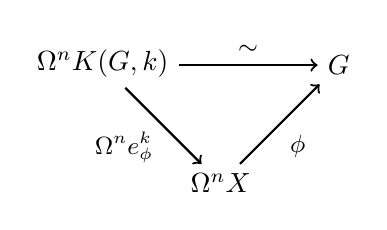
\begin{tikzpicture}[auto,node distance=2cm,
        thick,main node/.style={font=\sffamily\bfseries},text height=1.5ex]
      \node[main node] (OK) at (0,0) {$\Omega^nK(G,k)$};
      \node[main node] (G)  at (3,0) {$G$};
      \node[main node] (OX) at (1.5,-1.5) {$\Omega^n X$};
           \path[every node/.style={font=\sffamily\small}]
           (OK) edge [->] node {$\sim$} (G)
                edge [->] node [below left] {$\Omega^n e_\phi^k$} (OX)
           (OX) edge [->] node [below right] {$\phi$} (G);
    \end{tikzpicture}
  \end{center}
  Now if $\phi$ is a group isomorphism, by Whitehead's Theorem for truncated types \cite[Theorem 8.8.3]{TheBook} we know that $e_\phi^k$ is an equivalence, since it induces an equivalence on all homotopy groups (trivially on the levels other than $k$). We can also show that $e_\phi^k$ is natural in $\phi$.

  Note that if we have a group homomorphism $\psi:G\to G'$, we also get a group homomorphism $G\to\Omega^k K(G',k)$, and by the above construction we get a pointed map $K(\psi,k):K(G,k)\to_\pt K(G',k)$. This is functorial, which follows from naturality of $e_\phi^k$. 

  Finally, we can construct the equivalence explicitly. We have a functor
  $\pi_k:(0,k)\GType \to \AbGroup$ which sends $G$ to $\pi_k BG$. Conversely, we have the functor $K({-},k):\AbGroup\to (0,k)\GType$. We have natural isomorphisms
  $\pi_k K(G,k)\equiv G$ by~\autoref{thm:EM-spaces} and $K(\pi_k X,k)\equiv_\pt X$ by the application of Whitehead described above. The construction is exactly the same for $k=1$ after replacing $\AbGroup$ by $\Group$.
\end{proof}

\section{Stabilization}
\label{sec:stabilization}

In this section we discuss some constructions with higher groups~\cite{BaezDolan1998}. We will give the actions on the carriers and the deloopings, but we omit the third component, the pointed equivalence, for readability. We recommend keeping \autoref{tab:periodic} in mind during these constructions.
\begin{description}
\item[decategorification] $\Decat : (n,k)\GType \to (n-1,k)\GType$\\
  $\angled{G,B^kG} \mapsto \angled{\trunc{n-1}{G}, \trunc{n+k-1}{B^kG}}$
\item[discrete categorification] $\Disc : (n,k)\GType \to (n+1,k)\GType$ \\
  $\angled{G,B^kG} \mapsto \angled{G,B^kG}$
\end{description}
These functors make $(n,k)\GType$ a reflective sub-$(\infty,1)$-category of $(n+1,k)\GType$. That is, there is an adjunction ${\Decat} \dashv {\Disc}$. These properties are straightforward consequences of the universal property of truncation.

There are also iterated versions of these functors.
\begin{description}
  \item[$\infty$-decategorification] $\iDecat : (\infty,k)\GType \to (n,k)\GType$\\
    $\angled{G,B^kG} \mapsto \angled{\trunc{n}{G}, \trunc{n+k}{B^kG}}$
  \item[discrete $\infty$-categorification] $\iDisc : (n,k)\GType \to (\infty,k)\GType$ \\
    $\angled{G,B^kG} \mapsto \angled{G,B^kG}$
\end{description}
These functors satisfy the same properties: ${\iDecat} \dashv {\iDisc}$ such that the counit induces an isomorphism ${\iDecat} \circ {\iDisc} = \idfunc$.

For the next constructions, we need the following properties.
\begin{defn}
  For $A : \UU_\pt$ we define the \emph{$n$-connected cover} of $A$ to be 
  $A{\angled n} := \fib(A \to \trunc{n}{A})$. We have the projection $p_1: A{\angled n} \to_\pt A$.
\end{defn}
\begin{lem} \label{lem:connected-cover-univ}
  The universal property of the $n$-connected cover states the following. For any $n$-connected pointed type $B$, the pointed map
  $$(B \to_\pt A{\angled n}) \to_\pt (B \to_\pt A),$$
  given by postcomposition with $p_1$, is an equivalence.\\
\end{lem}
\begin{proof}
  Given a map $f:B\to_\pt A$, we can form a map $\widetilde f: B \to A{\angled n}$. First note that for $b:B$ the type $\tr{fb}_n=_{\trunc{n}{A}}\tr{\pt}_n$ is $(n-1)$-truncated and inhabited for $b=\pt$. Since $B$ is $n$-connected, the universal property for connected types shows that we can construct a $qb:\tr{fb}_n=\tr{\pt}_n$ for all $b$ such that $q_0:qb_0\cdot\mathsf{ap}_{\tr{\blank}_n}(f_0)=1$. Then we can define the map $\widetilde f(b):=(fb, qb)$. Now $\widetilde f$ is pointed, because $(f_0,q_0):(fb_0,qb_0)=(a_0,1)$.

  Now we show that this is indeed an inverse to the given map. On the one hand, we need to show that if $f: B \to_\pt A$, then $\proj 1 \circ \widetilde f=f$. The underlying functions are equal because they both send $b$ to $f(b)$. They respect points in the same way, because
  $\mathsf{ap}{p_1}(\widetilde f_0)=f_0$. The proof that the other composite is the identity follows from a computation using fibers and connectivity, which we omit here, but can be found in the formalization.
\end{proof}
The next reflective sub-$(\infty,1)$-category is formed by looping and delooping.
\begin{description}
\item[looping] $\Omega : (n,k)\GType \to (n-1,k+1)\GType$ \\
  $\angled{G,B^kG} \mapsto \angled{\Omega G,B^kG{\angled k}}$
\item[delooping] $\B : (n,k)\GType \to (n+1,k-1)\GType$ \\
  $\angled{G,B^kG} \mapsto \angled{\Omega^{k-1}B^kG,B^kG}$
\end{description}
We have ${\B} \dashv {\Omega}$, which follows from Lemma \ref{lem:connected-cover-univ} %note: autoref writes "Theorem"
and $\Omega\circ{\B} = \idfunc$, which follows from the fact that $A{\angled n}=A$ if $A$ is $n$-connected.

The last adjoint pair of functors is given by stabilization and forgetting. This does not form a reflective sub-$(\infty,1)$-category.
\begin{description}
\item[forgetting] $F : (n,k)\GType \to (n,k-1)\GType$ \\
  $\angled{G,B^kG} \mapsto \angled{G,\Omega B^kG}$
\item[stabilization] $S : (n,k)\GType \to (n,k+1)\GType$ \\
  $\angled{G,B^kG} \mapsto \angled{SG,\trunc{n+k+1}{\susp B^kG}}$,\\
  where $SG = \trunc{n}{\Omega^{k+1}\susp B^kG}$
\end{description}
We have the adjunction ${S} \dashv {F}$ which follows from the suspension-loop adjunction $\Sigma\dashv\Omega$ on pointed types.

The next main goal in this section is the stabilization theorem,
stating that the ditto marks in~\autoref{tab:periodic} are justified.

The following corollary is almost \cite[Lemma~8.6.2]{TheBook}, but
proving this in Book HoTT is a bit tricky. See the
formalization for details.
\begin{lem}[Wedge connectivity]
  \label{lem:wedge-connectivity}
  If $A : \UU_\pt$ is $n$-connected and $B: \UU_\pt$ is
  $m$-connected, then the map $A \vee B \to A \times B$ is
  $(n+m)$-connected.
\end{lem}

Let us mention that there is an alternative way to prove the wedge
connectivity lemma: Recall that if $A$ is $n$-connected and $B$ is
$m$-connected, then $A \ast B$ is
$(n+m+2)$-connected~\cite[Theorem~6.8]{joinconstruction}. Hence the
wedge connectivity lemma is also a direct consequence of the following lemma.
\begin{lem}
Let $A$ and $B$ be pointed types.
The fiber of the wedge inclusion $A\vee B\to A\times B$ is equivalent to
$\Omega{A}\ast\Omega{B}$. 
\end{lem}
\begin{proof}
Note that the fiber of $A\to A\times B$ is $\Omega B$, the fiber of $B\to A\times B$ is $\Omega A$, and of course the fiber of $1\to A\times B$ is $\Omega A\times \Omega B$. We get a commuting cube
\begin{equation*}
\begin{tikzcd}
& \Omega A\times \Omega B \arrow[dl] \arrow[d] \arrow[dr] \\
\Omega B \arrow[d] & 1 \arrow[dl] \arrow[dr] & \Omega A \arrow[dl,crossing over] \arrow[d] \\
A \arrow[dr] & 1 \arrow[d] \arrow[from=ul,crossing over] & B \arrow[dl] \\
& A\times B
\end{tikzcd}
\end{equation*}
in which the vertical squares are pullback squares. 

By the descent theorem for pushouts it now follows that $\Omega A\ast \Omega B$ is the fiber of the wedge inclusion.
\end{proof}

The second main tool we need for the stabilization theorem is:
\begin{thm}[Freudenthal]
  If $A : \UU_\pt^{>n}$ with $n\ge 0$, then the map
  $A \to \Omega\susp A$ is $2n$-connected.
\end{thm}
This is \cite[Theorem~8.6.4]{TheBook}.

The final building block we need is:
\begin{lem}
  There is a pullback square
  \[
    \begin{tikzcd}
      \susp\Omega A \ar[d,"\varepsilon_A"']\ar[r] & A \vee A \ar[d] \\
      A \ar[r,"\Delta"'] & A \times A
    \end{tikzcd}
  \]
  for any $A : \UU_\pt$.
\end{lem}

\begin{proof}
Note that the pullback of $\Delta:A\to A\times A$ along either inclusion $A\to A\times A$ is contractible. So we have a cube
\begin{equation*}
\begin{tikzcd}
& \Omega A \arrow[dl] \arrow[d] \arrow[dr] \\
1 \arrow[d] & 1 \arrow[dl] \arrow[dr] & 1 \arrow[dl,crossing over] \arrow[d] \\
A \arrow[dr] & A \arrow[d,"\Delta"] \arrow[from=ul,crossing over] & A \arrow[dl] \\
& A\times A
\end{tikzcd}
\end{equation*}
in which the vertical squares are all pullback squares. Therefore, if we pull back along the wedge inclusion, we obtain by the descent theorem for pushouts that the square in the statement is indeed a pullback square.
\end{proof}

\begin{thm}[Stabilization]
  \label{thm:stabilization}
  If $k\ge n+2$, then $S : (n,k)\GType \to (n,k+1)\GType$ is an
  equivalence, and any $G : (n,k)\GType$ is an infinite loop space.
\end{thm}
\begin{proof}
  We show that $F\circ S=\idfunc=S\circ F : (n,k)\GType \to (n,k)\GType$
  whenever $k\ge n+2$.

  For the first, the unit map of the adjunction factors as
  \[
    B^kG \to \Omega\susp B^kG \to \Omega\trunc{n+k+1}{\susp B^kG}
  \]
  where the first map is $2k-2$-connected by Freudenthal, and the
  second map is $n+k$-connected. Since the domain is $n+k$-truncated,
  the composite is an equivalence whenever $2k-2 \ge n+k$.

  For the second, the counit map of the adjunction factors as
  \[
    \trunc{n+k}{\susp\Omega B^kG} \to \trunc{n+k}{B^kG} \to B^kG,
  \]
  where the second map is an equivalence. By the two lemmas above, the
  first map is $2k-2$-connected.
\end{proof}
For example, for $G : (0,2)\GType$ an abelian group, we have
$B^nG = K(G,n)$, an Eilenberg-MacLane space.

The adjunction ${S} \dashv {F}$ implies that the free group on a
pointed set $X$ is $\Omega\trunc{1}{\susp X}=\pi_1(\susp X)$.  If $X$
has decidable equality, $\susp X$ is already $1$-truncated. It is an
open problem whether this is true in general.

Also, the abelianization of a set-level group $G : 1\mathsf{Grp}$ is
$\pi_2(\susp BG)$. If $G : (n,k)\GType$ is in the stable range ($k \ge
n+2$), then $SFG=G$.

\section{Perspectives on ordinary group theory}
\label{sec:perspectives}

In this section we shall indicate how the theory of higher groups can
yield a new perspective even on ordinary group theory.

From the symmetric groups $\Sym_n$, we can get other finite groups using
the constructions of~\autoref{sec:elementary-constructions}. Other
groups can be constructed more directly. For example,
$BA_n$, the classifying type of the alternating group, can be taken to
be the type of $n$-element sets $X$ equipped with a \emph{sign
  ordering}: this is an equivalence class of an ordering
$\Fin n \equiv X$ modulo even permutations. Indeed, there are only two
possible sign orderings, so this definition corresponds to
first considering the short exact sequence
\[
  1 \to A_n \to \Sym_n \xrightarrow{\mathrm{sgn}}{} \Sym_2 \to 1
\]
where the last map is the sign map, then realizing the sign map
as given by the map $\mathrm{Bsgn} : \BS_n \to \BS_2$ that takes
an $n$-element set to its set of sign orderings, and finally
letting $BA_n$ be the homotopy fiber of $\mathrm{Bsgn}$.

Similarly, $BC_n$, the classifying type of the cyclic group on $n$
elements, can be taken to be the type of $n$-elements sets $X$
equipped with a \emph{cyclic ordering}: an equivalence class of an
ordering $\Fin n \equiv X$ modulo cyclic permutations. But unlike
the above, where we had the coincidence that $\Aut(\Sym_2) \equiv
\Sym_2$,
this doesn't correspond to a short exact sequence. Rather,
it corresponds to a sequence
\[
  1 \to C_n \to \Sym_n \to \Aut(\Fin(n-1)) \equiv \Sym_{(n-1)!}
\]
where the delooping of the last map is the map from $\BS_n$ to
$\BS_{(n-1)!}$ that maps an $n$-element set to the set of cyclic
orderings, of which there are $(n-1)!$ many -- since once we fix the
position in the ordering of a particular element,
we are free to permute the rest.

As another example,
consider the map $p : \BS_4 \to_\pt \BS_3$ that maps a 4-element set
$X$ to its set of 2-by-2 partitions, of which there $3$. Using this
construction, we can realize some famous semidirect and wreath product identities,
such as $A_4 \equiv S_2^2 \rtimes A_3$, $S_4 \equiv S_2^2 \rtimes
S_3$, and, for the octahedral group, $O_h \equiv S_2^3 \rtimes S_3
\equiv S_2 \wr S_3$.

\smallskip

Let us turn to a different way of getting new groups from old, namely
via covering space theory.

\subsection{\texorpdfstring{$1$}{1}-groups and covering spaces}
\label{sec:covering}

The connection between covering spaces of a pointed connected type
$X$ and sets with an action of the fundamental group of $X$ has
already been established in homotopy type
theory~\cite{FavoniaHarper2016}. Let us recall this connection and
expand a bit upon it.

For us, a pointed connected type $X$ is equivalently
an $\infty$-group $G:\infty\mathsf{Grp}$
with delooping $BG := X$.
A covering space over $BG$ is simply a type family $C : BG \to \mathsf{Set}$
that lands in the universe of sets.
Hence by our discussion of actions in~\autoref{sec:actions}
it is precisely a set with a $G$-action.
Since $\mathsf{Set}$ is a 1-type, $C$ extends uniquely to a type family
$C' : \trunc{1}{BG} \to \mathsf{Set}$,
but $\trunc{1}{BG}$ is the delooping of the fundamental group
of $X$, and hence $C'$ is the uniquely determined
choice of a set with an action of the fundamental group.

The universal covering space is the simply connected cover of $BG$,
\[
  \widetilde{BG} : BG \to \mathsf{Set}, \quad
  z \mapsto \trunc{0}{\pt = z}.
\]
Note that the total space of $\widetilde{BG}$ is indeed the
$1$-connected cover $BG\angled1$,
since $\trunc{0}{\pt =_{BG} \pt} \equiv (\tr{\pt} =_{\trunc{1}{BG}} \tr{\pt})$.
Also note that if $G$ is already a 1-group, then this is just the right
action of $G$ on itself, and in general, it is the right action of $G$
on the fundamental group
(i.e., the decategorification of $G$)
via the truncation homomorphism from $G$ to $\pi_1(BG)$,
where we can also view $\pi_1(BG)$ as the $1\mathsf{Grp}$ decategorification
of $G$.

In general, there is a Galois correspondence between connected covers
of $BG$ and conjugacy classes of subgroups of the fundamental group.
Indeed, if $C : BG \to \mathsf{Set}$ has a connected total space,
then the space $(g : \trunc{1}{BG}) \times C'(g)$
is itself a connected, 1-truncated type,
and the projection to $\trunc{1}{BG}$
induced an inclusion of fundamental groups
once a point $\pt : C'(\pt)$ has been chosen.

\begin{thm}[Fundamental theorem of Galois theory for covering spaces]
  \label{thm:galois-zero}
  $\phantom{42}$
  \begin{enumerate}
  \item  The automorphism group of the universal covering space
    $\widetilde{BG}$ is isomorphic to
    the $1$-group decategorification of $G$,
    \[
      \Aut(\widetilde{BG}) \equiv \Decat_1(G) \equiv \pi_1(BG).
    \]
  \item Furthermore, there is a contravariant correspondence between
    conjugacy classes of subgroups of $\Decat_1(G)$ and connected
    covers of $BG$.
  \item This lifts to a Galois correspondence between subgroups of
    $\Decat_1(G)$ and pointed, connected covers of $BG$.  The normal
    subgroups correspond to Galois covers.
  \end{enumerate}
\end{thm}
Note that the universal covering space
and the trivial covering space
(constant at the unit type)
are canonically pointed,
reflecting the fact that
the two trivial subgroups are normal.

The first part of the fundamental theorem has a clear generalization to
higher groups:
\begin{thm}[Fundamental theorem of Galois theory for $n$-covers,
  part one]
  The automorphism group of the universal $n$-type cover $U_n(BG)$,
  \[
    U_n(BG) : BG \to \UU^{\le n},
    \quad
    z \mapsto \trunc{n}{\pt = z}
  \]
  of $BG$ is
  isomorphic to the $(n+1)$-group decategorification of $G$,
  \[
    \Aut(U_n(BG)) \equiv \Decat_{n+1}(G) \equiv \Pi_{n+1}(BG).
  \]
\end{thm}
\begin{proof}
  Note that
  $\BAut(U_n(BG))$ is the image of the map $1 \to (BG \to \UU^{\le
    n})$ that sends the canonical element to $U_n(BG)$. Since $BG$ is
  connected, this image is exactly $\trunc{n+1}{BG}$ by
  \cite[Theorem~7.1]{joinconstruction}. Then we are done,
  since $\B\Pi_{n+1}(BG) \equiv \trunc{n+1}{BG}$, by definition.
\end{proof}
It is possible to use the other parts
of~\autoref{thm:galois-zero} in order to \emph{define} the notions of
subgroup and normal subgroup for $n$-groups, which then become
\emph{structure on} rather than a \emph{property of} a homomorphism $f
: K \to G$.
Explicitly, the structure of a \emph{normal subgroup} on such an $f$
is a delooping $B(G \dblslash K)$ of the type $G \dblslash K$
together with a map $Bq : BG \to_\pt B(G \dblslash K)$ giving rise to a
fiber sequence
\begin{equation}\label{eq:normal-fiber-sequence}
  G \dblslash K \to BK \xrightarrow{Bf}{} BG
  \xrightarrow{Bq}{} B(G \dblslash K).
\end{equation}

\subsection{Central extensions and group cohomology}
\label{sec:group-cohomology}

The cohomology of a higher group $G$ is simply the cohomology of its
delooping $BG$. Indeed, for any spectrum $A$, we define
\[
  H_{\mathrm{Grp}}^k(G, A) := \trunc{0}{BG \to_\pt B^kA}.
\]
Of course, to define the $k$'th cohomology group, we only need the
$k$-fold delooping $B^kA$.

If $A:(\infty,2)\GType$ is a braided $\infty$-group, then
we have the second cohomology group $H_{\mathrm{Grp}}^2(G, A)$, and an
element $c:BG \to_\pt B^2A$ gives rise to a \emph{central extension}
\[
  BA \to BH \to BG \xrightarrow{c}{} B^2A,
\]
where $BH$ is the homotopy fiber of $c$.  This lifts to the world of
higher groups the usual result that isomorphism classes of central
extensions of a $1$-group $G$ by an abelian $1$-group $A$
are given by cohomology classes in $H_{\mathrm{Grp}}^2(G, A)$.

\smallskip

In the Spectral repository there is full formalization of the Serre
spectral sequence for cohomology \cite{SerreSpectralSequence}.
If we have any normal subgroup fiber sequence for $\infty$-groups as
in~\eqref{eq:normal-fiber-sequence}, then we get a corresponding
spectral sequence with $E_2$-page
\[
  H_{\mathrm{Grp}}^p(G \dblslash K, H_{\mathrm{Grp}}^q(K, A))
\]
and converging to $H_{\mathrm{Grp}}^n(G, A)$, where $A$ is any
truncated, connective spectrum, which could even be a left $G$-module,
in which case we reproduce the \emph{Hochschild-Serre spectral
  sequence}.


\chapter{Projective spaces}

\section{The real projective spaces}
In this section I describe joint work with Ulrik Buchholtz \cite{realprojective}, in which we defined the real projective spaces $\rprojective{n}$ in homotopy type theory. Furthermore, I answer a question posed by André Joyal during his visit of CMU in February 2018, regarding the complement of the tautological bundle on $\rprojective{n}$.

\subsection{The type of $2$-element sets}

\begin{lem}\label{lem:isequiv_evunit}
The map
\begin{equation*}
\evunit : (\eqv{\sphere{0}}{\sphere{0}})\to \sphere{0}.
\end{equation*}
given by $e\mapsto e(\north)$ is an equivalence. 
\end{lem}

\begin{proof}
The map in the converse direction is definec by case analysis:
\begin{align*}
\north & \mapsto \idfunc \\
\south & \mapsto \bneg.
\end{align*}
It is straightforward to verify that this defines the inverse of $\evunit$.
\end{proof}

\begin{thm}\label{thm:ptd_2elt_sets}
The type
\begin{equation*}
\sm{A:\UU_{\sphere{0}}}A
\end{equation*}
of pointed $2$\nobreakdash-element sets is contractible.
\end{thm}

\begin{proof}
We take $\pairr{\sphere{0},\north}$ as the center of contraction.
To define the contraction, we will show that the identity type $\pairr{\sphere{0},\north}=\pairr{A,a}$ is contractible, for any $A:\UU_{\sphere{0}}$ and $a:A$. This might look stronger than necessary, but since being contractible is a proposition we get to assume that $\id{\sphere{0}}{A}$ by induction on $\brck{\sphere{0}=A}$. Then we proceed by path induction, so it suffices to show that the type
\begin{equation*}
\pairr{\sphere{0},\north}=\pairr{\sphere{0},a}
\end{equation*}
is contractible, for any $a:\sphere{0}$. We note that there is an equivalence
\begin{equation*}
\eqv{\Big(\pairr{\sphere{0},\north}=\pairr{\sphere{0},a}\Big)}{\Big(\sm{e:\eqv{\sphere{0}}{\sphere{0}}}e(\north)=a\Big)}.
\end{equation*}
by \autoref{lem:equiv_of_ptdtype}, and the latter type is just the fiber of $\mathsf{ev\usc{}unit}$. Thus the claim follows by \cref{lem:isequiv_evunit}.
\end{proof}

\begin{cor}\label{cor:id_U2}
The canonical map
\begin{equation*}
\mathsf{pt\usc{}eq} : \prd{A:\UU_{\sphere{0}}} ({\sphere{0}}= A)\to A
\end{equation*}
given by $\mathsf{pt\usc{}eq}(\refl{\sphere{0}})\defeq \north$ is an equivalence. We will write
\begin{equation*}
\mathsf{eq\usc{}pt} : \prd{A:\UU_{\sphere{0}}} A \to (\sphere{0}=A)
\end{equation*}
for the inverse fiberwise transformation.
\end{cor}

\begin{proof}
Immediate by \cref{thm:id_fundamental}.
\end{proof}

Another way of stating the following theorem, is by saying that the map
$\unit\to\UU_{\sphere{0}}$ classifies the ${\sphere{0}}$\nobreakdash-bundles.

\begin{cor}\label{lem:classifyer_U2}
Let $B:A\to\UU_{\sphere{0}}$ be a ${\sphere{0}}$\nobreakdash-bundle. Then the square
\begin{equation*}
\begin{tikzcd}
\sm{x:A}B(x) \arrow[r] \arrow[d,swap,"\proj 1"] & \unit \arrow[d,"{\sphere{0}}"] \\
A \arrow[r,swap,"B"] & \UU_{\sphere{0}},
\end{tikzcd}
\end{equation*}
which commutes via the homotopy $\lam{(x,y)}\mathsf{eq\usc{}pt}(y)^{-1}$, is a pullback square. 
\end{cor}

\subsection{Finite dimensional real projective spaces}
\label{sec:fdrp}

Classically, the $(n+1)$-st real projective space can be obtained by attaching an $(n+1)$-cell to the $n$-th real projective space. This suggests a way of defining the real projective spaces that involves simultaneously defining $\rprojective{n}$ and an attaching map $\alpha_n : \sphere{n}\to\rprojective{n}$. Then we obtain $\rprojective{n+1}$ as the mapping cone of $\alpha_n$, i.e., as a pushout
\begin{equation*}
\begin{tikzcd}
\sphere{n} \arrow[r,"\alpha_n"] \arrow[d] & \rprojective{n} \arrow[d] \\
\unit \arrow[r] & \rprojective{n+1},
\end{tikzcd}
\end{equation*}
and we have to somehow find a way to define the attaching map $\alpha_{n+1}:\sphere{n+1}\to\rprojective{n}$ to continue the inductive procedure.
However, it is somewhat tricky to obtain these attaching maps directly, and we have chosen to follow a closely related path towards the definition of the real projective spaces that takes advantage of the machinery of dependent type theory. 

Observe that the attaching map $\alpha_n:\sphere{n}\to\rprojective{n}$ is just the tautological bundle (or the quotient map that identifies the antipodal points). This suggests that we may proceed by defining simultaneously the real projective space $\rprojective{n}$ and its tautological bundle $\tautfam[\R]{n}$. The tautological bundle on $\rprojective{n}$ is an $\sphere{0}$-bundle, so it can be described as a map $\rprojective{n}\to\UU_{\sphere{0}}$. We perform this construction in \autoref{defn:realprojective} using the properties of the type of 2-element types developed in \autoref{sec:UUS0}, and in \autoref{thm:Sn_totalcov} we show that the total space of the tautological bundle on $\rprojective{n}$ is the $n$-sphere. 

\begin{defn}\label{defn:realprojective}
We define simultaneously for each $n:\N_{-1}$, 
the \define{$n$-dimensional real projective space} $\rprojective{n}$, 
and the \define{tautological bundle} $\tautfam[\R]{n}:\rprojective{n}\to \UU_{\sphere{0}}$.
\end{defn}

\begin{proof}[Construction]
The construction is by induction on $n:\N_{-1}$.
For the base case $n\defeq -1$, 
we take $\rprojective{-1}\defeq\emptyt$. 
Then there is a unique map of type $\rprojective{-1}\to \UU_{\sphere{0}}$, which we
take as our definition of $\tautfam[\R]{-1}$.

For the inductive step, suppose $\rprojective{n}$ and $\tautfam[\R]{n}$ are defined. Then we define $\rprojective{n+1}$ to be the pushout
\begin{equation*}
\begin{tikzcd}
{\sm{x:\rprojective{n}}\tautfam[\R]{n}(x)} \arrow[d,swap,"\proj 1"] \arrow[r] & \unit \arrow[d,"\base"] \\
\rprojective{n} \arrow[r,swap,"\inr"] & \rprojective{n+1}
\end{tikzcd}
\end{equation*}
In other words, 
$\rprojective{n+1}$ is the \emph{mapping cone} of the tautological bundle, 
when we view the tautological bundle as the projection 
$\proj 1:(\sm{x:\rprojective{n}}\tautfam[\R]{n}(x))\to\rprojective{n}$. 

To define $\tautfam[\R]{n+1}:\rprojective{n+1}\to \UU_{\sphere{0}}$
we use the universal property of $\rprojective{n+1}$. 
Therefore, it suffices to show that the outer square in the diagram
\begin{equation}\label{eq:diagram}
\begin{tikzcd}
{\sm{x:\rprojective{n}}\tautfam[\R]{n}(x)} \arrow[d,swap,"\proj 1"] \arrow[r] & \unit \arrow[d,swap,"\base"] \arrow[ddr,bend left=15,"\sphere{0}"]\\
\rprojective{n} \arrow[drr,bend right=15,swap,"{\tautfam[\R]{n}}"] \arrow[r,swap,"\inr"] & \rprojective{n+1} \arrow[dr,densely dotted] \\
& & \UU_{\sphere{0}}
\end{tikzcd}
\end{equation}
commutes. Indeed, in \autoref{lem:classifyer_U2} we have constructed a homotopy 
\begin{equation*}
R_n\defeq R_{\rprojective{n},\tautfam[\R]{n}}:\prd{x:\rprojective{n}}{y:\tautfam[\R]{n}} \eqv{\tautfam[\R]{n}(x)}{\sphere{0}},
\end{equation*}
and in fact, this square is a pullback.
\end{proof}

\begin{eg}
We have $\rprojective{-1}=\emptyt$, $\rprojective{0}=\unit$, and $\rprojective{1}=\sphere{1}$. 
\end{eg}

\begin{thm}\label{thm:Sn_totalcov}
For each $n:\N_{-1}$, there is an equivalence
\begin{equation*}
e_n:\eqv{\sphere{n}}{\sm{x:\rprojective{n}}\tautfam[\R]{n}(x)}.
\end{equation*}
\end{thm}

In other words, $\rprojective{n+1}$ is obtained from $\rprojective{n}$ by attaching a single $(n+1)$\nobreakdash-disk, i.e., as a pushout
\begin{equation*}
\begin{tikzcd}
\sphere{n} \arrow[r] \arrow[d,swap,"\proj1\circ e_n"] & \unit \arrow[d] \\
\rprojective{n} \arrow[r] & \rprojective{n+1}.
\end{tikzcd}
\end{equation*}

\begin{proof}
For $n\jdeq -1$, we have $\rprojective{-1}\jdeq\emptyt$ and the unique tautological bundle $\tautfam[\R]{-1}$. Therefore the type $\sm{x:\rprojective{-1}}\tautfam[\R]{-1}(x)$ is equivalent to the empty type, which is $\sphere{-1}$ by definition. This gives the base case.

Now assume that we have an equivalence $e_n:\eqv{\sphere{n}}{\sm{x:\rprojective{n}}\tautfam[\R]{n}(x)}$. 
Our goal is to construct the equivalence
\begin{equation*}
e_{n+1}:\eqv{\sphere{n+1}}{\sm{x:\rprojective{n+1}}\tautfam[\R]{n+1}(x)}.
\end{equation*}
such that the square
\begin{equation}\label{eq:Sn_totalcov_natural}
\begin{tikzcd}
\sphere{n} \arrow[d,swap,"e_{n}"] \arrow[r,"\inl"] & \sphere{n+1} \arrow[d,"e_{n+1}"] \\
\sm{x:\rprojective{n}}\tautfam[\R]{n}(x) \arrow[r] & \sm{x:\rprojective{n+1}}\tautfam[\R]{n+1}(x)
\end{tikzcd}
\end{equation}
commutes. By the functoriality of the join (or equivalently, by equivalence induction on $e_n$), it suffices to find an equivalence
\begin{equation*}
\alpha:\eqv{\join{\Big(\sm{x:\rprojective{n}}\tautfam[\R]{n}(x)\Big)}{\sphere{0}}}{\sm{x:\rprojective{n+1}}\tautfam[\R]{n+1}(x)},
\end{equation*}
such that the bottom triangle in the diagram
\begin{equation*}
\begin{tikzcd}
\sphere{n} \arrow[r,"\inl"] \arrow[d,swap,"e_n"] & \sphere{n+1} \arrow[d,"\join{e_n}{\idfunc[\sphere{0}]}"] \\
\sm{x:\rprojective{n}}\tautfam[\R]{n}(x) \arrow[r,"\inl"] \arrow[dr] & \join{\Big(\sm{x:\rprojective{n}}\tautfam[\R]{n}(x)\Big)}{\sphere{0}} \arrow[d,"\alpha"] \\
& \sm{x:\rprojective{n+1}}\tautfam[\R]{n+1}(x)
\end{tikzcd}
\end{equation*}
commutes.
We construct this equivalence using the flattening lemma, \autoref{lem:flattening}, from which we get a pushout square:
\begin{equation*}
\begin{tikzcd}[column sep=0.5em]
\sm{x:\rprojective{n}}{y:\tautfam[\R]{n}(x)}\tautfam[\R]{n}(x) \arrow[r] \arrow[d] & \sm{t:\unit}\sphere{0} \arrow[d] \\
\sm{x:\rprojective{n}}\tautfam[\R]{n}(x) \arrow[r] & \sm{x:\rprojective{n+1}}\tautfam[\R]{n+1}(x)
\end{tikzcd}
\end{equation*}
We can calculate this pushout by constructing a natural transformation of spans (diagrams in $\UU$ of the form $\cdot\leftarrow\cdot\rightarrow\cdot$), as indicated by the diagram in Fig.~\ref{fig:sphere-equiv}.
\begin{figure*}
  \centering
\begin{tikzcd}[column sep=6em]
\sm{x:\rprojective{n}}\tautfam[\R]{n}(x) \arrow[d,swap,"\idfunc"]
  & \sm{x:\rprojective{n}}{y:\tautfam[\R]{n}(x)}\tautfam[\R]{n}(x) \arrow[l,swap,"\pairr{x,z}\mapsfrom\pairr{x,y,z}" yshift=1ex] \arrow[d,densely dotted,"u"] \arrow[r,"\pairr{x,y,z}\mapsto\pairr{\ttt,R_n(x,y,z)}" yshift=1ex] 
  & \sm{t:\unit}\sphere{0} \arrow[d,"\proj 2"] \\
\sm{x:\rprojective{n}}\tautfam[\R]{n}(x)
  &
\Big(\sm{x:\rprojective{n}}\tautfam[\R]{n}(x)\Big)\times\sphere{0} \arrow[l,"\pi_1"] \arrow[r,swap,"\pi_2"]
  & \sphere{0}
\end{tikzcd}
\caption{Map of spans used in the proof of Thm~\ref{thm:Sn_totalcov}. The map $u$ is given by $\pairr{x,y,z}\mapsto\pairr{x,z,R_n(x,y,z)}$.}
\label{fig:sphere-equiv}
\end{figure*}
To show that the map $u$ in Fig.~\ref{fig:sphere-equiv} is an equivalence, it suffices to show that $R_n(x,y,z)=R_n(x,y,z)$ for any $x$, $y$, and $z$, because then it follows that $u$ is homotopic to the total map of a fiberwise equivalence. More generally, it suffices to show that $R_{\UU_{\sphere{0}},T}(X,x,y)=R_{\UU_{\sphere{0}},T}(X,y,x)$, where $T$ is the tautological bundle on $\UU_{\sphere{0}}$. Since $\UU_{\sphere{0}}$ is connected and since our goal is a mere proposition, we only need to verify the claim at the base point $\sphere{0}$ of $\UU_{\sphere{0}}$. This boils down to verifying that the group multiplication of $\Zmodtwo$ is indeed commutative.
\end{proof}

\begin{cor}
We obtain the fiber sequence
\begin{equation*}
\begin{tikzcd}
\sphere{0} \arrow[r,hook] & \sphere{n} \arrow[r,->>] & \rprojective{n}.
\end{tikzcd}
\end{equation*}
Hence, for each $k\geq 2$ we have $\pi_k(\sphere{n})=\pi_k(\rprojective{n})$. 
\end{cor}

\begin{proof}
Since we have the double cover $\tautfam[\R]{n}:\rprojective{n}\to\UU_{\sphere{0}}$ with total space $\sphere{n}$, we obtain the long exact sequence
\begin{equation*}
\begin{tikzcd}
  \cdots \arrow[r]
  & \pi_{k+1}(\sphere{n}) \arrow[r] \arrow[d, phantom, ""{coordinate, name=Z}]
  & \pi_{k+1}(\rprojective n) \arrow[dll, rounded corners,
      to path={ -- ([xshift=8.5ex]\tikztostart.center)
                |- (Z) [near end]\tikztonodes
                -| ([xshift=-8ex]\tikztotarget.center) -- (\tikztotarget)}] \\
  \pi_k(\sphere{0}) \arrow[r]
  & \pi_k(\sphere{n}) \arrow[r] \arrow[d, phantom, ""{coordinate, name=W}]
  & \pi_k(\rprojective n) \arrow[dll, rounded corners,
      to path={ -- ([xshift=8.5ex]\tikztostart.center)
                |- (W) [near end]\tikztonodes
                -| ([xshift=-8ex]\tikztotarget.center) -- (\tikztotarget)}] \\
  \pi_{k-1}(\sphere{0}) \arrow[r]
  & \pi_{k-1}(\sphere{n}) \arrow[r]
  & \cdots
\end{tikzcd}
\end{equation*}
Since $\pi_k({\sphere{0}})=0$ for $k\geq 1$, we get the desired isomorphisms.
\end{proof}

\subsection{The infinite dimensional real projective space}
\label{sec:idrp}

Observe that from the definition of $\rprojective{n}$ and its tautological 
cover, we obtain a commutative diagram of the form:
\begin{equation*}
\begin{tikzcd}[row sep=large,column sep=large]
\rprojective{-1} \arrow[r,"\inr"] \arrow[dr,swap,"{\tautfam[\R]{-1}}"] 
& \rprojective{0} \arrow[d,swap,near start,"{\tautfam[\R]{0}}"] \arrow[r,"\inr"] 
& \rprojective{1} \arrow[dl,swap,"{\tautfam[\R]{1}}"] \arrow[r,"\inr"] 
& \cdots \arrow[dll,"{\tautfam[\R]{2}}"]\\
& \UU_{\sphere{0}}
\end{tikzcd}
\end{equation*}
Using this sequence, we define the infinite dimensional real projective space
and its tautological cover:

\begin{defn}
We define the \define{infinite real projective space} $\rprojective{\infty}$ to be the sequential colimit of the finite real projective spaces. The double covers on $\rprojective{n}$ define a cocone on the type sequence of real projective spaces, so we also obtain $\tautfam[\R]{\infty}:\rprojective{\infty}\to \UU_{\sphere{0}}$. 
\end{defn}

\begin{thm}\label{thm:RPoo_US0}
The double cover $\tautfam[\R]{\infty}$ is an equivalence from $\rprojective{\infty}$ to $\UU_{\sphere{0}}$. 
\end{thm}

\begin{proof}
We have to show that the fibers of $\tautfam[\R]{\infty}$ are contractible.
Since being contractible is a mere proposition, and since the type $\UU_{\sphere{0}}$
is connected, it suffices to show that the fiber
\begin{equation*}
\sm{x:\rprojective{\infty}}\sphere{0}=\tautfam[\R]{\infty}(x)
\end{equation*}
of $\tautfam[\R]{\infty}$ at $\sphere{0}:\UU_{\sphere{0}}$ is contractible.
By \autoref{cor:id_U2} we have an equivalence of type
\begin{equation*}
\eqv{({\sphere{0}}=\tautfam[\R]{\infty}(x))}{\tautfam[\R]{\infty}(x)},
\end{equation*}
for every $x:\rprojective{\infty}$. 
Therefore it is equivalent to show that the type
\begin{equation*}
\sm{x:\rprojective{\infty}}\tautfam[\R]{\infty}(x)
\end{equation*}
is contractible. The general version of the flattening lemma, as stated in
Lemma 6.12.2 in \cite{hottbook}, can be adapted for sequential colimits, so
we can pull the colimit out: it suffices to prove that
\begin{equation*}
\tfcolim_n\bigl(\sm{x:\rprojective{n}}\tautfam[\R]{n}(x)\bigr)
\end{equation*}
is contractible. 
To do this, observe that the equivalences of \autoref{thm:Sn_totalcov} form
a natural equivalence of type sequences as shown in Fig.~\ref{fig:type-sequences}.
\begin{figure*}
  \centering
\begin{tikzcd}
\sm{x:\rprojective{-1}}\tautfam[\R]{-1}(x) \arrow[r] \arrow[d,swap,"\eqvsym"]
& \sm{x:\rprojective{0}}\tautfam[\R]{0}(x) \arrow[r] \arrow[d,swap,"\eqvsym"]
& \sm{x:\rprojective{1}}\tautfam[\R]{1}(x) \arrow[r] \arrow[d,swap,"\eqvsym"]
& \cdots \\
\sphere{-1} \arrow[r] 
& \sphere{0} \arrow[r]
& \sphere{1} \arrow[r]
& \cdots
\end{tikzcd}
\caption{Natural equivalence of type sequences for Thm~\ref{thm:RPoo_US0}.}
\label{fig:type-sequences}
\end{figure*}
Indeed, the naturality follows from \autoref{eq:Sn_totalcov_natural}.

Thus, the argument comes down to showing that $\sphere{\infty}\defeq\tfcolim_n(\sphere{n})$
is contractible. This was first shown in homotopy type theory by Brunerie, and
the argument is basically that the sequential colimit of a type sequence of
strongly constant maps (viz., maps factoring through $\unit$) is always contractible.
\end{proof}

\begin{rmk}
Note that by our assumption that the universe is closed under pushouts, it
follows that each $\rprojective{n}$ is in $\UU$. 
Since the universe contains a natural numbers object $\N$, 
it also follows that the universe is closed under sequential colimits,
and therefore we have $\rprojective{\infty}:\UU$. 
Whereas a priori it is not clear that $\UU_{\sphere{0}}$ is equivalent to a 
$\UU$-small type, this fact is contained in \autoref{thm:RPoo_US0}.
\end{rmk}

\subsection{The real projective spaces as classifying spaces}
In this subsection I answer a question posed by André Joyal during his visit of CMU in February 2018, regarding the complement of the tautological bundle on $\rprojective{n}$. The question was to construct in homotopy type theory an $\sphere{n}$-bundle $\beta^n$ over $\rprojective{n+1}$, equipped with equivalences $\eqv{\sphere{n+1}}{\join{\beta^n(x)}{\gamma^n(x)}}$ for every $x:\rprojective{n+1}$, and moreover that $\rprojective{n+1}$ classifies types $X$ with an $\sphere{0}$-bundle and an $\sphere{n}$-bundle that become trivial when joined together. 

\begin{defn}
We construct for $n\geq 0$ an $\sphere{n-1}$-bundle $\orthcomp[\R]{n}$ on $\rprojective{n}$ such that
\begin{equation*}
\eqv{\join{\orthcomp[\R]{n}(x)}{\tautfam[\R]{n}(x)}}{\sphere{n}}.
\end{equation*}
\end{defn}

\begin{proof}[Construction]
We will construct for any $n\geq 0$ a term of type
\begin{equation*}
\prd{x:\rprojective{n}} \sm{X:\BAut(\sphere{n-1})} \eqv{\join{X}{\tautfam[\R]{n}(x)}}{\sphere{n}}.
\end{equation*}
For the base case we have to define a term of type
\begin{equation*}
\prd{x:\rprojective{0}} \sm{X:\BAut(\sphere{-1})} \eqv{\join{X}{\sphere{0}}}{\sphere{0}}.
\end{equation*}
We simply choose $X\jdeq \emptyt$, and the canonical equivalence $\eqv{\join{\emptyt}{\sphere{0}}}{\sphere{0}}$. 

For the inductive step suppose we have for every $x:\rprojective{n}$ a type $\orthcomp[\R]{n}(x)$ and an equivalence
\begin{equation*}
\eqv{\join{C(x)}{\tautfam[\R]{n}(x)}}{\sphere{n}}.
\end{equation*}
Our goal is to construct for every $x:\rprojective{n+1}$ a type $\orthcomp[\mathbb{R}]{n+1}(x)$ equipped with an equivalence
\begin{equation*}
\eqv{\join{\orthcomp[\mathbb{R}]{n+1}(x)}{\tautfam[\R]{n+1}(x)}}{\sphere{n+1}}.
\end{equation*}
We do this by the universal property of $\rprojective{n+1}$. Thus, it suffices to construct
\begin{align*}
B_{\pt} & : \sm{X:\BAut(\sphere{n})}\eqv{\join{X}{\sphere{0}}}{\sphere{n}}.\\
B_i & : \prd{x:\rprojective{n}}\sm{X:\BAut(\sphere{n})}\eqv{\join{X}{\tautfam[\R]{n}(x)}}{\sphere{n}} \\
B_p & : \prd{x:\rprojective{n}}{y:\tautfam[\R]{n}(x)} ... 
\end{align*}
\end{proof}

\begin{lem}
For any two $2$-element sets $T$ and $T'$ with $t:T$ and $t':T'$, the square
\begin{equation*}
\begin{tikzcd}
\join{T}{T'} \arrow[r] \arrow[d] & \join{T'}{T} \arrow[d] \\
\join{T}{T'} \arrow[r] & \join{\bool}{\bool}
\end{tikzcd}
\end{equation*}
commutes.
\end{lem}

\begin{proof}
Since $\eqv{T}{(T=\bool)}$ it suffices to show that
\begin{equation*}
\join{\mathsf{neg}}{\idfunc}\htpy \sigma.
\end{equation*}
This is straightforward to verify by the universal property of $\join{\bool}{\bool}$. 
\end{proof}
\section{The complex projective spaces}

\section{The quaternionic Hopf fibration}
\section{The classical Cayley-Dickson construction}
\label{sec:cayley-dickson}

Classically, the $1$-, $3$- and $7$-dimensional spheres are subspaces of
$\mathbb{R}^2$, $\mathbb{R}^4$ and $\mathbb{R}^8$, respectively. Each
of these vector spaces can be given the structure of a normed division
algebra, and we get the complex numbers $\mathbb{C}$, Hamilton's
quaternions $\mathbb{H}$, and the octonions $\mathbb{O}$ of Graves and
Cayley. Since, in each of these algebras, the product preserves norm,
the unit sphere is a subgroup of the multiplicative group.

Cayley's construction of the octonions was later generalized by
Dickson \cite{Dickson1919}, who gave a uniform procedure for
generating each of these algebras from the previous one. The process
can be continued indefinitely, giving for instance the $16$-dimensional
sedenion-algebra after the octonions.

Here we describe one variant of the Cayley-Dickson construction,
following the presentation in \cite{Baez2002}. For this purpose, let
an \emph{algebra} be a vector space $A$ over $\mathbb R$ together with
a bilinear multiplication, which need not be associative, and a unit
element $1$. A \emph{$*$-algebra} is an algebra equipped with a linear involution
$*$ (called the \emph{conjugation}) satisfying $1^*=1$ and $(ab)^*=b^*a^*$.

If $A$ is a $*$-algebra, then $A' \defeq A\oplus A$ is again a
$*$-algebra using the definitions
\begin{equation}
  \label{eq:classical-cd}
  (a,b)(c,d) := (ac - db^*, a^*d + cb),
  \quad 1 := (1,0),
  \quad (a,b)^* := (a^*,-b).
\end{equation}
If $A$ is \emph{nicely normed} in the sense that (i) for all $a$, we have $a+a^*\in \mathbb R$
(i.e., the subspace spanned by $1$), and (ii) $aa^*=a^*a>0$ for
nonzero $a$, then so is $A'$. In the nicely normed case, we get a norm by defining
\[\norm a = aa^*,\]
and we have inverses given by $a^{-1}=a^*/\norm a$.
By applying this construction repeatedly, starting with $\mathbb{R}$, we obtain the
following sequence of algebras, each one having slightly fewer good
properties than the preceding one:
\begin{itemize}
\item $\mathbb R$ is a \emph{real} (i.e., $a^*=a$) commutative associative
  nicely normed $*$-algebra,
\item $\mathbb C$ is a commutative associative nicely normed $*$-algebra,
\item $\mathbb H$ is an associative nicely normed $*$-algebra,
\item $\mathbb O$ is an \emph{alternative} (i.e., any subalgebra generated by
  two elements is associative) nicely normed $*$-algebra,
\item the sedenions and the following algebras are nicely normed
  $*$-algebras, which are neither commutative, nor alternative.
\end{itemize}
Being alternative, the first four are normed division algebras, as
$a,b,a^*,b^*$ are in the subalgebra generated by $a-a^*$ and $b-b^*$,
so we get
\[ \norm{ab}^2 = (ab)(ab)^* = (ab)(b^*a^*) = a(bb^*)a^* = \norm
  a^2\norm b^2.\]
However, starting with the sedenions, this fails and we get nontrivial
zero divisors. In fact, the zero divisors of norm one in the sedenions
form a group homeomorphic to the exceptional Lie group $G_2$.

To sum up the story as it relates to us, we first form the four normed
division algebras $\mathbb R$, $\mathbb C$, $\mathbb H$ and $\mathbb
O$ by applying the Cayley-Dickson construction starting with $\mathbb
R$, and then we carve out the unit spheres and get spaces with
multiplication $\Sn^0$, $\Sn^1$, $\Sn^3$ and $\Sn^7$.

In homotopy type theory, we cannot use this strategy directly. Before we
discuss our alternative construction, let us recall some basics
regarding H-spaces in homotopy type theory.

\section{Spheroids and imaginaroids}
\label{sec:imaginaroids}

We saw in Section~\ref{sec:cayley-dickson} the classical
Cayley-Dickson construction on the level of $*$-algebras. We would obtain nothing
of interest by imitating this directly in homotopy type theory, as any real vector
space is contractible and thus equivalent to the one-point type $1$.

A first idea, which turns out to not quite work, is to give an
analog of the Cayley-Dickson construction on the level of the unit
spheres inside the $*$-algebras, as what we are ultimately after is the
H-space structure on these unit spheres. Thus we propose:
\begin{defn}
  A \define{Cayley-Dickson spheroid}\footnote{We use the term
    ``spheroid'' to emphasize that $S$ is to be thought of as a unit
    sphere, but we do not require $S$ to be an actual sphere.}
  consists of an H-space
  $S$ (we write $1$ for the base point, and concatenation denotes 
  multiplication) with additional operations
\begin{align*}
x &\mapsto x^\ast \tag{\define{conjugation}} \\
x &\mapsto -x \tag{\define{negation}}
\end{align*}
satisfying the further laws
\begin{alignat*}2
  1^* &= 1           &\qquad   (-x)^* &= -x^* \\
  -(-x)&= x = x^{**} &\qquad   x(-y) & = -xy  \\
  (xy)^* &= y^*x^*   &\qquad   x^* x & =1.
\end{alignat*}
\end{defn}

\begin{lem}
For any two points $x$ and $y$ of a Cayley-Dickson spheroid, we have
$xx^\ast=1$ and $(-x)y=-xy$.
\end{lem}

\begin{proof}
  For the first, simply note that $xx^\ast=x^{**}x^*=1$. For the
  second, we have:
  \begin{align*}
    (-x)y & =((-x)y)^{**} & \cdots & =(-y^*x^*)^*\\
          & =(y^*(-x)^*)^* & & =-(y^*x^*)^*\\
          & =(y^*(-x^*))^* & & =-(xy)^{**}\\
          & =\cdots & & =-xy.\qedhere
  \end{align*}
\end{proof}

The hope is now that if $S$ is an \emph{associative} Cayley-Dickson spheroid, then we can give the
join $\join SS$ the structure of a Cayley-Dickson spheroid. This turns out not quite to work, but it is instructive
to see where we get stuck.

We wish to define the multiplication $xy$ for $x,y : \join SS$ by
induction on $x$ and $y$. To do the induction on $x$ we must define
elements $(\inl\, a)y$, $(\inl\, b)y$ and paths
$(\jglue\,a\,b)_*y : (\inl\, a)y = (\inr\, b)y$ for
$a,b:S$. This is of course the same as giving the two bent arrows such
that the outer square commutes in following diagram, where the inner square
is the pushout square defining $\join SS$ pulled back along the
projection $\join SS \to 1$ corresponding to the variable $y$. The
dotted arrow is the desired multiplication map:
\begin{equation*}
\begin{tikzcd}
S\times S\times(\join{S}{S}) \arrow{r} \arrow{d}
\arrow[dr,phantom,"\ulcorner",very near end] &
S\times(\join{S}{S}) \arrow{d} \arrow[bend left=20]{ddr} \\
S\times(\join{S}{S}) \arrow{r} \arrow[bend right=12]{drr} &
(\join{S}{S})\times(\join{S}{S}) \arrow[densely dotted]{dr} \\
& & \join{S}{S}
\end{tikzcd}
\end{equation*}
In each case we do an induction on $y$, giving the following point
constructor problems, which we solve using equation
\eqref{eq:classical-cd}:
\begin{alignat*}2
  (\inl\, a)(\inl\, c) &\defeq \inl(ac) &\quad
  (\inl\, a)(\inr\, d) &\defeq \inr(a^*d) \\
  (\inr\, b)(\inl\, c) &\defeq \inr(cb) &\quad
  (\inr\, b)(\inr\, d) &\defeq \inl(-db^*)
\end{alignat*}
We must define four dependent paths corresponding to the interaction
of a point constructor with a path constructor, and these we all fill
with $\jglue$ (or its inverse). There results a dependent path problem
in an identity type family, which we can think of as the problem of
filling the square on the left, also depicted on the right as a
\define{diamond}:
\begin{equation}\label{eq:cd-diamond}
  \begin{tikzcd}[arrows=equals]
    \inl(ac) \arrow{r}{\jglue}\arrow{d}[swap]{\jglue} &
    \inr(cb) \arrow{d}{\rev{\jglue}} \\
    \inr(a^*d) \arrow{r}[swap]{\rev{\jglue}} &
    \inl(-db^*)
  \end{tikzcd}
  \qquad
  \begin{tikzcd}[every arrow/.append style={-},row sep=tiny,column sep=tiny]
    & cb \arrow{dl}\arrow{dr} & \\
    -db^* \arrow{dr} & & ac\arrow{dl} \\
    & a^*d &
  \end{tikzcd}
\end{equation}
These diamond shapes will play an important role in the
construction. We can define these diamond types as certain square
types sitting in a join, $\join AB$, for any $a,a':A$ and $b,b':B$:
\begin{equation}\label{eq:gen-diamond}
  \begin{tikzcd}[arrows=equals]
    a \arrow{r}{\jglue}\arrow{d}[swap]{\jglue} &
    b \arrow{d}{\rev{\jglue}} \\
    b' \arrow{r}[swap]{\rev{\jglue}} & a'
  \end{tikzcd}
  \qquad
  \begin{tikzcd}[every arrow/.append style={-},row sep=tiny,column sep=tiny]
    & b \arrow{dl}\arrow{dr} & \\
    a' \arrow{dr} & & a\arrow{dl} \\
    & b' &
  \end{tikzcd}
\end{equation}
The geometric intuition behind the shape is that we
picture the join $\join AB$ as $A$ lying on a horizontal line, $B$ on
a vertical line, and $\jglue$-paths connecting every point in $A$ to
every point in $B$.
\begin{defn}\label{defn:vhdiamond}
  Given a diamond problem corresponding to $a,a':A$ and $b,b':B$ as in
  \eqref{eq:gen-diamond}, if we have either a path $p:a=_Aa'$ or a
  path $q:b=_Bb'$, then we can solve it (i.e., fill the square on the
  left).
\end{defn}
\begin{proof}[Construction]
  By path induction on $p$ resp.\ $q$ followed by easy
  2-dimensional box filling.
\end{proof}
\begin{defn}
  Given types $A_1,A_2,B_1,B_2$ and functions $f:A_1\to A_2$ and
  $g:B_1$ to $B_2$, if we have a solution to the diamond problem in
  $\join{A_1}{B_1}$ given by $a,a':A_1$, $b,b':B_1$, then we apply
  the induced function
  $\join fg:\join{A_1}{B_1}\to \join{A_2}{B_2}$ to obtain a
  solution to the diamond problem in $\join{A_2}{B_2}$ given by
  $f\,a,f\,a':A_2$, $g\,b,g\,b':B_2$:
  \begin{equation*}
    \begin{tikzcd}[every arrow/.append style={-},row sep=tiny,column sep=tiny]
      & b \arrow{dl}\arrow{dr} & \\
      a' \arrow{dr} & & a\arrow{dl} \\
      & b' &
    \end{tikzcd}\quad\mapsto\quad
    \begin{tikzcd}[every arrow/.append style={-},row sep=tiny,column sep=tiny]
      & g\,b \arrow{dl}\arrow{dr} & \\
      f\,a' \arrow{dr} & & f\,a\arrow{dl} \\
      & g\,b' &      
    \end{tikzcd}
  \end{equation*}
\end{defn}
\begin{proof}[Construction]
  This is an instance of applying a function to a square.
\end{proof}
Coming back to \eqref{eq:cd-diamond} and fixing $a,b,c,d:S$, consider
the functions $f,g: S \to S$:
\begin{equation*}
  f(x) \defeq -acx, \qquad g(y) \defeq cyb
\end{equation*}
(we are leaving out the parentheses since we are assuming the
multiplication is associative).
\begin{lem}\label{lem:calculations}
  If the multiplication is associative, then we have $f(-1)=ac$,
  $f(c^*a^*db^*)=-db^*$, $g(1)=cb$, and $g(c^*a^*db^*)=a^*d$.
\end{lem}
\begin{proof}
  For example,
  \begin{alignat*}2
    ac(-c^*a^*db^*)
    &= -acc^*a^*db^* & \qquad\cdots
    &= -(aa^*)db^* \\
    &= -a(cc^*)a^*db^* &
    &= -1db^* \\
    &= -a1a^*db^* &
    &= -db^*.
  \end{alignat*}
  \par \vspace{-1.3\baselineskip}
  \qedhere
\end{proof}
Thus, it suffices to solve the diamond problem,
\begin{equation}\label{eq:x-diamond}
  \begin{tikzcd}[every arrow/.append style={-},row sep=tiny,column sep=tiny]
    & 1 \arrow{dl}\arrow{dr} & \\
    c^*a^*db^* \arrow{dr} & & -1\arrow{dl} \\
    & c^*a^*db^* &
  \end{tikzcd}\quad\text{or simply,}\quad
  \begin{tikzcd}[every arrow/.append style={-},row sep=tiny,column sep=tiny]
    & 1 \arrow{dl}\arrow{dr} & \\
    x \arrow{dr} & & -1\arrow{dl} \\
    & x &
  \end{tikzcd}
\end{equation}
with $x=c^*a^*db^*$. Naively, we might hope to solve this problem for every
$x:S$. However, considering the case where $S$ is the unit $0$-sphere
$\{\pm1\}$ in $\mathbb R$, it seems necessary to make a case
distinction on $x$ to do so. This motivates the following revised
strategy.

\subsection{Cayley-Dickson imaginaries}

Instead of just axiomatizing the unit sphere, we shall make use of the
fact that all the unit spheres in the Cayley-Dickson algebras are
suspensions of the unit sphere of imaginaries (the unit $0$-sphere in
$\mathbb R$ is of course the suspension of the $-1$-sphere, i.e., the
empty type, which corresponds to the fact the $\mathbb R$ is a
\emph{real} algebra with no imaginaries).

First we note that both conjugation and negation on a Cayley-Dickson
sphere are determined by the negation acting on the imaginaries. In
fact, we can make the following general constructions:
\begin{defn}
  Suppose $A$ is a type with a negation operation. Then we can define a
  conjugation and a negation on the suspension $\susp A$ of $A$:
  \begin{alignat*}2
    \north^* &\defeq \north &   -\north &\defeq \south \\
    \south^* &\defeq \south &   -\south &\defeq \north \\
    \mathsf{ap}\,(\lambda x. x^*)\,(\merid\,a) &:= \merid(-a) &\quad
    \mathsf{ap}\,(\lambda x. {-x})\,(\merid\,a)    &:= \rev{\merid(-a)}
  \end{alignat*}
  We give $\susp A$ the base point $\north$, which we also write as
  $1$. If the negation on $A$ is involutive, then so is the
  conjugation and negation on $\susp A$.
\end{defn}

\begin{defn}
  A \define{Cayley-Dickson imaginaroid} consists of a type $A$ with an
  involutive negation, together with a binary multiplication operation
  on the suspension $\susp A$, such that $\susp A$ becomes an H-space satisfying
  the \define{imaginaroid laws}
  \begin{align*}
    x(-y) &= -xy \\
    xx^* & =1 \\
    (xy)^* &= y^*x^*
  \end{align*}
  for $x,y:\susp A$.
\end{defn}
Note that if $A$ is a Cayley-Dickson imaginaroid, then $\susp A$
becomes a Cayley-Dickson spheroid.

\begin{defn}\label{def:imag-h-space}
Let $A$ be a Cayley-Dickson imaginaroid where the multiplication on
$\susp A$ is associative. Then $A' \defeq \join{\susp A}{\susp A}$ can
be given the structure of an H-space.
\end{defn}
\begin{proof}[Construction]
We can define the multiplication on $\join{\susp A}{\susp A}$
as in the previous section, leading to the
diamond problem~\eqref{eq:x-diamond}. This we now solve by induction
on $x:\susp A$. The diamonds for the poles are easily filled using
Definition~\ref{defn:vhdiamond}:
\begin{equation*}
  \begin{tikzcd}[every arrow/.append style={-},row sep=tiny,column sep=tiny]
    & \north \arrow{dl}\arrow{dr}\arrow[-, double equal sign distance]{dd} & \\
    \north \arrow{dr} & & \south\arrow{dl} \\
    & \north &
  \end{tikzcd}\qquad
  \begin{tikzcd}[every arrow/.append style={-},row sep=tiny,column sep=tiny]
    & \north \arrow{dl}\arrow{dr} & \\
    \south \arrow{dr}\arrow[-, double equal sign distance]{rr} & & \south\arrow{dl} \\
    & \south &
  \end{tikzcd}
\end{equation*}
These solutions must now be connected by filling, for every $a : A$,
the following hollow cube connecting the diamonds:
\begin{equation*}
  \begin{tikzcd}[every arrow/.append style={-}]
    &   &   &   & \north\arrow{dl}\arrow{dr} & \\
    & \north\arrow{dl}\arrow{dr}\arrow[dashed]{urrr} &
    & \south\arrow{dr}\arrow[-, double equal sign distance]{rr} & & \south\arrow{dl} \\
    \north\arrow{dr}\arrow[dashed]{urrr} & &
    \south\arrow[crossing over]{ul}\arrow{dl}\arrow[dashed,crossing over]{urrr} &
    & \south & \\
    & \north\arrow[-, double equal sign distance,crossing over]{uu}\arrow[dashed]{urrr} & & & &
  \end{tikzcd}
\end{equation*}
Here, the two dashed paths $\north=\north$ and $\south=\south$ are
identities, while the other two are each the meridian,
$\merid\,a:\north=\south$. Generalizing a bit, we see that we can fill
any cube in a symmetric join, $\join BB$, with $p:x=_By$, of this form:
\begin{equation*}
  \begin{tikzcd}[every arrow/.append style={-}]
    &   &   &   & x\arrow{dl}\arrow{dr} & \\
    & x\arrow{dl}\arrow{dr}\arrow[dashed]{urrr} &
    & y\arrow{dr}\arrow[-, double equal sign distance]{rr} & & y\arrow{dl} \\
    x\arrow{dr}\arrow[dashed]{urrr} & &
    y\arrow[crossing over]{ul}\arrow{dl}\arrow[dashed,crossing over]{urrr} &
    & y & \\
    & x\arrow[-, double equal sign distance,crossing over]{uu}\arrow[dashed]{urrr} & & & &
  \end{tikzcd}
\end{equation*}
Indeed, this follows by path induction on $p$ followed by trivial
manipulations.

This multiplication has the virtue that the H-space laws $1x=x1=x$ are
very easy to prove; indeed, for point constructors they follow from
the H-space laws on $\susp A$, and since these point constructors land
in the two different sides of the join, we can glue them together
trivially on path constructors.
\end{proof}

Let us finish this section by stating the result of combining
the Hopf construction (Lemma~\ref{lem:hopf-construction}) and the
H-space structure on $\Sn^3$, which we obtain from
Definition~\ref{def:imag-h-space} using the obvious imaginaroid
structure on $\Sn^0$ and the associativity of the H-space structure on
$\Sn^1=\susp\Sn^0$:
\begin{thm}
  There is a fibration sequence
  \[
    \Sn^3 \to \Sn^7 \to \Sn^4
  \]
  of pointed maps.
\end{thm}
\begin{cor}
  There is an element of infinite order in $\pi_7(\Sn^4)$.
\end{cor}
\begin{proof}
  Consider the long exact sequence of homotopy groups
  \cite[Theorem~8.4.6]{TheBook} corresponding to the above fibration
  sequence. In particular, we get the exactness of
  \[
    \pi_7(\Sn^3) \to \pi_7(\Sn^7) \to \pi_7(\Sn^4).
  \]
  The inclusion of the fiber, $\Sn^3 \hookrightarrow
  \join{\Sn^3}{\Sn^3} = \Sn^7$, is nullhomotopic, so the first map is
  zero. Since $\pi_7(\Sn^7) = \Z$, we get an exact sequence
  \[
    0 \to \Z \to \pi_7(\Sn^4),
  \]
  which gives the desired element of infinite order.
\end{proof}


%\chapter{Coinductive types}

\section{Limits in HoTT}

Recall that a graph $\Gamma$ in $\UU$ is a pair $\pairr{\Gamma_0,\Gamma_1}$ 
consisting of a type $\Gamma_0:\UU$ of vertices, 
and binary relation $\Gamma_1:\Gamma_0\to\Gamma_0\to\UU$ of edges. 
A diagram $D$ over $\Gamma$ in $\UU$ is a pair $\pairr{D_0,D_1}$ consisting of
$D_0:\Gamma_0\to\UU$ and $D_1:\prd{i,j:\Gamma_0}\Gamma_1(i,j)\to D_0(i)\to D_0(j)$. 
A cone on $D$ with vertex $X$ is a pair $\pairr{c_0,c_1}$ consisting of
\begin{align*}
c_0 & : \prd{i:\Gamma_0} X\to D_0(i) \\
c_1 & : \prd{i,j:\Gamma_0}{e:\Gamma_1(i,j)}{x:X} D_1(e,c_0(i,x))=c_0(j,x).
\end{align*}
There is an actions of functions into $X$ on cones with vertex $X$, which
we call $\mathsf{coneMap}$. 
Given any $f:Y\to X$, and any cone $c\defeq \pairr{c_0,c_1}$ with vertex $X$,
we define the cone $\mathsf{coneMap}(f,c)$ with vertex $Y$ by
\begin{align*}
\mathsf{coneMap}(f,c)_0(i,y) & \defeq c_0(i,f(y)) \\
\mathsf{coneMap}(f,c)_1(e,y) & \defeq c_1(e,f(y)).
\end{align*}
Note that $\mathsf{coneMap}$ can also be seen as a map of type
\begin{equation*}
\prd{X,Y:\UU}{c:\mathsf{cone}(X)} (Y\to X)\to\mathsf{cone}(Y).
\end{equation*}
A cone $c$ with vertex $X$ is said to be limiting if $\mathsf{coneMap}(X,Y,c)$
is an equivalence for every $Y:\UU$. 

\begin{defn}
Let $D$ be a diagram over $\Gamma$. Then we define the type $\mathsf{limit}(D)$
to be the type of pairs $\pairr{x,h}$ consisting of
\begin{align*}
x & : \prd{i:\Gamma_0}D_0(i) \\
p & : \prd{i,j:\Gamma_0}{e:\Gamma_1(i,j)}D_1(e,x_i)=x_j.
\end{align*}
We define the cone $\mathsf{limitCone}(D)$ with vertex $\mathsf{limit}(D)$ by
\begin{align*}
\mathsf{limitCone}(D)_0(i,\pairr{x,h}) & \defeq x_i \\
\mathsf{limitCone}(D)_1(e,\pairr{x,h}) & \defeq p_e.
\end{align*}
\end{defn}

\begin{lem}
If the function extensionality axiom holds, the cone $\mathsf{limitCone}(D)$ 
with vertex $\mathsf{limit}(D)$ is a limiting cone on $D$.
\end{lem}

We are especially interested in the case where 
$\Gamma\defeq\pairr{\N,\mathsf{pred}}$, consisting of the natural numbers, 
and an edge from $n+1$ to $n$ for each $n:\N$. 
In this case, a diagram $D$ over $\pairr{\N,\mathsf{pred}}$ is equivalently
described as a pair $\pairr{D_0,D_1}$ consisting of
\begin{align*}
D_0 & : \N\to\UU \\
D_1 & : \prd{n:\N} D_0(n+1)\to D_0(n)
\end{align*}
Similarly, the type $\mathsf{limit}(D)$ for a diagram $D$ over
$\pairr{\N,\mathsf{pred}}$ is equivalently described as the type
\begin{equation}\label{eq:sequential_limit}
\sm{x:\prd{n:\N}D_0(n)}\prd{n:\N}D_1(n,x_{n+1})=x_n.
\end{equation}
We shall use this description of sequential limits to study coinductive types.

Let $\pairr{x,h}$ and $\pairr{y,k}$ be in $\mathsf{limit}(D)$.
Then by function extensionality, the type $\pairr{x,h}=\pairr{y,k}$ 
is equivalent to the type of pairs $\pairr{p,q}$ consisting of
$p : \prd{i:\Gamma_0} x_i=y_i$ and for each $e:\Gamma_1(i,j)$ a path
$q_e$ witnessing that the square
\begin{equation*}
\begin{tikzcd}[column sep=huge]
D_1(e,x_i) \arrow[r,equals,"\mapfunc{D_1(e)}(p_i)"] \arrow[d,equals,swap,"h_i"] & D_1(e,y_i) \arrow[d,equals,"k_i"] \\
x_j \arrow[r,equals,swap,"p_j"] & y_j
\end{tikzcd}
\end{equation*}
commutes. In other words:

\begin{lem}\label{lem:id_limit}
For any $\pairr{x,h},\pairr{y,k}:\mathsf{limit}(D)$, the identity type
$\pairr{x,h}=\pairr{y,k}$ is equivalent to the limit of the diagram $I(D)$ over
$\Gamma$, defined by
\begin{align*}
I(D)_0(i) & \defeq x_i=y_i \\
I(D)_1(e,h) & \defeq \ct{\opp{p_i}}{\mapfunc{D_1(e)}(\alpha_i)}{q_i}.
\end{align*}
\end{lem}

\section{Ordinary coinductive types}
A coinductive type is specified by
a type $A$ and a type family $B:A\to\UU$, just as inductive types. 
Such a pair $(A,B)$ determines the polynomial endofunctor given on objects by
\begin{equation*}
X \mapsto P_{A,B}(X)\defeq \sm{a:A} (B(a)\to X)
\end{equation*}
and on morphisms $h:X\to Y$ by
\begin{equation*}
\pairr{a,f}\mapsto \pairr{a,h\circ f}.
\end{equation*}
A coalgebra for the polynomial endofunctor $P_{A,B}$ is a type $X$ together
with a map $X\to P_{A,B}(X)$. A homomorphism of coalgebras, from $(X,f)$ to
$(Y,g)$ consists of a map $h:X\to Y$ such that the square
\begin{equation*}
\begin{tikzcd}[column sep=large]
X \arrow[r,"h"] \arrow[d,swap,"f"] & Y \arrow[d,"g"] \\
P_{A,B}(X) \arrow[r,swap,"P_{A,B}(h)"] & P_{A,B}(Y)
\end{tikzcd}
\end{equation*}
commutes. The coinductive type $\mathsf{M}(A,B)$ is defined to be a coalgebra
--- so it comes with a map $\mathsf{destr}_{A,B} : \mathsf{M}(A,B)\to P_{A,B}(\mathsf{M}(A,B))$ ---
with the property that for any coalgebra $(X,f)$ the type of homomorphisms
from $(X,f)$ to $\mathsf{M}(A,B)$ is contractible.
Using the type $\N$ of natural numbers and function extensionality, the coinductive types 
$\mathsf{M}(A,B)$ can be shown to exist in homotopy type theory
\cite{AhrensCapriottiSpadotti}, as the limit of the diagram
\begin{equation*}
\begin{tikzcd}
\cdots \arrow[r,"u_2"] & P^2_{A,B}(\unit) \arrow[r,"u_1"] & P_{A,B}(\unit) \arrow[r,"u_0"] & \unit
\end{tikzcd}
\end{equation*}
where $u_{n+1}\defeq P_{A,B}(u_n)$.
This limit may also defined as the type
\begin{equation*}
\sm{x:\prd{n:\N} P^n_{A,B}(\unit)}\prd{n:\N} u_n(x_{n+1})=x_n.
\end{equation*}

\begin{defn}
Consider $A:\UU$ and $B:A\to\UU$. Then we define
\begin{equation*}
\mathsf{M}(A,B)\defeq \sm{x:\prd{n:\N} P^n_{A,B}(\unit)}\prd{n:\N} u_n(x_{n+1})=x_n.
\end{equation*}
\end{defn}

\begin{defn}
Let $\pairr{x,h}:\mathsf{M}(A,B)$. 
We will define for each $n:\N$ an identification
\begin{equation*}
\mathsf{desc\nameless path}(\pairr{x,h})_{n+1} : \proj 1(x_{n+2})=\proj 1(x_{n+1}),
\end{equation*} 
with a homotopy $\mathsf{desc\nameless htpy}(\pairr{x,h})_n$ 
witnessing that the square
\begin{equation*}
\begin{tikzcd}[column sep=9em]
B(\proj 1(x_{n+2})) \arrow[r,"\transf{(\mathsf{desc\nameless path}(\pairr{x,h})_{n+1})}"] \arrow[d,swap,"\proj 2(x_{n+2})"] & B(\proj 1(x_{n+1})) \arrow[d,"\proj 2(x_{n+1})"] \\
P_{A,B}^{n+1}(\unit) \arrow[r,swap,"u_n"] & P_{A,B}^n(\unit)
\end{tikzcd}
\end{equation*}
commutes.
\end{defn}

\begin{proof}[Construction]
First we decompose $x_{n+2}$ as $\pairr{a,f}$ and $x_{n+1}$ as $\pairr{a',f'}$. 
We have $u_{n+1}(\pairr{a,f})\jdeq \pairr{a,u_n\circ f}$. 
It follows that $\proj 1(\pairr{a,f})\jdeq \proj 1(u_{n+1}(\pairr{a,f}))$.
Since $h_n:u_{n+1}(\pairr{a,f})=\pairr{a',f'}$, we have
$\mapfunc{\proj 1}(h_n) : \proj 1(\pairr{a,f})=\proj 1(\pairr{a',f'})$. 

We construct the homotopy by a generalization. 
We show that for any $\pairr{a,f}:P_{A,B}^{n+2}(\unit)$,
any $\pairr{a',f'}:P_{A,B}^{n+1}(\unit)$ and any $p:u_{n+1}(a,f)=\pairr{a',f'}$
\end{proof}

\begin{defn}
This allows us to define for each $n:\N$ the identification
\begin{equation*}
\mathsf{m\nameless full\nameless desc}(\pairr{x,h})_n : \proj 1(x_{n+1})=\proj 1(x_{1})
\end{equation*} 
as the concatenation $\ct{\mathsf{desc\nameless path}(\pairr{x,h})_{n}}{\cdots}{\mathsf{desc\nameless path}(\pairr{x,h})_1}$.
\end{defn}

\begin{defn}
We define the map
\begin{equation*}
\mathsf{destr}_{A,B} : \mathsf{M}(A,B)\to P_{A,B}(\mathsf{M}(A,B))
\end{equation*}
which gives $\mathsf{M}(A,B)$ the structure of a $P_{A,B}$-coalgebra.
\end{defn}

\begin{proof}[Construction]
We will construct $\mathsf{destr}_{A,B}$
as a pair $\pairr{\mathsf{destr}_0,\mathsf{destr}_1}$ consisting of maps
\begin{align*}
\mathsf{destr}_0 & : \mathsf{M}(A,B)\to A \\
\mathsf{destr}_1 & : \prd{\pairr{x,h}:\mathsf{M}(A,B)} B(\mathsf{destr}_0(x,p))\to \mathsf{M}(A,B).
\end{align*}
First, we define $\mathsf{destr}_0(x,p)\defeq \proj 1(x_1)$,
for any $\pairr{x,h}:\mathsf{M}(A,B)$. 
To define $\mathsf{destr}_1$, let $\pairr{x,h}:\mathsf{M}(A,B)$. 
Note that for any $n:\N$, 
we have $\proj 2(x_{n+1}):B(\proj 1(x_{n+1}))\to P_{A,B}^n(\unit)$.
This can be used to obtain $\mathsf{destr}_1(\pairr{x,h},b)_0$. 
More specifically, we will construct a type sequence of types
$B(\proj 1(x_{n+1}))$, in which the connecting maps are all equivalences, 
and for which the maps $\proj 2(x_{n+1})$ form a natural transformation, 
as indicated in the diagram.
\begin{equation*}
\begin{tikzcd}
\cdots \arrow[r,"\eqvsym"] & B(\proj 1(x_3)) \arrow[r,"\eqvsym"] \arrow[d] & B(\proj 1(x_2)) \arrow[r,"\eqvsym"] \arrow[d] & B(\proj 1(x_1)) \arrow[d]
  \\
\cdots \arrow[r,swap,"u_2"] & P_{A,B}^2 \arrow[r,swap,"u_1"] & P_{A,B}^1(\unit) \arrow[r,swap,"u_0"] & P_{A,B}^0(\unit)
\end{tikzcd}
\end{equation*}
With this type sequence consisting only of equivalences,
and with the indictated natural transformation, we obtain a cone on the bottom
type sequence with vertex $B(\proj 1(x_1))$. Since $\mathsf{M}(A,B)$ is the
limit, this defines the desired map 
$\mathsf{destr}_1(x,p):B(\proj 1(x_1))\to \mathsf{M}(A,B)$.

We obtain the individual commutative squares of the above diagram by 
generalization: we show that for any $\pairr{a,f}:P_{A,B}^{n+2}(\unit)$ and
any $\pairr{b,g}:P_{A,B}^{n+1}(\unit)$ such that $\alpha:u_{n+1}(a,f)=\pairr{b,g}$,
we have a commuting square
\begin{equation*}
\begin{tikzcd}
B(a) \arrow[r,densely dotted,"\eqvsym"] \arrow[d,swap,"f"] & B(b) \arrow[d,"g"] \\
P_{A,B}^{n+1}(\unit) \arrow[r,swap,"u_n"] & P_{A,B}^n(\unit)
\end{tikzcd}
\end{equation*}
Of course, since the endpoint of $\alpha$ is free, it suffices to prove the 
assertion for $\alpha\jdeq \refl{u_{n+1}(a,f)}$. 
Since $u_{n+1}(a,f)\jdeq \pairr{a,u_{n}\circ f}$, 
we have to construct a commuting square
\begin{equation*}
\begin{tikzcd}
B(a) \arrow[r,densely dotted,"\eqvsym"] \arrow[d,swap,"f"] & B(a) \arrow[d,"u_n\circ f"] \\
P_{A,B}^{n+1}(\unit) \arrow[r,swap,"u_n"] & P_{A,B}^n(\unit)
\end{tikzcd}
\end{equation*}
Of course, the above square commutes when we take the identity map on $B(a)$.
\end{proof}

\begin{eg}
The type $\mathsf{Stream}(A)$ of streams in $A$ can either be introduced as
the final coalgebra for the polynomial endofunctor $X\mapsto A\times X$ 
associated to the (constant) type family $\lam{a}\unit : A\to\UU$, 
or as the coinductive type with destructors
\begin{align*}
\mathsf{head} & : \mathsf{Stream}(A)\to A \\
\mathsf{tail} & : \mathsf{Stream}(A)\to\mathsf{Stream}(A).
\end{align*}
\end{eg}

\begin{lem}
The map
\begin{equation*}
\mathsf{destr}_{A,B} : \mathsf{M}(A,B)\to P_{A,B}(\mathsf{M}(A,B))
\end{equation*}
is an equivalence.
\end{lem}

\begin{proof} 
We have the coalgebra 
\begin{equation*}
\begin{tikzcd}[column sep=8em]
P_{A,B}(\mathsf{M}(A,B)) \arrow[r,"{P_{A,B}(\mathsf{destr}_{A,B})}"] & P_{A,B}^2(\mathsf{M}(A,B)),
\end{tikzcd}
\end{equation*}
so the type of homomorphisms from this coalgebra to $\mathsf{M}(A,B)$ is
contractible. We call the underlying map of this unique algebra homomorphism
$\mathsf{constr}_{A,B}:P_{A,B}(\mathsf{M}(A,B))\to \mathsf{M}(A,B)$. 

Now we have the commuting squares
\begin{equation*}
\begin{tikzcd}
\mathsf{M}(A,B) \arrow[r,"\mathsf{destr}_{A,B}"] \arrow[d,"\mathsf{destr}_{A,B}",swap] & P_{A,B}(\mathsf{M}(A,B)) \arrow[d,swap,"P_{A,B}(\mathsf{destr}_{A,B})"] \arrow[r,"\mathsf{constr}_{A,B}"] & \mathsf{M}(A,B) \arrow[d,"\mathsf{destr}_{A,B}"] \\
P_{A,B}(\mathsf{M}(A,B)) \arrow[r] & P_{A,B}(P_{A,B}(\mathsf{M}(A,B))) \arrow[r] & P_{A,B}(\mathsf{M}(A,B))
\end{tikzcd}
\end{equation*}
By contractibility of the type of homomorphisms from $\mathsf{M}(A,B)$ to itself, 
it must be the case that $\mathsf{constr}_{A,B}\circ \mathsf{destr}_{A,B}=\idfunc$. 
The fact that $\mathsf{destr}_{A,B}\circ \mathsf{constr}_{A,B}=\idfunc$ is now just a computation: 
\begin{align*}
\mathsf{destr}_{A,B}\circ\mathsf{constr}_{A,B} & = P_{A,B}(\mathsf{constr}_{A,B})\circ P(\mathsf{destr}_{A,B}) \\
& = P_{A,B}(\mathsf{constr}_{A,B}\circ \mathsf{destr}_{A,B}) \\
& = P_{A,B}(\idfunc) \\
& = \idfunc.\qedhere
\end{align*}
\end{proof}

The construction of Ahrens, Capriotti and Spadotti of the coinductive type
$\mathsf{M}(A,B)$ also gives further characterizations of the identity type
on $\mathsf{M}(A,B)$. 

\begin{lem}\label{lem:mtype_id}
Let $\pairr{x,h}$ and $\pairr{y,k}$ be terms of $\mathsf{M}(A,B)$. 
The following types are equivalent:
\begin{enumerate}
\item the type $\pairr{x,h}=\pairr{y,k}$,
\item the type of pairs $\pairr{\alpha,\beta}$ consisting of
\begin{align*}
\alpha & : \mathsf{destr}_0(x,h)=\mathsf{destr}_0(y,k)\\
\beta & : \prd{z:B(\mathsf{destr}_0(x,h))}\mathsf{destr}_1(\pairr{x,h},z)=\mathsf{destr}_1(\pairr{y,k},\trans{\alpha}{z}),
\end{align*}
\item the limit of the type sequence
\begin{equation*}
\begin{tikzcd}
\cdots \arrow[r,"v_2"] & x_2=y_2 \arrow[r,"v_1"] & x_1=y_1 \arrow[r,"v_0"] & x_0=y_0.
\end{tikzcd}
\end{equation*}
where $v_n(p)\defeq \ct{\opp{h_n}}{\mapfunc{u_n}(p)}{k_n}$. 
\end{enumerate}
\end{lem}

\begin{rmk}
In \autoref{conj:bisim_id} we add one more equivalent description of this type.
\end{rmk}

\begin{proof}
The type $\pairr{x,h}=\pairr{y,k}$ is equivalent to the indicated type of pairs
$\pairr{\alpha,\beta}$, because $\mathsf{destr}_{A,B}$ is an equivalence. 
The third equivalent description of $\pairr{x,h}=\pairr{y,k}$ follows from
\autoref{lem:id_limit}.
\end{proof}

\begin{comment}
\begin{defn}
Consider $B:A\to\UU$, defining the coinductive type $\mathsf{M}(A,B)$, and let 
$C:\mathsf{M}(A,B)\to\UU$ be a family.

We define a map $\mathsf{lazyDef}_{A,B,C}$, that assigns to each 
\begin{equation*}
IH : \prd{a:A}{f:B(a)\to \mathsf{M}(A,B)} (\prd{b:B(a)} C(f(b)))\to C(\mathsf{cons}_{A,B}(a,f))
\end{equation*}
a section $s : \prd{x:\mathsf{M}(A,B)}C(x)$ satisfying
\begin{equation*}
s(\mathsf{cons}_{A,B}(a,f)) = IH(a,f,\lam{b}s(f(b))).
\end{equation*}
\end{defn}

\begin{proof}[Construction]
It suffices to construct a term of type
\begin{equation*}
\prd{a:A}{f:B(a)\to \mathsf{M}(A,B)}C(\mathsf{cons}_{A,B}(a,f)).
\end{equation*}
Let $a:A$, $f:B(a)\to \mathsf{M}(A,B)$. Then we have
\begin{equation*}
IH(a,f) : (\prd{b:B(a)} C(f(b)))\to C(\mathsf{cons}_{A,B}(a,f)),
\end{equation*}
so it suffices to construct a term of type $\prd{b:B(a)} C(f(b))$. Let $b:B(a)$.
Then we have $f(b):\mathsf{M}(A,B)$. 

Then we have a map $g:B(a)\to\sm{x:\mathsf{M}(A,B)}C(x)$, given by
\begin{equation*}
g(b)\defeq \pairr{f(b),CH(b)}.
\end{equation*}
and hence we have
a term of type $P_{A,B}(\sm{x:\mathsf{M}(A,B)}C(x))$. In particular, it follows
that $\sm{x:\mathsf{M}(A,B)}C(x)$ has the structure of a $P_{A,B}$-coalgebra.

Since $\mathsf{M}(A,B)$ is the terminal coalgebra, there is a unique
\end{proof}

\begin{defn}
Let $C:\mathsf{M}(A,B)\to\UU$ be a type family for which we have a term
\begin{equation*}
CH : \prd{a:A}{f:B(a)\to \mathsf{M}(A,B)}{y:C(\mathsf{cons}_{A,B}(a,f))}\prd{b:B(a)} C(f(b)).
\end{equation*}
Then we get the map
\begin{equation*}
c : (\sm{x:\mathsf{M}(A,B)}C(x))\to P_{A,B}(\sm{x:\mathsf{M}(A,B)}C(x)),
\end{equation*}
defined by
\begin{equation*}
c(\mathsf{cons}_{A,B}(a,f),y) \defeq \pairr{a, \lam{b}\pairr{f(b),CH(a,f,y,b)}},
\end{equation*}
for which the square
\begin{equation*}
\begin{tikzcd}[column sep=huge]
\sm{x:\mathsf{M}(A,B)}C(x) \arrow[r,"\proj 1"] \arrow[d,swap,"c"] & \mathsf{M}(A,B) \arrow[d,"\mathsf{destr}_{A,B}"] \\
P_{A,B}(\sm{x:\mathsf{M}(A,B)}C(x)) \arrow[r,swap,"P_{A,B}(\proj 1)"] & P_{A,B}(\mathsf{M}(A,B))
\end{tikzcd}
\end{equation*}
commutes. Then coalgebra homomorphisms
\begin{equation*}
\begin{tikzcd}[column sep=large]
\mathsf{M}(A,B) \arrow[d,swap,"\mathsf{destr}_{A,B}"] \arrow[r,"h"] & \sm{x:\mathsf{M}(A,B)}C(x) \arrow[d,"c"] \\
P_{A,B}(\mathsf{M}(A,B)) \arrow[r,swap,"P_{A,B}(h)"] & P_{A,B}(\sm{x:\mathsf{M}(A,B)}C(x)) 
\end{tikzcd}
\end{equation*}
define terms of type $\prd{x:\mathsf{M}(A,B)}C(x)$.
\end{defn} 

\begin{proof}[Construction]
Let $h$ be an coalgebra homomorphism of the indicated type. Since $\mathsf{M}(A,B)$
is the terminal coalgebra, it follows that $\proj 1\circ h=\idfunc$. Since
 we have an equivalence
\begin{equation*}
\eqv{\Big(\prd{x:\mathsf{M}(A,B)}C(x)\Big)}{\Big(\sm{g:\mathsf{M}(A,B)\to\sm{x:\mathsf{M}(A,B)}C(x)}\proj 1\circ g=\idfunc\Big)}
\end{equation*}
we get a section of $C$.
\end{proof}
\end{comment}

\section{Indexed coinductive types}
An indexed coinductive type is specified by an indexed container.

\begin{defn}
An indexed container is a quadruple $\pairr{I,A,B,j}$ consisting of
\begin{align*}
I & : \UU \\
A & : I\to \UU\\
B & : \prd*{i:I} A(i)\to \UU \\
j & : \prd*{i:I}*{a:A(i)} B(i)\to I.
\end{align*}
\end{defn}

\begin{defn}
Let $C\defeq\pairr{I,A,B,j}$ be an indexed container. We define the polynomial
endofunctor $P_C$ on type families over $I$ by
\begin{equation*}
P_C(X)(i) \defeq \sm{a:A(i)}\prd{b:B(i,a)} X(j(b))
\end{equation*}
The functoriality of $P_C$ is given by post-composition. 
\end{defn}

Using this polynomial functor, we can again define the type family $\mathsf{M}(C) : I \to \UU$ to
be the final coalgebra of $P_C$. The final coalgebra comes with a map
\begin{equation*}
\mathsf{destr}_C : \prd{i:I} \mathsf{M}(C)(i) \to P_C(\mathsf{M}(C))(i)
\end{equation*}
Existence of this final coalgebra is shown in \cite{AhrensCapriottiSpadotti}.
They define $\mathsf{M}(C)(i)$ to be the limit of the
sequence
\begin{equation*}
\begin{tikzcd}
\cdots \arrow[r,"u_2(i)"] & P^2_C(\lam{\nameless}\unit)(i) \arrow[r,"u_1(i)"] & P_C(\lam{\nameless}\unit)(i) \arrow[r,"u_0(i)"] & \unit
\end{tikzcd}
\end{equation*}
where $\lam{\nameless}\unit:I\to\UU$ is the constant type family at the unit type.
More specifically, 
\begin{equation*}
\mathsf{M}(C)(i)\defeq \sm{x:\prd{n:\N}P_C^n(\lam{\nameless}\unit)(i)}\prd{n:\N} u_n(i,x_{n+1})= x_n.
\end{equation*}

\begin{lem}
Let $C\defeq\pairr{I,A,B,j}$ be an indexed container. Then $\mathsf{destr}_C(i)$ is an
equivalence for each $i:I$. 
\end{lem}

\begin{proof}
Since we have a coalgebra $(P_{C}(\mathsf{M}(C)), P_{C}(\mathsf{destr}_C))$,
so the type of homomorphisms from this coalgebra to $\mathsf{M}(A,B)$ is
contractible. Again, we call the underlying map of this unique algebra homomorphism
\begin{equation*}
\mathsf{constr}_{C}:\prd{i:I} P_{C}(\mathsf{M}(C))(i)\to \mathsf{M}(C)(i).
\end{equation*} 

Now we have the commuting squares
\begin{equation*}
\begin{tikzcd}
\mathsf{M}(C)(i) \arrow[r,"\mathsf{destr}_C(i)"] \arrow[d,"\mathsf{destr}_C(i)",swap] & P_{C}(\mathsf{M}(A,B))(i) \arrow[d,swap,"P_{C}(\mathsf{destr}_C)(i)"] \arrow[r,"\mathsf{constr}_C(i)"] & \mathsf{M}(C)(i) \arrow[d,"\mathsf{destr}_C(i)"] \\
P_{C}(\mathsf{M}(C))(i) \arrow[r] & P_{C}(P_{C}(\mathsf{M}(C)))(i) \arrow[r] & P_{C}(\mathsf{M}(C))(i)
\end{tikzcd}
\end{equation*}
for each $i:I$. In particular, we have a coalgebra homomorphism from
$\mathsf{M}(C)$ to itself with underlying map $\mathsf{constr}_C\circ \mathsf{destr}_C$.
By contractibility of the type of homomorphisms from $\mathsf{M}(C)$ to itself, 
it follows that $\mathsf{constr}_C\circ \mathsf{destr}_C=\idfunc$. 

The fact that $\mathsf{destr}_C\circ \mathsf{constr}_C=\idfunc$ is now just a computation: 
\begin{align*}
\mathsf{destr}_C\circ\mathsf{constr}_C & = P_{C}(\mathsf{constr}_C)\circ P(\mathsf{destr}_C) \\
& = P_{C}(\mathsf{constr}_C\circ \mathsf{destr}_C) \\
& = P_{C}(\idfunc) \\
& = \idfunc.\qedhere
\end{align*}
\end{proof}

\begin{cor}
Let $C\defeq\pairr{I,A,B,j}$ be an indexed container and consider
$\pairr{a_i,f_i},\pairr{b_i,g_i}:P_C(\mathsf{M}(C))(i)$. Then we have
an equivalence of type
\begin{align*}
& \Big(\mathsf{constr}_C(i)(a_i,f_i)=\mathsf{constr}_C(i)(b_i,g_i) \\
& \qquad\eqvsym \Big(\sm{p:a_i=b_i}\prd{x:B(i,a_i)} \trans{p}{f_i(x)}=g_i(\trans{p}{x})\Big).
\end{align*}
\end{cor}

\begin{defn}
Let $B:A\to\UU$ be a type family. We define the \define{bisimilation relation}
$\mathsf{Bisim}_{A,B}:\mathsf{M}(A,B)\to \mathsf{M}(A,B)\to\UU$ as an
indexed coinductive type, with container
\begin{align*}
I & \defeq \mathsf{M}(A,B)\times \mathsf{M}(A,B) \\
A'(i,j) & \defeq \mathsf{destr}_0(i)=\mathsf{destr}_0(j) \\
B'(i,j,p) & \defeq B(\mathsf{destr}_0(i)) \\
j(i,j,p,z) & \defeq \pairr{\mathsf{destr}_1(i,z),\mathsf{destr}_1(j,\trans{p}{z})}.
\end{align*} 
\end{defn}

\begin{rmk}
Alternatively, the indexed coinductive type $\mathsf{Bisim}_{A,B}$ can be
introduced by its destructors
\begin{align*}
\mathsf{bdestr}_0(p) & : \mathsf{destr}_0(m)=\mathsf{destr}_0(n) \\
\mathsf{bdestr}_1(p) & : \prd{z:B(\mathsf{destr}_0(i))} \mathsf{Bisim}_{A,B}(\mathsf{destr}_1(i,z),\mathsf{destr}_1(j,\trans{\mathsf{bdestr}_0(p)}{z}))
\end{align*}
for every $i,j:\mathsf{M}(A,B)$ and $p:\mathsf{Bisim}_{A,B}(i,j)$. 
\end{rmk}

\begin{conj}
Let $\pairr{x,h}$ and $\pairr{y,k}$ be terms of $\mathsf{M}(A,B)$. Then 
$x_{n+1}=y_{n+1}$ is equivalent to the type of pairs $\pairr{\alpha,\beta}$
consisting of
\begin{align*}
\alpha & : \proj 1 (x_1)= \proj 1(y_1) \\
\beta & : \prd{z:B(\mathsf{destr}_0(x,h))}
P_C^n(\lam{\nameless}\unit)(\mathsf{destr}_1(\pairr{x,h},z),\mathsf{destr}_1(\pairr{y,k},\trans{\alpha}{z}))
\end{align*}
for any $n:\N$.
\end{conj}

\begin{conj}\label{conj:bisim_id} 
For any type family $B:A\to\UU$, and any $i,j:\mathsf{M}(A,B)$, 
there is an equivalence of type
\begin{equation*}
\eqv{(i=j)}{\mathsf{Bisim}_{A,B}(i,j)}.
\end{equation*}
\end{conj}

\begin{proof}[Proof attempt] 
In \autoref{lem:mtype_id}, we characterized the identity type $\pairr{x,h}=
\pairr{y,k}$ as a sequential limit, so it suffices
to construct a natural equivalence
\begin{equation*}
\begin{tikzcd}
\cdots \arrow[r,"v_2"] & x_2=y_2 \arrow[r,"v_1"] \arrow[d,"\eqvsym"] & x_1=y_1 \arrow[d,"\eqvsym"] \arrow[r,"v_0"] & x_0=y_0 \arrow[d,"\eqvsym"] \\
\cdots \arrow[r,swap,"{u_2(i,j)}"] & P^2_C(\lam{\nameless}\unit)(i,j) \arrow[r,swap,"{u_1(i,j)}"] & P_C(\lam{\nameless}\unit)(i,j) \arrow[r,swap,"{u_0(i,j)}"] & \unit
\end{tikzcd}
\end{equation*}
of type sequences, where $i\jdeq\pairr{x,h}$ and $j\jdeq\pairr{y,k}$, and where 
$C\jdeq\pairr{I,A',B',j}$ is the defining container
of the bisimilation relation on $\mathsf{M}(A,B)$.

We show that for any $n:\N$, for any $\pairr{x,h},\pairr{y,k}:\mathsf{M}(A,B)$
there is an equivalence of type $(x_n=y_n)\to $ [...]

The type $x_0=y_0$ is an equality type in a contractible type,
so it is uniquely equivalent to the unit type. Since it is contractible, we may
just ignore this part.

Next, note that the type 
\begin{equation*}
P_C(\lam{\nameless}\unit)(i,j)\jdeq\sm{p:A'(\pairr{x,h},\pairr{y,k}}\prd{b:B'(i,j,p)}\unit
\end{equation*}
is equivalent to the type $A'(\pairr{x,h},\pairr{y,k})\jdeq (\proj 1(x_1)=\proj 1(y_1))$.
Note that $x_1$ and $y_1$ are in $P_{A,B}(\unit)\jdeq\sm{a:A}\unit^{B(a)}$, so
we see that the type $x_1=y_1$ is equivalent to the type $P_C(\lam{\nameless}\unit)(i,j)$.

For the remainder of the proof, it suffices to show that for each equivalence
\begin{equation*}
e_{n+1}:\eqv{(x_{n+1}=y_{n+1})}{P^{n+1}_C(\lam{\nameless}\unit)(i,j)}
\end{equation*} 
we can construct a commuting square
\begin{equation*}
\begin{tikzcd}
x_{n+2}=y_{n+2} \arrow[r,"v_{n+1}"] \arrow[d,densely dotted,swap,"e_{n+2}"] 
& x_{n+1}=y_{n+1} \arrow[d,"e_{n+1}"] \\
P^{n+2}_C(\lam{\nameless}\unit)(i,j) \arrow[r,swap,"u_{n+1}"] & P^{n+1}_C(\lam{\nameless}\unit)(i,j)
\end{tikzcd}
\end{equation*}
in which $e_{n+2}$ is an equivalence.
This follows, once we show that for any $\pairr{a',f'}$ and 
$\pairr{b',g'}$ in $P^{n+1}_{A,B}(\unit)$ such that $p:u_{n+1}(x_{n+2})=\pairr{a',f'}$
and $q:u_{n+1}(y_{n+2})=\pairr{b',g'}$, any equivalence
\begin{equation*}
e:\eqv{(\pairr{a',f'}=\pairr{b',g'})}{P^{n+1}_C(\lam{\nameless}\unit)(i,j)},
\end{equation*}
we can construct a commuting square
\begin{equation*}
\begin{tikzcd}[column sep=8em]
x_{n+2}=y_{n+2} \arrow[r,"\lam{\alpha}\ct{\opp{p}}{\mapfunc{u_{n+1}}(\alpha)}{q}"] \arrow[d,densely dotted,swap,"\eqvsym"] 
& \pairr{a',f'}=\pairr{b',g'} \arrow[d,"e"] \\
P^{n+2}_C(\lam{\nameless}\unit)(i,j) \arrow[r,swap,"u_{n+1}"] & P^{n+1}_C(\lam{\nameless}\unit)(i,j)
\end{tikzcd}
\end{equation*}
Since the endpoints of $p$ and $q$ are free, it suffices to construct a commuting
square
\begin{equation*}
\begin{tikzcd}[column sep=large]
\pairr{a,f}=\pairr{b,g} \arrow[r,"\mapfunc{u_{n+1}}"] \arrow[d,densely dotted,swap,"\eqvsym"] 
& \pairr{a,u_n\circ f}=\pairr{b,u_n\circ g} \arrow[d,"e"] \\
P^{n+2}_C(\lam{\nameless}\unit)(i,j) \arrow[r,swap,"u_{n+1}"] & P^{n+1}_C(\lam{\nameless}\unit)(i,j)
\end{tikzcd}
\end{equation*}
where $x_{n+2}=\pairr{a,f}$ and $y_{n+2}=\pairr{b,g}$. 
Note that $P^{n+2}_C(\lam{\nameless}\unit)(i,j)$ is defined
as the type
\begin{equation*}
\sm{\alpha:\proj 1(x_1)=\proj 1(y_1)}\prd{z:B(\proj 1(x_1))}P^{n+1}_C(\lam{\nameless}\unit)(\mathsf{destr}_1(i,z),\mathsf{destr}_1(j,\trans{\alpha}{z}))
\end{equation*}

Since we have $x_{n+2},y_{n+2}:\sm{a:A} (B(a)\to P^{n+1}_{A,B}(\unit))$, 
so we can decompose them as $x_{n+2}\defeq\pairr{a,f}$ 
and $y_{n+2}\defeq\pairr{b,g}$. 

The equality type $x_{n+2}=y_{n+2}$ is then
equivalent to the type $\sm{p:a=b}\prd{c:B(a)}f(c)=g(\trans{p}{c})$. 
We need to construct a commuting square of the form
\begin{equation*}
\begin{tikzcd}
\pairr{a,f}=\pairr{b,g} \arrow[r] \arrow[d,densely dotted] & x_{n+1}=y_{n+1} \arrow[d] \\
P^{n+2}_C(\lam{\nameless}\unit)(i,j) \arrow[r] & P^{n+1}_C(\lam{\nameless}\unit)(i,j)
\end{tikzcd}
\end{equation*}
Note that
\begin{equation*}
P^{n+2}_C(\lam{\nameless}\unit)(i,j)\jdeq 
\sm{\alpha:\proj 1(x_1)=\proj 1(y_1)}\prd{z:B(\proj 1(x_1))}P^{n+1}_C(\lam{\nameless}\unit)(\mathsf{destr}_1(i,z),\mathsf{destr}_1(j,\trans{\alpha}{z}))
\end{equation*}

Our goal is to show that this type is equivalent to the type of pairs
$\pairr{\alpha,\beta}$ consisting of
\begin{align*}
\alpha & :\mathsf{destr}_0(x,h)=\mathsf{destr}_0(y,k) \\
\beta & : \prd{z:B(\mathsf{destr}_0(x,h))}
P_C^n(\lam{\nameless}\unit)(\mathsf{destr}_1(\pairr{x,h},z),\mathsf{destr}_1(\pairr{y,k},\trans{\alpha}{z}))
\end{align*}
\end{proof}
\begin{comment}
\begin{defn}
Let $C\defeq \pairr{I,A,B,k}$ be an indexed container, defining the indexed
coinductive type $\mathsf{M}(C)$, and let $D:\prd{i:I}\mathsf{M}(C)(i)\to\UU$ be a family.

Then a section
\begin{equation*}
f : \prd{i:I}{x:\mathsf{M}(C)(i)}D(i,x)
\end{equation*}
can be defined by specifying 
\begin{equation*}
\prd{i:I}{CH:\prd{a:A(i)}{c:B(i,a)\to \mathsf{M}(C)(i)} X(k(i,a,c),\mathsf{cons}_C(a,c))}\prd{a:A(i)}{c:B(i,a)\to \mathsf{M}(C)(i)}\cdots
\end{equation*}
\end{defn}
\end{comment}



\chapter{Type-valued equivalence relations}

We discussed in \cref{sec:eq_rel_set} the notion of an ordinary equivalence relation on a type $A$, which is specified as a reflexive, symmetric, and transitive $\prop$-valued binary relation on $A$. In \cref{thm:set_quotient} we established that for an equivalence relation $\mathcal{R}$ in this sense, the quotient $A/\mathcal{R}$ can be specified as the image of $\mathcal{R}:A\to (A\to \prop)$. Since $A\to \prop$ is a set, it follows that the set quotient $A/\mathcal{R}$ is also a set. 

Proposition-valued equivalence relations as described above are just one level in a hierarchy of equivalence relations. The next level up consists of `$1$-equivalence relations', or `pre-groupoid structures' on a type $A$, the data of which endows $A$ with the structure of a pre-groupoid in the sense of Ahrens, Kapulkin, Shulman \cite{AKS}. In the case of pre-groupoid structures one also needs to account for associativity, unit laws, and inverse laws. Groupoid quotients have been defined as higher inductive types in homotopy type theory by Sojakova \cite{SojakovaPhD}.

\begin{table}\label{tab:hierarchy}
\caption{The truncation hierarchy of equivalence relations}
\begin{tabular}{cll}
\toprule
\emph{level} & \emph{equivalence structure} & \emph{quotient operation} \\
\midrule
$-1$ & trivial relation & propositional truncation \\
$0$ & $\prop$-valued equivalence relation & set-quotient \\
$1$ & pre-$1$-groupoid structure & Rezk completion \\
$\vdots$ & \qquad$\vdots$ & \qquad$\vdots$ \\
$\infty$ & `pre-$\infty$-groupoid structure' & $\infty$-quotient \\
\bottomrule
\end{tabular}
\end{table}

In order to formulate a notion of $2$-equivalence relations, one requires higher-dimensional structure analogous to that found in the notion of a bi-groupoid. As one goes higher up the hierarchy of general `$n$-equivalence relations we get a combinatorial explosion of data to be specified to account for all the higher coherences. In this work, we propose a way to bypass the problem of having to specify an infinite amount of coherence data by using a coinductive definition of $\infty$-equivalence relations involving involving homotopy pushouts.

\section{Systems of equivalence relations}

The identity type of any type is the initial reflexive type-valued binary relation on types.
By virtue of their (homotopy) initiality, they obtain the structure
of a higher groupoid. This can be made precise externally, as is done in the
work of Van den Berg and Garner \cite{VanDenBergGarner}, and LeFanu Lumsdaine 
\cite{Lumsdaine10}, but so far it has been an open problem to give in type theory
a satisfactory, sufficiently explicit description for a reflexive relation
to be an $\infty$-equivalence relation.

A more general class of examples that possess higher groupoid structure consist of kernels of maps.
Given a map $f:A\to B$ we have a reflexive relation $\prekersym_A(f)$ given by
\begin{equation*}
x,y\mapsto f(x)=f(y).
\end{equation*}
The proof of reflexivity is given by $\lam{x}\refl{f(x)}$.
We call $\prekersym_A(f)$ the \define{pre-kernel} of $f$, since it is only the underlying reflexive relation of the kernel but it lacks an explicit structure of an equivalence relation. Note that the image of $f$ is a model for the $\infty$-quotient $A/\prekersym_A(f)$, because the identification type of $\im(f)$ coincides with that of $X$.

We turn to the question of specifying what it means to define a notion of homotopy coherent equivalence relations in homotopy type theory, and thus the formal specification of the problem we set out to solve. In the following, we write 
$(A\mathbin{\downarrow_s}\UU)$ for the type of \emph{surjective} maps out of $A$, that is:
\begin{equation*}
(A\mathbin{\downarrow_s}\UU)\defeq \sm{B:\UU}{f:A\to B}\mathsf{isSurj}(f).
\end{equation*}
Recall that a \emph{(type-valued) reflexive relation} $\mathcal{R}$ on a type $A$ consists of a binary relation $R:A\to A\to \UU$ and a proof of reflexivity $\rho:\prd{x:A}R(x,x)$. The type of all reflexive relations on $A$ is denoted by $\mathsf{rRel}_A$. Using this notation we see that the operation that associates to a surjective map $f:A\to B$ the pre-kernel of $f$, is an operation of type
\begin{equation*}
\prekersym_A(f):(A\mathbin{\downarrow_s}\UU)\to \mathsf{rRel}_A.
\end{equation*}
Our goal in this chapter is to define \emph{systems of equivalence relations}, which we are now able to define.

\begin{defn}\label{defn:system}
A \define{system of equivalence relations} consists of a structure
\begin{equation*}
\mathsf{isEqRel}_A:\mathsf{rRel}_A\to\UU
\end{equation*}
for each type $A:\UU$, equipped with the following additional structure:
\begin{enumerate}
\item A lift $\prekersym_A$ to an operation $\kersym_A$ as indicated in the diagram
\begin{equation*}
\begin{tikzcd}[column sep=large]
& \sm{\mathcal{R}:\mathsf{rRel}(A)}\mathsf{isEqRel}_A(\mathcal{R}) \arrow[d,->>] \\
(A \mathbin{{\downarrow}_s} U) \arrow[r,swap,"\prekersym_A"] \arrow[ur,densely dotted,"\kersym_A"] & \mathsf{rRel}(A)
\end{tikzcd}
\end{equation*}
In other words, every pre-kernel needs to be given the structure of an equivalence relation so that it becomes a kernel.
\item A term witnessing that the function $\kersym_A$ is an equivalence.
\end{enumerate}
\end{defn}

The first requirement just means that any pre-kernel must possess (in a canonical way) the structure of a homotopy coherent equivalence relation. The second requirement involves finding for every equivalence relation $\mathcal{R}$ on $A$, the quotient $A/\mathcal{R}$ and a surjective map $q_{\mathcal{R}} : A\to A/\mathcal{R}$. This gives the inverse $\qsym_A$ of $\kersym_A$. Then, to show that $\qsym_A\circ \kersym_A=1$, you need to show that there is a commuting triangle
\begin{equation*}
\begin{tikzcd}[column sep=tiny]
& A \arrow[dl,swap,"q_{\kersym_A(f)}"] \arrow[dr,"f"] & \phantom{A/\kersym_A(f)} \\
A/\kersym_A(f) \arrow[rr] & & B
\end{tikzcd}
\end{equation*}
in which the bottom map is an equivalence. Finally, the quotenting operation $\qsym_A$ needs to be shown effective, i.e. it needs to be shown that \[\kersym_A\circ \qsym_A =1.\]
This involves first showing that, for any equivalence relation $\mathcal{R}:=(R,\rho,H)$ there is a fiberwise equivalence
\begin{equation*}
\prd{x,y:A} (q_{\mathcal{R}}(x)=q_{\mathcal{R}}(y)) \to{} R(x,y)
\end{equation*}
preserving reflexivity. This determines a path $p : \prekersym_A(q_{\mathcal{R}})=(R,\rho)$. To complete the proof of effectiveness, it needs to be shown that \[\trans{p}{\mathsf{pr}_2(\kersym_A(\qsym_A(\mathcal{R})))}= H.\] 
In other words, that the canonical structure of being an equivalence relation that the pre-kernel $\prekersym_A(\qsym_A(\mathcal{R}))$ possesses, agrees with the assumed structure $H$, that $(R,\rho)$ is an equivalence relation.

The problem of finding a structure $\mathsf{isEqRel}$ satisfying the described conditions, is in fact trivial when we drop the requirement that $\mathsf{isEqRel}_A$ is a family of \emph{small} types. The type of all such structures is contractible, with $\mathsf{fib}_{\prekersym_A}$ at the center of contraction. However, it should be noted that this is a completely uninformative solution, and our goal is to describe a \emph{small} structure equivalent to $\mathsf{fib}_{\prekersym_A}$.

As a final remark on \autoref{defn:system} we note that in the special case where the base type $A$ is taken to be the unit type $\unit$, the problem reduces to specifying what it means for a pointed type to possess in a homotopy coherent way the structure of a \emph{loop space}. Indeed, a reflexive relation on the unit type is nothing more than a pointed type, and the type of surjective maps out of the unit type is nothing more than the type of \emph{pointed connected types}.

\section{Principal equivalence relations}

Let $R: A\to (A\to\UU)$ be a binary relation on $A$, with a proof $\rho:\prd{x:X}R(x,x)$ of reflexivity. We seek to define a quotient type $Y$, with a map $q : X\to Y$ such that for any $x,x':X$ we have an equivalence $\eqv{R(x,x')}{(q(x)=q(x'))}$. 

This would certainly be the case if we can find a map $P:Y\to\im(R)$ such that $P\circ q=R$ and such that for every $x:X$ and $y:Y$ we have an equivalence $\eqv{P(y)}{(q(x)=y)}$. Hence it suffices to require that there exist $P:Y\to\im(R)$ such that $\sm{y:Y}P(y)$ is contractible. 

Notice that the function $P:Y\to\im(R)$ is equivalently described as a type family $O:\im(R)\to\UU$, and that the function $q:X\to Y$ such that $P\circ q=R$ is equivalently described as a term of type $\prd{x:X} O(R(x))$. We choose these as ingredients of our definition of principal equivalence relation.

Based on this idea, Mike Shulman found an alternative proof of the fact that $\mathcal{Q}_X$, defined in \autoref{defn:Q}, is an equivalence. His proof is more direct, and more type theoretical in nature, whereas our proof follows a more traditional line of reasoning, in which first the kernel is constructed.

\begin{defn}
A \define{principal equivalence relation} on a type $X$ consists of
\begin{enumerate}
\item A binary relation $R:X\to (X\to \UU)$ with a proof $\rho:\prd{x:X}R(x,x)$ of reflexivity,
\item A type family
\begin{equation*}
\mathcal{O}_R : \im(R)\to\UU \\
\end{equation*}
of \define{$R$-orientations} on the predicates $P:X\to \UU$ in the image of $R$, with a \define{canonical $R$-orientation}
\begin{equation*}
o_R : \prd{x:X}\mathcal{O}_R(R(x)),
\end{equation*}
\end{enumerate}
such that the type
\begin{equation*}
\sm{P:\im(R)}\mathcal{O}_R(P)\times P(x)
\end{equation*}
is contractible for every $x:X$. 
\end{defn}

\begin{eg}
A principal equivalence relation on $\unit$ is the same thing as a principal H-space.
\end{eg}

\begin{eg}
A $\prop$-valued equivalence relation on a type $X$ is a principal equivalence relation. The type of orientations is always contractible.
\end{eg}

\begin{eg}
Given any pre-category $\mathcal{C}$, the isomorphisms form a principal equivalence relation on $\mathrm{ob}(\mathcal{C})$. 
\end{eg}

\begin{defn}
Given a principal equivalence relation $R$ on $X$, we define the \define{quotient} 
\begin{equation*}
X/R\defeq\sm{P:\im(R)}\mathcal{O}_R(P).
\end{equation*}
The \define{quotient map} $q_R:X\to X/R$ is defined to be $x\mapsto\pairr{R(x),o_R(x)}$. 
\end{defn}

\begin{lem}
Let $R$ be a principal equivalence relation on $X$. Then the quotient map $q_R$ is surjective.
\end{lem}

\begin{proof}
Let $P:\im(R)$ and $o:\mathcal{O}_R(P)$. We need to show that
\begin{equation*}
\brck{\sm{x:X}\pairr{P,o}=\pairr{R(x),o_R(x)}}.
\end{equation*}
By the contractibility condition of principal equivalence relations, this is equivalent to
\begin{equation*}
\brck{\sm{x:X}P(x)}.
\end{equation*}
Since $P:\im(R)$, we get to assume $x:X$ and $e:P=R(x)$. Now, since $R$ is reflexive, we obtain $\brck{\sm{x:X}P(x)}$. 
\end{proof}

\subsection{The quotient as a classifier}

Recall that a span from $Y$ to $X$ in dependent type theory is equivalently described as a binary relation of type $Y\to (X\to \UU)$. 

\begin{defn}
Let $R$ be a principal equivalence relation on $X$, and let $Y$ be a type. An \define{$R$-span} on $Y$ is defined to be a span $S:Y\to (X\to\UU)$ so that $S(y):\im(R)$ for any $y:Y$. An \define{oriented $R$-span} from $Y$ to $X$ is an $R$-span $S$ with an $R$-orientation for each $S(y,x)$.
\end{defn}

\begin{rmk}
Equivalently, an oriented $R$-span from $Y$ to $X$ is a map $Y\to X/R$. 
\end{rmk}

\begin{thm}\label{thm:classifying}
Let $R$ be a principal equivalence relation on $X$. Then the quotient map $q_R$
classifies the oriented $R$-spans, in the sense that for each $R$-span $S$ from $Y$ to $X$, the type of maps $g:Y\to X/R$ such that the square
\begin{equation}\label{eq:classifier}
\begin{tikzcd}
\sm{x:X}{y:Y}S(y,x) \arrow[r,"\pi_1"] \arrow[d,swap,"\pi_2"] & X \arrow[d,"q_R"] \\
Y \arrow[r,swap,"g"] & X/R
\end{tikzcd}
\end{equation}
is a pullback square, is equivalent to the type of $R$-orientations of $S$.  
\end{thm}

\begin{proof}
Let $g\defeq\pairr{S',\gamma'}:Y\to X/R$ be a map, and let $K:g\circ\pi_2\htpy q_X\circ \pi_1$ such that the square in \autoref{eq:classifier} is a pullback. An equivalent way of saying that the square in \autoref{eq:classifier} is a pullback, is that the map
\begin{equation*}
K_{x,y}: S'(y,x)\to (\pairr{S(y),\gamma(y)}=q_R(x))
\end{equation*}
is an equivalence. By the contractibility condition of principal equivalence relations, the type of fiberwise equivalences $K_{x,y}$ is equivalent to the type of fiberwise equivalences
\begin{equation*}
K'_{x,y} : S'(y,x)\to S(y,x).
\end{equation*}
The type of pairs consisting of $S'$ and the equivalences $K'$ is contractible with $S$ at the center of contraction, so the type of triples $\pairr{S',\gamma',K}$ is equivalent to the type of orientations of $S$.
\begin{comment}
\begin{equation*}
\prd{y:Y}\mathcal{O}_R(S(y))
\end{equation*}

Let $\gamma$ be an $R$-orientation of $S$, and define $g\defeq\pairr{S,\gamma}:Y\to X/R$. 
By the contractibility condition of principal equivalence relations, we obtain a fiberwise equivalence
\begin{equation*}
H^\gamma_{x,y}:\eqv{S(y,x)}{(g(y)=q_R(x))}
\end{equation*}
which serves at the same time as a homotopy of type $\pi_2\circ g\htpy \pi_1\circ q_X$. 
From the fact that $H_{x,y}$ we see that the square is a pullback.

Now we need to show that the map $\varphi\defeq\gamma\mapsto\pairr{\pairr{S,\gamma},H^\gamma}$ is an equivalence. Consider a map $g\defeq\pairr{S',\gamma'}:Y\to X/R$ and a homotopy
$K:g\circ\pi_2\htpy q_X\circ \pi_1$ such that the square in \autoref{eq:classifier} is a pullback. An equivalent way of saying that the square in \autoref{eq:classifier} is a pullback, is that the map
\begin{equation*}
K_{x,y}: S'(y,x)\to (g(y)=q_R(x))
\end{equation*}
is an equivalence for each $x:X$ and $y:Y$.

The fiber of $\varphi$ at a pair $\pairr{g,K}$ consisting of a map $g:Y\to X/R$ and a homotopy $K: g\circ\pi_2\htpy q_X\circ \pi_2$ for which the square in \autoref{eq:classifier} is a pullback, is equivalent to the type
\begin{align*}
\sm{\gamma:\prd{y:Y}\mathcal{O}_R(S(y))} \pairr{g,K}=\pairr{S,\gamma,H^\gamma}
\end{align*}
This type is equivalent to
\begin{equation*}
\sm{\gamma:\prd{y:Y}\mathcal{O}_R(S(y))}{\alpha:\pi_1\circ g=S}{\beta:\trans{\alpha}{\pi_2\circ g}=\gamma} \trans{\pairr{\alpha,\beta}}{K}=H^\gamma.
\end{equation*}
Since $\gamma$ appears free on one side of an equality, this type is equivalent to the type
\begin{equation*}
\sm{\alpha:\pi_1\circ g=S} \trans{\alpha}{K}=H^{\trans{\alpha}{\pi_2\circ g}}.
\end{equation*}
This is equivalent to the type
\begin{equation*}
\pairr{\pi_1\circ g,K}=
\end{equation*}
This is an identity type in the fiber 
By type theoretic choice, this type is equivalent to the type
\begin{align*}
\prd{y:Y}\sm{\gamma(y):\mathcal{O}_R(S(y))} \pairr{S(y),\gamma(y)}=g(y)
\end{align*}
By the pullback square of \autoref{eq:classifier}, it follows that $\pi_1\circ g:Y\to \im(R)$ is equal to $S$. By transporting $\pi_2(g(y))$ along this equality, we see that the type $\pairr{S(y),\gamma(y)}=g(y)$ is equivalent to the type $\pairr{S(y),\gamma(y)}=\pairr{S(y),\beta(y)}$ for some orientation $\beta(y):\mathcal{O}_R(S(y))$. Hence we see that the fiber is contractible.
\end{comment}
\end{proof}

\subsection{The quotient approximation construction}

The quotient $X/R$, as stated, is not in $\UU$. The goal of the current section is to give a resizing argument, showing that for any principal equivalence relation $R$ on $X$, there is a type in $\UU$ which is equivalent to the quotient $X/R$. We do this via the quotient approximation construction, which constructs a type sequence with an equivalence from its sequential colimit to $X/R$.

\begin{defn}\label{defn:qac}
Let $R$ be a principal equivalence relation on $X$. The \define{quotient approximation construction} is an endomorphism on the type
\begin{equation*}
\sm{Y:\UU} Y\to X/R.
\end{equation*}
The empty type inhabits the above type, so we obtain a map of type
\begin{equation*}
\N_{-1}\to\Big(\sm{Y:\UU} Y\to X/R\Big).
\end{equation*}
We denote the types in this sequence by $(X/R)_n$. Furthermore, we get for each $n:\N_{-1}$ a relation $\tilde{R}_n:(X/R)_n\to (X\to\UU)$, and an orientation
\begin{equation*}
o_{\tilde{R}_n}:\prd{t:(X/R)_n} \mathcal{O}_R(\tilde{R}_n(t)).
\end{equation*}
\end{defn}

\begin{proof}[Construction]
Let $Y:\UU$ and $\pairr{S,\gamma}:Y\to X/R$. By pulling back along the tautological map $q_R$ and pushing out again, we obtain $Y^+$ and $\pairr{S^+,\gamma^+}$ as indicated in the following diagram
\begin{equation*}
\begin{tikzcd}
\sm{x:X}{y:Y}S(y,x) \arrow[r,"\pi_1"] \arrow[d,swap,"\pi_2"] & X \arrow[d,"\inl"] \arrow[ddr,bend left=15,"q_R"] \\
Y \arrow[r,"\inr"] \arrow[drr,bend right=15,swap,"{\pairr{S,\gamma}}"] & Y^+ \arrow[dr,densely dotted,near start,swap,"{\pairr{S^+,\gamma^+}}"] \\
& & X/R
\end{tikzcd}
\end{equation*}
\end{proof}

It will be useful in the examples below to abstract the above definition to a notion of `quotient approximation system' that does not directly involve a principal equivalence relation. 

\begin{thm}\label{thm:iteratedjoin}
Let $R$ be a principal equivalence relation on $X$, and consider $\pairr{S,\gamma}:Y\to X/R$. Then there is an equivalence
\begin{equation*}
\eqv{\Big(\sm{y:Y^+}S^+(y,x)\Big)}{\join{\Big(\sm{y:X}R(y,x)\Big)}{\Big(\sm{y:Y}S(y,x)\Big)}}.
\end{equation*}
\end{thm}

\begin{proof}
Let $x:X$, giving us the map $q_R(x):\unit\to X/R$. Since $q_R(x)\jdeq\pairr{R(x),o_R(x)}$. We will pull back the pushout square along $q_R(x):\unit\to X/R$. This gives the diagram
\begin{equation*}
\begin{tikzcd}
\sm{x':X}{y:Y} S(y,x)\times S(y,x') \arrow[r,densely dotted,"\alpha"] \arrow[d,swap,"\pi_2"] & \sm{x':X}R(x',x) \arrow[d,"\inl"] \arrow[ddr,bend left=15] \\
\sm{y:Y}S(y,x) \arrow[r,"\inr"] \arrow[drr,bend right=15] & \sm{y:Y^+}S^+(y,x) \arrow[dr] \\
& & \unit
\end{tikzcd}
\end{equation*}
where the $\alpha$ is uniquely determined by the universal property of the pullback, so that 
the triangle
\begin{equation*}
\begin{tikzcd}
\sm{x':X}{y:Y} S(y,x)\times S(y,x') \arrow[r,densely dotted,"\alpha"] \arrow[dr,swap,"\pi_1"] & \sm{x':X}R(x',x) \arrow[d,"\pi_1"] \\
& X
\end{tikzcd}
\end{equation*}
commutes. We assert that for any $p:S(y,x)$ and any $x':X$, there is an equivalence of type $\eqv{S(y,x')}{R(x',x)}$, inducing an equivalence such that the diagram
\begin{small}
\begin{equation*}
\begin{tikzcd}
\sm{x':X}{y:Y} S(y,x)\times S(y,x') \arrow[dr,densely dotted] \arrow[d,"\eqvsym"] \\
\Big(\sm{x':X}R(x',x)\Big)\times\Big(\sm{y:Y}S(y,x)\Big) \arrow[r] & \sm{x':X}R(x',x)
\end{tikzcd}
\end{equation*}
\end{small}
commutes. By the contractibility condition of principal equivalence relations, we have an equivalences of type 
\begin{align*}
S(y,x) & \eqvsym (\pairr{S(y),\gamma(y)}=q_R(x)) \\
S(y,x') & \eqvsym (\pairr{S(y),\gamma(y)}=q_R(x')).
\end{align*} 
The equivalence $\eqv{S(y,x')}{R(x',x)}$ is therefore given by concatenation with the path induced $p:S(y,x)$. This finishes the construction of the asserted equivalence.

Thus, we conclude that the outer square in the diagram
\begin{equation*}
\begin{tikzcd}
\Big(\sm{x':X}R(x',x)\Big)\times\Big(\sm{y:Y}S(y,x)\Big) \arrow[r,"\pi_1"] \arrow[d,swap,"\pi_2"] & \sm{x':X}R(x',x) \arrow[d,"\inl"] \arrow[ddr,bend left=15] \\
\sm{y:Y}S(y,x) \arrow[r,"\inr"] \arrow[drr,bend right=15] & \sm{y:Y^+}S^+(y,x) \arrow[dr] \\
& & \unit
\end{tikzcd}
\end{equation*}
is a pullback. By the descent theorem, the inner square is a pushout.
\end{proof}

Recall that by convention, the $0$-fold join of a type with itself is empty. Of course, for any type $A$ we have $\join{\emptyt}{A}\eqvsym A$. 

\begin{cor}
Let $R$ be a principal equivalence relation on $X$. Then, for any $x:X$, the type $\sm{y:(X/R)_n}\tilde{R}_n(y,x)$ is equivalent to the $(n+1)$-fold join of $\sm{y:X}R(y,x)$ with itself. 
\end{cor}

\begin{thm}\label{thm:quotients_are_small}
The map $\pairr{\tilde{R}_\infty,o_{\tilde{R}_n}}:(X/R)_\infty \to X/R$ is an equivalence. 
\end{thm}

\begin{proof}
Note that, since $q_R$ is surjective, we only need to prove contractibility of the fibers at $q_R(x)\jdeq\pairr{R(x),o_R(x)}$, for each $x:X$. 

The fiber of $\pairr{\tilde{R}_\infty,o_{\tilde{R}_\infty}}$ at a pair $\pairr{R(x),o_R(x)}$ in $X/R$ is given by
\begin{equation*}
\sm{t:(X/R)_\infty} \pairr{\tilde{R}_\infty(t),o_{\tilde{R}_\infty}(t)}=\pairr{R(x),o_R(x)}
\end{equation*}
By the flattening lemma, this fiber is equivalent to
\begin{equation*}
\tfcolim\Big(\sm{t:(X/R)_n} \pairr{\tilde{R}_n(t),o_{\tilde{R}_n}(t)}=\pairr{R(x),o_R(x)}\Big)
\end{equation*}
Of course, the type $\pairr{\tilde{R}_n(t),o_{\tilde{R}_n}(t)}=\pairr{R(x),o_R(x)}$ is equivalent to the type $\tilde{R}_n(t,x)$, so our goal is to show that
\begin{equation*}
\tfcolim\Big(\sm{t:(X/R)_n}\tilde{R}_n(t,x)\Big)
\end{equation*}
is contractible. This follows from the fact that $\sm{t:(X/R)_n}\tilde{R}_n(t,x)$ is equivalent to the $(n+1)$-fold join of $\sm{t:X}R(t,x)$ with itself.
\end{proof}

\begin{eg}
For any type $X$, the kernel of the unique map $X\to\unit$ is a principal equivalence relation, called the \define{trivial equivalence relation}. The quotient approximation construction shows that the sequential colimit of
\begin{equation*}
\begin{tikzcd}
\emptyt \arrow[r] & X \arrow[r] & \join{X}{X} \arrow[r] & \join{X}{(\join{X}{X})} \arrow[r] & \cdots
\end{tikzcd}
\end{equation*}
is the propositional truncation $\trunc{-1}{X}$. 
\end{eg}

\subsection{Effectiveness of the quotient}

\begin{defn}
The type of all principal equivalence relations on $X$ is denoted by $\mathrm{PrER}(X)$. 
\end{defn}

\begin{defn}
We define
\begin{equation*}
(X\downarrow_{\mathsf{surj}}\UU)\defeq\sm{B:\UU}{f:X\to B}\mathsf{isSurj}(f),
\end{equation*}
where $\mathsf{isSurj}(f)$ is the mere proposition asserting that $f$ is surjective.
\end{defn}

\begin{defn}\label{defn:Q}
We define the map $\mathcal{Q}_X: \mathrm{PrER}(X)\to (X\downarrow_{\mathsf{surj}}\UU)$
by
\begin{equation*}
\mathcal{Q}_X(R)\defeq \pairr{X/R,q_R,\nameless}
\end{equation*}
where the proof that $q_R$ is surjective is left unnamed.
\end{defn}

\begin{defn}
Let $f:X\to B$ be a function. Then we define the principal equivalence relation $\mathcal{K}_X(f)$, the \define{kernel of $f$}. 
\end{defn}

\begin{proof}[Construction]
We first define the reflexive relation and the type of orientations.
\begin{enumerate}
\item We take $R(x,y)\defeq (f(x)=f(y))$, with $\rho(x)\defeq \refl{f(x)}$. 
\item To define the $R$-orientations, we will first define a comparison map $c_f : \im(f)\to\im(R)$ for which the triangle
\begin{equation}\label{eq:intro_cf}
\begin{tikzcd}
& X \arrow[dl,swap,"f"] \arrow[dr,"q_R"] \\
\im(f) \arrow[rr,swap,"c_f"] & & \im(R)
\end{tikzcd}
\end{equation}
commutes. We take $c_f(b)\defeq x\mapsto f(x)=b$, so it is obvious that the mentioned triangle commutes. To see that $c_f(b)$ is in the image of $R$, we have to show that $\brck{\sm{y:X} c_f(b)=R(y)}$. Since we have $\brck{\hfib{f}{b}}$, it is equivalent to show that
\begin{equation*}
\hfib{f}{b}\to\brck{\sm{y:X}c_f(b)=R(y)}.
\end{equation*}
For this, it suffices to show that
\begin{equation*}
\hfib{f}{b}\to\sm{y:X}c_f(b)=R(y).
\end{equation*}
Let $\pairr{y,p}:\hfib{f}{b}$. Then we have $c_f(b)=c_f(f(y))\defeq R(y)$, completing the definition of $c_f$. 

Now we can define 
\begin{equation*}
\mathcal{O}_R(P)\defeq \hfib{c_f}{P}
\end{equation*}
Then we have $o_R(x)\defeq \pairr{x,\refl{R(x)}}:\mathcal{O}_R(R(x))$. 
\end{enumerate}
It remains to show that
\begin{equation*}
\sm{P:\im(R)}\mathcal{O}_R(P)\times P(x)
\end{equation*}
is contractible. Recall the canonical equivalence $b\mapsto\pairr{c_f(b),b,\refl{c_f(b)}}$, for which the triangle
\begin{equation*}
\begin{tikzcd}
\im(f) \arrow[dr,swap,"c_f"] \arrow[rr,"\eqvsym"] & & \sm{P:\im(R)}\mathcal{O}_R(P) \arrow[dl,"\proj1"] \\
& \im(R)
\end{tikzcd}
\end{equation*}
commutes. By this equivalence it follows that $\sm{P:\im(R)}\mathcal{O}_R(P)\times P(x)$ is equivalent to $\sm{b:\im(f)}c_f(b,x)$, which is contractible.
\end{proof}

\begin{defn}\label{defn:QKid}
Let $f:X\to B$ be a function. Then there is a commuting triangle
\begin{equation*}
\begin{tikzcd}
& X \arrow[dl,swap,"f"] \arrow[dr,"q_{\mathcal{K}_X(f)}"] \\
\im(f) \arrow[rr,swap,"\alpha_f"] & & X/\mathcal{K}_X(f)
\end{tikzcd}
\end{equation*}
in which the bottom map is an equivalence.
\end{defn}

\begin{proof}[Construction]
We already have the map $c_f:\im(f)\to\im(R)$, introduced in \autoref{eq:intro_cf}. Since $\mathcal{O}_R(P)\jdeq\hfib{c_f}{P}$, we immediately obtain the term
\begin{equation*}
\delta_f\defeq \lam{b}\pairr{b,\refl{c_f(b)}}:\prd{b:\im(f)}\mathcal{O}_R(c_f(b)).
\end{equation*}
This gives us $\alpha_f\defeq\pairr{c_f,\delta_f}$. The triangle of the specification of $\alpha_f$ commutes trivially.

Now we need to show that $\alpha_f$ is an equivalence. We do this by showing that $\hfib{\alpha_f}{P,o}$ is contractible for any $P:\im(R)$ and $o:\mathcal{O}_R(P)$. Since contractibility is a mere proposition, we get to use $x:X$ and $e:P= R(x)$ from the fact that $P:\im(R)$. Moreover, by the fact that $\eqv{(\pairr{R(x),o}=\pairr{R(x),o_R(x)})}{R(x,x)}$ and that $R$ is reflexive, we see that we have $\pairr{P,o}=\pairr{R(x),o_R(x)}$. So it suffices to show that
\begin{equation*}
\sm{b:\im(f)} \pairr{c_f(b),\delta_f(b)}=\pairr{R(x),o_R(x)}
\end{equation*}
is contractible. The summand is equivalent to $c_f(b)$, and it is immediate from the defintion of $c_f$ that $\sm{b:\im(f)}c_f(b)$ is contractible.
\end{proof}

\begin{thm}\label{thm:PrER_effective}
The map $\mathcal{Q}_X:\mathrm{PrER}(X)\to(X\downarrow_{\mathsf{surj}}\UU)$ is an equivalence, with inverse $\mathcal{K}_X$.
\end{thm}

\begin{proof}
\autoref{defn:QKid} gives us an equality $\mathcal{Q}_X(\mathcal{K}_X(B,f,\nameless))=\pairr{B,f,\nameless}$, for each surjective map $f:X\to B$. Hence it remains to show that $\mathcal{K}_X(q_R)=R$ for each principal equivalence relation $R$. 

Let $R$ be a principal equivalence relation on $X$. By the contractibility condition of principal equivalence relations, we get a fiberwise equivalence $\eqv{R(x,y)}{(q_R(x)=q_R(y))}$ which respects reflexivity.
So it remains to find a fiberwise equivalence $e_P:\eqv{\mathcal{O}_R(P)}{\mathcal{O}_{\mathcal{K}_X(q_R)}(P)}$ such that $e_{R(x)}(o_R(x))=o_{\mathcal{K}_X(q_R)}(x)$ for each $x:X$.

We first show that the bottom triangle in
\begin{equation*}
\begin{tikzcd} & X \arrow[dl,swap,"q_R"] \arrow[dr,"q_R"] \\
\im(q_R) \arrow[dr,swap,"c_{q_R}"] \arrow[rr,"\eqvsym"] & & X/R \arrow[dl,"\proj1"] \\
& \im(R)
\end{tikzcd}
\end{equation*}
commutes, where the horizontal map is the canonnical equivalence obtained from the fact that $q_R:X\to X/R$ is surjective. Recall that $c_{q_R}(P,o)$ is the type family $x\mapsto (q_R(x)=\pairr{P,o})$ over $X$. Since $q_R(x)\jdeq\pairr{R(x),o_R(x)}$, it follows that
\begin{equation*}
c_{q_R}(P,o)(x)\eqvsym P(x).
\end{equation*}
Hence it must be the case that $c_{q_R}(P,o)=P$, as desired. Now note that 
\begin{align*}
\mathcal{O}_R(P)
& \eqvsym \hfib{\proj1}{P} \\
& \eqvsym \hfib{c_{q_R}}{P} \\
& \jdeq \mathcal{O}_{\mathcal{K}_X(q_R)}(P),
\end{align*}
and since the top triangle commutes this equivalence maps $o_R(x)$ to $o_{\mathcal{K}_X(q_R)}(x)$. 
\end{proof}

The following corollary proves the natural interpretation of the replacement axiom in a univalent setting. Moreover, it associates to any type family $P$ on $X$ a type family on $\im(P)$ which could be called the \define{univalent completion of $P$}. 

\begin{cor}[Typal replacement]
For any $P:X\to\UU$, the type $\im(P)$ is equivalent to a small type.
\end{cor}

\begin{proof}
The relation $P^\star\idtypevar{\UU}$ is equivalent to a small relation, so each of the higher inductive types $(X/\mathcal{K}_X(P))_n$ is equivalent to a small higher inductive type. It follows that the sequential colimit $(X/\mathcal{K}_X(P))_\infty$ is equivalent to a small type, and hence also $X/\mathcal{K}_X(P)$ itself. Since $X/\mathcal{K}_X(P)$ is equivalent to $\im(P)$, the claim follows.
\end{proof}

\section{Saturated relations}

\subsection{Saturatedness of pre-kernels}
In this subsection we introduce the concept of saturated relations by using the join construction (\cref{sec:join_stage2}) to analyze the pre-kernel of a map.

Suppose we are given a map $f:A\to X$. The fiberwise join operation $g\mapsto \join{f}{g}$  can be used to define an operation
\begin{equation*}
\Big(\sm{B:\UU}{g:B\to X}\mathrm{hom}_X(f,g)\Big)\to\Big(\sm{B:\UU}{g:B\to X}\mathrm{hom}_X(f,g)\Big),
\end{equation*}
taking a commuting triangle of the form
\begin{equation}\label{eq:triangle}
\begin{tikzcd}[column sep=tiny]
A \arrow[dr,swap,"f"] \arrow[rr,"h"] & & B \arrow[dl,"g"] \\
\phantom{B} & X & \phantom{A}
\end{tikzcd}
\end{equation}
to the commuting triangle
\begin{equation*}
\begin{tikzcd}[column sep=0]
A \arrow[dr,swap,"f"] \arrow[rr,"\inl"] & & \join[X]{A}{B} \arrow[dl,"\join{f}{g}"] \\
\phantom{\join[X]{A}{B}} & X.
\end{tikzcd}
\end{equation*}
Given a commuting triangle as in \cref{eq:triangle}, with a homotopy $H:f\htpy g\circ h$, we define the \define{pullback relation} $E_{f,g}:A\to B\to \UU$ of $f$ and $g$ by
\begin{equation*}
E_{f,g}(a,b)\defeq f(a)=g(b).
\end{equation*}
Since we have a homotopy $H:f\htpy g\circ h$, we see that the pullback relation $E_{f,g}$ comes equipped with a term
\begin{equation*}
\prd{a:A}E_{f,g}(a,h(a)).
\end{equation*}
The pullback relation $E_{f,g}$ is therefore a \emph{graph extension} of $h$, in the following sense:

\begin{defn}
For any map $h:A\to (B\to \UU)$, the \define{graph} of $h$ is defined to be the relation
\begin{equation*}
\mathsf{graph}_h:A\to (B\to \UU)
\end{equation*}
given by $\mathsf{graph}_h(a,b)\defeq h(a)=b$, equipped with the term
\begin{equation*}
\lam{a}\refl{h(a)} : \prd{a:A}\mathsf{graph}_h(a,h(a)).
\end{equation*}
A \define{graph extension} of $h$ is a pair $\mathcal{R}\jdeq (R,\rho)$ consisting of
\begin{align*}
R & : A \to (B\to \UU) \\
\rho & : \prd{a:A} R(a,h(a)).
\end{align*}
We will write $\mathsf{gphExt}(h)$ for the type of all (small) graph extensions of $h$.
\end{defn}

\begin{rmk}
For any graph extension $\mathcal{R}$ of $h$, the map
\begin{equation*}
\mathsf{ev\usc{}refl}:\Big(\prd{b:B} \mathsf{graph}_h(a,b)\to R(a,b)\Big)\to R(a,h(a))
\end{equation*}
is an equivalence by the Yoneda lemma (\cref{lem:yoneda}), for any $a:A$. Therefore, the `reflexivity' term $\rho$ of a graph extension uniquely determines a map from the graph of $h$ to $\mathcal{R}$. In this sense the graph of $h$ is contained in any graph extension $R$ of $h$. 

Note that an ordinary reflexive relation is a graph extension of the identity function. In particular, the pullback relation $E_{f,f}$ is the pre-kernel of $f$. 
\end{rmk}

By the action on commuting triangles induced by the fiberwise join operation, we also obtain the pullback relation $E_{f,\join{f}{g}}$, which is a graph extension of the map $\inl:A\to \join[X]{A}{B}$. Note that we have a fiberwise transformation
\begin{equation*}
\prd{b:B}E_{f,g}(a,b)\to E_{f,\join{f}{g}}(a,\inr(b))
\end{equation*}
taking a path $p:f(a)=g(b)$ to the concatenation
\begin{equation*}
\begin{tikzcd}
f(a) \arrow[r,equals] & g(b) \arrow[r,equals,"\mathsf{right\usc{}comp}(b)"] &[3em] (\join{f}{g})(\inr(b)),
\end{tikzcd}
\end{equation*}
where the identification $\mathsf{right\usc{}comp}(b)$ comes from the (typal) computation rule of the pushout.
The trivial but important observation now is that path concatenation $\ct{\blank}{\mathsf{right\usc{}comp}(b)}$ is an equivalence for every $b:B$.

\begin{defn}
Let $\mathcal{R}$ be a graph extension of $h:A\to B$. We say that $\mathcal{R}$ is \define{pre-saturated} if it comes equipped with for every $a:A$ a \define{right extension} $(S,\sigma,p)$ of $\mathcal{R}$, consisting of
\begin{align*}
S & : A \to A\sqcup^{\mathcal{R}}B\to\UU, \\
\sigma & : \prd{a:A} S(a,\inl(a)),
\end{align*}
and a proof $p$ witnessing that the fiberwise transformation
\begin{equation*}
\epsilon_{\mathcal{R},\mathcal{S}}:\prd{b:B} R(a,b)\to S(a,\inr(b))
\end{equation*}
given by 
\begin{equation*}
\epsilon_{\mathcal{R},\mathcal{S}}(r)\defeq \mathsf{tr}_{S(a)}(\glue(r),\sigma(a))
\end{equation*}
is a fiberwise equivalence, for every $a:A$. We write $\mathsf{presat}(\mathcal{R})$ for the type of right extensions $(S,\sigma,p)$ of $\mathcal{R}$.
\end{defn}

\begin{rmk}
Another way of phrasing that $(S,\sigma)$ is a right extension of $(R,\rho)$ is that the canonical transformation $\varepsilon_{\mathcal{R},\mathcal{S}}$ from $R(a)$ to $S(a)$ induces a pullback square
\begin{equation*}
\begin{tikzcd}[column sep=huge]
\sm{b:B}R(a,b) \arrow[d,swap,"\proj 1"] \arrow[r,"\total{\varepsilon_{\mathcal{R},\mathcal{S}}}"] & \sm{x:A\sqcup^{\mathcal{R}} B}S(a,x) \arrow[d,"\proj 1"] \\
B \arrow[r,swap,"\inr"] & A\sqcup^{\mathcal{R}} B.
\end{tikzcd}
\end{equation*}
From yet another point of view, we see that $S(a)$ is an extension of $R(a)$ along $\inr$, in the sense that the triangle
\begin{equation*}
\begin{tikzcd}
B \arrow[d,swap,"\inr"] \arrow[r,"R(a)"] & \UU \\
A\sqcup^{\mathcal{R}}B \arrow[ur,swap,"S(a)"]
\end{tikzcd}
\end{equation*}
commutes. Note, however, that this triangle commutes in a canonical way, because it is a particular fiberwise transformation that is required to be a fiberwise equivalence.
\end{rmk}

\begin{lem}\label{thm:pb_presat}
Consider a commuting triangle
\begin{equation*}
\begin{tikzcd}[column sep=small]
A \arrow[rr,"h"] \arrow[dr,swap,"f"] & & B \arrow[dl,"g"] \\
& X
\end{tikzcd}
\end{equation*}
with a homotopy $H:f\htpy g\circ h$. Then the graph extension $E_{f,g}$ of $h$ is presaturated.
\end{lem}

\begin{proof}
We will show that the pullback relation $E_{f,\join{f}{g}}:A\to \join[X]{A}{B}\to\UU$ is a right extension of $E_{f,g}$. 
To see this, we need to show that the map
\begin{equation*}
\epsilon_{E_{f,g},E_{f,\join{f}{g}}} : \prd{b:B} E_{f,g}(a,b)\to E_{f,\join{f}{g}}(a,\inr(b))
\end{equation*}
given by
\begin{equation*}
(p:f(a)=g(b))\mapsto \mathsf{tr}_{E_{f,\join{f}{g}}(a)}(\glue(p),\mathsf{left\usc{}comp}(a))
\end{equation*}
is an equivalence. Note that for any $p:f(a)=x$ we have a commuting triangle
\begin{equation*}
\begin{tikzcd}[column sep=tiny]
f(a) \arrow[rr,equals,"\mathsf{left\usc{}comp}(a)"] \arrow[dr,equals,swap,"{\mathsf{tr}(p,\mathsf{left\usc{}comp}(a))}"] & & (\join{f}{g})(\inl(a)) \arrow[dl,equals,"\ap{\join{f}{g}}{p}"] \\
\phantom{(\join{f}{g})(\inl(a))} & (\join{f}{g})(x),
\end{tikzcd}
\end{equation*}
by identification elimination. Therefore it follows that
\begin{equation*}
\epsilon(p)= \ct{\mathsf{left\usc{}comp}(a)}{\ap{\join{f}{g}}{p}}
\end{equation*}
for any $p:f(a)=g(b)$. Now observe that also the square
\begin{equation*}
\begin{tikzcd}[column sep=huge]
f(a) \arrow[r,equals,"\mathsf{left\usc{}comp}(a)"] \arrow[d,equals,swap,"p"] & (\join{f}{g})(\inl(a)) \arrow[d,equals,"\ap{\join{f}{g}}{p}"] \\
g(b) \arrow[r,equals,swap,"\mathsf{right\usc{}comp}(b)"] & (\join{f}{g})(\inr(b))
\end{tikzcd}
\end{equation*}
commutes. This shows that the function $\epsilon:E_{f,g}(a,b)\to E_{f,\join{f}{g}}(a,\inr(b))$ is homotopic to the concatenation function $\ct{\blank}{\mathsf{right\usc{}comp}(b)}$, which is an equivalence, for any $b:B$.
\end{proof}

Now we observe that not only $E_{f,g}$ is presaturated, its right extension is again a pullback relation so it is again presaturated. Moreover, the right extension of its right extension is again a pullback relation, so it is again presaturated, and so on. This leads to the concepts of $n$-saturatedness and ($\infty$-)saturatedness.

In the following definition we will write 
\begin{equation*}
\xi_{\mathcal{R}}: \mathsf{presat}(\mathcal{R})\to \mathsf{gphExt}(\inl)
\end{equation*}
for the forgetful map, i.e.~the map given by $(S,\sigma,p)\mapsto (S,\sigma)$.

\begin{defn}
We define a family
\begin{equation*}
\mathsf{sat} : \N\to \prd{A:\UU}{B:\UU}{h:A\to B} \mathsf{gphExt}(h)\to \UU
\end{equation*}
by $\mathsf{sat}_0(\mathcal{R})\defeq \unit$, and 
\begin{equation*}
\mathsf{sat}_{n+1}(\mathcal{R})\defeq \sm{t:\mathsf{presat}(\mathcal{R})} \mathsf{sat}_n(\xi_{\mathcal{R}}(t)).
\end{equation*}
\end{defn}

\begin{defn}
We will define for every $n:\N$ the furgetful map
\begin{equation*}
u_n:\mathsf{sat}_{n+1}(\mathcal{R})\to \mathsf{sat}_{n}(\mathcal{R}).
\end{equation*}
\end{defn}

\begin{proof}[Construction]
In the case $n\jdeq 0$ we take the unique map into $\unit$.
For the inductive step, assume that $\mathsf{sat}_{n+1}(\mathcal{R})\to \mathsf{sat}_{n}(\mathcal{R})$ for any graph extension $\mathcal{R}$ of $h$, for any $h:A\to B$. 
Then it suffices to show
\begin{equation*}
\prd{t:\mathsf{presat}(\mathcal{R})} \mathsf{sat}_{n+1}(\xi_{\mathcal{R}}(t))\to \mathsf{sat}_{n}(\xi_{\mathcal{R}}(t))
\end{equation*}
which we get immediately from the inductive hypothesis.
\end{proof}

Thus, we get for each graph extension $\mathcal{R}$ of $h:A\to B$ a type sequence
\begin{equation}\label{eq:sat}
\begin{tikzcd}
\cdots \arrow[r] & \mathsf{sat}_{2}(\mathcal{R}) \arrow[r] & \mathsf{sat}_1(\mathcal{R}) \arrow[r] & \unit.
\end{tikzcd}
\end{equation}

\begin{defn}
Let $\mathcal{R}$ be a graph extension of a map $h:A\to B$. We write $\mathsf{sat}(\mathcal{R})$ for the limit of the sequence displayed in \cref{eq:sat}, and we say that $\mathcal{R}$ is \define{saturated} if it comes equipped with a term of type $\mathsf{sat}(\mathcal{R})$. 

Moreover, a reflexive relation $\mathcal{R}$ on a type $A$ is said to be \define{saturated} if it is saturated in the previous sense as a graph extension of the identity function $\idfunc:A\to A$.
\end{defn}

\begin{thm}\label{thm:pb_sat}
Consider a commuting triangle
\begin{equation}\label{eq:pb_sat}
\begin{tikzcd}[column sep=small]
A \arrow[rr,"h"] \arrow[dr,swap,"f"] & & B \arrow[dl,"g"] \\
& X
\end{tikzcd}
\end{equation}
with a homotopy $H:f\htpy g\circ h$. Then the pullback relation $E_{f,g}$ is saturated. In particular, the pre-kernel of any map $f:A\to X$ is saturated.
\end{thm}

\begin{proof}
We have to construct
\begin{align*}
s(f,g) & : \prd{n:\N} \mathsf{sat}_n(E_{f,g}) \\
t(f,g) & : \prd{n:\N} u_n(s(f,g)_{n+1})=s(f,g)_n. 
\end{align*}
for every commuting triangle as \cref{eq:pb_sat}. We will first show by induction on $n:\N$ that for every commuting triangle as in \cref{eq:pb_sat}, the relation $E_{f,g}$ is $n$-saturated. Since $\mathsf{sat}_0(\mathcal{R})$ is contractible for any $\mathcal{R}$, the base case is trivial.
Now suppose that every $E_{f,g}$ is $n$-saturated. We have seen in \cref{thm:pb_presat} that $E_{f,\join{f}{g}}$ is a right extension of $E_{f,g}$. By the induction hypothesis we have that $E_{f,\join{f}{g}}$ is $n$-saturated. Therefore we conclude that $E_{f,g}$ is $(n+1)$-saturated. This finishes the construction of $s$.

We will construct $t$ similarly by induction on $n:\N$, showing that 
\begin{equation*}
u_n(s(f,g)_{n+1})=s(f,g)_n
\end{equation*}
for every pullback relation $E_{f,g}$. Again, by the contractibility of $\mathsf{sat}_0(\mathcal{R})$, the base case is trivial. For the inductive step we assume that $u_n(s(f,g)_{n+1})=s(f,g)_n$ for every pullback relation $E_{f,g}$. Then we have
\begin{align*}
u_{n+1}(s(f,g)_{n+2}) & \jdeq u_n(s(f,\join{f}{g})_{n+1}) \\
& = s(f,\join{f}{g})_n \\
& \jdeq s(f,g)_{n+1},
\end{align*}
completing the construction of $t$. 
\end{proof}

For any function $h:A\to B$, write 
\begin{equation*}
E: (B\,{\downarrow}\,\UU) \to \mathsf{gphExt}(h)
\end{equation*}
for the operation $(g:B\to X)\mapsto E_{g\circ h,g}$.

\begin{cor}
For any function $h:A\to B$, the operation $E$ taking $g:B\to X$ to the pullback relation $E_{g\circ h,g}$ has a lift
\begin{equation*}
\begin{tikzcd}
& \sm{\mathcal{R}:\mathsf{gphExt}(h)}\mathsf{sat}(\mathcal{R}) \arrow[d,"\proj 1"] \\
(B\,{\downarrow}\,\UU) \arrow[r,swap,"E"] \arrow[ur,densely dotted,"\mathcal{E}"] & \mathsf{gphExt}(h).
\end{tikzcd}
\end{equation*}
\end{cor}

\begin{cor}
For any function $h:A\to B$, the operation $k$ taking $f:A\to X$ to its pre-kernel has a lift
\begin{equation*}
\begin{tikzcd}
& \sm{\mathcal{R}:\mathsf{rRel}}\mathsf{sat}(\mathcal{R}) \arrow[d,"\proj 1"] \\
(A\,{\downarrow}\,\UU) \arrow[r,swap,"k"] \arrow[ur,densely dotted,"\mathcal{K}"] & \mathsf{rRel}.
\end{tikzcd}
\end{equation*}
\end{cor}

\subsection{Quotients by saturated relations}

In order to construct the quotient operation, it is useful to consider the type of abstract graph extensions and their morphisms, as displayed in \autoref{table:gphext}

\begin{defn}\label{defn:seq_sat}
We define the category of graph extensions to consist of objects and morphisms as follows:
\begin{center}
\begin{tabular}{rlcrl}
\toprule
\multicolumn{2}{l}{\emph{Objects}} & & \multicolumn{2}{l}{\emph{Morphisms}} \\
\multicolumn{2}{l}{$(B,h,R,\rho)$} & & \multicolumn{2}{l}{$(i,H,\epsilon,\epsilon_\rho):(B,h,R,\rho)\to(B',h',R',\rho')$} \\
\midrule
$B$ & $:\UU$ & & $i$ & $:B\to B'$\\
$h$ & $:A\to B$ & & $I$ & $:i\circ h\htpy h'$ \\
$R$ & $:A\to B\to\UU$ & & $\epsilon$ & $: \prd{a:A}{b:B}R(a,b)\eqvsym R'(a,i(b))$ \\
$\rho$ & $: \prd{a:A}R(a,h(a))$ & & $\epsilon_\rho$ & $: \prd{a:A} \mathsf{tr}_{R'(a)}(H(a),\epsilon(\rho(a)))=\rho'(a)$ \\
\bottomrule
\end{tabular}
\end{center}
\end{defn}

\begin{eg}
Given a commuting triangle 
\begin{equation*}
\begin{tikzcd}[column sep=tiny]
A \arrow[dr,swap,"f"] \arrow[rr,"h"] & & B \arrow[dl,"g"] \\
& X
\end{tikzcd}
\end{equation*}
with $H:f\htpy g\circ h$, we have the morphism
\begin{equation*}
\begin{tikzcd}
(B,h,E_{f,g},H) \arrow[r,"{(i,H,\epsilon,\epsilon_\rho)}"] & (\join[X]{A}{B},\inl,E_{f,\join{f}{g}},\mathsf{left\usc{}comp})
\end{tikzcd}
\end{equation*}
consisting of
\begin{align*}
i & \defeq \inr \\
I & \defeq \lam{a}\glue(H(a)) \\
\epsilon & \defeq \epsilon_{E_{f,g},E_{f,\join{f}{g}}} \\
\epsilon_\rho & \defeq
\end{align*}
\end{eg}

\begin{defn}\label{defn:seq_sat}
Given a saturated graph extension $\mathcal{R}$ of $h:A\to B$, we define a sequence of graph extensions
\begin{equation*}
\begin{tikzcd}
(B_0,h_0,\mathcal{R}_0) \arrow[r] & (B_1,h_1,\mathcal{R}_1) \arrow[r] & (B_2,h_2,\mathcal{R}_2) \arrow[r] & \cdots
\end{tikzcd}
\end{equation*}
such that each $\mathcal{R}_n\jdeq(R_n,\rho_n)$ is a saturated graph extension of $h_n:A\to B_n$. 
\end{defn}

\begin{proof}[Construction]
We take $(B_0,h_0,R_0,\rho_0)\defeq (B,h,R,\rho)$.
For the inductive step, we define 
\begin{align*}
B_{n+1} & \defeq A \sqcup^{\mathcal{R}_n} B_n \\
h_{n+1} & \defeq \inl \\
\mathcal{R}_{n+1} & \defeq \xi(t_n)
\end{align*}
where $t_n$ witnesses that $\mathcal{R}_n$ is saturated. Next, we define a morphism from $(B_n,h_n,R_n,\rho_n)$ to $(B_{n+1},h_{n+1},R_{n+1},\rho_{n+1})$ by
\begin{align*}
i_n & \defeq \inr \\
H_n & \defeq \lam{a}\glue(\rho_n(a)) \\
\epsilon_n & \defeq \epsilon_{\mathcal{R}_n,\mathcal{R}_{n+1}},
\end{align*}
which preserves $\rho_n$ by construction.
\end{proof}

\begin{defn}
Let $\mathcal{R}$ be a saturated graph extension of $h:A\to B$. Then we define
\begin{equation*}
B/\mathcal{R}\defeq \mathsf{colim}_n(B_n)
\end{equation*}
and $q_\mathcal{R}:B\to B/\mathcal{R}$ is given by the cocone structure of $B/\mathcal{R}$.
\end{defn}

\begin{lem}
Let $\mathcal{R}$ be a graph extension of $h:A\to B$. Then the map
\begin{equation*}
\inr : B\to A\sqcup^{\mathcal{R}} B
\end{equation*}
is surjective.
\end{lem}

\begin{proof}
We have to show that 
\begin{equation*}
\prd{t:A\sqcup^{\mathcal{R}} B} \brck{\fib{\inr}{t}}.
\end{equation*}
We do this using the dependent elimination of $A\sqcup^{\mathcal{R}} B$.
Note that since we are eliminating into a family of mere propositions, there is nothing to show for the path constructors.
Moreover, the fibers of $\inr$ at points of the form $\inr(b)$ are clearly inhabited too.
Thus we only need to show that
\begin{equation*}
\prd{a:A}\brck{\fib{\inr}{\inl(a)}}.
\end{equation*}
However, we have $\glue(\rho(a)):\inl(a)=\inr(h(a))$. Thus we have $\fib{\inr}{\inl(a)}\eqvsym \fib{\inr}{\inr(h(a))}$, and the fiber on the right is inhabited for all $a:A$.
\end{proof}

\begin{defn}
We define an operation
\begin{equation*}
\mathcal{Q}_h : \Big(\sm{\mathcal{R}:\mathsf{gphExt}(h)}\mathsf{sat}(\mathcal{R})\Big)\to \sm{Q:\UU}{q:B\to Q}\mathsf{isSurj}(q).
\end{equation*}
by taking $\mathcal{Q}_h(\mathcal{R},\mathcal{H})\defeq\pairr{B/\mathcal{R},q_\mathcal{R},\usc{}}$.
\end{defn}

\begin{proof}[Construction]
We define
\begin{equation*}
B/\mathcal{R}\defeq \mathsf{colim}_n(B_n)
\end{equation*}
and $q_\mathcal{R}:B\to B/\mathcal{R}$ is given by the cocone structure of $B/\mathcal{R}$. Then $q_{\mathcal{R}}$ is surjective since each $i_n:B_n\to B_{n+1}$ is surjective.
\end{proof}

\begin{lem}\label{lem:join_fixed}
For any type $A$ the map
\begin{equation*}
\inl : \brck{A}\to \join{\brck{A}}{A}
\end{equation*}
is an equivalence.
\end{lem}

\begin{proof}
By the universal property of the join we also have a map $\join{\brck{A}}{A}\to \brck{A}$, so it suffices to show that $\join{\brck{A}}{A}$ is a proposition, i.e.~that $\join{\brck{A}}{A}\to\iscontr(\join{\brck{A}}{A})$. It is equivalent to show that
\begin{equation*}
A\to\iscontr(\join{\brck{A}}{A}),
\end{equation*}
which follows at once since $A\to\iscontr \brck{A}$, and joining with a contractible type results in a contractible type.
\end{proof}

\begin{cor}
Consider a commuting triangle
\begin{equation*}
\begin{tikzcd}[column sep=tiny]
A \arrow[rr,"h"] \arrow[dr,swap,"f"] & & B \arrow[dl,"g"] \\
& X
\end{tikzcd}
\end{equation*}
with $H:f\htpy g\circ h$, in which $h:A\to B$ is assumed to be surjective. Then the top map in the commuting triangle
\begin{equation*}
\begin{tikzcd}[column sep=tiny]
\im(f) \arrow[rr,"\inl"] \arrow[dr,swap,"f^{\ast\infty}"] & & \join[X]{\im(f)}{B} \arrow[dl,"\join{f^{\ast\infty}}{g}"] \\
\phantom{\join[X]{\im(f)}{B}} & X
\end{tikzcd}
\end{equation*}
is an equivalence.
\end{cor}

\begin{proof}
It suffices to show that
\begin{equation*}
\inl:\brck{\fib{f}{x}}\to \join{\brck{\fib{f}{x}}}{\fib{g}{x}}.
\end{equation*}
To see this, we observe that $\brck{\fib{f}{x}}\eqvsym \brck{\fib{g}{x}}$, since we have
\begin{align*}
\brck{\fib{f}{x}} & \eqvsym \brck{\fib{g\circ h}{x}}\phantom{\Brck{~}} \\
& \eqvsym \Brck{\sm{(b,p):\fib{g}{x}}\fib{h}{b}} \\
& \eqvsym \Brck{\sm{(b,p):\fib{g}{x}}\brck{\fib{h}{b}}} \\
& \eqvsym \brck{\fib{g}{x}},\phantom{\Brck{~}}
\end{align*}
so the claim follows from \cref{lem:join_fixed}
\end{proof}

\begin{thm}
Consider a commuting triangle
\begin{equation*}
\begin{tikzcd}[column sep=tiny]
A \arrow[rr,"h"] \arrow[dr,swap,"f"] & & B \arrow[dl,"g"] \\
& X
\end{tikzcd}
\end{equation*}
with $H:f\htpy g\circ h$, in which $h:A\to B$ is assumed to be surjective. Then the map
\begin{equation*}
B/\mathcal{E}_{f,g} \to X
\end{equation*}
is an embedding. It follows that his embedding satisfies the universal property of the image inclusion of $f$. 
\end{thm}

\begin{proof}
Note that there is a natural equivalence of type sequences
\begin{equation*}
\begin{tikzcd}
B \arrow[d] \arrow[r] & \join[X]{A}{B} \arrow[d] \arrow[r] & \join[X]{A}{(\join[X]{A}{B})} \arrow[d] \arrow[r] & \join[X]{A}{(\join[X]{A}{(\join[X]{A}{B})})} \arrow[r] \arrow[d] & \cdots \\
B \arrow[r] & \join[X]{A}{B} \arrow[r] & \join[X]{(\join[X]{A}{A})}{B} \arrow[r] & \join[X]{(\join[X]{A}{(\join[X]{A}{A})})}{B} \arrow[r] & \cdots
\end{tikzcd}
\end{equation*}
Therefore we obtain commuting triangles
\begin{equation*}
\begin{tikzcd}
B/\mathcal{E}_{f,g} \arrow[r] \arrow[dr] & \join[X]{\im(f)}{B} \arrow[d] & \im(f) \arrow[dl] \arrow[l] \\
& X & \phantom{B/\mathcal{E}_{f,g}}
\end{tikzcd}
\end{equation*}
in which the top maps are equivalences, from which the claim follows.
\end{proof}

\begin{prp}
For any surjective map $h:A\to B$, the lift
\begin{equation*}
\begin{tikzcd}
& \sm{\mathcal{R}:\mathsf{gphExt}(h)}\mathsf{sat}(\mathcal{R}) \arrow[d,"\proj 1"] \\
(B\,{\downarrow_s}\,\UU) \arrow[r,swap,"E"] \arrow[ur,densely dotted,"\mathcal{E}"] & \mathsf{gphExt}(h)
\end{tikzcd}
\end{equation*}
is a section of the quotient operation
\begin{equation*}
\mathcal{Q} : \Big(\sm{\mathcal{R}:\mathsf{gphExt}(h)}\mathsf{sat}(\mathcal{R})\Big)\to (B\,{\downarrow_s}\,\UU).
\end{equation*}
\end{prp}

\begin{cor}
The lift
\begin{equation*}
\begin{tikzcd}
& \sm{\mathcal{R}:\mathsf{rRel}(A)}\mathsf{sat}(\mathcal{R}) \arrow[d,"\proj 1"] \\
(A\,{\downarrow_s}\,\UU) \arrow[r,swap,"k"] \arrow[ur,densely dotted,"\mathcal{K}"] & \mathsf{rRel}(A)
\end{tikzcd}
\end{equation*}
is a section of the quotient operation
\begin{equation*}
\mathcal{Q} : \Big(\sm{\mathcal{R}:\mathsf{rRel}(A)}\mathsf{sat}(\mathcal{R})\Big)\to (A\,{\downarrow_s}\,\UU).
\end{equation*}
\end{cor}

\subsection{The relational Hopf construction}

\begin{defn}
A \define{right H-structure} on a graph extension $\mathcal{R}$ of $h:A\to B$ consists of quadruples
\begin{align*}
\mu & :\prd{a,x:A}{y:B} R(x,y)\to (\eqv{R(a,h(x))}{R(a,y)}) \\
\mathsf{left\usc{}unit} & : \prd{a:A}{x:A}{r:R(a,h(x))} \mu(\rho(x),r)=r \\
\mathsf{right\usc{}unit} & : \prd{a:A}{y:B}{r:R(a,y)} \mu(r,\rho(a))=r \\
\mathsf{coh\usc{}unit} & : \prd{a:A}\mathsf{left\usc{}unit}(\rho(a))=\mathsf{right\usc{}unit}(\rho(a)).
\end{align*}
We will write $\mathsf{H\hyph Rel}(\mathcal{R})$ for the type of such quadruples, and $\mu$ is called the \define{composition} operation. If $\mathcal{R}$ comes equipped with a right H-structure, we also say that $\mathcal{R}$ is a \define{right H-relation}. An \define{H-relation} is a right H-relation for which $\mu(\blank,r)$ is an equivalence, for each $r:R(a,h(x))$. 
\end{defn}

\begin{eg}
We claim that a $\prop$-valued reflexive relation $\mathcal{R}$ on $A$ possesses a (right) H-structure if and only if it is symmetric and transitive, i.e.~it is an equivalence relation.

If $\mathcal{R}$ is a right H-relation, then we have in particular 
\begin{equation*}
R(x,a)\to (\eqv{R(a,x)}{R(a,a)}),
\end{equation*}
showing that $R(a,x)\leftrightarrow R(x,a)$ for any $x,a:A$. This proves that $\mathcal{R}$ is symmetric. Transitivity of $\mathcal{R}$ is immediate.
Conversely, if $\mathcal{R}$ is symmetric and transitive, then it is straightforward to see that $R(a,x)\leftrightarrow R(a,y)$ for any $p:R(x,y)$. Furthermore, the unit laws hold since $\mathcal{R}$ is $\prop$-valued, so $\mathcal{R}$ is pre-saturated. 

From the above observations it follows that if a reflexive relation $\mathcal{R}$ is a right H-relation, then the relation $x \sim_{\mathcal{R}} y \defeq \brck{R(x,y)}$ is a $\prop$-valued equivalence relation in the usual sense.
\end{eg}

\begin{eg}
Consider a commuting triangle
\begin{equation*}
\begin{tikzcd}[column sep=small]
A \arrow[rr,"h"] \arrow[dr,swap,"f"] & & B \arrow[dl,"g"] \\
& X
\end{tikzcd}
\end{equation*}
with a homotopy $H:f\htpy g\circ h$. Then we can describe direcly the H-relation structure of the pullback relation $E_{f,g}$. The composition operation $\mu$ is given by
\begin{equation*}
\lam{p}{q} \ct{q}{\ct{H(x)^{-1}}{p}} : (f(x)=g(y))\to (\eqv{(f(a)=g(h(x)))}{(f(a)=g(y))}).
\end{equation*}
It is immediate that this operation satisfies the left and right unit laws, with a coherence between them.
\end{eg}

\begin{eg}
A reflexive relation on the unit type is just a pointed type. 
Thus, we can specialize the notion of right H-relation to the case of a type $X$ with base point $1:X$, we obtain the following structure:
\begin{align*}
\mu & : X \to (\eqv{X}{X}) \\
\mathsf{right\usc{}unit} & : \prd{x:X} \mu(x,1)=x \\
\mathsf{left\usc{}unit} & : \prd{x:X} \mu(1,x)=x \\
\mathsf{coh\usc{}unit} & : \mathsf{right\usc{}unit}(1)=\mathsf{left\usc{}unit}(1).
\end{align*}
Thus we see that an H-structure on a pointed type is the structure of a coherent H-space.
\end{eg}

\begin{defn}
Let $\mathcal{R}$ be a graph extension of $h:A\to B$. We will define a map
\begin{equation*}
\mathsf{presat\usc{}hrel}:\mathsf{H\hyph Rel}(\mathcal{R})\to \mathsf{presat}(\mathcal{R}).
\end{equation*}
\end{defn}

\begin{proof}[Construction]
Given the structure of a right H-relation on $\mathcal{R}$ with composition operation $\mu$, we note that the outer square square in the diagram
\begin{equation*}
\begin{tikzcd}
\sm{x:A}{y:B}R(x,y) \arrow[r,"\pi_2"] \arrow[d,swap,"\pi_1"] & B \arrow[ddr,bend left=15,"R(a)"] \arrow[d,"\inr"] \\
A \arrow[r,"\inl"] \arrow[drr,bend right=15,swap,"{R(a,h(\blank))}"] & A\sqcup^{\mathcal{R}} B \arrow[dr,densely dotted,swap,"S(a)" near start] \\
& & \UU
\end{tikzcd}
\end{equation*}
commutes by the homotopy
\begin{equation*}
H\defeq \lam{(x,y,r)}\mathsf{eq\usc{}equiv}(\mu(r)),
\end{equation*}
so we obtain a family $S(a):A\sqcup^{\mathcal{R}} B\to \UU$ by the universal property of pushouts, equipped with homotopies
\begin{align*}
K & : R(a)\circ h \htpy S(a)\circ \inl \\
L & : R(a) \htpy S(a)\circ \inr \\
M & : \ct{(K\cdot \pi_1)}{(S(a)\cdot\glue)}\htpy \ct{H}{(R(a)\cdot\pi)}
\end{align*}
Now we see that $S$ is a graph extension of $\inl$, since we have
\begin{equation*}
\lam{a}\mathsf{equiv\usc{}eq}(K(a))(\rho(a)):\prd{a:A} S(a,\inl(a)).
\end{equation*}
It remains to show that
\begin{equation*}
\epsilon_{\mathcal{R},\mathcal{S}}:\prd{y:B}R(a,b)\to S(a,\inr(b))
\end{equation*}
which is given as
\begin{equation*}
(r:R(a,b))\mapsto \mathsf{tr}_{S(a)}(\glue(r),\mathsf{equiv\usc{}eq}(K(a))(\rho(a))),
\end{equation*}
is a fiberwise equivalence. To see this, it suffices to show that $\epsilon_{\mathcal{R},\mathcal{S}}$ is homotopic to $\mathsf{equi\usc{}eq}(L)$, which is clearly an equivalence. We note that we have a commuting square
\begin{equation*}
\begin{tikzcd}[column sep=6em]
R(a,h(a)) \arrow[r,"\mu(r)"] \arrow[d,swap,"\mathsf{equiv\usc{}eq}(K)(a)"] & R(a,b) \arrow[d,"\mathsf{equiv\usc{}eq}(L)(a)"] \\
S(a,\inl(a)) \arrow[r,swap,"\mathsf{tr}_{S(a)}(\glue(r))"] & S(a,\inr(b))
\end{tikzcd}
\end{equation*}
by the homotopy $M$. Thus we see that
\begin{align*}
\epsilon(r) & = \mathsf{equiv\usc{}eq}(L)(\mu(r,\rho(a))) \\
& = \mathsf{equiv\usc{}eq}(L)(r),
\end{align*}
where the second equality holds by the right unit law for $\mu$. This completes the proof that $\epsilon$ is a fiberwise equivalence.
\end{proof}

In the construction of the map $\mathsf{presat\usc{}hrel}$ we have not used the left unit law or the coherence between the left and right unit laws. However, as we will show below, the map $\mathsf{presat\usc{}hrel}$ is an equivalence when they are included in the definition of right H-relations. In the following theorem we show that the type of right extensions of $\mathcal{R}$ is equivalently described as the right H-relation structure on $\mathcal{R}$.

\begin{thm}\label{thm:hrel}
For any graph extension $\mathcal{R}$ of $h:A\to B$, the map
\begin{equation*}
\mathsf{presat\usc{}hrel}:\mathsf{H\hyph Rel}(\mathcal{R})\to \mathsf{presat}(\mathcal{R})
\end{equation*}
is an equivalence. In particular, the type $\mathsf{presat}(\mathcal{R})$ is essentially small.
\end{thm}

\begin{proof}
By the universal property of pushouts, the type of right extensions of $\mathcal{R}$ is equivalent to the type of
\begin{align*}
P & : A\to A \to \UU \\
Q & : A \to B \to \UU \\
\mu & : \prd{a:A}{x:A}{y:B} R(x,y)\to (P(a,x)\eqvsym Q(a,y)) \\
1 & : \prd{a:A} P(a,a)
\end{align*}
such that the map
\begin{equation*}
\epsilon : \prd{a:A}{b:B} R(a,b)\to Q(a,b)
\end{equation*}
given by $r\mapsto \mu(r,1_a)$ is a fiberwise equivalence. By \autoref{lem:coh_red} this type is equivalent to the type of
\begin{align*}
P & : A\to A \to \UU \\
\mu & : \prd{a:A}{x:A}{y:B} R(x,y)\to (P(a,x)\eqvsym R(a,y)) \\
1 & : \prd{a:A} P(a,a) \\
\mathsf{right\usc{}unit} & : \prd{a:A}{b:B}{r:R(a,b)} \mu(r,1_a)=r.
\end{align*}
Since we have $\mu(\rho(x)) : P(a,x) \eqvsym R(a,h(x))$ for any $a,x:A$, we see that by a second application of \autoref{lem:coh_red}, the type of right extensions of $\mathcal{R}$ is equivalent to the type
\begin{align*}
\mu & : \prd{a:A}{x:A}{y:B} R(x,y)\to (R(a,h(x))\eqvsym R(a,y)) \\
1 & : \prd{a:A} R(a,h(a)) \\
\mathsf{right\usc{}unit} & : \prd{a:A}{b:B}{r:R(a,b)} \mu(r,1_a)=r \\
\mathsf{left\usc{}unit} & : \prd{a,x:A}{r:R(a,h(x))} \mu(\rho(x),r)=r.
\end{align*}
Finally, we observe that $\ct{\beta_r(\rho(a))^{-1}}{\beta_l(1_a)}:\rho(a)=1_a$. Thus, by a last application of \autoref{lem:coh_red} we see that the type of right extensions of $\mathcal{R}$ is equivalent to the type
\begin{align*}
\mu & : \prd{a:A}{x:A}{y:B} R(x,y)\to (R(a,h(x))\eqvsym R(a,y)) \\
\mathsf{right\usc{}unit} & : \prd{a:A}{b:B}{r:R(a,b)} \mu(r,\rho(a))=r \\
\mathsf{left\usc{}unit} & : \prd{a,x:A}{r:R(a,h(x))} \mu(\rho(x),r)=r \\
\mathsf{coh\usc{}unit} & : \prd{a:A} \mathsf{left\usc{}unit}(\rho(a))=\mathsf{right\usc{}unit}(\rho(a)).\qedhere
\end{align*}
\end{proof}

We call the construction in the following theorem the \define{relational Hopf construction}. Note that we add the extra assumption of associativity, which automatically holds for $2$-pre-saturated graph extensions (\autoref{lem:2presat_coh})

\begin{thm}\label{thm:Hopf}
Consider a right H-relation $\mathcal{R}$ extending the graph of $h:A\to B$, satisfying the condition that 
\begin{equation*}
\mu(\blank,s):R(x,y)\to R(a,y)
\end{equation*} 
is also an equivalence for every $s:R(a,h(x))$. 
Then there is an equivalence
\begin{equation*}
\eqv{\Big(\sm{t:A\sqcup^{\mathcal{R}} B}S(a,t)\Big)}{\join{\Big(\sm{x:A}R(a,h(x))\Big)}{\Big(\sm{b:B}R(a,b)\Big)}}.
\end{equation*}
for the right extension $\mathcal{S}$ of $\mathcal{R}$.
\end{thm}

\begin{proof}
By the descent property for pushouts, pulling back the pushout square
\begin{equation*}
\begin{tikzcd}
\sm{x:A}{y:B}R(x,y) \arrow[r] \arrow[d] & B \arrow[d] \\
A \arrow[r] & A\sqcup^{\mathcal{R}} B
\end{tikzcd}
\end{equation*}
along the projection map $\pi_1 : \sm{t:A\sqcup^{\mathcal{R}} B} S(a,t)$, we obtain a pushout square
\begin{equation*}
\begin{tikzcd}[column sep=huge]
\sm{x:A}{y:B}R(x,y)\times R(a,h(x)) \arrow[d,swap,"\pi_{1,4}"] \arrow[r,"\lam{x,y,s,r}\pairr{y,\mu(s,r)}" yshift=1ex] & \sm{y:B}R(a,y) \arrow[d] \\
\sm{x:A}R(a,h(x)) \arrow[r] & \sm{t:A\sqcup^{\mathcal{R}}B} S(a,t)
\end{tikzcd}
\end{equation*}
Since $\mu(\blank,r):R(x,y)\to R(a,y)$ is an equivalence for each $r:R(a,h(x))$ it follows that
\begin{equation*}
\begin{tikzcd}
\Big(\sm{x:A}R(a,h(x))\Big)\times\Big(\sm{y:B}R(a,y)\Big)  \arrow[d,swap,"\pi_1"] \arrow[r,"\pi_2"] & \sm{y:B}R(a,y) \arrow[d] \\
\sm{x:A}R(a,h(x)) \arrow[r] & \sm{t:A\sqcup^{\mathcal{R}}B} S(a,t)
\end{tikzcd}
\end{equation*}
is a pushout square. Thus we obtain that $\sm{t:A\sqcup^{\mathcal{R}}B} S(a,t)$ is the join of $\sm{x:A}R(a,h(x))$ and $\sm{y:B}R(a,y)$
\end{proof}

\begin{cor}
If $\mathcal{R}$ is an associative right H-relation, in the sense that
\begin{equation*}
\mu(r,\mu(q,p))=\mu(\mu(p,q),r)
\end{equation*}
for any $r:R(y,z)$, $q:R(x,h(y))$, and $p:R(a,h(x))$, then $\mu(\blank,p)$ is an equivalence, so we have
\begin{equation*}
\eqv{\Big(\sm{t:A\sqcup^{\mathcal{R}} B}S(a,t)\Big)}{\join{\Big(\sm{x:A}R(a,h(x))\Big)}{\Big(\sm{b:B}R(a,b)\Big)}}.
\end{equation*}
for the right extension $\mathcal{S}$ of $\mathcal{R}$.
\end{cor}

\begin{proof}
We first show that every $p:R(a,h(x))$ is bi-invertible. Note that for every $p:R(a,h(x))$ we have the equivalence $\mu(p):R(x,h(a))\eqvsym R(x,h(x))$, and hence there is a unique right inverse $p^{-1}$ satisfying $\mu(p,p^{-1})=\rho(x)$. Now we calculate
\begin{align*}
\mu(\mu(p^{-1},p),\rho(a)) & = \mu(p^{-1},p) \\
& = \mu(p^{-1},\mu(\rho(x),p)) \\
& = \mu(p^{-1},\mu(\mu(p,p^{-1}),p)) \\
& = \mu(\mu(p^{-1},p),\mu(p^{-1},p)).
\end{align*}
In other words, multiplying $\mu(p^{-1},p)$ on the right by $\rho(a)$ gives the same result as multiplying by $\mu(p^{-1},p)$ on the right by $\mu(p^{-1},p)$. Since $\mu(\mu(p^{-1},p),\blank)$ is an equivalence (and in particular an embedding), it follows that $\mu(p^{-1},p)=\rho(a)$. Thus, we have established that every $p:R(a,h(x))$ is (bi-)invertible. 

Now we can show that $\mu(\blank,p)$ is an equivalence. Observe that $\mu(\blank,p^{-1})$ is the inverse of $\mu(\blank,p)$, since
\begin{align*}
\mu(\mu(\blank,p),p^{-1}) & \htpy \mu(\blank,\mu(p,p^{-1})) & \mu(\mu(\blank,p^{-1}),p) & \htpy \mu(\blank,\mu(p^{-1},p)) \\
& \htpy \mu(\blank,\rho(x)) & & \htpy \mu(\blank,\rho(a)) \\
& \htpy \idfunc & & \htpy \idfunc \qedhere
\end{align*}
\end{proof}

\subsection{The coherence laws for $2$-saturated graph extensions}

In the following theorem we establish that a $2$-saturated graph extension $\mathcal{R}$ of $h:A\to B$ is an associative right H-relation $\mathcal{R}$ satisfying further coherence laws that correspond to the cases where the associator (which has three edges as arguments) is applied to $\rho$. Thus the coherence laws organize themselves as follows:
\begin{enumerate}
\item the associator $\alpha_{111}$ itself,
\item three coherence laws $\alpha_{011}$, $\alpha_{101}$, and $\alpha_{110}$, corresponding to the cases where we take one of the three arguments to be $\rho$,
\item three coherence laws $\alpha_{001}$, $\alpha_{010}$, and $\alpha_{100}$, corresponding to the cases where we take two of the three arguments to be $\rho$,
\item a coherence law $\alpha_{000}$ where we take all three arguments to be $\rho$.
\end{enumerate}
The interdependencies among these coherence laws can be displayed concisely in a cube:
\begin{equation*}
\begin{tikzcd}
& \alpha_{000} \arrow[dl,-] \arrow[d,-] \arrow[dr,-] \\
\alpha_{001} \arrow[d,-] & \alpha_{010} \arrow[dl,-] \arrow[dr,-] & \alpha_{100} \arrow[d,-] \\
\alpha_{011} \arrow[dr,-] & \alpha_{101} \arrow[d,-] \arrow[from=ul,crossing over,-] \arrow[from=ur,crossing over,-] & \alpha_{110} \arrow[dl,-] \\
& \alpha_{111}
\end{tikzcd}
\end{equation*}
Following this scheme, we will also write
\begin{align*}
\mu_{01} & \defeq \mathsf{left\usc{}unit} \\
\mu_{10} & \defeq \mathsf{right\usc{}unit} \\
\mu_{00} & \defeq \mathsf{coh\usc{}unit}
\end{align*}
for the coherences of \autoref{thm:hrel}.

\begin{defn}
For any endomorphism $f:X\to X$ with $H:f\htpy \idfunc$, one has
\begin{equation*}
\mathsf{htpy\usc{}endo}(f,H,x):H(f(x))=\mathsf{ap}_f(H(x))
\end{equation*}
for any $x:X$.
\end{defn}

One can readily construct this identification by induction on $H$ (thus, using function extensionality). However, one can also make this construction without function extensionality, as follows:

\begin{proof}[Construction]
First, recall that homotopies are automatically natural with respect to identifications: given any homotopy $H:f\htpy g$ between $f,g:A\to B$, and $p:x=y$ in $A$, the square
\begin{equation*}
\begin{tikzcd}[column sep=huge]
f(x) \arrow[r,equals,"H(x)"] \arrow[d,equals,swap,"\mathsf{ap}_{f}(p)",""{name=A,right}] & g(x) \arrow[d,equals,"\ap{g}{p}",""{name=B,left}] \arrow[draw=none,from=A,to=B,"{\mathsf{htpy\usc{}nat}(H,p)}" description] \\
f(y) \arrow[r,equals,swap,"H(y)"] & g(y)
\end{tikzcd}
\end{equation*}
commutes (by path induction). 

Thus, in the situation at hand it follows by the naturality of homotopies that the square
\begin{equation*}
\begin{tikzcd}[column sep=large]
ff(x) \arrow[d,swap,equals,"\mathsf{ap}_{f}(H(x))"] \arrow[r,equals,"H(f(x))"] & f(x) \arrow[d,equals,"H(x)"] \\
f(x) \arrow[r,swap,equals,"H(x)"] & x
\end{tikzcd}
\end{equation*}
commutes. By cancelling $H(x)$ on the right, this gives the desired identification $H(f(x))=\ap{f}{H(x)}$.
\end{proof}

\begin{rmk}
For functions taking more than one argument, or for functions written in infix notation, we write the action on paths of a function as $f(p)_{\mathsf{ap}}$. For example, we write $\mu((p)_{\mathsf{ap}},r)$ for $\mathsf{ap}_{\mu(\blank,r)}(p)$, and $\ct{(s)_{\mathsf{ap}}}{q}$ for the `whiskering' operation on $s:p=p'$ and $q:y=z$. 
\end{rmk}

\begin{thm}
\label{lem:2presat_coh}
Suppose $\mathcal{R}$ is a $1$-saturated graph extension of $h:A\to B$, with right extension $\mathcal{S}$.
Then the type $\mathsf{presat}(\mathcal{S})$ is equivalent to the data type consisting of
\begin{enumerate}
\item an \define{associator}
\begin{equation*}
\alpha_{111}(t,s,r) : \mu(t,\mu(s,r))=\mu(\mu(t,s),r)
\end{equation*}
for every $t:R(y,z)$, $s:R(x,h(y))$, and $r:R(a,h(x))$ (of which we will usually suppress the subscript $111$),
\item Coherence laws for the associator:
\begin{equation*}
\begin{tikzcd}
\mu(\rho_y,\mu(s,r)) \arrow[rr,equals,"{\alpha(\rho_y,s,r)}",""{name=A,below}] \arrow[dr,equals,swap,"{\mu_{01}(\mu(s,r))}"] & & \mu(\mu(\rho_y,s),r) \arrow[dl,equals,"{\mu((\mu_{01}(s))_{\mathsf{ap}},r)}"] \\
& \mu(s,r) \arrow[to=A,draw=none,"{\alpha_{011}(s,r)}" description]
\end{tikzcd}
\end{equation*}
\begin{equation*}
\begin{tikzcd}
\mu(t,\mu(\rho_x,r)) \arrow[rr,equals,"{\alpha(t,\rho_x,r)}",""{name=A,below}] \arrow[dr,equals,swap,"{\mu(t,(\mu_{01}(r))_{\mathsf{ap}})}"] & & \mu(\mu(t,\rho_x),r) \arrow[dl,equals,"{\mu((\mu_{10}(t))_{\mathsf{ap}},r)}"] \\
& \mu(t,r) \arrow[to=A,draw=none,"{\alpha_{101}(t,r)}" description]
\end{tikzcd}
\end{equation*}
\begin{equation*}
\begin{tikzcd}
\mu(t,\mu(s,\rho_a)) \arrow[rr,equals,"{\alpha(t,s,\rho_a)}",""{name=A,below}] \arrow[dr,equals,swap,"{\mu(t,(\mu_{10}(s))_{\mathsf{ap}})}"] & & \mu(\mu(t,s),\rho_a) \arrow[dl,equals,"{\mu_{10}(\mu(t,s))}"] \\
& \mu(t,s) \arrow[to=A,draw=none,"{\alpha_{110}(t,s)}" description]
\end{tikzcd}
\end{equation*}
\item Coherence laws
\begin{equation*}
\begin{tikzcd}
\mu_{01}(\mu(\rho_x,r)) \arrow[r,equals,"{\alpha_{011}(\rho_x,r)}" yshift=1ex] \arrow[d,equals,"\mathsf{htpy\usc{}endo}_{\mu_{01}}(r)"{left},""{name=A,right}] & \ct{\alpha(\rho_x,\rho_x,r)}{\mu((\mu_{01}(\rho_x))_{\mathsf{ap}},r)} \arrow[d,equals,"{\ct{\alpha(\rho_x,\rho_x,r)}{\mu(((\mu_{00}(x))_{\mathsf{ap}})_{\mathsf{ap}},r)}}",""{name=B,left}] \arrow[from=A,to=B,draw=none,"\alpha_{001}(r)" description] \\
\mu({\rho_x},(\mu_{01}(r))_{\mathsf{ap}}) \arrow[r,equals,swap,"{\alpha_{101}(\rho_x,r)}" yshift=-1ex] & \ct{\alpha(\rho_x,\rho_x,r)}{\mu((\mu_{10}(\rho_x))_{\mathsf{ap}},r)}
\end{tikzcd}
\end{equation*}
\begin{equation*}
\begin{tikzcd}
\mu(t,(\mu_{01}(\rho_a))_{\mathsf{ap}}) \arrow[r,equals,"{\alpha_{101}(t,\rho_a)}" yshift=1ex] \arrow[d,equals,swap,"{\mu(t,((\mu_{00}(a))_{\mathsf{ap}})_{\mathsf{ap}})}",""{name=A,right}] & \ct{\alpha(t,\rho_a,\rho_a)}{\mu((\mu_{10}(t))_{\mathsf{ap}},\rho_a)} \arrow[d,equals,"\ct{\alpha(t,\rho_a,\rho_a)}{(\mathsf{htpy\underline~endo}(\mu_{10},t)^{-1})_{\mathsf{ap}}}",""{name=B,left}] \arrow[from=A,to=B,draw=none,"\alpha_{100}(t)" description] \\
\mu(t,(\mu_{10}(\rho_a))_{\mathsf{ap}}) \arrow[r,equals,swap,"{\alpha_{110}(t,\rho_a)}" yshift=-1ex] & \ct{\alpha(t,\rho_a,\rho_a)}{\mu_{10}(\mu(t,\rho_a))}
\end{tikzcd}
\end{equation*}
\begin{equation*}
\begin{tikzcd}
\ct{\mu(\rho_a,(\mu_{10}(s))_{\mathsf{ap}})}{\mu_{01}(s)} \arrow[r,equals,"{\ct{(\alpha_{110}(\rho_x,s))_{\mathsf{ap}}}{\mu_{01(s)}}}" yshift=1ex] \arrow[d,equals,swap,"{\mathsf{htpy\usc{}nat}(\mu_{01},\mu_{10}(s))^{-1}}",""{name=A,right}] & \ct{\alpha(\rho_x,s,\rho_a)}{\mu_{10}(\mu(\rho_x,s))}{\mu_{01}(s)} \arrow[d,equals,"{\ct{\alpha(\rho_x,s,\rho_a)}{(\mathsf{htpy\underline~nat}(\mu_{10},\mu_{01}(s)))_{\mathsf{ap}}}}",""{name=B,left}] \arrow[from=A,to=B,draw=none,"\alpha_{010}(s)" description] \\
\ct{\mu_{01}(\mu(s,\rho_a))}{\mu_{10}(s)} \arrow[r,equals,swap,"\ct{(\alpha_{011}(s,\rho_a))_{\mathsf{ap}}}{\mu_{10}(s)}" yshift=-1ex] & \ct{\alpha(\rho_x,s,\rho_a)}{\mu((\mu_{01}(s))_{\mathsf{ap}},\rho_a)}{\mu_{10}(s)}
\end{tikzcd}
\end{equation*}
\item A coherence law 
\begin{equation*}
\alpha_{000}(a)
\end{equation*}
witnessing that the prism 
\begin{equation*}
\begin{tikzcd}[column sep=-2em]
\mu_{01}(\mu(\rho_a,\rho_a)) \arrow[rrr,equals] \arrow[dd,equals] \arrow[dr,equals] & & & \ct{\alpha(\rho_a,\rho_a,\rho_a)}{\mu((\mu_{01}(\rho_a))_{\mathsf{ap}},\rho_a)} \arrow[dr,equals] \arrow[dd,equals] \\
& \mu(\rho_a,(\mu_{01}(\rho_a))_{\mathsf{ap}}) \arrow[dl,equals] & & & \ct{\alpha(\rho_a,\rho_a,\rho_a)}{\mu((\mu_{10}(\rho_a))_{\mathsf{ap}},\rho_a)} \arrow[dl,equals] \arrow[from=lll,crossing over,equals] \\
\mu(\rho_a,(\mu_{10}(\rho_a))_{\mathsf{ap}}) \arrow[rrr,equals] & & & \ct{\alpha(\rho_a,\rho_a,\rho_a)}{\mu_{10}(\mu(\rho_a,\rho_a))}
\end{tikzcd}
\end{equation*}
commutes.
\end{enumerate}
\end{thm}

\begin{proof}
Suppose $\mathcal{R}$ is a graph extension of $h$, with a right extension $\mathcal{S}$ corresponding to the right H-relation structure $\pairr{\mu,\mu_{01},\mu_{10},\mu_{00}}$ on $\mathcal{R}$. Then by \autoref{thm:hrel}, the type $\mathsf{presat}(\mathcal{S})$ is equivalent to the type of
\begin{align*}
\alpha_{\ast\ast 1} & : \prd{a:A}{x:A}{w:A\sqcup^{\mathcal{R}}B} S(x,w)\to (R(a,h(x)) \eqvsym S(a,w)) \\
\alpha_{001} & : \prd{a:A}{x:A}{r:R(a,h(x))} \alpha_{\ast\ast 1}(\sigma_x,r)=r \\
\alpha_{\ast\ast 0} & : \prd{a:A}{w:A\sqcup^{\mathcal{R}} B}{s:S(a,w)} \alpha_{\ast\ast 1}(s,\rho_a)=s \\
\alpha_{000} & : \prd{a:A} \alpha_{001}(\rho_a)=\alpha_{\ast\ast 0}(\sigma_a)
\end{align*}
We first establish that the type of pairs $\pairr{\alpha_{\ast\ast 1},\alpha_{001}}$ as displayed here is equivalent to the type of quadruples $\pairr{\alpha,\alpha_{011},\alpha_{101},\alpha_{001}}$ as in the statement of the theorem.

By the universal property of pushouts, the type of pairs $\pairr{\alpha_{\ast\ast 1},\alpha_{001}}$ is equivalent to the data type consisting of
\begin{align*}
\alpha_{011} & : \prd{a:A}{x:A}{y:A} R(x,h(y))\to (R(a,h(x)) \eqvsym R(a,h(y))) \\
\alpha_{101} & : \prd{a:A}{x:A}{z:B} R(x,z)\to (R(a,h(x)) \eqvsym R(a,z)) \\
\alpha & : \prd{a,x,y:A}{z:B}{t:R(y,z)}{s:R(x,h(y))}{r:R(a,h(x))} \mu(t,\alpha_{011}(s,r)) = \alpha_{101}(\mu(t,s),r) \\
\alpha_{001} & : \prd{a:A}{x:A}{r:R(a,h(x))} \alpha_{011}(\rho_x,r)=r
\end{align*}
From this data we have the concatenation of paths
\begin{equation*}
\begin{tikzcd}[column sep=large]
\mu(t,r) \arrow[r,equals,"{(\mu(t,(\alpha_{001}(r))_{\mathsf{ap}}))^{-1}}" yshift=1ex]
& \mu(t,\alpha_{011}(\rho_x,r)) \arrow[r,equals,"{\alpha(t,\rho_x,r)}" yshift=1ex]
& \alpha_{101}(\mu(t,\rho_x),r) \arrow[r,equals,"{\alpha_{101}((\mu_{01}(r))_{\mathsf{ap}},r)}" yshift=1ex]
& \alpha_{101}(t,r),
\end{tikzcd}
\end{equation*}
showing that $\mu\htpy \alpha_{101}$. Thus, we can use \autoref{lem:coh_red} to obtain the equivalent data type
\begin{align*}
\alpha_{011} & : \prd{a:A}{x:A}{y:A} R(x,h(y))\to (R(a,h(x)) \eqvsym R(a,h(y))) \\
\alpha & : \prd{a,x,y:A}{z:B}{t:R(y,z)}{s:R(x,h(y))}{r:R(a,h(x))} \mu(t,\alpha_{011}(s,r)) = \mu(\mu(t,s),r) \\
\alpha_{001} & : \prd{a:A}{x:A}{r:R(a,h(x))} \alpha_{011}(\rho_x,r)=r \\
\alpha_{101} & : \prd{a,x:A}{z:B}{t:R(x,z)}{r:R(a,h(x))} \mu(t,(\alpha_{001}(r))_{\mathsf{ap}})=\ct{\alpha(t,\rho_x,r)}{\mu((\mu_{01}(t))_{\mathsf{ap}},r)}.
\end{align*}
From this data we obtain the concatenation of paths
\begin{equation*}
\begin{tikzcd}[column sep=large]
\alpha_{011}(s,r) \arrow[r,equals,"{(\mu_{01}(\alpha_{011}(s,r)))^{-1}}" yshift=1ex] & 
\mu(\rho_y,\alpha_{011}(s,r)) \arrow[r,equals,"{\alpha(\rho_y,s,r)}" yshift=1ex] & 
\mu(\mu(\rho_y,s),r) \arrow[r,equals,"{\mu((\mu_{01}(s))_{\mathsf{ap}},r)}" yshift=1ex] & 
\mu(s,r)
\end{tikzcd}
\end{equation*}
showing that $\alpha_{011}\htpy \mu$ (where $\mu$ is restricted appropriately). Thus, we can use \autoref{lem:coh_red} to obtain the equivalent data type
\begin{align*}
\alpha & : \prd{a,x,y:A}{z:B}{t:R(y,z)}{s:R(x,h(y))}{r:R(a,h(x))} \mu(t,\mu(s,r)) = \mu(\mu(t,s),r) \\
\alpha_{011} & : \prd{a,x,y:A}{s:R(x,h(y))}{r:R(a,h(x))} \mu_{01}(\mu(s,r))=\ct{\alpha(\rho_y,s,r)}{\mu((\mu_{01}(s))_{\mathsf{ap}},r)} \\
\alpha_{001} & : \prd{a:A}{x:A}{r:R(a,h(x))} \mu(\rho_x,r)=r \\
\alpha_{101} & : \prd{a,x:A}{z:B}{t:R(x,z)}{r:R(a,h(x))} \mu(t,(\alpha_{001}(r))_{\mathsf{ap}})=\ct{\alpha(t,\rho_x,r)}{\mu((\mu_{01}(t))_{\mathsf{ap}},r)}
\end{align*}
To see that we can identify $\alpha_{001}$ with $\mu_{01}$ from this data, note that since $\mu(\rho_x,\blank)$ is homotopic to the identity function, it is in particular an embedding. Therefore it suffices to show that
\begin{equation*}
\mu(\rho_x,(\alpha_{001}(r))_{\mathsf{ap}})= \mu(\rho_x,(\mu_{01}(r))_{\mathsf{ap}}).
\end{equation*}
To this end, we do a calculation:
\begin{align*}
\mu(\rho_x,(\alpha_{001}(r))_{\mathsf{ap}})
& = \ct{\alpha(\rho_x,\rho_x,r)}{\mu((\mu_{01}(\rho_x))_{\mathsf{ap}},r)} \\
& = \ct{\alpha(\rho_x,\rho_x,r)}{\mu((\mu_{10}(\rho_x))_{\mathsf{ap}},r)} \\
& = \mu_{01}(\mu(\rho_x,r)) \\
& = \mu(\rho_x,(\mu_{01}(r))_{\mathsf{ap}}).
\end{align*}
Now we can apply \autoref{lem:coh_red} once more to obtain the equivalent type
\begin{align*}
\alpha & : \prd{a,x,y:A}{z:B}{t:R(y,z)}{s:R(x,h(y))}{r:R(a,h(x))} \mu(t,\mu(s,r)) = \mu(\mu(t,s),r) \\
\alpha_{011} & : \prd{a,x,y:A}{s:R(x,h(y))}{r:R(a,h(x))} \mu_{01}(\mu(s,r))=\ct{\alpha(\rho_y,s,r)}{\mu((\mu_{01}(s))_{\mathsf{ap}},r)} \\
\alpha_{101} & : \prd{a,x:A}{z:B}{t:R(x,z)}{r:R(a,h(x))} \mu(t,(\mu_{01}(r))_{\mathsf{ap}})=\ct{\alpha(t,\rho_x,r)}{\mu((\mu_{01}(t))_{\mathsf{ap}},r)} \\
\alpha_{001} & : \prd{a:A}{x:A}{r:R(a,h(x))} \ct{\alpha_{011}(\rho_x,r)}{\ct{\alpha(\rho_x,\rho_x,r)}{\mu(((\mu_{00}(x))_{\mathsf{ap}})_{\mathsf{ap}},r)}}=\ct{\mathsf{htpy\usc{}endo}_{\mu_{01}}(r)}{\alpha_{101}(\rho_x,r)}
\end{align*}
This completes our first goal. Note that under the above transformations, the types of $\alpha_{\ast\ast 0}$ and $\alpha_{000}$ of the beginning of the proof, are now as follows:
\begin{align*}
\alpha_{\ast\ast 0} & : \prd{a:A}{w:A\sqcup^{\mathcal{R}} B}{s:S(a,w)} [\mu,\mu,\alpha](s,\rho_a)=s \\
\alpha_{000} & : \prd{a:A} \mu_{01}(\rho_a)=\alpha_{\ast\ast 0}(\sigma_a)
\end{align*}
\end{proof}

Thus, if a reflexive relation $R$ is pre-groupoidal, then its $0$-truncation $x,y\mapsto\trunc{0}{R(x,y)}$ defines a pre-groupoid structure on the type $A$, as defined in \cite{AhrensKapulkinShulman}. 

The groupoidal laws formulated in the following definition are exactly the usual groupoid laws if one instantiates $h\jdeq \idfunc[A]$. 

\begin{defn}
Let $\mathcal{R}$ be a graph extension of $h:A\to B$. A \define{groupoidal structure} on $\mathcal{R}$ consists of
\begin{align*}
\sigma & : \prd{a,a':A} R(a,h(a'))\to R(a',h(a)) \\
\tau & : \prd{a,a':A}{b:B} R(a,h(a'))\to R(a',b)\to R(a,b)
\end{align*}
satisfying the following groupoidal laws:
\begin{align*}
\tau(p,\tau(q,r)) & =\tau(\tau(p,q),r) \tag{associativity}\\
\tau(\rho(a),q) & =q \tag{left unit law}\\
\tau(p,\rho(a')) & =p \tag{right unit law}\\
\tau(\sigma(q),q) & =q \tag{left inverse law}\\
\tau(p,\sigma(p)) & =p \tag{right inverse law}
\end{align*}
\end{defn}

\begin{thm}
Let $\mathcal{R}$ be reflexive relation, considered as a graph extension of $\idfunc[A]:A\to A$. If $\mathcal{R}$ is $2$-saturated, then $\mathcal{R}$ can be given the following pre-groupoidal structure:
\begin{align*}
\sigma & : \prd{a,a':A} R(a,a')\to R(a',a) \\
\tau & : \prd{a,a',a'':A} R(a,a')\to R(a',a'')\to R(a,a'')
\end{align*}
satisfying the following groupoidal laws:
\begin{align*}
\tau(p,\tau(q,r)) & =\tau(\tau(p,q),r) \tag{associativity}\\
\tau(\rho(a),q) & =q \tag{left unit law}\\
\tau(p,\rho(a')) & =p \tag{right unit law}\\
\tau(\sigma(q),q) & =q \tag{left inverse law}\\
\tau(p,\sigma(p)) & =p, \tag{right inverse law}
\end{align*}
and thus the relation $x,y\mapsto \trunc{0}{R(x,y)}$ can be given the structure of a pre-groupoid on $A$
\end{thm}

\subsection{Effectiveness of saturated graph extensions}

\begin{comment}
Since we are working with general graph extensions of a function $h:A\to B$, we will generalize \autoref{defn:system}, and our goal in this section is to solve it.

\begin{prob}\label{prob:gphext}
For a surjective function $h:A\to B$,
\begin{enumerate}
\item to construct a lift
\begin{equation*}
\begin{tikzcd}
& \sm{\mathcal{R}:\mathsf{gphExt}(h)}\mathsf{sat}(\mathcal{R}) \arrow[d,->>] \\
(B{\downarrow_s}\UU) \arrow[r,"E"] \arrow[ur,densely dotted,"\mathcal{E}"] & \mathsf{gphExt}(h)
\end{tikzcd}
\end{equation*}
\item such that $\mathcal{E}$ is an equivalence.
\end{enumerate}
\end{prob}

Note that a solution of \autoref{prob:gphext} implies a solution of \autoref{defn:system} by restricting to the (surjective) function $\idfunc:A\to A$, since graph extensions of the identity map on $A$ are just reflexive graphs on $A$.

By \autoref{thm:pb_sat} we already know that for any $g:B\to X$ the pullback relation $E_{gh,g}$ is saturated. Therefore it remains to show that $\mathcal{E}$ is an equivalence.

\begin{lem}
Let $(A,B)$ and $(A',B')$ be two containers, and consider a (pullback) square
\begin{equation*}
\begin{tikzcd}
\sm{a:A}B(a) \arrow[d,->>] \arrow[r,"g"] & \sm{a':A'}B'(a') \arrow[d,->>] \\
A \arrow[r,swap,"f"] & A'
\end{tikzcd}
\end{equation*}
Then the induced map $M(A,B)\to M(A',B')$ is an embedding if and only if $f:A\to A'$ is an embedding. 
\end{lem}

\begin{proof}
This is intuitively true because it works on the defining type sequences, and limits of natural embeddings are embeddings. [TODO]
\end{proof}

The type of sequences of abstract graph extensions can be presented as the coinductive type
\begin{equation*}
\mathsf{seq}(B,h,\mathcal{R})\to\sm{(B',h',\mathcal{S}):\mathsf{gphExt}}{(i,H,\epsilon):(B,h,\mathcal{R})\to(B',h',\mathcal{S})}\mathsf{seq}(B',h',\mathcal{S}).
\end{equation*}
We use the following lemma to conclude that the map
\begin{equation*}
\mathsf{sat}(\mathcal{R})\to\mathsf{seq}(B,h,\mathcal{R})
\end{equation*}
is an embedding.

\begin{lem}
The map
\begin{equation*}
\varphi:\mathsf{presat}(\mathcal{R})\to \sm{(B',h',\mathcal{S}):\mathsf{gphExt}}(B,h,\mathcal{R})\to(B',h',\mathcal{S})
\end{equation*}
given by
\begin{equation*}
\cdots
\end{equation*}
is an embedding.
\end{lem}

\begin{proof}
Let $(i,H,\alpha):(B,h,\mathcal{R})\to(B',h',\mathcal{R}')$, and suppose that the fiber of $\varphi$ at $(B',h',\mathcal{R}',i,H,\alpha)$ is merely inhabited. 
\end{proof}

\begin{cor}
The map
\begin{equation*}
\mathsf{sat}(\mathcal{R})\to\mathsf{seq}(B,h,\mathcal{R})
\end{equation*}
defined in \autoref{defn:seq_sat} is an embedding.
\end{cor}
\end{comment}

\begin{prp}
Let $h:A\to B$ be a surjective function, and let $\mathcal{R}$ be a saturated graph extension of $h$, with quotient
\begin{equation*}
q_{\mathcal{R}}:B\to B/\mathcal{R}.
\end{equation*}
Then the total space
\begin{equation*}
\sm{y:B}R_\infty(a,y)
\end{equation*}
is contractible for any $a:A$.
\end{prp}

\begin{cor}
Let $h:A\to B$ be a surjective function, and let $\mathcal{R}$ be a saturated graph extension of $h$, with quotient
\begin{equation*}
q_{\mathcal{R}}:B\to B/\mathcal{R}.
\end{equation*}
Then the square
\begin{equation*}
\begin{tikzcd}
\sm{y:B}R(a,y) \arrow[r] \arrow[d,swap,"\proj 1"] & \unit \arrow[d,"\mathsf{const}_{h(a)}"] \\
B \arrow[r,swap,"q_{\mathcal{R}}"] & B/\mathcal{R}
\end{tikzcd}
\end{equation*}
is a pullback square, for any $a:A$. In particular, we obtain a fiberwise equivalence
\begin{equation*}
\varphi_{a} : \prd{y:B} R(a,y) \eqvsym q_{\mathcal{R}}(h(a))=q_{\mathcal{R}}(y)
\end{equation*}
equipped with an identification $\alpha_a:\varphi_a(\rho(a))=\refl{q_{\mathcal{R}}(h(a))}$.
\end{cor}

\begin{prp}
Let $h:A\to B$ be a surjective function, and let $\mathcal{R}$ be a saturated graph extension of $h$, with quotient
\begin{equation*}
q_{\mathcal{R}}:B\to B/\mathcal{R}.
\end{equation*}
Then the right extension $\mathcal{S}$ of $\mathcal{R}$ is $E_{q\circ h,\join{(q\circ h)}{q}}$. 
\end{prp}

\begin{proof}
Since $\mathcal{R}$ is saturated, it comes equipped with a right extension $\mathcal{S}$ which is again saturated. 
By \cref{lem:colim_shift}, it follows that the canonical map
\begin{equation*}
\begin{tikzcd}
B \arrow[d,swap,"q_{\mathcal{R}}"] \arrow[r,"\inr"] & A\sqcup^{\mathcal{R}} B \arrow[d,"q_{\mathcal{S}}"] \\
B/\mathcal{R} \arrow[r,densely dotted] & (A\sqcup^{\mathcal{R}} B)/\mathcal{S}
\end{tikzcd}
\end{equation*}
is an equivalence such that the square commutes. Therefore it follows that the square
\begin{equation*}
\begin{tikzcd}
\sm{y:A\sqcup^{\mathcal{R}} B} S(a,y) \arrow[d] \arrow[r] & \unit \arrow[d,"\mathsf{const}_{q(a)}"] \\
A\sqcup^{\mathcal{R}} B \arrow[r,"\mathsf{seq\usc{}in}_1"] & B/\mathcal{R}
\end{tikzcd}
\end{equation*}
is again a pulback square.
\end{proof}

\begin{cor}
Let $h:A\to B$ be a surjective function, and let $\mathcal{R}$ be a saturated graph extension of $h$, with quotient
\begin{equation*}
q_{\mathcal{R}}:B\to B/\mathcal{R}.
\end{equation*}
Then there is for any $r:R(x,y)$ a homotopy $\beta_r$ witnessing that the square
\begin{equation*}
\begin{tikzcd}
R(a,h(x)) \arrow[d,swap,"\mu(r)"] \arrow[r,"\varphi_{h(x)}"] & q(h(a))=q(h(x)) \arrow[d,"\ct{\blank}{\varphi_y(r)}"] \\
R(a,y) \arrow[r,swap,"\varphi_y"] & q(h(a))=q(y)
\end{tikzcd}
\end{equation*}
commutes. Moreover, the family $\beta$ of homotopies comes equipped with
\begin{align*}
\mathsf{left\usc{}unit}_\beta & : \\
\mathsf{right\usc{}unit}_\beta & : \\
\mathsf{coh\usc{}unit}_\beta & : 
\end{align*}
\end{cor}

\begin{thm}
For any surjective map $h:A\to B$, the lift
\begin{equation*}
\begin{tikzcd}
& \sm{\mathcal{R}:\mathsf{gphExt}(h)}\mathsf{sat}(\mathcal{R}) \arrow[d,"\proj 1"] \\
(B\,{\downarrow_s}\,\UU) \arrow[r,swap,"E"] \arrow[ur,densely dotted,"\mathcal{E}"] & \mathsf{gphExt}(h)
\end{tikzcd}
\end{equation*}
is an equivalence.
\end{thm}

\begin{proof}
We have already established that $\mathcal{Q}\circ\mathcal{E}\htpy \idfunc$. Therefore it remains to show that $\mathcal{E}\circ \mathcal{Q}\htpy\idfunc$. In other words: if $\mathcal{R}$ is a saturated graph extension of a surjective map $h:A\to B$, then $\mathcal{R}=\mathcal{E}_{\mathcal{q}_{\mathcal{R}}\circ h,\mathcal{q}_{\mathcal{R}}}$. 

We have seen that as presaturated relations, we have an identification
\end{proof}

\begin{cor}
For any type $A$, the lift
\begin{equation*}
\begin{tikzcd}
& \sm{\mathcal{R}:\mathsf{rRel}(A)}\mathsf{sat}(\mathcal{R}) \arrow[d,"\proj 1"] \\
(A\,{\downarrow_s}\,\UU) \arrow[r,swap,"k"] \arrow[ur,densely dotted,"\mathcal{K}"] & \mathsf{rRel}(A)
\end{tikzcd}
\end{equation*}
is an equivalence. In other words, the saturated reflexive relations form a system of equivalence relations, as defined in \cref{defn:system}.
\end{cor}

\subsection{Truncated saturated graph extensions}

\begin{lem}
Suppose $\mathcal{R}$ is a graph extension of $h:A\to B$, satisfying the following conditions:
\begin{enumerate}
\item The total space $\sm{y:B}R(a,b)$ is $(n+1)$-connected for each $a:A$.
\item Each $R(x,y)$ is $n$-truncated.
\end{enumerate}
Then $\mathcal{R}$ is presaturated. 
\end{lem}

\begin{proof}
Since the type $\sm{y:B}R(a,b)$ is $(n+1)$-connected for each $a:A$, it follows that the projection map
\begin{equation*}
\pi_1 : \Big(\sm{x:A}{y:B}R(x,y)\Big)\to A
\end{equation*}
is an $(n+1)$-connected map. Hence, the precomposition map
\begin{equation*}
\blank\circ\pi_1 : \Big(A\to \UU_{\leq n}\Big)\to \Big(\Big(\sm{x:A}{y:B}R(x,y)\Big)\to \UU_{\leq n}\Big)
\end{equation*}
is an equivalence, because the universe $\UU_{\leq n}$ of $n$-truncated types is $(n+1)$-truncated.
In particular, we have a unique extension of $R(a)\circ \pi_2$, as indicated in the diagram
\begin{equation*}
\begin{tikzcd}
\sm{x:A}{y:B}R(x,y) \arrow[r,"\pi_2"] \arrow[d,swap,"\pi_1"] & B \arrow[d,"R(a)"] \\
A \arrow[r,densely dotted] & \UU_{\leq n}
\end{tikzcd}
\end{equation*}
\end{proof}

\begin{lem}
Suppose $\mathcal{R}$ is a graph extension of $h:A\to B$ for which $\sm{y:B}R(a,b)$ is $n$-connected for each $a:A$. If $\mathcal{R}$ is presaturated with right extension $\mathcal{S}$, then $\sm{z:A\sqcup^{\mathcal{R}} B}S(a,z)$ is also $n$-connected.
\end{lem}

\begin{lem}
If $\mathcal{R}$ is an $(n+2)$-saturated graph extension of $h:A\to B$, then the type
\begin{equation*}
\sm{z:B_{n+1}}R_{n+1}(a,z)
\end{equation*}
is $(n+1)$-connected for each $a:A$.
\end{lem}

\begin{thm}
Suppose $\mathcal{R}$ is a graph extension of $h:A\to B$ for which $R(x,y)$ is $n$-truncated. If $\mathcal{R}$ is $(n+2)$-saturated, then $\mathcal{R}$ is saturated.
\end{thm}

\begin{proof}
First, we observe that the type
\begin{equation*}
\sm{y:B_n}R_{n}(x,y)
\end{equation*}
is $(n+1)$-connected. This holds since we have an equivalence
\begin{equation*}
\eqv{\Big(\Big)}{\Big(\Big)}
\end{equation*}

Recall that for any span $A \leftarrow S \rightarrow B$, if the map $S\to A$ is $n$-connected, then the map $\inr:B\to A\sqcup^S B$ is also $n$-connected.

Therefore, it follows that if $\mathcal{R}$ is a graph extension of $h:A\to B$, such that each $R(x,y)$ is $n$-truncated and $\sm{y:B}R(a,y)$ is $(n+1)$-connected, then $\mathcal{R}$ extends uniquely to a graph extension of $\inl:A\to A\sqcup^{\mathcal{R}} B$.
\end{proof}

\begin{conj}
Suppose $\mathcal{R}$ is an $n$-truncated graph extension of $h:A\to B$. Then the map
\begin{equation*}
\mathsf{sat}(\mathcal{R})\to \mathsf{sat}_{n+2-k}(\mathcal{R})
\end{equation*}
is $(k-2)$-truncated.
\end{conj}

\subsection{Coherence laws for presaturated reflexive relations}
Consider the type of \define{bi-extensions} of $\mathcal{R}$, consisting of
\begin{align*}
S & : A\sqcup^{\mathcal{R}}A \to A\sqcup^{\mathcal{R}} A \to \UU \\
\sigma & : \prd{t:A\sqcup^{\mathcal{R}} A} S(a,a)
\end{align*}
such that the map
\begin{equation*}
\epsilon_{\mathcal{R},\mathcal{S}} : \prd{a,b:A}R(a,b)\to S(\inl(a),\inr(b))
\end{equation*}
given by $r\mapsto \mathsf{tr}_{S(\inl(a))}(\glue(r),\sigma(\inl(a)))$ is a fiberwise equivalence.

By the universal property of reflexive coequalizers, the data of a bi-extension $\mathcal{S}$ of $\mathcal{R}$ is equivalent to
\begin{align*}
S_0 & : A \to A\sqcup^{\mathcal{R}} A \to \UU \\
S_1 & : \prd{x,x':A} R(x,x')\to \prd{t:A\sqcup^\mathcal{R}A} S_0(x,t) \simeq S_0(x',t) \\
S_r & : \prd{x:A}{t:A\sqcup^{\mathcal{R}} A} S_1(\rho(x),t)\htpy \idfunc \\
\sigma_0 & : \prd{x:A} S_0(x,\mathsf{in}(x)) \\
\sigma_1 & : \prd{x,y:A}{p:R(x,y)} S_1(p,\mathsf{in}(x),\sigma_0(x))=\sigma_1(y) \\
\sigma_r & : \prd{x:A} \sigma_1(\rho(x))=S_r(x,\mathsf{in}(x))
\end{align*}
such that the map
\begin{equation*}
\prd{x,y:A}R(x,y)\to S_0(x,\mathsf{in}(y))
\end{equation*}
given by $r\mapsto S_1(r,\sigma_0(x))$ is an equivalence. We apply the universal property of reflexive coequalizer again to see that the data type described above is equivalent to the type of
\begin{align*}
P_0 & : A \to A \to \UU \\
P_1 & : \prd{x,y,y':A} R(y,y')\to P_0(x,y) \simeq P_0(x,y') \\
P_r & : \prd{x,y:A} P_1(x,\rho(y))\htpy \idfunc \\
Q_0 & : \prd{x,x':A} R(x,x')\to \prd{y:A} P_0(x,y) \simeq P_0(x',y) \\
Q_1 & : \prd{x,x':A}{p:R(x,x')}{y,y':A}{q:R(y,y')} P_1(x',q)\circ Q_0(p,y)\htpy Q_0(p,y')\circ P_1(x,q) \\
Q_r & : \prd{x,x':A}{p:R(x,x')}{y:A} \ct{Q_1(p,\rho(y))}{P_r(x)Q_0(p,y)} \htpy P_r(x')Q_0(p,y) \\
H_0 & : \prd{x:A}{y:A} Q_0(\rho(x),y)\htpy \idfunc \\
H_1 & : \prd{x:A}{y,y':A}{q:R(y,y')} H_0(x,y)\htpy \ct{Q_1(\rho(x),q)}{H_0(x,y')} \\
H_r & : \prd{x:A}{y:A} H_1(x,\rho(y)) \cdots \\
\sigma_0 & : \prd{x:A} P_0(x,x) \\
\sigma_1 & : \prd{x,y:A}{p:R(x,y)} Q_0(p,x,\sigma_0(x))=\sigma_0(y) \\
\sigma_r & : \prd{x:A} \sigma_1(\rho(x))=H_0(x,x)
\end{align*}
such that the map
\begin{equation*}
\prd{x,y:A}R(x,y)\to P_0(x,y)
\end{equation*}
given by $r\mapsto Q_0(r,\sigma_0(x))$ is an equivalence.

By the coherence lemma this type is equivalent to the type
\begin{align*}
P_1 & : \prd{x,y,y':A} R(y,y')\to R(x,y) \simeq R(x,y') \\
P_r & : \prd{x,y:A} P_1(x,\rho(y))\htpy \idfunc \\
Q_0 & : \prd{x,x':A} R(x,x')\to \prd{y:A} R(x,y) \simeq R(x',y) \\
Q_1 & : \prd{x,x':A}{p:R(x,x')}{y,y':A}{q:R(y,y')} P_1(x',q)\circ Q_0(p,y)\htpy Q_0(p,y')\circ P_1(x,q) \\
Q_r & : \prd{x,x':A}{p:R(x,x')}{y:A} \ct{Q_1(p,\rho(y))}{P_r(x)Q_0(p,y)} \htpy P_r(x')Q_0(p,y) \\
H_0 & : \prd{x:A}{y:A} Q_0(\rho(x),y)\htpy \idfunc \\
H_1 & : \prd{x:A}{y,y':A}{q:R(y,y')} H_0(x,y)\htpy \ct{Q_1(\rho(x),q)}{H_0(x,y')} \\
H_r & : \prd{x:A}{y:A} H_1(x,\rho(y)) \cdots \\
\sigma_0 & : \prd{x:A} R(x,x) \\
\sigma_1 & : \prd{x,y:A}{p:R(x,y)} Q_0(p,x,\sigma_0(x))=\sigma_0(y) \\
\sigma_r & : \prd{x:A} \sigma_1(\rho(x))= H_0(x,x) \\
K_0 & : \prd{x,x':A}{p:R(x,x')} Q_0(r,\sigma_0(x))\htpy \idfunc
\end{align*}


\backmatter

\printbibliography

\end{document}
